\documentclass[final,oneside,12pt,a4paper,titlepage]{book}

\usepackage[sectionbib]{chapterbib}
\usepackage{notes}
\usepackage{pifont}
\usepackage{undertilde}

\setcounter{tocdepth}{2}
\hyphenation{in-ter-con-nect-ed}

% bibliography renamed
\renewcommand{\bibname}{Further Reading}

\title{Geophysics Course Notes\\[1em]
    
\includegraphics[width=4cm]{../au-logo-dark-blue-horizontal.png}}
\author{Adelaide University\\
    Derrick Hasterok \\
    Thomas Reverso}

\begin{document}
\thispagestyle{empty}
\begin{figure}
    \centering
    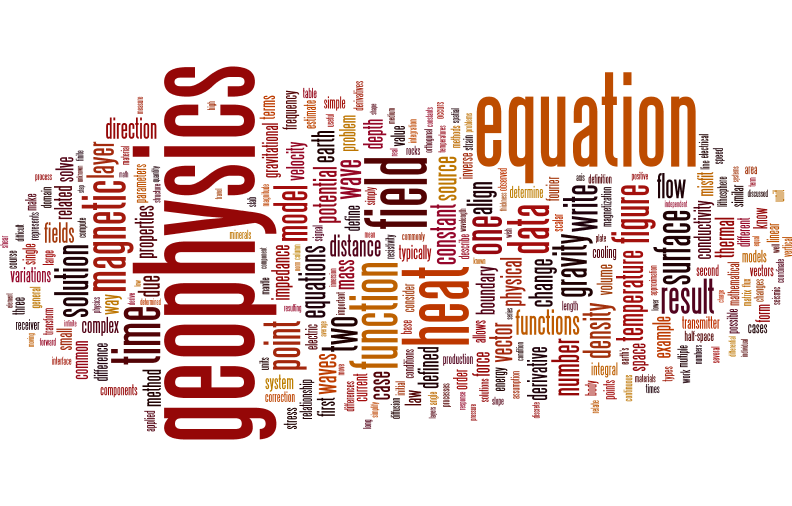
\includegraphics[width=\textwidth,angle=-90]{wordle2.png}
\end{figure}
\clearpage

%\bibliographystyle{elsarticle-harv}
\maketitle
\pagenumbering{roman}
\tableofcontents

\chapter*{Preface}
\phantomsection
\addcontentsline{toc}{chapter}{Preface}

\epigraph{ ``In physical science a first essential step in the direction of learning any subject is to find principles of numerical reckoning and practicable methods for measuring some quality connected with it.  I often say that when you can measure what you are speaking about, and express it in numbers, you know something about it; but when you cannot measure, when you cannot express it in numbers, your knowledge is meagre and unsatisfactory kind; it may be the beginning of knowledge, but you have scarcely, in your thoughts, advanced to the stage of science, whatever the matter may be.''}
{{\normalfont ---\ William Thompson (Lord Kelvin)}}


\section*{Purpose of These Notes}

This text is written for a set of upper-level undergraduate, intermediate to advanced geophysics courses.  It covers a wide range of topics, but is centered around three key equations that are common to many geophysical fields: the potential field, diffusion, and wave equations.  There are several recurring themes drawn from the mathematics of these equations that is returned to over and over again as a device to deepen understanding of the similiarities and differences between geophysical techniques.

Chapters are written to support multiple passes: a first pass focused on concepts and physical meaning, later passes focused on mathematics and implementation.  Text boxes contain mathematical definitions or technical details that can be skipped on a first reading if the concepts are already familiar.  Worked examples illustrate how apply the techniques.

The text is not meant as an exhaustive reference or a numerical analysis text.  The text is supported with recorded lectures that support and extend the concepts in this book.  In class workshops take these concepts and focus on building mathematical intuition and familiarity with properties of Earth Materials and how they vary with lithology. Practical (laboratory) sessions dive further into the mathematics and applications of these techniques computationally.

\section*{How We Use Mathematics in Geophysics}
Like physics, geophysics is a heavily mathematical subject.  Don't panic!  Equations are beautiful.  Yes at times they can cumbersome or complex to derive, but in general the solutions are quite simple and elegant.  Equations on their own do not necessarily tell us much more than the relationship between parameters.  But by knowing the underlying assumptions and understanding the physical meaning of parameters, we can deduce quite a bit about the physical processes operating within the Earth---all by learning to read a humble mathematical statement.

Why derive equations?  While we can measure the relationship between a physical parameter (or several) and an observable, it is often difficult to determine the full extent of the relationship without a proper theoretical basis.  To develop this theoretical basis, we begin with one or more physical principles and apply various assumptions, constraints, boundary conditions, and initial conditions to derive a solution which can be used to model recorded data.  This mathematical journey a derivation.  Once we arrive at our derived solution, we will dissect its meaning by examining its behavior at its extremes in time and/or space.  We can also use the equation to estimate characteristics of the solutions shape, symmetry, and spatial and/or temporal scales.  The derivations that we will pursue in this book arise from simplified cases (often one-dimensional) that illustrate the most basic and essential physical concepts that can often be extended to larger and more complex problems.

Why not start with the solution?  Plugging in numbers is something ``so easy even a caveman can do it.''  One of a geophysicists most valuable skills is their physical intuition.  Unfortunately very few of us are born with innate physical intuition, but it is something that can be gained with practice.  Practice that requires following, studying, dissecting, and performing derivations and their solutions.  While you will not be asked to do many derivations as part of this book, you will be presented with a number of them throughout this book and asked to understand various aspects of their setup, there relation to real world processes, and the implications of their solutions.

\ntextbox{Learning in lectures}{
    It took me a number of years before I properly learned how to learn in lectures (about my 3rd year of undergrad).  The key to learning in a lecture, particularly one with mathematical derivations, is not to write down every word and every step.  Anything that is just rearranging an equation can be easily repeated without writing every step and should not be written down.  Look for the tricks and identify those (e.g.\ a change of coordinates, applying an identity or approximation).  Listen for the key points, be discriminating, think about the concepts as they are presented, and try to forecast the next step.

    We often discuss simplifications of real world processes.  Sometimes they work very well, sometimes less so.  Follow the setup of the problem as it often gives hints for the situations in which it applies.  When do you think it will be applicable?  If you can think of other possible applications bring them up for discussion.

    All of the derivations I will show in class are also in the lecture notes.  Bring them to class and follow along.  Read the notes before hand if you have the time and focus on understanding the parts of the derivation you didn't follow in the notes.  Ask questions.  It is quite likely that there is more than one student with a similar question who also feels intimidated, timid, or too embarrassed to ask.  I don't consider any question to be too basic.
}{aside}

\section*{How to Read and Use the Book}

These notes are structured to flow logically from topic to topic.  Derivations are also structured in a very logical way in order to ease their readability and to emphasize the important concepts. To simplify the reading for you there are some signposts that are meant to identify how much attention you should pay to a particular section of the text.  There are also a lot of equations in the text, though most are intermediate steps in derivations and not important.  Only a handful are required to memorize and a few more that you should pay careful attention to that help build intuition about a particular field.

To signpost specific text, I use numbered boxes whos color indicates the purpose and examples are provided below.
\ntextbox{Core Structure}{These text boxes are the most important to read.  They include key concepts at the start of most chapters, important derivations (though do not need to be memorized) that represent core ideas of geophysical theory.}{core}
\ntextbox{Conventions and Alerts}{These text boxes are meant to make you stop and read.  They are used to designate conventions that may differ from other texts.  They also draw your attention to an important point that may otherwise be overlooked.}{alert}
\ntextbox{Mathematical Tools}{These text boxes include mathematical concepts that are critical to understanding a method or result used in the main text.  You should make sure you understand these concepts.  If you are already familiar with the topic, you may skip them.}{mathtool}
\ntextbox{Perspectives, Aides, and Philosophy}{There are times that I have included additional information or perspectives that are not critical to learning the book content, though they may help.  Sometimes they represent something you might find interesting or wish to explore further outside of class.}{aside}

Not all equations serve the same purpose. Equations marked with a star (\raisebox{-0.4ex}\FiveStar),
\begin{equation}
    \coreeq
    \vb{J} = \grad \phi ,
    \label{eq:memorize}
\end{equation}
are core equations that you should memorize and be able to recall on cue and recognize immediately.  Equations marked with an open star (\raisebox{-0.4ex}\FiveStarOpen),
\begin{equation}
    \workeq
    g_z = \tfrac{4}{3}\pi G a^3 \Delta \rho \frac{z_c}{(x^2 - z_c^2)^{-3/2}} ,
    \label{eq:recognize}
\end{equation}
are important working relations that you should recognize and know how to use.  Most other equations appear only as intermediate steps in derivations and are included to show logical steps and do not require memorization or immediate familiarity and may only make sense in context.  They may appear on their own line,
\[
    \epsilon_{x,x} = \pdv{u_x}{x}
    \label{eq:referenced}
\]
or inline, $h_2 = h_1 + \Delta\varepsilon + r$, and may or may not be numbered.  If numbered it is likely they are an intermediate step in a derivation to be referenced in the text.tract ideas are applied to real problems.

\section*{Mathematical Background and Expectations}

This book assumes prior exposure to calculus, linear algebra, and differential equations at an introductory level. In practice, students arrive with varying degrees of comfort across these topics, and it is common for one or more concepts to require review.

Many mathematical tools are revisited when they are first needed, but they are not re-derived in full generality. For material not reviewed directly in the text, a set of mathematical appendices provides concise summaries of algebra, trigonometry, calculus (derivatives and integrals), complex numbers, vectors and vector calculus, and linear algebra. These appendices are intended as reference material rather than as replacements for prior coursework.

The emphasis throughout the book is not on performing mathematical operations, but on learning to \emph{read} mathematics as a description of physical behavior. A central goal is to develop intuition for how functions behave in space and time, and how changes in parameters affect the geometry and scale of physical responses.

Students are encouraged to build a mental picture of common functional forms.  For example, when an exponential decay is introduced, it should immediately suggest a characteristic length or timescale. When a prefactor multiplies a solution, it should be clear whether it controls overall magnitude, rate of change, or both. Developing this intuition allows you to anticipate how physical properties and spatial or temporal variables influence geophysical anomalies without relying solely on algebraic manipulation.

To support this, a compact reference of common mathematical functions and their graphical behavior is provided, illustrating how constants control scale, curvature, and rate of change. This ability to visualize functions is essential for interpreting geophysical models, assessing plausibility, and understanding the sensitivity of observations to Earth structure.

The goal is therefore not mathematical rigor for its own sake, but an ability to connect mathematical expressions to physical meaning. Mathematics in this book serves as a language for describing the Earth, not an obstacle to understanding it.

\ntextbox{Reading Equations}{
    When you look at the final equation of a derivation in the book, in class, or derived for your assessment, you need to focus on three questions to help understand it's meaning:
    \begin{itemize}
        \item What sets the scale?
        \item What sets the rate of change?
        \item What sets the geometry?
    \end{itemize}
    For example, an exponential decay implies a characteristic length or timescale,
    a Gaussian implies a localized anomaly with a width set by its variance, and a
    sinusoid implies oscillatory behavior with a well-defined wavelength.
}{mathtool}

\section*{Bookkeeping}

\subsection*{Sign Conventions}
Different scientific disciplines adopt different coordinate conventions, often for very practical reasons.  Physicists, astronomers, and engineers typically define the vertical coordinate $z$ as positive upward, away from the Earth. This reflects a worldview in which one studies systems from the outside — looking out or looking up.  Geophysicists, on the other hand, spend most of their time studying what lies beneath their feet. As a result, it is common in geophysics to define the vertical coordinate $z$ as positive downward, into the Earth. In other words, geophysicists look down while physicists look up.  There is nothing fundamentally correct or incorrect about either choice---what matters is consistency. Throughout these notes, unless stated otherwise:
\begin{itemize}
    \item $z$ increases downward
    \item depth is positive
    \item heat flow and gravity are typically treated as positive when directed upward toward the surface
\end{itemize}

When comparing results with other disciplines, textbooks, or software packages, always check the sign conventions carefully. Many apparent “errors” in geophysics reduce to a disagreement about which way is positive.

\subsection*{Units}
The International System of Units (SI) is a triumph of standardization and consistency\ldots and it was designed for laboratory experiments conducted on a workbench.

Geophysics, however, studies a planet.

As a result, geophysicists routinely use scaled or non-SI units that are more natural for the size, duration, and magnitude of Earth processes. Here is a partial list:
\begin{itemize}
    \item distances in kilometres (\si{km}) rather than metres,
    \item times in millions of years\footnote{There is much debate about what units to use to express millions of years in geology.  Different authors opt for various conventions, m.y., \si{Myr}, etc.  We'll use two: $\si{Ma}$ to denote (past) age and age ranges; and \si{My} for model time, future time, or similar time spans.} (\si{My} or \si{Ma}) rather than seconds,
    \item gravity in \si{mGal}\ rather than \si{m.s^{-2}},
    \item magnetic field in \si{nT}\ rather than tesla,
    \item heat flow in \hfu\ rather than \hfu.
\end{itemize}

These choices are not lazy or imprecise — they are pragmatic. Writing Earth-scale numbers exclusively in SI units would obscure physical meaning behind long strings of zeros and make order-of-magnitude reasoning more cumbersome.

Throughout these notes: equations are written to be dimensionally consistent, regardless of unit system, and common geophysical working units are used where they improve clarity.  You are always encouraged to perform a quick check: ``Does this number make physical sense at Earth scale?''

\subsection*{Notation and Conventions}

Throughout this book, notation is chosen to emphasize physical meaning and to remain consistent across different geophysical applications as much as possible. The intent is not to introduce a unique or idiosyncratic notation, but to use a clear and stable set of conventions so that attention can remain focused on the physics rather than on symbols.  While certain symbols (letters, Latin or Greek) are commonly used to denote certain quantities within each subdiscipline, these are rarely standard universally.  Additionally, we use so many symbols throughout the course that there are inevitably some are used more than once to mean very different things.  To reduce confusion, a notation table is given at the start of most chapters that you can quickly use for reference.

Logarithms are quite commonplace in geophysical solutions.  Most of the time, logarithms are base $e$---the natural number. Most programming languages use $\log$ for the natural logarithm so that is the convention we will follow in this book.  When we need a base-10 logarithm, the base will be explicit, $\log_{10}$.  Though I will note that we make plots we typically use $\log_{10}$ instead of $\log$.

We will also frequently need exponentials.  We will sometimes use $\exp$ and $e$ for the natural number, so $\exp(x) = e^{x}$.  The use generally depends on the complexity of the argument, though $\exp$ is used more widely as it is used for $e$ in most computer languages.

Scalars, vectors, and tensors are distinguished explicitly. Scalar quantities (e.g., temperature $T$, pressure $P$, density $\rho$, potential $\phi$) are written as italic symbols. Vector quantities (e.g., displacement $\vb{u}$, gravitational acceleration $\vb{g}$, heat flux $\vb{q}$, magnetic field $\vb{H}$) are denoted using bold symbols, and tensors are written in boldface with appropriate indices (e.g., stress $\bm{sigma}$, strain $\vb{e}$). This distinction is maintained consistently so that the mathematical form of an expression reflects the physical nature of the quantity it represents.

Subscripts and superscripts are used systematically to indicate spatial and temporal indices (e.g., $T_{j,n}$), components (e.g., $g_z$), or reference states (e.g., $T^\circ$). Unless stated otherwise, subscripts typically refer to spatial location or vector component, while superscripts are reserved for time indices or powers. Careful attention to indices is essential for interpreting equations correctly, particularly in numerical formulations where spatial and temporal discretization are made explicit.

Partial ($\pdv{}{z}$) and total derivatives ($\dv{}{z}$) follow standard conventions. Partial derivatives are used when a quantity depends on multiple independent variables, while total derivatives are used when a single independent variable is implied. These distinctions are important for understanding conservation laws and for recognizing the assumptions implicit in governing equations.

\section*{Organization of the Book}

The text is divided into three parts: Fundamentals of Geophysics; Geophysical Fields and Methods; and Computational and Inverse Methods.  Part I introduces physical properies and the general physics of fields.  Part II involves an investigation into the specific properties, classic solutions, and some modern approaches to geophysical fields and how they are used to study the solid Earth.  Part III provides a foundation into mathematical techniques that can be employed to process, model, and invert geophysical fields.  The techniques in Part III have broad utility across (geo)science.  

The mathematical techniques in Part III are woven into the field chapters in Part II.  Because these techniques are so central to the study of modern geophysical fields, they deserve their own consideration that doesn't feel as if the methods can only be used in the one field where an example is demonstrated.  For that reason, I don't expect you to read straight through---rather I anticipate you will want to flip between parts to fully appreciate the subject.  I try to draw specific attention to these connections so that you know when this non-linear approach to reading will be beneficial.

\section*{A Note on Interpretation}

Models are simplified representations of reality, not exact descriptions of the Earth. Every model embodies assumptions about geometry, material properties, boundary conditions, and scales of interest. These assumptions are not flaws; they are choices that make problems tractable and interpretations possible.

Throughout the book, assumptions, approximations, and limitations are discussed explicitly so that analytical and computational results can be interpreted in their proper physical context. Understanding what a model cannot tell us is as important as understanding what it can.

Fourier methods are used extensively in this book as analytical tools for understanding how geophysical fields vary in space and time. By decomposing complex signals into simpler components, Fourier analysis provides insight into scale, symmetry, and attenuation, and allows many problems to be solved or interpreted in closed form. These methods play a central conceptual role, particularly in connecting physical processes to observable patterns.

Finite difference methods are introduced as practical extensions of analytical solutions when geometry, boundary conditions, or material variability become too complex for closed-form treatment. In this course, they are used primarily in computer-based laboratories to explore more realistic geometries and to test physical intuition developed from analytical models. While they are not the primary focus of the topical chapters, they provide an essential bridge between idealized theory and more realistic Earth models.

Inversion theory provides the framework for interpreting geophysical data in terms of subsurface structure and properties. Inverse problems rely on forward models—analytical or numerical—to link physical parameters to observations.  Because these problems are often non-unique and sensitive to noise, inversion requires careful use of constraints, regularization, and physical judgment.  The concepts developed throughout the book culminate in this perspective, where modeling and interpretation come together.

The aim of this book is therefore not to provide definitive answers about the Earth, but to develop the tools and intuition needed to evaluate models critically, compare alternative explanations, and understand how physical assumptions shape geophysical interpretations.

\section*{Acknowledgements}

The geophysics course that this book is designed for started many years before I arrived as a lecturer in geophysics as the University of Adelaide.  It has gone through many revisions as the cohort of students has shifted over the years to varying proportions of physicists, astrophysicists, geologists, and engineers. I first started teaching geophysics with Graham Heinson in 2013 and took over full instruction of the content after a couple of years.  I quickly determined that there was too much content for a single course and so it was separated into two and now, at Adelaide University, it is now three courses (Potential Fields and Geothermics, Electromagnetics, and Seismics).  Ideas in this book come from several foundational works on geophysics Blakely, Telford et al., Grant and West, Lowrie, Fowler, Turcotte and Schubert.  However the idea of using the fundamental PDEs as a throughline came from discussions with fellow graduate students at the University of Utah in David Chapman's research group.  David was an excellent mentor and a phenomenal teacher.  His approach to teaching has heavily influenced the presentation of ideas and information in this text.  My approach is also heavily influenced by my time as an undergraduate at Caltech and the strong connection of geology to physical properties and geophysical fields comes from Don L. Anderson, who always kept at the forefront of his mind the connections between chemistry and physics of the Earth.  While I am nowhere near the calibre of scientist as these two great researchers, I hope that what I have to offer will help inspire you to gain a deeper understanding and appreciation for our wonderful planet and the tools we use to investigate it.


\pagenumbering{arabic}

\part{Fundamentals of Geophysics}
% An introduction to geophysics
\chapter{Geophysics}\label{ch:equations}

This chapter introduces geophysics as a way of thinking about the Earth using physical principles, mathematical models, and quantitative reasoning. Rather than attempting to reproduce geological complexity in detail, geophysics abstracts the Earth into fields, material properties, and governing equations. This abstraction allows us to infer otherwise inaccessible aspects of the Earth—from lithospheric structure and mantle dynamics to groundwater flow, natural hazards, and resource distribution.

The goal of this chapter is to establish a shared conceptual framework that will be used throughout the book. We begin by defining what geophysics is and what it seeks to accomplish. We then introduce the idea of fields and their relationship to material properties, discuss why smooth mathematical descriptions are used to model a discontinuous Earth, and explain why equations and simplified models are essential tools rather than optional conveniences. We conclude with a discussion of how this conceptual framework supports both classical and modern geophysical practice and how it connects to the chapters that follow.

\section{What is Geophysics?}
I'll give two answers the above question, one which you probably suspect.  Firstly, geophysics applies the principles of physics to the study of the Earth and other planetary bodies.  Geophysics is used to probe the structure, composition, physical state, and processes acting with the Earth's interior.  We employ the principles of physics to explore for resources and energy, to monitor the environment and climate, identify and monitor natural hazards, investigate archaeological sites, search for unexploded ordinance, and probe the inner workings of the Earth.

Second, geophysics uses classical physics to model the past, present and future physical state of the Earth---Earth's geological evolution.  Often the Earth can be reduced to a simple process or set of simple processes acting in concert that allow one to identify the key physical processes and properties driving that change.  Through simple models we can see how changes in these key parameters may alter the observed behavior.

It is not possible to cover all of geophysics in one course.  Entire books are written about each of the subdisciplines discussed in these notes.  This course represents a survey of a selected few topics that find applications in industrial and academic settings.  Many of the examples I will use are academic in nature and may, at times, seem far removed from physical reality, but I assure you that the principles and concepts are directly applicable to the real world.

\section{Observation, Abstraction, and Earth Models}

In geophysics, we rarely observe the Earth directly. Instead, we measure physical fields at discrete locations—gravity, magnetic field, temperature, voltage, pressure, or ground motion—and infer the distribution of material properties that produced them. Nearly everything in this book is concerned with relating fields to properties.

Geophysical measurements are indirect, incomplete, and affected by uncertainty. Earth models therefore serve as abstractions that connect observations to physical interpretation. These models are not expected to reproduce the full geological complexity of the Earth but instead to capture the dominant physical processes responsible for the observed data.

\section{Fields}

What is a field?  Each point in space and time may be defined by a set of functions, a {\it field}.  There are three basic types of fields scalars, vectors and tensors.

\emph{Scalar fields} are described by a single function in space and time.  Each point in space has a single magnitude (e.g., density, temperature, pressure).

\emph{Vector fields} are defined by three functions in space and time.  Each point in space has a single magnitude and a direction (e.g., velocity, force, electric field).

\emph{Tensor fields} are technically generalizations of scalar and vector fields, but can be higher order.  Each point in space may be defined by a multiple magnitudes and directions.  While vector fields can be represented by an arrow at each point in space with a length equal to the magnitude and the orientation defining the direction, tensors may be defined by multiple arrows and directions that can be visualized as an ellipse or an ellipsoid at each point in space (e.g., stress, strain, electrical impedance).

Fields can also relate to material properties (e.g., density, magnetization, seismic velocity, resistivity), describe the system states (e.g., temperature, pressure), or force fields that act on each point in space and have the potential to do work (e.g., gravitational attraction, heat flow, strain rate).

Something else that will arise from time to time will be {\it field lines}, which are sometimes refered to as {\it flow lines} depending upon the application. Field lines represent the direction a partical would travel going in the direction of highest magnitude, force, or potential to lowest.  We draw field lines with arrows and they may be open (the ends do not meet) or closed (the ends join).  Although, depending upon the convention, we sometimes draw the arrows in the opposite direction.

In contrast, {\it isolines} trace out a continuous set of points at constant potential, force, or magnitude and are orthogonal ($\perp$) to the field lines at all times.  A common example is contour lines on a topographic map which trace lines of constant elevation.  A rain drop falling on topography would head in the direction of the flow lines.  We can define also define an isosurface or equipotential surface that defines a surface of constant magnitude and can be open like a sheet or closed like a balloon (enclosing a region of space).

\subsection{Continuity and Differentiability}

\emph{The Earth is piecewise discontinuous, but the equations we use assume smoothness.}

Many of the mathematical tools used in geophysics rely on assumptions of continuity and differentiability. These assumptions are often introduced as mathematical requirements, but they also have clear physical interpretations and limitations when applied to the Earth.

The Earth is not a smooth object. Changes in lithology, phase, composition, and structure can produce abrupt changes in material properties such as density, thermal conductivity, elastic moduli, or seismic velocity. As a result, these properties are often discontinuous functions of position.

In contrast, the physical fields we seek to model—such as temperature, gravitational potential, pressure, or displacement—are generally continuous across material boundaries. For example, temperature does not jump abruptly at a lithologic contact, even though the thermal conductivity may. However, the spatial derivatives of these fields need not be continuous. A sharp change in material properties often produces a kink in the field, corresponding to a discontinuity in its gradient.

Most governing equations in geophysics are formulated under the assumption that the relevant fields are continuous and differentiable. These assumptions are required to define derivatives and apply differential operators. When the Earth violates these assumptions, we must either restrict our analysis to regions where the assumptions hold or reformulate the problem in a way that preserves the underlying physical principles, such as conservation of flux.

This distinction between discontinuous properties and continuous fields is central to geophysical modeling. It explains why material interfaces require special treatment, why numerical methods must be designed carefully near sharp contrasts, and why many models enforce smoothness even when the Earth itself is not smooth.

Throughout this book, we will make explicit when continuity and differentiability are assumed, why those assumptions are reasonable, and how their limitations influence both analytic and numerical solutions.  Several of the techniques introduced later in this book can be understood as different ways of managing the tension between a discontinuous Earth and smooth mathematical descriptions.

\section{Geophysical Equations}

There are many partial differential equations (PDEs) but only a handful are commonly used in geophysics.  We will only cover three equations: the potential field equation (Laplace's---or more generally Poisson's equations), the diffusion equation, and the wave equation.  We will study a wide range of physical applications.  Many of these applications are governed by the same or similar equations, differing only by the physical properties that create geophysical fields.

\subsection{Physical Laws and Constitutive Relations}

Governing equations describe the structure of geophysical processes, but they do not by themselves specify how the Earth responds. That information enters through constitutive relations, which link fields such as stress, flux, or current to material properties. These relations determine how forces are transmitted, how energy is transported, and how variations in Earth structure are expressed in observable fields (Chapters~\ref{ch:potential}--\ref{ch:waves}).

Material properties such as density, elastic moduli, electrical conductivity, and thermal diffusivity vary spatially and reflect geological composition, temperature, pressure, and fabric. In this sense, constitutive relations provide the primary connection between abstract equations and the physical Earth. Through these relations, physical properties control how the Earth responds to forcing and how different regions contribute to measured signals. Chapter~\ref{ch:physprop} examines these properties and how they are defined and related to geological materials, providing the link between governing equations and real Earth structure.

Although the governing equations recur across many subdisciplines, differences in material properties and constitutive behavior lead to very different observable phenomena. The essential point here is that geophysical equations acquire physical meaning only when paired with appropriate constitutive relations and property models.

\subsection{Potential Fields} \label{sec:laplace}

No time dependence.

Laplace's and Poisson's equations belong to a special class of partial differential equations called elliptical equations (Chapter~\ref{ch:potential}).  Elliptic equations describe fields that respond instantly to sources (steady-state); parabolic equations describe processes that spread with time (diffiusion); hyperbolic equations describe signals that propagate at finite speed (wave propagation).  These elliptical potential fields equations are defined as
\begin{align}
    \coreeq
    \laplacian u &= 0 & \text{Laplace's equation}, \\
    \coreeq
    \laplacian u &= s & \text{Poisson's equation},
\end{align}
where $u(x,y,z)$ is a scalar potential.  We use Laplace's equation when we are outside of the source region and Poisson's equation within the source region.  A source region is within the body that creates the potential field.  In geophysics, we use these equations to describe gravity, magnetics, voltage, temperature; although the fields must be steady-state (no temporal variation) in order to apply these equations. Poisson's relationship for several geophysical potentials are listed below:
\begin{table}[h!]
    \centering
    \caption{Common uses of the potential fields (elliptical) equation in geophysics.}
    \label{tab:pfeq}
    \begin{tabular}{lcc}
        \toprule
        \textbf{Poisson's Equation} &
        \textbf{Field} &
        \textbf{Chapter} \\
        \midrule
        $\laplacian U = 4 \pi G \rho_m$ & gravity & Ch.~\ref{ch:gravity} \\
        $\laplacian A = -\mu \div \vb{M}$ & magnetics & Ch.~\ref{ch:magnetics} \\
        $\laplacian T = -\frac{A}{k}$ & thermal & Ch.~\ref{ch:geothermics1} \\
        $\laplacian V = -\frac{\rho_e}{\epsilon}$ & electrical & Ch.~\ref{ch:electrostatics}\\
        \bottomrule
    \end{tabular}
\end{table}
While not exactly the same, they are remarkably similar in each case.

\ntextbox{Vector Operators}{
    \begin{center}
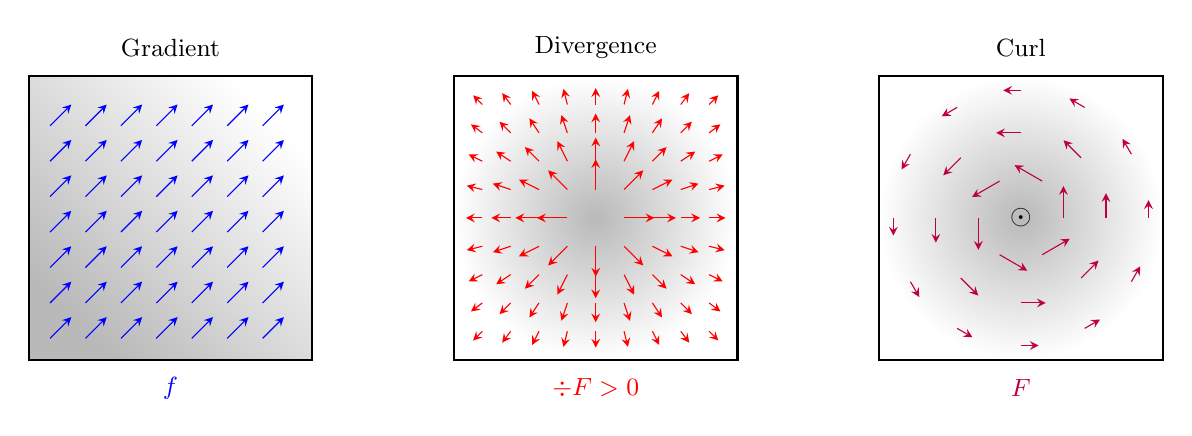
\begin{tikzpicture}[scale=0.9,>=stealth] 
    % Gradient panel 
    \begin{scope} 
        \shade[
            shading=axis,
            left color=gray!55,
            right color=white,
            shading angle=135
        ] (-2,-2) rectangle (2,2);
        \draw[thick] (-2,-2) rectangle (2,2);
        \node at (0,2.4) {\small Gradient};
        \foreach \x in {-1.7,-1.2,...,1.5} 
            \foreach \y in {-1.7,-1.2,...,1.5}
                \draw[->,blue] (\x,\y) -- +(0.3,0.3);
        \node[blue] at (0,-2.4) {\small $\grad{f}$}; 
    \end{scope}

    \begin{scope}[xshift=6cm]
        \shade[
            inner color=gray!55,
            outer color=white,
        ] (-2,-2) rectangle (2,2);
        \draw[thick] (-2,-2) rectangle (2,2);
        \node at (0,2.4) {\small Divergence};

        % Vector field
        \foreach \x in {-1.6,-1.2,...,1.7} {
            \foreach \y in {-1.6,-1.2,...,1.7} {

                % radius
                \pgfmathsetmacro{\r}{sqrt(\x*\x + \y*\y)}

                % avoid division by zero at center
                \ifdim \r pt > 0.05pt

                    % unit vector scaled by decaying function
                    \pgfmathsetmacro{\scale}{0.6/(1 + \r)}

                    \draw[->,red]
                        (\x,\y) --
                        ({\x + \scale*\x/\r}, {\y + \scale*\y/\r});

                \fi
            }
        }

        \node[red] at (0,-2.4) {\small $ \div{\vb{F}} > 0$};
    \end{scope}

    % Curl panel
    \begin{scope}[xshift=12cm]
        \shade[
            inner color=gray!55,
            outer color=white,
        ] (-2,-2) rectangle (2,2);
        \draw[thick] (-2,-2) rectangle (2,2);

        \node at (0,0) {$\odot$};

        \node at (0,2.4) {\small Curl};

        % Inner ring of circulation
        \foreach \a in {0,60,...,330}
            \draw[->,purple] (\a:0.6) -- +(\a+90:0.45);

        \foreach \a in {0,45,...,330}
            \draw[->,purple] (\a:1.2) -- +(\a+90:0.35);

        % Outer ring of circulation
        \foreach \a in {0,30,...,330}
            \draw[->,purple] (\a:1.8) -- +(\a+90:0.25);

        \node[purple] at (0,-2.4) {\small $\curl{\vb{F}}$};
    \end{scope}
\end{tikzpicture}
\textbf{Figure~\thefigure:} Visual depictions of a gradient of a scalar fuction (a), divergence of a vector function (b), and the curl of a vector function (c).
\label{fig:del}
\end{center}


    \textbf{Gradient}, $\grad$, is a linear operator that tells us about the direction of maximum increase (slope) of a field.  Applied to a scalar function, $f$, the gradient is
    \[
        \grad{f} = \pdv{f}{x}\vu{x} + \pdv{f}{y}\vu{y} + \pdv{f}{z}\vu{z}.
    \]
    In geothermics, gradients relate temperature fields to heat flux (e.g., Fourier's law). Physically, the gradient answers the question: \emph{which way is uphill, and how steep is it?}

    We can apply the gradient to a vector field, $\vb{F}$, which results in the Jacobian, a second-order tensor,
    \[
        \grad{\vb{F}} = 
        \begin{bmatrix}
            \pdv{F_x}{x} & \pdv{F_x}{y} & \pdv{F_x}{z} \\[0.4em]
            \pdv{F_y}{x} & \pdv{F_y}{y} & \pdv{F_y}{z} \\[0.4em]
            \pdv{F_z}{x} & \pdv{F_z}{y} & \pdv{F_z}{z} 
        \end{bmatrix} ,
    \]
    and is common in electromagnetics and seismics.

    \medskip \textbf{Divergence}, $\div$, measures the net outward flux of a vector field per unit volume: 
    \[
        \div{\vb{F}} = \pdv{F_x}{x} + \pdv{F_y}{y} + \pdv{F_z}{z} .
    \]
    Positive divergence indicates a source; negative divergence indicates a sink. In the heat equation, divergence expresses conservation of energy by accounting for how heat flows into or out of a volume.

    \medskip \textbf{Curl}, $\curl$, measures the local rotation or circulation of a vector field,
    \[
        \curl{\vb{F}} = 
        \left( \pdv{F_z}{y} - \pdv{F_y}{z} \right) \vu{x} +
        \left( \pdv{F_x}{z} - \pdv{F_z}{x} \right) \vu{y} +
        \left( \pdv{F_y}{x} - \pdv{F_x}{y} \right) \vu{z} .
    \]
    The direction of the curl follows the right-hand rule: pointing your thumb in the direction of the field, your fingers curl in the direction of circulation. Curl is prominent in Maxwell's equations, where it relates time-varying electric and magnetic fields, and it is also central in fluid dynamics through vorticity.

    \medskip \textbf{Laplacian}, $\laplacian = \div \grad$, measures the local curvature of a scalar field,
    \[
        \laplacian f = \pdv[2]{f}{x} + \pdv[2]{f}{y} + \pdv[2]{f}{z} .
    \]
    The Laplacian is features prominantly in the potential, diffusion, and wave equations.
}{mathtool}

\subsection{Diffusion Equation}\label{sec:diffusion}

The diffusion equation belongs to the class of partial differential equations called parabolic equations (Chapter~\ref{ch:diffusion}).  These equations are defined as
\begin{equation}
    \coreeq
    \pdv{u}{t} = D \laplacian u,
\end{equation}
where u(x,y,z) can be either a scalar or vector and $D$ is the diffusion constant.  We can add an additional term to describe motion, making the advection-diffusion equation,
\[
    \pdv{u}{t} = D \laplacian u + \div (V u),
\]
where $V$ is the velocity.

In geoscience, we use the diffusion equation to describe the diffusion of heat and chemical species:
\begin{table}[h!]
    \centering
    \caption{Common uses of the diffusion (parabolic) equation in geophysics.}
    \label{tab:diffusioneq}
    \begin{tabular}{lcc}
        \toprule
        \textbf{Diffusion Equation} &
        \textbf{Field} &
        \textbf{Chapter} \\
        \midrule
        $\pdv{T}{t} = \kappa \laplacian T$ & thermal & Ch.~\ref{ch:geothermics2} \\
        $\pdv{C}{t} = D \laplacian C$ & chemical & --- \\
        $\laplacian \vb{E} = \mu \sigma \pdv{\vb{E}}{t}$ & electrical & Ch.~\ref{ch:EMmethods} \\
        $\laplacian \vb{H} = \mu \sigma \pdv{\vb{H}}{t}$ & magnetic & Ch.~\ref{ch:EMmethods} \\
        \bottomrule
    \end{tabular}
\end{table}
This diffusive form of the electric and magnetic field arises when displacement currents are negligible; we return to these equations in detail in Chapter~\ref{ch:EMmethods}.


\subsection{Wave Equation} \label{sec:waves}
The wave equation belongs to the class of partial differential equations called hyperbolic equations (Chapter~\ref{ch:waves}).  Unlike diffusion, wave solutions transport energy without immediate attenuation and preserve phase information, which is why arrival times are so valuable in seismology.  These equations are defined as
\begin{equation}
    \coreeq
    \pdv[2]{u}{t} = V^2 \laplacian u.
\end{equation}

In geoscience, we use the wave equation to describe propagation of seismic
and electromagnetic waves:

\begin{table}[h!]
    \centering
    \caption{Common uses of the wave (hyperbolic) equation in geophysics.}
    \label{tab:waveeq}
    \begin{tabular}{lcc}
        \toprule
        \textbf{Wave Equation} &
        \textbf{Field} &
        \textbf{Chapter} \\
        \midrule
        $\laplacian \vb{E} = \mu \sigma \pdv{\vb{E}}{t} + \mu \epsilon \pdv[2]{\vb{E}}{t}$ & electrical & Ch.~\ref{ch:EMmethods} \\
        $\laplacian \vb{H} = \mu \sigma \pdv{\vb{H}}{t} + \mu \epsilon \pdv[2]{\vb{H}}{t}$ & magnetic & Ch.~\ref{ch:EMmethods} \\
        $\pdv[2]{\phi}{t} = V_P^2 \laplacian \phi$ & seismic P-wave & Ch.~\ref{ch:seismics} \& \ref{ch:seismology} \\
        $\pdv[2]{\vb{\psi}}{t} = V_S^2 \laplacian \vb{\psi}$ & seismic, S-wave, & Ch.~\ref{ch:seismology} \\ 
        \bottomrule
    \end{tabular}
\end{table}

\section{Solving Geophysical Equations}

A PDE is often the most compact way to describe a physical process mathematically, but the general forms only get us so far.  It is difficult to see how these equations can help locate a buried ore body from a series of gravity measurements, explore how the composition of an Archean lithospheric root affects heat loss at the Earth's surface, or estimate the quality of water resources using electrical currents and magnetic fields we create at the surface.  If we want to solve these problems, we need an understanding of the source and distribution of physical properties and estimates for the boundary and initial conditions.

The problems we generally solve as geophysicts today have very complex geometries (3-D), physical properties that change with the physical state (pressure, temperature, composition), and spatially or temporally varying complex boundary and/or initial conditions.  As it turns out, the methods we use to solve these problems can be relatively simple to think of in mathematical terms, but may give us very limited insight and intution into the behavior of physical fields and how physical properties distort or create them.  Therefore, we will focus our attention largely on analytic solutions to classical problems that can help us make sense of an infinitely more complex Earth.  Unfortunately, these problems can be more difficult to solve, but understanding the approach to these problems can make us better at setting up and solving the physically more complex problems that requir use of a computer.  Developing intuition in geophysics often means thinking in orders of magnitude, which is much easier when the unit system reflects the scale of the Earth rather than the laboratory.

So before we get to the analytic solutions, I want to give you a feeling for how we solve these problems (a more extended discussion of numerical methods are in Chapters~\ref{ch:finitediff} and \ref{ch:inversion}.


\ntextbox{Modeling, Abstraction, and Benchmarks in Geophysics}{
Geophysical models are deliberate abstractions of the Earth, not attempts to reproduce geological reality in full detail. Every model simplifies geometry, material properties, boundary conditions, or physical processes in order to isolate the dominant controls on an observable field. This abstraction is not a weakness of geophysics; it is what makes quantitative interpretation possible. The goal of modeling is not realism, but understanding.  Simple analytic solutions—such as point sources, spheres, cylinders, slabs, or layered half-spaces—play a central role in this process. Although these models are often geologically unrealistic, they serve three indispensable purposes that apply across all geophysical methods.

First, they build physical intuition. Analytic solutions make explicit how geometry, depth, scale, and material contrasts control the amplitude, shape, and spatial extent of observed fields. They reveal which aspects of a problem matter most and which matter least, and they provide scaling relationships that remain valid even when real geology is more complex.

Second, they place quantitative bounds on geological interpretations. Even an oversimplified model can limit what is physically plausible. When the appropriate abstraction is chosen, analytic solutions can constrain minimum depths, maximum density or property contrasts, characteristic length scales, and allowable geometries. A model need not be realistic to be useful; it needs only to capture the controlling physics relevant to the question being asked.

Third, they provide benchmarks for numerical forward and inverse modeling. Analytic solutions define problems for which the correct answer is known. Any numerical code—whether used for forward modeling, inversion, discretized Earth representations, or AI-assisted workflows—should be able to reproduce these solutions to within expected numerical tolerance. If a code cannot recover the response of a simple analytic model under appropriate conditions, then the problem lies with the implementation, not with the geology. Analytic benchmarks therefore act as calibration standards for computational geophysics and geodynamics.

These principles apply to potential fields, diffusion, wave propagation, and inverse problems alike. As the course progresses, analytic models will repeatedly appear—not as literal representations of the Earth, but as tools for reasoning, bounding interpretations, and validating more complex numerical approaches.  For this reason, many of the analytic solutions introduced in this course serve a dual role: they clarify the behavior of governing equations and provide reference cases against which numerical solutions can be tested.
}{aside}

\section{Correcting and Transforming Geophysical Data}

Geophysical data are rarely interpreted in the form in which they are first measured. Observations reflect not only the target of interest but also acquisition geometry, reference frames, interfering sources, and processes operating at scales outside the problem being addressed. As a result, geophysical analysis commonly begins with corrections and transformations that place data into a physically meaningful form before modeling or interpretation.

Many of these operations are most naturally expressed as linear transformations of fields. Fourier-based methods are particularly useful because they exploit linearity and superposition, allowing differential operators to be represented as algebraic ones and scale-dependent behavior to be examined explicitly. In potential-field geophysics, Fourier transforms underpin upward and downward continuation, regional-residual separation, and transformations such as reduction to the pole, reduction to the equator, and pseudogravity. Isostatic corrections to gravity data similarly involve modeling and removing long-wavelength contributions associated with lithospheric compensation. In magnetics, these operations provide a way to relate observed anomalies to equivalent sources under different assumptions about magnetization and geometry.

Transform methods are equally central in other areas of geophysics. In wave-based problems, Fourier and related transforms are used to analyze dispersion, attenuation, and bandwidth, and to separate signals in time, frequency, or wavenumber domains in seismology and electromagnetics. In diffusive systems, transforms provide insight into penetration depth, characteristic time scales, and filtering behavior. Corrections applied in geothermics and paleoclimate studies—such as adjustments for topography, elevation, or long-term background trends—also rely on separating signals by scale, even when the underlying implementation is not explicitly framed in the frequency domain. Chapter~\ref{ch:fourier} develops Fourier methods systematically, but throughout this book these techniques should be viewed less as specialized tools than as a general language for understanding scale, resolution, and transformation in geophysical data.

\subsection{Simplified view of PDE's}

The geophysical equations we discuss above may look complicated because of the vector calculus representation, so lets demystify that a bit.  Above, we used the del---also called nabla, from Greek for harp---(upside-down triangle, $\nabla$) to denote a spatial derivative in multiple dimensions.  You may notice that in most equations above, we are using del-squared known as the Laplacian, $\laplacian$, operator.  We'll talk more about what this means later, but for now
\[
    \laplacian = \pdv[2]{}{x} + \pdv[2]{}{y} + \pdv[2]{}{z} .
\]
If we only had one spatial dimension (say $x$), or all fields are constant in the other two (i.e. unchanging in $y$, and $z$), then the above expression reduces to
\[
    \laplacian = \pdv[2]{}{x} .
\]
which simply denotes the second derivative with respect to the spatial variable $x$.  I will explain what this means in simpler terms below.

Let us suppose we have an elevation profile along a hike, $E$, where $E(x)$ represents the elevation along our profile at the position $x$.  If we wanted to find the second derivative of our elevation field, $E$, we would write it as
\[
    \pdv[2]{E}{x} .
\]
We'll start with a first derivative ($\pdv{E}{x}$) and then look at what
happens when we take the second (Figure~\ref{fig:dtopo}).
\begin{figure}[htb]
    \centering
    \includegraphics[width=\textwidth]{introduction/figures/andes_topo.eps}
    \caption{Elevation and derivatives for the Andes at 9$^\circ$S.  (a)
    Observed elevtion at 2' resolution.  (b) First-derivative of elevation
    produces the topographic slope.  (c) Second-derivative of elevation results
    in the topographic curvature (the rate in change of slope).}
    \label{fig:dtopo}
\end{figure}

A derivative is a concept that represents the slope of a line that is tangent to a curve or plane; that is the line touches the curve but does not cross it.  In our example, the first derivative represents the topographic slope.  For those of you that have done some field mapping, you could also conceptualize the derivative as the dip angle of a compass you place on a bedding plane.  If we were standing at position $x_1$, we could approximate the topographic slope as the change in elevation over a small distance about our location, i.e.,
\[
    e(x_1) \approx \frac{E(x_2) - E(x_1)}{x_2 - x_1} .
\]
Although this description is not the derivative, it gives us the means by which we can approximate it.  By choosing the position $x_1$ that we wish to know a tangent's slope and a second point very near the first, we arrive at a estimate of the derivative.  This \textbf{finite-difference} view is the basis for many numerical solutions to PDEs, including the finite-difference methods introduced later in Chapter~\ref{ch:finitediff}.  The definition of a derivative is similar to the above such that the position of the second point is meant to approach the first until the two become so close that their distance is effectively zero.

So what is a derivative?  A derivative is the change in a field/function relative to another.  A second derivative, is simply the rate at which the slope changes.  We call this rate in change of slope the curvature.  We can find the curvature by applying the same logic as above to our slope, $e$.  That is, the curvature is approximated by
\[
    \xi(x_1) \approx \frac{e(x_2) - e(x_1)}{x_2 - x_1} .
    \label{eq:curvature}
\]
You may notice that the curvature requires that we know the slope at two points, $x_1$ and $x_2$, which we approximated above for only $x_1$.  Therefore, we need to approximate $e(x_2)$ as well, which will require a third point, i.e., $e(x_2) = (E(x_3) - E(x_2))/(x_3 - x_2)$.  Let us be smart and choose our positions $x_1$, $x_2$, and $x_3$ such that the differences are constant: $x_2$ - $x_1$ = $x_3$ - $x_2$.  In this case, we can replace both differences in distance with a constant, which we will denote by $\Delta\! x$ to simplify our expressions.  Substituting our simplified expressions for $e(x_1)$ and $e(x_2)$ into Equation~\ref{eq:curvature}, we find the curvature can be approximated by
\[
    \xi(x_1) \approx \frac{ E_3 - E_1 }{\Delta\! x^2} .
\]
Although there are more accurate ways to estimate a derivative, this approach is common because it is straightforward and allows us to compute a derivative very easily.  A computer may not know what a derivative is, but it can be easily programmed to subtract, divide and raise to a power.

Figure~\ref{fig:dtopo} illustrates the results of a derivative of topography with respect to position along a transect at 9$^\circ$S across the Andean subduction zone and Andes Mountains.  Notice that when topography changes rapidly the derivative is large and when the change is topography is small the derivative is also small (Figure~\ref{fig:dtopo}).  Beyond telling us how rapidly a function changes, a derivative can also amplify those changes.  One of the most powerful aspects of a derivative is the ability to identify a functions maxima and minima.  We'll explore some of these and additional uses further throughout the course.

\subsection{Principle of Superposition}\label{sec:superposition}

Many geophysical processes are well approximated as linear systems. Linearity requires two conditions:
(1) \emph{additivity};
\begin{equation}
    \coreeq
    f(m_1 + m_2 + \cdots) = f(m_1) + f(m_2) + \cdots,
\end{equation}
and (2) \emph{homogeneity},
\begin{equation}
    \coreeq
    f(a\omega) = a f(\omega).
\end{equation}
When these conditions hold, the \emph{principle of superposition}\footnote{The mathematical principle of superposition differs from the geological concept of superposition, which is about how sedimentary layers are deposited on top of earlier layers.} applies. This principle is fundamental to gravity, magnetics, electrostatics, many wave phenomena, and diffusive processes at sufficiently small amplitudes.

The {\it principle of superposition} allows us to construct the total response function by summing the independent responses functions due all individual sources.  At times, we will use superposition to deconstruct solutions, removing background effects and isolating anomalies.  We will also use superposition to build solutions to elliptical and parabolic PDE's using Fourier series (Chapter~\ref{ch:fourier_series}).

Some Earth processes inhibit our ability to use superposition, creating non-linearity in field responses.  Non-linear processes, such as plastic deformation, melting, or strongly temperature-dependent transport, violate superposition and require more complex solution strategies.

Linearity conditions will be revisited again for a different context in Chapter~\ref{ch:inversion}. 


\ntextbox{Example (Linearity and Superposition)}{
    If a mass $m_1$ produces a gravitational acceleration $\mathbf{g}_1$ at an observation point, and a second mass $m_2$ produces $\mathbf{g}_2$, then placing both masses together produces
    \[
    \mathbf{g} = \mathbf{g}_1 + \mathbf{g}_2 .
    \]
    Doubling either mass doubles its contribution to the total field. This linear behavior allows complex mass distributions to be built up by summing the effects of simpler components.
}{mathtool}

Superposition applies to computing the fields associated with electrical charges, magnetic moments, and gravitational masses (at least in the classical limit).  It also holds for many wave and diffusive processes.  Although this typically requires that the amplitude is small compared to the wavelength.

Most of the PDE's we will solve are considered linear differential equations and as a result allow us to superimpose solutions. Non-linear processes such as plastic deformation, melting, or strongly temperature-dependent conductivity violate superposition and require different solution approaches.

\subsection{Forward and Inverse Problems}

Solving a geophysical equation always involves answering a specific physical question. In its most basic form, this question can be stated as follows: given a description of the Earth and the physical laws governing a process, what observations should we expect to measure? This question defines the \emph{forward problem} and is the starting point for nearly all quantitative geophysical analysis.

In a forward problem, the Earth is represented by a model consisting of geometry, material properties, sources, and boundary or initial conditions. The governing equations introduced in the previous section are then solved to predict observable fields such as gravity anomalies, surface displacements, temperatures, or waveforms. Forward problems are typically well defined: for a given model and a specified set of equations, a unique prediction can be computed, at least in principle. Much of this book is devoted to building physical intuition about forward models and understanding how different components of an Earth model influence the resulting fields.

Inference enters because geophysical observations are indirect. In practice, we observe fields at a finite number of locations, often with noise and incomplete spatial or temporal coverage. Interpreting these observations requires reasoning backward from effects to causes. Rather than solving equations once, we solve them repeatedly while varying model parameters in order to explore how changes in structure or properties affect predicted data. This process links physical understanding to interpretation long before any formal inverse method is applied.

The \emph{inverse problem} formalizes this backward reasoning. Instead of predicting data from a known model, the inverse problem asks which Earth models are consistent with a set of observations. This question is fundamentally different from the forward problem. Multiple models may explain the same data, small data errors may produce large changes in inferred parameters, and additional assumptions are required to select among competing solutions. These issues are not pathologies of particular datasets or methods; they are intrinsic to the indirect nature of geophysical observation.

At this stage, it is important to emphasize that inversion does not replace forward modeling. Forward problems define the physics, determine sensitivity to model parameters, and establish the limits of what data can constrain. Inversion provides a structured framework for exploring model space, managing uncertainty, and making assumptions explicit. For this reason, forward modeling remains central even in highly automated or data-intensive workflows.

Formal inversion theory, including questions of non-uniqueness, instability, and regularization, is developed in Chapter~\ref{ch:inversion}. Here, the essential point is that forward modeling, inference, and inversion are not separate activities but parts of a continuous reasoning process. Solving geophysical equations is therefore not an end in itself but a means of connecting physical laws, Earth properties, and observational data in a logically consistent way.

\section{The Changing Practice of Geophysics}

Over the past several decades, the practice of geophysics has undergone repeated transformations: from analytic solutions worked out by hand, to numerical modelling on desktops and supercomputers, to large-scale inversion and simulation on modern computers, and from one- and two-dimensional analyses to fully three-dimensional volumes of data. We are now entering another transition period, driven by the rapid development of artificial intelligence (AI) tools for learning, literature review, coding, and data analysis.

AI systems can help explore unfamiliar literature, suggest alternative formulations of a problem, generate code quickly, and draw connections that we might not immediately recognize. Used wisely, these tools can accelerate idea testing, reduce time spent on repetitive tasks, and allow us to explore a broader range of hypotheses than would otherwise be practical.

However, AI does not remove the need to understand geophysics---it increases it.

AI systems do not know physics. They reproduce patterns present in their training data, which means they can:
\begin{itemize}
    \item silently violate assumptions such as linearity, causality, or conservation laws,
    \item apply an inappropriate sign convention or unit system,
    \item produce code that runs but solves the wrong equation, or
    \item generate visually convincing results that are physically incorrect.
\end{itemize}

The only reliable safeguard against these errors is physical intuition: an understanding of governing equations, scaling behavior, characteristic length and time scales, and the meaning of parameters. Additionally, the classic analytic solutions are reliable tests of codes, whether written by AI or humans.  Without a geophysical foundation, it becomes easy to accept outputs that look reasonable but produce incorrect models and lead to flawed conclusions.

For this reason, the goal of this course sequence is not to train you to compete with automated tools, but to train you to use them effectively and critically. Understanding the basics — fields, governing equations, superposition, diffusion, wave propagation, and inversion — allows you to:
\begin{enumerate}
    \item design experiments and surveys for maximum information content,
    \item recognize when a model result is implausible,
    \item identify when assumptions have been violated, and
    \item justify conclusions defensibly, rather than merely reporting them.
\end{enumerate}

Geophysics has always advanced by combining new tools and techniques with careful physical reasoning. AI is simply the latest tool in that lineage. Mastery of the fundamentals ensures it remains an ally rather than a liability.

Intended capstone discussion of analytic vs numerical vs computational methods, data volume, uncertainty, and modern workflows.

Throughout this chapter, we have emphasized a common conceptual structure that underlies all of geophysics. Observable fields provide our primary window into the Earth, governing equations describe how those fields behave, and the solutions to those equations reveal how geometry, boundary conditions, and scale control what can be measured. Interpretation then requires inference: reasoning from observed fields back to the Earth models that could have produced them. Material properties play a dual role in this framework. They generate and modify fields through constitutive relations, yet their spatial distribution is rarely known a priori and must be constrained through forward modeling and, ultimately, inversion. The chapters that follow elaborate this structure in different physical contexts, but the underlying logic remains the same.


% Physical properties
\chapter{Properties of Earth Materials}\label{ch:physprop}

\section{Introduction}
To ground our theoretical exploration of many fields, it is important to remember that we are trying to learn about the physical state and composition of a real system.  The geophysical fields explored in this course do not arise directly from geology, but from the physical properties of Earth materials.  Physical properties are intrinsic material parameters---or combinations of them---that control how rocks generate, modify, or respond to geophysical fields.  In this chapter, we introduce the key material properties that govern geophysical fields and how they vary with state conditions. Later chapters return to these properties repeatedly in different physical contexts.

\begin{enumerate}
    \item Gravity \& magnetics: Density appears explicity in formulation of the gravitational potential.
    \item Magnetics: Susceptibility is obscured somewhat by the use magnetization.
    \item Geothermics: Thermal conductivity, density, specific heat capacity and heat production are integral to the heat equation.
    \item Electromagnetics: Electrical conductivity/resistivity dominates EM responses and depends strongly on fluids, temperature, and connectivity.
    \item Seismology: Seismic velocities are emergent properties controlled by elastic moduli, density, and microstructure.
\end{enumerate}

To make sense of how different properties enter geophysical equations and how they are estimated in practice, it is useful to distinguish between several broad classes of material properties.

\subsection{Types of properties}

Material properties encountered in geophysics fall into several broad categories: intrinsic, derived, and compositional (e.g., Table~\ref{tab:prop_summary}). Intrinsic properties, such as density, elastic moduli, heat capacity, and thermal expansivity, arise from thermodynamic and mechanical response functions and describe how materials respond to changes in pressure, temperature, or stress. Derived (or emergent) properties, such as seismic velocity or thermal diffusivity, are derived quantities formed by combining intrinsic parameters through governing equations.  Intrinsic properties describe material response; derived properties combine intrinsic parameters and often amplify ambiguity in interpretation.
\begin{table}
    \centering
    \begin{threeparttable}
    \caption{Selected physical properties relevant to geophysical fields.}
    \label{tab:prop_summary}
    \begin{tabular}{@{}llccl@{}}
        \toprule
        \textbf{Symbol} &
        \textbf{Property} &
        \textbf{Type}\tnote{a} &
        \textbf{Primary fields} &
        \textbf{Introduced in} \\
        \midrule
        $\rho$   & density & intrinsic & gravity, seismic & \S\ref{sec:density} \\
        $\chi$   & magnetic susceptibility & compositional & magnetics & Ch.~\ref{ch:magnetics} \\
        $K$      & bulk modulus & intrinsic & seismic & \S\ref{sec:bulk_modulus} \\
        $\mu$    & shear modulus & intrinsic & seismic & \S\ref{sec:shear_modulus} \\
        $V_P$    & P-wave velocity & derived & seismic & \S\ref{sec:velocity} \\
        $V_S$    & S-wave velocity & derived & seismic & \S\ref{sec:velocity} \\
        $k$      & thermal conductivity & intrinsic & thermal & \S\ref{sec:thermal_cond} \\
        $\kappa$ & thermal diffusivity & derived & thermal, EM & \S\ref{sec:diffusivity} \\
        $A$      & heat production & compositional & thermal & Ch.~\ref{ch:geothermics1} \\
        $C_P$    & heat capacity & intrinsic & thermal & \S\ref{sec:heat_cap} \\
        $\sigma$ & electrical conductivity & intrinsic & EM & Ch.~\ref{ch:EMmethods} \\
        \bottomrule
    \end{tabular}
    \begin{tablenotes}
        \item[a] Intrinsic properties describe material response; derived properties combine intrinsic parameters and often amplify ambiguity in interpretation.
    \end{tablenotes}
\end{threeparttable}
\end{table}

While all properties are compositionally dependent to some degree, a third class of properties depends primarily on composition and mineralogy rather than thermodynamic derivatives. These include source terms such as radiogenic heat production, which depends on the abundance of radioactive isotopes, and coupling parameters such as magnetic susceptibility, which controls how strongly a material responds to an applied magnetic field. These properties are often weakly state dependent but can vary by orders of magnitude with composition.

Most physical properties of rocks are not constant, but change as state conditions change (pressure and temperature).  Composition is an important control, as are the crystallographic structure, crystal orientation, crystal defects, porosity, and grain size.  There are several methods that one may use to estimate physical properties including by oxide composition, mineralogy, and thermodynamic modeling.  Each have their own drawbacks and advantages. As a result, the way physical properties are estimated is often as important as the properties themselves.

\section{State variables and material response}
Many physical properties of Earth materials vary as a function of state conditions: primarily pressure, temperature, volume, and composition (e.g., Figure~\ref{fig:velocity_state}).  A familiar example that makes this dependence explicit is the ideal gas law,
\[
    PV = nRT
\]
where $P$ is pressure, $V$ is volume, $T$ is temperature, $n$ is the amount of material (we will typically use $X$ for composition), and $R$ is the gas constant.
\begin{figure}[tbh]
    \centering
    \includegraphics[]{physprop/figures/vp_granite_gabbro.eps} 
    \caption{Laboratory measurements of compressional wave velocity as a function of pressure and temperature for granite and gabbro \citep{Christensen&Mooney1995}. At low pressures, open microcracks strongly reduce seismic velocity, particularly in felsic rocks. Increasing pressure closes cracks and increases velocity, while increasing temperature reduces velocity through thermal expansion and elastic softening. Compositional differences between granite and gabbro persist even at high pressure, illustrating the combined influence of pressure, temperature, composition, and near-surface crack porosity on seismic velocity.}
    \label{fig:velocity_state}
\end{figure}

Although the ideal gas law applies strictly to gases and is not valid for solids, it provides a useful conceptual framework: it makes clear that material properties such as density cannot be treated as fixed constants, but emerge from the interaction between intrinsic material characteristics and state variables.

For solids and liquids in the Earth, different constitutive relations are required, involving elastic moduli, thermal expansion, compressibility, and phase equilibria. Nevertheless, the same fundamental idea applies: changes in pressure, temperature, or composition lead to changes in physical properties, which in turn modify the geophysical fields we observe.

In the sections that follow, we describe the relevant constitutive relationships appropriate for Earth materials and examine how physical properties respond to state conditions within the Earth.

Many geophysical inverse problems can be viewed as attempts to infer spatial variations in state-dependent material properties from measurements of physical fields.


\subsection{Estimating physical properties}
In practice, physical properties of Earth materials are rarely known exactly and must be estimated using a range of complementary approaches. These approaches differ in their required inputs, assumptions, flexibility, and accuracy, and no single method is universally superior.

Oxide-based models often employ simple empirical relationships between bulk chemical composition and physical properties. These models are easy to apply and computationally efficient, but they are generally the least flexible and may extrapolate poorly beyond their calibrated compositional range.

Mineralogical models estimate properties from modal mineralogy and laboratory-measured mineral constants. These approaches can incorporate crystal orientation and compositional layering and may be calibrated over a range of pressure and temperature conditions. However, they require reliable estimates of mineral proportions and do not guarantee that the inferred mineral assemblage is thermodynamically stable.

Thermodynamic models provide a self-consistent framework for estimating stable mineral assemblages and associated physical properties as a function of pressure, temperature, and composition. These methods are powerful but computationally intensive and generally cannot incorporate geometric effects such as porosity, cracks, or fabric without additional assumptions.

The appropriate estimation strategy depends on the desired accuracy, available information, spatial scale, and physical context. Accordingly, the formulas and tables presented in this chapter should be viewed not as exact prescriptions, but as tools that must be applied with an understanding of their assumptions and limitations.

The methods described here pertain primarily to igneous and metamorphic rocks in the absence of a fluid phase. Near the surface, porosity and cracks often exert additional controls on physical properties that are not easily captured in these frameworks and must be treated separately (Section~\ref{sec:porosity}).

The goal of this chapter is not to prescribe a single workflow for estimating properties, but to provide the physical relationships and reference values needed to make informed choices in different geophysical contexts.  Each of the properties listed above is introduced in detail below, with emphasis on physical meaning, state dependence, and relevance to geophysical observations.


% Density
\section{$P$ \& $T$ effects on properties} \label{sec:prop_eq}
The estimation of physical properties for various minerals in this section are derived from numerous laboratory experiments.  The mathematical forms are given below require lab-derived empirical constants specific to each mineral resulting from idealized end-member compositions (Table~\ref{tab:physprop}).
\newcommand{\splitcell}[2][c]{%
  \begin{tabular}[#1]{@{}c@{}}#2\end{tabular}}

\begin{landscape}
\begin{table}
    \centering
    \begin{threeparttable}
    \caption{Empirically derived constants used to compute physical properties
    of rocks. These values are intended as representative laboratory measurements and should not be interpreted as fixed constants within the Earth.}
    \label{tab:physprop}
    \tiny
    \begin{tabular}{@{}llcccccccccccccccccc@{}}
        \toprule
        \textbf{mineral} & \textbf{formula unit} &
            \splitcell{\textbf{formula}\\\textbf{weight}\\(\si{g.mol^{-1}})} &
            \splitcell{\textbf{molar}\\\textbf{volume}\tnote{a}\\(\si{cm^3.mol^{-1}})} &
            \splitcell{\textbf{density}\\@\SI{298}{K}\\(\si{kg.m^{-3}})} &
            \splitcell{\ce{H2O}\\\si{wt\%}}  &
            \multicolumn{3}{c}{\splitcell{\textbf{expansivity}\\$\alpha = a_0 + a_1 T + a_2 T^{-2}$\\(K$^{-1}$)}} &
            \multicolumn{4}{c}{\splitcell{\textbf{specific heat capacity}\\$C_{P} = c_0 + c_1 T^{-0.5} + c_2 T^{-2} + c_3 T^{-3}$\\(\si{kJ.kg^{-1}.K^{-1}})}} &
            \splitcell{\textbf{isothermal} \\ \textbf{bulk} \\ \textbf{modulus}\\(\si{GPa})} & $\dv{K_T}{P}$ &
            \splitcell{\textbf{shear} \\ \textbf{modulus} \\ (\si{GPa})} & $\dv{\ln \mu}{\ln \rho}$ & $\dv{\mu}{P}$ &
            \splitcell{\textbf{Gr{\"u}neisen} \\ \textbf{parameter}} &
            \splitcell{\textbf{Anderson-} \\ \textbf{Gr{\"u}neisen} \\ \textbf{parameter}} \\
        {} & {} &
            $m_{fu}$ &
            $V^\circ$ &
            $\rho^\circ$ &
            {} &
            $a_0 \times 10^5$ & $a_1 \times 10^8$ & $a_2$ &
            $c_0$ & $c_1$ & $c_2$ & $c_3$ &
            $K_T^\circ$ & $K_T'$ &
            $\mu^\circ$ & $\Gamma$ & $\mu'$ & $\gamma_{th}$ & $\delta_T$ \\
        \midrule
        $\alpha$-quartz & \ce{SiO2} &
            60.1 &
            22.7 &
            2648 &
            0 &
            1.417 & 9.6581 & -1.6973 &
            1.7699 & -23.49 & 45.947 & -7.2006 &
            37.12 & 5.99 &
            44.80 & 40.1 & 0.46 &
            0.7 & 8.42 \\
        $\beta$-quartz & \ce{SiO2} &
            60.1 & 22.7 & 2530 & 0 & -0.44 & 0 & 0 & 0.9647 & -0.0004
            & 30.546 & -0.0018 & 57.01 & 4.00 & 41.40 & 4.1 & 1.21 & 0.1 & 4.11 \\
            orthoclase & KAlSi3O8 & 278.3 & 105.1 & 2555 & 0 & 3.4 & 0 & 0 & 1.4445 &
            -9.5303 & -26.395 & 3.6781 & 58.30 & 4.00 & 28.10 & 4.4 & 0.80 & 0.4 & 4.44 \\
        albite & \ce{NaAlSi3O8} &
            262.2 &
            99.0 &
            2620 &
            0 &
            1.9801 & 1.0065 & -0.976 &
            1.5012 & -9.2116 & -30.099 & 4.0829 &
            57.76 & 4.00 &
            29.78 & 13.0 & 1.21 &
            0.6 & 4.57 \\
        anorthite & \ce{CaAlSi2O8} &
            278.2 &
            105.0 &
            2760 &
            0 &
            1.2491 & -0.0162 & 0.0161 &
            1.5793 & -4.7252 & 0 & -1.1395 &
            81.86 & 4.00 &
            36.05 & 6.8 & 3.48 &
            0.5 & 4.47 \\
        muscovite & \ce{KAl3Si3O10(OH)2} &
            398.2 &
            150.4 &
            2828 &
            4.5 &
            3.537 & 0 & 0 &
            1.668 & -10.994 & -36.79 & 5.0614 &
            49.00 & 4.00 &
            29.54 & 4.5 & 1.00 &
            0.5 & 4.52 \\
        phlogopite & \ce{KMg3AlSi3O10(F,OH)2} &
            417.2 &
            157.6 &
            2788 &
            4.5 &
            5.8 & 0 & 0 &
            1.4354 & -4.0508 & -61.28 & 8.995 &
            49.70 & 8.59 &
            22.94 & 9.1 & 0.77
            & 0.6 & 9.14 \\
        annite & \ce{KFe3AlSi3O10(F,OH)2} &
            511.9 &
            193.3 &
            3317 &
            3.5 &
            3.7 & 0 & 0 &
            1.2777 & -5.661 & -42.813 & 6.9201 &
            49.70 & 8.59 &
            22.94 & 9.1 & 0.77 &
            0.6 & 9.14 \\
        hornblende & \ce{Ca2(Mg,Fe,Al)5(Al,Si)8O22(OH)2} &
            864.7 &
            326.6 &
            3248 &
            2.5 &
            2.075 & 1.027 & 0 & 
            1.6559 & -13.126 & 1.5163 & -2.6059 &
            93.97 & 4.00 &
            54.50 & 5.1 & 0.97 &
            1.1 & 5.10 \\
        diopside & \ce{CaMgSi2O6} &
            216.6 &
            81.8 &
            3272 &
            0 &
            3.33 & 0 & 0 &
            1.4103 & -7.4109 & -33.09 & 4.2567 &
            113.00 & 4.80 &
            64.90 & 6.0 & 2.00 &
            1.2 & 6.04 \\
        hedenbergite & \ce{CaFeSi2O6} &
            248.1 &
            93.7 &
            3651 &
            0 &
            2.98 & 0 & 0 &
            1.3712 & -10.668 & -32.729 & -0.0042 &
            119.20 & 4.00 &
            61.00 & 5.2 & 0.85 &
            1.2 & 5.21 \\
        enstatite & \ce{MgSiO3} &
            200.8 &
            75.8 & 
            3206 &
            0 &
            2.972 & 0.5711 & 0 & 
            1.6592 & -11.959 & -22.616 & 2.7805 &
            105.80 & 8.50 &
            76.80 & 9.4 & 2.00 &
            0.9 & 9.39 \\
        ferrosilite & \ce{FeSiO3} &
            263.9 &
            99.6 &
            4003 &
            0 &
            2.875 & 0 & 0 &
            1.3204 & -10.559 & -3.444 & -0.2858 &
            100.17 & 4.00 &
            52.00 & 5.1 & 2.00 &
            1.1 & 5.05 \\
        forsterite & \ce{Mg2SiO4} &
            140.7 &
            53.1 &
            3222 &
            0 &
            2.854 & 1.008 & -0.3842 &
            1.6572 & -12.804 & 0 & -1.9042 &
            127.30 & 5.37 &
            81.60 & 5.2 & 1.82 &
            1.2 & 5.50 \\
        fayalite & \ce{Fe2SiO4} &
            203.8 &
            77.0 &
            4400 &
            0 &
            2.386 & 1.153 & -0.0518 &
            1.2366 & -9.882 & 0 & -0.3052 &
            136.70 & 5.16 &
            51.00 & 4.7 & 0.62 &
            1.1 & 5.40 \\
        spinel & \ce{MgAl2O4} &
            142.3 &
            53.7 &
            3575 &
            0 & 
            1.96 & 1.64 & 0 &
            1.7197 & -14.086 & 0 & 0 & 
            196.20 & 4.00 &
            107.81 & 4.2 & 0.92 &
            1.3 & 6.50 \\
        pyrope & \ce{Mg3Al2Si3O12} &
            403.1 &
            152.2 & 
            3565 &
            0 &
            2.311 & 0.5956 & -0.4538 &
            1.4657 & -7.012 & -33.042 & 3.1262 &
            173.81 & 5.00 &
            94.00 & 4.1 & 1.50 &
            1.3 & 5.30 \\
        almandine & \ce{Fe3Al2Si3O{12}} &
            497.7 &
            188.0 &
            4324 &
            0 &
            1.776 & 1.214 & -0.5071 &
            1.2485 & -6.605 & -30.298 & 4.4437 &
            174.10 & 6.00 &
            92.10 & 5.5 & 1.60 &
            1.0 & 5.52 \\
        \bottomrule
    \end{tabular}
    \begin{tablenotes}
        \item Expansivity constants and specific heat capacity from {\citet{Hasterok&Chapman2011}} and references therein.  All other values from \citet{Hacker_etal2003} and references therein.
        \item[a] The $^\circ$ indicates conditions at 0.1~MPa and 298~K.
    \end{tablenotes}
\end{threeparttable}
\end{table}
\end{landscape}


\ntextbox{Standard Temperature and Pressure (STP)}{
    Standard temperature and pressure (STP) is a state convention for laboratory measurements.  These may vary from study to study depending on which convention they are using.  The most commonly used standard pressure is $\SI{1}{atm} \approx \SI{0.1}{MPa}$.  Standard temperature tends be less consistent but is typically \SI{298}{K}\ (25~\degC), though is often \SI{273}{K} (\SI{0}{\degC})

}{alert}\label{box:stp}

\subsection{Density, $\rho$ [kg~m$^{-3}$]} \label{sec:density}
Density is the ratio of a unit mass to a specified volume.  The density at
298~K is determined by the formula weight per molar volume, i.e.,
$\rho^\circ = m_\mathrm{fu} (V^\circ)^{-1}$.  However, very little of the Earth
is at 298~K (25\degC) and atmospheric pressure (0.1~MPa). Rock density
changes in response to the higher temperatures and pressures found internal
to the Earth.  Therefore, in order to appropriately model density, we must,
in many cases, account for the difference with respect to surface
conditions.

To estimate density changes with respect to temperature only,
\begin{equation}
    \rho(T) = \rho^{\circ} e^{-A},
\end{equation}
where $\rho^{\circ}$ is the density at reference temperature and pressure
(0.1~MPa and 298~K), and $T^\circ$ is the reference temperature, and A is the
integral of expansivity (Equation~\ref{eq:ialpha}).  The exponential form arises
because thermal expansion represents a fractional change in volume integrated over
temperature.  To compute the density change with pressure and temperature we can
use the approximation
\begin{equation}
    \rho(T,P) = \rho(T) \left( 1 + \frac{P - P^\circ}{K_T(T,P)} \right) .
\end{equation}
This approximation is most applicable within the crust and uppermost mantle (see
Bulk Modulus below).


% Expansivity
\subsection{Expansivity, $\alpha$ [K$^{-1}$]} \label{sec:expansivity}

Expansivity also known as the coefficient of thermal expansion, represents the
change in volume in response to changes in temperature.  Thermal expansivity plays
a central role in buoyancy, isostasy, lithospheric stability, and thermally driven
deformation, even though its numerical values are small.

The temperature-dependent volumetric expansivity, $\alpha$,
is estimated by
\begin{equation}
    \alpha(T) = a_{0} + a_{1}T + a_{2}T^{-2},
\end{equation}
where $a_{i}$ are empirical constants \citep{Fei1995}. The $P$- and
$T$-dependent thermal expansion is computed by
\begin{equation}
    \alpha(T,P) =
    \alpha(T)\left( \frac{\rho(P)}{\rho^\circ} \right)^{-\delta_{T}},
\end{equation}
where $\rho^\circ$ and $\rho(P)$ are the densities at $0$~GPa and at the
pressure $P$, and $\delta_{T}$ is the Anderson-Gr{\"u}nison parameter.

Note that in order to compute the pressure dependence of expansivity, you will
need the isothermal bulk modulus corrected for pressure.  This would ordinarily
require an iterative or root finding method, but we will simplify it for our
purposes since the error introduced with our approximations are small enough for
our purposes.

To estimate several parameters, we need the integral of the thermal expansion
with respect to temperature, i.e.,
\begin{equation}
    A(T) = \int_{T^\circ}^T \alpha(T) \dd{T}.
    \label{eq:ialpha}
\end{equation}
Since our expression for thermal expansion is relatively simple,
\begin{equation}
    A = a_{0}(T - T^\circ)
    + \frac{a_{1}}{2}(T^2 - (T^\circ)^2)
    - a_{2}(T^{-1} - (T^\circ)^{-1}),
\end{equation}
where $T^\circ$ is the reference temperature, which is defined as 298~K.

Likewise, the derivative of expansivity is necessary to estimates some
parameters,
\begin{equation}
    \pdv{\alpha(T)}{T} = a_{1} - 2 a_{2} T^{-3} .
\end{equation}


% Bulk modulus
\subsection{Bulk Modulus, $K_T$ \& $K_S$ [GPa]} \label{sec:bulk_modulus}
The bulk modulus is the inverse of compressibility---a measure of the
change in volume in 3-dimensions in response to a change in pressure.  The bulk
modulus is defined in two ways depending upon the whether the volume change
occurs at constant temperature (isothermal) or at constant entropy (isentropic).
The isothermal bulk modulus appears most often in density and thermal calculations,
while the isentropic bulk modulus is appropriate for seismic wave propagation.

We can approximate the change in isothermal bulk modulus with respect to
temperature as
\begin{equation}
    K_T(T) = K_T^\circ e^{-\delta_T A} ,
\end{equation}
and with pressure, we can approximate the bulk modulus as
\begin{equation}
    K_T(T,P) = K_T(T,P^\circ) + K_T'(P - P^\circ),
\end{equation}
where $P^\circ$ is atmospheric pressure.  The pressure dependence above is
overly simplistic for higher pressures, where the Birch-Murnaghan equation of
state is used as a more accurate approximation.

The isentropic bulk modulus, $K_S$, is related to the isothermal bulk modulus,
$K_T$, by
\begin{equation}
    K_S = K_T(T,P) [1 + T \gamma_{th} \alpha(T,P)].
\end{equation}


% Shear modulus
\subsection{Shear Modulus, $\mu$ [GPa]} \label{sec:shear_modulus}
The shear modulus is a measure of the resistance of a material to deform under
shear.  The temperature response to the shear modulus is given by
\begin{equation}
    \mu(T) = \mu^\circ e^{-\Gamma A},
\end{equation}
where $\Gamma = \left( \pdv{\ln \mu}{\ln \rho} \right)_P$ (see
Table~\ref{tab:physprop}).  Just as the bulk modulus, we can estimate the shear
modulus with a pressure effect as
\begin{equation}
    \mu(T,P) = \mu(T,P^\circ) + \mu'(P - P^\circ) .
\end{equation}

% Seismic velocity
\subsection{Seismic Velocity, $V_P$ \& $V_S$ [km~s$^{-1}$]} \label{sec:velocity}
Seismic velocity is the speed at which sound travels through a medium.  There
are several different types of seismic waves.  Two that we'll discuss most
often.  The compressional wave velocity is generally referred to as $V_P$, and
the shear wave velocity is generally written $V_S$.  Seismic velocities are
derived quantities, dependent upon the bulk and shear moduli, and density.  Once
these parameters have been adjusted for pressure and temperature,
\begin{align}
    V_P &= \left( \frac{K_S + \frac{4}{3} \mu}{\rho} \right)^{1/2} \\
    V_S &= \left( \frac{\mu}{\rho} \right)^{1/2} .
\end{align}
Because seismic velocities depend on both elastic moduli and density, they encode
multiple aspects of rock physics simultaneously, which is both their strength and a
source of ambiguity in interpretation.


% Specific heat capacity
\subsection{Specific Heat Capacity, $C_P$ [J~kg$^{-1}$~K$^{-1}$]} \label{sec:heat_cap}
Specific heat capacity is the amount of additional heat required to raise a unit
mass one kelvin.  The specific heat capacity can be approximated as
\begin{equation}
    C_{P}(T,P) = c_{0} + c_{1}T^{-0.5} + c_{2}T^{-2} + c_{3}T^{-3}
    + \frac{dC_{P}}{dP}(P - P^\circ),
    \label{eq-cp}
\end{equation}
with empirically derived constants, $c_{i}$ \citep{Fei&Saxena1987}.  The change
in specific heat capacity with respect to temperature is significantly greater
than the change with respect to pressure.  Hence we can often ignore the
pressure effects.  The pressure contribution is computed using the thermodynamic
identity \citep{Osako_etal2004},
\begin{equation}
    \left( \pdv{C_{P}}{P} \right)_{T} =
    - \frac{T}{\rho(T,P)}
    \left( \alpha^2 + \pdv{\alpha}{T} \right)_{P}.
\end{equation}
In practice, the temperature dependence of heat capacity dominates over pressure
effects for most crustal applications.  The bulk heat capacity of the rock matrix
is computed as the mean heat capacity of all phases weighted by their volume
fractions.


% Thermal conductivity
\subsection{Thermal Conductivity, $k$ [W~m$^{-1}$~K$^{-1}$]} \label{sec:thermal_cond}
Thermal conductivity is the rate of heat transfer per unit length per degree and
represents the efficiency with which heat is transferred.  There are two types
of thermal conductivity: lattice and radiative.  Radiative conductivity is only
relevant at high temperatures and may not be significant compared to lattice
conductivity so we'll just focus on the latter.  The lattice conductivity for a
given mineral is estimated by
\begin{equation}
    k(T,P) = k^{\circ}
    \left( \frac{298}{T} \right)^n
    \left( 1 + \frac{K'_{T}}{K_{T}}(P - P^\circ) \right).
\end{equation}
Since most minerals are solid solutions of multiple end-members, the
conductivity estimated between two end members can often be approximated by
\begin{equation}
    k(T,P) = \left( k_{0} + k_{1} X + k_{2} X^{2} \right)
    \left( \frac{298}{T} \right)^n
    \left( 1 + \frac{K'_{T}}{K_{T}}(P - P^\circ) \right),
\end{equation}
Estimates of these empirical constants are given for several common minerals in Table~\ref{tab:tc_coef}
\begin{table}[htb]
    \centering
    \begin{threeparttable}
    \caption{Coefficients to estimate thermal conductivity}
    \label{tab:tc_coef}
    \begin{tabular}{@{}lccccc@{}}
        \toprule
        \textbf{Mineral} & \splitcell{\textbf{Mole Fraction}\\\textbf{of End-member}} &
        \multicolumn{4}{c}{\splitcell{\textbf{Thermal Conductivity}\\$k(P,T) = (k_0 + k_1
        X + k_2 X^2) \big(\frac{298}{T}\big)^n (1 + P \frac{K_T'}{K_T})$\\(W m$^{-1}$K$^{-1}$)}} \\
        {} & $X$ & $k_0$ & $k_1$ & $k_2$ & $n$ \\
        \midrule
        a-quartz &  & 8.79 & 0 & 0 & 1.48 \\
        b-quartz &  & 0.993 & 0 & 0 & -1 \\
        orthoclase &  & 1.791 & 0 & 0 & -0.27 \\
        plagioclase & anorthite & 2.199 & -2.18 & 1.9 & -0.21 \\
        muscovite &  & 2.8 & 0 & 0 & 1.539 \\
        biotite &  & 2.267 & 0 & 0 & 1.539 \\
        hornblende &  & 2.6485 & 0 & 0 & 0.5 \\
        clinopyroxene &  & 4.25 & 0 & 0 & 0.54 \\
        orthopyroxene &  & 3.37 & 0 & 0 & 0.3 \\
        olivine & forsterite & 3.091 & -1.17 & 3.35 & 0.49 \\
        spinel &  & 12 & 0 & 0 & 1.24 \\
        garnet & pyrope & 4.966 & -7.42 & 8.45 & 0.37 \\
        \bottomrule
    \end{tabular}
    \begin{tablenotes}
        \item Values from {\citet{Hasterok&Chapman2011}} and references therein.
    \end{tablenotes}
    \end{threeparttable}
\end{table}


% Thermal diffusivity
\subsection{Thermal Diffusivity, $k$ [mm$^{2}~s^{-1}$]} \label{sec:diffusivity}
Thermal diffusivity is the rate at which heat is transferred.  Computing thermal
diffusivity is relatively simple once the other properties have been estimated
because it is a derivative quantity.  That is to say that it is determined from
other properties, in this case
\begin{equation}
    \kappa = \frac{k}{\rho C_P} .
\end{equation}

Thermal diffusivity governs \emph{how fast temperature changes propagate}, whereas thermal conductivity governs \emph{how much heat is transported}.


\section{Mixing Formulae}

Most geologic materials are mixtures of either multiple minerals and/or fluids.
However, when we make geological observations and model the fields, we find that
it is not possible to resolve these individual phases.  Instead, we are
sensitive to the `average' or `effective' properties creating or modifying
geophysical fields.  Average is a bit of a dangerous word because it can
indicate different things in different situations.  So when someone says the
computed the average always I want you to ask, ``What kind?''

The typical person refers to the arithmetic mean when they use the term average.
However, there are multiple types of averages that are mathematically defined.
There is a mean, median and mode that you may remember from statistics.  There
are also an arithmetic, geometric, and harmonic means.  Means can be weighted or
unweighted.  This section focuses on each of these averages and when they may
be appropriately applied to Earth's materials.

Mixing laws are approximations whose validity depends on geometry, connectivity,
and scale. Different geophysical methods may be sensitive to different effective
averages of the same material.

\subsection{Pythagorean Means}

Arithmetic
\begin{align}
    \text{unweighted:} \quad \bar{x} &= \frac{1}{n} \sum_{i=1}^{n} x_i \\
    \coreeq
    \text{weighted:} \quad 
        \bar{x} &= \frac{\sum_{i=1}^{n} w_i x_i}{\sum_{i=1}^{n} w_i}
\end{align}
Use: computing effective density, specific heat capacity

Geometric
\begin{align}
    \text{unweighted:} \quad \bar{x} &= \left( \prod_{i=1}^{n} x_i \right)^{1/n} \\
    \coreeq
    \text{weighted:} \quad \bar{x} &= 
        \left( \prod_{i=1}^{n} x_i^{w_i} \right)^{1/\sum_{i=1}^{n} w_i}
\end{align}
Use: effective thermal conductivity for randomly oriented mixtures

The arithmetic and geometric means are mathematically related.  Suppose we have
a set of numbers, $x = (x_1, x_2, \ldots, x_n)$.  We can define a transform of
$x \mapsto y$ by $y = \log x$.  Arithmetic means
are often appropriate when the values of something are often about the same
order of magnitude, but geometric means make a bit more sense when the range of
a property may span orders of magnitude as the do for many types of conductivity
(e.g., electrical and hydraulic conductivity).

Harmonic
\begin{align}
    \text{unweighted:} \quad \bar{x} &= \left( \sum_{i=1}^{n} x_i^{-1} \right)^{-1} \\
    \coreeq
    \text{weighted:} \quad \bar{x} &= \left( \sum_{i=1}^{n} w_i \right)
        \left( \sum_{i=1}^{n} w_i x_i^{-1} \right)^{-1}
\end{align}

Use: effective thermal conductivity for layered conductivity packages

Root-square 
\begin{align}
    \text{unweighted:} \quad \bar{x} &= \frac{1}{n} \left( \sum_{i=1}^{n} \sqrt{x_i} \right)^2 \\
    \text{weighted:} \quad
        \bar{x} &= \left( \frac{\sum_{i=1}^{n} w_i \sqrt{x_i}}{\sum_{i=1}^{n} w_i} \right)^2
\end{align}

Use: effective thermal conductivity for random mixtures (less common)

Square-root 
\begin{align}
    \text{unweighted:} \quad \bar{x} &= \sqrt{\frac{1}{n} \sum_{i=1}^{n} x_i^2} \\
    \text{weighted:} \quad
        \bar{x} &= \sqrt{ \frac{\sum_{i=1}^{n} w_i x_i^2}{\sum_{i=1}^{n} w_i} }
\end{align}

Use: Signal processing, seismic velocity averaging, weighted error norms

%\section{Other common means}
%Quadratic mean (RMS)

\subsection{Mixing Bounds}
Bounds are often more informative than a single “best” estimate when interpreting geophysical data as they bracket the likely value.

\subsubsection{Voigt-Reuss-Hill average}
Seismologists often use the Voigt (arithmetic) average as an upper bound and the Reuss (harmonic) average as a lower bound for seismic velocity.  The Voigt-Reuss-Hill average is really an average of the volume weighted arithmetic ($\Psi_V$) and harmonic ($\Psi_R$) means and is common for estimating the bulk or effective magnitude of a physical property.  The average is given by
\begin{align}
    \bar{\Psi} &= \frac{1}{2}(\Psi_V + \Psi_R) \\
    &= \frac{1}{2}\left[
    \sum_{i = 1}^n \Psi_i v_i +
    \left( \sum_{i = 1}^n \frac{v_i}{\Psi_i} \right)^{-1}
    \right],
\end{align}
where $n$ is the number of constituent minerals and $v_i$ is the volume fraction
of the $i$-th component.

Use: moduli

\subsubsection{Hashin-Strikman bounds}
The Hashin-Shtrikman bounds are commonly quoted as a mixing relation for
electrical conductivity and occasionally seismic velocity; however, the bounds
often over- or under-predict the conductivity, but that is what they are
designed to do.  The bounds are
\begin{equation}
    \sigma_{\mathrm{HS}}^- = \mathcal{S}(\sigma_{\mathrm{min}}) \leq \sigma \leq
    \mathcal{S}(\sigma_{\mathrm{max}}) = \sigma_{\mathrm{HS}}^+,
\end{equation}
where $\mathcal{S}$ is defined as
\begin{equation}
    \mathcal{S}(x) =
    \Biggl( \sum_{i=1}^N \frac{\phi_i}{\sigma_i + 2x} \Biggr)^{-1} - 2x ,
\end{equation}
and $\phi_i$ is the volume fraction of the $i$-th component.

Use: moduli, electrical conductivity


%\section{Mass, volume, and mole fractions}
% The properties of a rock are dependent upon the fraction of each consituent
% mineral.  However, there are three different fractions that we can consider.
% Modal volume (volume fraction) is most commonly reported, with mass fraction
% less common and mole fraction basically never.  Both mass and mole fraction
% are independent of temperature.  The bulk property estimates of rocks are
% dependent upon the volume fraction, which is dependent upon the pressure and
% temperature conditions.  Because volume fraction changes, we must first
% convert to mass fraction and then convert back to volume fraction at each
% pressure and temperature we seek to know the physical properties.  When
% computing the properties of solid solutions, it is not the volume fraction,
% but the mole fraction that is important for properly estimating the
% properties.
%
% ???Make a figure showing the difference between volume and mass fraction (how
% volume change might change with temperature

% ???How to normalize, incomplete to total pie


\section{Porosity, Fluids, and Cracks}\label{sec:porosity}

Most rocks within the upper crust contain some amount of void space, referred to as porosity, which can strongly influence their physical properties. Porosity is particularly important in the shallow crust ($\lesssim\;\SI{10}{km}$ depth), where pressures are insufficient to completely close pore space and fractures. At greater depths, porosity generally decreases rapidly due to compaction, cementation, and crack closure, and its influence on bulk physical properties is often negligible except in unusual circumstances (e.g., high pore pressures or active deformation). Although, studies suggest $\sim2\%$ porosity can persist throughout the crust.

Porosity can take two end-member forms. Pore (or intrinsic) porosity consists of approximately equant voids between grains, such as those found in sandstones or poorly consolidated sediments. Crack porosity consists of thin, often highly elongated voids such as fractures and microcracks. Although both contribute to total porosity, they affect physical properties in fundamentally different ways. Crack porosity can cause differences between predicted and field effective values, even when porosity is taken into account. 

\subsection{Porosity as an additional component}

At low to moderate pore porosities, and when pore space is approximately isotropic, porosity can often be treated as an additional compositional component within standard mixing relationships. In this approximation, the effective physical property of a rock is estimated by mixing the solid matrix with the pore-filling material (air, water, brine, oil, gas), weighted by the porosity. For example, bulk density can be written as
\begin{equation}
    \rho_{\textit{bulk}} = (1 - \phi)\rho_{\textit{solid}} + \phi \rho_{\textit{fluid}},
\end{equation}
and similar expressions can be applied, with appropriate mixing laws, to thermal, electrical, and elastic properties.
\begin{figure}[tbh]
    \centering
    %\includegraphics[]{physprop/figures/porosity.eps}
    \caption{Seismic velocity of oceanic igneous rocks as a function of porosity.  Porosity has a significant influence on physical properties, even at relatively low fractions.  While porosities in the crust below $\sim\SI{10}{km}$ are relatively small, typically 0.5 to 2\%, upper crustal porosity must generally be accounted for to estimate physical properties accurately.}
    \label{fig:porosity}
\end{figure}

This treatment works best when porosity is: low, approximately uniform in shape and orientation, and not strongly connected in a way that dominates transport processes.

Under these conditions, porosity behaves much like a dilute secondary phase, and its effects can often be incorporated using arithmetic, geometric, harmonic, or effective-medium mixing laws discussed in Section~\ref{sec:prop_eq}.

\subsection{Crack porosity and geometric effects}
Crack porosity behaves very differently. Even at extremely low volume fractions, cracks can exert a disproportionate influence on physical properties because they introduce strong geometric anisotropy and stress sensitivity. Thin cracks preferentially reduce elastic moduli, lower seismic velocities, enhance electrical and hydraulic conductivity, and introduce strong directional dependence. Unlike pore porosity, crack porosity cannot generally be treated as a simple volumetric mixture.

Crack effects depend not only on crack volume, but also on crack shape, orientation, connectivity, and effective pressure. As a result, properties controlled by cracks often change rapidly with stress, temperature, and fluid pressure. These effects are especially important in tectonically active regions, fault zones, and fractured reservoirs, and they are field-dependent: elastic waves, electrical currents, and fluids respond to crack networks in different ways.  For this reason, quantitative treatments of crack porosity are best developed within the context of specific geophysical methods and are introduced later in the chapters on seismology and electromagnetics.

\section{Anisotropy}
Many Earth materials exhibit anisotropy, meaning that their physical properties depend on direction. Anisotropy can arise at a range of scales. At the microscopic scale, it reflects the intrinsic anisotropy of crystal structures. At the rock scale, anisotropy commonly develops from the preferred alignment of minerals during deformation or deposition, producing fabrics such as foliation, lineation, or crystallographic preferred orientation. At larger scales, anisotropy may arise from the layering of sedimentary strata, metamorphic banding, or the stacking of lithologic units with contrasting properties. An example of anisotropy is illustrated in Figure~\ref{fig:anisotropy}.
\begin{figure}[tbh]
    \centering
    
\includegraphics[]{physprop/figures/observed_anisotropy_angle.eps}
    \caption{Directional dependence of thermal conductivity measured relative to fabric orientation in an anisotropic metasedimentary samples. Conductivity measured parallel to layering or mineral alignment differs systematically from measurements made perpendicular to layering. Similar directional dependence occurs for seismic velocities, electrical conductivity, and elastic moduli. Even when individual minerals are anisotropic, rocks composed of randomly oriented grains may be isotropic at the macroscopic scale, whereas layering or aligned fabrics introduce effective anisotropy.}
    \label{fig:anisotropy}
\end{figure}

At all of these scales, anisotropy represents a deviation from the assumption of isotropy that underlies many simple mixing relations and governing equations. However, this assumption is often retained as a first approximation because it dramatically simplifies analysis and is frequently sufficient at the resolution of available data.

Not all physical properties exhibit anisotropy to the same degree. Properties that involve directional transport or deformation---such as seismic velocities, elastic moduli, electrical and thermal conductivity, permeability, and thermal expansivity---commonly show measurable anisotropy. In contrast, scalar quantities that depend primarily on mass or energy storage, such as density and specific heat capacity, are generally isotropic at the scale of interest in geophysics. Recognizing which properties are likely to be anisotropic is essential for interpreting geophysical observations and for assessing the validity of simplifying assumptions in modeling and inversion.

\bibliographystyle{elsarticle-harv}
\bibliography{ref}


% Equation specific chapters --- Geophysics agnostic
\chapter{Potential Fields} \label{ch:potential}
\section{Introduction}
Many of the most widely used geophysical methods are governed by a common class of mathematical descriptions known as \emph{potential fields}. Gravity, magnetics, electrostatics, and steady-state heat conduction all fall into this category, despite arising from very different physical processes. What unifies them is not geology, but mathematics: each involves a scalar potential whose spatial variation gives rise to an observable field.

Potential fields play a central role in geophysics because they are relatively easy to model from a prescribed distribution of sources, yet often difficult to interpret uniquely from observations. This combination of mathematical elegance and interpretational ambiguity is both their power and their challenge. Understanding the shared structure of potential fields helps explain why different geophysical methods exhibit similar behaviors---such as smoothness, scale filtering with depth, and non-uniqueness---even when applied to very different physical properties.

In this chapter we focus on potential fields in a general sense, independent of any specific geophysical application. We begin by introducing the physical relationship between force, energy, and potential, and show how conservative force fields can be represented by a scalar potential. From this foundation we develop the governing equations common to all potential fields and highlight several mathematical properties that recur across gravity, magnetics, and geothermics.

The goal of this chapter is not to teach the details of any single method, but to build intuition for the mathematics and physics that potential fields share. These ideas will be revisited and made concrete in later chapters, where they appear under different physical interpretations but obey the same underlying structure.

\section{What is a Potential Field?}
At the most fundamental level, potential fields arise when three conditions are met:
\begin{enumerate}
    \item a conserved quantity exists (e.g., mass, charge, magnetic flux, heat in steady-state),
    \item the flux of that quantity is locally proportional to the gradient of a scalar potential (a constitutive law), and
    \item the field is in steady-state (no accumulation with time).
\end{enumerate}
In geophysics, the specific nature of the conserved quantity varies---mass, energy, charge, or magnetic flux---but the mathematical consequences are the same. When the system is in steady state, conservation requires that any flux leaving a small region of space be balanced by sources within that region. Taken together, these assumptions lead inevitably to Poisson's equation, or Laplace's equation in regions free of sources.

Common constitutive relations relate a vector flux or force field, $\vb{J}$, to the gradient of the potential:
\begin{equation}
    \vb{J} = -k \grad \phi,
\end{equation}
where $k$ is a property of the system, and $\phi$ is a scalar potential.  These constitutive relationships have many names, Newton's law (gravity), Fourier's law (geothermics), Coulomb's law (electrostatics), Fick's law (chemical concentration), etc.

If a quantity is conserved, then changes inside a region must be explained by: flow across the boundary, or internal sources/sinks, $s(\vb{x})$,
\begin{equation}
    \div{\vb{J}} = s(\vb{x}).
\end{equation}
Note, we use the vector $\vb{x}$ to denote the position $(x,y,z)$.
Substituting the consitutive relationship into conservation:
\begin{equation}
    \div(-k \grad \phi) = s(\vb{x})
\end{equation}

If $k$ is constant,
\begin{equation}
    \laplacian \phi = -\frac{s}{k}, 
\end{equation}
resulting in Poisson's equation.

If there are no sources ($s = 0$):
\begin{equation}
    \laplacian \phi = 0
\end{equation}
That's Laplace's equation.

Poisson's and Laplace's equations are not assumptions—they are consequences of conservation and locality.  Poisson's equation describes how sources create fields; Laplace's equation describes how fields behave when no sources are present.  This distinction underlies many shared properties of potential fields discussed below. The physical origin of the laws is given in the box below.

\ntextbox{From physical principles to Poisson and Laplace equations}{
    The governing equations of potential fields rest on two physical principles: a constitutive relation linking flux to a potential gradient, and a conservation law (energy, mass, charge, etc.).  Both can be derived from first principles.

    \medskip
    \noindent\textbf{Constitutive relation} \\
    Consider a force field $\vb{F}(\vb{x})$ acting on a particle moving along a path $C$ from point $\vb{x}_0$ to $\vb{x}_1$. The work done by the force is
    \[
        W = \int_C \vb{F} \cdot \dd{\vb{l}}.
    \]

    If the work done between two points is independent of the path taken, the force field is said to be \emph{conservative}. In this case, the work can be written as the difference of a scalar quantity, the potential $\phi$,
    \[
        W = \phi(\vb{x}_0) - \phi(\vb{x}_1).
    \]

    Taking the differential form, the infinitesimal work satisfies
    \[
        \dd{W} = -\dd{U}.
    \]
    At the same time,
    \[
        \dd{W} = \vb{F} \cdot \dd{\vb{l}}.
    \]
    Equating these expressions and noting that $\dd{\phi} = \grad \phi \cdot \dd{\vb{l}}$ for arbitrary displacements yields
    \[
        \vb{F} = -\grad \phi.
    \]

    In geophysical applications we generalize this result by absorbing material or medium properties into a proportionality constant $k$ and defining a generalized flux or force $\vb{J}$,
    \[
    \vb{J} = -k\,\grad\phi .
    \]
    This is the constitutive law common to gravity, heat conduction, electrostatics, and related systems. 

    \medskip
    \noindent\textbf{Conservation law} \\
    Consider a fixed control volume $V$ with boundary surface $\partial V$. Let $\rho(\vb{x},t)$ denote the density of a conserved quantity (e.g., mass, energy, or charge), $\vb{J}(\vb{x},t)$ its flux, and $s(\vb{x},t)$ a volumetric source density.

    The total amount of the conserved quantity within the volume is
    \[
        \int_V \rho \, \dd{V}.
    \]
    The rate of change of this quantity can arise only from flux across the boundary and sources within the volume. This balance is expressed as
    \[
        \dv{}{t}\int_V \rho \, \dd{V}
        = - \oint_{\partial V} \vb{J} \cdot \vb{n}\, \dd{S}
        + \int_V s(\vb{x}) \, \dd{V},
    \]
    where $\vb{n}$ is the outward unit normal to the surface.

    Applying the divergence theorem to the surface integral gives
    \[
        \dv{}{t}\int_V \rho \, \dd{V}
        = - \int_V \div \vb{J}\, \dd{V}
        + \int_V s(\vb{x}) \, \dd{V}.
    \]

    Because the control volume is arbitrary, the integrands must be equal at every point, yielding the local conservation law
    \[
        \pdv{\rho}{t} = - \div \vb{J} + s(\vb{x}).
    \]

    For steady-state systems, $\partial \rho / \partial t = 0$, and the conservation law reduces to
    \[
        \div \vb{J} = s(\vb{x}).
    \]

    This equation states that the divergence of the flux at a point is determined by the strength of sources or sinks at that point.

    \medskip
    \noindent\textbf{Governing equation} \\
    Combining the constitutive and conservation laws gives
    \[
    \div(-k\grad\phi) = s(\vb{x}).
    \]
    If $k$ is spatially constant, this reduces to
    \[
    \laplacian\phi = -\frac{s(\vb{x})}{k},
    \]
    which is Poisson's equation. In the absence of sources ($s(\vb{x})=0$), this further reduces to Laplace's equation.
}{core}

\subsection{Sources}
Although this Poisson's equation has a common mathematical structure across many physical systems, the physical meaning of the source term varies by context.  In several geophysical applications, the source term represents a true physical density: mass density in gravity, electric charge density in electrostatics, or energy production rate density in steady-state heat flow. In these cases, the source term corresponds directly to an amount of a conserved or generated quantity per unit volume (Table~\ref{tab:potential_sources}).
\begin{table}[tbh]
    \centering
    \caption{Source terms in common geophysical potential fields}
    \label{tab:potential_sources}
    \begin{tabularx}{\textwidth}{lXcXc}
        \toprule
        \textbf{Field} 
        & \textbf{Potential} 
        & $\phi$
        & \textbf{Source} 
        & $s(\vb{x})$ \\
        \midrule
        Gravitation
        & gravitational potential
        & $U$
        & mass density
        & $\rho$ \\

        Magnetostatics
        & magnetic scalar potential
        & $V$
        & magnetization divergence
        & $-\nabla \cdot \vb{M}$ \\

        Electrostatics
        & electric potential
        & $V$
        & charge density
        & $\rho_e$ \\

        Heat flow (steady-state)
        & temperature
        & $T$
        & volumetric heat production
        & $A$ \\

        Groundwater flow
        & hydraulic head
        & $h$
        & fluid sources/sinks
        & $q$ \\

        Chemical diffusion (steady-state)
        & concentration
        & $C$
        & chemical sources/sinks
        & $S$ \\
        \bottomrule
    \end{tabularx}
\end{table}

In other cases, the source term is an effective density rather than a true physical density. Magnetostatics provides a clear example: there are no free magnetic charges, but spatial variations in magnetization act mathematically as sources through the divergence of the magnetization field. Similarly, in steady-state chemical systems, the source term represents a reaction rate density that produces or consumes material rather than a stored quantity itself.

Regardless of interpretation, source terms play a common role: they encode where and how a field is generated within the domain. The potential at any location is determined by the spatial distribution of these sources, modulated by geometry and boundary conditions.  Finally, the relationship between sources and potentials often includes material constants or geometric factors that ensure dimensional consistency. Gravitational, electrical, thermal, and chemical problems may differ in their proportionality constants, but these do not alter the core mathematical structure. For the purposes of developing intuition, it is therefore useful to treat the source term as a generalized density that represents the strength of field generation per unit volume.


\subsection{Integral interpretation of the potential}

The differential constitutive law $\vb{J} = -k\grad{\phi}$ can also be expressed in integral form. For a path $C$ connecting two points $\vb{x}_1$ and $\vb{x}_2$, integration gives
\[
    \phi(\vb{x}_1) - \phi(\vb{x}_0) =
    -\int_C \frac{1}{k}\,\vb{J}\cdot \dd{\vb{l}}.
\]

This expression shows that the difference in potential between two locations is determined by the work done by the flux along any path connecting them. For potential fields, this integral is independent of the chosen path, reflecting the absence of circulation. Path independence is the defining property of conservative fields and underlies the usefulness of scalar potentials in geophysics.

In practice, geophysical modeling and interpretation are almost always carried out using the differential form of the governing equations. The integral form is introduced here to emphasize the conceptual meaning of the potential and the close connection between potential differences and work or energy across all potential field problems.

\section{Meaning of Steady-State}

The steady-state assumption does not imply that material, energy, or charge is not moving. Instead, it assumes that the rate of accumulation within a control volume does not change with time. In steady state, fluxes may be large, but they are balanced by sources and sinks such that the amount stored at any location remains constant.

Mathematically, steady state corresponds to setting
\[
\pdv{\rho}{t} = 0,
\]
which expresses balance, not stasis; $\rho$ represents the density of the conserved quantity per unit volume. Steady state does not imply zero flux, only zero accumulation. For example, imagine standing beside a flowing river. If the river is in steady state, water continuously moves downstream, yet the river level neither rises nor falls. This occurs because the rate at which water enters the river system from precipitation or glacial melt balances the rate at which it leaves downstream. The amount of water stored in the river channel at any location remains constant even though water is constantly moving through it.

The same idea applies to steady-state heat conduction. Thermal energy may flow continuously through a material, but the temperature field remains unchanged in time because the rate of heat entering any region equals the rate leaving it, plus any internal heat production. Energy is transported, but it does not accumulate.  Steady-state conditions of this kind are common in geophysics. Groundwater can flow steadily through an aquifer, electric currents can persist in a conductor, and heat can be transported through the mantle, all while the governing fields remain time-independent. In every case, steady state reflects a balance of fluxes and sources, not an absence of physical processes.

Steady state describes temporal balance, not physical stillness.

\textit{Key distinction:} steady state describes a balance in time, not an absence of
processes.


\section{Helmholtz Theorem}

The discussion above has focused on scalar potentials and the fields that arise from them. This naturally raises a broader question: how special are potential fields within the space of all possible vector fields encountered in nature? Are they a convenient mathematical simplification, or do they represent a fundamental class of physical fields?

Helmholtz's theorem provides the answer. It states that, under appropriate smoothness and boundary conditions, any vector field can be uniquely decomposed into two components: a curl-free component that can be expressed as the gradient of a scalar potential, and a divergence-free component that can be expressed as the curl of a vector potential. Potential fields are therefore not arbitrary; they are the irrotational part of a more general field.

This decomposition clarifies why gravity, magnetostatics, and steady-state heat conduction can be described entirely by scalar potentials. In these cases, the relevant physical fields are dominated by the curl-free component, allowing the full behavior of the field to be captured by a single scalar function. Other geophysical fields, such as those encountered in electromagnetics and elasticity, generally require both components and therefore cannot be fully described by a scalar potential alone.

Helmholtz's theorem thus places potential fields within a broader mathematical framework and makes explicit the assumptions under which a scalar potential provides a complete description. In the sections that follow, we introduce the theorem in a formal way and discuss its implications for geophysical applications.

Helmholtz's theorem formalizes the role of scalar and vector potentials by showing
that any sufficiently smooth vector field can be uniquely decomposed into two
independent components: one associated with sources and one associated with
circulation.

Let $\vb{F}(\vb{x})$ be a vector field that vanishes sufficiently rapidly at
infinity (or satisfies appropriate boundary conditions). Helmholtz's theorem
states that $\vb{F}$ can be written as
\[
    \vb{F} = -\grad \phi + \curl \vb{A},
\]
where $\phi(\vb{x})$ is a scalar potential and $\vb{A}(\vb{x})$ is a vector
potential.

The scalar potential $\phi$ accounts for the curl-free (irrotational) component
of the field, satisfying
\[
    \curl(\grad \phi) = \vb{0},
\]
while the vector potential $\vb{A}$ accounts for the divergence-free
(solenoidal) component, satisfying
\[
    \div(\curl \vb{A}) = 0.
\]

Taking the divergence of $\vb{F}$ gives
\[
    \div \vb{F} = -\laplacian \phi,
\]
showing that $\phi$ is determined entirely by the divergence of the field—that is,
by its sources and sinks. Taking the curl of $\vb{F}$ gives
\[
    \curl \vb{F} = \curl(\curl \vb{A}),
\]
showing that $\vb{A}$ is determined by the field's circulation.

Thus, the decomposition separates a vector field cleanly into a part controlled
by sources (through $\phi$) and a part controlled by circulation (through
$\vb{A}$). Potential fields correspond to the special case in which the curl of
the field vanishes, so that
\[
    \vb{F} = -\grad \phi.
\]

In gravity, magnetostatics, and steady-state heat conduction, the relevant
geophysical fields are dominated by this curl-free component, allowing them to
be described entirely by a scalar potential. In more general geophysical
problems, such as time-dependent electromagnetics and elasticity, both terms are
required.  Everything we have done so far in this chapter lives entirely in the curl-free
subspace of vector fields.


\section{Potential Fields Commonalities}

Potential fields arise across many areas of geophysics, including gravity, magnetics, electrostatics, and thermal conduction. Although the physical origins of these fields differ, they share a common mathematical structure and a set of recurring physical behaviors. Recognizing these shared properties early allows one to build intuition that applies across multiple methods and to recognize common opportunities and limitations in interpretation.

In this section, we step back from any specific geophysical method and highlight several general properties of potential fields that follow directly from their governing equations. These ideas will appear repeatedly throughout later chapters in different physical guises.

\subsection{From force to potential}
As introduced earlier, a force field is said to be conservative if the work done in moving a particle between two points is independent of the path taken. In such cases, the force can be expressed as the gradient of a scalar potential,
\[
    \vb{F} = -\grad \phi.
\]
This simple relationship has profound consequences. Representing a field through a scalar potential replaces a vector description with a single scalar function whose spatial derivatives encode the observable field.

A potential field stores information about energy, not motion. Forces and fluxes describe how quantities move; potentials describe why they move.  In gravity and magnetics, we never observe the potential directly but infer it through its gradient. In geothermics, by contrast, we often observe the potential itself (temperature) and infer gradients secondarily through heat flow. Despite this difference in observability, the underlying mathematics is the same.

\subsection{Superposition}

Potential fields obey the principle of superposition: the field generated by multiple source distributions is the sum of the fields produced by each body individually (e.g., density, magnetization, or heat production).  This effect follows directly from the linearity of Poisson's equation.

If two source distributions $s_1$ and $s_2$ produce fields $\phi_1$ and $\phi_2$, then
\[
    \laplacian \phi_1 = -s_1, \quad \laplacian \phi_2 = -s_2
\]
implies
\[
    \laplacian (\phi_1 + \phi_2) = -(s_1 + s_2).
\]
Thus, the combined sources produces a field that is simply the sum of the individual fields:
\[
    \phi = \phi_1 + \phi_2.
\]
Sources add, and so do their fields.  This result has an important physical implication: Contributions from different sources do not interact or modify one another; they simply add.

This property underlies much of potential-field interpretation:
\begin{itemize}
    \item Observed anomalies reflect the combined influence of many sources.
    \item Different source configurations can produce the same field.
\end{itemize}
Superposition makes forward modelling straightforward, but inversion non-unique.

However, linearity does not imply simplicity in interpretation. Geometry strongly influences how contributions combine: nearby sources dominate local anomalies, while distant sources merge into smooth background trends.

Superposition is mathematically linear but geometrically biased toward proximity.  This asymmetry explains why shallow structure often dominates potential-field maps even when deep structure contains greater total mass or energy.  This depth-dependent weighting of contributions leads directly to another fundamental property of potential fields: their intrinsic smoothness.

\subsection{Smoothness}

One immediate consequence of Laplace's equation is that solutions exhibit no local maxima or minima in source-free regions. In practice, we usually make measurements at Earth's surface, which is itself source-free. Put differently, a potential field cannot ``wiggle'' on its own.

To understand \emph{why} this is the case, we now consider how such fields behave across different spatial scales.  Consider a potential field $\phi(x,y,z)$ satisfying Laplace's equation.  Any sufficiently well-behaved field can be thought of as a superposition of spatial oscillations (``waves'') of different wavelengths. Short wavelengths correspond to rapid variations (wiggles), while long wavelengths correspond to smooth variations.  You will study this decomposition formally later in the course (via Fourier transforms, Chapter~\ref{ch:fourier}). For now, we simply accept that such a representation is possible.

To make the vertical behaviour clearer, we temporarily introduce a height coordinate $h$, defined positive upward---opposite to our usual geophysical convention where $z$ positive down. In terms of $h$, Laplace's equation implies
\[
    \left( \pdv[2]{}{h} - |\vb{k}|^2 \right) \hat{\phi}(\vb{k}, h) = 0.
\]

Each Fourier mode satisfies
\[
    \frac{d^2 \hat{\phi}}{dh^2} = |\vb{k}|^2 \hat{\phi},
\]
where $k = |\vb{k}|$ measures the spatial frequency (large $k$ = short wavelength, small $k$ = long wavelength).

Since we are interested in fields away from their sources (i.e., for increasing height $h$), the physically admissible solution must remain bounded as $h \to \infty$. This eliminates the growing exponential, leaving
\[
    \hat{\phi}(\vb{k}, h) = A(\vb{k}) e^{-|\vb{k}| h}.
\]
Or, more simply, each spatial oscillation varies with height according to
\[
    \text{amplitude} \;\propto\; e^{-k h}.
\]

This result has a crucial consequence:
\begin{itemize}
    \item Short-wavelength (rapidly varying) components decay \emph{rapidly} with distance from sources.
    \item Long-wavelength (slowly varying) components decay \emph{slowly}.
\end{itemize}
Even if a field contains small-scale structure near its sources, Laplace's equation forces that structure to diminish quickly with distance.  As a result, harmonic fields are intrinsically smooth because the governing equation suppresses short-wavelength variations.

This knowledge helps us begin to interpret field observations before we ever touch the math:
\begin{itemize}
    \item Fine-scale anomalies must originate from \emph{shallow} sources.
    \item Observed roughness in data is often due to noise, which behaves like high-frequency structure.
    \item Moving closer to the sources amplifies these high-frequency components, making the problem unstable.
\end{itemize}
A useful rule of thumb is that features with characteristic wavelength $\lambda$ are most sensitive to sources at depths on the order of $\lambda / (2\pi)$, with shorter wavelengths indicating shallower sources.  This same principle governs gravity, magnetics, and heat flow distributions.  The same principle governs gravity, magnetics, and heat flow distributions.

\textbf{Suggested figure:
A 2-D schematic showing equipotential contours in a source-free region versus near a source, highlighting the absence of isolated extrema away from sources.}

Distance suppresses detail. The Earth acts as a spatial low-pass filter.  This principle motivates practices such as regional-residual separation, upward continuation, and spectral depth estimation across all potential-field methods.

\textbf{Suggested figure:
A simple profile showing the same buried source observed at increasing heights, illustrating progressive loss of short-wavelength structure.}

\subsection{Boundary conditions dominate}

Poisson's and Laplace's equations describe how a potential behaves locally, but they do not, by themselves, uniquely determine a solution. To specify a physical potential field, these equations must be supplemented by appropriate boundary conditions.

Boundary conditions describes how the system interacts with its surroundings. In geophysical problems, they may specify the value of a potential on a surface (Dirichlet conditions), the normal component of its gradient---flux (Neumann conditions), or some combination of the two. Examples include prescribing the gravitational potential at infinity, fixing temperature at Earth's surface, or enforcing continuity of heat flux across material interfaces.

Because Poisson's and Laplace's equations are elliptic, information imposed at boundaries influences the solution throughout the domain. As a result, boundary conditions often exert a stronger control on large-scale structure than the fine-scale distribution of material properties inside the domain. Surface topography, layer boundaries, and imposed far-field conditions influence the entire solution domain.

A physically incorrect boundary condition can overwhelm an otherwise accurate model of sources. This sensitivity underlies the importance of reference levels, regional trends, and isostatic assumptions in gravity and heat-flow modeling. Many apparent discrepancies in potential-field interpretation arise not from unknown geology, but from implicit or poorly chosen boundary conditions.

\subsection{Sources versus Observables}

In many geophysical methods, the quantity we measure is not the potential itself but one of its derivatives. Gravity instruments measure acceleration (a gradient of the gravitational potential), magnetometers measure field intensity or its components, and heat-flow measurements reflect temperature gradients multiplied by conductivity.

Geothermics is a notable exception: boreholes directly record temperature, making the potential observable, while heat flow is derived secondarily.

Taking spatial derivatives amplifies small-scale structure \emph{and noise}.  This distinction helps explain why derivative-based data are often noisier and why integration or smoothing plays a central role in data processing.

\subsection{Non-uniqueness and Equivalence}

Perhaps the most consequential property of potential fields is their inherent non-uniqueness. Many different source distributions can produce identical external fields. Redistributing sources without changing their total moment may leave the field unchanged.

Potential fields remember that a source exists, not exactly what it is.  This non-uniqueness is not a numerical artifact but a fundamental property of the governing equations. It motivates the use of geological constraints, regularization, and complementary datasets in interpretation.

\textbf{Suggested figure:
Two different source geometries producing indistinguishable surface anomalies.}

\subsection{Insight Comes from Analytic Models}

An analytic model is described by an explicit mathematical expression and solved using analytic methods rather than numerical simulation or empirical tables.  The analytic models that we will explore are the end result of derivations, often starting from the governing PDE or source potential, with specific geometry of the source and/or observations.  Simple analytic solutions---point sources, spheres, infinite slabs---are not meant to represent the Earth literally. Instead, they serve as building blocks that reveal how amplitude, wavelength, and geometry interact.

Analytic solutions are not answers; they are intuition generators.  These solutions provide essential scaling relationships, sanity checks for numerical models, and insight into inversion kernels used later in the course.

\section{Closing Remarks}
The properties described above appear in every application of potential-field theory, regardless of the physical origin of the field. In the chapters that follow, we revisit these shared mathematical ideas in the context of gravity, magnetics, and geothermics, where they appear under different physical interpretations but obey the same underlying structure.

%\bibliographystyle{elsarticle-harv}
%\bibliography{ref}

% \section{Force, Energy, and Potential}
% The derivation that follows illustrates how force, energy, and work are related.
% We start by considering a particle in a force field.  Gravity may be the easiest
% to consider since we intuitively understand it so I will start by describing it
% in this context.

% We will put a test mass\footnote{A test mass is a mass small
% enough that it will not affect the behavior of the system.  Quite simply, it is
% a place holder.  Frequently, the test mass will either be canceled
% mathematicaly, or hidden within other variables.  But we need the test mass to
% conceptualize the derivation.}  in this field and move it through the field
% starting at one point and move it to another.  If we move against the
% gravitional field it takes energy (work) to move it (we gain potential).  If we
% move it with the field, it takes negative work (we lose potential).

% This derivation closely follows the derivation by \citet{Blakely1995} pg. 4--8.
% Lets start with a mass, $m$, at a point, $P_0$, and move it through a field
% (specifically a force field), $\vb{F}(x,y,z)$, to a new point, $P$.  The force
% acting on the mass at any given location is related to the acceleration,
% $\vb{a}$, by
% \begin{equation*}
%     \vb{F} = m \vb{a}.
% \end{equation*}
% Since an acceleration is simply the change in velocity with time (i.e., $a =
% \dv{v}{t}$, we can rewrite the above as
% \begin{equation*}
%     \vb{F} = m \dv{}{t} \vb{v}.
% \end{equation*}
% If we multiply each side by the velocity we have
% \begin{align*}
%     \vb{F} \cdot \vb{v} &= m \dv{}{t} \vb{v} \cdot \vb{v} \\
%     &= \frac{1}{2} m \dv{}{t} v^2 \\
%     &= \dv{}{t} \left( \frac{1}{2} m v^2 \right) .
% \end{align*}
% For gravity, it is only the velocity components in the direction of the acting
% force that we care about so the multiplication is a dot product.
% \begin{framed}
% \noindent Where does the $\frac{1}{2}$ come?

% \noindent There was quite a bit wrapped up in the last step so lets expand it
% here.  Taking the derivative of the dot product of the velocity, we apply the
% chain rule (Appendix \ref{calc:chain}) to
% \begin{equation*}
%     \dv{}{t} (\vb{v} \cdot \vb{v}) = \dv{\vb{v}}{t} \cdot \vb{v}
%     + \vb{v} \cdot
%     \dv{\vb{v}}{t} .
% \end{equation*}
% Since the dot product commutes (Appendix \ref{algebra:ops}), we can collect
% these terms, which gives
% \begin{align*}
%     \dv{}{t} (\vb{v} \cdot \vb{v}) &= 2 \dv{\vb{v}}{t} \cdot \vb{v} \\
%     \frac{1}{2} \dv{}{t} (\vb{v} \cdot \vb{v}) &= \dv{\vb{v}}{t}
%     \cdot \vb{v} .
% \end{align*}
% To make the last step, recall that the dot product of two vectors is a scalar,
% $\vb{v} \cdot \vb{v} = v^2$, hence,
% \begin{equation*}
%     \frac{1}{2} \dv{}{t}(\vb{v} \cdot \vb{v}) = \frac{1}{2} \dv{}{t} v^2 .
% \end{equation*}
% \end{framed}

% You may also recall the definition of kinetic energy is $K = \frac{1}{2} m v^2$,
% which allows us to rewrite the above as
% \begin{equation*}
%     \vb{F} \cdot \vb{v} = \dv{K}{t}.
% \end{equation*}
% \begin{figure}[hbt]
%     \centering
%     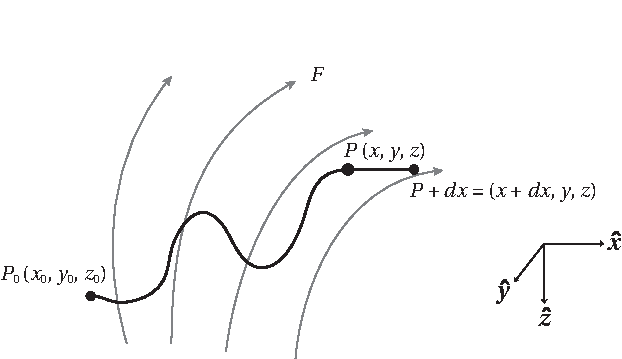
\includegraphics{potential/figures/work_path.pdf}
%     \caption{Path of a particle.}
%     \label{fig:path}
% \end{figure}

% Now lets suppose that we move our mass from $P_0$ starting at time $t_0$ and
% arrive at $P$ some time, $t$, later.  So lets integrate both sides with respect
% to time, which gives
% \begin{equation*}
%     \int_{t_0}^t \vb{F} \cdot \vb{v} \dd{t'} = K - K_0 .
% \end{equation*}
% We are going to do something a bit sneaky here and rewrite our integral in terms
% of space instead of time.  To do so, we need to change our limits of integration
% and our variable of integration.  We can relate the change in position
% $\dd{\vb{s}}$ to the change in time by $\dd{\vb{s}} = \vb{v} \dd{t'}$.  Just as velocity, 
% $\dd{\vb{s}}$ is a vector tangent to the path at all points.  This change in
% variables allows us to write
% \begin{equation*}
%     \int_{P_0}^P \vb{F} \cdot \dd{\vb{s}} = W(P,P_0) ,
% \end{equation*}
% where $W(P,P_0)$ is the work done in moving the mass from point $P_0$ to $P$.
% Note that we had to change from kinetic energy to work because our result is now
% independent of time.

% If the work done to move the test mass from $P_0$ to $P$ is independent of the
% path it takes to get the field is {\it conservative}.  While work is typically
% path-dependent, we will assume that for our purposes in this instance it is
% path-independent.  Lets add a third point a distance $\Delta x$ from $P$, $P +
% \Delta x$.  For a conservative field, the work done is path independent, hence,
% the work done moving from $P_0$ to $P$ and additionally from $P$ to $P + \Delta
% x$ must be the same as the work done in moving from $P_0$ to $P + \Delta x$,
% i.e.,
% \begin{equation*}
%     W(P,P_0) + W(P + \Delta x,P) = W(P + \Delta x,P_0) .
% \end{equation*}
% Our true interest is the incremental work required to move from $P$ to $P +
% \Delta x$, hence
% \begin{equation*}
%     W(P + \Delta x,P) = W(P + \Delta x,P_0) - W(P,P_0) .
% \end{equation*}
% Using our integral definition for a force we can write the above as
% \begin{equation*}
%     \int_{P}^{P + \Delta x} F_x(x,y,z) dx = W(P + \Delta x,P_0) - W(P,P_0) .
% \end{equation*}
% Dividing both sides by $\Delta x$ removes the integral.  According to the mean
% value theorem, mean of a function must fall on at least one point between the
% two end-points, which allows us to write the mean force in the $x$-direction as
% $F_x(x + \epsilon \Delta x,y,z)$ where $0 < \epsilon < 1$.  Hence,
% \begin{equation*}
%     F_x(x + \epsilon \Delta x,y,z) = \frac{W(P + \Delta x,P_0) - W(P,P_0)}{\Delta x} .
% \end{equation*}
% As $\Delta x \to 0$,
% \begin{equation*}
%     F_x(x,y,z) = \pdv{W}{x} .
% \end{equation*}
% If we apply the same logic to $y$- and $z$-directions, we find
% \begin{align*}
%     \vb{F}(x,y,z) & = \vu{x} \pdv{W}{x} + \vu{y} \pdv{W}{y} + \vu{z} \pdv{W}{z} ,\\
%     \vb{F} &= \grad W .
% \end{align*}

% Lets take this one step further.  Recall that a force is a scalar times a
% vector, $\vb{F} = m \vb{a}$, but lets make this general since we will not
% always discuss motion/gravity.  Sometimes we will be talking stresses in rocks (which
% act like springs), or forces on charged particles (electricity and magnetism).
% Therefore, lets instead write a force generally as a scalar constant, $b$, and a 
% vector field, $C$ (i.e., $\vb{F} = b \vb{C}$).  Let us then rewrite the result
% from our last step of our derivation above to give
% \begin{equation*}
%     b \vb{C} = b \grad (\phi) ,
% \end{equation*}
% where our work function $W$ is now written in terms of our generic scalar and a
% new scalar field, which we call the potential field, $\phi$.  We can now divide
% through by $b$ to achieve
% \begin{equation}
%     \vb{C} = \grad \phi .
% \end{equation}
\chapter{Diffusive Fields}\label{ch:diffusion}

\section{Introduction}

In the Chapter~\ref{ch:potential} we examined potential fields governed by Poisson's and Laplace's equations. These fields arise when conserved quantities are transported by gradient-driven fluxes under steady-state conditions, so that local sources are balanced by fluxes and no accumulation occurs. Gravity, magnetics, and steady-state heat conduction fall naturally into this class, and their behavior is dominated by global smoothness, scale separation, and nonuniqueness.

In this chapter, we relax the steady-state assumption. When fluxes are no longer instantaneously balanced by sources and sinks, conserved quantities are allowed to accumulate locally, and the system evolves in time. The result is diffusive behavior. Importantly, diffusion does not require new physics. The same conservation laws and constitutive relations introduced earlier still apply. What changes is the inclusion of storage.

Diffusion governs a wide range of geophysical processes, including transient heat flow, chemical transport, groundwater movement, electromagnetic induction, and even sediment transport.  These processes share a common mathematical structure despite their differing physical contexts. The diffusion equation describes how anomalies spread, weaken, and lose memory over time, introducing a natural time-length scale that is absent in steady-state potential fields.

Steady-state solutions are not discarded in this framework; rather, they emerge as the asymptotic limit of diffusion. Understanding diffusion therefore strengthens, rather than replaces, the interpretation of potential fields, and provides the foundation for time-dependent geophysical methods explored later in the course.

The goal of this chapter is to develop physical intuition for diffusive processes before focusing on specific applications. We will examine how conservation and constitutive laws combine to produce the diffusion equation, explore the physical meaning of its solutions, and highlight key differences between diffusive and steady-state behavior. These ideas will be revisited in subsequent chapters, where diffusion plays a central role in both electromagnetic and thermal problems.

\section{Time-dependent Conservation and Transport}

The defining distinction between steady-state potential fields and diffusive processes lies in whether conserved quantities are allowed to accumulate locally.  In Chapter~\ref{ch:potential}, we assumed steady state, so that sources and sinks were balanced by fluxes and no storage occurred. In diffusive systems, this restriction is lifted: imbalances between fluxes and sources lead to changes in storage over time.

Conservation requires that any change in the amount of a quantity stored within a region be explained by a balance between what enters, what leaves, and what is created or destroyed internally. If more of the quantity flows into a region than flows out, storage increases; if more flows out than in, storage decreases. Internal sources or sinks may add to or remove from this balance.

Described locally, conservation states that the rate of change of storage at a point reflects the combined effect of flux divergence and sources,
\[
    \pdv{\rho}{t} = -\div \vb{J} + s(\vb{x},t).
\]
where $\rho(\vb{x},t)$ denotes the density of the conserved quantity per unit volume. In contrast to the steady-state case, storage no longer remains constant, and its time dependence carries essential physical information. This time-dependent storage is what allows diffusive fields to evolve gradually rather than responding instantaneously. 

This expression states that changes in storage at a point arise from an imbalance between flux divergence and sources. In contrast to the steady-state case, the left-hand side is now nonzero and carries essential physical information.

\emph{Aside:} The steady-state case emerges naturally as a special limit of the time-dependent conservation law. Setting $\partial\rho/\partial t = 0$ recovers the steady-state conservation law introduced previously,
\[
    \div \vb{J} = s(\vb{x}),
\]
showing that steady-state fields represent a special balance condition within the more general time-dependent framework. Importantly, steady state does not imply zero flux; it implies that fluxes and sources are arranged so that storage does not change with time.

In the sections that follow, we combine this time-dependent conservation law with the same constitutive relations used for potential fields to obtain the diffusion equation. The resulting dynamics introduce characteristic time and length scales that fundamentally alter how geophysical fields evolve and how they can be interpreted.

\subsection{Constitutive Law for Diffusive Fluxes}

The inclusion of time dependence in the conservation law does not require a new description of how fluxes respond to spatial variations. As in the steady-state case, diffusive processes are governed by a local constitutive relation that links flux to the gradient of an intensive quantity. What changes between potential fields and diffusion is not the constitutive behavior, but the allowance for storage.

For many geophysical systems, flux arises in response to spatial gradients in a
scalar field $\phi(\vb{x},t)$,
\[
    \vb{J} = -k \grad \phi,
\]
where $\vb{J}$ is the flux of the conserved quantity, $\phi$ is the driving potential, and $k$ is a transport coefficient specific to the medium. The negative sign indicates that flux proceeds from regions of high potential toward regions of low potential.

This form encompasses a wide range of physical processes. In heat conduction, $\phi$ is temperature and $k$ is thermal conductivity. In chemical diffusion, $\phi$ is concentration and $k$ is the diffusivity multiplied by appropriate thermodynamic factors. In electromagnetics, $\phi$ may represent electric potential and $k$ corresponds to electrical conductivity. Despite the diversity of physical interpretations, the mathematical structure remains the same.

The constitutive relation above expresses two important assumptions. First, flux is a local response to the gradient of the potential; the flux at a point depends only on conditions in its immediate neighborhood. Second, the response is linear, so that doubling the gradient doubles the flux. These assumptions are well justified for many geophysical applications and allow the governing equations to be written in a form that is both physically transparent and mathematically tractable.

Because the constitutive law is unchanged from the steady-state case, diffusive behavior does not arise from a new transport mechanism. Instead, diffusion emerges from the interaction between this same gradient-driven flux and the time-dependent conservation of stored quantities. When gradients are allowed to persist in time, fluxes redistribute material, energy, or charge until balanced conditions are reached.

In the next section, we combine this constitutive relation with the time-dependent conservation law to obtain the diffusion equation and examine its physical meaning.

The detailed physical derivation of these relations is given in Box~\ref{box:diffusion}.

\ntextbox{Physical origin of the diffusion equation}{
    Diffusive fields arise from the same physical principles as steady-state potential
    fields: conservation of a quantity and a local relation between flux and spatial
    gradients. The difference is that storage is now allowed to vary in time.

    \medskip
    \noindent\textbf{Conservation with storage}\\
    Consider a fixed control volume $V$ bounded by a surface $\partial V$. Let
    $\rho(\vb{x},t)$ denote the density of a conserved quantity per unit volume,
    $\vb{J}(\vb{x},t)$ the associated flux, and $s(\vb{x},t)$ a volumetric source or
    sink. Conservation requires that the rate of change of the amount stored within $V$
    equal the net flux across the boundary plus internal sources,
    \[
        \dv{}{t}\int_V \rho\,\dd{V} =
        -\oint_{\partial V} \vb{J}\cdot\vb{n}\,\dd{S} + \int_V s\,\dd{V},
    \]
    where $\dd{S}$ denotes an element of surface area on the boundary of the control volume.
    Applying the divergence theorem and noting that the control volume is arbitrary
    yields the local conservation law,
    \[
        \pdv{\rho}{t} = -\div \vb{J} + s(\vb{x},t).
    \]
    In contrast to the steady-state case, the storage term
    $\partial\rho/\partial t$ is now nonzero and carries essential physical
    information.

    \medskip
    \noindent\textbf{Constitutive relation}\\
    As with potential fields, flux is assumed to respond locally and linearly to
    gradients in an intensive scalar quantity $\phi(\vb{x},t)$,
    \[
        \vb{J} = -k \grad \phi,
    \]
    where $k$ is a transport coefficient describing the efficiency of flux through the
    medium. This relation expresses locality and linear response and does not depend on
    whether the system is steady or time dependent.

    \medskip
    \noindent\textbf{Governing equation}\\
    Substituting the constitutive relation into the conservation law gives
    \[
        \pdv{\rho}{t} = \div\!\left(k \grad \phi\right) + s(\vb{x},t).
    \]
    This equation governs time-dependent, gradient-driven transport. To proceed further, storage must be related to the potential itself, which leads directly to the diffusion equation introduced in the main text.
}{core}\label{box:diffusion}


\section{Derivation of the diffusion equation}

Diffusive behavior emerges when a gradient-driven flux acts in concert with the time-dependent conservation of a stored quantity. No new physical assumptions are required beyond those already introduced.

We begin with the local conservation law for a conserved quantity,
\begin{equation}
    \pdv{\rho}{t} = -\div \vb{J} + s(\vb{x},t),
\end{equation}
where $\rho(\vb{x},t)$ is the stored quantity per unit volume, $\vb{J}$ is the flux, and $s(\vb{x},t)$ represents sources or sinks.

The constitutive relation describing diffusive transport relates flux to the gradient of a scalar potential,
\begin{equation}
    \vb{J} = -k \grad \phi,
\end{equation}
where $\phi(\vb{x},t)$ is the driving potential and $k$ is the transport coefficient.

Substituting the constitutive relation into the conservation law gives
\begin{equation}
    \pdv{\rho}{t} = \div\!\left(k \grad \phi\right) + s(\vb{x},t).
\end{equation}
This equation is the general form governing time-dependent, gradient-driven transport.  To proceed, we must relate storage $\rho$ to the potential $\phi$.

In many geophysical systems, changes in storage are proportional to changes in the potential,
\[
    \rho = c\,\phi,
\]
where $c$ is a storage coefficient that depends on material properties. For example, in heat conduction $c = \rho c_p$, while in chemical diffusion $c$ represents the concentration capacity of the medium.

Substituting this relation and assuming $c$ is constant yields
\begin{equation}
    c\,\pdv{\phi}{t} = \div\!\left(k \grad \phi\right) + s.
\end{equation}

If the transport coefficient $k$ is spatially uniform, this expression simplifies to
\begin{equation}
    c\,\pdv{\phi}{t} = k\,\laplacian \phi + s.
\end{equation}
Dividing through by $c$ gives
\begin{equation}
    \pdv{\phi}{t} = \kappa\,\laplacian \phi + \frac{s}{c},
    \label{eq:diffusion}
\end{equation}
where the diffusivity
\begin{equation}
    \kappa = \frac{k}{c}
\end{equation}
combines transport efficiency and storage into a single parameter.

Equation~\ref{eq:diffusion} is known as the \emph{diffusion equation}. It describes how the potential $\phi$ evolves in time as fluxes redistribute stored quantities in response to spatial gradients, leading to three clear insights.
\begin{enumerate}
    \item The rate at which potential changes is proportional to the spatial curvature of the field. Regions of high curvature (strong gradients in gradients) evolve most rapidly.

    \item The diffusivity constant controls the rate of evolution: higher diffusivity leads to faster redistribution and more rapid smoothing of the field.

    \item When the system evolves for long \emph{enough} that $\partial \phi / \partial t \to 0$, the system reaches steady state and the diffusion equation reduces to
    \[
        \laplacian \phi = -\frac{s}{k},
    \]
    the Poisson's equation! In the absence of sources, it further reduces to Laplace's equation. Steady-state potential fields therefore represent the long-time limit of diffusion.
\end{enumerate}

The diffusion equation is a parabolic partial differential equation, in contrast to the elliptic equations governing steady-state potential fields. This change in equation type reflects a fundamental shift in behavior: diffusion introduces finite rates of evolution, characteristic time scales, and memory of prior states.


\subsection{Physical interpretation of diffusivity}

The rate at which disturbances spread is controlled by a single combined parameter.  The diffusivity $\kappa$ sets the rate at which a diffusive disturbance spreads through space. It combines two competing effects: how efficiently flux is transmitted (through $k$) and how much of the quantity can be stored locally (through the storage term).

High diffusivity implies that gradients are rapidly smoothed and that disturbances propagate quickly. Low diffusivity implies slow redistribution and long-lived anomalies. For example, thermal diffusivity in rocks is small, so thermal anomalies persist over geological timescales, whereas electromagnetic diffusivity can be very large in resistive materials, allowing rapid penetration of transient fields (Table~\ref{tab:diffusivity}).
\begin{table}[htp]
    \centering
    \caption{Diffusivity and its relationship to transport efficiency, and storage in geophysical diffusion processes, $\kappa = k/c$.}
    \label{tab:diffusivity}
    \small
    \begin{tabularx}{\textwidth}{lYcYcYcc}
        \toprule
        \textbf{System} 
        & \textbf{Potential} 
        & $\phi$
        & \textbf{Transport efficiency} 
        & $k$
        & \textbf{Storage term} 
        & $c$
        & \textbf{Diffusivity} \\
        \midrule
        Heat conduction 
        & temperature & $T$ 
        & thermal conductivity & $k$ 
        & density \& specific heat capacity & $\rho C_P$ 
        & $\displaystyle \kappa = \frac{k}{\rho C_P}$ \\

        Chemical diffusion 
        & concentration & $C$ 
        & molecular diffusivity & $D$ 
        & $1$ (per unit concentration) &
        & $\displaystyle \kappa = D$ \\

        Groundwater flow 
        & hydraulic head & $h$ 
        & hydraulic conductivity & $K$ 
        & specific storage & $S_s$ 
        & $\displaystyle \kappa = \frac{K}{S_s}$ \\

        EM diffusion 
        & electric \& magnetic field & $E$, $H$
        & electrical conductivity & $\sigma$ 
        & magnetic permeability & $\mu$ 
        & $\displaystyle \kappa = \frac{1}{\mu\sigma}$ \\

        Fluid diffusion
        & velocity & $\vb{v}$ 
        & dynamic viscosity & $\mu$ 
        & mass density & $\rho$ 
        & $\displaystyle \kappa = \nu = \frac{\mu}{\rho}$ \\

        Sediment transport
        & elevation, sediment thickness & $h$
        & sediment mobility & $k_s$ 
        & effective density ($\phi$ = porosity) & $\rho_s(1 - \phi)$
        & $\displaystyle \kappa \sim \frac{k_s}{\rho_s(1 - \phi)}$ \\
        \bottomrule
    \end{tabularx}
\end{table}

Across all diffusive systems, the characteristic length--time relation
\[
    \ell \sim \sqrt{\kappa t}
\]
governs the spatial extent of influence after time $t$. Diffusivity therefore provides a direct link between observable time dependence and subsurface length scales.

\ntextbox{Units of Diffusivity}{
    \subsection{Why diffusivity has units of area per time}
    At first glance, the units of diffusivity, \si{m^2.s^{-1}} or equivalent, can appear counterintuitive. Diffusion occurs in three dimensions, so one might expect a volume-per-time quantity rather than an area-per-time quantity.

    The key point is that diffusivity does not describe the transport of volume; it describes the rate at which spatial gradients are smoothed. In the diffusion equation,
    \[
        \pdv{\phi}{t} = \kappa \laplacian \phi,
    \]
    the time derivative has units of $\phi$ per unit time, while the Laplacian has units of $\phi$ per unit length squared. Diffusivity therefore carries the units required to balance a second spatial derivative with a first time derivative.

    To put it more simply, diffusivity comes from combining transport efficiency and storage, $\kappa = k/c$. Using dimensional reasoning,
    the transport efficiency has units
    \[
	    \frac{\text{(flux)}}{\text{(gradient)}} \sim \frac{(\text{quantity}/\text{area}/\text{time})}{(\text{potential}/\text{length})}
    \]
    and the storage has units
	\[
        \frac{\text{quantity}}{\text{volume} \cdot \text{potential}}.
    \]
    Dividing them and everything cancels to $kappa \sim \frac{L^2}{T}$

    Physically, $\kappa$ sets the rate at which influence spreads laterally from a source. The square-root scaling $\ell \sim \sqrt{\kappa t}$ shows that diffusion naturally links time to a \emph{length squared}, not to a volume. Volume enters only indirectly through storage, which is already accounted for in the definition of $\kappa$.
}{core}\label{box:diff_units}

\section{Physical meaning of storage and diffusivity}

The time-dependent conservation law and constitutive relation introduce three quantities that control diffusive behavior: the storage variable $\rho$, the transport coefficient $k$, and the potential $\phi$. Although these symbols appear abstract, each has a clear physical meaning that depends on the system under consideration. Understanding these meanings is essential for interpreting the diffusion equation and its solutions.

\subsection{Storage: what accumulates}

The quantity $\rho(\vb{x},t)$ represents the density of the conserved quantity stored per unit volume. Storage determines how strongly a system responds to imbalances between fluxes and sources. When storage is large, changes occur slowly; when storage is small, the system responds rapidly.

Examples of storage include:
\begin{itemize}
    \item \textbf{Heat conduction}: $\rho$ represents thermal energy density, often
    written implicitly as $\rho c_p T$. Storage reflects the ability of a material
    to absorb heat without undergoing a large change in temperature.
    \item \textbf{Chemical diffusion}: $\rho$ corresponds to the concentration of a
    species. Storage reflects how much material can reside locally.
    \item \textbf{Groundwater flow}: $\rho$ represents fluid mass stored within pore
    space, controlled by porosity and compressibility.
    \item \textbf{Electromagnetic diffusion}: $\rho$ is associated with stored
    electromagnetic energy or charge density, depending on formulation.
\end{itemize}

In steady-state systems, storage does not change with time. In diffusive systems, storage evolves, providing the memory that allows the system to respond gradually rather than instantaneously.

\subsection{Potential: what drives the flux}

The scalar field $\phi(\vb{x},t)$ is the intensive quantity whose spatial gradients drive transport. It represents the local “level” of the system and determines the direction and magnitude of flux through its gradient.

Examples include:
\begin{itemize}
    \item Temperature in heat conduction
    \item Concentration in chemical diffusion
    \item Hydraulic head in groundwater flow
    \item Electric potential in electromagnetics
\end{itemize}

Although the physical meaning of $\phi$ varies, its mathematical role is always the same: differences in potential create gradients, and gradients produce flux.

\subsection{Transport coefficient and diffusivity}

The coefficient $k$ describes how efficiently the medium transmits flux in response to a gradient. It reflects material properties, connectivity, and microstructure.  High values of $k$ indicate that gradients are rapidly reduced by strong fluxes, whereas low values allow gradients to persist.

In many applications, it is useful to define a \emph{diffusivity},
\[
    \kappa = \frac{k}{\mathrm{storage}},
\]
which combines transport efficiency and storage into a single parameter with units of length squared per time. Diffusivity controls how quickly disturbances spread through a system.

A key and widely applicable scaling relation follows directly:
\[
    \ell \sim \sqrt{\kappa t},
\]
where $\ell$ is the characteristic distance over which a diffusive signal propagates in time $t$. This relationship highlights a central property of diffusion: spatial influence increases only with the square root of time.

\subsection{Why storage and diffusivity matter for interpretation}

Together, storage and diffusivity determine not only how fast a system evolves, but also how much information is preserved. Diffusive processes smooth spatial variations and progressively erase fine-scale structure. Early-time behavior is dominated by shallow or nearby features, while deeper or more distant structure emerges only at later times.

This behavior contrasts sharply with potential fields, which respond instantaneously to sources and lack an intrinsic time scale. Diffusion therefore introduces causality and temporal filtering, providing both challenges and opportunities for geophysical interpretation.

In the next section, we combine the time-dependent conservation law with the constitutive relation to obtain the diffusion equation and examine how these physical ideas are encoded mathematically.

\section{Diffusive Behavior: Spreading, Memory \& Timescales}

One of the most important and counterintuitive features of diffusive systems is how localized disturbances evolve in time. Consider an initial condition in which a conserved quantity is concentrated at a point or within a very small region.  Under diffusion, this localized excess does not propagate outward as a sharp front. Instead, it spreads smoothly, forming a Gaussian distribution whose width increases with time.

The impulse response of the diffusion equation illustrates these behaviours most clearly.
For a homogeneous medium with constant diffusivity $\kappa$ and no sources, the diffusion equation admits a fundamental solution corresponding to an initial impulse. In one spatial dimension, the solution for an initially localized disturbance takes the form
\[
    \phi(z,t) \propto \frac{1}{\sqrt{4\pi\kappa t}}
    \exp\!\left(-\frac{z^2}{4\kappa t}\right).
\]

Although the exact prefactor is not important for most physical interpretations, the shape of the solution is. The potential $\phi$ is Gaussian in space at any fixed time, and the characteristic depth (or length) of the distribution increases as
\[
    \ell \sim \sqrt{\kappa t}.
\]

As diffusion proceeds, the system progressively loses memory of initial conditions.  Gaussian spreading reflects the cumulative effect of many small, local fluxes acting over time. At early times, diffusion primarily redistributes material, energy, or charge over short distances. As time progresses, the influence of the initial disturbance extends farther, but increasingly weakly. The peak amplitude decreases as the distribution broadens, ensuring conservation of the total amount stored.

This behavior illustrates several defining features of diffusion:
\begin{itemize}
    \item Diffusion smooths spatial variations continuously rather than preserving
    sharp boundaries.
    \item The influence of a disturbance grows only as the square root of time,
    making diffusion intrinsically slow at large distances.
    \item Fine-scale structure is rapidly lost, while large-scale structure
    persists longer.
\end{itemize}

A subtle but important consequence of the diffusion equation is the absence of a finite propagation front.  Unlike wave propagation, diffusion has no finite propagation front. Any disturbance has an immediate, though vanishingly small, effect everywhere. This mathematical property reflects the local nature of diffusive fluxes and the absence of inertia.

\section{Physical meaning of diffusion}

The diffusion equation encodes several fundamental physical behaviors that distinguish diffusive systems from both steady-state potential fields and wave phenomena. These behaviors are independent of the specific physical context and apply equally to heat, chemical concentration, groundwater flow, and electromagnetic diffusion.

\subsection{Spreading and smoothing}

Diffusion continuously redistributes stored quantities from regions of high potential toward regions of low potential. As with potential fields, the solution can be viewed as a superposition of spatial waves that evolve over time,
\[
    \text{amplitude} \propto e^{ik\xi} e^{-k^2 \kappa t},
\]
where $k$ is the spatial frequency, $\xi$ is a spatial coordinate, and $\kappa$ is the diffusion coefficient.

Short wavelengths (large $k$) decay much more rapidly than long wavelengths. As a result, diffusion smooths and spreads structure at a rate controlled by $\kappa$: localized anomalies do not propagate as sharp features, but instead broaden and weaken over time. Spatial gradients are systematically reduced, and fine-scale structure is progressively erased.

This smoothing is irreversible: once sharp features have been diffused, they cannot be reconstructed without additional information. As a result, diffusion progressively erases high-frequency spatial information while preserving only large-scale trends.

\subsection{Memory loss}

Because diffusion involves both transport and storage, the system retains information about past conditions only for a finite time. Early in the evolution, the field reflects details of the initial or boundary conditions. As diffusion proceeds, these details are forgotten, and the system approaches a state governed primarily by sources, sinks, and boundary conditions.

In practical terms, diffusion acts as a temporal filter. Recent events leave a strong imprint, while older events become increasingly difficult to detect. This property is central to interpreting transient geophysical observations.

\subsection{Finite rates but infinite speed}

A mathematically subtle but important feature of diffusion is that disturbances affect the entire domain immediately: the diffusion equation permits nonzero responses at arbitrarily large distances for any $t > 0$. In this sense, diffusion has infinite propagation speed.

Physically, however, the influence of a disturbance at large distances is vanishingly small at early times. Diffusion operates through local fluxes driven by gradients, and information spreads gradually. There is no sharp front, no arrival time, and no transport of energy without accompanying loss of amplitude.

This behavior contrasts sharply with wave propagation, where finite speeds and distinct wavefronts carry information without immediate smoothing.

\subsection{Time--length scaling}

The combined effects of spreading and storage introduce a natural relationship between time and distance. For a diffusivity $\kappa$, the characteristic distance over which a diffusive signal spreads in time $t$ scales as
\[
    \ell \sim \sqrt{\kappa t}.
\]

This square-root scaling is one of the most important results in diffusion theory.  Doubling the distance influenced by diffusion requires four times as much time.  Consequently, diffusive processes are efficient at short distances and short times, but increasingly slow at transmitting information over large spatial scales.

This scaling governs the depth sensitivity of transient heat flow, electromagnetic induction, and chemical transport, and it underlies the distinction between early-time and late-time behavior discussed in the following sections.

\subsection{Why Gaussians are fundamental}

The Gaussian form is not an accident or a special case. It is the natural outcome of repeated local redistribution governed by the diffusion equation, and it serves as the building block for more complicated solutions. Arbitrary initial conditions can be viewed as superpositions of localized impulses, each of which spreads Gaussianly. As a result, Gaussian smoothing underlies the behavior of all diffusive processes.

Gaussian spreading explains why diffusive processes progressively erase high-frequency spatial information. Early-time observations are sensitive to near-surface or nearby structure, while deeper or more distant features emerge only after sufficient time has elapsed. This time-dependent filtering contrasts sharply with steady-state potential fields, which respond instantaneously and lack a characteristic timescale.

In later chapters, this same Gaussian spreading will reappear in the context of electromagnetic diffusion and transient heat flow, where time-dependent data can be exploited to probe structure as a function of depth.

\section{Canonical diffusive responses}

Although the diffusion equation can be solved numerically for arbitrary geometries and boundary conditions, a small number of canonical solutions provide most of the physical intuition needed for geophysical interpretation. These solutions describe idealized situations but serve as building blocks for understanding more complex cases.

\subsection{Impulse and point-source solutions}

One useful idealisation is a localized impulse input.  The impulse, or point-source, solution represents the response of a diffusive system to a localized, instantaneous input. As discussed previously, this response takes the form of a Gaussian that broadens with time. Because the diffusion equation is linear, arbitrary initial conditions can be represented as superpositions of such impulses. The evolution of any diffusive system can therefore be understood as the combined Gaussian spreading of its initial state.

\subsection{Step-change boundary conditions}

A second common class of solutions arises arises when a boundary condition changes abruptly. For example, if the temperature at the surface is suddenly raised and held fixed, the resulting thermal perturbation diffuses downward over time. The solution in this case involves the error function, which describes how the influence of the boundary propagates into the medium.

Physically, this solution emphasizes that diffusion transmits information from boundaries as well as from internal sources. The depth to which a surface disturbance has penetrated after time $t$ is again controlled by the diffusive length scale $\sqrt{\kappa t}$.

\subsection{Sinusoidal forcing}

Periodic or sinusoidal boundary conditions—such as seasonal variations in surface temperature or oscillatory electromagnetic fields—produce solutions in which amplitude decays exponentially with depth while phase lags increase downward.  These solutions are particularly important in geophysics because they allow depth to be inferred from frequency-dependent attenuation and phase shift.

Despite their differing forms, all canonical solutions of the diffusion equation share the same underlying behavior: smoothing of spatial gradients, progressive loss of high-frequency structure, and evolution governed by the diffusivity.

\section{Early-time and late-time behavior}

Time dependence introduces a natural ordering to diffusive responses. The information contained in a diffusive signal depends strongly on when it is observed relative to the characteristic diffusion time scale.

At early times, diffusive disturbances remain localized near their origin.  Gradients are steep, fluxes are strong, and the effects of boundaries or distant structure have not yet propagated to the observation point. As a result, early-time signals are dominated by shallow or nearby features.

From a practical standpoint, early-time diffusion carries the highest spatial resolution, but the weakest signal amplitudes. This makes early-time observations both valuable and challenging: they are information-rich but sensitive to noise and modeling assumptions.

At late times, diffusion has redistributed the conserved quantity over larger distances. Gradients are weaker, amplitudes are reduced, and the influence of deeper or more distant structure becomes apparent. Eventually, the system approaches steady state, and the temporal evolution slows markedly.

Late-time behavior is less sensitive to fine-scale structure but more robust to noise. In the long-time limit, the diffusion equation reduces to the steady-state potential problem described in Chapter~\ref{ch:potential}.

The distinction between early and late times illustrates a fundamental tradeoff in diffusive systems: resolution versus stability. Early times emphasize local detail, while late times emphasize large-scale structure. Effective interpretation therefore requires careful consideration of the time window being examined.

\section{Diffusion Versus Wave Propagation}

Diffusion and wave propagation represent two fundamentally different modes of transport in physical systems. Although both are described by partial differential equations, their mathematical character and physical implications are markedly distinct.

The diffusion equation is parabolic, reflecting the dominance of storage and gradient-driven flux. Disturbances spread gradually, amplitudes decrease with time, and spatial detail is irreversibly smoothed. Diffusion has no finite propagation speed; any disturbance affects the entire domain immediately, but with rapidly diminishing strength at large distances.

By contrast, the wave equation is hyperbolic and arises when inertia or restoring forces dominate over dissipative effects. Wave propagation involves finite speeds, sharp wavefronts, and oscillatory solutions. Energy can propagate without immediate loss of structure, allowing travel times, reflections, and resonances to be observed.

These differences have profound consequences for geophysical interpretation.  Diffusive methods emphasize amplitude decay, phase lag, and temporal smoothing, whereas wave-based methods exploit arrival times, interference, and impedance contrasts. Diffusion tends to erase information as time progresses, while waves can preserve it over long distances.

Together with steady-state potential fields, diffusion and wave propagation form three complementary classes of geophysical behavior:
\begin{itemize}
    \item Potential fields: instantaneous, global sensitivity, no intrinsic time
    scale
    \item Diffusive fields: time-dependent smoothing with characteristic
    time--length scaling
    \item Wave fields: finite-speed propagation with preserved structure
\end{itemize}

Understanding which regime applies—and when one transitions into another—is central to interpreting geophysical observations and selecting appropriate methods.

\section{Diffusion in geophysical systems}

Diffusion is not a specialized process confined to thermal physics or chemistry; it is one of the fundamental ways in which the Earth redistributes energy, mass, and charge. In geophysics, diffusion governs how anomalies evolve, how information is transmitted through the subsurface, and how depth sensitivity emerges from time-dependent observations.

What makes diffusion particularly important is not merely its ubiquity, but its interpretational consequences. Diffusive systems smooth spatial structure, lose memory of initial conditions, and introduce intrinsic time and length scales that are absent in steady-state potential fields.

Heat transport in the Earth is fundamentally diffusive. Short-term variations in surface temperature propagate downward over time, while long-term thermal structure reflects the balance between internal heat production and boundary conditions. Because thermal diffusivity is small, diffusion filters high-frequency signals rapidly, leaving only long-wavelength, long-timescale information at depth.

As a result, geothermics is most sensitive to large-scale thermal structure and integrated heat budgets rather than fine-scale heterogeneity. Steady-state heat flow represents the long-time limit of thermal diffusion, while transient methods can probe shallower structure and recent thermal history.

Time-varying electromagnetic fields in the Earth are governed by diffusion rather than wave propagation over most geophysical frequencies. Electrical conductivity controls the rate at which induced currents diffuse, producing characteristic amplitude decay and phase lag with time and depth.

This diffusive behavior underlies methods such as transient electromagnetics and magnetotellurics, where frequency or time serves as a proxy for depth. Early-time or high-frequency signals respond to shallow structure, while late-time or low-frequency signals sample deeper regions. The square-root time--length scaling introduced earlier directly controls this depth sensitivity.

Fluid flow and solute transport in the subsurface also exhibit diffusive behavior when driven by hydraulic gradients or concentration differences. Storage in pore space and compressibility introduces time dependence, while permeability and diffusivity control the rate of redistribution.

In these systems, early-time responses emphasize local structure and hydraulic connectivity, while late-time behavior reflects regional flow patterns and boundary conditions. Diffusion therefore governs both the evolution of contaminant plumes and the recovery of aquifers.

\subsection{What diffusion reveals—and what it hides}

From an interpretational standpoint, diffusion presents both opportunities and limitations. Time dependence allows additional information to be extracted that is unavailable from steady-state observations. However, diffusion also destroys spatial detail, making inverse problems increasingly ill-posed at late times.

This tradeoff mirrors that encountered with potential fields: diffusion distributes information broadly but smooths it irreversibly. Effective geophysical interpretation therefore depends on selecting appropriate time or frequency ranges to balance resolution and stability.

\section{Summary and Forward Connections}

Together with steady-state potential fields and wave propagation, diffusion completes the triad of fundamental field behaviors in geophysics:
\begin{itemize}
    \item Potential fields describe instantaneous balance without intrinsic time
    scales.
    \item Diffusion introduces time dependence, memory loss, and characteristic
    depth penetration.
    \item Wave propagation preserves structure through finite-speed transport and
    interference.
\end{itemize}

Understanding diffusion provides the conceptual bridge between static and dynamic geophysical methods. The ideas developed in this chapter reappear throughout the course, particularly in electromagnetic methods and in the interpretation of transient signals across a wide range of geophysical applications.
\chapter{Wave Fields}\label{ch:waves}

\section{Introduction}

In the previous Chapters~\ref{ch:potential} and \ref{ch:diffusion} we examined potential fields and diffusive fields, which describe how conserved quantities respond to spatial gradients under distinct assumptions about time. Potential fields arise when sources and fluxes are in instantaneous balance, while diffusive fields emerge when storage allows systems to evolve gradually toward equilibrium. Both classes redistribute structure smoothly and do not exhibit finite propagation speeds.

In this chapter we introduce a third and fundamentally different mode of behavior: wave propagation. Wave fields arise when conserved quantities are coupled to both restoring forces and inertia. Under these conditions, disturbances propagate at finite speeds, transport energy through the medium, and preserve structured information in time.

The wave equation governs a wide range of geophysical phenomena. These include seismic waves in solids, acoustic waves in fluids, electromagnetic waves (e.g., ground-penetrating radar), thermal waves driven by periodic forcing (e.g., climate and seasonal heat signals), and fluid waves associated with pressure and free-surface motion. Despite their differing physical origins, all wave phenomena share a common mathematical structure and a set of characteristic behaviors.

Unlike potential fields and diffusion, wave propagation does not inherently smooth spatial structure. Instead, waves transmit signals through the medium, often with attenuation and dispersion that depend on material properties. Finite travel times, reflections at boundaries, refraction due to spatial heterogeneity, diffraction around obstacles, and interference between waveforms are common features of all wave fields.

From a geophysical perspective, waves are uniquely powerful because they preserve spatial and temporal structure during propagation. Information is encoded in arrival times, amplitudes, phases, and waveforms rather than in static or time-averaged fields. As a result, wave-based observations form the foundation of seismology, radar methods, and many active-source and time-dependent imaging techniques.

The goal of this chapter is to develop physical intuition for wave behavior independent of any specific application. We examine how conservation laws, restoring forces, and inertia combine to produce the wave equation, explore the properties of wave solutions, and contrast wave propagation with the diffusive and steady-state behaviors encountered previously. These ideas provide the conceptual basis for seismic, electromagnetic, and fluid-wave methods developed later in the course.

\section{From conservation to wave motion}

Wave propagation emerges when conservation laws operate in the presence of both restoring forces and inertia. As in potential and diffusive fields, conservation of a physical quantity remains central. What distinguishes wave behavior is that the system resists motion through inertia and is driven back toward equilibrium by restoring forces rather than by diffusive smoothing.

To see this, consider a medium that can be displaced from equilibrium. A local disturbance produces a restoring force that acts to reverse the displacement. At the same time, inertia prevents the system from responding instantaneously. The resulting competition between restoring forces and inertia allows disturbances to propagate through the medium as waves.

From a conservation perspective, wave motion is most naturally associated with the conservation of momentum or energy rather than the direct conservation of a scalar quantity such as mass or heat. A local force imbalance leads to acceleration, not immediate transport or storage. This distinction is fundamental: in diffusion, imbalances drive fluxes that redistribute stored quantities, whereas in waves, imbalances drive motion that transports energy through the medium.

Restoring forces take different physical forms in different systems. In elastic solids, they arise from stress-strain relationships; in fluids, from pressure gradients; in electromagnetic waves, from the coupling between electric and magnetic fields. In all cases, the restoring force acts to oppose displacement from equilibrium.

Inertia provides the second essential ingredient. Without inertia, restoring forces would lead only to instantaneous relaxation, as in diffusion. Inertial resistance causes the system to overshoot equilibrium, producing oscillatory behavior. These oscillations allow energy to be transmitted through the medium rather than locally dissipated.

The presence of inertia introduces finite propagation speeds and causality. A disturbance at one location influences another only after sufficient time has elapsed for the wave to travel between them. This behavior stands in sharp contrast to both potential fields, which respond instantaneously, and diffusive fields, which respond everywhere immediately but only weakly at large distances.

Viewed in this light, wave propagation represents a third fundamental response to imbalance in physical systems:
\begin{itemize}
    \item potential fields enforce instantaneous balance,
    \item diffusion relaxes imbalance through gradual redistribution and storage,
    \item waves transport imbalance through oscillatory motion and energy flow.
\end{itemize}

In the next section, we make these ideas concrete by deriving the wave equation and examining how restoring forces and inertia combine to determine propagation speed and wave behavior.

\section{The wave equation}

The discussion in the previous section identified restoring forces and inertia as the essential ingredients required for wave propagation. When these ingredients are combined with conservation principles, the result is a governing equation that describes the propagation of disturbances through a medium at finite speed.

To illustrate this structure, we first consider a simplified case in which wave motion can be described by a single scalar field $\phi(\vb{x},t)$. This scalar form of the wave equation captures the essential physics common to many wave phenomena, including acoustic waves, electromagnetic waves in homogeneous media, and simplified elastic motion. More complex wave systems encountered in geophysics—particularly seismic waves in solids—require a vector or tensor description and are addressed separately.

The physical origin of the wave equation is presented in Box~\ref{box:wave_derivation}.  Here we summarize the key result.

When inertia resists acceleration and restoring forces act to oppose displacement, the evolution of the field $\phi$ is governed by
\[
    \pdv[2]{\phi}{t} = c^2 \laplacian \phi,
\]
where $c$ is the wave speed. This equation describes the propagation of disturbances without intrinsic smoothing or storage-driven relaxation. Instead, energy is transported through the medium by oscillatory motion.

The appearance of a second-order time derivative distinguishes wave propagation from diffusion. In diffusive systems, storage leads to gradual relaxation toward equilibrium, whereas in wave systems inertia allows disturbances to overshoot equilibrium and propagate. The resulting motion preserves structure over time and enforces causality through finite propagation speed.

\subsection{Scope and limitations}

The scalar wave equation provides a useful conceptual framework, but it does not capture the full richness of wave phenomena in elastic solids. In particular, seismic waves involve vector displacement fields and tensor relations between stress and strain. These lead to multiple wave modes, including compressional (P) waves, shear (S) waves, and surface waves, each with distinct propagation characteristics.

Rather than introduce this complexity here, we use the scalar wave equation to develop intuition for wave behavior common to all wave fields. The full elastic wave equation and the resulting diversity of seismic wave types are developed in detail in the seismology chapter.

\ntextbox{Physical origin of the wave equation}{
    Wave propagation arises from the interaction between inertia and restoring forces.  This can be illustrated using a simple one--dimensional medium in which a scalar field $\phi(x,t)$ describes displacement from equilibrium.

    \medskip
    \noindent\textbf{Inertia} \\
    A small element of the medium resists changes in motion according to Newton's second law. The inertial response is proportional to the second time derivative of the displacement,
    \[
        \text{force per unit volume} \;\propto\; \pdv[2]{\phi}{t}.
    \]

    \medskip
    \noindent\textbf{Restoring force}\\
    Displacement from equilibrium produces a restoring force that tends to return the system to its original state. For small deformations, this restoring force is proportional to spatial curvature in the displacement,
    \[
        \text{restoring force per unit volume} \;\propto\; \laplacian \phi.
    \]

    \medskip
    \noindent\textbf{Balance of forces}\\
    Equating inertial and restoring terms leads to
    \[
        \pdv[2]{\phi}{t} = c^2 \laplacian \phi,
    \]
    where the wave speed $c$ depends on the ratio of the restoring stiffness of the medium to its inertial mass density.

    \medskip
    \noindent This equation describes the propagation of disturbances at finite speed without diffusive smoothing. Energy is conserved locally and transported through the medium by oscillatory motion.
}{core}\label{box:wave_derivation}

\section{Finite propagation speed and wave velocity}

A fundamental distinction between wave fields and both potential and diffusive fields is the existence of a finite propagation speed. Disturbances do not influence the entire domain instantaneously; instead, information and energy travel through the medium at a characteristic velocity determined by material properties.

Wave velocity arises from the balance between restoring forces and inertia. Strong restoring forces increase wave speed, while larger inertia slows propagation. This relationship is general: regardless of the physical nature of the wave, velocity reflects the ratio of stiffness to mass or storage.

The parameter $c$ has units of velocity and represents the speed at which disturbances propagate (Table~\ref{tab:velocity}). Unlike diffusivity, wave speed does not introduce smoothing. Ideal wave solutions preserve waveform shape during propagation.
\begin{table}[bth]
    \centering
    \caption{Wave velocity in common geophysical and geoscientific systems}
    \label{tab:wave_velocity}
    \begin{tabularx}{\textwidth}{lXYX}
        \toprule
        \textbf{System} &
        \textbf{Wave type} &
        \textbf{Velocity expression} &
        \textbf{Controlling properties} \\
        \midrule
        Elastic solids
        & Seismic body waves
        & $c \sim \sqrt{\mathrm{elastic modulus}/\rho}$
        & Bulk/shear modulus, density \\

        Elastic solids
        & Seismic surface waves
        & $c \lesssim c_S$
        & Near-surface structure, layering \\

        Fluids
        & Acoustic waves
        & $c = \sqrt{K/\rho}$
        & Bulk modulus, density \\

        Electromagnetics
        & EM waves (GPR, radar)
        & $c = 1/\sqrt{\mu\varepsilon}$
        & Permeability, permittivity \\

        Thermal systems
        & Thermal waves
        & $c_{\mathrm{phase}} = \omega/k$
        & Diffusivity, forcing frequency \\

        Fluid surfaces
        & Gravity waves
        & $c \sim \sqrt{g\lambda}$
        & Gravity, wavelength \\

        Porous media
        & Pressure waves
        & $c \sim \sqrt{K_{\mathrm{eff}}/\rho_{\mathrm{eff}}}$
        & Frame rigidity, fluid coupling \\
        \bottomrule
    \end{tabularx}
\end{table}

Finite propagation speed introduces causality. A point in space responds to a disturbance only after sufficient time has elapsed for the wave to travel from the source. Travel times, arrival sequences, and waveform evolution therefore carry direct information about the medium through which the wave has passed.


\section{General properties of wave propagation}

Solutions of the wave equation exhibit a set of characteristic behaviors that are common to all wave phenomena, regardless of their physical origin.  The wave equation admits a rich set of solutions that describe how disturbances interact with material boundaries, propagate through heterogeneous media, and transport energy. These properties arise directly from the combination of restoring forces and inertia and distinguish wave fields from both steady-state potential fields and diffusive systems.  Although the physical interpretation of waves varies across geophysics, the same mathematical relationships govern their behavior. In this section we introduce a set of general concepts and equations that apply broadly to seismic, acoustic, electromagnetic, thermal, and fluid waves.

\subsection{Impedance and wave interaction with boundaries}

A central quantity in wave propagation is the \emph{wave impedance}, which measures how a medium resists motion or field oscillation. Impedance combines inertial and restoring properties and depends on the physical system. For a wide class of scalar waves, it may be written schematically as
\[
    Z = \frac{\text{restoring strength}}{\text{particle or field velocity}}.
\]

At a boundary separating two media, impedance controls how wave energy is partitioned between reflection and transmission. For normally incident waves, the amplitude reflection and transmission coefficients can be written in the general form
\[
    R = \frac{Z_2 - Z_1}{Z_2 + Z_1}, \qquad
    T = \frac{2 Z_2}{Z_1 + Z_2},
\]
where $Z_1$ and $Z_2$ are the impedances of the incident and transmitted media, respectively. These expressions apply to acoustic waves, electromagnetic waves, and elastic waves under appropriate definitions of impedance.

Large impedance contrasts lead to strong reflections, while small contrasts favor transmission. This simple result underlies reflection seismology, radar sensing, and many scattering phenomena.

In systems where multiple wave modes are possible—most notably in elastic solids—incident wave energy can be partitioned among reflected and transmitted modes with different polarizations and speeds. While the scalar wave equation does not capture this behavior, the underlying principles of impedance contrast and slowness conservation remain valid. The detailed treatment of mode conversion is reserved for the seismology chapter.

\subsection{Reflection and refraction: Snell's law}

When waves encounter a planar interface at an angle, their directions of propagation change in a way constrained by phase continuity along the boundary.  This requirement leads to Snell's law, which relates angles of incidence, reflection, and transmission (Figure~\ref{fig:wave_phenomena}).
\begin{figure}[bth]
    \centering
    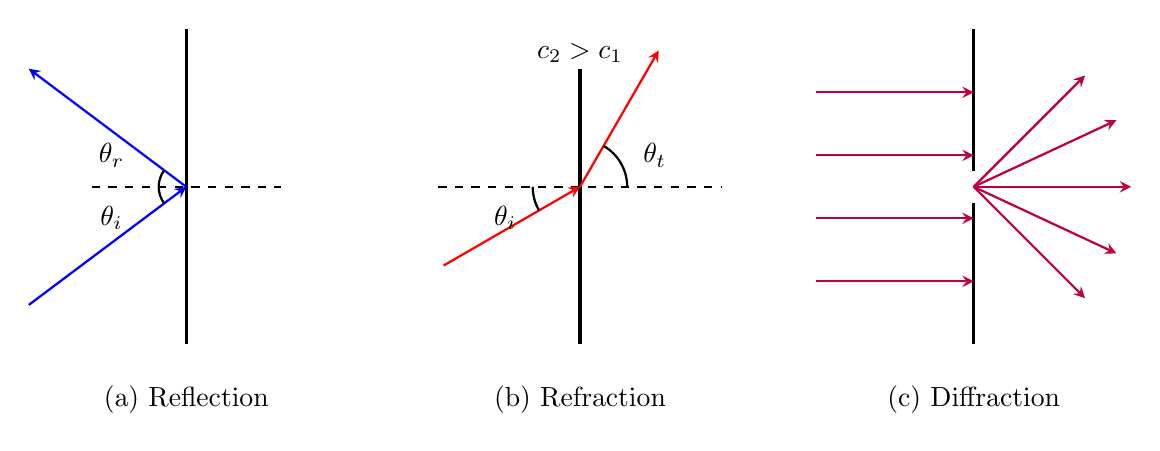
\begin{tikzpicture}[scale=1.0, thick, >=stealth]

    %========================
    % Panel (a): Reflection
    %========================
    \begin{scope}[shift={(0,0)}]
        % Boundary
        \draw[very thick] (0,0) -- (0,4);
        %\node[rotate=90] at (-0.45,2) {Boundary};

        % Normal
        \draw[dashed] (-1.2,2.0) -- (1.2,2.0);
        %\node at (1.35,2.5) {Normal};

        % Incident wave
        \draw[->, blue] (-2,0.5) -- (0,2.0);
        %\node[blue] at (-1.6,1.2) {Incident};

        % Reflected wave
        \draw[->, blue] (0,2.0) -- (-2,3.5);
        %\node[blue] at (-1.6,3.7) {Reflected};

        % Angles
        \draw (-0.35,2.0) arc[start angle=180,end angle=217,radius=0.35];
        \node at (-0.95,1.6) {$\theta_i$};

        \draw (-0.35,2.0) arc[start angle=180,end angle=143,radius=0.35];
        \node at (-0.95,2.4) {$\theta_r$};

        % Label
        \node at (0,-0.7) {(a) Reflection};
    \end{scope}

    %========================
    % Panel (b): Refraction (explicit angles)
    %========================
    \begin{scope}[shift={(5,0)}]

        % Interface (vertical)
        \draw[very thick] (0,0) -- (0,3.5);

        % Normal (horizontal, pointing to the right)
        \draw[dashed] (-1.8,2) -- (1.8,2);
        %\node at (2.0,2) {Normal};

        % Incident ray: -30° from normal
        % Direction = 180 - 30 = 150 degrees
        \draw[<-, red] (0,2) -- ++(210:2);
        %\node[red] at (-1.7,2.7) {Incident};

        % Transmitted ray: +60° from normal
        % Direction = 0 + 60 = 60 degrees
        \draw[->, red] (0,2) -- ++(60:2);
        %\node[red] at (1.6,3.2) {Refracted};

        % Incident angle theta_i (between normal and incident ray)
        \draw (-0.6,2)
            arc[start angle=180,end angle=210,radius=0.6];
        \node at (-0.95,1.6) {$\theta_i$};

        % Transmitted angle theta_t (between normal and refracted ray)
        \draw (0.6,2)
            arc[start angle=0,end angle=60,radius=0.6];
        \node at (0.95,2.4) {$\theta_t$};

        % velocity labels
        \node at (0,3.7) {$c_2 > c_1$};

        % Panel label
        \node at (0,-0.7) {(b) Refraction};

    \end{scope}

    %========================
    % Panel (c): Diffraction
    %========================
    \begin{scope}[shift={(10,0)}]
        % Barrier with aperture
        \draw[very thick] (0,0) -- (0,1.8);
        \draw[very thick] (0,2.2) -- (0,4);
        %\node[rotate=90] at (-0.45,2) {Barrier};

        % Incident waves
        \foreach \y in {0.8,1.6,2.4,3.2} {
            \draw[->, purple] (-2,\y) -- (0,\y);
        }
        %\node[purple] at (-1.6,0.5) {Incident};

        % Diffracted waves
        \foreach \angle in {-45,-25,0,25,45} {
            \draw[->, purple] (0,2) -- ++(\angle:2);
        }
        %\node[purple] at (1.7,3.5) {Diffracted};

        % Label
        \node at (0,-0.7) {(c) Diffraction};
    \end{scope}

    \end{tikzpicture}
    \caption{Schematic illustration of (a) reflection, (b) refraction, and (c) diffraction of waves.  Dashed lines indicate the surface normal relevant to Snell's law.  Geometry is schematic and not to scale.}
    \label{fig:wave_phenomena}
\end{figure}

For reflection, the angle of incidence equals the angle of reflection, both
measured from the surface normal,
\[
    \theta_i = \theta_r .
\]

For transmission (refraction), the angles are related by
\[
    \frac{\sin \theta_i}{c_1} = \frac{\sin \theta_t}{c_2},
\]
where $c_1$ and $c_2$ are the wave speeds in the two media. This form emphasizes that refraction arises from changes in propagation speed, not from changes in frequency.

A more general and widely transferable form of Snell's law expresses conservation of horizontal slowness,
\[
p = \frac{\sin \theta}{c},
\]
which remains constant across interfaces. This formulation applies equally to seismic, acoustic, and electromagnetic waves and provides a natural bridge to ray theory and travel-time analysis developed later.

\subsection{Diffraction and wavelength effects}

Waves also exhibit diffraction: the tendency to spread laterally when encountering obstacles or apertures comparable in size to the wavelength. Diffraction places a fundamental limit on spatial resolution and ensures that wave energy is not confined to perfectly sharp paths.

As a result, wave behavior depends not only on geometry and boundaries, but also on the relationship between wavelength and the scale of heterogeneity in the medium.  This scale dependence will reappear when discussing the resolving power of wave-based geophysical methods.

\subsection{Superposition and interference}

The wave equation is linear, which allows solutions to be superposed. When multiple waves occupy the same region of space, their displacements add. This superposition can produce constructive and destructive interference, giving rise to complex spatial and temporal patterns even in simple media.

Interference underlies many familiar wave phenomena, including beat patterns, standing waves, and resonances. In geophysics, interference plays an important role in shaping observed waveforms and spectra.


\section{Energy transport, attenuation, and dispersion}

Waves transport energy through a medium rather than redistributing it locally, but real geophysical materials do not transmit energy without loss or modification. As waves propagate, their amplitudes and frequency content evolve due to a combination of geometric effects, intrinsic dissipation, and scattering.

\subsection{Attenuation and Spherical Spreading}
In an ideal, lossless medium, the wave equation conserves energy. Energy is carried by the oscillatory motion of the medium or field and propagates at the group velocity. This transport allows waves to convey structured information over long distances without intrinsic smoothing, in contrast to diffusion.  The energy flux associated with a wave is proportional to the square of its amplitude, which makes amplitude a sensitive carrier of information about the propagation environment (Box~\ref{box:information}).

Ideal wave equations conserve energy, but real materials dissipate it. Attenuation describes the loss of wave amplitude due to intrinsic dissipation (e.g., viscosity, anelasticity, electrical resistance) and scattering. A common mathematical representation of attenuation is an exponential decay with distance,
\[
    A(x) = A_0\, e^{-\alpha x},
\]
where $\alpha$ is the attenuation coefficient. Attenuation reduces amplitudes but does not intrinsically alter propagation speed.

It is important to distinguish attenuation from diffusion. Diffusion irreversibly smooths structure, whereas attenuation reduces amplitude while preserving waveform shape over short distances.

Even in the absence of attenuation, wave amplitudes decrease as energy spreads over increasing area or volume. For point sources in three dimensions, spherical spreading leads to
\[
    A(r) \propto \frac{1}{r},
\]
while cylindrical spreading leads to $A(r) \propto r^{-1/2}$. Geometric spreading is a purely kinematic effect and applies to all wave types.

\subsection{Dispersion, Phase and Group Velocity}
A medium is dispersive if wave speed depends on frequency. In dispersive systems, different frequency components of a signal propagate at different velocities, causing waveforms to change shape with distance.  Dispersion is described through the relationship between angular frequency $\omega$ and wavenumber $k$. The phase and group velocities,
\[
    c_p = \frac{\omega}{k}, \qquad c_g = \frac{d\omega}{dk},
\]
may differ substantially in dispersive media.

The phase velocity $c_p$ describes the speed of constant phase (e.g., wave crests), while the group velocity $c_g$ describes the speed at which energy and information propagate.  The distinction between phase and group velocity is essential for interpreting wave packets, dispersion, and frequency-dependent travel times. These ideas will reappear in later chapters in the context of seismic surface waves, guided waves, and electromagnetic propagation.

Dispersion plays a critical role in surface waves, guided waves, electromagnetic propagation in layered media, and thermal or diffusive “wave-like” responses under periodic forcing.

\ntextbox{Memory and information in diffusive and wave systems}{
    When we describe diffusive and wave systems as having different degrees of memory or information content, we are not using metaphorical language. We are describing how much of a system's past or spatial structure remains encoded in observable signals as they propagate through a medium.

    \medskip
    \noindent\textbf{Memory in diffusive systems}\\
    Diffusive systems possess limited and rapidly degrading memory. Information about an initial disturbance is retained only transiently and only in a highly smoothed, integrated form. As diffusion proceeds, local gradients relax, and fine-scale structure is irreversibly erased.  In practical terms, this means that a diffusive signal carries information primarily about:
    \begin{itemize}
        \item the gross distribution of sources and boundaries,
        \item the integrated properties of the medium,
        \item and the time elapsed since perturbation.
    \end{itemize}

    Early-time diffusive responses may retain some sensitivity to local structure, but this sensitivity decays rapidly. At late times, different initial conditions that share similar large-scale properties become indistinguishable. Diffusion therefore acts as both a spatial and temporal low-pass filter, progressively losing information about the detailed path taken by energy, mass, or charge.  This behavior is why diffusive methods emphasize bulk properties and why inverse problems based on diffusion are strongly non-unique and increasingly ill-posed at late times.

    \medskip
    \noindent\textbf{Memory and information in wave systems}\\
    Wave systems behave fundamentally differently. Because waves propagate via oscillatory motion rather than gradual relaxation, they preserve structured information as they travel. This information is not stored locally but is carried by the wave itself.  In geophysics, information about the medium and the propagation path is encoded in multiple observable attributes of a wavefield, including:

    \begin{itemize}
        \item travel times, which reflect integrated velocity along the propagation path;
        \item relative arrival times of different phases, which constrain structure and layering;
        \item amplitude, which reflects geometrical spreading, attenuation, and impedance contrasts;
        \item phase and polarity, which encode boundary interactions and mode conversions;
        \item wavelet shape and frequency content, which reflect dispersion and attenuation; and
        \item coda length and complexity, which record scattering and multipathing. 
    \end{itemize}

    A key point is that this information is path-dependent. As a wave travels, it is continually modified by the material it encounters, and these modifications accumulate coherently rather than being smoothed away. In this sense, a wavefield retains a memory of its history: the source wavelet is convolved with the impulse response of the Earth along each propagation path.  This is why waves are so powerful for imaging. Even a single waveform can contain multiple, overlapping pieces of information about source location, medium structure, and boundary geometry.

    \medskip
    \noindent\textbf{Causality and information transport}\\
    The difference in memory between diffusive and wave systems is closely tied to causality.
    
    Diffusive systems respond everywhere immediately, but only weakly at large distances. Information spreads, but without a sharp arrival time or a clear causal sequence.
    
    Wave systems exhibit finite propagation speed. Information arrives at distinct times, in ordered sequences, allowing causal interpretation: one feature happened before another.  This temporal ordering is essential for extracting directional and geometric information, such as travel paths, reflectors, and interfaces.

    \medskip
    \noindent\textbf{Why this distinction matters in geophysics}\\
    Understanding memory and information content clarifies why different geophysical methods are suited to different questions.

    Diffusion-based observations are best for estimating bulk properties, long-term evolution, and integrated structures.  Wave-based observations are best for recovering geometry, layering, and localized heterogeneity.

    Neither is “better” in an absolute sense—they answer different questions because they retain different kinds of information.
}{aside}\label{box:information}


\section{Potential, diffusive, and wave fields: a unified perspective}
With the introduction of wave propagation, we can now place potential fields, diffusive fields, and wave fields within a single conceptual framework. All three arise from conservation laws combined with constitutive relations, but they differ in the physical mechanisms through which imbalance is resolved.

Potential fields (elliptic) phenomena enforce instantaneous balance between sources and fluxes. They exhibit global sensitivity, intrinsic smoothness, and strong non-uniqueness, with no characteristic time scale.

Diffusive fields (parabolic) resolve imbalance through gradual redistribution and storage. They introduce memory loss, smoothing, and a characteristic time-length scale $\ell \sim \sqrt{\kappa t}$. In the long-time limit, the diffusive field approaches elliptic behavior.

Wave fields (hyperbolic) resolve imbalance through oscillatory motion mediated by inertia and restoring forces. They exhibit finite propagation speed, preserve structured information, and transport energy through the medium.  The wave equation also differs in that it does not admit a steady-state or diffusive limit: energy propagates rather than relaxes.

These distinctions reflect differences in mathematical character rather than differences in conservation principles.

The three field types also differ fundamentally in how information is encoded and transmitted:
\begin{itemize}
    \item potential fields integrate information globally and do not encode causal ordering;
    \item diffusive fields partially retain information at early times but progressively forget it; while
    \item wave fields preserve path-dependent, time-ordered information in amplitudes, phases, and waveforms.
\end{itemize}
This hierarchy explains why different geophysical methods are sensitive to different aspects of subsurface structure and why combining methods can reduce ambiguity.

The essential differences can be summarized schematically:
\begin{align*}
    \laplacian{\phi} &= s && \text{(potential fields)} \\
    \pdv{\phi}{t} &= \kappa \laplacian{\phi} && \text{(diffusion)} \\
    \pdv[2]{\phi}{t} &= c^2 \laplacian{\phi} && \text{(waves)}
\end{align*}
The progression from elliptic to parabolic to hyperbolic equations reflects increasing dynamical complexity and increasing information retention.

\section{Connection to geophysics}
Wave propagation is central to many geophysical and geoscientific methods, precisely because waves preserve information about structure, geometry, and material properties along their propagation paths.
In the Earth, wave phenomena arise in many contexts:
\begin{itemize}
    \item seismic waves in elastic solids,
    \item acoustic waves in fluids and the atmosphere,
    \item electromagnetic waves used in radar and remote sensing,
    \item periodic temperature changes at Earth's surface or at the base of the oceans,
    \item surface and gravity waves in oceans and rivers,
    \item pressure waves in porous and fractured media.
\end{itemize}

Although these systems involve different physical variables, they share common governing principles and mathematical structure.

\subsection{Imaging and inference}
Wave-based methods excel at resolving geometry. Travel times constrain velocity and layer thickness, amplitudes reveal impedance contrasts and attenuation, and waveform shapes encode dispersion and scattering. Reflections, refractions, and diffractions provide complementary constraints on boundaries and heterogeneities.

Because waves retain memory of their propagation history, inverse problems based on wave data are typically better constrained than those based solely on potential or diffusive fields, though they remain computationally challenging.

\subsection{Relationship to later chapters}
The scalar wave equation and general properties introduced here provide the foundation for later chapters on seismology, radar methods, and electromagnetic wave propagation. In those chapters, the simplified framework developed here will be extended to include: vector and tensor fields, multiple wave modes, mode conversion and anisotropy, frequency-dependent attenuation and dispersion.

By establishing the common physics of wave propagation early, later method-specific developments can focus on interpretation rather than rederiving fundamental concepts.

Together with potential and diffusive fields, wave fields complete the triad of fundamental geophysical responses to imbalance. Understanding how and why these different field types behave as they do is essential for selecting appropriate methods, interpreting observations, and integrating multiple datasets into coherent models of the Earth.


\part{Geophysical Fields and Methods}
% Potential fields (mostly)
\chapter{Gravity}\label{ch:gravity}

\epigraph{ ``Why are things so heavy in the future?  Is there a problem with the Earth's gravitational pull?''}
{{\normalfont ---\ Dr Emmett Brown}, Back to the Future}

\section{Introduction}

Gravity is the first geophysical method introduced in this course, and it serves as the archetype for all potential-field methods that follow. Gravity measurements sense variations in the Earth's gravitational acceleration produced by lateral contrasts in mass density. Unlike geothermics, gravity does not measure a state variable, nor does it involve time dependence or propagation. The gravity field responds instantaneously to the present-day distribution of mass and therefore contains no intrinsic memory of geological history. What gravity offers instead is a direct window into how geometry and density combine to shape an observable field.

From a geophysical perspective, gravity is fundamentally an integrative method. Every mass contrast within the Earth contributes to the measured signal, and the observed gravity anomaly represents the superposition of contributions from structures at all depths and scales. Nearby and shallow sources tend to dominate short-wavelength features, while deeper and more extensive structures control long-wavelength trends. As a result, gravity is exceptionally sensitive to geometry—depth, thickness, lateral extent, and shape—often more so than to the precise value of density itself. Understanding how geometry controls anomaly form is therefore central to gravity interpretation.

Gravity is also the clearest setting in which to confront non-uniqueness. Many different mass distributions can produce indistinguishable gravity anomalies, and no gravity dataset alone can uniquely determine subsurface structure. Interpretation necessarily proceeds by constructing forward models, applying geological constraints, and asking what classes of models are consistent with the observations. Rather than a limitation of the method, this non-uniqueness is a defining feature of potential fields and motivates the careful use of simplified source models, assumptions, and corrections.

In this chapter, gravity is developed as a steady-state potential field governed by Newtonian gravitation and Poisson's equation. We emphasize the principle of superposition, the role of canonical source geometries, and the connection between density variations and Earth structure and composition. Gravity provides the first opportunity in the course to see how simple models, forward calculations, and geological reasoning combine to extract physically meaningful constraints from inherently ambiguous data. These ideas will recur throughout the remaining geophysical methods and form the conceptual foundation for inversion and computational approaches introduced later.

Gravity — Revised Planning Outline
Framing \& motivation

Gravity as the archetypal potential field
What gravity measures and what it does not

Key ideas

Superposition
- Geometry dominance
- Non-uniqueness
- Steady-state behaviour

Physical basis
- Newtonian gravitation
- Potential, field, Poisson's equation

Superposition and building anomalies
- From bodies to geology
- Additivity as the organizing principle

Canonical source models
- Sphere
- Infinite cylinder (2D)
- Infinite slab
- Point mass (conceptual)

Density of Earth materials
- Minerals → rocks → porosity
- Revisiting mixing laws

Corrections as geological assumptions
- What is removed
- What is assumed

Forward modeling paradigms
- Talwani (2D)
- Pixel / voxel models
- Vertical columns
- Equivalent sources

Non-uniqueness and interpretation
- Equivalence
- Limits of gravity alone

Looking Ahead
- Magnetics
- Inversion
- Isostasy (as separate chapter)

\ntextbox{Key Concepts}{
\begin{itemize}
    \item \textbf{Gravity measures a force field produced by mass contrasts, not a state variable.}

    Gravity observations reflect the present-day distribution of mass density and contain no intrinsic time dependence or memory of geologoical history.

    \textit{How does this distinguish gravity from methods that measure state variables (e.g., temperature) or time-dependent signals (e.g., waves)?}

    \item \textbf{Gravity anomalies arise through superposition of contributions from all mass contrasts.}

    Every density contrast within the Earth contributes additively to the observed field, making superposition the organizing principle for both interpretation and modeling.

    \textit{How can complex geological structures be decomposed into simpler components for forward modeling?}

    \item \textbf{Geometry controls gravity signals more strongly than precise density values.}

    Depth, thickness, lateral extent, and shape exert first-order control on anomaly amplitude and wavelength, often dominating over uncertainty in density itself.

    \textit{Which geometric parameters most strongly influence the observable gravity field?}

    \item \textbf{Gravity is a steady-state, instantaneous field with no intrinsic memory.}

    The gravity field responds immediately to changes in mass distribution and contains no information about the timing or history of geological processes.

    \textit{What kinds of geological questions are therefore inaccessible to gravity alone?}

    \item \textbf{Gravity is inherently non-unique.}

    Many different mass distributions can produce indistinguishable gravity anomalies, and gravity data alone cannot uniquely determine subsurface structure.

    \textit{What additional geological or geophysical constraints are required to reduce ambiguity?}

    \item \textbf{Canonical source models are deliberate abstractions that build intuition and constrain interpretation.}

    Simple bodies such as spheres, cylinders, and slabs are not realistic representations of geology, but they reveal scaling behavior, depth sensitivity, and bounding limits on plausible structures when the appropriate abstraction is chosen.

    \textit{How can an oversimplified model still provide meaningful constraints on real Earth structure?}

    \item \textbf{Analytic gravity models provide benchmarks for numerical forward and inverse methods.}

    Numerical codes should be able to reproduce analytic solutions within expected tolerance; failure to do so indicates problems with implementation rather than geology.

    \textit{Why are benchmark tests essential before interpreting results from complex numerical models?}

    \item \textbf{Density variations reflect Earth structure and composition.}

    Variations in mineralogy, lithology, porosity, pressure, and temperature give rise to density contrasts that underpin gravity anomalies.

    \textit{How do compositional and structural factors translate into observable density contrasts?}

    \item \textbf{Gravity corrections encode geological assumptions.}

    Latitude, free-air, Bouguer, terrain, and related corrections are not purely technical adjustments but reflect specific assumptions about reference structures and mass distributions.

    \textit{How do different correction choices change the geological meaning of a gravity anomaly?}

    \item \textbf{Gravity interpretation relies on forward modeling rather than direct inversion.}

    Interpretation proceeds by proposing models, computing their gravity response, and assessing consistency with observations rather than by recovering a unique solution.

    \textit{How does forward modeling shape the way gravity data are interpreted compared to imaging methods?}
\end{itemize}
}{core}
% \begin{itemize}
%     \item How do the force of gravity, the gravitational attraction, and the
%     gravitational potential relate to one another? 

%     \item How do we determine the gravitational attraction due to an object?

%     \item What corrections must be applied to gravity data?

%     \item What gives rise to variations in density?
% \end{itemize}

\section{Mathematical symbols and units}
\begin{table}[hbt]
    \caption{Definitions of symbols.\vspace{2pt}}
    \label{tab:gravsym}
    \begin{tabular*}{\textwidth}{@{}cll@{}}
        \toprule
        Symbol &
        Quantity &
        SI Unit \\
        \midrule
        $x$, $y$, $z$   & distance                      & meter, m \\
        $r$             & radius                        & meter, m \\
        $m$             & mass                          & kilogram, kg \\
        $V$             & volume                        & m$^{3}$ \\
        $\rho$          & mass density                  & kg~m$^{-3}$ \\
        $\vb{F}$      & force                         & newton, N = kg~m~s$^{-2}$ \\
        $U$             & gravitational potential       & joule, J = N~m \\
        $\vb{g}$      & gravitational acceleration    & m~s$^{-2}$ \\
        $G$             & gravitational constant        & $6.6725985 \times
            10^{-11}$m$^{3}$~kg$^{-1}$~s$^{-2}$ \\
        %$\lambda$       & wavelength                    & m \\
        %$k$             & wavenumber ($k = 2\pi \lambda^{-1}$)
        %    & radians m$^{-1}$ \\
        \bottomrule
    \end{tabular*}
\end{table}

The standard SI units of gravitational acceleration are m~s$^{-2}$, where 1~m~s$^{-2}$ is equivalent to 10$^2$~cm~s$^{-2}$ in the cgs system.  We also call the cgs unit the Gal (sometimes gal, after Galileo).  For geophysics, the changes that we seek are often much smaller than a Gal.  So we commonly use the mGal ({\it milli}-Gal, 10$^{-5}$~m~s$^{-2}$) and $\mu$Gal ({\it micro}-Gal, 10$^{-8}$~m~s$^{-2}$).


\section{Theory}
In this section, we will cover the derivation of the gravitational attraction from the gravitational potential due to a uniform distribution of mass.  The goal is to develop a relationship that we can use to model gravity for a known geometry.  While we want ultimately want gravity, it is easier to work with the scalar potential than gravity, a vector quantity.  So the general procedure is to find the potential using superposition of small volumes of equal density and add them up---integrate over volume---and then find the gradient in the potential---take the derivative.

The Newtonian law of universal gravitation state that the magnitude of force due to gravity is proportional to the product of the masses and the inverse square of the distance between them,
\begin{equation}
    \vb{F} = G \frac{m m_0}{r^2} \vu{r}.
\end{equation}
A $\vu{r}$ is added to indicate that the force acts in a line defined by the centers of the two masses.  In addition, we must add a constant, $G$, to make the units work out properly since Newton's formulation is actually a proportionality.  The distance between the two masses, $r$, is determined by their relative positions in space.  If we place one mass at $P$ located at $(x,y,z)$ and a second at $P'$ located at $(x',y',z')$, the distance between the two masses is given by the Pythagorean theorem:
\begin{equation}
    r = [(x - x')^2 + (y - y')^2 + (z - z')^2]^{1/2}
\end{equation}
(Fig.~\ref{fig:twomass}).  The direction of the line between the centers is determined by the differences between the components,
\begin{equation}
    \vu{r} = \frac{1}{r}[(x - x')\vu{x} + (y - y')\vu{y} + (z -
    z')\vu{z}] .
\end{equation}
In order to make $\vu{r}$ a unit vector, we must divide by $r$.  By our definition above, we have defined the origin centered about $P'$.
\begin{figure}[hbt]
    \centering
    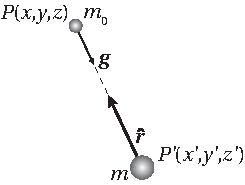
\includegraphics[]{gravity/figures/two_masses2.pdf}
    \caption{Two masses, one of interest $m$ located at $P'$ and the second a test mass, $m_0$, located at our point of observation $P$.  The unit vector is defined outwards from the center of mass, $m$, while the gravitational attraction, $\vb{g}$, at point $P$ due to $m$ is positive towards the center of mass $m$.}
    \label{fig:twomass}
\end{figure}

Above, we have described the relationship between masses and the gravitational attraction.  How can we use this relationship to investigate Earth?  As it stands, it is difficult from just this relationship since it depends on two masses: the mass of interest, $m$, and a mass that we use to measure the force, $m_0$.  But suppose we use multiple instruments to measure mass---Earth is pretty big as you know.  This requires that all $m_0$'s are identical so that the value of the force would be the same for each instrument.  A better approach would be looking for a field which does not require a test mass.

Newton's second law of motion, defines a force as $\vb{F} = m\vb{a}$, where $\vb{a}$ is an acceleration.  If we assume our mass is a test mass
\footnote{We will use the term test mass to indicate a small mass at our point of interest.  A test mass is a place holder within an equation and cancels out of derivations so its exact magnitude is irrelevant.  We will use a similar term to describe poles and charges in future chapters.},
$m_0$, and change the designation of acceleration from $\vb{a}$ to $\vb{g}$, we can write
\begin{equation*}
    \vb{F} = m_0 \vb{g} .
\end{equation*}
Equating the two equations above, we can solve for the acceleration due to
gravity,
\begin{equation}
    \vb{g}(P) = - G \frac{m}{r^2} \vu{r}.
\end{equation}
This result above is {\it fantastic} as it allows us to measure a field that will be the same regardless of the test mass we choose to determine it.  Note: the addition of the minus sign is a matter of convention and indicates that the force points away from our test mass, $m_0$, and in the direction of the mass, $m$.

We also want to get rid of the vector, at least for the moment, as keeping track of vector components can be quite tedious.  Since gravity is a potential field, we can relate the vector gravitational attraction to a scalar gravitational potential, $U$, by
\begin{equation}
    \vb{g}(P) = \grad U(P) .
    \label{eq:gpotential}
\end{equation}
To find the potential from the gravitational attraction,
\begin{align*}
    U(P) &= \int_{\infty}^{P} \vb{g} \cdot \vu{dr}' \\
        &= - G \int_{\infty}^{P} \frac{m}{r'}\vu{r}' \cdot \vu{dr}' \\
        &= -G \Bigg. \frac{m}{r} \Bigg|_\infty^P = G \frac{m}{r} .
\end{align*}

If we wanted to use the equation above to determine the gravitational potential we could do so by employing the principle of superposition,
\begin{equation*}
    U = G \sum_i \frac{m_i}{r_i} .
\end{equation*}
However, can you imagine doing so for an object the the size of Earth?  Even a tiny crystal has so many individual atoms (point masses) that it would be impractical to compute $\vb{g}$ from so many sources.  But there is another, simpler way to employ the principle of superposition assuming the distribution of masses is relatively constant throughout the medium (Fig.~\ref{fig:massdensity}).  We can express this mass distribution as a mass density, $\rho$, in terms of the elemental mass, $\dd{m}$, per elemental volume, $\dd{v}$,
\begin{equation*}
    \dd{m} = \rho \, \dd{v} .
\end{equation*}
Inputting this relationship into the gravitational potential, we find
\begin{equation}
    U(P) = G \int_V \frac{\rho(P')}{r}\, \dd{v} .
    \label{eq:gpot}
\end{equation}
Once we estimate the potential, we simply take the gradient to determine the gravitational attraction as indicated by Eq.~\ref{eq:gpotential},
\begin{equation*}
    \vb{g}(P) = - G \int_V \frac{\rho(P')}{r^2} \vu{r}\, \dd{v} .
\end{equation*}
Assuming mass is constant throughout the body, we can rewrite the above result as
\begin{equation}
    \vb{g}(P) = - G \rho \int_V \frac{\vu{r}}{r^2} \, \dd{v} .
\end{equation}

\begin{figure}[hbt]
    \centering
    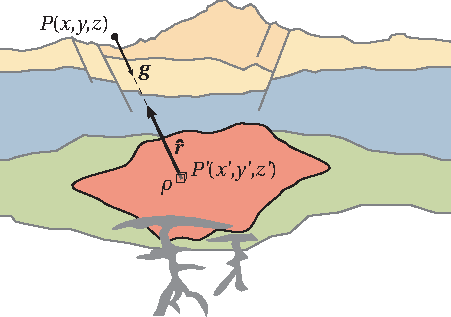
\includegraphics[]{gravity/figures/density.pdf}
    \caption{Instead of adding up each mass, we can describe a body of uniform mass distribution (density, $\rho$) and integrate over volume to determine the gravitational attraction due to the body.}
    \label{fig:massdensity}
\end{figure}

This result provides us with a simpler way to determine the gravitational attraction.  First determine $U$, then differentiate to find $\vb{g}$.

Traditionally gravimeters only measured the vertical component of gravity $g_z$, which was referenced to the geoid (local horizontal as measured by a spirit level).  This method is still the most commonly applied for exploration; hence, we only need to take the vertical derivative of the potential (i.e., $g_z = -\pdv{U}{z}$) for many applications.  The vertical component is given by
\begin{align}
    g_z &= - G \rho \int_z\int_y\int_x \frac{(z - z')}{r^3}\, \dd{x}\,\dd{y}\,\dd{z} &&
    \text{Cartesian} \\
    &= - G \rho \int_z\int_r\int_\phi \frac{(z - z')}{r^2}\, \dd{\phi}\,\dd{r}\,\dd{z} &&
    \text{cylindrical} \\
    &= - G \rho \int_r\int_\theta\int_\phi \sin \theta \cos \theta\,
    \dd{\phi}\,\dd{\theta}\,\dd{r} &&
    \text{spherical},
\end{align}
for each of the commonly used coordinate systems.  These relationships are used to estimate observed gravity from an assumed set of mass distributions.


\section{Gravity Anomalies}
Now that we have a way to determine the potential due to a mass distribution, lets look at some.  Consider a body of uniform density sitting in a half space with a different uniform density.  We will also make an important change in the way we estimate gravity here.  Instead of discussing absolute density, we will describe our bodies of interest in terms of either a mass excess or deficit (i.e. the difference in density between the body of interest and the medium; Fig.~\ref{fig:ds}).  We do this because for the same density contrast, the background gravitational attraction is uniformly increased or decreased by the value of the medium.  However, our measurements are relative which means that we can never be quite sure what the background attraction should be.
\begin{figure}[h]
    \centering
    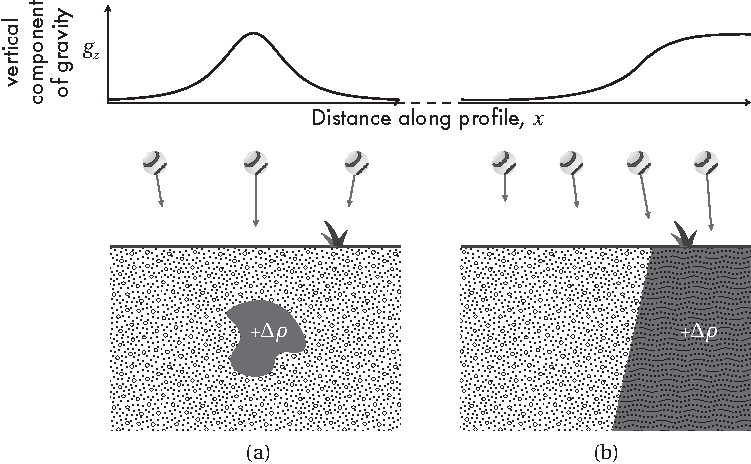
\includegraphics[]{gravity/figures/density_sensitivity.pdf}
    \caption{The gravitational attraction, $\vb{g}$, is changes in response to
    local density variations.}
    \label{fig:ds}
\end{figure}

In the derivations that follow, we will derive the gravity anomalies (or potential) due to several simple geometric objects: a buried sphere; an infinite slab of finite thickness; etc.  You may ask why we do such simple derivations when geologic objects have very complex shapes.  But to first order, geologic structures can approximated by these simple shapes, or perhaps a combination of a few.  For example, diapir shaped intrusions can be approximated as spheres and sedimentary layers or an aquifer can be approximated by the infinite slab. 

\subsection{Spherical Shell}
One of the simplest objects that we can compute the gravitational potential for is a sphere (Figure~\ref{fig:ss}).  While the solution is straightforward and can easily determine the solution without a laborious integration, we will derive the result instead to illustrate how to illustrate the process of computing potential.

Consider a sphere with uniform density, $\rho$, and radius, $a$.  We wish to determine the gravitational attraction due to this sphere at an observation point, $P$, a distance, $R$, from the center of the sphere.  To find the potential, we use Equation~\ref{eq:gpot},
\begin{equation*}
    U(R) = -G \rho \int_V \frac{\dd{v}}{D},
\end{equation*}
where $D$ is the distance to each volume element, $\dd{v}$.  The distance from $P$ to $\dd{v}$ is given by,
\begin{equation*}
    D = (R^2 + r^2 - 2 R r \cos \theta)^{1/2},
\end{equation*} 
where $r$ is the radius of a spherical shell within the sphere.  In spherical coordinates, we can write the each volume element as $\dd{v} = r^2 \sin \theta \,\dd{r} \dd{\theta} \dd{\phi}$.  We want to add up the individual potentials from each volume element.
\begin{figure}
    \centering
    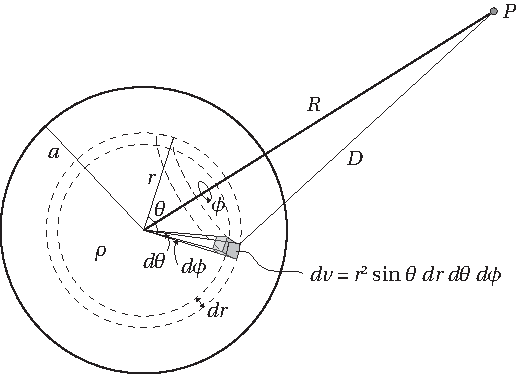
\includegraphics[]{gravity/figures/spherical_shell.pdf}
    \caption{Description of symbols for a spherical shell.}
    \label{fig:ss}
\end{figure}

To do this, we need to integrate over each of the three coordinates:
\begin{align*}
    U(R) &= -G \rho \int_0^a \dd{r} \int_0^\pi \dd{\theta} \int_0^{2\pi} \frac{r^2
        \sin \theta}{(R^2 + r^2 - 2 R r \cos \theta)^{1/2}} \dd{\phi} \\
    &= -2 \pi G \rho \int_0^a \dd{r} \int_0^\pi
        \frac{r^2 \sin \theta}{(R^2 + r^2 - 2 R r \cos \theta)^{1/2}} \dd{\theta} .
\end{align*}
Integrating over $\theta$ is a bit annoying but we can show
\begin{equation*}
    D \,\dd{D} = R r \sin \theta \,\dd{\theta} ,
\end{equation*}
which simplifies our integral considerably,
\begin{align*}
    U(R) &= -2 \pi G \rho \int_0^a \dd{r} \int_{D_{\mathrm{min}} 
        = R - r}^{D_{\mathrm{max}} = R + r} \frac{r}{R} \dd{D} \\
    &= -2 \pi G \rho \int_0^a \frac{r}{R} \Bigg. D \Bigg|_{R - r}^{R + r} \dd{r} \\
    &= -2 \pi G \rho \int_0^a \frac{r}{R} [R + r - (R - r)] \dd{r} \\
    &= -4 \pi G \rho \int_0^a \frac{r^2}{R} \dd{r} .
\end{align*}
Our final step is to then take the integral over $r$,
\begin{align*}
    U(R) &= -\frac{4}{3} \pi G \rho \Bigg. \frac{r^3}{R} \Bigg|_0^a \\
    &= -\frac{4}{3} \pi G \rho \frac{a^3}{R} .
\end{align*}

We will leave the derivation of the gravitational attraction to the problem set.

\subsection{Infinite Slab}
Consider a circular slab of finite extent (we will get to the infinite part later) with a radius of $R$, thickness, $h$, and a uniform density distribution, $\rho$ (Figure~\ref{fig:slab}).  We wish to find the vertical component of gravity, $g_z$, due to this slab at point, $P$, at a distance $b$ above the surface.  Starting with the general gravitational potential, equation \ref{eq:gpot},
\begin{equation*}
    U(P) = -G \rho \int_V \frac{\dd{v}}{D} .
\end{equation*}
We will perform the integration over the volume of the infinite slab in cylindrical coordinates to exploit symmetry and convenience of the system that are more difficult to do in a Cartesian reference frame.
\begin{figure}[bthp]
  \centering
  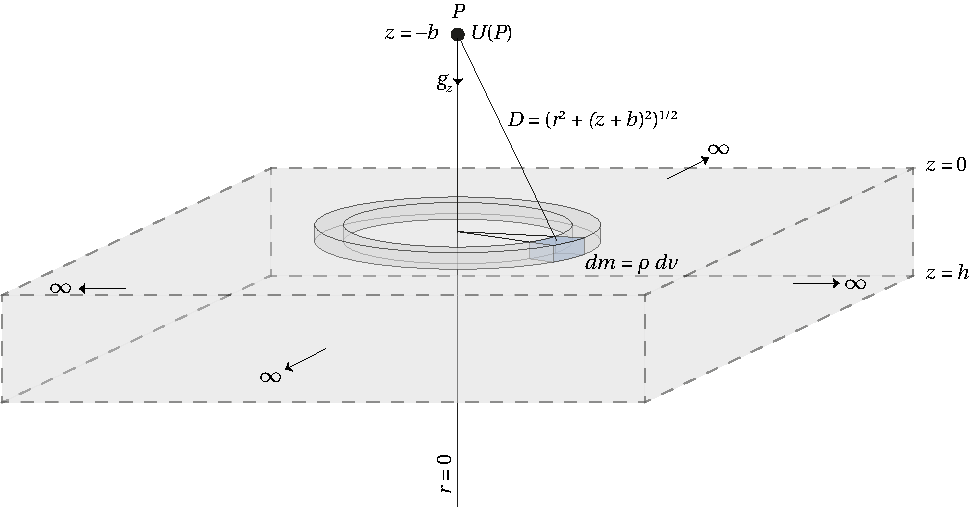
\includegraphics[width=\textwidth]{gravity/figures/infinite_slab.pdf}
  \caption{An infinite slab with thickness, $h$, and density, $\rho$.  Our observation point, $P$, sits a distance $b$ above the surface.  Each infinitesimally small volume, $dv$, has a mass, $dm = \rho dv$.  Note: as is often the case with geophysics, we have defined the $z$-axis as positive down.  Also defining the top of the slab to be at $z=0$ results in a negative value for the height above the surface.}
  \label{fig:slab}
\end{figure}

Sitting at an observation point above the slab, we will integrate over the volume of the slab by integrating infinitesimally small segments around a cylindrical rings and starting from the axis moving away and from the top to the bottom of the slab (Figure~\ref{fig:slab} and \ref{fig:dv}.
\begin{figure}[bthp]
  \centering
  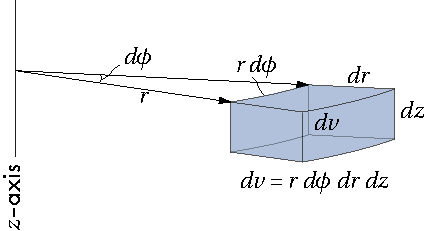
\includegraphics{gravity/figures/volume_element.pdf}
  \caption{A volume element as defined by the cylindrical coordinate system.}
  \label{fig:slab}
\end{figure}
First though, we need to write our potential in cylindrical coordinates.  A volume element in cylindrical coordinates is defined as $\dd{v} = r \dd{\phi} \dd{r} \dd{z}$.  The distance from the observation point to the volume element, $D = (r^2 + (z + b)^2)$.  Hence, the potential in cylindrical coordinates is given by
\begin{equation*}
    U = -G \rho \int_0^h \int_0^R \int_0^{2\pi}
    \frac{r \dd{\phi} \dd{r} \dd{z}}{(r^2 + (z + b)^2)^{1/2}}
\end{equation*}
Note: even though this is an infinite slab, we will perform the integration for a slab of finite radius $R$ and later discuss the implications as $R \to \infty$.  To find the gravitational acceleration, we need to take the gradient of potential.  We are only interested in the vertical component of gravity, so
\begin{equation*}
    \pdv{}{z} U(D) = \pdv{}{z} \left[ -G \rho \int_0^h \int_0^R \int_0^{2\pi}
    \frac{r \dd{\phi} \dd{r} \dd{z}}{(r^2 + (z + b)^2)^{1/2}} \right]
\end{equation*}
Since only the denominator of the fraction within the integral has a z-term, all other components can be assumed constants during integration, i.e.,
\begin{equation*}
    g_z = \pdv{}{z} U = -G \rho \int_0^h \int_0^R \int_0^{2\pi} r \dd{\phi}
    \dd{r} \dd{z} \pdv{}{z} \frac{1}{(r^2 + (z + b)^2)^{1/2}} .
\end{equation*}

Evaluating the derivative, we find
\begin{align*}
    \pdv{}{z} \frac{1}{(r^2 + (z + b)^2)^{1/2}}
    &= -\frac{1}{2} 2 (z + b) \frac{1}{(r^2 + (z + b)^2)^{3/2}} \\
    &= -\frac{(z + b)}{(r^2 + (z + b)^2)^{3/2}} .
\end{align*}
Inserting this result back into the vertical gravitational acceleration above,
\begin{equation*}
    g_z = -G \rho \int_0^h \int_0^R \int_0^{2\pi} 
    \frac{(x + b) r \dd{\phi} \dd{r} \dd{z}}{(r^2 + (z + b)^2)^{3/2}} .
\end{equation*}
Integrating around the cylindrical ring (over $\phi$) is easy since there are no
$\phi$'s in our expression and can all be assume constant.  The integral we are
performing is
\begin{align*}
    \int_0^{2\pi} \dd{\phi} &= \bigl. \phi \bigr|_0^{2\pi} \\
    &= 2\pi - 0 = 2\pi .
\end{align*}
Inserting this result into our equation above,
\begin{equation*}
    g_z = -2 \pi G \rho \int_0^h \int_0^R
    \frac{(x + b) r \dd{r} \dd{z}}{(r^2 + (z + b)^2)^{3/2}} .
\end{equation*}
Next, we perform the integration over $r$ from the axis out to the edge of the
slab,
\begin{align*}
    \int_0^R \frac{(x + b) r \dd{r}}{(r^2 + (z + b)^2)^{3/2}} 
    &= \left.  \frac{-(z + b)}{(r^2 + (z + b)^2)^{1/2}} \right|_0^R. \\
    &= -\frac{(z + b)}{(R^2 + (z + b)^2)^{1/2}} + \frac{(z + b)}{((z + b)^2)^{1/2}} \\
    &= -\frac{(z + b)}{(R^2 + (z + b)^2)^{1/2}} + \frac{(z + b)}{((z + b)} \\
    &= -\frac{(z + b)}{(R^2 + (z + b)^2)^{1/2}} + 1 .
\end{align*}
Inserting this result into $g_z$, we find,
\begin{equation*}
    g_z = -2 \pi G \rho \int_0^h \int_0^R
    \left[ 1 - \frac{(z + b)}{(R^2 + (z + b)^2)^{1/2}} \right] \dd{z} .
\end{equation*}
We need to perform one last to integration to derive the gravitation due to a slab with finite extent,
\begin{align*}
    \int_0^h \left[ 1 - \frac{(z + b)}{(R^2 + (z + b)^2)^{1/2}} \right] \dd{z} 
    &= \int_0^h dz - \int_0^h \frac{(z + b)}{(R^2 + (z + b)^2)^{1/2}} \dd{z} \\
    &= \bigl. z \bigr|_0^h + \bigl. (R^2 + (z + b)^2)^{1/2} \bigr|_0^h \\
    &= h + (R^2 + (h + b)^2)^{1/2} - (R^2 + b^2)^{1/2} .
\end{align*}
Inserting this result, we arrive at
\begin{equation}
    g_z = -2 \pi G \rho [h + (R^2 + (h + b)^2)^{1/2} - (R^2 + b^2)^{1/2}] .
\end{equation}

Now that we have an expression for a slab with finite extent, let us consider what happens as $R \to \infty$.  As $R \to \infty$, the $R^2$ term dominates over the other terms, i.e., $R >> b^2$ and $R >>(h + b)^2$ terms.  Hence, these terms can be considered negligible, resulting in the approximation,
\begin{equation*}
    g_z = -2 \pi G \rho [h + R - R] .
\end{equation*}
as $R \to \infty$.  Simplifying,
\begin{equation}
    g_z = -2 \pi G \rho h .
\end{equation}

The above result for an infinite slab is also known as the Bouguer slab approximation.  Note the result does not depend on the actual height above the slab.  We can use this approximation whenever the extent of the slab is much much greater than our height above it.


\section{Measuring Gravity}
Gravity is perhaps the second most accurate measurement that we can make after frequency (time).  Gravity measurements can be measured to an accuracy of 1 part per billion (1~$\mu$Gal).
\begin{framed}
\noindent {\bf Aside:} Lets put this 1 ppb precision in perspective.  If you had a cubic meter of sand (1~m$^{3}$ = (1000~mm)$^{3}$ = 10$^{9}$~mm$^{3}$, 1 ppb would be the number of grains contained in 10$^{-9} \times 10^{9}$~mm$^{3}$ or 1~mm$^{3}$.  A grain of sand is about 0.2 mm in size so in 1~mm$^{3}$ there are
\begin{equation*}
    \left[ (1 \mbox{ mm}) \times \frac{1}{(0.2 \mbox{ mm/grain})} \right]^{3} =
    25 \mbox{ grains of sand}. \nonumber
\end{equation*}
So if we were to put a cubic meter of sand on a scale, we could measure the
addition of 25 grains to its mass.
\\

What is the mass of 25 grains of sand? (Hint: see table~\ref{tab-density}).
\end{framed}

\subsection{Absolute gravity}
Absolute gravity involves directly measuring the gravitational attraction.  However, this is rarely done because of the expense.  Although some large surveys may make a few absolute gravity measurements that are then used as permanent base stations.

\subsubsection{Pendulum}
Prior to the 1960's gravity was measured using pendulums.  

The period, $\tau$, of a pendulum is given by
\begin{equation}
    \tau = 2\pi \left( \frac{L}{g} \right)^{1/2},
\end{equation}
where $L$ is the length of the pendulum and $g$ is the acceleration due to gravity.  So the gravity can be found by knowing only the length of the pendulum and measuring the period of oscillation,
\begin{equation}
    g = L \left( \frac{2 \pi}{\tau} \right)^{2}.
\end{equation}
To reduce uncertainty, the length of the pendulum was typically quite long and the experiment run for many hours.

\subsubsection{Weight drop}
More modern methods for measuring gravity use mass drop systems.

The distance traveled, $z$, by a test mass under gravity with no initial velocity is proportional to the time, $t$,
\begin{equation}
    z = \frac{1}{2}gt^{2}.
\end{equation}
Thus by measuring the distance the mass has fallen at several discrete time intervals we can estimate $g$,
\begin{equation}
    g = \frac{2x}{t^2}.
\end{equation}

\subsection{Relative gravity}
Most studies use relative gravity because it is cheap and relatively fast to cover large areas.  For a land-based observation, an experienced operator can make a measurement in about two minutes including setup, although for micro-gravity surveys a time series measurement allows for significantly more accurate measurements while also allowing for a more rigorous observational uncertainty.

\subsection{Gradiometer}
There is another type of gravity meter (the gravity gradiometer) that is rarely discussed in textbooks, largely because it is relatively new and not widely used at present.  Although I expect this to change as the instruments become more common and processing methods improve.

In relative gravimetry we are only concerned with the vertical component of gravity, $g_{z}$.  Gravity gradiometry explores derivatives in the gravity field.  For example, the vertical gravity gradient is given by $\Gamma_{zz} = \frac{\partial g_{z}}{\partial z}$.  Gradiometry surveys are almost often airborne experiments which also make them expensive to collect.

An advantage of gradiometry is that it is far more sensitive to shallow density variations making it an ideal for investigating exploration targets.  Because it is a derivative method, it is also more susceptible to noise in the data than standard methods.


\section{Gravity Corrections}
We are often not interested in absolute gravity but relative changes that reflect lithology and structure.  Therefore, the first step in any exploration gravity study is to reduce the observations to a common datum (the reference ellipsoid).  The gravity variations we observe comes from a number of different influences \citep{Blakely1995},
\begin{eqnarray*}
    \mbox{observed gravity} 
    & = & \mbox{ attraction of the reference ellipsoid (latitude)} \\
    & & + \mbox{ time-dependent variations (tidal)} \\
    & & + \mbox{ effect of moving platform (E{\"o}tv{\"o}s)} \\
    & & + \mbox{ effect of elevation above sea level (free-air)} \\
    & & + \mbox{ effect of `normal' mass above sea level (Bouguer and terrain)} \\
    & & + \mbox{ effect of masses that support topographic loads (isostatic)} \\
    & & + \mbox{ effect of crust and upper mantle density variations (`geology')}.
\end{eqnarray*}
Hence we subtract off these other contributions to arrive at a gravity `anomaly'.  Fig.~\ref{fig:gcorr} illustrates how these corrections physically combine to build to derive the gravity anomaly.
\begin{figure}
    \centering
    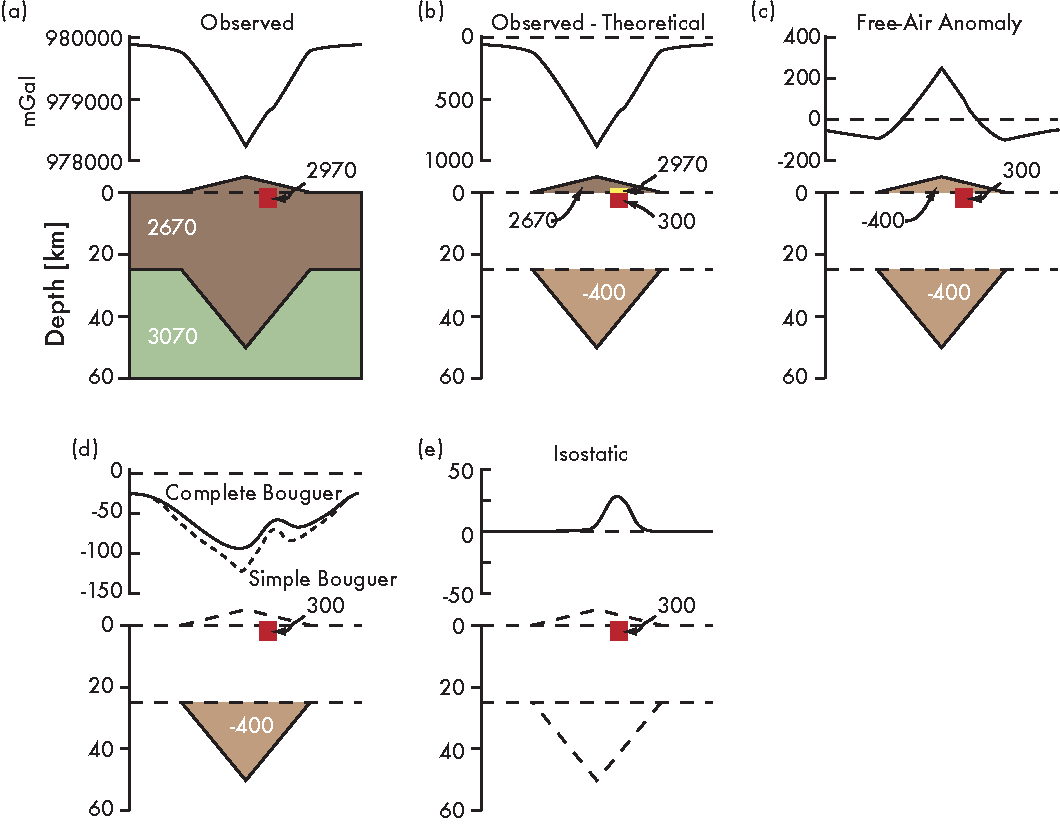
\includegraphics[width=\textwidth]{gravity/figures/gravity_corrections.pdf}
    \caption{Gravity corrections. (a) Observed gravity for a single density crust with a mountain root and an upper crustal anomaly. (b) Removing theoretical gravity (latitude correction). (c) Free-air corrected anomaly. (d) Bouguer correction (simple, slab; complete, slab + topography). (e) Isostatic corrected gravity.}
    \label{fig:gcorr}
\end{figure}

\subsubsection{Instrument Drift}
With time, properties of the gravity meter change ever so slightly resulting in slow change (drift) in readings.  This drift may be due to non-elastic stretching of the spring and mechanical dislocations in the spring at a molecular level among other things.  Essentially these are things that are difficult to impossible to account for directly.  Instrument drift can be non-linear and need not be continuous.  This makes accounting for drift somewhat challenging.  However, the standard method is to take multiple readings at a base station throughout the day (Fig.~\ref{fig:drift}).  By comparing measurements at the base throughout the day a linear-piecewise or low-order polynomial drift curve is developed which is then removed from the data by interpolation.
\begin{figure}[hbt]
    \centering
    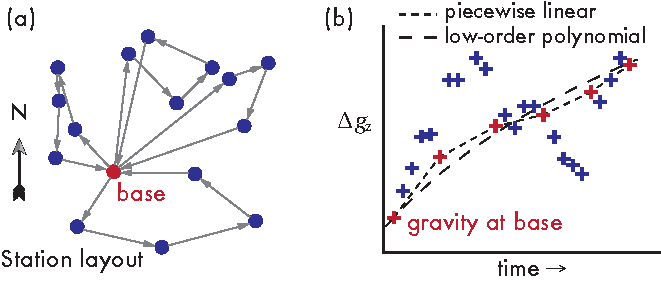
\includegraphics[]{gravity/figures/g_drift.pdf}
    \caption{An illustration of instrument drift for a collection of gravity observations made over a period of time.  (a) Site locations and observational circuits; note the multiple return trips to the base station.  (b) If there is no drift, the change in base station observations should be within observational uncertainty.  The variation throughout the day requires a drift correction, often executed with a low-order polynomial or piecewise linear function.}
    \label{fig:drift}
\end{figure}

\subsubsection{Latitude}
The rotation of Earth not only flattens its shape into a slight ellipsoid but also imparts a slight centrifugal force.  It is a bit like being pushed to the outside of a car when it makes a turn.  This centrifugal force distorts gravity field and is zero at the poles and maximum at the equator.  The latitude correction accounts for the shape and rotation of this ellipsoid and is also called the theoretical gravity.  For a derivation of the centrifugal force see
\citet{Blakely1995}.
\begin{figure}[hbt]
    \centering
    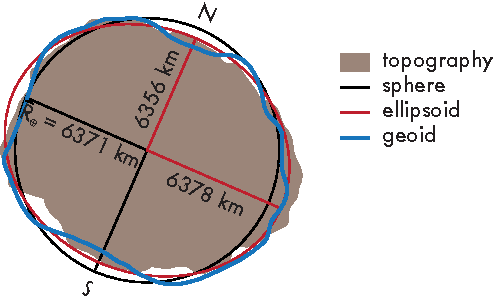
\includegraphics[]{gravity/figures/g_lat.pdf}
    \caption{The shape of Earth deviates from a sphere.  To first order, the shape is an ellipse.  The geoid is an equipotential surface of Earth.}
    \label{fig:latitude}
\end{figure}

Sometimes the latitude correction is handled by using gravity from a local absolute gravity measurement.

The theoretical gravity can be computed using the Somigliana equation,
\begin{equation}
    g_{\lambda} = g_{e} \left( 
    \frac{1 + k \sin^{2} \lambda}{(1 - e^{2} \sin^{2} \lambda)^{1/2}} \right),
\end{equation}
where $g_{e}$ is the equatorial acceleration of the spheroid, $k$ and $e$ are empirical constants.  The Geodetic Reference System 1980 included in the World Geodetic System 1984 (WGS-84), a commonly used datum, the correction is given by
\begin{equation}
    g_{\lambda} = 978032.67714
    \frac{1 + 0.00193185138639 \sin^{2} \lambda}
    {1 - 0.00669437999013^2 \sin^{2} \lambda} \mbox{ $[$mGal$]$}.
\end{equation}
(Better be using double precision numbers in computer codes!)

Sometimes this correction is handled by using observed gravity from a local absolute gravity measurement.

\subsubsection{E{\"o}tv{\"o}s}
When towing a gravity instrument behind a ship, driving in a vehicle, flying in an airplane, or orbiting in a satellite, a correction must be applied for the accelerations imparted by motion.  This correction is unnecessary for the typical land based gravity survey.

For a ship and airplane, the E{\"o}tv{\"o}s correction is given by
\begin{equation}
    g_{E} = 4.051 v \cos \lambda \sin \alpha + 0.001211 v^{2} \mbox{ $[$mGal$]$},
\end{equation}
where $v$ is the speed of travel in km~hr$^{-1}$, $\lambda$ is the latitude w.r.t.\ true north, and $\alpha$ is the heading.

\subsubsection{Tides}
The gravitational pull of the Moon and the Sun distort the shape of the solid Earth.  Hence throughout the day, the distance from a point at the surface to the gravitational center of the Earth changes.  Tides are removed by using precisely calculated tables or mathematical approximations for the location on the Earth and time of day.

\subsubsection{Free-air}
The further one is from the center of the Earth, the lower the gravitational attraction.  The free air correction accounts for the height above sea-level.  This is generally the last correction applied to marine data as there is no elevation above sea-level.

The free-air correction is given by
\begin{equation}
    g_{\mathrm{\it fa}} = 0.3086 h \mbox{ $[$mGal$]$},
\end{equation}
where $h$ is the height above the datum.

\begin{framed}
{\bf Aside:} Although this is called the free-air correction, we do not actually include the density of air, 1.2~kg~m$^{-3}$.  Is the density of air significant enough at 1000~m that we would notice an effect on gravity?

For a Bouguer slab with a density equal to air, the gravitational anomaly is
\begin{equation*}
    2 \pi (6.6725985 \times 10^{-11} \mbox{ m$^{3}$ kg$^{-1}$ s$^{-2}$})
    (1.2 \mbox{ kg m$^{-3}$}) (1000 \mbox{ m}) 
    = 5.0 \times 10^{-7} \mbox{ m s$^{-2}$},
\end{equation*}
\begin{equation*}
    5.0 \times 10^{-7} \mbox{ m s$^{-2}$} 
    \times 10^{8} \mbox{ $\mu$Gal m$^{-1}$ s$^{2}$} = 50 \mbox{ $\mu$Gal}.
\end{equation*}
This should be measurable.  Perhaps we should agree to call this the
free-vacuum calculation instead?
\end{framed}

\subsubsection{Bouguer slab}
Because the theoretical gravity and free-air correction do not incorporate the mass between the observation point and sea-level, we must apply a correction to account for this mass.  This is called the Bouguer correction and involves removing the mass for an infinite slab of height equal to the measurement location.  This resulting anomaly is called the simple Bouguer anomaly.

The Bouguer correction is given by
\begin{equation}
    g_{\mathrm{\it bs}} = 2 \pi G \rho h,
\end{equation}
where $G$ is the gravitational constant, $\rho$ is the density, and $h$ is the height above the datum.

The reduction density for the Bouguer slab correction is almost always assumed to be 2670~kg~m$^{-3}$.  Can you think of a reason this value is chosen?

Assuming the standard reduction density, the Bouguer slab correction is given by
\begin{equation}
    g_{\mathrm{\it bs}} = 0.11194 h \mbox{ $[$mGal$]$}.
\end{equation}

\subsubsection{Terrain}
Local variations in elevation surrounding the station distort the local gravity field, pulling laterally rather than vertically.  The terrain correction accounts for the additional mass above (hills/mountains) the station and missing mass below (valleys).  This correction essentially fixes our incorrect assumption of an infinite slab made in the course of a Bouguer slab correction.  While some of the corrections are simple enough that they can be done by hand---tables exist so that this one may as well---it is best performed by a computer.  This resulting anomaly is called the complex Bouguer anomaly.

\subsubsection{Isostatic}
Local topography may be affected by variations in mass at depth.  Think of mountains like icebergs, only a small percentage of the iceberg sits above the surface.  The height of an iceberg above the water is largely controlled by the amount below.  Likewise, a mountain roots affects its height.  This effect is a long wavelength feature in the gravity and by removing it, in a manner similar to the topographic correction, we can reveal gravity anomalies due to near-surface density variations. Isostasy is discussed further in Chapter~\ref{ch:isostasy}.


\section{Regional residuals}
Typically when utilizing gravity we are looking for `near' surface or `deep' structure.  Changes in observed gravity due to density variations happen over very short distances from near surface structures (short wavelengths) and happen over much longer distances from deep structure (long wavelengths); hence we can exploit this tendency to `filter' gravity.  There are a number of ways in which this residual correction is approached.  The isostatic correction, discussed in an earlier section, is one such method that attempts to reveal the near surface variations.  This section explores a additional common methods for estimating the regional or residual gravity field.  Many of these methods also work for other potential fields such as magnetics and heat flow.

While the isostatic correction has a physical foundation, the other techniques discussed below are purely mathematical meant to exploit the tendency discussed above.

\begin{framed}
\noindent {\bf Aside:} Near surface variations in density can manifest as long wavelength features.  Can you think of a situation where this might happen?  \\

\noindent Deep structures can never produce short wavelength gravity anomalies.
\end{framed}

\subsection{Visual Regression}
Visual regression is just what it sounds like.  In geophysics, we give it a very technically sounding name\ldots the `eyeball filter.'

{\bf Pros:}
\begin{itemize}
    \item Easy to implement.
    \item In a profile, this can more accurately remove regional fields than polynomial representation, although experience is often key to doing this accurately.
\end{itemize}
{\bf Cons:}
\begin{itemize}
    \item Any time you have to say ``it just looks right'' you leave yourself open to biasing the model.
    \item May not uniformly remove deep structure, or may inadvertently remove shallow structure.
    \item Computers are really fast these days and a great many methods are
    easily applied.  The eyeball filter may be good for a quick and dirty analysis in the field or boardroom, but you hate to have to justify in a paper or report that you just drew it.
\end{itemize}

\subsection{Polynomial representation}
Although there is no physical basis---it is purely mathematical---for removal of regional residuals by using low-order polynomials, it is sometimes employed because of its simplicity.  The polynomial surface is given by
\begin{equation}
    g_{\mathrm{poly}}(x,y) = \left( a_{0} + a_{1} x + a_{2} x^2 + \ldots \right)
    \left( b_{0} + b_{1} y + b_{2} y^2 + \ldots \right),
\end{equation}
where $a_{i}$'s and $b_{i}$'s are fitting constants.  The constants can be
determined using a least squares method.

{\bf Pros:}
\begin{itemize} %\setlength{\itemsep}{-5pt}
    \item Easy to implement.
    \item Easy to test higher, or lower orders.
\end{itemize}
{\bf Cons:}
\begin{itemize}
    \item You may have noticed the rather general statement `low-order'.  This is because the polynomial order is at some level up to the user's
    discretion based on the desired size/depth of target anomalies.

    \item The computed surface passes through the mean gravity and therefore the sign of the anomalies have little significance.

    \item Because the model is mathematical and not physical it may poorly fit the regional field.
\end{itemize}

\subsection{Fourier-domain filtering}
Filtering is a common operation in geophysical techniques and Fourier transforms and their inverse are an essential part of this process.  (See the supplemental notes on Fourier transforms.)  Filtering is a common way to examine only the wavelengths of interest within a signal (continuous or discrete).

By in large, the discrete Fourier transform is used most often in geophysics as we collect discretely sampled data.  A Fourier transform is performed on the data (or interpolated grid) in order to generate a set of amplitude and phases of periodic functions (sines and cosines) which describe the data.

Filtering is conducted by convolving the filter function with the gravity surface.  This is typically non-trivial in the spatial domain, but is made much simpler in the Fourier domain where it is simply a multiplication of the Fourier transform of each function.

Suppose we wish to filter the gravity map, $g(x,y)$, using a filter $f(x,y)$, then the filtered gravity $g_{f}(x,y)$ is given by
\begin{equation}
    g_f(x,y) = g(x,y) * f(x,y) \longleftrightarrow G(k_{x},k_{y}) F(k_{x},k_{y}),
\end{equation}
where $G$ and $F$ are the Fourier transforms of $g$ and $f$, respectively.  The mathematical symbol for convolution is $*$.  The spatial frequencies (wavenumbers) are expressed in terms of the spatial wavelengths $k_{x} = 2\pi \lambda_{x}^{-1}$ and $k_{y} = 2\pi \lambda_{y}^{-1}$.  To restore a gravity map, we simply apply the inverse discrete Fourier transform.  Filters are generally developed in the Fourier domain so that they have desirable properties such as removing wavelengths outside the range of interest and produce as few artifacts in the filtered result as possible.

{\bf Pros:}
\begin{itemize}
    \item Can be used to filter regional (low pass) or residual fields (high pass).
    \item Wavelengths can be specifically targeted.
    \item Fourier-domain filtering is a subject area with rich literature.  Numerous filters have been designed to reduce the addition of artifacts in the filtered field.
    \item No need to subtract off a regional field to arrive at a residual.
\end{itemize}
{\bf Cons:}
\begin{itemize}
    \item Filter design is important, a poorly designed filter can add artifacts to the data.
    \item Sparse data are subject to possible aliasing and therefore erroneous interpretation.  A serious issue with aliasing is that you will never know you have done it.
\end{itemize}

\begin{framed}
\noindent {\bf Aside:}  For a digital signal---this includes discretely sampled gravity data---the highest frequency that can be represented by within the signal is the Nyquist frequency, $f_{Ny} = (2 \Delta t)^{-1}$, where $f$ is the frequency and $t$ is time.  For spatial cases such as gravity observations this can be written, $k_{Ny} = (2 \Delta z)^{-1}$.  This really means that the absolute minimum number of times a signal must be sampled to retain the wavelength in the data is twice per cycle.  However, in practice a minimum of four times is required when noise exists (which is always).  Even at four samples per cycle there is a special case where a wavelength can be lost from the signal.  Can you think when that might occur?

When a signal is under-sampled (i.e.\ below the Nyquist frequency) we call this {\it aliasing}.  The signal is distorted from the true signal and often not in an obvious and detectable way.  To make matters worse the aliased frequencies appear as low frequencies in the data that do not really exist.

As an example, consider the Great Basin of North America where roughly north-south trending mountain ranges are separated by sedimentary basins in a near periodic way.  If one were to collect a single gravity observation within each basin, the geologic structures would be aliased within the data.  The gravity observations in this case would look like a long wavelength negative density anomaly due to the sedimentary basins.  The high density contrasting ranges would be missed from the short wavelength features and would likely appear as a very long wavelength feature.
\end{framed}

\subsection{Continuation}
\subsubsection{Gravitational potential}
Before we discuss continuation, we must first define a quantity called the gravitational potential.  At an observation point $P = (x_{0}, y_{0}, z_{0})$, with test mass $m_{0}$, the gravitational force from a mass, $m$, at point $Q = (x,y,z)$ is given by
\begin{equation}
    \vb{F} = G \frac{m m_{0}}{r^{2}}\vu{r},
\end{equation}
where and $r$ is the distance between points $P$ and $Q$, $r = \left[(x_{0} - x)^2 +
(y_{0} - y)^2 + (z_{0} - z)^2\right]^{1/2}$.  Recalling $F = m_{0} g$, the
gravitational attraction between the two points is given by
\begin{equation}
    \vb{g} = G \frac{m}{r^{2}}\vu{r} = \nabla U,
\end{equation}
where $U$ is the gravitational potential and $\nabla$ is the gradient operator.  Therefore, the potential at point $P$ is given by
\begin{equation}
    U(P) = G\int_{V} \frac{dm}{r}.
\end{equation}
Suppose the mass at $Q$ has a density distribution equal to $\rho(x_{0},y_{0},z_{0})$, then $dm = \rho(x_{0},y_{0},z_{0}) dv$.  Thus the potential can be written
\begin{equation}
    U(P) = G\int_{V} \frac{\rho(Q)}{r} dv.
    \label{eq-gpot}
\end{equation}

\subsubsection{Upward Continuation}
Although upward and downward continuation may be done from any shaped surface to any other shaped surface, it is easiest to do if we constrain ourselves from one level surface to another.  Consider a point $P = (x, y, z_{0} - \Delta z)$ such that $\Delta z$ is a positive value some distance above the surface $z_{0}$.  (Note that we define $\hat{z}$ as positive down---towards the center of the Earth.  This is a common convention in geophysics.)  It can be shown that the upward continued field is given by
\begin{equation}
    U(x,y,z_{0} - \Delta z) = \frac{\Delta z}{2 \pi} 
    \int_{-\infty}^{\infty} \int_{-\infty}^{\infty} 
    \frac{U(x',y',z_{0})} 
    {\left[(x - x')^2 + (y - y')^2 + \Delta z^2 \right]^{3/2}}
    dx' dy',
\end{equation}
where $U(x',y',z_{0})$ is given in Equation~\ref{eq-gpot}.  See \citet{Blakely1995} for a full derivation.

Upward continuation can also be expressed as a Fourier domain technique.  Let us define
\begin{equation}
    \psi_{u} = \frac{\Delta z}{2 \pi} 
    \left[(x - x')^2 + (y - y')^2 + \Delta z^2 \right]^{-3/2},
\end{equation}
which has the Fourier transform
\begin{equation}
    \mcal{F}[\psi_{u}] = e^{-|k|\Delta z}, \mbox{ z > 0}.
\end{equation}

Hence,
\begin{equation}
    \mcal{F}[U_{u}] = \mcal{F}[U]\mcal{F}[\psi_{u}],
\end{equation}
and all that needs to be done to find the upward continued field is to take the inverse Fourier transform.  The upward continued gravity, is then found by $\vb{g_{u}} = \nabla U_{u}$.

{\bf Pros:}
\begin{itemize}
    \item Relatively simple and physically based.
    \item Highlights regional variations.
    \item Allows for merging two datasets collected at different altitudes.  This is important when comparing land to airborne, airborne to airborne, airborne to satellite data. 
\end{itemize}
{\bf Cons:}
\begin{itemize}
    \item Short wavelengths are not completely removed but amplitudes are merely attenuated.  The higher the continued surface, the greater the attenuation.
\end{itemize}

\subsection{Downward Continuation}
Downward continuation is a precarious operation as it is an `un-smoothing' operation.  The downward continuation is expressed as
\begin{equation}
    \mcal{F}[U_{d}] = \mcal{F}[U]\mcal{F}^{-1}[\psi_{u}],
\end{equation}
where $\mcal{F}^{-1}[\psi_{u}]$ is $e^{+|k|z}$.  Since noise in the data are generally uncorrelated---they are short wavelength features---any noise is amplified.

{\bf Pros:}
\begin{itemize}
    \item Relatively simple.
    \item Highlights short wavelength anomalies.
\end{itemize}
{\bf Cons:}
\begin{itemize}
    \item Amplifies noise.
\end{itemize}

%\section{Image processing techniques}

\section{Densities of Earth Materials}
The density of Earth materials vary considerably from $\sim$50~kg~m$^{-3}$ for pumice to $\sim$19400~kg~m$^{-3}$ for native gold.  However, most silicates (bulk of the crust and mantle) fall between 2500 to 3400~Mg~m$^{-3}$.  A table summarizing a number of common/important materials are given in Table~\ref{tab-density}.

The density of rocks are affected by the porosity (amount of void space), and composition of the grains.  Sedimentary rocks tend to be less dense than crystalline rocks.  Igneous rock densities are largely controlled by their silica content (SiO$_{2}$).  The more SiO$_{2}$ the less dense the rock.  Most ores are very dense making gravity a good exploration tool.

Bulk can be predicted from the densities of their individual components using a mixing relationship.  A mixing relationship is essentially an average of which a great number have been devised.  For density a rock with several mineral constituents each with a density $\rho_{i}$ and volume fraction $v_{i}$.  Within a given volume, the mass of each component is $v_{i} \rho_{i}$, then dividing by the total volume then will give us the effective (or bulk) density,
\begin{equation}
    \rho_{bulk} = \frac{\sum_{i=1}^{N} v_{i} \rho_{i}}{\sum_{i=1}^{N} v_{i}}.
\end{equation}
Hence the effective density is just the arithmetic mean of the components.  Note that this works as well when rocks have pore space.  In such a case, the pore space must be included as a constituent, (i.e.,\ $\phi \rho_{\phi}$, where $\phi$ is the porosity and $\rho_{phi}$ is the density of the air, oil, gas, or water, filling the pore space).
\begin{table}
    \begin{threeparttable}
    \caption{Table of rock and mineral densities in \si{kg.m^{-3}}.}
    \label{tab-density}
    \begin{tabular}{@{}lclclc@{}}
        \toprule
        Rock Type &
        Density Range &
        Material Type &
        Density Range & 
        Material Type &
        Density Range \\

        \midrule
        \multicolumn{2}{c}{\it Sediments (wet)} & \multicolumn{2}{c}{\it Oxides} & \multicolumn{2}{c}{\it Sulfates} \\
        soil        & 1200--2400    & hematite      & 4900--5300 & gypsum        & 2200--2600 \\
        clay        & 1630--2600    & magnetite     & 4900--5200 & barite        & 4300--4700 \\
        gravel      & 1700--2400    & ilmenite      & 4300--5000 \\
        sand        & 1700--2300    & rutile        & 4180--4300 & \multicolumn{2}{c}{\it Native Elements} \\
        sandstone   & 1610--2670    & chromite      & 4200--4600 & copper        & 8700 \\
        shale       & 1770--3200    & cuprite       & 5700--6150 & silver        & 10500 \\
        limestone   & 1930--2900    & manganite     & 4200--4400 & gold          & 15600--19400 \\
        dolomite    & 2280--2900    & cassiterite   & 6800--7100 & coal          & 1200--1800 \\
        {}          & {}            & wolframite    & 7100--7500 & graphite      & 1900--2300 \\
        \multicolumn{2}{c}{\it Igneous Rocks} & uraninite     & 8000--9970 \\
        tuff        & 1000--2400    & {}            & {}         & \multicolumn{2}{c}{\it Non-metallic} \\
        rhyolite    & 2350--2700    & \multicolumn{2}{c}{\it Hydroxides} & salt          & 210--2600 \\
        granite     & 2500--2810    & bauxite       & 2300--2550 & ice           & 880--920 \\
        granodiorite & 2670--2790   & {}            & {}         & sea water     & 1010--1050 \\
        andesite    & 2400--2800    & \multicolumn{2}{c}{\it Carbonates} & fluorite      & 3010--3250 \\ 
        diorite     & 2720--2990    & calcite       & 2710 \\
        basalt      & 2700--3300    & aragonite     & 2950 \\
        diabase     & 2500--3200    & dolomite      & 2280--2900 \\
        gabbro      & 2700--3500    & siderite      & 3700--3900 \\
        peridotite  & 3200--3370    & magnesite     & 2900--3120 \\
        pyroxenite  & 3200--3370    \\
        {}          & {}            & \multicolumn{2}{c}{\it Sulfides} \\
        \multicolumn{2}{c}{\it Metamorphic Rocks} & pyrite        & 4900--5200 \\
        graywacke   & 2600--2700    & pyrrhotite    & 4500--4800 \\
        slate       & 2700--2900    & sphalerite    & 3500--4000 \\
        quartzite   & 2500--2700    & chalcopyrite  & 4100--4300 \\
        marble      & 2600--2900    & covellite     & 4600--4800 \\
        schist      & 2390--2900    & chalcocite    & 5500--5800 \\
        amphibolite & 2900--3040    & malachite     & 3900--4030 \\
        gneiss      & 2590--3000    & molybdenite   & 4400--4800 \\
        eclogite    & 3200--3540    & cobaltite     & 5800--6300 \\
        serpentine  & 2400--3100    & stannite      & 4300--4520 \\
        {}          & {}            & galena        & 7400--7600 \\
        {}          & {}            & cinnabar      & 8000--8200 \\
        \bottomrule
    \end{tabular}
    \begin{tablenotes}
        \item After \citet{Telford_etal1990} pg. 16.
    \end{tablenotes}
    \end{threeparttable}
\end{table}

\nocite{Blakely1995}
\nocite{Chapin1998}
\nocite{Grant&West1965}
\nocite{Lowrie1997}
\nocite{Reynolds1997}
\nocite{Telford_etal1990}

\bibliographystyle{elsarticle-harv}
\bibliography{ref}

\chapter[Isostasy]{Isostasy\\ \large Gravity Extension}\label{ch:isostasy}

\section*{Introduction}

Isostasy refers to an equilibrium state of buoyancy, much like an iceberg floating in the ocean.  Approximately 10\% of an iceberg rises above the water surface, with the remaining 90\% hidden from view.  For icebergs of different size, larger ice masses extend both higher above and deeper below the waterline.  Placing a series of icebergs side by side would produce relief above the surface and compensating roots below, a configuration that closely parallels topography and its subsurface support within the Earth.

\emph{Isostasy} describes a state of mechanical equilibrium in which \emph{lateral variations} in mass (loads) are arranged such that pressure is balanced at a common depth, known as the \emph{depth of compensation}.  Isostasy is an equilibrium condition, not a physical process.  The mechanisms by which the Earth approaches or departs from this state—such as elastic flexure, viscous mantle flow, erosion, sedimentation, and thermal contraction—are referred to as \emph{isostatic processes}.  Throughout this chapter, we will distinguish carefully between isostasy as a state and isostatic processes as the means by which that state is modified or restored.

Because isostatic balance depends on vertically integrated mass, it carries no intrinsic vertical resolution.  Different distributions of density and thickness can satisfy the same isostatic condition.  Moreover, the presence of lithospheric strength means that isostatic equilibrium is commonly approached rather than achieved, and often only over long spatial and temporal scales.

In this chapter we develop the concept of isostasy as a constraint on mass distribution, examine idealized end-member formulations, and explore how departures from equilibrium provide insight into lithospheric strength, mantle rheology, and thermal evolution.

\section{Isostasy Theory}
The pressure-balance condition developed in this section should be understood as one limit of a more general problem: how a lithosphere of finite mechanical strength supports surface loads. When lithospheric strength is negligible, that general problem reduces to the local, column-by-column balance developed below. When lithospheric strength is significant---\emph{almost always}, loads are instead partially or wholly supported by flexure rather than buoyancy alone, a case we return to later in this chapter once the strength-free limit has been fully developed.
\begin{itemize}
  \item Definition of isostatic equilibrium as lateral pressure balance at a reference depth.
  \item Emphasis on column-integrated mass (or density--thickness products) rather than detailed vertical structure.
\end{itemize}

The mechanical expression of isostatic equilibrium is a balance of pressure at a common depth at which neighboring lithospheric columns exert equal normal stress.  This balance is evaluated using vertically integrated properties of the columns, so isostasy constrains density--thickness products rather than detailed vertical structure.

The physical basis for this balance is buoyancy, which requires a fluid substratum to balance pressure at depth. While the mantle responds elastically and behaves as a solid at short timescales, at geologic time scales, the upper mantle beneath the lithosphere behaves as a very high-viscosity fluid---a \emph{geophysical fluid}.  This fluid-like behavior allows lateral pressure gradients to relax.  Isostasy therefore describes the long-term equilibrium state that emerges only because the mantle is capable of slow, viscous flow.

\textbox{Mantle: Solid or Liquid?}{

The Earth's mantle is solid and crystalline, even though we frequently describe its behavior using fluid-related concepts.  We speak of mantle buoyancy, melt generation, viscosity, flow-induced seismic anisotropy, and convection, all of which are ideas drawn from fluid mechanics.  Aside from partial melt---typically no more than $2$--$3$\% and largely confined to the asthenosphere before percolating into the lithosphere---the mantle is solid rock.  This solid nature is demonstrated most directly by the efficient transmission of seismic shear waves, which cannot propagate through liquids.

Over long time scales and at high temperatures, however, the mantle can deform by viscous creep.  This deformation produces flow-related seismic anisotropy through the preferential alignment of olivine crystals, while lateral temperature gradients generate buoyancy forces that drive mantle convection.  Isostasy relies on this long-term viscous behavior, not on the presence of melt, to restore isostatic equilibrium.  The mantle's viscosity resists deformation, which is why these fluid-like processes typically occur at rates of millimeters to tens of millimeters per year.  Consequently, the time scales over which isostatic and convective adjustments occur range from thousands to millions of years.

For this reason, the mantle is often described as a \emph{geophysical fluid}: a solid that behaves like a fluid only when observed over sufficiently long spatial and temporal scales.
}{aside}
% A useful historical analogy comes from Archimedes' principle.  According to the well-known (and likely apocryphal) story, Archimedes was tasked by King Hiero~II with determining whether a crown was made of pure gold without destroying it.  The solution relied on the observation that an object immersed in a fluid experiences an upward buoyant force equal to the weight of the displaced fluid.  Whether or not the story is true, Archimedes' principle provides the physical basis for our understanding of buoyancy and floating equilibrium.

% In the Earth, the lithosphere overlies a mechanically weak region of the upper mantle known as the asthenosphere.  Over sufficiently long time scales, the asthenosphere behaves as a fluid, allowing the overlying lithosphere to establish an equilibrium elevation determined by its buoyancy.  This equilibrium condition is referred to as \emph{isostatic equilibrium}.  Variations in surface elevation may therefore be interpreted as arising from lateral variations in the buoyancy of lithospheric columns.

\subsection{Column balance and isostatic equilibrium}

Consider a vertical column of lithosphere exerting a force on the underlying asthenosphere.
Although isostatic equilibrium can be expressed as a balance of forces, it is more convenient to work with pressure (force per unit area), which follows directly by writing the weight of a column,
\begin{equation}
    \frac{F}{A} = \frac{m g}{A} = \rho h g .
\end{equation}
This formulation allows neighboring lithospheric columns to be compared independent of their horizontal extent.
\begin{figure}[hbt]
    \centering
    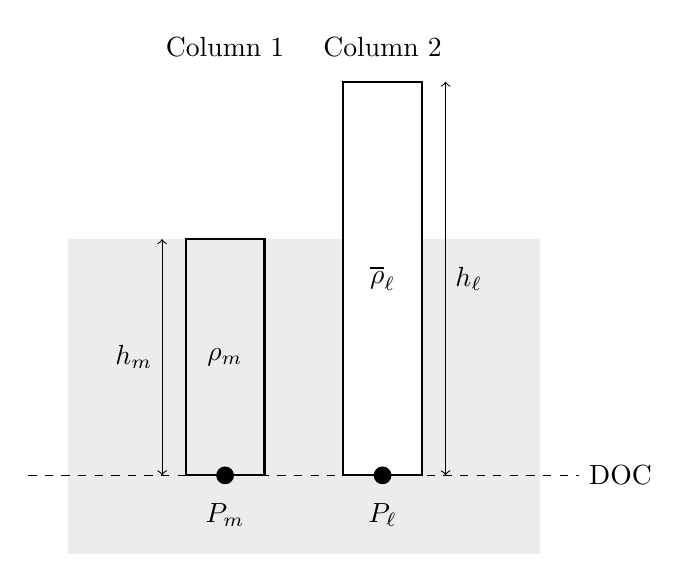
\begin{tikzpicture}[scale=1.0]

        % Asthenosphere
        \fill[gray!15] (-1.5,-1) rectangle (4.5,3);

        % Elevation difference
        \draw[<->] (-0.3,0) -- (-0.3,3) node[midway,left] {$h_m$};

        \draw[thick] (0,0) rectangle (1,3);
        \node[above] at (0.5,5.2) {Column 1};
        \draw[fill=black] (0.5,0) circle (3pt);
        \node at (0.5,1.5) {$\rho_m$};
        \node at (0.5,-0.5) {$P_m$};

        % Columns 1
        \draw[thick,fill=white] (2,0) rectangle (3,5);
        \node[above] at (2.5,5.2) {Column 2};
        \draw[fill=black] (2.5,0) circle (3pt);
        \node at (2.5,-0.5) {$P_\ell$};

        % Heights
        \draw[<->] (3.3,0) -- (3.3,5) node[midway,right] {$h_{\ell}$};

        % Compensation depth
        \draw[dashed] (-2,0) -- (5.0,0) node[right] {DOC};

        % Labels
        \node at (2.5,2.5) {$\overline{\rho}_{\ell}$};

    \end{tikzpicture}
    \caption{Schematic columns for the mantle and a column of lithosphere buoyantly supported at isostatic equilibrium. Pressure is balanced at a depth of compensation (DOC).}
    \label{fig:columns1}
\end{figure}

Isostatic equilibrium is therefore expressed as a balance of pressure at a common depth of equal normal stress.  Consider a vertical column of lithosphere of height $h_{\ell}$ and average density $\overline{\rho}_{\ell}$ overlying asthenospheric material of density $\rho_m$ (Figure~\ref{fig:columns1}).  The downward pressure exerted by the lithospheric column is
\[
    P_{\ell} = \overline{\rho}_{\ell} h_{\ell} g .
\]
For the column to be in isostatic equilibrium, this pressure must be balanced by the pressure of displaced asthenospheric material,
\[
    P_m = \rho_m h_m g ,
\]
where $h_m$ is the height of the displaced fluid column.  The net vertical pressure is given by
\[
    P_{\mathrm{net}} = 0 = \overline{\rho}_{\ell} h_{\ell} g - \rho_m h_m g .
\]

Importantly, this expression shows that isostasy depends on vertically integrated quantities.  Only the product of density \emph{and} thickness enters the balance; detailed vertical variations in density within the column are not resolved.  In this sense, isostasy provides no intrinsic vertical resolution.

\subsection{Lateral pressure balance and the depth of compensation}

Isostasy is fundamentally a lateral constraint.  Consider two neighboring lithospheric columns with different buoyancies and elevations (Figure~\ref{fig:columns2}).  For each column, the pressure balance may be written as
\begin{align*}
    \text{Column 1:} \quad 
    P_{\mathrm{net},1} &= \overline{\rho}_{\ell,1} h_{\ell,1} g - \rho_m h_{m,1} g , \\
    \text{Column 2:} \quad
    P_{\mathrm{net},2} &= \overline{\rho}_{\ell,2} h_{\ell,2} g - \rho_m h_{m,2} g .
\end{align*}
\begin{figure}[hbt]
    \centering
    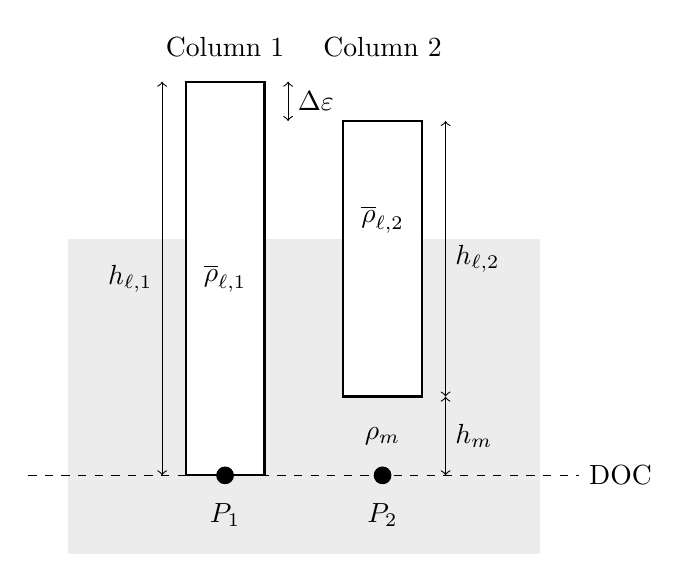
\begin{tikzpicture}[scale=1.0]

        % Asthenosphere
        \fill[gray!15] (-1.5,-1) rectangle (4.5,3);

        % Columns 1
        \draw[thick,fill=white] (0,0) rectangle (1,5);
        \node[above] at (0.5,5.2) {Column 1};
        \draw[fill=black] (0.5,0) circle (3pt);
        \node at (0.5,-0.5) {$P_1$};

        % Columns 2
        \draw[thick,fill=white] (2,1) rectangle (3,4.5);
        \node[above] at (2.5,5.2) {Column 2};
        \draw[fill=black] (2.5,0) circle (3pt);
        \node at (2.5,-0.5) {$P_2$};

        % Heights
        \draw[<->] (-0.3,0) -- (-0.3,5) node[midway,left] {$h_{\ell,1}$};
        \draw[<->] (3.3,0) -- (3.3,1) node[midway,right] {$h_m$};
        \draw[<->] (3.3,1) -- (3.3,4.5) node[midway,right] {$h_{\ell,2}$};
        \draw[<->] (1.3,4.5) -- (1.3,5) node[midway,right] {$\Delta\varepsilon$};

        % Compensation depth
        \draw[dashed] (-2,0) -- (5,0) node[right] {DOC};

        % Labels
        \node at (0.5,2.5) {$\overline{\rho}_{\ell,1}$};
        \node at (2.5,3.25) {$\overline{\rho}_{\ell,2}$};
        \node at (2.5,0.5) {$\rho_m$};

    \end{tikzpicture}
    \caption{Schematic lithospheric columns in isostatic equilibrium. Pressure is balanced at a common depth (DOC), while surface elevations differ due to variations in integrated buoyancy of each column.}
    \label{fig:columns2}
\end{figure}

If both columns are in isostatic equilibrium, their net pressures must be equal,
\begin{align*}
    P_{\mathrm{net},1} &= P_{\mathrm{net},2} , \\
    \overline{\rho}_{\ell,1} h_{\ell,1} g - \rho_m h_{m,1} g 
    &= \overline{\rho}_{\ell,2} h_{\ell,2} g - \rho_m h_{m,2} g .
\end{align*}

Rearranging gives
\begin{equation}
    \overline{\rho}_{\ell,1} h_{\ell,1} g
    =
    \overline{\rho}_{\ell,2} h_{\ell,2} g + \rho_m h_m g ,
    \label{eq:isostatic_pressure}
\end{equation}
where $h_m = h_{m,1} - h_{m,2}$.
Equation~\ref{eq:isostatic_pressure} expresses the requirement that pressures be equal at a common reference depth.
This depth is known as the \emph{depth (or level) of compensation} (Figure~\ref{fig:isostasy2}).

The equilibrium elevation difference between the two columns,
$\Delta \varepsilon = \varepsilon_1 - \varepsilon_2$,
may be written as
\begin{equation}
    \Delta \varepsilon = h_{\ell,1} - (h_{\ell,2} + h_m) .
    \label{eq:isostatic_elevation}
\end{equation}

Together, Eqs.~\ref{eq:isostatic_pressure} and \ref{eq:isostatic_elevation} show that differences in elevation arise from differences in column-integrated buoyancy.
Both density and thickness variations may contribute, and in general neither can be uniquely determined without additional assumptions.



\subsection{Interpretation and limitations}

In practice, lithospheric columns often consist of multiple layers.
In such cases the average density is an arithmetic weighted mean,
\begin{align*}
    \overline{\rho} &= \frac{1}{h} \sum_{i=1}^{N} \rho_i h_i , \\
    h &= \sum_{i=1}^{N} h_i .
\end{align*}

Isostatic analysis rests on several implicit assumptions:
\begin{itemize}
    \item Vertical forces other than buoyancy are negligible.
    Dynamic mantle flow may exert additional vertical stresses, producing elevation anomalies that are not isostatic in origin.
    \item The lithosphere offers no lateral resistance to deformation.
    In reality, lithospheric strength allows loads to be regionally supported by flexure; local isostasy is therefore best regarded as an end-member approximation.
    \item The system is in equilibrium.
    When density or thickness changes occur rapidly (e.g., glacial unloading, erosion, delamination), the lithosphere requires time to adjust toward a new isostatic state.
\end{itemize}

These limitations emphasize that isostasy is a constraint on admissible mass distributions, not a complete physical description of lithospheric deformation.
Gravity anomalies reflect both isostatic structure and departures from equilibrium, and isostasy therefore reduces—but does not eliminate—the non-uniqueness inherent in gravity interpretation.

\subsection{Local isostatic end-members}

\subsubsection{End-member nature of idealized models}

The simplest formulations of isostasy are local models, in which each lithospheric column is assumed to be independently supported by buoyancy forces.  Two classical end-member formulations, commonly known as Airy and Pratt isostasy, are widely used to illustrate how lateral variations in elevation may arise.

These models should be understood as \emph{limiting cases}, not as competing or mutually exclusive mechanisms.  Airy-type behavior isolates the effects of thickness variation at fixed density, whereas Pratt-type behavior isolates the effects of lateral density variation with a common base.  In the Earth, isostatic balance generally involves simultaneous variations in both density and thickness, and real solutions may be expressed as combinations of these end-members.

As a result, it is generally inappropriate to assign specific tectonic environments uniquely to one isostatic model.  The value of these end-members lies in their interpretive clarity rather than in their literal applicability.  Both end-members, and the general balance from which they derive, share the same underlying assumption of \emph{zero} lithospheric strength; Section~\ref{sec:regional_compensation} revisits this assumption directly.

\ntextbox{A brief history of local isostatic models}{

The two classical end-member models of local isostasy were published in the same year, 1855, but arose from very different motivations.  Archdeacon John Pratt developed his formulation while analyzing gravity observations collected across the Himalaya.  At that time, they didn't have gravimeters.  The direction of local vertical gravity was made by using a plumb line (a mass on the end of a spring) referenced to the stars for precise orientatation.  Pratt's measurements revealed an apparent mass deficiency beneath regions of high elevation, leading Pratt to propose that mountain ranges are underlain by lower density material rather than by thickened crust \citep{Pratt1855}.  In his interpretation, the base of the crust is flat, and surface topography reflects lateral variations in average density resulting from varying composition of the crust.

Later in the same year, Sir George Airy proposed an alternative explanation after reading Pratt's work \citep{Airy1855}.  Airy was the Astronomer Royal based at the Greenwich Royal Observatory at the time.  His office overlooked the Thames River.  In the spring, loggers would float felled trees down the river to the sawmills, providing inspiration for Airy's alternative model.  As an analogy for Earth's crust, Airy noted that all logs have similar density, those with larger diameters extend both higher above and deeper below the water surface.  This lead Airy to assume instead that crustal density is uniform and that surface relief is supported by variations in crustal thickness, with mountains underlain by buoyant roots extending into the mantle.

Although these formulations are often presented as competing models, neither is intended to describe all geological situations.  Rather, Pratt-type and Airy-type behavior represent limiting cases that isolate the roles of density and thickness variations, respectively.
Modern interpretations of isostasy generally involve combinations of both effects---lateral variations in both lithospheric density and thickness.
}{aside}

\subsubsection{Airy-type behavior}

In the Airy end-member, lithospheric density is assumed to be laterally uniform, while thickness varies.  Differences in surface elevation are accommodated by variations in the thickness of the crust, commonly conceptualized as buoyant roots extending into the underlying mantle.

Consider two crustal columns of equal density $\rho_c$, with one column thicker than the other (Figure~\ref{fig:isostasy}).  Let the thicker column extend to a deeper level through a compensating root beneath the region of higher elevation.  In this case, the difference in elevation $\Delta \varepsilon$ between the two columns may be written as
\[
    \Delta \varepsilon = (h_2 - h_1)\left(1 - \frac{\rho_c}{\rho_m}\right),
\]
where $\rho_m$ is the density of the underlying mantle.
\begin{figure}[hbt]
  \centering
  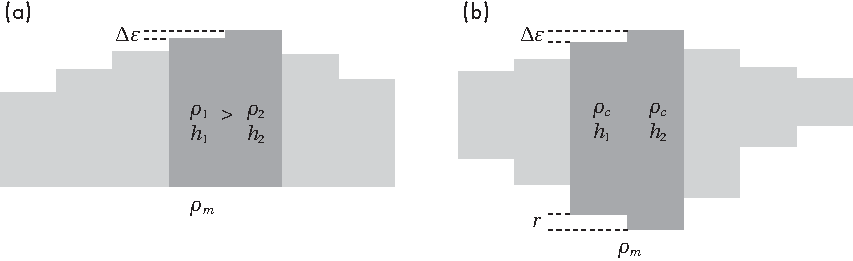
\includegraphics[]{gravity/figures/isostasy.pdf}
  \caption{Schematic comparison of (a) Pratt-type and (b) Airy-type local isostatic end-members. Both represent limiting cases of isostatic balance.}
  \label{fig:isostasy}
\end{figure}

Airy-type behavior is commonly invoked when interpreting crustal roots beneath mountain belts and plateaus.  However, isostatic balance alone does not uniquely constrain the geometry or depth extent of such roots.  Additional information from seismology or other geophysical observations is required to resolve vertical structure.

\subsubsection{Pratt-type behavior}

In the Pratt end-member, lithospheric thickness is assumed to be laterally uniform, while density varies from column to column.
Differences in elevation arise from lateral variations in mass per unit volume rather than from variations in thickness.

Historically, Pratt developed this formulation based on gravity observations across the Himalaya, which suggested a mass deficiency beneath regions of high elevation \citep{Pratt1855}.
In this interpretation, the base of the crust is flat, and topographic relief reflects decreasing average density toward the interior of the mountain range (Figure~\ref{fig:isostasy}a).
Airy later proposed the complementary thickness-variation model after reading Pratt's work \citep{Airy1855} (Figure~\ref{fig:isostasy}b).

For two crustal columns of equal thickness but different densities $\rho_1$ and $\rho_2$, the resulting elevation difference may be expressed as
\[
    \Delta \varepsilon = h \left(\frac{\rho_1}{\rho_2} - 1\right),
\]
where $h$ is the common column thickness.

Pratt-type behavior highlights the role of density variations arising from compositional differences or temperature variations.  For this reason, it provides a natural conceptual bridge to thermal isostasy, which is developed later in the chapter and revisited in the context of lithospheric cooling models (Chapter~\ref{ch:geothermics2}).

\section{Thermal Isostasy}\label{sec:thermal_isostasy}

Before connecting isostasy to gravity and flexure, it is useful to isolate the role of temperature.  Thermal isostasy arises from lateral variations in temperature that modify density and therefore buoyant support. In many tectonic settings, observed elevation differences cannot be explained solely by variations in crustal thickness or composition, but instead reflect differences in the thermal structure of the lithosphere and upper mantle.

A common strategy is to normalize each lithospheric column to a reference or \emph{standard column} defined by an average crustal thickness and average composition. Compositional and thickness effects are accounted for first, and any remaining elevation difference is then attributed to thermal buoyancy. In this framework, the total isostatic elevation difference may be written as
\begin{equation}
    \Delta \varepsilon_{\mathrm{total}}
    =
    \Delta \varepsilon_{\mathrm{compositional}}
    +
    \Delta \varepsilon_{\mathrm{thermal}} .
\end{equation}
This decomposition assumes local isostatic compensation and neglects flexure and dynamic pressure gradients in the mantle.

\subsection{Normalization to a standard column}

Consider a lithospheric column composed of \(N\) layers of thickness \(h_i\) and density \(\rho_i\), overlying a mantle of density \(\rho_m\). Let the reference column have corresponding quantities \(h_i^{\mathrm{ref}}\) and \(\rho_i^{\mathrm{ref}}\), chosen to represent average crustal structure.

Under local isostatic equilibrium, pressure balance at the depth of compensation requires that the vertically integrated mass of the column equal that of the reference column minus any elevation difference. The compositional and thickness contribution to elevation relative to the reference column is therefore
\begin{equation}
    \Delta \varepsilon_{\mathrm{compositional}}
    =
    \frac{1}{\rho_m}
    \sum_{i=1}^{N}
    \left(
        \rho_i h_i
        -
        \rho_i^{\mathrm{ref}} h_i^{\mathrm{ref}}
    \right).
\end{equation}

This expression corrects the observed elevation for differences in crustal thickness and composition relative to the standard column. Once this correction is applied, the remaining elevation signal is attributed to thermal effects.

\subsection{Thermal buoyancy and density variation}

Thermal isostasy follows from the temperature dependence of density. For small departures from a reference geotherm, density may be approximated as
\[
\rho(T) \approx \rho_0 \left[1 - \alpha \left(T - T_{\mathrm{ref}}\right)\right],
\]
where \(\alpha\) is the coefficient of thermal expansion, \(T(z)\) is the geotherm of interest, and \(T_{\mathrm{ref}}(z)\) is a reference geotherm.

Because isostasy depends on vertically integrated mass, the thermal contribution to elevation is obtained by integrating the temperature difference between the two columns,
\begin{equation}
    \Delta \varepsilon_{\mathrm{thermal}}
    =
    \alpha
    \int_{0}^{z_{\mathrm{max}}}
    \left[ T(z) - T_{\mathrm{ref}}(z) \right] \, dz,
\end{equation}
where \(z_{\mathrm{max}}\) is the depth over which thermal density differences contribute significantly to buoyancy.

\subsection{Piecewise geotherms}

In practice, geotherms are often represented as piecewise functions within depth intervals. In this case, the elevation contribution from the \(i\)-th depth interval is
\begin{equation}
    \varepsilon_i
    =
    \alpha
    \int_{z_i}^{z_{i+1}}
    \left[ T(z) - T_{\mathrm{ref}}(z) \right] \, dz,
\end{equation}
and the total thermal elevation is obtained by summing over all intervals,
\begin{equation}
    \Delta \varepsilon_{\mathrm{thermal}}
    =
    \sum_{i=1}^{N} \varepsilon_i .
\end{equation}

Because the integral operator is linear, each term may be evaluated by integrating the geotherms separately and taking the difference,
\begin{equation}
    \varepsilon_i
    =
    \alpha
    \left[
        \int_{z_i}^{z_{i+1}} T(z)\, dz
        -
        \int_{z_i}^{z_{i+1}} T_{\mathrm{ref}}(z)\, dz
    \right].
\end{equation}
This formulation makes no assumptions about the functional form of the geotherms.

Thermal isostasy provides a direct link between geothermics and surface observables. Cooling of the lithosphere increases density and produces subsidence, while elevated temperatures reduce density and produce buoyant uplift. These effects account for much of the long-wavelength elevation signal observed over oceanic plates, continental interiors, and magmatic provinces.

In later chapters, we return to thermal isostasy in the context of half-space and plate cooling models, where explicit geotherms are developed and time-dependent subsidence and uplift can be calculated. In those settings, thermal isostasy provides the physical connection between thermal evolution, surface topography, and long-wavelength gravity anomalies.


\section{Relationship between Gravity and Isostasy}

Gravity and isostasy are closely related but fundamentally distinct concepts.  Gravity describes the acceleration field produced by a distribution of mass, whereas isostasy describes a mechanical equilibrium state of that mass distribution.  As a result, gravity observations may reflect both isostatic equilibrium and departures from it, but gravity alone does not determine whether isostatic balance has been achieved.

In an isostatically compensated system, lateral variations in surface elevation are supported by corresponding variations in mass at depth.  These compensating masses reduce the long-wavelength gravity signal that would otherwise be produced by topography alone.  Conversely, gravity anomalies often arise from departures from perfect isostatic balance, whether due to incomplete compensation, lithospheric strength, or time-dependent adjustment.  In this sense, gravity anomalies provide information about isostatic state, not isostasy itself.

Isostasy therefore acts as a physically motivated constraint on gravity interpretation.  By restricting the class of admissible lateral mass distributions, isostatic assumptions reduce the non-uniqueness inherent in gravity analysis, but they do not eliminate it.  Different combinations of density and thickness variations can satisfy the same isostatic condition while producing similar gravity fields.

The connection between gravity and isostasy is most clearly seen by considering vertical force balance expressed as a pressure balance at a common depth of equal normal stress.  When written in terms of pressure, each contributing term is proportional to the product $\rho h g$.  Because the gravitational acceleration $g$ multiplies all terms equally, it cancels when pressures are equated between neighboring columns.  Isostatic equilibrium therefore does not depend on the magnitude of the gravity field, but on relative variations in vertically integrated mass.

This cancellation highlights an important conceptual point.  Isostasy is not a statement about the gravity field itself, but about buoyant support provided by the underlying mantle.  Gravity governs the weight of a column, but isostasy describes how that weight is balanced by the displacement of material at depth.  The absence of an explicit gravity term in the final equilibrium condition does not imply that gravity is irrelevant; rather, gravity has already been accounted for in establishing vertical force balance.

Because isostatic balance depends only on column-integrated quantities, it provides no direct information on how mass is distributed with depth within a column.  A shallow low-density anomaly and a deeper high-density anomaly may contribute equally to the pressure balance while producing very different gravity signatures.  This limitation underscores the complementary roles of gravity and isostasy: gravity is sensitive to the spatial distribution of mass, whereas isostasy constrains only the integrated effect required for mechanical equilibrium.

\subsection{Isostatic residual gravity}\label{sec:isostatic_residual}

Isostatic corrections are commonly applied to gravity data to suppress long-wavelength gravity variations associated with the isostatic support of topography. One widely used and operationally simple formulation is that of \citet{Simpson_etal1986}, who constructed an isostatic residual gravity map of the conterminous United States to emphasize gravity anomalies arising from lateral density variations within the crust.

\subsection{Conceptual basis}

The method of \citet{Simpson_etal1986} assumes local Airy--Heiskanen isostatic compensation. In this formulation, surface topography is supported by a crustal root of variable thickness and constant density contrast with the mantle. Because Bouguer and terrain corrections already remove the gravitational attraction of surface topography, the isostatic correction is applied to the Bouguer gravity anomaly and accounts only for the gravitational effect of the subsurface compensating mass.

The isostatic residual gravity anomaly is defined as
\[
    \Delta g_{\mathrm{iso\text{-}res}}(x,y) =
    \Delta g_{\mathrm{B}}(x,y) - \Delta g_{\mathrm{root}}(x,y),
\]
where $\Delta g_{\mathrm{B}}$ is the complete Bouguer anomaly and $\Delta g_{\mathrm{root}}$ is the gravity effect of the compensating crustal root.

Under local Airy isostasy, pressure balance at a common depth of compensation requires that the surface load be balanced by a buoyant root such that
\[
    \rho_c h(x,y) + \left( \rho_m - \rho_c \right) r(x,y) = 0,
\]
where $h(x,y)$ is the surface elevation relative to sea level, $\rho_c$ is the average crustal density, $\rho_m$ is the mantle density, and $r(x,y)$ is the thickness of the compensating root.

Solving for the root thickness yields
\[
    r(x,y)
    =
    \frac{\rho_c}{\rho_m - \rho_c}\, h(x,y).
\]
This relation allows the geometry of the compensating root to be determined directly from gridded topographic and bathymetric data.

The compensating root is treated as a subsurface density anomaly relative to the surrounding mantle with density contrast
\[
    \Delta \rho = \rho_c - \rho_m .
\]
For continental crust overlying denser mantle, this contrast is negative, and the root represents a mass deficit. The root extends downward from the Moho to the depth of compensation beneath regions of positive topography, and upward beneath regions of negative relief if bathymetry is included.

The gravity effect of the compensating root is computed using standard forward-gravity methods. In continuous form, the vertical component of the gravitational acceleration produced by the root at the observation point $\vb{r}$ is given by
\[
    \Delta g_{\mathrm{root}}(\vb{r}) =
    G \iiint
    \frac{\Delta \rho(\vb{r'}) \, (z - z')} {|\vb{r} - \vb{r'}|^3}
    \, \dd{V'} ,
\]
where the integral is taken over the volume occupied by the compensating root.

In practice, the root is discretized as a set of laterally varying vertical columns derived from gridded topography. The gravity effect is evaluated numerically and subtracted from the Bouguer anomaly to yield the isostatic residual gravity field \citep{Simpson_etal1986}.

\subsection{Interpretation of isostatic residual anomalies}

Isostatic residual gravity anomalies primarily reflect lateral density variations within the crust rather than the degree of isostatic compensation. Importantly, large residual anomalies can be produced by crustal heterogeneity even when the lithosphere is in complete local isostatic equilibrium.

Consequently, isostatic residual gravity maps are best interpreted as emphasizing the gravity signature of:
\begin{itemize}
    \item lateral density contrasts in the upper and middle crust,
    \item sedimentary basins and volcanic provinces,
    \item intrusive bodies and basement structure,
    \item regional tectonic fabrics.
\end{itemize}

\citet{Simpson_etal1986} emphasize that isostatic residual anomalies should not be interpreted as indicators of isostatic disequilibrium. Instead, the primary value of the correction is the suppression of long-wavelength gravity contributions associated with crustal thickness variations required to support topography.

\subsection{Relation to spectral filtering}

Although formulated in the spatial domain, the Simpson et~al.~(1986) isostatic correction effectively acts as a physically motivated long-wavelength gravity filter. Because isostatically compensated topography contributes mainly to long wavelengths, removing the gravity effect of the compensating root attenuates these wavelengths without imposing an arbitrary spectral cutoff.

This behavior explains why isostatic residual gravity maps often resemble high-pass filtered gravity fields, while retaining a clear physical interpretation tied to crustal buoyancy rather than purely mathematical filtering.

\subsection*{Summary}

Isostatic residual gravity anomalies are constructed by removing the gravity effect of an assumed compensating mass from the Bouguer gravity field. The method of \citet{Simpson_etal1986} provides a practical and widely adopted framework for isolating gravity signals associated with shallow crustal density variations, while explicitly acknowledging the interpretive limitations imposed by isostatic assumptions.

\section{Regional compensation and lithospheric strength}\label{sec:regional_compensation}

\subsection{Breakdown of local isostasy}
Local isostatic formulations assume that each lithospheric column responds independently to loading and unloading. Essentially, local isostasy assumes that the lithosphere holds no inherent strength. This assumption is reasonable at long wavelengths and over sufficiently long time scales, but it breaks down when loads vary over short horizontal distances or when the lithosphere possesses significant mechanical strength. In such cases, topographic and tectonic loads are supported not purely by buoyant forces, but in part by lithospheric flexure.

At short wavelengths, local Airy or Pratt isostasy predicts unrealistically large variations in crustal thickness or density. In reality, the lithosphere resists bending and shear, allowing loads to be distributed over a broader region. As a result, the degree of isostatic compensation decreases with decreasing wavelength. Loads that vary rapidly in space may be only partially compensated or even effectively uncompensated over geologic time scales.

This wavelength dependence of compensation is one of the clearest expressions of lithospheric strength and provides a natural transition from local isostasy to regional support mechanisms.

We will explore two types of models for regional compensation: partial support and flexural plate theory.  The partial support model is more of an approximation for flexural plates, but can simplify the analysis when the full rigor and complexity of flexural theory is not needed.

\subsection{Partial support of loads by lithospheric strength}

When the lithosphere has finite strength, it behaves as an elastic or viscoelastic plate overlying a weaker asthenosphere. Surface loads, such as mountain belts, volcanic edifices, ice sheets, or sedimentary basins, are then supported partly by buoyancy and partly by bending stresses within the lithosphere. This behavior is referred to as \emph{regional compensation}.

In the limiting case of infinite lithospheric strength, loads are fully supported elastically and no isostatic adjustment occurs. In the opposite limiting case of zero strength, local isostasy is recovered. Most tectonic settings lie between these extremes.

\subsection{Partial compensation models}

In many geological settings, observed loads are neither fully locally compensated nor fully uncompensated. Partial compensation models provide a simple and practical way to describe this intermediate behavior without explicitly modeling the underlying mechanical stresses.

The central concept is the \emph{degree of compensation}, commonly denoted by \(C\), where
\[
0 \le C \le 1.
\]
A value of \(C=1\) corresponds to complete local isostatic compensation, while \(C=0\) represents a fully uncompensated load supported entirely by lithospheric strength. Intermediate values indicate that only a fraction of the load is supported by buoyancy.

In its simplest form, partial compensation is implemented by scaling the compensating root predicted by local isostasy. For example, under an Airy formulation,
\[
r = C \, r_{\mathrm{Airy}},
\]
where \(r_{\mathrm{Airy}}\) is the root thickness predicted for full local compensation. The remaining fraction of the load is implicitly supported by elastic or flexural stresses in the lithosphere.

Partial compensation models are particularly useful in gravity interpretation. In the spectral domain, the observed gravity anomaly may be represented as a weighted combination of uncompensated and fully compensated responses,
\[
\hat{g}(k)
=
(1-C(k))\,\hat{g}_{\mathrm{topo}}(k)
+
C(k)\,\hat{g}_{\mathrm{Airy}}(k),
\]
where the compensation factor \(C(k)\) may vary with wavelength. This formulation provides a natural interpretive link to gravity--topography admittance and coherence analyzes, which estimate the effective degree of compensation directly from observations.

It is important to emphasize that partial compensation models are descriptive rather than predictive. They parameterize the outcome of load support but do not explain the physical mechanisms responsible for it. In practice, wavelength-dependent partial compensation arises naturally from lithospheric flexure: long-wavelength loads tend toward local compensation, while short-wavelength loads are increasingly supported elastically.

Viewed in this way, partial compensation models serve as a useful interpretive bridge between local isostasy and flexural theory, summarizing observable behavior without replacing the underlying physical description of lithospheric strength.

\subsection{Flexural plate theory}

Regional compensation is commonly described using thin elastic plate theory. In its simplest form, lithospheric flexure is governed by
\begin{equation}
D \nabla^4 w + (\rho_m - \rho_c) g w = q(x,y),
\end{equation}
where \( w(x,y) \) is the vertical deflection of the lithosphere, \( q(x,y) \) is the applied surface load, \( \rho_c \) and \( \rho_m \) are crustal and mantle densities respectively, and \( D \) is the flexural rigidity.

The second term represents the restorative buoyancy force associated with isostatic adjustment, while the fourth-order differential operator reflects the resistance of the lithosphere to bending. In this formulation, isostatic buoyancy acts as a distributed sink or source term that tends to restore equilibrium, but does not necessarily act locally beneath the applied load.

\subsection{Flexural rigidity and effective elastic thickness}

The flexural rigidity \( D \) is defined as
\begin{equation}
D = \frac{E T_e^3}{12(1-\nu^2)},
\end{equation}
where \( E \) is Young's modulus, \( \nu \) is Poisson's ratio, and \( T_e \) is the \emph{effective elastic thickness} of the lithosphere.

The effective elastic thickness is not a direct measure of physical plate thickness, but a parameter that captures the integrated mechanical behavior of the lithosphere over the time scale of loading. Higher values of \( T_e \) imply stronger lithosphere and greater regional support of loads, while lower values imply weaker lithosphere and more local isostatic response.

\subsection{Implications for gravity and isostatic interpretation}

Flexural support modifies both the geometry and the wavelength content of compensating masses at depth. Because regional compensation spreads mass over larger horizontal distances, the associated gravity anomalies have longer wavelengths and lower amplitudes than those predicted by local isostasy.

This behavior provides a qualitative link between gravity anomalies, load distribution, and lithospheric strength. Long-wavelength gravity anomalies may reflect regional or incomplete compensation rather than simple Airy root geometry, while short-wavelength gravity signals may indicate uncompensated or shallow density variations.

As a result, interpreting gravity data through the lens of isostasy requires careful consideration of lithospheric strength. Local isostatic corrections may overestimate compensation at short wavelengths, whereas flexural models provide a more realistic framework for understanding how the lithosphere supports loads over space and time.

\subsection{Worked examples of regional compensation}

The effects of lithospheric strength and regional compensation are most clearly illustrated through a small number of classic geological settings. In each case, surface or subsurface loading produces a flexural response that departs from local isostatic expectations and provides insight into lithospheric rigidity.

\subsubsection{Seamount loading of oceanic lithosphere}

Large volcanic seamounts impose substantial loads on the oceanic lithosphere. If local isostasy applied, the load would be supported directly beneath the edifice by a crustal root and limited flexure would occur. Instead, observations show broad-wavelength bathymetric deflection extending hundreds of kilometers from the load, indicating significant lithospheric strength.

In flexural terms, a seamount can be approximated as a surface load \( q(x,y) \) applied to an elastic plate. The resulting deflection satisfies
\begin{equation}
D \nabla^4 w + (\rho_m - \rho_w) g w = q(x,y),
\end{equation}
where \( \rho_w \) is seawater density. The characteristic decay length of deflection,
\[
\alpha = \left( \frac{4D}{(\rho_m - \rho_w) g} \right)^{1/4},
\]
controls the width of the flexural moat surrounding the seamount.

Bathymetric and gravity observations of seamount moats and peripheral bulges are commonly used to estimate the effective elastic thickness \(T_e\) of oceanic lithosphere. Younger lithosphere exhibits small \(T_e\) and narrow moats, while older lithosphere produces broader, lower-amplitude flexural responses, consistent with increasing lithospheric strength with age.

\subsection{Forward flexural solutions and estimation of elastic thickness}

Rather than treating all loads as locally compensated, lithospheric flexure provides a forward model that predicts surface deflection as a function of lithospheric rigidity. Observed surface topography and gravity signals can then be used to invert for the effective elastic thickness, \(T_e\). Two canonical end-member geometries are subduction zone bending and normal fault loading.

\subsubsection{Subduction zone bending and the outer rise}

The approach to a subduction trench subjects the incoming oceanic plate to bending moments that produce downward deflection at the trench and an upward flexural bulge seaward of it, known as the outer rise. The lithosphere may be approximated as an elastic plate overlying a buoyant asthenosphere.

For one-dimensional flexure perpendicular to the trench axis, the governing equation in the absence of distributed loading away from the trench is
\begin{equation}
D \frac{d^4 w}{dx^4} + (\rho_m - \rho_w) g w = 0,
\end{equation}
where \(w(x)\) is vertical deflection, \(\rho_m\) is mantle density, and \(\rho_w\) is seawater density.

The general solution that decays away from the trench is
\begin{equation}
w(x) = w_0 \, e^{-x/\alpha}
\left[
\cos\!\left(\frac{x}{\alpha}\right)
+
\sin\!\left(\frac{x}{\alpha}\right)
\right],
\end{equation}
where the flexural parameter
\begin{equation}
\alpha = \left( \frac{4D}{(\rho_m - \rho_w) g} \right)^{1/4}
\label{eq:flexural_parameter}
\end{equation}
controls both the wavelength and decay of the response.

This forward solution predicts:
\begin{itemize}
  \item a negative deflection at the trench,
  \item a positive deflection (outer rise) seaward of the trench,
  \item a characteristic wavelength proportional to \( \alpha \).
\end{itemize}

The position of the outer-rise crest occurs at approximately
\begin{equation}
x_{\mathrm{crest}} \approx \frac{\pi}{4}\,\alpha.
\end{equation}
Observed outer-rise wavelength therefore provides a direct constraint on \( \alpha \), and hence on \( D \) and \(T_e\).

\subsubsection{Normal fault loading and footwall uplift}

Large normal faults impose distributed loads on the lithosphere through hanging-wall subsidence and basin infilling. The resulting unloading of the footwall generates flexural uplift that extends well beyond the fault trace.

Assuming the fault at \(x=0\), we model the hanging wall as a uniform surface load of magnitude \(q_0\) applied over \(x>0\). The governing equation is
\begin{equation}
D \frac{d^4 w}{dx^4} + (\rho_m - \rho_c) g w = q(x),
\end{equation}
where
\[
q(x) =
\begin{cases}
q_0, & x > 0, \\
0, & x < 0.
\end{cases}
\]

The forward solution for deflection on the footwall side (\(x<0\)) is
\begin{equation}
w(x) = A \, e^{x/\alpha} \cos\!\left(\frac{x}{\alpha}\right),
\end{equation}
where the flexural parameter is now
\begin{equation}
\alpha = \left( \frac{4D}{(\rho_m - \rho_c) g} \right)^{1/4}.
\end{equation}

This solution predicts:
\begin{itemize}
  \item maximum uplift at a finite distance from the fault,
  \item uplift wavelength controlled by \( \alpha \),
  \item asymmetric topography across the fault.
\end{itemize}

Observed footwall uplift width and amplitude may therefore be used to estimate \( \alpha \), constraining \(T_e\) through the flexural rigidity.

\subsubsection{Inversion for effective elastic thickness}

In both geometries, observations of surface deflection constrain \( \alpha \). Once \( \alpha \) is estimated, the flexural rigidity follows from Eq.~\eqref{eq:flexural_parameter}, and the effective elastic thickness is obtained from
\begin{equation}
D = \frac{E T_e^3}{12(1-\nu^2)},
\end{equation}
where \(E\) is Young's modulus and \(\nu\) is Poisson's ratio.

These forward models highlight the central role of lithospheric strength in controlling regional compensation. Where local isostasy predicts narrow, column-scale responses, flexural theory predicts broad, wavelength-dependent deformation whose geometry directly encodes information about lithospheric rheology.

\section{Flexural equilibrium topography and gravity anomalies}

Flexural models predict the surface deflection of the lithosphere in response to applied loads. These deflections are accompanied by mass redistribution both at the surface and at depth, which together generate a gravity anomaly. Relating flexural topography to gravity provides the final link between lithospheric strength, regional compensation, and observed gravity fields.

\subsection{Mass contributions associated with flexure}

A flexural deflection \(w(x,y)\) produces two primary contributions to the gravity field:

\begin{enumerate}
    \item A surface topographic mass associated with the deflection of the surface.
    \item A subsurface buoyancy anomaly associated with displacement of material at the base of the plate.
\end{enumerate}

For simplicity, consider a lithosphere of density \(\rho_c\) overlying mantle of density \(\rho_m\). A downward deflection corresponds to thickening of the crust and replacement of lighter material by denser mantle material at depth.

\subsection{Gravity effect of surface deflection}

Under the Bouguer slab approximation, the gravity anomaly associated with surface deflection is
\begin{equation}
\Delta g_{\mathrm{surf}}(x,y) = 2\pi G \rho_c \, w(x,y),
\end{equation}
where \(w\) is positive upward.

This term represents the gravitational attraction of the surface load and is removed by the Bouguer correction when working with Bouguer gravity anomalies.

\subsection{Gravity effect of flexural compensation}

Flexural deflection also produces a subsurface mass anomaly due to displacement of the crust--mantle boundary. If the Moho is assumed to follow the flexural deflection with reduced amplitude, the gravity contribution of this deep interface is
\begin{equation}
\Delta g_{\mathrm{root}}(x,y)
=
2\pi G (\rho_c - \rho_m)\, w(x,y)\, e^{-|\mathbf{k}|T_0}
\quad \text{(Fourier domain)} ,
\end{equation}
where \(T_0\) is the mean depth to the compensating interface and the exponential term accounts for attenuation of short wavelengths with depth.

This expression highlights a crucial difference between local isostasy and flexure: under flexural support, subsurface mass redistribution is spread laterally and attenuated at short wavelengths.

\subsection{Net gravity anomaly from flexural support}

The total gravity anomaly associated with flexural deformation is the sum of surface and subsurface contributions:
\begin{equation}
\Delta g(\mathbf{k})
=
2\pi G \rho_c \hat{w}(\mathbf{k})
\left[
1 -
\frac{\rho_m - \rho_c}{\rho_c}
e^{-|\mathbf{k}|T_0}
\right].
\end{equation}

If the Bouguer correction has already removed the surface contribution, the remaining gravity signal reflects only the subsurface flexural compensation.

At long wavelengths (\(|\mathbf{k}| \to 0\)), the compensation term approaches the Airy isostatic limit. At short wavelengths, the exponential term suppresses subsurface contributions, and surface loads dominate.

\subsection{Wavelength dependence and lithospheric strength}

Because flexural deflection depends on the flexural parameter
\[
\alpha = \left( \frac{4D}{(\rho_m - \rho_c) g} \right)^{1/4},
\]
the resulting gravity anomaly inherits the same wavelength dependence.

Strong lithosphere (large \(T_e\)) produces:
\begin{itemize}
    \item broad flexural wavelengths,
    \item regional subsurface mass redistribution,
    \item long-wavelength gravity anomalies.
\end{itemize}

Weak lithosphere (small \(T_e\)) produces:
\begin{itemize}
    \item short-wavelength deformation,
    \item near-local compensation,
    \item gravity anomalies resembling Airy isostasy.
\end{itemize}

\subsection{Connection to gravity admittance}

In the Fourier domain, the ratio of gravity to topography,
\begin{equation}
Z(|\mathbf{k}|) = \frac{\hat{g}(|\mathbf{k}|)}{\hat{w}(|\mathbf{k}|)},
\end{equation}
is known as the gravity admittance.

For a flexural plate, \(Z(|\mathbf{k}|)\) decreases with decreasing wavelength, reflecting the diminishing role of subsurface compensation at short wavelengths. Observed admittance curves therefore provide a powerful means of estimating elastic thickness and distinguishing between local and regional compensation.

\subsection{Interpretive implications}

Flexural equilibrium topography and its associated gravity anomaly form a coupled system. Topography encodes lithospheric strength through its wavelength and amplitude, while gravity encodes how mass is redistributed to support that topography.

This relationship emphasizes that gravity anomalies over tectonic loads are not solely indicators of density variations, but also reflect the mechanical behavior of the lithosphere. Interpreting gravity in tectonic settings therefore requires explicit consideration of flexural support and regional compensation.

\subsubsection{Key lessons from the examples}

These examples illustrate several important principles:
\begin{itemize}
    \item Short-wavelength loads are increasingly supported by lithospheric strength rather than local buoyancy.
    \item Flexural wavelengths and gravity anomalies provide direct constraints on effective elastic thickness.
    \item Regional compensation spreads mass laterally, producing long-wavelength gravity signals distinct from those predicted by local isostasy.
\end{itemize}

Taken together, the preceding examples illustrate several general principles governing how the lithosphere supports loads and how those loads are expressed in topography and gravity.

First, the assumption of local isostatic compensation becomes increasingly inappropriate at short wavelengths. As the horizontal scale of a load decreases, lithospheric strength allows stresses to be transmitted laterally, reducing the degree of local buoyant support. In these cases, surface loads are supported in part by elastic bending rather than by a compensating mass directly beneath the load.

Second, the characteristic wavelength of flexural deformation provides a direct constraint on lithospheric rigidity. Observed patterns of topography, bathymetry, and associated gravity anomalies encode information about the flexural parameter and therefore about the effective elastic thickness. These observations allow lithospheric strength to be estimated through forward and inverse modeling of flexural response.

Third, regional compensation spreads mass laterally over distances much larger than the load itself. This redistribution of mass produces gravity anomalies with longer wavelengths and lower amplitudes than those predicted by local isostatic models. As a result, long-wavelength gravity signals commonly reflect lithospheric strength and flexural support rather than simple variations in crustal thickness.

Together, these cases demonstrate that lithospheric flexure is not a special or exceptional circumstance, but a fundamental control on the mechanical response of the Earth to loads. Isostasy defines an equilibrium state, but the manner in which that state is approached—and the gravity signals that result—are strongly governed by lithospheric strength and the spatial scale of loading.

Together, these cases demonstrate that lithospheric flexure is not a special circumstance but a fundamental control on how the Earth supports loads across a wide range of tectonic environments.


\section{Isostatic disequilibrium and restorative processes}

Isostasy describes a state of mechanical equilibrium, but the Earth is rarely observed in that state instantaneously. Instead, the lithosphere and mantle are commonly observed to be in various stages of adjustment toward or away from isostatic balance. Distinguishing between isostatic equilibrium and the dynamic approach toward equilibrium is therefore essential for interpreting gravity, topography, and deformation.

\subsection{Equilibrium versus adjustment}

Isostatic equilibrium refers to the condition in which vertical stresses are balanced at a common compensation depth. By contrast, isostatic disequilibrium reflects a transient state in which mass distributions have changed more rapidly than the lithosphere and mantle can respond.

Such departures may arise from a variety of processes, including surface loading and unloading (e.g., volcanism, erosion, sedimentation, glaciation), tectonic thinning or thickening of the lithosphere, and thermal evolution of the mantle. When these processes operate on time scales short compared with the viscous relaxation time of the mantle or the viscoelastic response time of the lithosphere, isostatic balance is temporarily violated.

\subsection{Time dependence of the isostatic response}

Isostatic adjustment is not instantaneous because the mantle behaves as a highly viscous solid. Although pressure gradients generated by mass redistribution provide a restoring buoyancy force, the rate at which the system responds is controlled by mantle viscosity and lithospheric strength.

As a result, isostatic response is inherently time dependent. Loads emplaced rapidly may be partly supported by elastic stresses or flexural bending, with buoyant adjustment occurring gradually through viscous flow. Over sufficiently long time scales, elastic stresses relax and the system approaches a new equilibrium state.

This temporal distinction parallels the contrast between steady-state heat flow and transient thermal diffusion developed in later chapters: equilibrium solutions describe end states, while the path toward those states depends on material properties and process rates.

\ntextbox{Timescale of Rebound}{
    A useful conceptual model for glacial isostatic adjustment treats rebound as the time-dependent relaxation of a buoyant load through a highly viscous mantle. The goal of this model is not to predict detailed uplift histories, but to establish how characteristic time scales arise from mantle viscosity and load wavelength.

    Consider a load of characteristic horizontal scale \(\lambda\) (e.g., an ice sheet) that is applied rapidly and later removed. The lithosphere responds elastically, while the underlying mantle behaves as a linear viscous medium with viscosity \(\eta\). Following unloading, buoyancy provides a restoring force that drives vertical motion toward a new isostatic equilibrium.

    In this simplified framework, the vertical displacement \(w(t)\) at a representative point evolves as
    \begin{equation}
    w(t) = w_\infty \left(1 - e^{-t/\tau}\right),
    \end{equation}
    where \(w_\infty\) is the final equilibrium uplift and \(\tau\) is the characteristic rebound time.

    Dimensional analysis shows that the rebound time scale depends on mantle viscosity, buoyancy, and load wavelength,
    \begin{equation}
    \tau \sim \frac{\eta}{\Delta \rho\, g\, \lambda},
    \end{equation}
    where \(\Delta\rho\) is the density contrast driving buoyant restoration and \(g\) is gravitational acceleration. Long-wavelength loads therefore relax more slowly than short-wavelength loads, and higher mantle viscosity leads to longer rebound times.

    This simple relation captures several key observations of glacial isostatic adjustment:
    \begin{itemize}
        \item uplift continues long after ice sheets have retreated,
        \item rebound rates depend on the horizontal scale of loading,
        \item observed vertical velocities provide direct constraints on mantle viscosity.
    \end{itemize}

    Although real GIA involves elastic lithosphere, layered mantle viscosity, and additional feedbacks, this single-timescale model encapsulates the essential physics of restorative buoyancy acting through a viscous mantle. In this sense, glacial isostatic adjustment provides a clear illustration of isostasy as a state, and rebound as the time-dependent process by which that state is approached.

    \paragraph{Order-of-magnitude estimate for the Baltic Ice Sheet.}

    As a simple example, consider the postglacial rebound of the Baltic Shield following removal of the Baltic Ice Sheet. A reasonable characteristic wavelength for the load is
    \[
    \lambda \sim 1000~\mathrm{km},
    \]
    corresponding to the lateral extent of major uplift patterns in Fennoscandia.

    The dominant buoyancy contrast driving rebound is between mantle material and surface water/air, which we approximate as
    \[
    \Delta\rho \sim 2300~\mathrm{kg\,m^{-3}}.
    \]
    Adopting a representative mantle viscosity beneath the Baltic Shield of
    \[
    \eta \sim 10^{21}~\mathrm{Pa\,s},
    \]
    the characteristic rebound time scale is
    \begin{align}
    \tau 
    &\sim \frac{10^{21}}{(2300)(9.8)(1\times10^{6})} \\
    &\sim 4\times10^{10}~\mathrm{s} \\
    &\sim 1.3\times10^{3}~\mathrm{yr}.
    \end{align}

    This estimate lies within an order of magnitude of uplift time scales inferred from geodetic and geological observations, especially when considering that longer effective wavelengths and slightly higher viscosities would increase the predicted time constant to several thousand years.

    This simple calculation illustrates why glacial isostatic rebound persists long after ice retreat and why observed uplift rates in Fennoscandia provide direct constraints on mantle viscosity. Although real GIA involves elastic lithosphere, layered viscosity, and additional feedbacks, this single-timescale model captures the essential physics of restorative buoyancy acting through a viscous mantle. In this sense, glacial isostatic adjustment provides a clear illustration of isostasy as a state, and rebound as the time-dependent process by which that state is approached.
}{core}

\subsection{Gravity and topography as indicators of disequilibrium}

Departures from isostatic balance are expressed in both gravity and topography. Uncompensated or partially compensated loads produce gravity anomalies whose amplitude and wavelength differ from those expected under local isostatic assumptions. Similarly, topography that is higher or lower than predicted by isostatic models may indicate incomplete adjustment or additional supporting mechanisms.

In the spectral domain, gravity--topography coherence provides a powerful diagnostic of compensation. High coherence at long wavelengths and reduced coherence at short wavelengths are consistent with regional compensation and lithospheric strength, whereas low coherence at long wavelengths may signal disequilibrium or dynamic support from mantle flow. Such analyzes quantify the degree of compensation as a function of wavelength, rather than assuming a fixed isostatic model.

\subsection{Observing contemporary isostatic adjustment}

In some settings, isostatic adjustment is occurring rapidly enough to be observed directly. Geodetic measurements of vertical velocities reveal ongoing uplift or subsidence associated with processes such as postglacial rebound, sediment loading, volcanic inflation, and tectonic exhumation.

These observations provide direct constraints on the rate of isostatic response and, when combined with gravity and topography, allow inferences about mantle viscosity and lithospheric rheology. Contemporary vertical motions thus complement static gravity observations by adding a temporal dimension to the interpretation of isostatic processes.

\subsection{Linking flexure, viscous flow, and gravity}

The mechanical response of the Earth to loading reflects the combined effects of elastic flexure in the lithosphere and viscous flow in the mantle. Flexure governs the immediate spatial pattern of deformation and partial support of loads, while mantle viscosity controls the rate at which buoyant equilibrium is restored.

Gravity anomalies integrate these effects. Short-wavelength anomalies often reflect elastic or flexural support, whereas long-wavelength gravity signals are sensitive to regional compensation and viscous relaxation. Interpreting gravity data therefore requires consideration of both mechanical state and temporal evolution.

Viewed in this context, isostatic disequilibrium is not an exception to isostatic theory, but an expected consequence of the Earth's finite strength and viscosity. Gravity, topography, and geodetic observations together provide complementary constraints on how rapidly and over what spatial scales the Earth responds to perturbations in mass distribution.

\section{Summary}
\begin{itemize}
  \item Isostasy constrains permissible lateral mass distributions but does not uniquely define structure.
  \item Gravity reflects both equilibrium and disequilibrium components of mass distribution.
  \item Departures from isostatic equilibrium provide insight into lithospheric strength, mantle rheology, and ongoing geodynamic processes.
  \item Thermal, compositional, and mechanical effects together determine the observed isostatic state of the Earth.
\end{itemize}

Isostasy defines a mechanically admissible equilibrium state for lateral mass distributions, but it does not specify how that state is achieved or how long it takes.  Glacial isostatic adjustment, post-orogenic collapse, and the subsidence of cooling oceanic plates all illustrate systems evolving toward isostatic balance through different physical processes.  Gravity, topography, and geodetic observations together allow us to distinguish equilibrium structure from ongoing adjustment.  This distinction between state and process will reappear, particularly in the context of steady-state geotherms (Chapter~\ref{ch:geotherics1}) and time-dependent thermal diffusion (Chapter~\ref{ch:geothermics2}).

When doing an isostatic analysis, we typically assume that the columns are in equilibrium resulting from buoyancy forces only.  As a result of this assumption, there are several implict requirements for this to be true:
\begin{itemize}
    \item Additional vertical pressures contributed from dynamic processes are negligible; otherwise, forces in addition to buoyancy will result in an elevation anomaly.  As an example, upward flow in mantle convection can exert a vertical pressure (force per given area) on the lithospheric column and reduce the pressure applied from buoyancy resulting in a postive elevation anomaly.  Likewise, downward flow from subduction can relate in negative elevation anomalies.

    \item The lithosphere has zero lateral strength; otherwise, the lithosphere could flex, violating isostatic equilibrium.  There are two things working on our side here.  First, over long geologic times and/or high lithospheric temperatures, the lithosphere is relatively weak allowing it to adjust to near equilibrium.  Second, if we take a large enough region (larger than the flexural wavelength of the lithosphere) we can also assume that the departures from equilibrium are small.

    \item The forces acting on the column are in equilibrium; otherwise, its elevation will adjust to some level different than where it currently lies.  When a column's density and/or height change (e.g., metamorphism, glacial retreat, evaporation of a large lake, mantle delamination), the column must adjust to a new elevation.  If these processes occur fast enough, the lithosphere will take time to adjust.
\end{itemize}

Viewed together, local isostasy, thermal buoyancy, flexural support, partial compensation, and time-dependent adjustment represent different limits of a unified framework linking mass, temperature, strength, topography, and gravity across space and time.


\nocite{Watts2001}

\bibliographystyle{elsarticle-harv}
\bibliography{ref}
\chapter{Magnetics}\label{ch:magnetics}

\epigraph{ ``More than the diamond Koh-i-noor, which glitters among their crown jewels, they prize the dull pebble which is wiser than a man, whose poles turn themselves to the poles of the world, and whose axis is parallel to the axis of the world.  Now, their toys are steam and galvanism.''}
{{\normalfont ---\ Ralph Waldo Emerson}, English Traits}

\section{Introduction}
Magnetics is often introduced as a close relative of gravity, and mathematically the two methods share much in common: both are potential-field techniques governed by the same class of equations and both rely on superposition to relate subsurface sources to surface observations. The similarity ends, however, at the nature of the source. Whereas gravity responds to a scalar property (density), magnetic anomalies arise from vector magnetization, making magnetics fundamentally more complex and, in many cases, less intuitive than gravity.

Magnetic fields measured in geophysical surveys reflect the distribution of magnetized material within the Earth, but magnetization itself depends on multiple factors: the strength and direction of the Earth's magnetic field, the magnetic susceptibility of rocks, and the presence or absence of remanent magnetization. In contrast to density, magnetic properties are controlled by trace abundances of Fe-Ti oxide minerals, which are unevenly distributed in the crust and may be entirely absent in some lithologies. As a result, magnetic sources can be spatially discontinuous, strongly lithology-dependent, and highly sensitive to thermal and alteration history.

Because magnetization is directional, magnetic anomalies are not necessarily centered over their sources and can change sign depending on latitude, source orientation, and magnetization direction. Geometry alone is therefore insufficient to interpret magnetic data: direction matters. This directional dependence introduces additional ambiguity beyond that encountered in gravity, where source geometry dominates interpretation. Understanding how vector sources interact with geometry and observation geometry is central to magnetic interpretation.

In many exploration-scale applications, magnetics is treated under the assumption of induced magnetization aligned with the present-day Earth's field, allowing the magnetic field to be modeled as a steady-state potential field. This approximation enables the use of canonical source models, spectral transformations, and forward modeling approaches analogous to those used in gravity. However, it is an approximation rather than a universal truth, and its limitations must be kept in mind throughout interpretation.

In this chapter, magnetics is developed as a potential-field method whose complexity arises not from the governing equations, but from the physics of its sources. We emphasize the role of magnetic material properties, the consequences of vector superposition, and the geological meaning of common magnetic transformations. Magnetics provides a natural bridge between gravity and more advanced topics such as Fourier methods and inversion, while also motivating extension topics---such as paleomagnetism (Ch.~\ref{ch:paleomag})---that address fundamentally different geological questions using magnetic principles.

\ntextbox{Key Concepts}{
\begin{itemize}
    \item \textbf{Magnetics is a potential-field method, but its sources are vectorial rather than scalar.}

    Magnetic anomalies arise from magnetization vectors whose magnitude and direction matter, making magnetics fundamentally more complex and less intuitive than gravity.

    \textit{How does the vector nature of magnetization change interpretation compared to scalar density contrasts?}

    \item \textbf{Magnetic anomalies result from superposition of magnetization vectors.}

    Observed fields represent the sum of contributions from all magnetized bodies, but vector superposition means amplitudes and polarities depend on direction as well as geometry.

    \textit{How can vector superposition cause magnetic anomalies to reinforce, cancel, or shift spatially?}

    \item \textbf{Magnetic properties are controlled by trace mineralogy and are unevenly distributed in the crust.}

    Susceptibility and magnetization depend primarily on Fe--Ti oxide minerals, which may be concentrated, altered, or absent depending on lithology and history.

    \textit{Why does this make magnetic data less continuous and more lithology-dependent than gravity data?}

    \item \textbf{Geometry alone is insufficient for magnetic interpretation; direction matters.}

    Magnetic anomalies may be displaced from their sources and can change sign depending on latitude, magnetization direction, and observation geometry.

    \textit{Why can two geometrically identical bodies produce very different magnetic signatures?}

    \item \textbf{Most exploration-scale magnetic modeling assumes induced magnetization aligned with the Earth's field.}

    This approximation allows magnetics to be treated as a steady-state potential field, but it is not universally valid and can break down in the presence of strong remanence.

    \textit{Under what geological conditions is the induced-field assumption most likely to fail?}

    \item \textbf{Thermal structure limits magnetic sources through Curie temperature effects.}

    Magnetization is lost above the Curie temperature, imposing a thermal cutoff depth that links magnetics directly to geothermics and lithospheric structure.

    \textit{How does thermal structure influence the depth extent of magnetic sources?}

    \item \textbf{Canonical magnetic source models are abstractions that build intuition and constrain interpretation.}

    Dipoles, prisms, and related models are not realistic representations of geology, but they clarify scaling behavior, directional effects, and bounding limits on plausible source geometries.

    \textit{How can simplified magnetic models place limits on source depth and orientation?}

    \item \textbf{Magnetic transformations are most naturally understood in the spectral domain.}

    Operations such as reduction to the pole, continuation, and filtering are conceptually spectral, even when applied in the space domain.

    \textit{Why does Fourier-domain thinking simplify many magnetic operations?}

    \item \textbf{Magnetic interpretation is strongly non-unique and often more ambiguous than gravity.}

    Directional effects, remanence, and material heterogeneity introduce additional trade-offs that cannot be resolved from magnetic data alone.

    \textit{What complementary data or assumptions are needed to reduce magnetic ambiguity?}

    \item \textbf{Magnetics provides a bridge to Fourier methods, inversion, and paleomagnetism.}

    The complexity of magnetic sources motivates spectral techniques and formal inversion, while also leading naturally to extension topics that address geological history rather than structure alone.

    \textit{How does magnetics connect potential-field methods to broader Earth science questions?}
\end{itemize}
}{core}

\section{Mathematical symbols and units}

\begin{table}[hbt]
    \caption{Definitions of symbols.\vspace{2pt}}
    \label{tab:gravsym}
    \begin{tabular*}{\textwidth}{@{\extracolsep{\fill}}cll}
        \toprule
        Symbol &
        Quantity &
        SI Unit \\
        \midrule
        $x$, $y$, $z$   & distance                          & meter, \si{m} \\
        $r$             & radius                            & meter, \si{m} \\
        $q$             & magnetic pole strength            & \si{A.m} \\
        $\vb{m}$      & magnetic dipole moment            & \si{A.m^{2}} \\
        $\vb{M}$      & magnetization                     & \si{A.m^{-1}} \\
        $V$             & magnetic potential                & \si{V.s.m^{-1}} \\
        $\vb{B}$      & magnetic induction/flux density   & tesla,
            $\si{T} = \si{Wb.m^{-2}} = \si{V.s.m^{-2}}$ \\
        $\vb{H}$      & magnetic field strength           & \si{A.m^{-1}} \\
        $\mu$           & magnetic permeability             & \si{H.m^{-1}} \\
        $\chi$          & magnetic susceptibility           & \\
        \bottomrule
    \end{tabular*}
\end{table}

The standard SI units of magnetic field strength is the tesla (T), after Nikola Tesla.  The core field strength is on the order of 10$^{-4}$ to 10$^{-5}$~\si{T} while geophysical anomalies are much smaller so we use the \textit{nano-}tesla (nT $= 10^{-9}$\si{T}).

Another common unit system developed within the cgs (emu, electromagnetic units) system for magnetic field strength is called the gauss (\SI{1}{gauss} = 10$^{4}$~\si{nT}).  Again, since the gauss is much to big for most geophysical applications, a unit called the gamma has been devised which is equivalent to 1~nT or 10$^{-5}$~\si{gauss}.  However, gauss and gamma usages are a bit more complex as a the magnetic permeability is different for this system, and not simply by factors of 10.  In the SI system the proportionality constant for many equations involves $\frac{\mu_0}{4\pi} = 10^{-7}$~\si{N.A^{-2}} whereas in the cgs system this proportionality constant is 1.  All of the equations in these notes are formulated in the SI system.


\section{Magnetization and Magnetic Fields}

Magnetic surveying in geophysics is typically treated in the \emph{static limit}, in which the magnetic field is assumed not to vary with time. This approximation is appropriate for most geological problems because variations in the Earth's magnetic field occur on timescales that are long compared to the duration of a survey, and because induction effects associated with electrical conductivity are usually small. Under this assumption, magnetic anomalies can be interpreted as arising from fixed distributions of magnetization within the crust.

In this section, we introduce magnetization as the fundamental source of magnetic fields. Although many practical interpretations are expressed in terms of magnetic susceptibility, it is the distribution of magnetization that ultimately generates the observed magnetic field.  The connection between these two quantities is provided by induced magnetization, in which magnetization is proportional to the Earth's magnetic field through susceptibility. We will therefore proceed as follows:
\begin{itemize}
    \item first, define magnetization and show how it produces magnetic fields,
    \item then introduce the relationship between magnetic field quantities ($\vb{B}$ and $\vb{H}$),
    \item and finally return to susceptibility as the practical parameter used in most geological interpretations.
\end{itemize}
The physical origin and variability of susceptibility depend on the mineralogical properties of rocks, which are discussed in Section~\ref{sec:susceptibility}. Readers who prefer a geological introduction to magnetic materials may wish to consult that section before continuing.

\subsection{Magnetization}

Magnetization, $\vb{M}$, describes the density of magnetic dipole moments within a material. It is defined as
\begin{equation}
    \workeq
    \vb{M} = \frac{1}{V} \sum_{i=1}^{N} \vb{m_i},
\end{equation}
where $\vb{m_i}$ are individual magnetic dipole moments within a volume $V$ (Figure~\ref{fig:magnetization}).  Magnetization represents the average magnetic moment per unit volume. Unlike mass density, magnetization is a vector quantity, meaning that both magnitude and direction are important.
\begin{figure}[hbt]
    \centering
    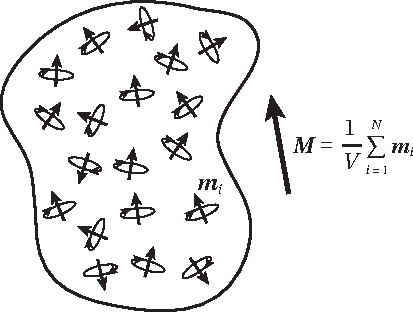
\includegraphics[]{magnetics/figures/magnetization.pdf}
    \caption{Magnetization is the sum of all magnetic moments within a body that give rise to an average magnetization. Magnetization is analogous to density for mass, except that it is a vector quantity.}
    \label{fig:magnetization}
\end{figure}

\subsection{The $B$-field and $H$-field}

There are two quantities that are often referred to as the magnetic field, $\vb{B}$ and $\vb{H}$. We will discuss their relationship shortly, but it is useful to clarify the terminology first, as it can be a source of confusion even among practitioners.

Historically, both $\vb{B}$ and $\vb{H}$ have been called the magnetic field. However, in most geophysical contexts, $\vb{B}$ is what is meant. The quantity $\vb{B}$ is also referred to as the \emph{magnetic induction} or \emph{magnetic flux density}, while $\vb{H}$ is known as the \emph{magnetic field strength} or \emph{magnetic field intensity} \citep{Purcell1985}.

In this chapter, unless otherwise noted, we will use the term \emph{magnetic field} to refer to $\vb{B}$, as this is the quantity that is measured in magnetic surveys. The field $\vb{H}$ will be introduced as the applied or ambient field used to describe how materials become magnetized. While their names may lead to confusion, their physical meanings are quite distinct. The definition of each of these fields is as follows:
\begin{description}
    \item [magnetic flux density, $\vb{B}$,] represents the total magnetic field, including contributions from both external sources and magnetized materials; and
    \item [magnetic field intensity, $\vb{H}$,] represents the applied or ambient magnetic field that drives the magnetization of materials.
\end{description}
In geophysical applications, $\vb{B}$ is the observable quantity, while $\vb{H}$ is used to describe how materials become magnetized.

The two fields are related by
\begin{equation}
    \vb{B} = \mu_0 (\vb{H} + \vb{M}),
\end{equation}
or equivalently,
\begin{equation}
    \vb{H} = \frac{1}{\mu_0}\vb{B} - \vb{M}.
\end{equation}
This relationship shows that the presence of magnetic materials modifies the total magnetic field.

\subsection{Induced magnetization (primary approximation)}

In many geological situations, the magnetization of a material is approximately proportional to the ambient magnetic field,
\begin{equation}
    \vb{M} = \chi \vb{H},
    \label{eq-sus}
\end{equation}
where $\chi$ is the (dimensionless) magnetic susceptibility introduced in the previous section.

Here, $\vb{H}$ represents the Earth's magnetic field, which has a typical magnitude of order $10^4$--$10^5$ \si{A.m^{-1}}. This observation implies that induced magnetization is controlled directly by susceptibility and the strength of the ambient field.

Substituting Equation~\ref{eq-sus} into the previous expression gives
\begin{equation}
    \vb{B} = \mu_0 (1+\chi)\vb{H} = \mu \vb{H},
\end{equation}
where $\mu = \mu_0 (1+\chi)$ is the magnetic permeability.

For most geological materials, $\chi \ll 1$, so $\mu \approx \mu_0$. As a result, variations in magnetic fields are controlled primarily by magnetization rather than changes in permeability.

Under the induced magnetization approximation:
\begin{itemize}
    \item magnetization is aligned with the Earth's magnetic field,
    \item its magnitude is proportional to susceptibility,
    \item anomaly geometry is controlled mainly by the shape of the source.
\end{itemize}
This approximation is the standard assumption used in many magnetic interpretations and forward models.

\subsection{Remanent magnetization (limitations of the approximation)}

In addition to induced magnetization, rocks may carry a remanent magnetization that reflects a past magnetic field. In general,
\begin{equation}
    \vb{M} = \vb{M}_{\mathrm{induced}} + \vb{M}_{\mathrm{remanent}}.
\end{equation}

Remanent magnetization may differ in both magnitude and direction from the present-day Earth's field. When it is significant, it can produce anomalies that deviate from the induced-only assumption.  In particular:
\begin{itemize}
    \item anomaly maxima may be displaced from the source,
    \item anomaly shapes may become asymmetric,
    \item transformations such as reduction to the pole may be inaccurate.
\end{itemize}

Despite these limitations, induced magnetization is often assumed as a first-order approximation. The origin and stability of remanent magnetization will be discussed in detail in the Paleomagnetism (Chapter~\ref{ch:paleomag}).  In practice, this is why magnetic modelling and inversion are commonly expressed in terms of susceptibility rather than magnetization, even though magnetization is the quantity that directly generates the magnetic field.


\section{Magnetic Properties of Rocks and Minerals}

Magnetic anomalies differ from gravity anomalies in one crucial respect: the sources are not ubiquitous. Most rocks contain little magnetic material, and the magnetic response is often controlled by trace amounts of specific minerals. As a result, magnetic anomalies are highly sensitive to mineralogy and alteration rather than bulk composition.

In this chapter, we will primarily assume that magnetization is induced and aligned with the Earth's magnetic field. This assumption greatly simplifies interpretation and is often reasonable, but it is not always valid. We will return to its limitations in later sections and in the Paleomagnetism chapter.

\subsection{Magnetic minerals and trace-element control}

The elements iron (Fe), nickel (Ni), and cobalt (Co) are magnetic, as are many of their oxides.  Iron oxides are the dominant source of magnetism, whereas Ni and Co are generally negligible because they are often orders of magnitude less abundant than Fe.  However, ores of Ni, and Co as well as in mafic and ultramafic rocks high in olivine, serpentinized peridotites, and komatiites may be sufficiently high in Ni that it contributes to the bulk magnetism, though still generally less than Fe.

In most crustal rocks, iron oxides, particularly iron--titanium oxides are the dominant magnetic minerals because they are widely distributed and exhibit a broad range of magnetic behaviours (Figure~\ref{fig:fetiox}).

Fe--Ti oxide minerals form solid-solution series, most importantly:
\begin{itemize}
    \item titanomagnetite, the magnetite--ulv\"ospinel series, and
    \item titanohematite, the hematite--ilmenite series.
\end{itemize}
Magnetic properties vary continuously along these series. For example, increasing Ti content in magnetite reduces both magnetization and Curie temperature. Consequently, even small compositional variations can strongly influence the magnetic behaviour of a rock.
\begin{figure}[hbt]
    \centerline{
        
\includegraphics[]{magnetics/figures/Fe_Ti_oxide_ternary.eps}
    }
    \caption{Compositions of common Fe--Ti oxides with solid solutions and the variations in Curie temperature with composition.}
    \label{fig:fetiox}
\end{figure}

An important geological example is provided by oceanic crust. Basalt formed at mid-ocean ridges commonly contains titanomagnetite, which is the primary carrier of magnetization in the oceanic lithosphere. As these rocks cool, they acquire a remanent magnetization aligned with the Earth's magnetic field at that time. This process is responsible for the linear magnetic anomaly patterns observed on the seafloor (discussed further in Chapter~\ref{ch:paleomag}).

Magnetic mineralogy can also be strongly modified by alteration. For example, at subduction zones and along oceanic faults, hydrothermal alteration of ultramafic rocks (serpentinization) can produce significant quantities of magnetite. This process can enhance magnetic anomalies in regions that would otherwise be only weakly magnetic.

In continental crust, magnetite and hematite are the dominant magnetic minerals. Their relative abundance depends strongly on the oxidation state of the crust. Magnetite typically dominates under reducing conditions, whereas hematite becomes more stable under oxidizing conditions, particularly in the middle and lower crust. This variation influences both the strength and character of magnetic anomalies in continental settings.

These minerals are generally in low abundance.  Hence, magnetic properties are often controlled by accessory mineral phases. A rock containing a small amount of magnetite may produce a stronger magnetic response than a rock composed primarily of weakly and non-magnetic minerals.

\subsection{Magnetic behaviour and susceptibility}

There is no universal mixing law for susceptibility because it depends not only on mineral proportions, but also on grain size, shape, and crystallographic orientation. As a result, susceptibility can vary by many orders of magnitude, even within a single rock type.

Magnetic susceptibility ($\chi$) describes how strongly a material becomes magnetized in response to an applied magnetic field.  It is a bulk property of rocks, but unlike density, susceptibility is not a universal property of matter and can vary over many orders of magnitude.  Materials can be classified according by their magnetic behaviour:
\begin{itemize}
    \item \textbf{Diamagnetic}: very weak, negative susceptibility (e.g., quartz, salt).
    \item \textbf{Paramagnetic}: small, positive susceptibility (common in many silicates).
    \item \textbf{(Ferri)magnetic}: large susceptibility and strong magnetization (e.g., magnetite, pyrrhotite).
\end{itemize}
In most rocks, diamagnetic and paramagnetic contributions are small. The bulk susceptibility is therefore dominated by ferrimagnetic minerals, even when they are present only in trace amounts.

At greater depths, the Earth's mantle is composed primarily of silicate minerals such as olivine and pyroxene, which are paramagnetic. As a result, the mantle contributes only weakly to magnetic anomalies. Most observed crustal-scale magnetic signals therefore originate within the crust, where ferrimagnetic minerals are present.

Representative values of susceptibility for common rocks and minerals are given in Table~\ref{tab-chi}.
\begin{table}
    \centering
    \begin{threeparttable}
    \caption{Table of rock and mineral susceptibilities.}
    \label{tab-chi}
    \begin{tabular}{lc}
        \toprule
        \textbf{Rock Type} & 
        \textbf{Susceptibility Range} \\
        \midrule
        dolomite (pure)   & -12.5 to +44 \\
        dolomite (impure) & 20000 \\
        limestone         & 10 to 25000 \\
        sandstone         & 0 to 21000  \\
        shale             & 60 to 18600 \\
        schist            & 315 to 3000 \\
        slate             & 0 to 38000 \\
        gneiss            & 125 to 25000 \\
        serpentenite      & 3100 to 75000 \\
        rhyolite          & 250 to 37700 \\
        granite           & 10 to 65 \\
        granite (w/ magnetite) & 20 to 50000 \\
        pegmatite         & 3000 to 75000 \\
        basalt            & 500 to 182000 \\
        gabbro            & 800 to 76000 \\
        peridotite        & 95500 to 196000 \\
        hematite          & 420 to 38000 \\
        magnetite         & 70000 to $2 \times 10^{7}$ \\
        ilmenite          & 314000 to $3.8 \times 10^{6}$ \\
        pyrite            & 50 to 5000 \\
        pyrrhotite        & 1250 to $6.3 \times 10^{6}$ \\
        chalcopyrite      & 400 \\
        ice               & -9 \\
        salt              & -10 \\
        graphite          & -80 to -200 \\
        \bottomrule
    \end{tabular}
    \begin{tablenotes}
        \item From \citet{Reynolds1997} pg. 127.
    \end{tablenotes}
    \end{threeparttable}
\end{table}
Several important observations follow:
\begin{itemize}
    \item Susceptibility can be zero or even negative (diamagnetic materials such as salt or ice).
    \item Variability within a rock type often exceeds differences between rock types.
    \item Small amounts of highly magnetic minerals (e.g., magnetite) dominate bulk behaviour.
\end{itemize}

A key implication is that magnetics is often controlled by accessory minerals. A granite containing a fraction of a percent of magnetite may produce a stronger anomaly than a mafic rock lacking magnetite.  Because few minerals are magnetic and those that are, are found in trace amounts.  

Chemical alteration further modifies magnetic properties. Processes such as oxidation, exsolution, and serpentinization can create or destroy magnetic minerals. The formation of magnetite during hydrothermal alteration of oceanic mantle (serpentinization) can enhance magnetic anomalies, 
\[
    6\underbrace{\ce{(Mg,Fe)2SiO4}}_{\text{olivine}} + 7\ce{H2O} \rightarrow
    3\underbrace{\ce{(Mg,Fe)3(Si_2O_5(OH))4}}_{\text{serpentine}} +
    \underbrace{\ce{Fe3O4}}_{\text{magnetite}} + \ce{H2} .
\]
Another example includes the exsolution of titanomagnetite during cooling can change magnetic minerals,
\[
    \underbrace{\ce{Fe_{3-x}Ti_xO4}}_{\text{titanomagnetite}} \rightarrow
    \underbrace{\ce{Fe3O4}}_{\text{magnetite}} +
    \underbrace{\ce{FeTiO3}}_{\text{ilmenite}} + \text{intermediate~spinels} .
\]
Near earth's surface, oxidation to hematite may weaken or modify magnetic signals
\[
    4\underbrace{\ce{Fe3O4}}_{\text{magnetite}} + \ce{O2} \rightarrow
    6\underbrace{\ce{Fe2O3}}_{\text{hematite}} .
\]
Because of this sensitivity, magnetic data are often used as a proxy for alteration patterns, particularly in mineral exploration.

\subsection{Curie temperature}

Magnetic minerals can sustain spontaneous magnetization only below a critical temperature known as the \emph{Curie temperature} ($T_C$). Above this temperature, thermal agitation disrupts magnetic ordering and the material becomes paramagnetic, losing any permanent magnetization.  Curie temperature is therefore a fundamental property that determines whether a mineral can carry a magnetic signal.  Representative values for common magnetic minerals are given in Table~\ref{tab-curie}.
\begin{table}
    \centering
    \begin{threeparttable}
    \caption{Table of common magnetic minerals and Curie temperature.}
    \label{tab-curie}
    \begin{tabular}{lcc}
        \toprule
        Mineral &
        Composition & 
        $T_{\si{C}}$ (\si{^\circ C}) \\
        \midrule
        iron            & $\alpha$\ce{Fe}          & 765 \\
        magnetite       & \ce{Fe3O4}               & 580 \\
        hematite        & $\alpha$\ce{Fe2O3}       & 675 \\
        maghemite       & $\gamma$\ce{Fe2O3}       & 590 to 675 \\
        titanomagnetite & \ce{Fe2.7Ti0.3O4}        & 350 \\
        {}              & \ce{Fe2.4Ti0.6O4}        & 150 \\
        goethite        & $\alpha$\ce{FeO(OH)}     & 120 \\
        pyrrhotite      & \ce{Fe7S8}               & 320 \\
        greigite        & \ce{Fe3S4}               & $\sim$330 \\
        \bottomrule
    \end{tabular}
    \begin{tablenotes}
        \item From {\citet{Dunlop&Ozdemir1997}} p. 51.
    \end{tablenotes}
    \end{threeparttable}
\end{table}

Curie temperature varies significantly between minerals and within mineral series. For example, titanomagnetite shows a strong decrease in $T_C$ with increasing titanium content, consistent with Figure~\ref{fig:fetiox}.  From a magnetic perspective, heating a rock above its Curie temperature will erase any prior magnetization. Upon cooling, the rock may acquire a new magnetization depending on the magnetic field at that time.

We will later return to the implications of Curie temperature at the crustal scale, where it provides a link between magnetic data and temperature structure.

\subsection{Induced and remanent magnetization (conceptual overview)}

There are two sources of magnetization: (1) induced magnetization is proportional to the present-day Earth's magnetic field and is controlled by susceptibility; and (2) remanent magnetization reflects a magnetic field that existed in the past and is retained by the rock.  The total magnetization of a rock can be expressed as the sum of these components,
\begin{equation}
    \coreeq
    \mathbf{M} = \mathbf{M}_{\mathrm{induced}} + \mathbf{M}_{\mathrm{remanent}}.
\end{equation}

In many magnetic surveys, it is assumed that induced magnetization dominates and is aligned with the Earth's field. This approximation simplifies interpretation and underlies many standard processing methods. However, this is not always accurate.

The total magnetization of a rock is the sum of induced and remanent components. The relative importance of these is commonly expressed using the K\"onigsberger ratio,
\begin{equation}
Q = \frac{|\mathbf{M}_{\mathrm{remanent}}|}{|\mathbf{M}_{\mathrm{induced}}|}.
\end{equation}
Typical values include:
\begin{itemize}
    \item $Q < 1$: sedimentary and many metamorphic rocks,
    \item $Q \approx 1$: slowly cooled igneous and regional metamorphic rocks,
    \item $Q \sim 10$: volcanic rocks,
    \item $Q \sim 30$--40: rapidly quenched basalts (e.g., oceanic crust).
\end{itemize}

Many of these minerals can acquire a permanent magnetization that is retained so long as the temperature remains below the Curie temperature. Above $T_C$, thermal agitation destroys long-range magnetic ordering and the material becomes paramagnetic.

For magnetic surveys, the details of how remanent magnetization is acquired are usually less important than its magnitude and direction.  When $Q$ is large, remanent magnetization may dominate the observed anomaly and produce directions that differ significantly from the Earth's present-day field.  This is one of the primary sources of ambiguity in magnetic interpretation and will be revisited later.

The origin and stability of remanent magnetization are central topics in paleomagnetism and will be discussed in detail in the Paleomagnetics chapter (Chapter~\ref{ch:paleomag}).



5. Magnetic Sources and Canonical Models
This parallels gravity, but with a clear warning label.
5.1 Dipoles and prisms
- Direction matters
- Source-anomaly offset
- Comparison to gravity bodies
- Mostly as-is
5.2 Geometry vs direction
- Why magnetics is harder to “eyeball”
- Latitude dependence
- Non-intuitive anomaly shapes
- New interpretive emphasis

\section{Theory}

\subsection{Monopole versus Dipole}

In our discussion on gravity, we described the potential due to mass.  We only have positive masses which create gravitational fields.  The fields are always directed towards the center of mass and are radially symmetric.  As a result, the equipotential surfaces form spheres about the source.  This behaviour can be described as a monopole.

In magnetism, however, monopoles do not exist (at least so far as we currently know---the search goes on).  The processes which generate magnetic fields result in dipolar fields: fields that are axially symmetric (symmetric about a single axis), but vary with orientation.  An example of monopole and dipole fields are shown in Fig.~\ref{fig:poles}. So, unlike gravity, magnetics introduces an additional complexity: the direction of magnetization plays a fundamental role in determining the observed field.

\begin{figure}[hbt]
    \centering
    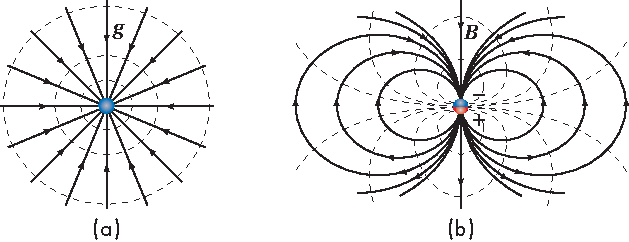
\includegraphics[]{magnetics/figures/poles.pdf}
    \caption{Field lines (solid) and equipotential surfaces (dashed) due to a (a) monopole and (b) dipole.}
    \label{fig:poles}
\end{figure}

This distinction is fundamental for interpretation. In gravity, anomaly shapes are largely controlled by geometry. In magnetics, the dipolar nature of the field introduces an additional dependence on direction, which makes anomaly shapes more complex and less intuitive.

\subsection{Dipolar Field}

\subsubsection{Magnetic Potential}

There are multiple ways to derive the field due to a dipole. One involves modeling two current loops, and while more technically accurate, it is more cumbersome. A simpler conceptual approach is to consider two monopoles of equal and opposite sign separated by a small distance. Although magnetic monopoles are a useful conceptual tool, the fundamental source of magnetic fields is the dipole. A dipole may be viewed as two equal and opposite poles separated by a small distance (Figure~\ref{fig:dipole}), or equivalently as a small current loop.

Using superposition,
\begin{equation*}
    V(P) = V_1(P) + V_2(P),
\end{equation*}
we examine two monopoles of opposite sign and separated by a small distance, $\Delta z$ (Fig.~\ref{fig:dipole}),
\begin{equation*}
    V(P) = -[V_1(P + \Delta z) - V_1(P)] .
\end{equation*}

\begin{figure}[hbt]
    \centering
    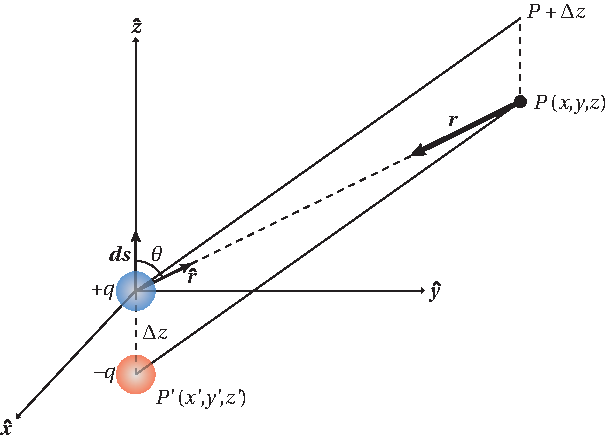
\includegraphics[]{magnetics/figures/two_poles.pdf}
    \caption{Two monopoles of opposite sign in proximity result in a dipolar field. After \citet{Blakely1995}.}
    \label{fig:dipole}
\end{figure}

Taking the limit as the separation becomes small,
\begin{equation*}
    V(P) = - \Delta z \dv{V_1(P)}{z}.
\end{equation*}

Using the magnetic potential of a monopole,
\begin{align}
    U(P) &= G \frac{m}{r} \quad \text{(gravity)} \\
    V_1(P) &= \frac{\mu_0}{4 \pi} \frac{q}{r} \quad \text{(magnetics)},
\end{align}
we obtain
\begin{equation*}
    V(P) = - \frac{\mu_0}{4 \pi} q \Delta z \dv{}{z} \frac{1}{r}.
\end{equation*}

Generalizing to arbitrary orientation,
\begin{equation*}
    V(P) = - \frac{\mu_0}{4 \pi} q \dd{\vb{s}} \cdot \grad \frac{1}{r}.
\end{equation*}

Defining the dipole moment,
\begin{equation}
    \vb{m} = q \dd{\vb{s}},
\end{equation}
gives
\begin{equation}
    V(P) = -\frac{\mu_0}{4 \pi} \vb{m} \cdot \grad \frac{1}{r}.
\end{equation}

\subsubsection{Magnetic Field}

The magnetic field is obtained from the potential,
\begin{equation}
    \vb{B} = - \grad V.
\end{equation}

Applying the vector identity yields
\begin{equation}
    \vb{B}(r,\theta) = \frac{\mu_0}{4 \pi} \frac{m}{r^3}
    [3(\hat{\vb{m}} \cdot \hat{\vb{r}})\hat{\vb{r}} - \hat{\vb{m}}].
\end{equation}

This expression highlights two important features:

\begin{itemize}
    \item The field decays as $1/r^3$, more rapidly than gravity ($1/r^2$).
    \item The field depends explicitly on the orientation of the dipole.
\end{itemize}

The second point is particularly important: unlike gravity, the direction of the source affects the shape of the observed anomaly.

\subsection{From Dipoles to Magnetized Bodies}

Magnetized geologic bodies, while more complex in geometry, can be viewed as a collection of dipoles.  Taking an approach similar to gravity where we reformulated the equations to use density instead of mass, we will view bodies in terms of magnetization instead of dipole moments.  For a material with uniform magnetization $\vb{M}$, each small volume element behaves like a dipole with moment $\vb{m} = \vb{M} \dd{v}$.

Integrating over the body gives
\begin{equation}
    \vb{B} = - \frac{\mu_{0}}{4\pi} \nabla_{P} \int_{V} 
    \vb{M}(Q) \cdot \nabla_{Q} \frac{1}{r} \dd{v}.
    \label{eq-mag}
\end{equation}

While analogous to the gravitational field equation, the vector nature of magnetization with both magnitude and direction influence the magnetic field.

\subsection{Constitutive Relationship and Poisson Analogy}

In the induced magnetization approximation,
\begin{equation}
    \vb{M} = \chi \vb{H}.
\end{equation}

Substituting this into Equation~\ref{eq-mag} shows that the magnetic field is controlled by the spatial distribution of susceptibility, much like density in gravity.

The magnetic potential satisfies a Poisson-type equation,
\begin{equation}
    \laplacian V = \div \vb{M}.
\end{equation}

Under induced magnetization,
\begin{equation}
    \laplacian V = \div (\chi \vb{H}),
\end{equation}
which demonstrates that magnetic anomalies arise from spatial variations in susceptibility and from the direction of the inducing field.

This is a key distinction from gravity: even when susceptibility is the parameter being modeled, the resulting field depends on both geometry and field direction.

\subsection{Conceptual Representations of Magnetic Fields}

There are three equivalent conceptual models:

\begin{enumerate}
    \item Magnetic poles
    \item Current loops
    \item Uniformly magnetized bodies
\end{enumerate}

\begin{figure}[hbt]
  \centering
  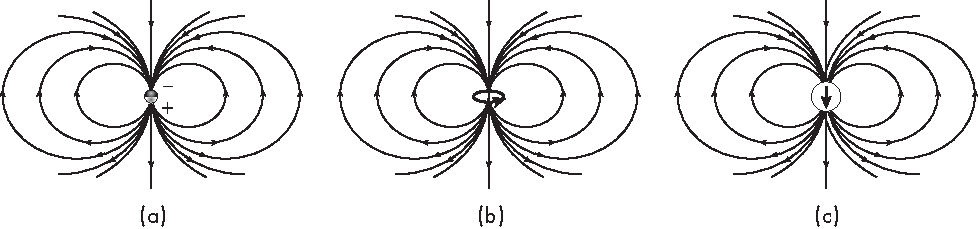
\includegraphics[]{magnetics/figures/magnetic_fields.pdf}
  \caption{Conceptual representations of magnetic fields.}
  \label{fig:magfields}
\end{figure}

These representations all produce equivalent dipole fields and are used interchangeably.

\subsection{Geometry versus Direction}

In gravity, anomaly shapes are largely controlled by source geometry. In magnetics, both geometry and direction matter.  And while all magnetic models reduce to dipoles at sufficient distance, the observable anomalies differ strongly from gravity.

As shown in Fig.~\ref{fig:monodi},
\begin{figure}[hbt]
  \centerline{
    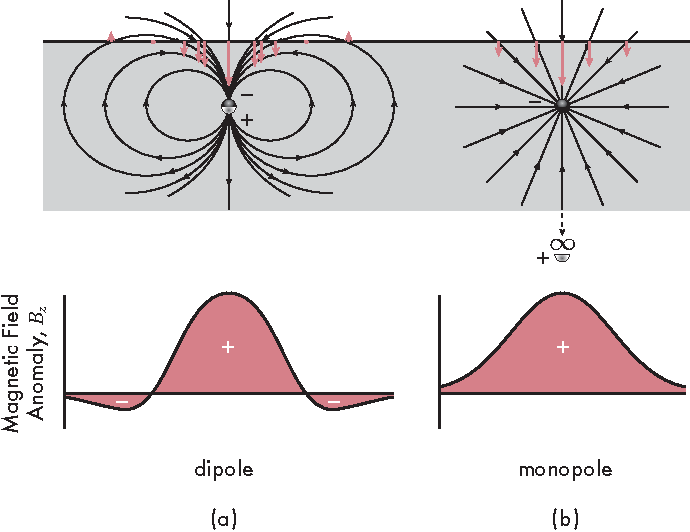
\includegraphics[]{magnetics/figures/monodipole.pdf}
  }
  \caption{Dipole versus monopole responses.}
  \label{fig:monodi}
\end{figure}

\begin{itemize}
    \item Magnetic anomalies are typically asymmetric.
    \item The anomaly peak is often offset from the source.
    \item The anomaly shape depends on the direction of the Earth's field (i.e., latitude).
\end{itemize}

This directional dependence makes magnetic anomalies significantly more difficult to interpret by inspection than gravity anomalies.

\emph{Key point:} Magnetic anomalies are controlled by both the geometry of the source and the direction of magnetization. This dual dependence is the primary reason magnetics is less intuitive than gravity.

\ntextbox{Practical perspective}{
    Magnetics is often described as more complex than gravity because magnetization is a vector quantity and anomaly shapes depend on direction. However, this does not necessarily make magnetic modelling more difficult.

    In practice, magnetized bodies are represented using simple geometric elements (e.g., prisms), and their fields are computed by superposition, just as in gravity. Once the direction of magnetization is specified or approximated (for example, using reduction to the pole), magnetic modelling becomes comparable in complexity to gravity modelling.

    Magnetics also has two important advantages for exploration:
    \begin{itemize}
        \item Magnetic anomalies are largely confined to the crust because most mantle temperatures exceed the Curie temperature.
        \item Magnetic fields decay more rapidly with distance ($B \propto 1/r^3$) than gravitational fields ($g \propto 1/r^2$), producing sharper anomalies for the same source.
    \end{itemize}
}{core}\label{box:mag_adv}

\subsection{Magnetic Field of a Rectangular Prism}

A rectangular prism with uniform magnetization provides one of the most important canonical models in applied magnetics. It forms the basis for most forward modelling and inversion methods, where complex bodies are represented as collections of simple elements.

Consider a rectangular prism bounded by
\[
x_1 \le x \le x_2,\quad
y_1 \le y \le y_2,\quad
z_1 \le z \le z_2,
\]
with observation point at $(x,y,z)$ and magnetization $\vb{M} = (M_x, M_y, M_z)$.

Define shifted coordinates
\[
X_i = x - x_i,\quad 
Y_j = y - y_j,\quad 
Z_k = z - z_k,
\]
where $i,j,k \in \{1,2\}$.

Also define
\[
r_{ijk} = \sqrt{X_i^2 + Y_j^2 + Z_k^2}.
\]

The magnetic field components can be written as

\begin{align}
B_x &= \frac{\mu_0}{4\pi} \sum_{i,j,k} (-1)^{i+j+k}
\bigg[
M_x \tan^{-1}\left( \frac{Y_j Z_k}{X_i r_{ijk}} \right)
- M_y \ln (r_{ijk} + Z_k)
- M_z \ln (r_{ijk} + Y_j)
\bigg],
\\
B_y &= \frac{\mu_0}{4\pi} \sum_{i,j,k} (-1)^{i+j+k}
\bigg[
M_y \tan^{-1}\left( \frac{X_i Z_k}{Y_j r_{ijk}} \right)
- M_x \ln (r_{ijk} + Z_k)
- M_z \ln (r_{ijk} + X_i)
\bigg],
\\
B_z &= \frac{\mu_0}{4\pi} \sum_{i,j,k} (-1)^{i+j+k}
\bigg[
M_z \tan^{-1}\left( \frac{X_i Y_j}{Z_k r_{ijk}} \right)
- M_x \ln (r_{ijk} + Y_j)
- M_y \ln (r_{ijk} + X_i)
\bigg].
\end{align}

These expressions show that the magnetic field is computed as a sum over the eight corners of the prism, with alternating signs. This structure is analogous to the Talwani formulation for gravity, where the field is expressed in terms of contributions from the corners of a polygon.

The logarithmic and arctangent terms arise from the integration of dipole contributions over the volume of the body.

Care must be taken in evaluating the logarithmic and arctangent terms near singularities (e.g., when $X_i$, $Y_j$, or $Z_k$ approach zero). In practice, stable numerical implementations use the two-argument arctangent function and avoid evaluating expressions exactly on prism boundaries.

A key distinction from gravity is that the magnetic field depends explicitly on the components of the magnetization vector $(M_x, M_y, M_z)$. As a result:
\begin{itemize}
    \item both geometry and direction control the anomaly,
    \item changing magnetization direction can strongly alter anomaly shape,
    \item identical bodies can produce very different anomalies depending on magnetization.
\end{itemize}

Under the induced magnetization assumption,
\begin{equation}
    \vb{M} = \chi \vb{H}_0,
\end{equation}
where $\vb{H}_0$ is the Earth's magnetic field.

In this case, the direction of $\vb{M}$ is known, and the problem reduces to determining the effect of the prism geometry and susceptibility.

This represents a first-order approximation. If remanent magnetization is significant, the direction of $\vb{M}$ must be specified independently.

Although these expressions appear more complex than their gravity equivalents, they are straightforward to evaluate numerically. In practice, complex bodies are modeled by dividing the subsurface into many prisms and summing their contributions.

Under simplifying assumptions such as induced magnetization or reduction-to-the-pole, magnetic modelling becomes comparable in difficulty to gravity modelling.


\section{Intuitive Field Shapes and Source Geometry}

The formal development of magnetic fields in the previous section provides a complete mathematical description of magnetic sources. However, interpretation often relies on developing an intuitive understanding of how different source geometries produce characteristic anomaly shapes.

In this section, we examine simplified bodies and build intuition by viewing magnetized objects as collections---\emph{superposition}---of dipoles. This perspective allows us to anticipate the qualitative form of magnetic anomalies without performing detailed calculations.

\subsection{A narrow, vertically magnetized dike}

Consider a narrow vertical dike with uniform magnetization directed vertically. If the width of the dike is small compared to its depth extent, the body behaves approximately as a single dipole.

In this case:
\begin{itemize}
    \item the anomaly is symmetric about the center of the body,
    \item a single peak (or trough) is observed,
    \item the anomaly resembles the response of an isolated dipole.
\end{itemize}

As the depth extent of the dike increases, the anomaly becomes increasingly dipole-like. This reflects the fact that the distant portions of the body contribute less strongly to the field, and the response is dominated by the bulk moment of the source.

\subsection{A wide dike or sill: superposition of dipoles}

Now consider increasing the width of the dike (or equivalently, a sill). The body can be viewed as a collection of dipoles distributed along a horizontal line.

To understand the resulting anomaly, consider the vertical component of the magnetic field, $B_z$, at different observation points.

\paragraph{Observation above the center}

At a point directly above the center of the body:

\begin{itemize}
    \item the dipole directly beneath the observation point contributes the largest positive $B_z$,
    \item nearby dipoles also contribute positively, but less strongly because their field lines spread outward and include horizontal components,
    \item dipoles further away eventually contribute negatively, as their field lines intersect the observation point from below at an opposing orientation.
\end{itemize}

The combined effect is a relatively high value of $B_z$ at the center, but lower than the peak values observed near the edges of the body due to the influence of these distant negative contributions.

\paragraph{Observation near the edge}

At a point near the edge of the body:

\begin{itemize}
    \item dipoles to one side of the observation point contribute positively,
    \item dipoles on the opposite side include both positive and negative contributions, but the geometry results in a net enhancement,
    \item the balance of contributions leads to a maximum in $B_z$ near the edge of the body.
\end{itemize}

\paragraph{Observation beyond the edge}

Beyond the edge of the body:

\begin{itemize}
    \item only dipoles on one side contribute,
    \item these contributions become increasingly negative with distance,
    \item the field decays toward zero from the negative side.
\end{itemize}

This behaviour is mirrored on both sides of the body, resulting in a symmetric anomaly with:
\begin{itemize}
    \item peaks near the edges,
    \item a lower-amplitude plateau over the center,
    \item decay to zero at large distances.
\end{itemize}

\subsection{Summary: width and depth effects}

From these examples, several general principles emerge:

\begin{itemize}
    \item Increasing depth extent makes a body appear more dipole-like.
    \item Increasing lateral extent produces broader anomalies with edge enhancements.
    \item The observed field at any point is the result of competing positive and negative contributions from different parts of the source.
\end{itemize}

These effects are a direct consequence of the dipolar nature of magnetic fields.

\subsection{Effect of magnetization direction}

The examples above assumed vertical magnetization. If the direction of magnetization is changed, the relative contributions from different parts of the body also change.

For a single dipole:
\begin{itemize}
    \item the direction of $\vb{M}$ controls the orientation of the field,
    \item the position of anomaly maxima shifts relative to the source,
    \item the anomaly becomes asymmetric.
\end{itemize}

For extended bodies, this effect is amplified:
\begin{itemize}
    \item peaks shift laterally,
    \item positive and negative lobes become unequal,
    \item anomaly shapes depend strongly on latitude through the Earth's field direction.
\end{itemize}

\noindent {\bf Key observation.} Magnetic anomalies cannot be understood purely in terms of geometry. Even for simple bodies, the distribution of positive and negative contributions depends on both the shape of the source and the direction of magnetization.

\section{Measuring the Magnetic Field}

Magnetic surveys measure the total magnetic field, which includes contributions from both the Earth's main field and local variations caused by magnetized structures in the crust. In practice, the measured field must be corrected to isolate these local variations (deviations), known as magnetic anomalies---the primary target of interpretation.

The Earth's magnetic field is dominated by a large-scale component generated in the core, which varies smoothly in space and time. Superimposed on this are smaller-scale contributions from the crust, which are the focus of magnetic exploration.

Magnetic data processing is generally simpler than gravity because fewer corrections are required. The main steps are:
\begin{itemize}
    \item removal of temporal variations (diurnal correction),
    \item removal of the Earth's main field (IGRF),
    \item optional separation of regional and residual components.
\end{itemize}

\subsection{Magnetometers}

The commonly used varieties in use today are alkali vapor (optically pumped) magnetometers and proton precession magnetometers.  These types can be hand-held, or mounted to a moving vehicle (car, airplane, ship).  Alkali vapor and proton precession magnetometers measure the total magnetic field strength,
\[
T = |\vb{B}|,
\]
but not its direction.

For total field magnetometers, it is common to express anomalies as the projection of the magnetic field onto the direction of the regional field, $\hat{\vb{F}}$. The total field anomaly is then approximated as
\[
    \delta T = \hat{\vb{F}} \cdot \delta \vb{B},
\]
which, using Equation~\ref{eq-mag}, can be written as
\[
    \delta T = - \frac{\mu_{0}}{4\pi} \hat{\vb{F}} \cdot \nabla_{P}
    \int_{V} \vb{M} \cdot \nabla_{Q}
    \frac{1}{r} dv.
\]

Also commonly used for airborne, shipborne, satellite, and base station measurements are flux gate magnetometers.  Flux gates measure the field strength in one direction so they are generally used in combination of three to measure the vector field magnitude in three orientations.  This vector measurement can be highly advantageous as it can aid in interpreting and modeling anomalies.

\subsection{The Earth's main field (IGRF)}

The dominant contribution to the measured magnetic field is the Earth's main field, generated by dynamo processes in the liquid outer core. This field is smooth at the scale of most surveys and varies gradually as a function of latitude, longitude, and time.

The International Geomagnetic Reference Field (IGRF) provides a standard model of the Earth's main field based on spherical harmonic expansions. It is periodically updated to account for secular variation.

The IGRF defines, at any location and time:
\begin{itemize}
    \item the total field strength,
    \item the inclination (dip angle),
    \item the declination (horizontal direction).
\end{itemize}

These parameters are used to define the direction of the inducing field $\vb{H}_0$ in modelling.

\begin{figure}[hbt]
  \centering
  %\includegraphics[]{magnetics/figures/igrf_global.pdf}
  \caption{Global distribution of the Earth's magnetic field strength (IGRF model).}
  \label{fig:igrf}
\end{figure}

\subsubsection{Latitude and Longitude Corrections}

The Earth's main magnetic field is typically removed using a reference model such as the IGRF.  This correction produces the residual field, which isolates contributions from crustal magnetization.

For small surveys, this correction may be approximated by subtracting a constant value or may not be done at all. For larger surveys, a spatially varying reference field is required, adjusting for spatial variations in latitude and longitude.

\subsection{Additional Corrections}

Very few corrections are necessary for magnetic data which makes data reduction significantly simpler than gravity.

\subsubsection{Diurnal Variations}

The Earth's magnetic field is warped by the solar wind, compressing magnetic field lines in the direction of the sun and stretching out the field lines away from the sun (Fig.~\ref{fig:solarwind}).  Additionally, the intensity of the solar wind varies due to normal solar processes causing the magnetic field to pulse as it pushes back.  The intensity of these pulsations and compression of field lines can be particularly large during solar storms.  However, we can account for these variations by continuously recording the magnetic field at a base station somewhere within or nearby the field site.
\begin{figure}[hbt]
  \centerline{
    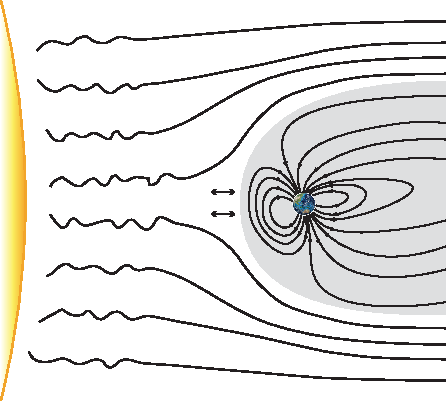
\includegraphics[]{magnetics/figures/solar_wind.pdf}
  }
  \caption{The Earth's magnetic field is distorted by the solar wind.}
  \label{fig:solarwind}
\end{figure}

\subsubsection{Altitude and Topography}

Because the magnetic field varies with height above the Earth's surface, small elevation differences can introduce variations in the measured field. These effects are typically small ($<0.03$~nT~m$^{-1}$) and are often neglected.

However, airborne surveys may be flown at different altitudes above the land surface.  In such cases, surveys can be combined only after adjusting one or both so that they approximate the same flight altitude.  Such adjustements are typically made using upward or downward continuation (Section~\ref{sec:continuation}).

The topographic correction is generally not applied, but may be necessary in some cases with significant topography and highly magnetized terranes (e.g., lava flows and intrusions).

\subsection{Magnetic Anomalies}

As discussed previously, the magnetic field due to a body can be viewed in terms of pole pairs, currents or uniform magnetization.  As seen from the equations for a dipole, the observed magnetic field from a body depends not only upon the distance from the body, but also the azimuth.  In the case of buried structures or targets, the orientation of magnetization may not be purely vertical or horizontal making the observed response asymmetric (Figure~\ref{fig:skew}).
\begin{figure}[hbt]
  \centerline{
    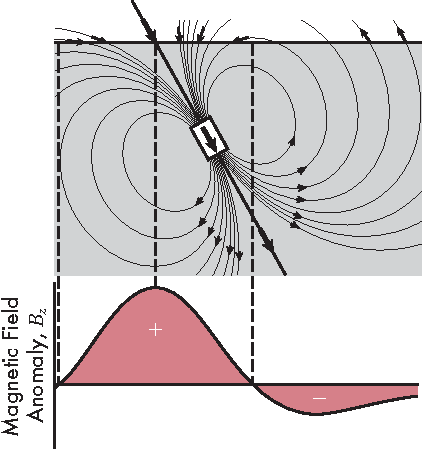
\includegraphics[]{magnetics/figures/skew_dipole.pdf}
  }
  \caption{The vertical component of a rotated dipole that is buried near the surface shows a highly asymmetric response.  Note that the orientation of the survey across the dipole would be different.}
  \label{fig:skew}
\end{figure}
The shape of the body and its extent also affect the observed response (Fig.~\ref{fig:nvw}).
\begin{figure}[hbt]
  \centerline{
    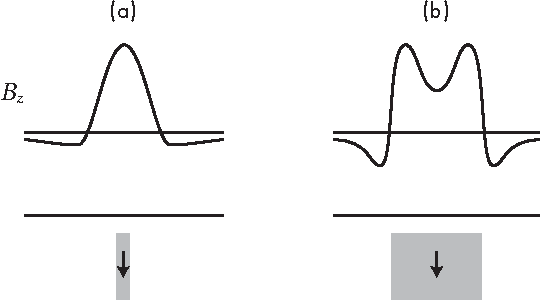
\includegraphics[]{magnetics/figures/narrow_vs_wide.pdf}
  }
  \caption{The vertical magnetic response of a (a) narrow and (b) wide body magnetized in the vertical direction.}
  \label{fig:nvw}
\end{figure}

\section{Regional residuals}

Whereas gravitational attraction results from the density structure of the Earth from the top of the atmosphere to the core, magnetic variations come from the core (Earth's field) and the lithosphere (remnant and induced magnetization).

Regional residuals for magnetics are removed much the same way as they are for gravity.  After removal of the main field (e.g., IGRF), remaining long-wavelength variations may still be present and can be separated using methods similar to those used in gravity.  For example, Upward continuation is commonly used to suppress shallow sources and emphasize regional trends, while downward continuation enhances shallow features but amplifies noise.  Fourier domain filtering is also widely used to separate regional and residual components.

\section{Transformations and Spectral Thinking}

Magnetic anomalies are strongly influenced by the direction of magnetization and the spatial distribution of sources. As a result, raw magnetic data can be difficult to interpret directly. A variety of transformations are therefore used to simplify anomaly shapes, enhance specific features, or extract information about source depth.

Many of these transformations are most naturally expressed in the Fourier domain, where operations such as filtering, differentiation, and continuation become simple algebraic manipulations. In this section, we focus on the physical meaning and practical implications of these transformations, leaving detailed derivations to the Fourier Transform chapter.

\subsection{Reduction to the Pole (RTP)}

The reduction to the pole transform is designed to simplify the interpretation of magnetic anomalies by transforming the observed field to the response that would be measured if both the Earth's magnetic field and the magnetization were vertical (i.e., inclination of $90^\circ$).
\begin{center}
    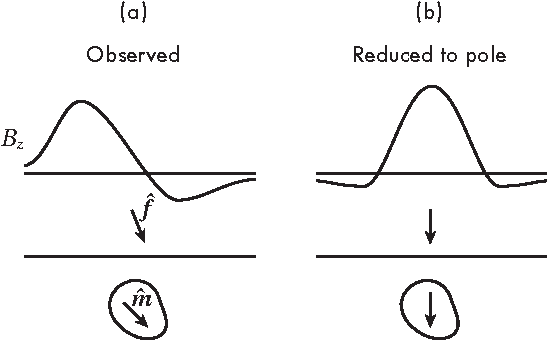
\includegraphics[]{magnetics/figures/reduced_to_pole.pdf}
    \captionof{figure}{The reduction to the pole transforms the observed Earth's field and magnetization orientations, $\vu{f}$ and $\vu{m}$, to the vertical.}
    \label{fig:rtpole}
\end{center}

Physically, the effect of RTP is to remove the directional dependence of the magnetic field. As a result, anomalies become more symmetric and their maxima are shifted closer to the source location. In this sense, RTP transforms magnetic data into something that more closely resembles gravity, where anomaly geometry is easier to interpret.

In the Fourier domain, RTP is implemented as a filter that depends on the direction of the Earth's field and the magnetization. The mathematical expression involves both amplitude and phase modification and is therefore sensitive to noise and numerical instability. (Details are provided in Box~\ref{box:rtp}.)

\ntextbox{Reduction to pole}{
    The reduction to pole transform is meant to simplify interpretation of magnetic maps by transforming the Earth's and magnetized field from the observed to vertical, 90$^\circ$ (Fig.~\ref{fig:rtpole}).
    \begin{center}
        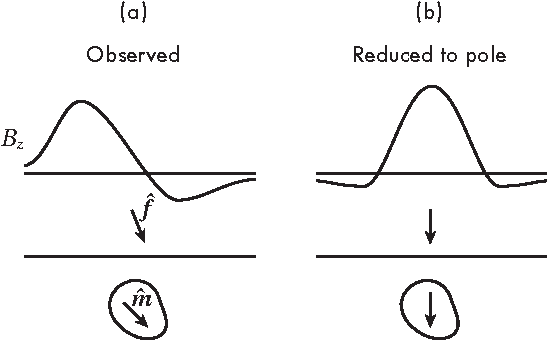
\includegraphics[]{magnetics/figures/reduced_to_pole.pdf}
        \captionof{figure}{The reduction to pole transforms the observed Earth's field and magnetization orientations, $\vu{f}$ and $\vu{m}$, to the vertical.}
        \label{fig:rtpole}
    \end{center}

    The reduction to pole transform is a Fourier domain technique given by
    \[
        \ft{\Delta T_{r}} = \ft{\psi_{r}} \ft{\Delta T},
    \]
    where $\ft{\psi_{r}} = \Theta_{m} \Theta_{f}$ and is related to the direction of magnetization, $\vu{m} = (\vu{m}_x,\vu{m}_y,\vu{m}_z)$, and the Earth's field direction, $\vu{f} = (\vu{f}_x,\vu{f}_y,\vu{f}_z)$, by
    \begin{eqnarray*}
        \Theta_{m} & = & \vu{m}_{z} 
            + i\frac{\vu{m}_x k_x + \vu{m}_y k_y}{|k|}, \\
        \Theta_{f} & = & \vu{f}_{z} 
            + i\frac{\vu{f}_x k_x + \vu{f}_y k_y}{|k|}.
    \end{eqnarray*}
    Both $\vu{m}$ and $\vu{f}$ are unit vectors.

    \noindent {\bf Pros:}
    \begin{itemize}
        \item Often helps identify the source of an anomaly by placing a peak over the center or edges.
    \end{itemize}
    {\bf Cons:}
    \begin{itemize}
        \item Only works when the remnant field is induced (i.e.\ magnetized at the same inclination as the Earth's present-day field).
        \item The transform is unstable at low latitudes ($\pm$10$^\circ$) due to the large rotation of inducing field; although, a mathematical fix is possible in some cases.
    \end{itemize}
}{aside}\label{box:rtp}

RTP performs well when several conditions are satisfied: the magnetization is primarily induced so that $\vb{M} \parallel \vb{H}_0$, the data are acquired at moderate to high magnetic latitudes, and the anomaly geometry is relatively simple.

However, it becomes unreliable when these assumptions break down. In particular:
\begin{itemize}
    \item significant remanent magnetization alters the direction of $\vb{M}$,
    \item low magnetic latitudes require large phase rotations,
    \item noise and limited data extent introduce instability.
\end{itemize}

At low latitudes in particular, the transformation becomes unstable because it requires large phase rotations of the data. Modified or stabilized versions of RTP exist, but care must always be taken in interpreting the results.

\emph{Key idea:} RTP attempts to remove directional complexity from magnetic data. When its assumptions are valid, it can make magnetics look much more like gravity.

\subsection{Continuation and Filtering (Conceptual View)}

Continuation and filtering are often used to emphasize features at different scales or depths.

\paragraph{Depth--wavelength relationship}

A fundamental principle in potential field methods is that:
\begin{center}
\emph{long wavelengths are associated with deeper sources, while short wavelengths are associated with shallow sources.}
\end{center}

This arises from the decay of potential fields with distance (e.g., $B \propto 1/r^3$ for dipoles). In the Fourier domain, this relationship becomes explicit through exponential weighting of different spatial frequencies.

Upward continuation smooths the field by preferentially attenuating short wavelengths. Because these short wavelengths are associated with shallow sources, the resulting field emphasizes deeper, more regional structure.

Downward continuation has the opposite effect, amplifying short-wavelength components and enhancing shallow features. However, this enhancement applies equally to signal and noise, making the process intrinsically unstable. Even small errors in the data can grow rapidly, limiting its practical use.

As a result, downward continuation is inherently unstable and must be used with caution.

\paragraph{Derivative and filtering operations}

All filtering operations involve a trade-off between resolution and stability. Enhancing high-frequency components can sharpen anomalies and improve edge detection, but it also amplifies noise. As a result, the effective resolution of filtered data is often controlled more by noise than by the underlying signal.

In practice, all such operations involve a trade-off between resolution and stability.

\emph{Key idea:} Filtering redistributes energy between spatial scales. Enhancing small features always comes at the cost of increased sensitivity to noise.

\subsection{Pseudo-gravity Transformation}

The pseudo-gravity transform attempts to convert a magnetic anomaly into an equivalent gravity anomaly under simplifying assumptions.

The motivation for this transformation comes from the formal similarity between gravitational and magnetic potentials. If both density and magnetization are constant within a body, the two fields are related through spatial derivatives.

In practice, the transformation is implemented as a Fourier-domain filter that converts the observed magnetic field into a pseudo-gravity response (Box~\ref{box:pseudogravity}).

\ntextbox{Pseudo-gravity}{
The pseudo-gravity transform attempts to take a magnetic anomaly and estimate the gravitational attraction.  If density and magnetization are constant, we can write the gravitational and magnetic potentials as
\begin{eqnarray*}
    U_{g}(P) & = & G \rho\int_{V} r^{-1} dv, \\
    U_{m}(P) & = & - \frac{\mu_0}{4\pi}\vb{M} \cdot \nabla_{P} \int_{V} r^{-1} dv.
\end{eqnarray*}
Note the similarity between the two potentials, we can show that 
\[
    U_{m}(P) = -\frac{\mu_0}{4\pi G \rho} \vb{M} \cdot \nabla_{P} U_{g}.
\]
Recall, $g = \nabla U_{g}$; therefore,
\[
    U_{m}(P) = -\frac{\mu_0 M g_{m}}{4\pi G \rho},
\]
where $g_{m}$ is the component of gravity in the direction of magnetization.  But we really care about the vertical component of $g$ just as we would observe from a gravity survey.  To find this, we have to return to the Fourier domain where it can be shown that
\[
    \ft{\Delta T_{psg}} = \ft{\psi_{psg}} \ft{\Delta T},
\]
where $\Delta T_{psg}$ is the pseudo-gravity derived from the total field and
\[
    \ft{\psi_{psg}} = \frac{4\pi G}{\mu_{0} |k| \Theta_{m} \Theta_{f}} \frac{\rho}{M}.
\]
The psuedo-gravity transform in this way is related to the reduction to pole shown earlier (i.e.\ $\ft{\psi_{psg}} = 4\pi G \mu_{0}^{-1} |k|^{-1} \ft{\psi_{r}}$).  As a result, the pseudo-gravity transform also suffers from numerical instability at low latitudes.

There is also a pseudo-magnetic transform that can be applied to observed gravity.  However, the pseudo-magnetic transformation can be unstable and is basically never used anyway.
}{aside}\label{box:pseudogravity}

The pseudo-gravity transform can provide a more intuitive representation of magnetic data because gravity anomalies are often easier to interpret geometrically. By reducing directional effects, the transform produces responses that resemble those of density variations, highlighting the density-like behaviour of magnetic sources and aiding qualitative interpretation.

These advantages must be balanced against important limitations. The transformation assumes a constant ratio of magnetization to density ($M/\rho$), which is rarely satisfied in heterogeneous crustal environments. It is also sensitive to errors in the assumed magnetization direction, and shares the same instability issues as reduction to the pole, particularly at low magnetic latitudes. As a result, pseudo-gravity is best used as a qualitative interpretive tool rather than a quantitative inversion method.

As a result, pseudo-gravity is best viewed as an interpretive aid rather than a quantitative transformation.

\subsection{Curie Depth (Spectral Perspective)}


Because most mantle minerals are paramagnetic and crustal minerals lose magnetization at elevated temperatures, the ability of the Earth to generate magnetic anomalies is largely restricted to relatively shallow regions containing ferrimagnetic minerals below the Curie temperature.

This depth can be estimated using spectral methods by examining the longest wavelengths present in the data. Under the assumption that deeper sources produce longer wavelengths, the low-wavenumber content of the magnetic field provides an estimate of the maximum depth of magnetization.

If we know the mineral the mineral responsible for the majority of magnetization of the crust, then we can assign a temperature to this depth based on the Curie temperature (Table~\ref{tab-curie}).  Identifying the variations in depth of this Curie isotherm allows us to estimate surface heat flow and geotherms.  While this may not be useful for small studies, it may be useful for identifying possible geothermal targets on a regional basis\ldots though in my experience the results do not match surface heat flow estimates all that well and should be used with caution.

Estimates of Curie depth provide a measure of the base of the magnetized crust. Where the dominant magnetic mineral is known, this depth can be related to thermal structure through its Curie temperature, offering insight into subsurface temperature distributions. As a result, Curie depth estimates are most useful at regional scales, where they can help identify large-scale thermal variations such as those associated with geothermal systems.

These interpretations rely on several simplifying assumptions. In particular, they require that a single magnetic mineral with a known Curie temperature dominates the magnetic signal, which is often not the case in heterogeneous crust. The method also depends on approximate relationships between wavelength and depth, introducing additional uncertainty. Furthermore, spectral estimates are sensitive to noise and the spatial extent of the data, which can significantly affect the reliability of the inferred depths.

Thus, Curie depth estimates should be interpreted as approximate and model-dependent.

\subsection{Why Fourier Space Matters (Preview)}

Many of the transformations discussed above are most naturally expressed in the Fourier domain.

In real space:
\begin{itemize}
    \item operations such as continuation or differentiation involve integrals,
    \item directional effects are difficult to isolate.
\end{itemize}

In Fourier space:
\begin{itemize}
    \item convolution becomes multiplication,
    \item derivatives become simple algebraic factors,
    \item directional filters (such as RTP) can be applied directly.
\end{itemize}

This makes Fourier methods computationally efficient and conceptually powerful.

\emph{Key idea:} Fourier space provides a natural framework for manipulating potential fields. Many operations that are complex in real space become simple, intuitive filters in the spectral domain.

\section{Non-Uniqueness and Ambiguity in Magnetics}

All potential field methods are inherently non-unique: many different subsurface models can produce the same observed field. However, magnetics departs from gravity in a fundamental way, as ambiguity arises not only from source geometry, but also from the direction and nature of magnetization.

In gravity, anomalies are controlled primarily by the geometry of density contrasts. In magnetics, the situation is more complex because magnetization is a vector quantity. A single body may produce very different anomalies depending on the direction of magnetization, leading to asymmetry in anomaly shapes and offsets between anomaly maxima and the true source location. Consequently, different combinations of geometry and magnetization direction can yield similar observed fields, making interpretation by inspection significantly more difficult than in gravity.

A further source of ambiguity arises from the distinction between induced and remanent magnetization. In many applications, it is assumed that magnetization is induced and aligned with the present-day Earth's magnetic field. While this assumption simplifies interpretation, it is not always valid. When remanent magnetization is present and significant, the direction of the total magnetization vector may differ substantially from that of the Earth's field. This can result in anomaly shapes that are inconsistent with induced-only models and can cause transformations such as reduction to the pole to fail or produce misleading results. Because remanent magnetization is often poorly constrained, it is difficult to separate its effects from those of geometry.

Magnetic data are frequently interpreted in terms of susceptibility, particularly under the assumption of induced magnetization. However, the observed field is produced by the total magnetization, not susceptibility alone. This introduces another level of ambiguity. A strong anomaly may reflect high susceptibility, strong remanent magnetization, or some combination of both. Similarly, rocks with low susceptibility may still generate significant anomalies if remanence is large. In practice, different combinations of susceptibility and remanent magnetization can give rise to similar magnetic fields, complicating attempts to infer material properties directly from the data.

Taken together, these factors mean that ambiguity in magnetics arises from both geometry and magnetization. In practice, this requires a more cautious approach to interpretation than in gravity. Multiple models should be considered, underlying assumptions about magnetization should be stated explicitly, and additional constraints—such as geological information, petrophysical measurements, or other geophysical data—are often necessary to reduce uncertainty. Despite these challenges, magnetics remains a powerful tool, particularly because of its sensitivity to small amounts of magnetic minerals. With appropriate assumptions and supporting information, it can provide high-resolution insight into the distribution and history of magnetized materials in the crust.

\emph{Key idea:} Non-uniqueness in magnetics arises from both geometry and magnetization. Unlike gravity, where density is the primary unknown, magnetic interpretation must also account for the magnitude and direction of magnetization.

\section{Forward Modeling Paradigms}

Given the non-uniqueness and ambiguity inherent in magnetic data, interpretation is most commonly carried out through forward modelling. In this approach, a subsurface model is proposed, its magnetic response is computed, and the result is compared with the observed data. The model is then refined iteratively until an acceptable match is obtained.

As in gravity, forward modelling relies on the principle of superposition: the total magnetic field is obtained by summing the contributions from many simple elements. However, because magnetization is a vector quantity, magnetic modelling requires specification not only of material properties and geometry, but also of magnetization direction.

Under the assumption of induced magnetization, we write
\begin{equation}
    \vb{M} = \chi \vb{H}_0,
\end{equation}
so that the direction of $\vb{M}$ is known. In the more general case, the magnetization must be specified explicitly as a vector field,
\begin{equation}
    \vb{M}(\vb{r}) = [M_x(\vb{r}), M_y(\vb{r}), M_z(\vb{r})].
\end{equation}

The forward problem then consists of computing the magnetic field from this distribution of magnetization.

\subsection{Voxel (cell-based) models}

A common approach is to discretize the subsurface into a collection of small volume elements (voxels or pixels), each with uniform magnetization. The total magnetic field is then approximated as a sum over contributions from each cell.

Using the prism formulation introduced earlier, the field at an observation point can be written schematically as
\begin{equation}
    \vb{B}(\vb{r}) = \sum_{n=1}^{N} \mathbf{G}_n(\vb{r}) \, \vb{M}_n,
\end{equation}
where $\mathbf{G}_n$ represents the geometric kernel for voxel $n$, and $\vb{M}_n$ is the magnetization vector of that cell.

For total-field data, the forward model is typically written as
\begin{equation}
    \delta T(\vb{r}) = \vu{F} \cdot \vb{B}(\vb{r})
    = \sum_{n=1}^{N} \vu{F} \cdot \mathbf{G}_n(\vb{r}) \, \vb{M}_n,
\end{equation}
where $\vu{F}$ is the unit vector in the direction of the Earth's field.

In the induced magnetization approximation, this reduces to
\begin{equation}
    \delta T(\vb{r}) = \sum_{n=1}^{N} \vu{F} \cdot \mathbf{G}_n(\vb{r}) \, (\chi_n \vb{H}_0).
\end{equation}

This formulation highlights an important difference from gravity. In gravity, each cell contributes a scalar quantity proportional to density. In magnetics, each cell contributes a vector quantity, increasing the number of parameters and the potential for ambiguity.

As a result, voxel-based models are flexible but often underdetermined. They are used extensively in inversion, where regularization is required to constrain the solution.

\subsection{Equivalent source representations}

An alternative approach is to represent the magnetic field using a distribution of equivalent sources, rather than attempting to model the true geological body directly.

In this method, a set of sources (e.g., dipoles or monopole pairs) is placed on a surface or at a constant depth, and their strengths are adjusted to reproduce the observed field. The forward model can be written as
\begin{equation}
    \delta T(\vb{r}) = \sum_{n=1}^{N} a_n \, G_n(\vb{r}),
\end{equation}
where $a_n$ are the amplitudes of the equivalent sources and $G_n$ are their Green's functions.  A Green's function describes the response of a field to a unit point source, and provides a fundamental building block from which solutions for arbitrary source distributions can be constructed by superposition.

In equivalent source methods, the Green's function represents the response of a unit source located at a specified position. For potential fields, the fundamental kernel is $1/|\vb{r} - \vb{r}'|$, which is the solution to Laplace's equation. In magnetics, physical sources are dipolar, so the field is obtained from spatial derivatives of this kernel. 

In practice, however, equivalent sources are often implemented using simplified kernels, with each source assigned an amplitude that reproduces the observed field. These sources are not intended to represent true geology, but rather to provide a flexible mathematical representation of the field that can be used for interpolation, continuation, and filtering.

\ntextbox{Equivalent Source: Dipoles}{
    \subsection{Equivalent Sources as Magnetic Dipoles}

A physically consistent form of equivalent source modelling represents the magnetic field as a superposition of dipoles located at prescribed positions. In this approach, each equivalent source is assigned a dipole moment, and the observed field is reproduced by summing their contributions.

Consider a set of $N$ dipoles located at positions $\vb{r}_n$, each with magnetic moment $\vb{m}_n$. The magnetic flux density at an observation point $\vb{r}$ due to a single dipole is given by
\begin{equation}
    \vb{B}_n(\vb{r}) = \frac{\mu_0}{4\pi}
    \left[
    \frac{3\vu{r}_n (\vb{m}_n \cdot \vu{r}_n)}{r_n^3} - \frac{\vb{m}_n}{r_n^3}
    \right],
\end{equation}
where
\begin{align*}
    \vb{r}_n &= \vb{r} - \vb{r}_n', \\
    r_n &= |\vb{r}_n|, \\
    \vu{r}_n &= \frac{\vb{r}_n}{r_n}.
\end{align*}
Here, $\vb{r}_n'$ denotes the location of the $n$th source, and $\vb{r}$ is the observation point.

The total magnetic field is then obtained by superposition:
\begin{equation}
    \vb{B}(\vb{r}) = \sum_{n=1}^{N} \vb{B}_n(\vb{r}).
\end{equation}

For total-field magnetic data, the observed anomaly is approximated as the projection of the magnetic field onto the direction of the Earth's field:
\begin{equation}
    \delta T(\vb{r}) = \vu{F} \cdot \vb{B}(\vb{r}),
\end{equation}
where $\vu{F}$ is the unit vector in the direction of the inducing field.

Substituting the dipole expression, we obtain
\begin{equation}
    \delta T(\vb{r}) = \frac{\mu_0}{4\pi} \sum_{n=1}^{N} \vu{F} \cdot
    \left[
    \frac{3\vu{r}_n (\vb{m}_n \cdot \vu{r}_n)}{r_n^3} - \frac{\vb{m}_n}{r_n^3}
    \right].
\end{equation}

This expression defines the forward model in terms of dipole moments.

\paragraph{Parameterization}

Each dipole moment can be written as
\begin{equation}
    \vb{m}_n = m_n \vu{m}_n,
\end{equation}
where $m_n$ is the magnitude and $\vu{m}_n$ is the direction of magnetization.

In the case of induced magnetization, the direction is assumed known and equal to the Earth's field direction, so that
\begin{equation}
    \vb{m}_n = m_n \vu{F}.
\end{equation}

The forward model then reduces to solving for the scalar amplitudes $m_n$, which simplifies the problem considerably.

\paragraph{Relation to Green's functions}

The dipole formulation can be written compactly in terms of a Green's function,
\begin{equation}
    \delta T(\vb{r}) = \sum_{n=1}^{N} \mathbf{G}_n(\vb{r}) \, \vb{m}_n,
\end{equation}
where $\mathbf{G}_n(\vb{r})$ represents the dipole kernel that maps a dipole moment at $\vb{r}_n'$ to the field at $\vb{r}$.

This kernel is derived from spatial derivatives of the fundamental potential-field Green's function,
\begin{equation}
    G(\vb{r}, \vb{r}') = \frac{1}{|\vb{r} - \vb{r}'|},
\end{equation}
reflecting the dipolar nature of magnetic sources.

\paragraph{Interpretation}

In this representation, the magnetic field is approximated by a distribution of dipoles whose strengths and orientations are chosen to reproduce the observed data. These equivalent sources need not correspond to actual geological bodies; rather, they provide a flexible mathematical representation of the field that preserves its spatial characteristics.
}{core}\label{box:aside}

Unlike voxel models, equivalent sources are not intended to represent physical geology. Instead, they provide a convenient mathematical representation of the observed field that preserves its spatial characteristics.

This approach is particularly useful because it allows:
\begin{itemize}
    \item interpolation and gridding of irregularly spaced data,
    \item continuation to different elevations,
    \item application of spectral transformations.
\end{itemize}

Once an equivalent source model is constructed, the magnetic field can be evaluated anywhere in space, making it a powerful tool for data processing.

\subsection{Practical considerations}

Despite the additional complexity introduced by vector magnetization, the overall modelling workflow in magnetics closely parallels that of gravity. Fields are computed by summing contributions from simple elements, and models are refined through comparison with observations.

The primary difference lies in the role of magnetization direction. If the direction of $\vb{M}$ is known or can be approximated (for example, using induced magnetization or reduction to the pole), the forward problem becomes only modestly more complex than in gravity. However, if the direction is unknown, the number of model parameters increases substantially, and ambiguity becomes a dominant issue.

In practice, successful magnetic modelling relies on combining mathematical models with geological constraints and prior information. Forward modelling is therefore not just a computational exercise, but an interpretive process that integrates physics, geology, and data analysis.

\section{Looking Ahead}

The preceding sections have developed the physical basis of magnetic fields, the role of material properties, and the methods used to model and transform magnetic data. Several important themes emerge that motivate the topics of the next chapters.

First, magnetic anomalies depend not only on the geometry of subsurface bodies, but also on the magnitude and direction of magnetization. While the assumption of induced magnetization allows many problems to be simplified, this approximation does not always hold. In particular, remanent magnetization can significantly alter both the amplitude and shape of anomalies. Understanding how magnetization is acquired and preserved in rocks is therefore essential, and forms the focus of the next chapter on paleomagnetism.

Second, many of the most useful tools in magnetic interpretation—such as reduction to the pole, continuation, and spectral depth estimation—are most naturally expressed in the Fourier domain. In this chapter, these methods have been introduced from a conceptual perspective, emphasizing their physical meaning and practical use. The next chapter on Fourier transforms will develop the mathematical framework that underlies these techniques, showing how convolution, filtering, and directional operators can be applied efficiently and systematically.

Finally, the issue of non-uniqueness plays a central role in magnetic interpretation. Because both geometry and magnetization contribute to the observed field, multiple subsurface models can reproduce the same data. This makes magnetics, in many ways, a “worst-case” example for inverse problems. As a result, interpretation relies not only on forward modelling, but also on the incorporation of prior information, constraints, and regularization.

In subsequent chapters, these ideas will be developed further. Paleomagnetism (Ch.~\ref{ch:paleomag}) will address the origin and stability of remanent magnetization, Fourier methods (Ch.~\ref{ch:fourier}) will formalize the transformations introduced here, and inversion theory (Ch.~\ref{ch:inversion}) will provide a framework for constructing models that are consistent with both the data and available geological information.

\emph{Key idea:} Magnetic data are easy to acquire and highly sensitive to crustal structure, but their interpretation requires careful consideration of magnetization, spectral behaviour, and non-uniqueness. The following chapters provide the tools needed to address these challenges.


\nocite{Blakely1995}
\nocite{Breiner1973}
\nocite{Butler1992}
\nocite{Lowrie1997}
\nocite{Reynolds1997}

\bibliographystyle{elsarticle-harv}
\bibliography{ref}

\chapter{Paleomagnetics\\ \large Magnetics Extension}\label{ch:paleomag}

\section{Introduction}

Paleomagnetism is the study of the magnetic record preserved in rocks, sediments, and archaeological materials. It provides fundamental constraints on plate tectonics, geomagnetic field behaviour, and the evolution of Earth's interior. Magnetic signals are recorded as natural remanent magnetization (NRM), which reflects both the geomagnetic field and subsequent geological processes.

The geomagnetic field is approximately dipolar at Earth's surface and can be described by declination ($D$), inclination ($I$), and intensity.

\section{Types of Magnetism}
Magnetic behaviour arises from electron spin and orbital angular momentum.  There are three dominant types of magnetization including diamagnetism, paramagnetism, and ferromagnetism. 
\begin{description}
    \item[diamagnetism,] very weak, negative susceptibility. Induced magnetization opposes the applied field;
    \item[paramagnetism,] weak, positive susceptibility. Magnetization disappears when the field is removed;
    \item[ferromagnetism,] strong magnetization due to parallel alignment of magnetic moments. Capable of permanent magnetization; 
    \item[antiferromagnetism,] antiparallel alignment of unequal moments produces a net magnetization. This is the most important form in paleomagnetism. Adjacent spins align antiparallel, producing no net moment; and
    \item[ferrimagnetism,] antiparallel alignment of unequal moments produces a net magnetization. This is the most important form in paleomagnetism.
\end{description}
All materials are diamagnetic and some are paramagnetic but the effects are small enough that they can be ignored for magnetic surveys.

\section{Rock Magnetism}

Rock magnetism describes how magnetic minerals acquire and retain magnetization.

\subsection{Magnetic Domains}

Magnetic minerals are divided into domains to minimize magnetic energy:
\begin{itemize}
\item \textbf{Single-domain (SD)}: uniform magnetization, highly stable
\item \textbf{Pseudo-single-domain (PSD)}: intermediate behaviour
\item \textbf{Multi-domain (MD)}: subdivided domains, less stable remanence
\end{itemize}

SD grains are the most reliable paleomagnetic recorders.

\section{Magnetic Properties Relevant to Paleomagnetism}

In the previous chapter, we treated magnetization primarily as an induced response to the present-day Earth's magnetic field. This approximation is useful for many magnetic surveys but does not capture the full complexity of how rocks acquire and retain magnetization.

Paleomagnetism focuses on remanent magnetization: the ability of rocks to record and preserve information about past magnetic fields. Understanding this process requires a more detailed treatment of magnetic minerals, domain structure, and the mechanisms of magnetization acquisition.

\subsection{Types of magnetic behaviour}

Magnetic behaviour arises from the alignment of atomic magnetic moments. Materials are classified as:
\begin{itemize}
    \item diamagnetic,
    \item paramagnetic,
    \item ferromagnetic,
    \item antiferromagnetic,
    \item ferrimagnetic.
\end{itemize}

Among these, ferrimagnetic minerals (e.g., magnetite) are the most important for paleomagnetism because they can carry strong and stable remanent magnetization.

Antiferromagnetic minerals (e.g., hematite) may also carry remanence, although typically weaker, while paramagnetic and diamagnetic materials do not retain permanent magnetization.

\subsection{Magnetic domains and grain size}

Magnetic minerals are divided into domains, regions within which magnetic moments are uniformly aligned. Domain structure depends strongly on grain size:

\begin{itemize}
    \item \textbf{Single-domain (SD)} grains: uniformly magnetized; capable of carrying strong and stable remanence.
    \item \textbf{Pseudo-single-domain (PSD)} grains: intermediate behaviour.
    \item \textbf{Multi-domain (MD)} grains: subdivided into many domains; remanence is less stable.
\end{itemize}

The stability of remanent magnetization depends critically on domain state. Fine-grained materials tend to preserve magnetic signals over geological timescales, whereas coarse-grained materials are more easily remagnetized.

This distinction is critical because susceptibility primarily reflects the ease of induced magnetization, while remanence reflects the ability to retain magnetization. As a result,
\begin{center}
\emph{high susceptibility does not necessarily imply strong remanent magnetization, and vice versa.}
\end{center}

\subsection{Remanent magnetization and blocking temperature}

Remanent magnetization is acquired when magnetic minerals become aligned with an external field and subsequently ``lock in'' that alignment.

This process is governed by blocking temperature ($T_b$), which is analogous to but distinct from Curie temperature. While $T_C$ defines the loss of magnetic ordering, $T_b$ defines the temperature below which a particular grain can retain a stable remanent magnetization.

Because blocking temperature depends on grain size, domain state, and time, different grains within a rock may record magnetization over a range of temperatures.

\subsection{Mechanisms of remanence acquisition}

Several mechanisms by which rocks acquire remanent magnetization are important:

\begin{itemize}
    \item \textbf{Thermoremanent magnetization (TRM):} acquired during cooling through the Curie temperature.
    \item \textbf{Detrital remanent magnetization (DRM):} acquired during sediment deposition.
    \item \textbf{Chemical remanent magnetization (CRM):} acquired during mineral growth or alteration.
\end{itemize}

These processes allow rocks to record the direction and, in some cases, the intensity of the Earth's magnetic field at the time of formation.

\subsection{Implications for magnetic interpretation}

Remanent magnetization can significantly affect magnetic anomalies when its magnitude is comparable to or larger than induced magnetization. In such cases:
\begin{itemize}
    \item anomaly shapes may be non-intuitive,
    \item anomaly peaks may be displaced,
    \item reduction-to-the-pole assumptions may fail.
\end{itemize}

Understanding remanence is therefore essential for interpreting complex magnetic data and forms the basis for using magnetism to study plate motions and the history of the Earth's magnetic field.

\subsection{Hysteresis}

Magnetic behaviour is characterized by hysteresis loops:
\begin{itemize}
\item Saturation magnetization ($M_s$)
\item Remanent magnetization ($M_r$)
\item Coercive field ($H_c$)
\end{itemize}

These parameters provide information on grain size and mineralogy.

\subsection{Curie Temperature}

The Curie temperature ($T_C$) is the temperature above which a material loses its permanent magnetization. For magnetite, $T_C \approx 580^\circ$C.

\section{Types of Remanent Magnetization}

Rocks may gain remnant magnetization for a long list of reasons including but not limited to
\begin{description}
    \item[Chemical Remanent Magnetization (CRM),] recrystalization of magnetic minerals or metamorphic alteration which produces magnetic minerals acquire magnetization below the Curie point; 
    \item[Thermoremanent Magnetization (TRM),] magnetization acquired as a rock is cooled across the Curie temperature;
    \item[Detrital Remanent Magnetization (DRM),] grains already magnetized are oriented in the Earth's field as they are deposited or subsequent to deposition;
    \item[Viscous Remanent Magnetization (VRM),] is a secondary magnetization resulting from exposure to week magnetic fields after formation and may be due to heating below the Curie temperature and/or metamorphism; and
    \item[Isothermal Remanent Magnetization (IRM),] acquired quickly at constant temperature (generally due to lightning strikes).
\end{description}

\section{Measurement Techniques}

\subsection{Field Sampling}
Oriented cores are collected using drills. Orientation is determined using magnetic or sun compasses.

\subsection{Laboratory Measurements}
Magnetization is measured using:
\begin{itemize}
\item Spinner magnetometers
\item SQUID magnetometers
\end{itemize}

\subsection{Demagnetization}
Used to isolate primary remanence:
\begin{itemize}
\item Thermal demagnetization
\item Alternating field (AF) demagnetization
\end{itemize}

\subsection{Directional Analysis}
Zijderveld diagrams and Fisher statistics are used to estimate mean directions and uncertainties.

\section{Geomagnetic Field Behaviour}

\subsection{Geocentric Axial Dipole}

The time-averaged geomagnetic field approximates a geocentric axial dipole:
\begin{equation}
\tan I = 2 \tan \lambda
\end{equation}

where $\lambda$ is paleolatitude.

\subsection{Paleosecular Variation}
Short-term variations in field direction and intensity occur on $10^3$--$10^4$ year timescales.

\section{Geomagnetic Reversals}

Geomagnetic reversals involve switching of magnetic polarity.

\subsection{Characteristics}
\begin{itemize}
\item Irregular frequency (typically $10^5$--$10^6$ years)
\item Transition durations of several thousand years
\item Transitional fields often non-dipolar
\end{itemize}

\subsection{Origin}
Reversals are linked to instabilities in the geodynamo within the outer core.

\section{Geomagnetic Polarity Timescale (GPTS)}

The GPTS is a chronology of polarity reversals.

\subsection{Construction}
Based on:
\begin{itemize}
\item Radiometric dating
\item Marine magnetic anomalies
\end{itemize}

Notable features include superchrons, such as the Cretaceous Normal Superchron.

\section{Oceanic Magnetic Anomalies}

\subsection{Magnetic Striping}
Oceanic crust records alternating polarity as it forms at mid-ocean ridges.

\subsection{Vine--Matthews--Morley Hypothesis}
Magnetic anomalies reflect geomagnetic reversals recorded during seafloor spreading.

\subsection{Applications}
\begin{itemize}
\item Determination of spreading rates
\item Dating oceanic lithosphere
\end{itemize}

\section{Plate Motions}

\subsection{Paleolatitude}
Paleolatitude is determined from inclination:
\begin{equation}
\lambda = \arctan\left(\frac{1}{2}\tan I\right)
\end{equation}

\subsection{Apparent Polar Wander}
Changes in paleomagnetic poles through time reflect plate motion.

\subsection{Limitations}
\begin{itemize}
\item No direct longitude constraint
\item Inclination shallowing in sediments
\end{itemize}

\section{Plate Reconstructions}

\subsection{Methods}
Plate motions are reconstructed using:
\begin{itemize}
\item Euler rotations
\item Magnetic anomaly data
\item Geological correlations
\end{itemize}

\subsection{Applications}
\begin{itemize}
\item Supercontinent reconstructions (e.g., Pangaea)
\item Paleoclimate studies
\end{itemize}

\section{Limitations and Challenges}

\begin{itemize}
\item Remagnetization
\item Mineral alteration
\item Non-dipole field effects
\item Dating uncertainties
\end{itemize}

\section{Summary}



\def\hfu{mW~m\ensuremath{^{-2}}}
\def\hgu{\ensuremath{\mu}W~m\ensuremath{^{-3}}}
\def\tcu{W~m\ensuremath{^{-1}}K\ensuremath{^{-1}}}

\chapter[Geothermics: Thermal Structure of the Earth]{Geothermics\\ {\LARGE Thermal Structure of the Earth}}\label{ch:geothermics1}
\epigraph{ ``La chaleur p{\'e}n{\`e}tre, comme la gravit{\'e}, toutes les substances de l'univers, ses rayons occupent toutes les parties de l'espace. Le but de notre ouvrage est d'exposer les lois math{\'e}matiques que suit cet {\'e}l{\'e}ment. Cette th{\'e}orie formera d{\'e}sormais une des branches les plus importantes de la physique g{\'e}n{\'e}rale.
Heat, like gravity, penetrates every substance of the universe, its rays occupy all parts of space. The object of our work is to set forth the mathematical laws which this element obeys. The theory of heat will hereafter form one of the most important branches of general physics.''}
{{\normalfont ---\ Jean-Baptiste Joseph Fourier}}

\section{Introduction}
Geothermics is the study of the distribution and transport of heat within the Earth, and occupies a distinct position among geophysical methods. Unlike gravity, magnetics, electromagnetics, and seismology, geothermics is the only technique in this course that directly measures and models a thermodynamic state variable. Temperature is observed in situ, primarily through boreholes and surface boundary conditions, rather than inferred indirectly from wave propagation, induction, or force fields. All other geophysical methods sense Earth structure either through proxies (such as seismic velocity or electrical conductivity) or through fields that depend on physical parameters whose values themselves vary with pressure, temperature, composition, and texture. In this sense, geothermics provides the most direct link between observation and physical state.

This strength is also a limitation. Geothermics does not image the subsurface in the same way as wave-based methods or potential fields. There are no sharp arrivals, reflections, or localized anomalies that can be uniquely tied to discrete structures. Instead, thermal observations are integrative. Temperature fields reflect the cumulative influence of boundary conditions, internal heat sources, material properties, and time. Spatial detail is progressively smoothed by diffusion, and many different geological configurations can produce similar geotherms. Geothermics therefore trades spatial resolution for physical immediacy: it measures exactly what it claims to measure, but that quantity carries long memory and limited geometric specificity.

Despite this lack of explicit imaging, temperature is arguably the most influential physical parameter in the Earth system. Temperature controls rates of processes such as diffusion, creep, reaction kinetics, and melt migration; it governs thresholds, including brittle--ductile transition, melting, dehydration, and phase changes; and it regulates the magnitudes of properties such as viscosity, electrical conductivity, seismic attenuation, and elastic moduli. As a result, thermal structure exerts first-order control on tectonic style, lithospheric strength, crustal thickness, metamorphic evolution, and the longevity of geological provinces. Even where temperature is not the quantity being measured, it is often the hidden variable that determines how other geophysical signals should be interpreted.

From a mathematical standpoint, geothermics provides the most tangible example of diffusion encountered in this course. Temperature is a scalar potential, heat flow is a gradient-driven flux described by Fourier's law, and their relationship is governed by the heat equation. Unlike gravity and magnetics, which represent steady-state limits of elliptic equations, thermal systems commonly retain memory of past events and evolve over geological time. Present-day geotherms---temperature with depth---therefore encode both current boundary conditions and integrated tectonic history.

Two material properties dominate this behaviour: thermal conductivity, which controls the efficiency of heat redistribution, and radiogenic heat production, which governs how heat is generated internally. Thermal conductivity varies with mineralogy, fabric, anisotropy, and temperature, and generally acts to smooth thermal gradients. Radiogenic heat production, by contrast, is strongly heterogeneous and reflects the incompatible-element history of the crust. Its distribution varies systematically with lithology, tectonic setting, metamorphic grade, and crustal age, and exerts a primary control on the curvature of continental geotherms. Many commonly used assumptions, such as uniform crustal heat production or simple exponential decay with depth, are convenient approximations rather than universal truths, and understanding their consequences is essential for sound interpretation.

In this chapter we develop the physical basis of geothermics from energy conservation and Fourier's law, derive the heat equation, and examine both steady-state and transient solutions. We explore how layered and evolving lithospheres modify thermal structure and emphasize how thermal parameters connect directly to geology. Along the way, geothermics serves as a natural bridge between analytic solutions, spectral methods, and numerical approaches that are introduced later in the course. More than any other geophysical method, it highlights the trade-offs between physical realism, mathematical simplicity, and interpretability.

% --- Key Concepts ----
\ntextbox{Key Concepts}{
\small
\begin{itemize}
    \item \textbf{Geothermics directly measures and models a thermodynamic state variable: temperature.}
    
    Unlike other geophysical methods, which infer physical state through proxy responses
    (e.g., velocity, conductivity, or force fields), geothermics observes temperature
    itself and models its spatial distribution explicitly.
    
    \textit{How does this direct access to state compare to the indirect but higher-resolution imaging provided by other methods?}


    \item \textbf{Thermal observations are integrative rather than imaging.}
    
    Steady-state temperature fields reflect the cumulative effects of boundary
    conditions, internal heat sources, material properties, and geometry, and do not
    uniquely resolve discrete subsurface structures.

    \textit{What aspects of subsurface structure are fundamentally blurred by steady-state heat conduction?}


    \item \textbf{Thermal conductivity controls how heat is redistributed, including refraction at material boundaries.}
    
    Spatial variations in thermal conductivity smooth temperature gradients and refract
    heat flow, redirecting energy across lithological boundaries while conserving total
    heat flux.

    \textit{Where might thermal refraction significantly alter geotherms without changing surface heat flow?}


    \item \textbf{Radiogenic heat production generates curvature in continental geotherms and is geologically structured.}

    Heat production varies systematically with lithology, tectonic setting,
    metamorphic grade, and crustal age, and strongly influences the shape of continental
    geotherms.

    \textit{Why do simplified assumptions about uniform or exponentially decaying heat production sometimes misrepresent continental thermal structure?}


    \item \textbf{Steady-state thermal models represent an end-member approximation, not a default condition.}

    Steady state corresponds to the long-time limit of diffusion and may not be
    achieved in systems affected by recent tectonic, magmatic, or surface processes.
    
    \textit{What combinations of length scale, timescale, and tectonic history justify (or invalidate) a steady-state assumption?}


    \item \textbf{Surface heat flow constrains near-surface gradients but not deep temperatures.}

    Identical surface heat flow can arise from different combinations of lithospheric
    thickness, heat production, and conductivity structure.
    
    \textit{What aspects of the thermal structure remain unconstrained even with perfect surface heat-flow data?}


    \item \textbf{Steady-state thermal models are inherently non-unique and require geological constraint.}

    Similar geotherms can arise from different combinations of boundary conditions,
    heat production distributions, and material properties.
    
    \textit{Which geological observations are most effective at reducing ambiguity in steady-state interpretations?}
\end{itemize}
}{core}

\subsection{Mathematical symbols and units}
\begin{table}[hbt]
    \centering
    \caption{Definitions of symbols used in geothermics.\vspace{2pt}}
    \label{tab:thermalsym}
    \begin{tabular}{@{}lccc@{}}
        \toprule
        \textbf{Symbol} &
        \textbf{Quantity} &
        \textbf{SI Unit} &
        \textbf{Working Unit} \\
        \midrule
        time                        & $t$       & \si{s} & \si{My} \\
        distance                    & $\vb{x}$  & \si{m} & \si{km} \\
        velocity                    & $u$       & \si{m.s^{-1}} & \si{km.My} \\
        temperature                 & $T$       & \multicolumn{2}{c}{\si{K}, or \degC} \\
        heat flow/flux              & $q$       & \si{W.m^{-2}} & \hfu \\
        heat production/generation  & $A$       & \si{W.m^{-3}} & \hgu \\
        thermal diffusivity         & $\kappa$  & \si{m^{2}.s^{-1}} & \si{km^2.My} \\
        thermal conductivity        & $k$       & \multicolumn{2}{c}{\tcu} \\
        density                     & $\rho$    & \multicolumn{2}{c}{\si{kg.m^{-3}}} \\
        specific heat capacity      & $C_P$     & \multicolumn{2}{c}{\si{J.kg^{-1}.K^{-1}}} \\
        thermal expansivity         & $\alpha$  & \multicolumn{2}{c}{\si{K^{-1}}} \\
        \bottomrule
    \end{tabular}
\end{table}

% \subsection{Definitions}
% Note the units shown here may be different than the SI units above.  The reason being practitioners of thermal geophysics often use non-SI units as working units.  The reason this specific combination of units is chosen is so that the powers of 10 always cancel appropriately to give us another working unit without having to multiply.
% \begin{description}
%     \item[heat,] $Q$ [\si{J}], a measure of thermal energy.

%     \item[temperature,] $T$ [\si{K}], a quantity proportional to the average internal kinetic energy of matter.

%     \item[specific heat capacity,] $C_{P}$ [\si{J.kg^{-1}.K^{-1}}], the quantity of heat required to change a given mass by a given temperature.

%     \item[volumetric heat capacity,] $\rho C_{P}$ [\si{J.m^{-3}.K^{-1}}], quantity of heat required to change a given volume by a given temperature.  This term is often used for computations of heat contained within geothermal systems.

%     \item[thermal conductivity,] $k$ [\tcu], efficiency with which heat is transferred by conduction.

%     \item[thermal diffusivity,] $\kappa$ [\si{km^{2}.My^{-1}}], rate at which thermal energy is transferred by diffusion.  Note that it does not incorporate the quantity of heat, only the rate at which it is transferred.  Thermal diffusivity is related to the other thermophysical properties by
%     \begin{equation}
%         \kappa = k \rho^{-1} C_{P}^{-1}.
%     \end{equation}

%     \item[thermal expansivity,] $\alpha$ [\si{K^{-1}}], relative change in volume due to heating (a.k.a.\ coefficient of thermal expansion).  The volumetric expansivity is defined as the change in volume with temperature at constant pressure,
%     \begin{equation}
%         \alpha = \frac{1}{V} \left( \pdv{V}{T} \right)_P
%     \end{equation}

%     \item[heat flow,] $q$ [\hfu], rate of heat transfer (power) per unit area, a.k.a.\ heat flux or heat flow density.  Heat flow is defined by {\bf Fourier's law},
%     \begin{equation}
%         q = k \grad T.
%     \end{equation}
%     Contrary to the physics definition, in geoscience we typically define heat loss as positive.

%     \item[heat generation/production,] $A$ [\hgu], heat generated by a
%     physical or chemical process (e.g.  radioactive decay, metamorphic reaction).  The heat production is determined by the time rate of heat generated per unit volume,
%     \begin{equation}
%         A = \frac{1}{V}\dv{Q}{t}.
%     \end{equation}

%     \item[depth/distance,] $x, z$ [\si{km}]

%     \item[time,] $t$ [\si{My} or \si{Ma}]
% \end{description}

\section{Modes of Heat Transfer}
Heat is transferred in the Earth by three physical mechanisms: conduction, advection (convection), and radiation (Figure~\ref{fig:hfmech}). All three occur in nature, but they play very different roles in geophysics and are treated differently in thermal models of the lithosphere.
\begin{figure}[hbtp]
    \centering
    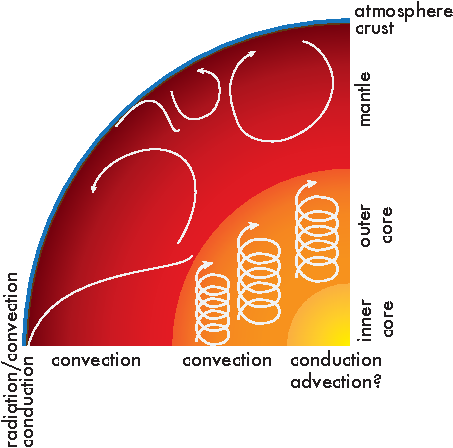
\includegraphics[]{geothermics/figures/earth_heat_mechanisms.pdf}
    \caption{Dominant mechanisms of heat transfer within the Earth.}
    \label{fig:hfmech}
\end{figure}

\subsection{Conduction}
Conduction is the dominant mode of heat transfer in most solid Earth settings relevant to geothermics. It arises from microscopic energy transport by lattice vibrations (phonon--phonon) and, to a lesser extent, free electrons.  Conduction operates in solids and stationary fluids and is the process that underpins essentially all steady-state geotherms and most transient thermal models in the crust and lithosphere.

In this chapter, conduction provides the primary physical link between temperature gradients and observable quantities such as surface heat flow. The diffusion of heat implied by Fourier's law introduces spatial smoothing and finite thermal memory, distinguishing geothermics from purely static potential-field methods.

\subsection{Advection (Convection)}
Advection refers to the transport of heat by the bulk motion of material. In the Earth, this includes mantle convection, magma migration, hydrothermal circulation, tectonic deformation and fluid flow in porous media. While advection can dominate heat transport in many geological environments, it is not treated explicitly as a governing process in many lithospheric thermal studies.

Instead, advective effects are commonly incorporated implicitly through:
\begin{itemize}
    \item boundary conditions---specifically transfer from the convecting mantle to the lithosphere,
    \item effective thermal properties, or
    \item source terms in the energy equation.
\end{itemize}
This approach reflects the focus of geothermics on thermal structure rather than fluid or solid mechanics. Where advection is dominant and explicitly time-dependent, the problem typically shifts into the domain of geodynamics or hydrogeology rather than classical geothermics.

\subsection{Radiation}
Radiative heat transfer involves the emission and absorption of electromagnetic radiation (photons) and governed by the Stefan--Boltzmann law. In the context of the solid Earth, radiative transfer is negligible except at very high temperatures (e.g., in the deep mantle) or at planetary surfaces. Consequently, radiation is not considered further in this chapter.


\section{Conservation of Energy}

The governing equations of geothermics follow directly from the conservation of energy. Consider a representative volume of material in which heat may be conducted ($\vb{q_c}$), advected by material motion ($\vb{q_a}$), radiated ($\vb{q_r}$) or internal sources or sinks ($\vb{q_p}$).  Thus the total vector heat flux out across the surface of a volume, $\vb{q}$, is given by the sum of each mode of transport, i.e.,
\begin{equation}
    \vb{q} = \vb{q_c} + \vb{q_a} + \vb{q_r} + \vb{q_p}.
\end{equation}
The radiative heat flux is generally small at crustal temperatures, but becomes significant at high temperature ($>$\SI{500}{^\circ C}). Often when it is included, it is treated as an enhanced conductive term so requires no special consideration.

In geophysical applications, conduction is described by Fourier's law, a constitutive relation between the conductive heat flux and the temperature gradient:
\begin{equation}
    \coreeq
    \vb{q_c} = k \, \grad{T},
    \label{eq:fourier}
\end{equation}
where $k$ is the thermal conductivity, and $T$ is temperature.
\ntextbox{Sign Convention}{
    Because the Earth is losing heat, the heat flow is up away from the surface of the Earth.  By the geophysical definition, this rate of heat loss (heat flow) is defined as positive.  In physics and engineering, the rate of heat loss is typically defined as negative (i.e.\ $q = - k \grad T$).
}{alert}
Advection results in additional heat flux by the direct transport of mass,
\begin{equation}
    \workeq
    \vb{q_a} = \rho C_P T \vb{u} ,
    \label{eq:advection}
\end{equation}
where $\rho$ is mass density, $C_P$ is specific heat capacity at constant pressure, $\vb{u}$ is the material or fluid velocity, and $T$ is temperature. We will often see coupled $\rho C_P$ in geothermics which is collectively known as the heat storage capacity or simply heat capacity.

In Earth, there are a number of potential sources and sinks of heat.  The most important and continuous source is due to radioactive decay.  Shear heating from deformation in shear zones, bending and folding, and slipping on faults all produces frictional heat.  This heating while important locally can add to regional heat flow over geologic time (Box~\ref{box:shearheat}).  Phase changes during melting and metamorphism can act as both a source (crystallization/retrograde) or sink (melting/prograde) of heat.  Although they can be written as an effective source term in the energy equation, their magnitude is controlled by the rate of reaction progress along a $P$--$T$ path, making them time dependent and fundamentally different from volumetric heat sources such as radiogenic and shear heating.  Melting and metamorphism are discussed further in Section~\ref{sec:stefan}.  Since radioactive heat generation dominates, we'll focus on this component of the internal heat flux, which is expressed as
\begin{equation}
    \workeq
    \vb{q_p} = A \vb{x}
    \label{eq:qsources}
\end{equation}
where $A$ is the heat production per unit volume.

\ntextbox{Shear heating in the Earth}{
    Deformation of a viscous material converts mechanical work into heat, a process known as \emph{shear heating} (or viscous dissipation).  In its most general form, the volumetric heating rate depends on the stress and the full velocity gradient.  However, for most geophysical applications, this expression can be simplified by working in terms of a characteristic strain rate.

    For a viscous material with effective viscosity $\eta$ and second invariant of the strain rate tensor $\dot{\varepsilon}$, the shear heating rate can be approximated as
    \[
        \Phi \approx \eta\,\dot{\varepsilon}^2,
    \]
    where $\Phi$ has units of \si{W.m^{-3}}.  This expression highlights two important features. First, shear heating is always positive, representing irreversible conversion of mechanical energy into heat.  Second, the heating rate scales with the square of the strain rate, so even modest increases in deformation rate can lead to large increases in heating.

    To assess the importance of shear heating, we can compare it with typical radiogenic heat production in the mantle, which is approximately $2 \times 10^{-8}~\si{W.m^{-3}}$

    Using representative mantle values ($\eta \sim 10^{21}$~\si{Pa.s}, $\dot{\varepsilon} \sim 10^{-15}~\si{s^{-1}}$), we find $\Phi \approx 10^{-9}~\si{W.m^{-3}}$.  This result is only a few percent of the radiogenic contribution.  Thus, in the convecting mantle interior, shear heating is typically negligible.  However, because $\Phi \propto \dot{\varepsilon}^2$, shear heating increases rapidly in regions where deformation is localized.  In lithospheric shear zones or subduction interfaces, strain rates can be orders of magnitude higher, and shear heating may become comparable to or exceed radiogenic heating.

    Strain rates in tectonic environments span many orders of magnitude (Table~\ref{tab:strainrates}), primarily reflecting differences in the spatial scale over which deformation occurs.
    \begin{center}
    \textbf{Table~\thetable:} Typical strain rates in tectonic settings and their implications for shear heating.
    \label{tab:strainrates}
    \begin{tabular}{lccc}
    \toprule
    \textbf{Setting} &
    \textbf{Strain rate}  &
    \textbf{Shear heat production} &
    \textbf{Importance} \\
    & (\si{s^{-1}}) & \si{W.m^{-3}} \\
    \midrule
    Mantle interior & $10^{-16}$--$10^{-15}$ & $10^{-11}$--$10^{-9}$ & negligible \\
    Mid-ocean ridges & $10^{-15}$--$10^{-14}$ & $10^{-9}$--$10^{-7}$ & small \\
    Subduction zones & $10^{-14}$--$10^{-13}$ & $10^{-7}$--$10^{-5}$ & moderate \\
    Lithospheric shear zones & $10^{-13}$--$10^{-12}$ & $10^{-5}$--$10^{-3}$ & important \\
    Earthquakes & $10^{-6}$--$10^{2}$ & $10^{1}$--$10^{9}$ and higher & extreme (transient) \\
    \bottomrule
    \end{tabular}
\end{center}

    Although shear heating is typically small in the well-mixed mantle interior, it can play an important role in localized regions of high strain.  In such settings, the strong dependence on strain rate can lead to thermal weakening, potentially promoting further localization of deformation.  This feedback is thought to be important in the development of plate boundaries and ductile shear zones.

    In tectonic environments, deformation is commonly concentrated into narrow zones such as faults and shear zones, so that high strain rates—and therefore significant shear heating—are restricted to relatively small volumes of the lithosphere.  As a result, while temperatures within these zones may locally increase substantially, in some cases even approaching melting conditions, the integrated effect on the thermal structure of the lithosphere as a whole is much smaller.

    In the crust, the presence of fluids along faults can further moderate the thermal impact of shear heating.  Fluid circulation enhances heat transport away from deforming zones, allowing heat to be dissipated more efficiently and reducing the magnitude and duration of local temperature increases.
}{aside}\label{box:shearheat}

Conservation of energy requires that the rate of change of internal energy equal the divergence of heat flux plus any internal heat sources.  In differential form, the general statement relevant to geothermics can be written as
\begin{equation}
    \pdv{(\rho C_P T)}{t} = \div{\vb{q}}.
\end{equation}
Writing energy conservation with the storage term form makes it explicit that density and heat capacity may vary with temperature.  Substituting Equations~\ref{eq:fourier}, \ref{eq:advection} and~\ref{eq:qsources} into the above, yields the advection--diffusion equation for heat:
\begin{equation}
    \coreeq
    \mlbox[
        labelstyle={xshift=-3em,yshift=-7em},
        linestyle={out=90,in=270, latex-}]
    {\pdv{(\rho C_P T)}{t}}{transient} =
    \mlbox[
        labelstyle={xshift=-3em,yshift=1em},
        linestyle={out=270,in=90, latex-}]
    {\div (k \grad T)}{diffusion} - 
    \mlbox[
        labelstyle={xshift=-3em,yshift=1em},
        linestyle={out=270,in=90, latex-}]
    {\div (\rho C_P \vb{u} T)}{advection} + 
    \mlbox[
        labelstyle={xshift=3em,yshift=-6em},
        linestyle={out=90,in=270, latex-}]
    {A}{sources},
  \label{eq:heateq}
\end{equation}
This equation is parabolic in time and describes the combined effects of thermal storage, diffusion, advective transport, and internal heat production. It forms the fundamental basis for both steady-state and transient thermal models, with different terms dominating in different geological environments.

In this text, we will generally ignore situations involving advection.  We will make additional simplifying assumptions to solve special cases consistent with tectonic scenarios.

\subsection{Steady-State and Conductive Limit}
In the absence of advection ($\vb{u}=0$) and when thermal conditions ($\pdv{T}{t} \approx 0$) do not change appreciably with time, the conservation-of-energy equation reduces to
\begin{equation}
    \coreeq
    \div (k \, \grad{T}) = -A.
\end{equation}
This elliptic equation governs steady-state conductive geotherms and places geothermics on the same mathematical footing as gravity, magnetics, and electrostatics, while retaining explicit dependence on material properties and internal heat sources.  This equation shows that the curvature of the temperature field is controlled directly by internal heat production and spatial variations in thermal conductivity.

\subsection{Interpretation}
The conservation-of-energy framework highlights three central features of geothermics:
\begin{enumerate}
    \item temperature is a state variable with finite storage capacity ($\rho C_P$),
    \item thermal structure reflects both present-day boundary conditions and the integrated effects of past processes, and
    \item departures from purely conductive behavior arise through advection and property variations rather than changes in the governing physical principle.
\end{enumerate}
These properties distinguish geothermics from static potential-field methods and motivate the explicit consideration of timescales, transients, material properties, and thermal memory throughout this chapter.

\ntextbox{The heat equation as a configurable system}{
    The heat equation (Equation~\ref{eq:heateq}) can be thought of as a configurable system, much like purchasing a car.

    At its simplest, one can choose the base model: no options, no add-ons, and no complexity. In geothermics, this corresponds to Laplace's equation, where there are no internal heat sources, no time dependence, and nothing moving (hopefully the base car moves). The problem is elegant, tractable, and often admits analytic solutions.

    Adding internal heat production is like selecting an upgraded engine. The governing equation becomes Poisson's equation, and while the physics becomes more realistic, the solution space becomes more complex. Curvature appears, and interpretation requires additional information.

    Including time dependence introduces another major upgrade. The full diffusion equation describes how temperature evolves, retains memory of past conditions, and responds on characteristic timescales set by thermal diffusivity. Many previously simple problems now require numerical solutions.

    Additional features—such as advection, latent heat, moving boundaries, or variable material properties—each add capability but also cost. The governing equation remains the same in principle, but solutions become progressively harder to obtain and harder to interpret.

    Just as with a car, the question is not whether one should always choose the most fully equipped option, but which configuration is appropriate for the problem at hand.
}{aside}


\section{Thermal Properties of Earth Materials}
This is where geothermics really differentiates itself from gravity and magnetics.

This section develops the thermal properties that control conductive and transient heat transport in the lithosphere, with emphasis on thermal conductivity and radiogenic heat production. The goal is not to present canonical constants, but to show how these properties vary systematically with lithology, composition, temperature, pressure, metamorphic grade, and tectonic setting, and how those variations influence geothermics and interpretation. Rather than treating thermal properties as fixed parameters, they are presented here as spatially variable fields whose structure reflects geological history.

The treatment leans on recent syntheses and global compilations, particularly for continental crustal rocks, which have substantially revised earlier assumptions about uniformity and simple depth dependence of thermal properties.


\subsection{Thermal Conductivity, $k$}
\subsubsection{Functional Role of Conductivity}
Thermal conductivity, $k$, controls how efficiently heat is redistributed by conduction and therefore governs both the shape of geotherms and the attenuation of lateral thermal variations. In most crustal rocks, heat is transported primarily by lattice vibrations (phonons), with a smaller contribution from free electrons that becomes significant only in metallic or graphitic materials. The efficiency of this transport is reduced by scattering from defects, grain boundaries, and interfaces between mineral phases, so that conductivity depends sensitively on mineralogy, microstructure, and fabric.

A central point for geothermics is that thermal conductivity redistributes heat but does not generate it. As a result, conductivity primarily controls temperature gradients and the smoothing of thermal structure, rather than the absolute thermal budget. Variations in $k$ therefore influence how heat is expressed spatially, not how much heat is available.

Thermal conductivity is not constant, even within a single lithology. In crystalline rocks it generally decreases with increasing temperature, reflecting enhanced phonon scattering at higher vibrational energies. Pressure effects are typically weaker but become non-negligible at lower crustal conditions. Together, these dependencies introduce nonlinearity into both steady-state and transient thermal models when large temperature ranges are involved, and motivate the use of temperature-dependent conductivity in lithospheric studies rather than constant values. Recent work has emphasized that neglecting this dependence can lead to systematic biases in inferred geotherms, particularly in the lower crust and lithosphere.

In many geological settings, thermal conductivity is anisotropic. Foliation, layering, and mineral alignment can cause heat to flow more readily in some directions than others. Even when anisotropy is modest, spatial variations in $k$ lead to thermal refraction, in which heat flow is redirected across lithological boundaries. This effect is directly analogous to refraction in other potential fields and can significantly alter local geothermal gradients without changing the total heat flux.

\subsubsection{Compositional Variations}

Conductivity varies systematically with lithology and composition. These differences matter in geothermics not because they change how much heat is generated, but because they control how efficiently heat is redistributed through the crust.  Felsic rocks tend to exhibit lower conductivities than mafic rocks (Figure~\ref{fig:tc_rock_type}), while quartz content exerts a first-order control in many common crustal lithologies. Metamorphic recrystallization can further modify conductivity through grain growth, phase changes, and the destruction or enhancement of preferred mineral alignments. Global datasets demonstrate that these lithology-dependent variations are large enough to matter for regional and continental-scale geotherms, especially in the upper crust where lateral heterogeneity is greatest.
\begin{figure}
    \centering
    
\includegraphics[width=14cm]{geothermics/figures/conductivity_distributions.pdf}
    \caption{Thermal conductivity of common igneous and metaigneous and a few metasedimentary rock types.  Rock types have been recomputed based on chemistry for consistent naming.  The rock types are ordered vertically with \ce{SiO2} from highest at the top to lowest at the bottom.}
    \label{fig:tc_rock_type}
\end{figure}


Unlike heat production, which can be highly variable for any given rock type, thermal conductivity is easier to estimate.  A number of mixing laws have been used to estimate thermal conductivity either of a rock with varying porosity, or as an assemblage of minerals.  The most common mixing relation used to estimate the effective thermal conductivity is the geometric mean:
\begin{equation}
    k_{\mathrm{eff}} = \prod_{i=1}^{N} k_{i}^{\chi_{i}},\;
    i = 1, 2, \ldots N,
\end{equation}
where $\chi_{i}$ is the volume fraction of the constituent minerals and/or pore filling components.  Note: the notation denoted by,$\prod$, indicates a product analogous to $\sum$, e.g., $\prod_{i=1}^N a_i^2 = a_1^2 a_2^2 a_3^2 \cdots a_N^2$. The geometric mean as a mixing model works best for rocks where the minerals are randomly arranged and oriented and so works best for fresh igneous rocks. The thermal conductivity of several common minerals are listed in Table~\ref{tab:tcmin}.
\begin{table}[bpht]
    \centering
    \begin{threeparttable}
    \caption{Thermal conductivity of common materials.}
    \label{tab:tcmin}
    \begin{tabular}{lc}
        \toprule
        {} &
        $k$ \\
        mineral &
        W m$^{-1}$K$^{-1}$ \\
        \midrule
        air               & 0.026  \\
        water             & 0.6    \\
        ice               & 2.5 (@ -30\degC) \\
        oil               & 0.13   \\
        salt (halite, sylvite) & 6, 7 \\
        iron              & 80 \\
        copper            & 401 \\
        calcite           & 3.6   \\
        $\alpha$-quartz   & 8.8   \\
        orthoclase        & 1.8   \\
        plagioclase, felsic (Ab$_{80}$An$_{20}$) & 1.8 \\
        plagioclase, mafic (Ab$_{35}$An$_{65}$) & 1.6 \\
        mica, muscovite ($\parallel$,$\perp$)   &  3.9, 0.6  \\
        mica, biotite ($\parallel$,$\perp$)     &  3.1, 0.5  \\
        hornblende        &  2.7  \\
        clinopyroxene (Di$_{90}$Hd$_{10}$)    &  4.3  \\
        orthopyroxene (En$_{90}$Fs$_{10}$)     &  3.4  \\
        olivine (Fo$_{90}$) &  4.8  \\
        spinel (Sp$_{75}$Mt$_{25}$) & 9? \\
        garnet (Py$_{70}$Al$_{30}$)       &  3.9 \\
        \bottomrule
    \end{tabular}
    \begin{tablenotes}
        \item All conductivities estimated at \SI{25}{\degC}.
    \end{tablenotes}
    \end{threeparttable}
\end{table}
 % tab:tcmin

For silicate rocks and clastic sediments, the dominant control on the thermal conductivity is the quartz content as it has a thermal conductivity significantly higher than most other common minerals.  For sedimentary rocks the porosity is also very important.

Like most physical properties of rocks, thermal conductivity is sensitive to pressure and temperature effects.  Thermal conductivity typically decreases with temperature while pressure tends to slightly increase the thermal conductivity slightly.  The thermal conductivity of most rocks tend to about \SI{2.5}{\tcu}\ at high temperatures regardless of their mineralogy.  An example is shown for olivine in Figure~\ref{fig-kol}.
\begin{figure}[hbtp]
  \centering
  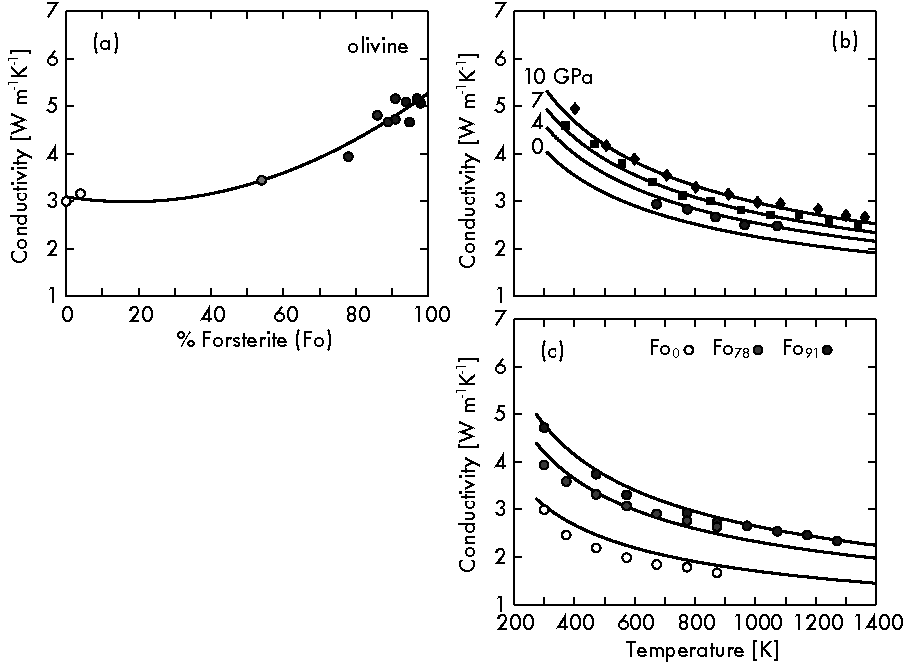
\includegraphics{geothermics/figures/k_olivine.pdf}
  \caption{Thermal conductivity of olivine. (a) Compositional dependence at
  \SI{298}{K}. (b) Pressure and temperature dependence. (c) Compositional and
  temperature dependence.}
  \label{fig-kol}
\end{figure}

At higher temperatures, generally $>\SI{500}{\degC}$, thermal conductivity is enhanced by radiative transmission.  At high temperatures, some minerals are transparent, allowing photons to transfer energy at a greater distance through the crystal until they interact with the lattice (photon-phonon transmission).  However, the radiative effect for many minerals is still poorly constrained. Recent experiments on olivine suggest the influence is nearly double what was previously believed \citep{Marzotto_etal2025}.

\subsection{Anisotropy}
Thermal conductivity is an anisotropic property, meaning that its magnitude depends on the orientation along which it is measured.  Anisotropy can arise at micro-, meso-, and macroscopic scales.  Macroscopic anisotropy, discussed further in Section~\ref{sec:thermresist}, reflects large-scale heterogeneities such as stratified lithologies or laterally continuous compositional layers.  Mesoscopic anisotropy operates at the scale of hand samples or outcrops and is the focus of this section.

Mesoscopic anisotropy may result from compositional layering, preferred orientation of intrinsically anisotropic minerals, or a combination of both.  At this scale, anisotropy commonly develops during deformation, where shearing and compaction produce foliation or lineation that aligns mineral grains and pores.  This alignment creates a plane of approximately uniform thermal conductivity, with a perpendicular direction that exhibits a distinct value.

Many common rock-forming minerals exhibit crystallographic anisotropy in thermal conductivity, including quartz, feldspar, pyroxene, and olivine.  In contrast, garnet is one of the few major rock-forming minerals that is effectively isotropic due to its isometric crystal structure.  Consequently, bulk-rock anisotropy is strongly controlled by both mineral assemblage and fabric, rather than by composition alone.

Anisotropy is typically quantified by measuring thermal conductivity along multiple orientations relative to foliation or lineation (Figure~\ref{fig:tc_anisotropy}).  For samples with transverse isotropy, an anisotropy factor can be defined as
\[
    \workeq
    \Lambda = \frac{\max(k_\parallel,k_\perp)}{\min(k_\parallel,k_\perp)},
\]
where $k_\parallel$ and $k_\perp$ denote conductivities measured parallel and perpendicular to the foliation plane, respectively.
\begin{figure}[tbh]
    \centering
    
\includegraphics[]{physprop/figures/observed_anisotropy_angle.eps}
    \caption{Directional dependence of thermal conductivity measured relative to fabric orientation in an anisotropic metasedimentary samples. Conductivity measured parallel to layering or mineral alignment differs systematically from measurements made perpendicular to layering.}
    \label{fig:tc_anisotropy}
\end{figure}

Among sedimentary and metasedimentary rocks, both isotropic and anisotropic behaviors are observed.  Anisotropy cannot be predicted uniquely from bulk composition alone, as it depends on the degree of fabric development and mineral alignment.  However, certain compositions are more prone to anisotropy than others.  In particular, rocks with bulk compositions near \SI{65}{wt\%} \ce{SiO2} commonly exhibit elevated anisotropy factors (Figure~\ref{fig:k_aniso}), coinciding with peak abundances of sheet silicates.  These minerals possess strong intrinsic anisotropy and readily align during deformation, amplifying bulk thermal conductivity contrasts.
\begin{figure}[hbtp]
    \centering
    \includegraphics[]{geothermics/figures/k_anisotropy_oxides.eps}
    \caption{Anisotropy factor variations with \ce{SiO2} and \ce{K2O}.  While there is not a single function to describe the data, the envelope of permissible anisotropy factors varies with composition.}
    \label{fig:k_aniso}
\end{figure}
%- Lithology variations
% Add a figure like the heat production for thermal conductivity
%- Anisotropy
% Add a figure with thermal conductivity anisotropy and SiO2, repeat of figure from the physical properties chapter.

\subsection{Radiogenic Heat Production, $A$}

\section{Heat Production, $A$}

Radiogenic heat production, $A$, supplies internal energy to the crust and is the primary control on the curvature of continental geotherms. In contrast to thermal conductivity, which redistributes heat without creating or destroying energy, heat production acts as a true volumetric source term in the heat equation. As a result, it governs how temperature departs from linearity with depth and exerts first-order control on crustal thermal structure.

At present day, crustal heat production is overwhelmingly dominated by the radioactive decay of potassium, thorium, and uranium, which together account for $\gtrapprox 99\%$ of radiogenic heat generation. Minor contributions arise from rubidium and samarium  (Table~\ref{tab:radiostopes}). Numerous other naturally occurring radioisotopes exist, but their present-day contribution to Earth''s heat budget is negligible.

Heat production is not constant through geological time because radioactive decay reduces the abundance of key isotopes (Box~\ref{box:hp_time}). This process is monotonically decreasing with age. Reconstructing past geotherms therefore requires accounting for the time evolution of isotope abundances and the resulting change in heat production.
\begin{table}
    \centering
    \begin{threeparttable}
    \caption{A table of radiogenic isotopes relevant to Earth's heat production \citep{McDonough_etal2020}.}
    \label{tab:radisotopes}
    \begin{tabular}{@{}ccccc@{}}
        \toprule
        \textbf{Isotope} &
        \textbf{Half-life} &
        \textbf{Decay Constant} &
        \textbf{Abundance}\tnote{a} &
        \textbf{Heat Generation} \\
        & \si{Ma} & \si{a^{-1}} & \% & \si{\mu W.kg^{-1}} \\
        \midrule
        \ce{^{26}Al}  & \SI{0.717(24)}{ka} & $9.67 \times 10^{-7}$    & 0        & $3.41 \times 10^5$ \\
        \ce{^{40}K}   & $1.262(2)$    & $5.491 \times 10^{-10}$  & $1.167 \times 10^{-4}$ & 29.029 \\
        \ce{^{60}Fe}  & \SI{2.62(4)}{ka}  & $2.65 \times 10^{-7}$    & 0        & $3.99 \times 10^4$ \\
        \ce{^{87}Rb}  & $49.61(16)$   & $1.397 \times 10^{-11}$  & 0.2783   & 0.04082 \\
        \ce{^{147}Sm} & $106.3(5)$    & $6.539 \times 10^{-12}$  & 0.14993  & 0.3073 \\
        \ce{^{232}Th} & $14.1(1)$     & $4.92 \times 10^{-11}$   & 1.0000   & 26.180 \\
        \ce{^{235}U}  & $0.70348(20)$ & $9.8531 \times 10^{-10}$ & 31.223   & 561.65 \\
        \ce{^{238}U}  & $4.4683(96)$  & $1.5513 \times 10^{-10}$ & 0.992740 & 94.936 \\
        \bottomrule
        \addlinespace[0.6em]
    \end{tabular}
    \begin{tablenotes}
        \item[a]Short lived isotopes \ce{^{26}Al} and \ce{^{60}Fe} are negligible today, but would have been important contributors to the heat production in the early Earth.
    \end{tablenotes}
    \end{threeparttable}
\end{table}

If we go back in time to the formation of Earth, two short-lived radionuclides---\ce{^{26}Al} and \ce{^{60}Fe}---played a major role during Earth's earliest evolution. During the first $\lesssim$20~Ma of planetary history, decay of these isotopes generated nearly \SI{1000}{TW} of heat, profoundly influencing early melting and differentiation. Although their abundances are now negligible, some of this early thermal energy continues to be lost from Earth's interior. By comparison, radiogenic heat production today is approximately \SI{20}{TW}. Relevant radiogenic isotopes and their properties are summarized in Table~\ref{tab:radisotopes}.

\subsection{Quantifying Heat Production}

Present-day heat production can be computed directly from bulk chemical compositions using
\begin{equation}
    \workeq
    A~[\hgu] = \rho \left(3.387 \times 10^{-3}\,\ce{K} + 26.18\,\ce{Th} + 98.29\,\ce{U} + 0.01139\,\ce{Rb} + 0.04595\,\ce{Sm}\right),
\end{equation}
where elemental concentrations are given in weight percent and $\rho$ is density. Because uranium and thorium have much higher heat productivity per unit mass than potassium, small variations in trace-element abundance can dominate $A$ even when K varies substantially.

Heat-producing elements are not uniformly distributed among rock-forming minerals. Instead, they are preferentially concentrated in accessory phases such as zircon, monazite, xenotime, allanite, apatite, and related phosphates. Consequently, radiogenic heat production is highly sensitive to magmatic differentiation, partial melting, sedimentary recycling, and other crustal processing mechanisms. This leads to variations in $A$ spanning several orders of magnitude among lithologies (Figure~\ref{fig:hp_rtype}), even within a single tectonic province.
\begin{figure}[htp]
    \centering
    \includegraphics[]{geothermics/figures/hp_rtype.eps}
    \caption{Heat production of (a) plutonic (igneous) and (b) sedimentary rock types determined from a global geochemical database \citep{Hasterok_etal2017}.  Inset diagrams display the chemical divisions used to define the igneous and sedimentary rock types, respectively.}
\end{figure}

\subsection{Geological Controls on Heat Production}

Potassium behaves as a major element and is abundant in feldspars, micas, clays, and some amphiboles, all common constituents of the upper crust. Uranium and thorium, by contrast, are trace elements and are typically hosted in dense accessory minerals, particularly monazite-group phosphates. These minerals may be mechanically concentrated during weathering and sedimentary sorting, allowing heat-producing elements to become enriched in specific depositional environments (Figure~\ref{fig:hpe}).

All major heat-producing elements are incompatible during partial melting. Melting therefore preferentially extracts K, Th, and U from the source rock and transports them toward the surface, where they are further concentrated by fractional crystallization or sedimentary reworking (Figure~\ref{fig:hpe}). In addition, uranium is mobile in oxidizing fluids and may be redistributed by groundwater, leading to enrichment in mudstones, shales, and other fine-grained sedimentary rocks.
\begin{figure}[htbp]
    \centering
    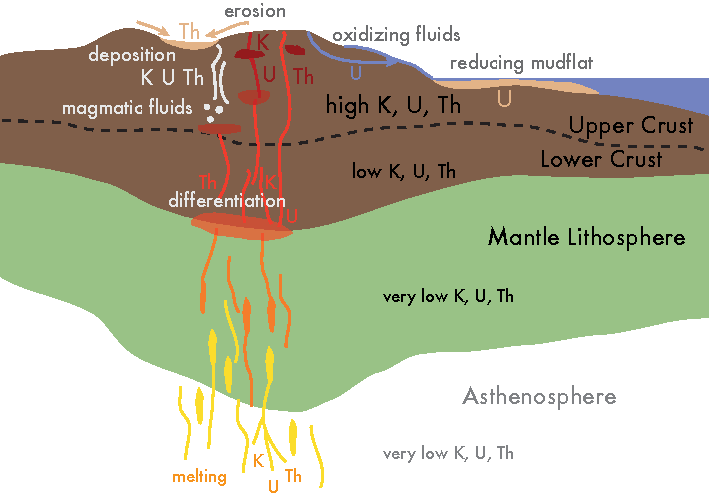
\includegraphics[]{geothermics/figures/hpe_dynamics.pdf}
    \caption{Dynamics of heat producing elements and their path from the mantle
    to concentrations within the crust.}
    \label{fig:hpe}
\end{figure}

Systematic differences in heat production are observed across tectonic settings. Felsic and intermediate compositions generally exhibit higher heat production than mafic rocks, while cratons, mobile belts, arcs, and sedimentary basins occupy distinct characteristic ranges.

There is a prevailing view that metamorphic grade and repeated crustal reworking can further redistribute heat-producing elements, modifying thermal structure over time.  Early studies of heat production were interpreted as a decreasing heat production with increasing metamorphic grade. The datasets that these were based on were small, not based on individual lithologies, and produced mixed results.  More recent studies, including several high-resolution surveys by \citet{Alessio_etal2018} suggest that heat production is not affected.  More work is needed, but be careful accepting old wisdom before you know where it comes from.

Heat production varies with igneous crystallization age. For much of the past \SI{2.0}{Ga}, heat production in igneous rocks occupies a relatively narrow range, while older crust shows a systematic decrease in $A$ with increasing age (Figure~\ref{fig:hp_age}). Because mid-ocean ridge basalts derive from strongly depleted mantle sources, their heat production is substantially lower than that of continental lithosphere. Typical values for major lithospheric reservoirs are summarized in Table~\ref{tab:hpe}.
\begin{figure}[hbtp]
    \centering
    \includegraphics[]{geothermics/figures/hp_v_age.eps}
    \caption{Heat production variations with age for several igneous rock compositions \citep{Gard_etal2019a}.}
    \label{fig:hp_age}
\end{figure}
\begin{table}[hbtp]
    \centering
    \caption{Heat production averages.}
    \label{tab:hpe}
    \begin{tabular}{lc}
        \toprule
        {} & \textbf{Heat Production} \\
        \textbf{Reservoir} & \hgu \\
        \midrule
        \multicolumn{2}{c}{\it continental} \\
        upper crust &   2 \\
        lower crust &   0.4 \\
        mantle lithosphere &    0.02 \\
        \multicolumn{2}{c}{\it oceanic} \\
        crust, altered (unaltered) & 0.07 (0.3) \\
        mantle lithosphere & 0.002 \\
        \bottomrule
    \end{tabular}
\end{table}

Recent studies reveal systematic relationships between radiogenic heat production, magmatic differentiation, and crustal thickness in arc systems (Figure~\ref{fig:hp_arcs}). Although the underlying mechanisms are not yet fully understood, similar trends are observed for many trace elements, suggesting that heat production is part of a broader geochemical signal associated with crustal growth. These relationships link geothermics with petrology and tectonics, highlighting thermal properties as valuable tracers of crustal evolution.
\begin{figure}[htbp]
    \centering
    \includegraphics[]{geothermics/figures/hp_v_moho.eps}
    \caption{Heat production in recent arc volcanics and their relationship to crustal thickness.  The three arcs circled in grey are excluded from the analysis as their heat production is anomalous, likely resulting from the recent subduction of continental crust and/or thick continental derived sediments (\emph{Hasterok unpublished}).}
    \label{fig:hp_arcs}
\end{figure}

Two key conclusions follow. First, heat production is generally highest in the upper crust, lower in the lower crust, and lowest in the mantle. Second, the natural variability of heat production is sufficiently large that reliable estimates require direct observation---either geochemical analysis or gamma-ray spectrometry---rather than inference alone.

\subsection{Depth Distributions and Modeling Assumptions}

Constraints on how heat production varies with depth in the crust remain incomplete and, in some cases, contradictory. From a thermal modeling perspective, one requirement is clear: if surface-measured heat production is extended to excessive depths, conductive geotherms fail to intersect the mantle adiabat. This fundamental constraint implies that heat production must decrease downward on average, but it does not uniquely determine how that decrease is achieved.

Geological and geophysical observations provide competing lines of evidence. Seismic velocity models and bulk chemical arguments suggest that the crust becomes progressively more mafic with depth, which would imply a systematic reduction in heat production due to lithologic control. However, even when surface heat production values appropriate for mafic compositions are extended downward, model geotherms commonly remain too warm. Direct observations from lower-crustal xenoliths are broadly consistent with reduced heat production, but these samples are drawn from a limited number of terranes and may be biased toward Archean crust, which is itself characterized by relatively low heat production.

At the same time, some recent models of crustal composition argue that the lower crust may be more felsic than traditionally assumed. Granulite-facies felsic rocks can exhibit densities and seismic velocities comparable to those of lower-crustal mafic rocks, complicating purely seismic interpretations. If such compositions are widespread, they would imply higher heat production at depth than standard mafic models suggest. Nevertheless, surface heat production observations still require that average lower-crustal values be lower than those inferred from exposed upper-crustal rocks, even if the precise magnitude and cause of the decrease remain uncertain.

To represent this downward reduction in heat production, many thermal models adopt an exponential decay of heat production with depth. This parameterization is computationally convenient but lacks a physical basis, and should not be interpreted as a process-based description. Global geochemical compilations reveal large variability in heat production among terranes of similar thickness and structure, indicating that depth distributions are not governed by simple physical rules. Instead, they emerge from the cumulative effects of magmatism, sedimentation, metamorphism, and tectonic accretion through time.

These observations emphasize that heat production is geologically structured rather than smoothly varying with depth. Its distribution reflects crustal assembly history as much as present-day lithology. As a consequence, assumptions about $A(z)$ represent one of the dominant sources of uncertainty in crustal geotherm modeling, and simple parameterizations should be treated as pragmatic approximations rather than physically meaningful descriptions.

\subsection{Modeling Consequences}

Thermal conductivity and heat production jointly determine the shape of geotherms. Heat production primarily controls curvature, while conductivity governs the magnitude of temperature gradients (temperature--depth slope) and the redistribution of heat. Because different combinations of $k$ and $A$ can yield similar temperature-depth profiles, trade-offs between these parameters are a major source of non-uniqueness in thermal models. Robust interpretation therefore requires independent geological or geophysical constraints on both properties.

Several general implications follow for geothermics. Thermal properties should be treated as spatially variable fields rather than fixed constants, particularly in the upper crust where lateral heterogeneity is pronounced. Variations in conductivity and heat production can produce substantial differences in local geotherms even when surface heat flow is similar. Simple parameterizations may reproduce average behavior but often fail to capture observed variability, underscoring the importance of geological constraints, temperature-dependent properties, and sensitivity analysis in both steady-state and transient models.

\ntextbox{Time Dependence of Radiogenic Heat Production}{
    Radiogenic heat production decreases with time as radioactive isotopes decay. Reconstructing geotherms in the geological past therefore requires explicit accounting for the time evolution of isotope abundances and their heat production. The expressions below provide a framework for computing past heat production directly from present-day rock compositions and are intended for use in forward thermal modeling exercises.

    The heat production contribution from a single isotope, $i$, from element, $j$, is given by
    \[
        A_{i,j} = \rho H_{i,j} C_{i,j} ,
    \]
    where $\rho$ is the rock density, $H_i,j$ is the heat production per unit mass and $C_i,j$ is the mass fraction (\si{kg}/\si{kg}) of the isotope.  Since we typically measure the concentration of elements rather than isotopes in a rock, we can write the heat production contribution as
    \[
        A_{i,j} = \rho H_{i,j} X_{i,j} C_j
    \]
    where $X_{i,j}$ is the aboundance of isotope $i$ in element $j$.

    For the radioactive isotope, $X_{i,j}$, the number of atoms decreases exponentially with time.  Turning the equation around to solve for the heat produced in the past,
    \begin{equation}
        \workeq
        X_{i,j}(t) = X_{i,j,0}\,e^{\lambda_i t},
    \end{equation}
    where $\lambda_i$ is the decay constant for isotope $i$, and $t$ is time defined as positive moving into the geological past.

    The total volumetric heat production at time $t$ is then
    \[
        \workeq
        A(t) = \rho \sum_i \sum_j H_{i,j} X_{i,j,0} C_{j} \,e^{+\lambda_i t},
    \]
    with the summation taken over all heat-producing isotopes and $\rho$ the rock density. Note that this formulation assumes closed-system behavior and constant bulk composition through time.

    For practical applications involving crustal rocks younger than approximately \SI{4}{Ga}, the dominant contributions come from \ce{^{238}U}, \ce{^{235}U}, \ce{^{232}Th}, and \ce{^{40}K}. Because \ce{^{235}U} has a much shorter half-life than \ce{^{238}U}, the uranium contribution to ancient heat production increases disproportionately with age, resulting in substantially higher Archean heat production for otherwise identical bulk compositions.

    When coupled with steady-state or transient heat conduction models, these time-dependent heat production terms provide first-order estimates of geotherms throughout Earth history. Even modest increases in $A$ can significantly raise temperatures at depth, highlighting the sensitivity of continental geotherms to the temporal evolution of radiogenic heat sources.
}{core}\label{box:hp_time}

\section{Mantle adiabat and lithospheric thickness}

The conductive lithosphere does not extend indefinitely. Its base is defined by the transition to convecting mantle, whose temperature follows an adiabat (more precisely, an isentrope).

\subsection{Mantle adiabat}
In a convecting fluid with minimial conduction, there is little heat exchanged with the surroundings, resulting in an adiabatic processes (no heat loss). If the process is reversable then it is also isentropic (no entropy loss). The change in pressure during this process is accompanied by a change in temperature.  When temperatures are superadiabtic, material rises, and when they are subadiabatic, the material falls, resulting in convection.

To a reasonable approximation, this describes convection in Earth's mantle, with heat exchanged only at the thermal boundary layers (core--mantle and asthenosphere--lithosphere boundaries.).  It can be shown from the heat equation that this change in temperature with pressure is approximate by
\[
    \left(\frac{\partial T}{\partial P}\right)_S = \frac{\alpha T}{\rho C_P},
\]
where $\alpha$ is the coefficient of thermal expansion, $g$ is gravitational
acceleration, $T$ is temperature, and $C_P$ is the heat capacity at constant
pressure.  This expression can be converted to depth using $dP/dz = \rho g$, giving
\[
    \left(\dv{T}{z}\right)_S \approx \frac{\alpha g T}{C_P}.
\]
The adiabat when projected to the surface reaches what is know as the mantle potential temperature, $T_p$, resulting in a convecting mantle geotherm estimated as
\[
    T_m(z) \approx T_p + z\, \left( \dv{T}{z} \right)_S.
\]
Typical upper-mantle values yield gradients of order 0.3--\SI{0.5}{K.km^{-1}} (Box~\ref{box:adiabat}).

\ntextbox{Estimating the mantle adiabatic gradient}{
    Using the depth formulation for the adiabatic gradient, consider the representative thermophysical properties for fertile upper-mantle garnet lherzolite:
    \begin{align*}
        \alpha &\approx 3\times10^{-5}\,\mathrm{K^{-1}}, \\
        C_P &\approx 1.2\times10^{3}\,\mathrm{J\,kg^{-1}\,K^{-1}}, \\
        T &\approx 1623\,\mathrm{K}, \\
        g &= 9.8\,\mathrm{m\,s^{-2}}.
    \end{align*}

    Substituting these values gives
    \[
        \left( \dv{T}{z} \right)_S
        \approx
        \frac{(3\times10^{-5})(9.8)(1623)}{1.2\times10^{3}}
        \approx 3.9\times10^{-4}\,\mathrm{K\,m^{-1}}
        \approx 0.39\,\mathrm{K\,km^{-1}}.
    \]

    Over a depth interval of 100~km, the mantle adiabat therefore increases temperature by only $\sim 35$--$\SI{40}{K}$, which is small compared with typical conductive gradients in the lithosphere. This modest slope explains why the lithosphere--asthenosphere boundary is controlled primarily by the conductive geotherm rather than by rapid temperature increase in the convecting mantle.
}{mathtool}\label{box:adiabat}

\subsection{Lithospheric Thickness}

The lithosphere--asthenosphere boundary (LAB) is defined by the transition from a convecting mantle to a conducting lithosphere.  This intersection is defines the depth to the base of the lithosphere, $z = z_L$, i.e., 
\[
    T_{cond}(z_L) = T_m(z_L).
\]
In reality, the transition is not perfectly sharp. Rheological softening, partial melting, and small-scale convection smooth the boundary over tens of kilometers. Nevertheless, the intersection criterion provides a robust and interpretable thermal definition of the lithosphere that links surface observables to mantle conditions.  This thermal definition and may differ from the seismologically defined LAB, which takes a rheological view, though they are often similar in depth.


%----------------------------------------------------------
\section{Steady-State Geotherms}\label{sec:ss}

Steady-state conduction occurs as the long-term asymptotic stabilization of temperature following a transient process. Steady-state geotherms are most applicable to continental geotherms, particularly for those regions which have not experienced tectonic activity in the past few 10's of millions of years. One-dimensional states are sufficiently simple to model analytically, though 2- and 3-D geometries are often sufficiently challenging that they need to be modeled by numerical methods. In this section, we will explore several one-dimensional solutions that are still commonly employed.

\subsection{Homogeneous Lithosphere}

The heat equation as it is written in Equation~\ref{eq:heateq} is very complex; however, we reduce many of the complexities and still reasonably estimate temperatures within the Earth by making reasonable assumptions.
\begin{description}
  \item[Assumption 1:] $\pdv{T}{t} = 0$, i.e., steady-state conditions. \\ This assumption can be risky; however, the time constant for heat transport through a \SI{50}{km} thick lithosphere is approximately \SI{20}{My}.  Rifting in the Basin and Range began in earnest \SI{17}{Ma}, therefore, the lithosphere could be approximated by a near steady-state geotherm.  While this assumption works for many continental regions, it is a poor assumption for evolution of the oceanic lithosphere.

  \item[Assumption 2:] Lateral heat flow is negligible, i.e. $\pdv{T}{x}
  \approx \pdv{T}{y} \approx 0$. \\
  On a large scale, the temperature gradient vertically is approximately two orders of magnitude higher than the lateral gradients, thus the flow of heat is dominated by vertical heat transport.

  \item[Assumption 3:] No advection, i.e., $u = 0$. \\
  While magmatism does bring some heat to the surface, the quantity is too small to be significant for the large scale thermal structure, but can be very important locally (e.g., geothermal areas).

  \item[Assumption 4:] Constant thermophysical properties, e.g.,
  $\pdv{k}{P} = \pdv{k}{T} = 0$. \\
  This assumption is of course not true, but as you will see in Sections~\ref{sec:layeredT} we can work around this complexity by assuming that the properties are constant in sufficiently thin layers.
\end{description}

Making the above assumptions, the heat equation (Equation~\ref{eq:heateq}) is reduced to the differential governing 1-D steady-state heat conduction given by
\begin{equation}
    \dv[2]{T}{z} = -\frac{A}{k}.
    \label{eq-diff}
\end{equation}
To solve this differential equation we need two boundary conditions.  The simplest solution requires surface temperature and heat flow, $T_s$ and $q_{0}$, respectively.  These quantities are possible to measure or estimate relatively easily.  First, we integrate over depth,
\begin{align*}
  \int \dv[2]{T}{z} \dd{z} & = -\int \frac{A}{k} \dd{z}, \\
  \dv{T}{z} & = C_{0} - \frac{A}{k} z,
\end{align*}
giving us the constant $C_{0}$.  At $z = 0$, $\left. \dv{T}{z} \right|_{z=0} = C_{0}$; recalling Fourier's law, $\frac{q_{0}}{k} = C_{0}$.

Integrating a second time, we find:
\begin{align*}
    \int \dv{T}{z} \dd{z} & =
        \int \left( \frac{q_{0}}{k} - \frac{A}{k} z \right) \dd{z} \\
    T & = C_{1} + \frac{q_{0}}{k} z - \frac{A}{2 k} z^{2}.
\end{align*}
Applying the surface boundary condition, $T_{0} = C_{1}$, we arrive at the solution,
\begin{equation}
    \coreeq
    T(z) = T_{0} + \frac{q_{0}}{k} z - \frac{A}{2 k} z^{2}.
    \label{eq:ssgtherm}
\end{equation} 

\subsection{Layered Lithosphere}\label{sec:layeredT}

The homogeneous solution assumes that the thermophysical properties, $k$ and $A$, are constant.  However, thermal conductivity is sensitive to pressure, temperature, and rock type, and heat generation is sensitive to variations in the heat producing elements (U, Th, and K).  All is not lost.  If we make layers thin enough we can assume that the conductivity and heat production are constant with each layer (Figure
\ref{fig:layers}).
\begin{figure}[hbtp]
  \centering
  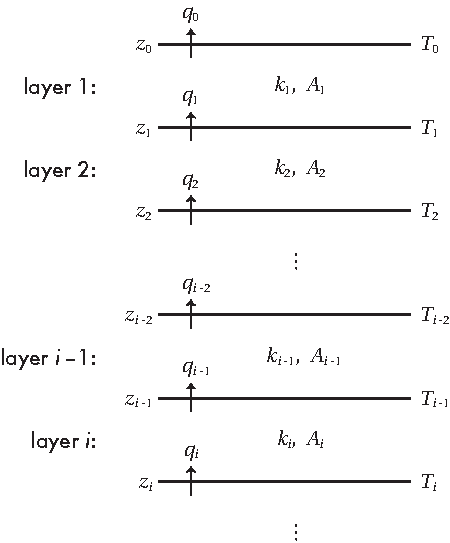
\includegraphics{geothermics/figures/thermal_layers.pdf}
  \caption{Model setup for 1-D steady-state conductive geotherms.}
  \label{fig:layers}
\end{figure}

The solution for the temperature at the base of the first layer, $T_1$, can then be estimated using the homogeneous solution,
\[
    T_1 = T_0 + \frac{q_0}{k_1} (z_1 - z_0) - \frac{A_1}{2 k_1} (z_1 - z_0)^2.
\]
The heat flow at the base of the first layer is equal to
\[
    q_1 = q_0 - A_1 (z_1 - z_0).
\]
The homogeneous solution can then be used to estimate the temperature at the base of the second layer using, $T_1$, as the temperature at the top and $q_1$ as the heat flow.  The temperature of all subsequent layers can be found using the same method boot-strapping down through the domain of interest.  

Solving for the temperature at the base of the $i$-th layer,
\begin{equation}
    \workeq
    T_{i} = T_{i-1} + \frac{q_{i-1}}{k_i} (z_i - z_{i-1})
    - \frac{A_i}{2 k_i} (z_i - z_{i-1})^2.
\end{equation}
It is also necessary to know the heat loss at the base of each layer in order to compute temperature.  Since heat flow is determined by the heat flowing into a layer plus the heat generated within, the heat flow at the bottom of each layer is given by
\begin{equation}
    \workeq
    q_i = q_{i-1} - A_i (z_i - z_{i-1}).
\end{equation}
This solution forms the basis of most 1-D steady-state geotherms.

\ntextbox{Classic Perspective on Geotherms}{
    There are a few classic ideas about how geotherms are constructed that are worth knowing even if their foundational principles are incorrect.  They stem from the historical development of our understanding about heat production and heat flow in the continental lithsphere starting in the 1960's.  The general trends advanced by these models are still reasonable, though ripe for improvement. Though until something better exists, you will still find these widely used. 

    \medskip
    \noindent\textbf{Reduced heat flow}\\
    The concept of reduced heat flow is based around an observed relationship between surface heat flow and surface heat production.  In cases where this relationship occurs, there is a linear correlation between the two sets of observations (higher heat production results in higher heat flow).  Because a linear relationship exists we can fit a linear set of constants to the data, giving,
    \[
        q_s = q_r + A_s D ,
    \]
    where $q_s$ and $A_s$ are the surface heat flow and heat production, respectively.  The intercept of the linear model, $q_r$, is the reduced heat flow and represents the heat flow into the base of an upper crustal layer enriched in heat producing elements.  The slope of the line, $D$, represents the characteristic `thickness' of the enriched layer; however, $D$ only represents the thickness under the constant heat production model (discussed above).

    This relationship is not ubiquitous, but appears to occur under very specific cases in which the plutons that are sampled share a co-genetic relationship (i.e., plutons from the same source and either represent differing degrees of partial melting and/or fractionation).  When all rock types within a geologic province are sampled, the concept of reduced heat flow can quickly break down.  There may be more validity for this relationship where there are regional variations heat flow between geologic provinces in the Canadian Shield.

    \medskip
    \noindent\textbf{Depth Dependent Heat Production}\\
    In the search for heat production models to explain reduced heat flow, three general models were proposed for variations of upper crustal heat production with depth.  These are still in general use today.  Although only the exponential decreasing model preserves the reduced heat flow model for a province under differential erosion.  While each of these models are rarely true in practice, they can be very useful for simplifying the math or as an approximation when knowledge of the system is limited.  The three most common models are:
    \begin{description}
        \item[constant] - a constant heat production with depth is the simplest
        function that one can imagine,
        \[
            A(z) =
            \begin{dcases}
                A_0 & 0 \leq z \leq D \\
                0 & z > D
            \end{dcases}
        \]
        While heat production is never constant with depth, in the absence of any data the constant (or series of constant layers) provides the safest and perhaps easiest approximation to justify for use in computations;

        \item[linear] - since heat production tends to decrease with depth, the simplest ways to model a decrease is as a linear decrease with depth from the surface to some depth ($2D$),
        \[
            A(z) =
            \begin{dcases}
                A_0 \left( 1 - \frac{z}{D} \right) & \text{if } 0 \leq z \leq D \\
                0 & \text{if } z > D
            \end{dcases} .
        \]
        the 2 is necessary to account for a variable of integration, which we will shortly see.  Again, a linear function is quite artificial with little physical justification; and

        \item[exponential] - the exponential decreasing model is meant to solve a problem that arises from the reduced heat flow model (discussed below).  While the other two models are not observed in nature, there are times when an exponential model appears to be roughly observed.  All of the cases where an exponential has been observed (statistically over large scales and with large sample) occur within large, co-genetic batholiths such as the Sierra Nevada Batholith and Idaho Batholith.  The exponential model for upper crustal heat production can be written as
        \[
            A(z) = A_0 e^{-z/D} \quad \text{for } z > 0 ,
        \]
        where $D$ in this case represents the characteristic depth (i.e., depth at
        which $A(D)/A_0 = e^{-1}$).
    \end{description}
    Each of these models provide simple models of upper crustal heat production.  The integration with respect to depth for all three models yields $q_{\mathrm{rad}} = A_0 D$.

    \medskip
    \noindent\textbf{Geotherm families}\\
    The layered steady-state solution can be used to estimate temperatures within the continental crust to great effect (an example of a geotherm is shown in Figure~\ref{fig:kalahari}).  One goal, perhaps, would be to estimate the range of geothermal temperatures one might expect then from typical continental environments.  The best proxy we have for estimating continental temperatures is the surface heat flow.  Regions of high heat flow tend to be warmer than regions of low heat flow.  Therefore, we parameterize our geotherms in terms of surface heat flow.
    \begin{center}
        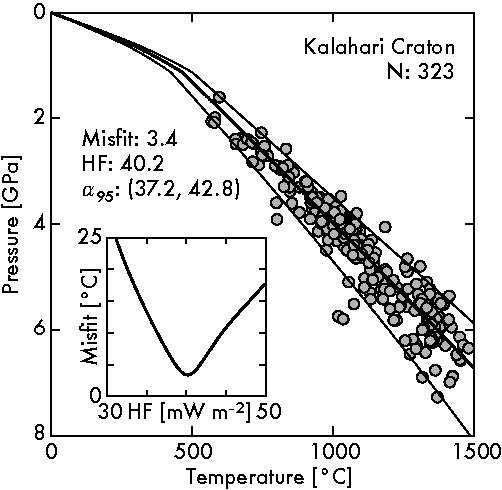
\includegraphics{geothermics/figures/kalahari.pdf}

        \textbf{Figure~\thefigure:} Geotherm for the Kalahari craton calibrated using xenolith $P$--$T$ estimates.
        \label{fig:kalahari}
    \end{center}

    The heat flow at the surface is due to the heat flowing into the base of the lithosphere (the limit of mantle convection) plus any additional heat produced within the lithosphere itself, which we can write,
    \[
        q_0 = q_{\mathrm{LAB}} + q_{\mathrm{sources}}.
    \]
    In general the contributions due to the mantle lithosphere and lower crust are relatively small and their variations have little effect on the geotherm.  Therefore, we can instead view the surface heat flow as the heat flow into the base of an radiogenic enriched layer, $q_{\mathrm{base}}$, and the heat produced within the HPE-enriched surface layer, $q_{\mathrm{uc}}$,
    \[
        q_0 = q_{\mathrm{base}} + q_{\mathrm{uc}}.
    \]

    For regions that have high heat flow, they may have high basal heat flow (input from the mantle), and/or high heat production.  We often assume that the heat production for regions of high heat production are some linear combination of the two, which we can write
    \[
        q_{\mathrm{base}} = P q_0, \quad \mathrm{and} \quad q_{\mathrm{uc}} = (1 - P) q_0,
    \]
    where $P$ is know as the partition coefficient.  From the latter equation, we can estimate the heat production.  We call geotherms parameterized by a single parameter, $P$, in this way a geotherm family.  One such family is shown in Figure~\ref{fig:cont} and provides a reasonable fit to the typical range of temperatures estimated within the continental lithosphere.
    \begin{center}
        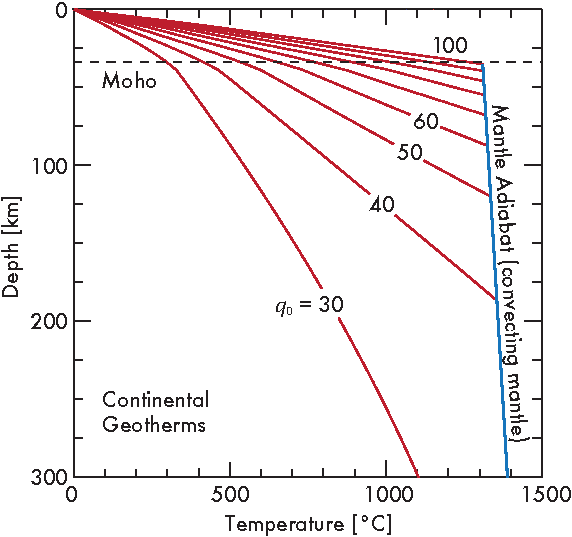
\includegraphics[]{geothermics/figures/continental_geotherms.pdf}

        \textbf{Figure~\thefigure:} A 1-D steady-state geotherm family parameterized in terms of surface heat flow.
        \label{fig:cont}
    \end{center}
}{aside}\label{box:reducedhf}

\subsection{Thermal Resistance}\label{sec:thermresist}
In many basins, the data that are used to estimate heat flow come from bottom hole temperatures (BHTs) in petroleum wells.  These temperatures are notoriously low quality, but with enough data and properly treated, they can give reasonable estimates of heat flow.  Although a basin may have many layers with different thicknesses and thermal conductivities we only need to compute the temperature at the location of the BHT measurement for modeling.  We use the thermal resistance method to compute the temperature at the level of a BHT without having to go through the process of computing the temperature at the base of each layer as outlined above.

To start this derivation, we assume heat generation is negligible, i.e., $A \approx 0$.  For most basins, the effect of heat generation on geothermal temperatures is minimal.  You can test this assumption by choosing a reasonable set of geothermal parameters and computing the heat production to the depth of a deep petroleum well.  Setting $A = 0$ allows us to write the layered model for the $i$-th layer:
\begin{equation}
  T_{i+1} = T_{i} + \frac{q_{i}}{k_{i+1}} (z_{i+1} - z_{i}).
\end{equation}
Since there is no heat generation, the conservation of energy tells us that the heat flowing into the base of each layer must be equivalent to the heat flowing out of the top of each layer.  It follows from this argument that the surface heat flow must be equivalent to the heat flow across each layer, i.e. $q_0 = q_i$ for all $i$.  Since the difference in depths between the bottom and top layer interfaces is the thickness of each layer as we have defined them, we can write the thickness, $h$, as $h_{i+1} = z_{i+1} - z_i$.  Hence, for the first few layers, we can write the temperature at the base of each as
\begin{align*}
    \text{Layer 1:} \quad T_1 &= T_0 + q_0 \frac{h_1}{k_1} , \\
    \text{Layer 2:} \quad T_2 &= T_1 + q_0 \frac{h_2}{k_2} ,  \\
    \text{Layer 3:} \quad T_3 &= T_2 + q_0 \frac{h_3}{k_3} .
\end{align*}
Substituting $T_1$ into the equation for $T_2$ above and then $T_2$ into $T_3$,
we find the temperature at the base of layer three can be written as
\begin{align*}
    T_3 &= \underbrace{
            \underbrace{T_0 + q_0 \frac{h_1}{k_1}}_{T_1}
            + q_0 \frac{h_2}{k_2}
        }_{T_2}
        + q_0 \frac{h_3}{k_3} \\
        &= T_0 + q_0 \left( \frac{h_1}{k_1} + \frac{h_2}{k_2} + \frac{h_3}{k_3}
        \right) \\
        &= T_0 + q_0 \sum_{i=1}^3 \frac{h_i}{k_i} .
\end{align*}
Generalizing the solution for the base of the $i$-th layer,
\begin{equation}
    T_{i} = T_{0} + q_{0} \sum_{i=1}^{N} \frac{h_i}{k_i} .
\end{equation}

This solution now allows us to solve for the temperature at the base of any given layer we wish without having to bootstrap our way from the surface to the depth of interest.  It also leads us to the implication that the effective thermal conductivity of a set of layers is equivalent to the harmonic mean of the conductivities, i.e.,
\begin{equation}
    k_{\mathrm{eff}} = \frac{\sum_{i=1}^N h_i}{\sum_{i=1}^N \frac{h_i}{k_i}} .
\end{equation}

\subsection{Temperatures of a buried sphere}

We have previously solved for the gravity and magnetic field for a buried sphere. In those cases, the sphere is embedded in a uniform background field, and the total field is obtained by superposition of the background and the sphere anomaly. The same principle applies in geothermics. Although the background temperature varies with depth, it is laterally uniform, so we may again decompose the solution into a background and a perturbation.

We consider a steady-state conductive medium containing a spherical body of radius $a$, centered at $(x,y,z) = (0,0,z_c)$. The governing equation is
\[
    k \laplacian T = -A,
\]
where thermal conductivity $k$ and heat production $A$ are piecewise constant:
\begin{align*}
    k &= k_\ell, \quad A = A_\ell \quad \text{(host medium)}, \\
    k &= k_s, \quad A = A_s \quad \text{(sphere)}.
\end{align*}

We decompose the temperature field as
\[
    T(\vb{x}) = T_\ell(z) + T'(\vb{x}),
\]
where $T_\ell(z)$ is the background solution (Equation~\ref{eq:ssgtherm}) and $T'$ is the perturbation due to the sphere.

\subsubsection*{Geometry and governing equations}

Let
\[
    R = \sqrt{x^2 + y^2 + (z - z_c)^2}, \qquad
    \cos\theta = \frac{z - z_c}{R}.
\]

Substituting $T = T_\ell + T'$ into $k_s \laplacian T = -A_s$ inside the sphere and using $k_\ell \laplacian T_\ell = -A_\ell$, the perturbation satisfies
\[
    \laplacian T' =
    \begin{dcases}
        -\Delta & R \leq a, \\
        0       & R > a,
    \end{dcases}
\]
where
\[
    \Delta = \frac{A_s}{k_s} - \frac{A_\ell}{k_\ell}
\]
is the effective source contrast.

The local background gradient at the sphere centre is
\[
    \Gamma = \eval{\dv{T_\ell}{z}}_{z=z_c}.
\]

\subsubsection*{General solution}

The axisymmetric solution that is bounded at $R=0$ and decays as $R\to\infty$ is
\[
    T' =
    \begin{dcases}
        \alpha + \beta\,(z - z_c) - \dfrac{\Delta}{6}\,R^2 & R \leq a, \\[6pt]
        \dfrac{\gamma}{R} + \delta\,\dfrac{z - z_c}{R^3} & R > a.
    \end{dcases}
\]

\subsubsection*{Boundary conditions at $R = a$}

Two conditions must hold simultaneously at the sphere surface:
\begin{enumerate}
    \item \emph{Continuity of temperature}: $T_{\mathrm{in}} = T_{\mathrm{out}}$, which is equivalent to $T'_{\mathrm{in}} = T'_{\mathrm{out}}$ since $T_\ell$ is continuous.
    \item \emph{Continuity of normal heat flux}: the physical condition is $k_s\,\partial T_{\mathrm{in}}/\partial R = k_\ell\,\partial T_{\mathrm{out}}/\partial R$.  Writing $T = T_\ell + T'$ and noting that $\partial T_\ell/\partial R = \Gamma \cos\theta$, this becomes a condition on the anomaly alone:
    \[
        k_s\,\pdv{T'_{\mathrm{in}}}{R}
        -
        k_\ell\,\pdv{T'_{\mathrm{out}}}{R}
        =
        (k_\ell - k_s)\,\Gamma \cos\theta.
    \]
\end{enumerate}

Separating monopole ($\ell=0$) and dipole ($\ell=1$) spherical harmonics and applying both conditions yields

\begin{alignat*}{2}
    \text{monopole:} \quad
    &\gamma = \frac{k_s\,\Delta\,a^3}{3k_\ell},
    &\qquad \alpha = \frac{\Delta\,a^2(k_\ell + 2k_s)}{6k_\ell}, \\[4pt]
    \text{dipole:} \quad
    &\delta = -\frac{(k_s - k_\ell)\,\Gamma \,a^3}{k_s + 2k_\ell},
    &\qquad \beta  = -\frac{(k_s - k_\ell)\,\Gamma}{k_s + 2k_\ell},
\end{alignat*}

with $\delta = \beta\,a^3$.  Substituting back confirms that both branches give identical values at $R = a$ for all $\theta$.

\subsubsection*{Surface heat flow anomaly}

Since the total surface heat flow is $q_s = q_\ell + q'$, the anomaly is found from the vertical derivative of $T'$ evaluated at $z = 0$:
\[
    q'(x,y) = k_\ell \eval{\pdv{T'}{z}}_{z=0},
\]
where $R_s = \sqrt{x^2 + y^2 + z_c^2}$ and $q'$ is upward positive.  Differentiating the exterior solution gives
\[
    q'(x,y)
    =
    \frac{k_s\,\Delta\,a^3}{3}\frac{z_c}{R_s^3}
    -
    k_\ell \left(\frac{k_s - k_\ell}{k_s + 2k_\ell}\right)
    \Gamma a^3
    \left(
        \frac{1}{R_s^3}
        - \frac{3 z_c^2}{R_s^5}
    \right).
\]

\subsubsection*{Interpretation}

The anomaly separates naturally into two contributions:
\begin{itemize}
    \item a monopole term proportional to $\Delta = A_s/k_s - A_\ell/k_\ell$, which decays as $R_s^{-3}$, and
    \item a dipole term proportional to $(k_s - k_\ell)$, which produces a sign change with radial distance and vanishes when conductivities are equal.
\end{itemize}
The monopole arises from the effective source contrast $\Delta$, which couples both heat production \emph{and} conductivity differences — a sphere with high heat production but proportionally high conductivity can have a suppressed monopole.  This behaviour is directly analogous to potential field problems, where source contrasts produce monopoles and property contrasts in a background field produce dipoles.

\section{Topographic Corrections to Steady-State Heat Flow}

Even in steady state, surface heat-flow measurements can be biased by topography.  Irregular ground surfaces distort near-surface isotherms, producing spatially variable temperature gradients that are unrelated to variations in deep thermal structure. These effects must be accounted for before interpreting heat-flow data in terms of lithospheric processes.

The influence of topography on conductive heat flow was analyzed in detail by \citet{Blackwell_etal1980}, who showed that terrain-induced distortions can be quantitatively corrected using Fourier methods closely analogous to those employed in gravity and magnetic continuation.

\subsection{Formulation}

We consider steady-state heat conduction in a homogeneous half-space,
\[
    \laplacian T = 0,
\]
with a non-planar surface described by a height function $z = h(x,y)$. At the surface, temperature is prescribed,
\begin{equation}
    T(x,y,h) = T_s(x,y),
\end{equation}
and temperature approaches a linear geotherm at depth.

Small topographic relief allows the problem to be linearized about a planar surface.  In this approximation, terrain effects act as a perturbation superimposed on the background geotherm.

\subsection{Fourier solution and terrain correction}

Expressing surface temperature or elevation as a two-dimensional Fourier series,
\begin{equation}
    h(x,y) = \sum_{\mathbf{k}} \hat{h}(\mathbf{k})
    \,e^{i\mathbf{k}\cdot\mathbf{x}},
\end{equation}
the corresponding temperature perturbation at depth $z$ takes the form
\begin{equation}
    T'(\mathbf{k},z) = \hat{T}_s(\mathbf{k}) \,e^{-|\mathbf{k}| z},
\end{equation}
where $\mathbf{k}$ is the horizontal wavenumber vector.

This exponential decay shows that high-wavenumber (short-wavelength) topographic features influence temperature only very near the surface, while long-wavelength relief penetrates more deeply. The mathematics is directly analogous to upward continuation in gravity and magnetics.

The apparent perturbation to heat flow is obtained by differentiating the temperature field,
\begin{equation}
    q'(\mathbf{k},z) =
    - k |\mathbf{k}| \hat{T}_s(\mathbf{k})
    \,e^{-|\mathbf{k}| z}.
\end{equation}

Topographic corrections are therefore computed by downward continuing the surface temperature or elevation field to the measurement depth and removing the resulting heat-flow perturbation from observed gradients.

\subsection{Interpretation and limitations}

Topographic effects are strongest in the upper 30--\SI{200}{m}, the depth interval over which most heat-flow measurements are made. Even in regions of modest relief, these effects can produce apparent gradient variations comparable to those caused by real lithological contrast.

Fourier-based corrections are particularly powerful because they:
\begin{itemize}
\item isolate wavelength-dependent effects,
\item clarify the depth-of-influence of topography,
\item and closely parallel techniques used in other potential-field methods.
\end{itemize}

At the same time, accurate correction requires realistic surface temperature boundary conditions. As emphasized by \citet{Blackwell_etal1980}, microclimatic effects related to slope, aspect, and elevation can be as important as the geometric surface relief itself.

\subsection{Context within steady-state geothermics}

Topographic corrections reinforce a central interpretive message of this chapter: even in steady state, observed thermal gradients reflect the combined influence of geometry, boundary conditions, and material properties. Removing terrain effects does not make the problem unique, but it reduces spurious complexity and clarifies which features require geological explanation.

Together with thermal refraction and heat-production trade-offs, terrain effects illustrate why careful forward modeling is essential before attempting inversion of heat-flow data.

\section{Summary of Steady-State Thermal Structure}

In this first half of the chapter we have developed steady-state thermal models of the lithosphere, beginning with the governing equation for conductive heat transport and examining how boundary conditions, material properties, and internal heat production shape the resulting temperature field.

A central lesson is that steady-state geotherms are strongly controlled by boundary conditions. Surface temperature and heat flow constrain the near-surface gradient, but they do not uniquely determine temperatures at depth. Lithospheric thickness emerges from the intersection of the conductive geotherm with the mantle adiabat, rather than being imposed directly.

We have also seen that internal heat production introduces curvature, layered conductivity produces thermal refraction, and surface geometry can distort otherwise simple gradients. Each of these effects illustrates the same fundamental point: steady-state heat flow measurements reflect an integrated response to geometry, material properties, and sources, rather than offering a direct or unique window into deep structure.

Steady-state solutions are therefore best understood as physically consistent reference states. They provide essential constraints and intuition, but they cannot by themselves resolve geological history or uniquely identify subsurface structure. These limitations motivate the explicit introduction of time dependence.

\clearpage
\nocite{Beardsmore&Cull2001}
\nocite{Carslaw&Jaeger1986}
\nocite{Fowler1990}
\nocite{Jaupart&Mareschal2011}
\nocite{Lowrie1997}

\bibliographystyle{elsarticle-harv}
\bibliography{ref}

\def\hfu{mW~m\ensuremath{^{-2}}}
\def\hgu{\ensuremath{\mu}W~m\ensuremath{^{-3}}}
\def\tcu{W~m\ensuremath{^{-1}}K\ensuremath{^{-1}}}
\chapter[Geothermics: Thermal Evolution and Transient Processes]{Geothermics\\ {\LARGE Thermal Evolution and Transient Processes}} \label{ch:geothermics2}

\section{Introduction}

The steady-state solutions developed above describe the long-time limit of conductive heat transfer. In many geological settings, however, the lithosphere has not reached thermal equilibrium. Surface temperatures change (climate change), boundaries move (sedimentation/erosion), phase changes occur (magmatism/metamorphism), and internal structure evolves (geodynamics). In these cases, temperature retains a finite memory of past conditions, and time becomes an essential variable.

In this second half of the chapter we return to the full diffusion equation,
\begin{equation}
\frac{\partial T}{\partial t} = \kappa \nabla^2 T + \mathrm{sources},
\end{equation}
and examine how thermal anomalies propagate, decay, and interact with boundary conditions. Unlike gravity and magnetics, where the response to sources is instantaneous, geothermics is intrinsically time-dependent. Thermal signals diffuse rather than propagate, and their influence diminishes systematically with time and depth.

Transient problems reveal how the solid Earth records surface temperature changes, sedimentation and erosion, latent heat associated with phase changes, and other time-dependent processes. They also clarify what information can be recovered from present-day thermal observations and what aspects of history are irretrievably lost.

Together, the steady-state and transient treatments form a unified framework for interpreting geothermal data. The steady-state solutions define reference structures and long-term averages; transient solutions describe departures from those states and the processes that produce them. Understanding both is essential before moving on to numerical modeling and inversion methods.

\ntextbox{Key Concepts}{
\small
\begin{itemize}
    \item \textbf{Geothermics directly measures and models a thermodynamic state variable: temperature.}
    
    Unlike other geophysical methods, which infer physical state through proxy responses
    (e.g., velocity, conductivity, or force fields), geothermics observes temperature
    itself and models its evolution explicitly.
    
    \textit{How does direct access to temperature shape what aspects of Earth history can be recovered?}


    \item \textbf{Thermal observations are integrative and history-dependent rather than imaging.}
    
    Transient temperature fields record the cumulative effects of past boundary
    conditions, internal processes, and material properties, filtered by diffusion.

    \textit{What geological information is retained by diffusion, and what information is irreversibly lost?}


    \item \textbf{Heat transport in the Earth is fundamentally diffusive and introduces long but finite memory.}
    
    Diffusion smooths spatial variations and causes present-day temperature fields to
    retain a decaying memory of past tectonic, magmatic, climatic, burial, and erosional
    events.

    \textit{How do characteristic diffusion timescales control what parts of Earth history remain thermally visible?}


    \item \textbf{Thermal diffusivity controls how rapidly temperatures respond to forcing.}
    
    The rate at which thermal anomalies propagate and decay is governed by diffusivity,
    which sets the depth and timescale of thermal memory.

    \textit{How does diffusivity limit temporal resolution in paleoclimate and burial histories?}


    \item \textbf{Surface boundary conditions impose time-dependent thermal forcing on the solid Earth.}
    
    Climatic change, sedimentation, erosion, and glaciation modify subsurface
    temperatures by altering surface temperature or translating the boundary through
    the thermal field.

    \textit{Over what depths and timescales do different surface processes influence subsurface temperatures?}


    \item \textbf{Cooling and heating are modified by phase changes and latent heat.}

    Melting, crystallization, dehydration, and solid-solid phase transitions absorb or
    release latent heat, slowing or accelerating thermal evolution and introducing
    moving thermal boundaries.

    \textit{How do phase changes alter cooling or heating rates without necessarily changing surface heat flow?}


    \item \textbf{Transient thermal models are inherently non-unique and require geological constraint.}

    Different thermal histories can produce similar present-day temperature profiles
    because diffusion smooths and attenuates past signals.
    
    \textit{Which aspects of thermal history are fundamentally unrecoverable, even with perfect data?}
\end{itemize}
}{core}

\section{Thermal Properties for Transient Problems}

\subsection{Heat Capacity, $\rho C_P$}
The heat storage capacity in rocks is determined by the product of the mass density, $\rho$, and the specific heat capacity at constant pressure, $C_P$. The specific heat capacity is a quantity indicating the amount of thermal energy (heat) required to raise one unit mass one degree.  While both parameters are pressure--temperature dependent, their product tends to be less sensitive to state than thermal conductivity.  As a result, variations in thermal storage tend to influence transient timescales more than steady-state geotherms, and only become first-order in problems involving rapid heating or cooling.
\begin{table}[tbhp]
    \centering
    \caption{Heat capacity for some selected rock types.}
    \label{tab:heatcapacity}
    \begin{tabular}{lccc}
        \toprule
        \textbf{Material} &
        \textbf{Density} & 
        \textbf{Specific heat capacity} & 
        \textbf{Volumetric heat capacity} \\
        & $\rho$ (\si{kg.m^{-3}}) &
        $C_P$ (\si{J.kg^{-1}.K^{-1}}) &
        $\rho C_P$ (\si{MJ.m^{-3}.K^{-1}}) \\
        \midrule
        brine & 1030--1300 & 3000--4000 & 3.5--4.5 \\
        granite & 2600--2700 & 750--900 & 2.0--2.4 \\
        diorite & 2750--2900 & 800--950 & 2.2--2.7 \\
        gabbro & 2900--3100 & 800--950 & 2.3--2.9 \\
        peridotite & 3300--3400 & 900--1050 & 3.0--3.5 \\
        amphibolite & 2950--3100 & 800--950 & 2.4--2.9 \\
        granulite & 2900--3100 & 800--950 & 2.3--2.9 \\
        gneiss & 2650--2850 & 800--950 & 2.1--2.7 \\
        \bottomrule
    \end{tabular}
\end{table}
Table~\ref{tab:heatcapacity} illustrates that, compared to thermal conductivity and radiogenic heat production, volumetric heat capacity varies over a relatively restricted range for most crustal and upper-mantle lithologies.

\subsection{Thermal Diffusivity, $\kappa$}
Thermal diffusivity is a derived property of materials and determined by
\begin{equation}
    \kappa = \frac{k}{\rho C_P}.
\end{equation}
As you will find in the transient solutions to the diffusion equation, thermal diffusivity controls the time scale for cooling/heating.  Higher diffusivities result a more rapid approach to equilibrium temperatures.  Thermal diffusivity therefore governs how quickly temperature perturbations decay over a given length scale, with low-diffusivity regions retaining thermal anomalies for longer periods of geological time.

Thermal diffusivity is compositionally dependent.  For common plutonic rocks, thermal conductivity and volumetric heat capacity vary systematically with composition but in opposite senses. Felsic rocks tend to exhibit higher thermal conductivity and lower volumetric heat capacity, whereas mafic rocks tend to exhibit lower conductivity and higher volumetric heat capacity. These trends compound, rather than cancel, leading to higher thermal diffusivities in felsic rocks and lower diffusivities in mafic rocks. Nevertheless, the overall range of diffusivity across common crustal lithologies remains modest compared to the much larger variability in conductivity and radiogenic heat production.  

\section{Transient geotherms}

To isolate the fundamental physics of time-dependent heat transport in the lithosphere, we begin with a simplified form of Equation~\ref{eq:heateq}. As in Section~\ref{sec:ss}, we adopt the following assumptions:
\begin{description}
    \item[Assumption 1:] no advection, $u = 0$;
    \item[Assumption 2:] ignoring sources, $A = 0$;
    \item[Assumption 3:] lateral heat flow is negligible $\displaystyle \pdv[2]{T}{x} = \pdv[2]{T}{y} = 0$; and
    \item[Assumption 4:] thermophysical properties are spatially uniform and constant in time, e.g., $\rho(x,y,z,t) = \rho$.
\end{description}
Under these conditions, the thermal evolution reduces to one-dimensional diffusion in the vertical direction:
\begin{equation}
    \pdv{T(z,t)}{t} = \kappa \pdv[2]{T(z,t)}{z},
\end{equation}
where $\kappa$ is the thermal diffusivity. This equation governs the transient adjustment of temperature profiles toward thermal equilibrium.

\subsection{Mathematical treatment of problems}

A well-posed transient thermal problem requires both:
\begin{itemize}
    \item an \textit{initial condition} specifying the temperature everywhere at $t=0$; and
    \item \textit{boundary conditions} specifying the behaviour of temperature or heat flux at the domain boundaries for $t>0$.
\end{itemize}

For a second-order spatial differential equation, two independent boundary conditions are required in the spatial coordinate. These are typically expressed as either:
\begin{itemize}
    \item fixed temperature (Dirichlet conditions), or
    \item fixed heat flow / temperature gradient (Neumann conditions).
\end{itemize}
In what follows, we develop solutions relevant to geophysical problems, focusing on cooling of a half-space and a finite-thickness plate, along with several extensions.

\ntextbox{Functional Solutions to PDEs}{
    \noindent The heat equation
    \[
    \pdv{T}{t} = \kappa \pdv[2]{T}{z}
    \]
    imposes a strong constraint on the form of acceptable solutions: the rate of change of temperature in time must be proportional to its spatial curvature. 

    This requirement severely limits the types of functions that can satisfy the equation. In particular, the second derivative in space must reproduce the original function up to a multiplicative constant. Functions with this property are especially useful because they preserve their form under differentiation.

    To make this concrete, consider a separable solution of the form $T(z,t) = Z(z)\,\Theta(t)$. Substituting into the heat equation gives
    \[
    \frac{1}{\Theta}\dv{\Theta}{t} = \kappa \frac{1}{Z}\dv[2]{Z}{z}.
    \]
    Since the left-hand side depends only on $t$ and the right-hand side only on $z$, both must equal a constant. The problem therefore reduces to solving ordinary differential equations whose solutions must reproduce themselves under differentiation.

    Functions with this property include trigonometric and exponential functions:
    \begin{align*}
        f(x) &= \sin(b x), &
        g(x) &= \cos(b x), &
        h(x) &= \exp(-b x) \\
        \dv[2]{f}{x} &= -b^2 \sin(b x), &
        \dv[2]{g}{x} &= -b^2 \cos(b x), &
        \dv[2]{h}{x} &= b^2 \exp(-b x).
    \end{align*}

    Because these functions reproduce themselves (up to a constant factor) under second differentiation, they form the natural building blocks for solutions to the heat equation. By combining them and enforcing the appropriate boundary and initial conditions, we can construct temperature fields for a wide range of transient geophysical problems.
}{mathtool}

\subsubsection{Fourier series}\label{sec:fseries}
Many thermal problems can be solved using Fourier series, which builds solutions by generating functions by using either sine or cosine equations.  The solutions to the PDE's are quite well known, all we need to do is determine the amplitude of each periodic function.  The mechanics of these solutions are discussed in Chapter~\ref{ch:fourier_series}.  Detailed below is a generalized solution when the temperature at the surface and base of a plate are fixed. These boundary conditions are know as the plate cooling model.

Suppose we wish to know the thermal evolution of a plate with thickness, $L$, in both space and time, i.e. $T(z,t)$.  Temperature is held constant at the top, $T(0,t) = T_0$, and at base of the plate, $T(L,t) = T_L$ and the temperatures throughout the plate can initially be described by a function of depth, $f(z)$ (Figure~\ref{fig:fsetup}).
\begin{figure}[hbt]
    \centering
    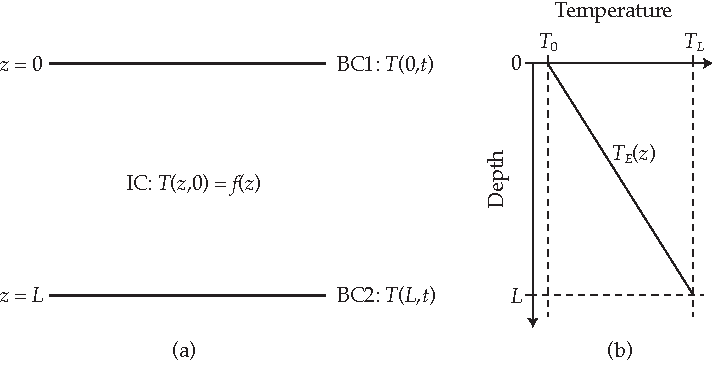
\includegraphics[]{geothermics/figures/fourier_setup.pdf}
    \caption{Model setup used to solve the 1-D, conductive, heat equation with
    fixed temperature boundary conditions and no internal heat sources.}
    \label{fig:fsetup}
\end{figure}

Another constraint we can place on the thermal evolution is the asymptotic temporal solution ($t \to \infty$). Since there are no sources in this model, the equilibrium solution, $T_E(z)$, satisfies $\pdv[2]{T_E}{z} = 0$.  We may also refer to the equilibrium solution as the steady-state solution.  For our chosen problem, the equilibrium solution is simply a linear temperature function between the fixed boundary temperatures,
\begin{equation}
    T_E(z) = T_0 + \frac{T_L - T_0}{L} z .
\end{equation}

We can define a displacement function as the difference between our desired solution and the equilibrium temperature,
\begin{equation}
    R(z,t) = T(z,t) - T_E(z) ,
    \label{eq:R}
\end{equation}
with boundary conditions $R = 0$ at $z = 0 and L$.  We can show that $\pdv{R}{t}
= \pdv{T}{t}$ and $\pdv[2]{R}{z} = \pdv[2]{T}{z}$, which means $R$ also satisfies
the heat equation,
\begin{equation}
    \pdv{R}{T} = \kappa \pdv[2]{R}{z} .
\end{equation}
It may seem like we haven't made much progress towards the solution we care about, $T(z,t)$, except that the solution to $R(z,t)$ is well known.  What we have done is turn our problem into one with differing boundary temperatures (inhomogeneous boundary conditions) to one with quite simple and equal boundary conditions (homogeneous boundary conditions).  Using a Fourier series, we can write the solution to $R(z,t)$ as
\begin{equation}
    R(z,t) = \sum_{n=1}^{\infty} a_n \sin \left( \frac{n \pi z}{L} \right)
    \exp \left( -\frac{ n^2 \pi^2 }{L^2} \kappa t \right)
    \label{eq:Rsoln}
\end{equation}
Equating~\ref{eq:R} and \ref{eq:Rsoln},
\begin{equation}
    T(z,t) - T_E(z) = \sum_{n=1}^{\infty} a_n \sin \left( \frac{n \pi z}{L} \right)
    \exp \left( -\frac{ n^2 \pi^2 }{L^2} \kappa t \right) ,
    \label{eq:Tsoln}
\end{equation}
and applying the initial condition, $T(z,0) = f(z)$, we find
\begin{equation*}
    f(z) - T_E(z) = \sum_{n=1}^{\infty} a_n \sin \left( \frac{n \pi z}{L} \right)
\end{equation*}
where the Fourier coefficients, $a_n$ are found by
\begin{equation}
    a_n = \frac{2}{L} \int_0^L [f(z) - T_E(z)] \sin \left( \frac{n \pi z}{L}
    \right) \dd{z} .
    \label{eq:fcoef}
\end{equation}

Finally, rearranging Equation~\ref{eq:Tsoln} we find
\begin{equation}
    T(z,t) =  T_E(z) + \sum_{n=1}^{\infty} a_n \sin \left( \frac{n \pi z}{L} \right)
    \exp \left( -\frac{ n^2 \pi^2 }{L^2} \kappa t \right) .
\end{equation}

Now all we need to know is the initial condition in order to find the Fourier coefficients using Equation~\ref{eq:fcoef} and to compute the temperature as the system cools.  The versatility of such a solution is the range of initial conditions that we can supply and the range of problems that can be solved.  While the problems are likely to be quite simple physically, they can still provide useful insight into the variations of temperature, heat flow, subsidence and characteristic cooling scales that we can reasonably expect for physical processes acting within the Earth.

%----------------------------------------------------------
\subsection{Half-space model}

The half-space cooling model provides one of the simplest and most widely applicable solutions to the heat equation. It describes the thermal evolution of a semi-infinite medium that undergoes a sudden change in surface temperature. Because no intrinsic length scale is imposed, the solution depends only on the combined variable $\eta = z / (2\sqrt{\kappa t})$, reflecting the diffusive nature of heat transport.

This model is relevant to a wide range of geophysical problems, including the cooling of newly formed oceanic lithosphere, the thermal evolution of lava flows and lava lakes before cooling reaches their base, and any situation in which heat diffuses into (or out of) a medium that is effectively infinite laterally and vertically over the timescale of interest.

\subsubsection{Derivation}

For simple half-space cooling, we assume the surface temperature is held constant and the entire Earth is at some mantle temperature.  Cooling of a half-space with constant thermal properties and no internal heat production is determined by solving the PDE discussed above,
\[
    \pdv{T}{t} = \kappa \pdv[2]{T}{z} .
\]
The boundary and initial conditions are given by
\begin{align*}
    \text{BC:} \quad T(0,t) &= T_0 , \\
    \lim_{z \to \infty} T(z,t) &= T_a , \\
    \text{IC:} \quad T(z,0) &= T_a,
\end{align*}
To solve this PDE (a function of time and space), we will turn it into an ODE (a function of one variable).  To do so, we will introduce a non-dimensional parameter and a new non-dimensional temperature,
\begin{align*}
    \eta &= z / 2 \sqrt{\kappa t} , \\
    \theta(\eta) &= \frac{T(z,t) - T_0}{T_a - T_0},
\end{align*}
which allows us to write,
\[
    -\eta \dv{\theta}{\eta} = \frac{1}{2} \dv[2]{\theta}{\eta} ,
\]
with a single boundary condition $\theta(0) = 0$.  The solution to this PDE is well known,
\[
    \theta(\eta) = \erf (\eta) ,
\]
where $\erf (x)$ is the error function,
$\frac{2}{\sqrt{\pi}}\int_0^{x} e^{-\xi^{2}} \dd{\xi}$ (Box~\ref{box:erf}).

Next, we merely substitute for our non-dimensional parameters and solve for the temperature function,
\begin{equation}
T(z,t) = T_0 + (T_a - T_0) \erf \left( \frac{z}{2 \sqrt{\kappa t}} \right),
\end{equation}

\begin{figure}[hbtp]
    \centering
    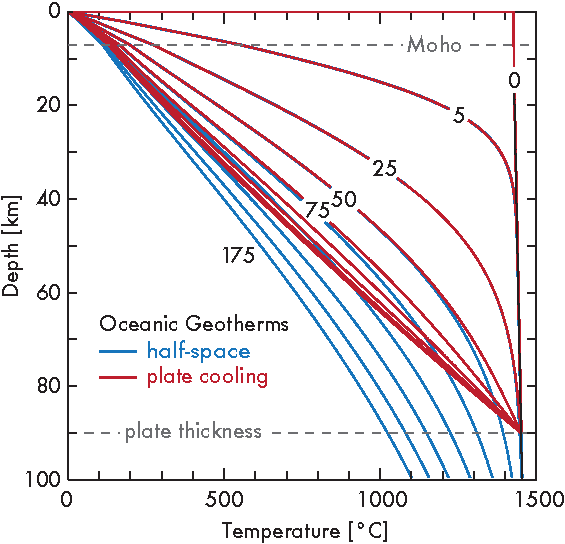
\includegraphics[]{geothermics/figures/oceanic_geotherms.pdf}
    \caption{Temperature solutions to the 1-D half-space and plate cooling
    models applicable to the oceanic lithosphere.}
    \label{fig:og}
\end{figure}

For transient problems, the surface heat flow is not constant but can be calculated as a function of time using Fourier's Law,
\begin{equation}
    q_{0}(t) = \frac{k (T_{a} - T_{0})}{\sqrt{\pi \kappa t}}.
\end{equation}

%Rocks, like most materials, expand when heated (or contract when cooled) and
%experience a change in density as a result
%\begin{equation}
%    \rho(T) = \rho_0 [1 + \alpha (T - T_0)],
%\end{equation}
%where $\rho_0$ is the reference density, measured at the reference temperature,
%T_0$.

Rocks, like most materials, expand when heated (or contract when cooled) and as a result, experience a change in density.  This change in density affect the overall buoyancy of the lithosphere and using the principles of isostasy we can solve for this subsidence.

The subsidence, $s$, is a little more difficult to compute (since it involves integration) but arises from balancing isostatic columns.  The density variations result from the thermal contraction the lithosphere and the in-filling density of water above the cooler column.  Subsidence can be computed using
\begin{equation}
    s(t) = \frac{\rho_{m}}{\rho_{m} - \rho_{w}} \alpha
        \int_{0}^{\infty} [ T(z,0) - T(z,t) ] \dd{z},
    \label{eq-subsidence}
\end{equation}
where $\rho_{w}$ and $\rho_{m}$ are seawater and mantle density, respectively.  The volumetric expansivity is given by $\alpha$, and the initial geotherm is $T(z,0)$.  Temperature is integrated from the surface to the depth of compensation, which is infinite in the case of a half-space.  The subsidence for half-space cooling is given by
\begin{equation}
    s(t) = \frac{2 \rho_{m} \alpha (T_{m} - T_{0})}
        {(\rho_{m} - \rho_{w})}\sqrt{\frac{\kappa t}{\pi}}.
\end{equation}
\begin{figure}[hbtp]
    \centering
    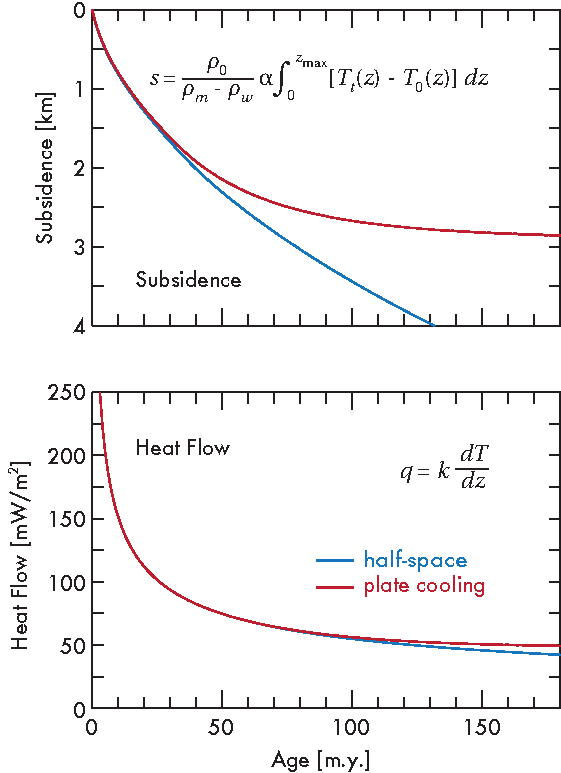
\includegraphics[]{geothermics/figures/oceanic_tis.pdf}
    \caption{Subsidence and heat flow as a function of age.}
    \label{fig:otis}
\end{figure}

\subsubsection{Thermal Length and Diffusion Time}
Often in physics, we try to make estimates for some scale (e.g.\ distance, time) related to a process without having to perform (or in advance of) an experiment.

For transient thermal processes we can examine the argument of the error function.  The argument of the error function must be unitless (much like the arguments of $\exp$, $\log$, and trigonometric functions).  We define one thermal length when the argument of the error function is equal to 1 (i.e., $\erf (1)$).  Hence the thermal length is given by
\begin{equation}
  z = 2 \sqrt{\kappa t},
\end{equation}
and represents the depth at which $\sim$16\% of the change in temperature from $T_{a}$ to $T_0$ is observed.  We can also use this relationship to estimate the time at which the propagating thermal wave can be felt at a given distance from the temperature perturbation,
\begin{equation}
    t = \frac{z^2}{4 \kappa} ,
\end{equation}
wich is know as the diffusion or characteristic time.

% ----- Error function -----
\ntextbox{Error Function}{
    The error function derives its name from applications in probability and statistics.  However, the error function is a common within many solutions to the heat equation.  The error function is defined as
    \begin{equation*}
        \erf (x) = \frac{2}{\sqrt{\pi}}\int_{0}^{x} e^{-\xi^{2}} \dd{\xi}.
    \end{equation*}
    The error function is an odd function (i.e.\ $\erf (-x) = - \erf (x))$ where
    \begin{align*}
        \erf (0) & = 0 \\
        \lim_{x \to \infty} \erf (x) = 1.
    \end{align*}

    Some solutions to the heat equation require the complementary error function,
    \begin{align*}
        \erfc (x) & = 1 - \erf(x) \\
        \erf (x) & = \frac{2}{\sqrt{\pi}}\int_{x}^{\infty} e^{-\xi^{2}} \dd{\xi}.
    \end{align*}

    We typically use the point at which the argument of the error function is equal to unity (i.e.\ $\erf (1)$) to estimate parameters such as the time it takes to cool to a given depth or the depth cooling has reached in a given time.  At $\erf (1) \approx 0.8427$, 16\% of the temperature step has occurred.

    \begin{center}
        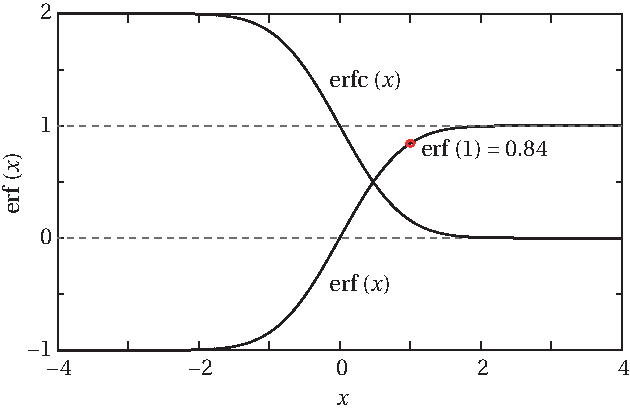
\includegraphics[]{geothermics/figures/erf.eps}
        \captionof{figure}{The error function and its complement.}
        \label{fig:erf}
    \end{center}

    The error function is reasonably linear to an argument of $\sim$0.75 and then rapidly asymptotes towards 1.  By an argument of 3, the result is 0.9999779\ldots.
    \begin{center}
    \captionof{table}{The error function values as a function of the argument.}
    \label{tab:erf}
    \begin{tabular}{@{}cccccc@{}}
        \toprule
        \textbf{argument}, $x$ & $\erf(x)$ & $\erfc(x)$ & $x$ & $\erf(x)$ & $\erfc(x)$ \\
        \midrule
        -3.0000 &  $\sim$-1.0000 &  $\sim$2.0000 &   0 &  0       &   1.0000 \\
        -2.5000 &  -0.9996 &   1.9996 &   0.1000  &  0.1125  &   0.8875 \\
        -2.0000 &  -0.9953 &   1.9953 &   0.2000  &  0.2227  &   0.7773 \\
        -1.7500 &  -0.9867 &   1.9867 &   0.3000  &  0.3286  &   0.6714 \\
        -1.5000 &  -0.9661 &   1.9661 &   0.4000  &  0.4284  &   0.5716 \\
        -1.2500 &  -0.9229 &   1.9229 &   0.5000  &  0.5205  &   0.4795 \\
        -1.0000 &  -0.8427 &   1.8427 &   0.6000  &  0.6039  &   0.3961 \\
        -0.9000 &  -0.7969 &   1.7969 &   0.7000  &  0.6778  &   0.3222 \\
        -0.8000 &  -0.7421 &   1.7421 &   0.8000  &  0.7421  &   0.2579 \\
        -0.7000 &  -0.6778 &   1.6778 &   0.9000  &  0.7969  &   0.2031 \\
        -0.6000 &  -0.6039 &   1.6039 &   1.0000  &  0.8427  &   0.1573 \\
        -0.5000 &  -0.5205 &   1.5205 &   1.2500  &  0.9229  &   0.0771 \\
        -0.4000 &  -0.4284 &   1.4284 &   1.5000  &  0.9661  &   0.0339 \\
        -0.3000 &  -0.3286 &   1.3286 &   1.7500  &  0.9867  &   0.0133 \\
        -0.2000 &  -0.2227 &   1.2227 &   2.0000  &  0.9953  &   0.0047 \\
        -0.1000 &  -0.1125 &   1.1125 &   2.5000  &  0.9996  &   0.0004 \\
        0       &  0.0000  &   1.0000 &   3.0000  &  $\sim$1.0000  &   $\sim$0.0000 \\
        \bottomrule
    \end{tabular}
\end{center}
}{mathtool}\label{box:erf}

\subsection{Plate Cooling}

While the half-space solution provides a useful first-order description of lithospheric cooling, it does not reproduce the observed long-term behaviour of the ocean basins. In particular, both seafloor subsidence and surface heat flow decrease rapidly at young ages but tend to level off in older lithosphere. This flattening suggests that cooling is limited by a process not captured by the half-space model.

An alternative framework, proposed by \citet{McKenzie1967}, is the plate cooling model. The key difference between the two models lies in the basal boundary condition: the half-space model assumes an infinite domain, whereas the plate model imposes a finite lithospheric thickness with a fixed temperature at its base (Figure \ref{fig:plate}). This constraint limits the growth of the thermal boundary layer and leads to a more realistic long-term thermal evolution of oceanic plates.

This 1-D solution and the 2-D version of this problem are used to model the temperature, heat flow, and subsidence of the oceanic lithosphere. Note the spreading velocity only matters when plate velocities fall below $\sim\SI{10}{mm.a^{-1}}$, so the 1-D model is generally sufficient.
\begin{figure}[hbtp]
  \centering
  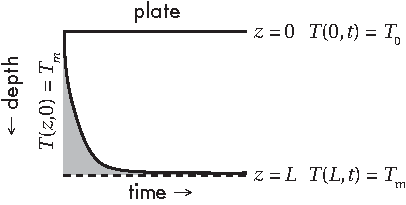
\includegraphics[]{geothermics/figures/platesetup.pdf}
  \caption{Plate model setup.}
  \label{fig:plate}
\end{figure}

\ntextbox{Derivation of Fourier Coefficients for Plate Cooling}{
    The solution consists of two parts, a constant gradient term representing the asymptotic solution and the Fourier series of a function that, when combined, the two parts give the initial condition as discussed in Section~\ref{sec:fseries} above.  The initial condition is a constant temperature throughout the plate, $f(z) = T_m$.  The equilibrium condition is a linear solution from the surface to the maximum depth of the plate $L$, 
    \[
        T_E = T_0 + (T_m - T_0)L^{-1}z .
    \]
    To find the Fourier coefficients for this problem we use Equation~\ref{eq:fcoef} and substitude in the initial and equilibrium functions,
    \begin{align*}
        a_n &= \frac{2}{L} \int_0^L \left[T_m - T_0 + \frac{T_m - T_0}{L} z \right]
        \sin \left( \frac{n \pi z}{L} \right) \dd{z} \\
        &= \frac{2}{L} \int_0^L (T_m - T_0) \left(1 + \frac{z}{L} \right)
        \sin \left( \frac{n \pi z}{L} \right) \dd{z}.
    \end{align*}
    We can break the integral up into two separate integrals to evaluate separately
    \[
        a_n = \frac{2(T_m - T_0)}{L} \Biggl(
        \underbrace{\int_0^L \sin \left( \frac{n \pi z}{L} \right)
        \dd{z}}_\text{\ding{202}} +
        \frac{1}{L}\underbrace{\int_0^L z \sin \left( \frac{n \pi z}{L} \right)
        \dd{z}}_\text{\ding{203}} \Biggr)
        .
    \]
    To solve each integral, we employ $u$-substitution with
    \begin{align*}
        u &= \frac{n \pi z}{L} \\
        \dd{u} &= \frac{n \pi}{L} \dd{z} \\
        \text{lower limit:}&\text{ at } z = 0, u = 0 \\
        \text{upper limit:}&\text{ at } z = L, u = n \pi .
    \end{align*}
    For \ding{202} the resulting integral is
    \begin{align*}
        \int_0^L \sin \left( \frac{n \pi z}{L} \right) \dd{z}
        &= \frac{L}{n \pi} \int_0^{n \pi}  \sin u \dd{u} \\
        &= \left. - \frac{L}{n \pi} \cos u \dd{u} \right|_{0}^{n \pi} \\
        &= - \frac{L}{n \pi} (\cos (n\pi) - 1) .
    \end{align*}
    Since $n$ is an integer, $\cos u$ is either -1 or 1 depending upon $n$ being either odd or even, respectively.  To say this another way, $\cos(n\pi) = (-1)^n$. And so \ding{202} becomes
    \[
        \frac{L}{n \pi}((-1)^n + 1)
    \]
    Following a similar process for \ding{203} the resulting integral is
    \begin{align*}
        \int_0^L z \sin \left( \frac{n \pi z}{L} \right) \dd{z} &= 
        \frac{L^2}{n^2 \pi^2} \int_0^{n \pi} u \sin u \dd{u} \\
        &= \frac{L^2}{n^2 \pi^2} \left. \sin u \right|_0^{n\pi} - \left. u \cos u \right|_0^{n\pi} \\
        &= \frac{L^2}{n^2 \pi^2} \sin (n\pi) - \sin 0 - (n\pi \cos(n\pi) - 0 \cos 0) \\
        &= - \frac{L^2}{n^2 \pi^2} n \pi \cos(n\pi) \\
        &= - \frac{L^2}{n \pi} (-1)^n .
    \end{align*}

    Substituting the resulting expressions from \ding{202} and \ding{203} back into $a_n$ and simplifying
    \[
        a_n = \frac{2 (T_m - T_0)}{L} \left( \frac{L}{n \pi}[(-1)^n + 1] -
        \frac{1}{L} \frac{L^2}{n \pi} (-1)^n \right)
    \]
    we find the value of the Fourier coefficients for the plate cooling model are given by
    \[
        a_n = \frac{2(T_m - T_0)}{n \pi} .
    \]
}{core}\label{box:platecooling}
\FloatBarrier

\subsubsection{Solution}
Temperatures for the plate cooling model can be estimated from the following relation,
\begin{equation}
    \workeq
    T(z,t) = T_{0} - (T_{m} - T_{0})
    \left[\frac{z}{L} + \frac{2}{\pi}\sum_{n = 1}^{\infty}
    \frac{1}{n} \sin\left(\frac{n \pi z}{L}\right)
    \exp\left(- \frac{n^2 \pi^2 \kappa t}{L^2}\right) \right].
    \label{eq:plateT}
\end{equation}
Heat flow is given by
\begin{equation}
    q_{0}(t) = k \eval{\pdv{T}{z}}_{z=0} = 
    \frac{k (T_{m} - T_{0})}{L}
    \left[ 
        1 + 2 \sum_{n = 1}^{\infty} \exp\left( -\frac{n^2 \pi^2 \kappa t}{L^2}\right)
    \right],
    \label{eq:plateq}
\end{equation}
and the subsidence is found by
\[
    s(t) = \frac{\rho_m \alpha}{\rho_m - \rho_w}\int_0^L \left[T(z,t) - T_m\right] \dd{z}
\]
which after integration of $T(z,t)$ yields
\begin{equation}
    s(t) = \frac{\rho_{m} \alpha (T_{m} - T_{0}) L}{2 (\rho_{m} - \rho_{w})}
        \left[ 1 - \frac{8}{\pi^2} \sum_{n = 0}^{\infty} \frac{1}{(2n + 1)^2}
        \exp\left( -\frac{(2n + 1)^2 \pi^2 \kappa t}{L^2} \right) \right].
    \label{eq:plates}
\end{equation}
\begin{figure}[hbtp]
  \centering
  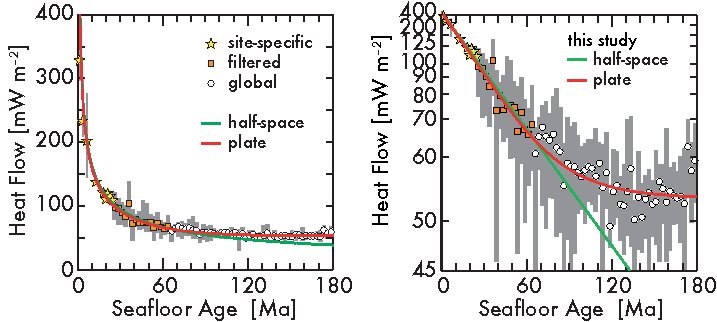
\includegraphics{geothermics/figures/hfage.pdf}
  \caption{Plate (red) and half-space (green) cooling models fit to oceanic heat flow data.  Both plots illustrate the same result with the linear scales and on the left and (heat flow)$^{-2}$ on the right to illustrate the differences between the heat flow and age relationships for the two cooling models.}
  \label{fig-hfage}
\end{figure}
While the solution to each of these is an infinite sum, we can approximate the solution by setting an acceptable tolerance for the error in the solution (or changes between successive terms within the sum).

\subsubsection{Time and Depth Scales}

The solution to the plate cooling model can be laborious to compute but we can develop two separate approximations that simplify the computations considerably.  Examining the argument of the exponential from the solution for heat flow of a plate (Equation~\ref{eq:plateq}) we can define the characteristic time as
\begin{equation}
    \tau = \frac{L^2}{\kappa},
\end{equation}
which has the units of time.

At the early-stages of cooling ($t \ll \tau$), the heat loss is essentially the same as the half-space cooling model, which can be approximated by
\begin{equation}
    q_{0}(t) \approx \frac{k (T_{m} - T_{0})}{\sqrt{\pi \kappa t}}.
\end{equation}

For late-stage cooling ($t \gg \tau$), the heat loss can be approximated by only the first term ($n = 1$) of the summed term in Equation~\ref{eq:plateq},
\begin{equation}
    q_{0}(t) \approx \frac{k (T_{m} - T_{0})}{L}
        \left[ 1 + 2 \exp\left( -\frac{\pi^2 \kappa t}{L^2}\right) \right].
\end{equation}

At very long time periods, the heat flow approaches an asymptotic value
\begin{equation}
    \lim_{t \to \infty} q_{0}(t) = \frac{k (T_{m} - T_{0})}{L}.
\end{equation}


\subsection{1-D Transient Solutions}\label{sec:fseries}

Let us consider how to solve problems such as the plate cooling model below, but for slightly more complicated cases (i.e. ones in which the temperature is not initially constant).  We will be exploring the transient heat flow equation without sources
\begin{equation}
    \pdv{T}{t} = \kappa \pdv[2]{T}{z} .
\end{equation}
The boundary and initial conditions are given by
\begin{align}
    \textbf{BC:} \quad T(0,t) &= T_0 , \\
    T(L,t) &= T_L , \\
    \textbf{IC:} \quad T(z,0) &= f(z),
\end{align}
where $f(z)$ is an arbitrary function of temperature as a function of depth.  For the plate cooling model above, $f(z) = T_L$.  We cannot solve this problem directly because the boundary conditions are not homogeneous (i.e. $T_0 \neq T_L$).  So we need to look for a way to rewrite---at least part---of this problem with homogeneous boundary conditions.

To reformulate our problem, we will subtract the equilibrium solution from the transient solution to give the problem homogeneous boundary conditions.  The equilibrium temperature distribution is given by Laplace's equation,
\begin{equation}
    \pdv[2]{T_E}{z} = 0 ,
\end{equation}
with the boundary conditions:
\begin{align}
    T_E(0) &= T_0 , \\
    T_E(L) &= T_L .
\end{align}
Since there are no sources we can easily guess the equilibrium solution,
\begin{equation}
    T_E(z) = T_0 + \frac{T_L - T_0}{L} z .
\end{equation}

To continue reformulating our problem, we will look at the transient cooling as a displacement from equilibrium.  To do this, all we need to do is define the displacement temperature as
\begin{equation}
    \theta(z,t) \equiv T(z,t) - T_E(z) .
\end{equation}
From this definition, it follows that
\begin{equation}
    \pdv{\theta}{t} = k \pdv[2]{\theta}{z} ,
\end{equation}
and subtracting the equilibrium boundary and initial conditions from those
of our original transient PDE,
\begin{align}
    \text{BC:} \quad \theta(0,t) &= 0 , \\
    \theta(L,t) &= 0 , \\
    \text{IC:} \quad \theta(z,0) &= f(z) - T_E(z) .
\end{align}

Now that we have a PDE with homogeneous boundary conditions we can solve the PDE using the standard separation of variables
\begin{equation}
    \theta(z,t) = \sum_{n=1}^\infty a_n \sin \left( \frac{n \pi z}{L} \right)
    \exp \left( - \frac{n^2 \pi^2}{L^2} \kappa t \right) .
\end{equation}
The initial conditions imply,
\begin{equation*}
    f(z) - T_E = \sum_{n=1}^\infty a_n \sin \left( \frac{n \pi z}{L} \right) ,
\end{equation*}
hence the Fourier coefficients are given by
\begin{equation}
    a_n = \frac{2}{L} 
        \int_0^L [f(z) - T_E(z)] \sin \left( \frac{n \pi z}{L} \right) \dd{z} .
\end{equation}

Now that we have solved for the Fourier coefficients we can calculate the transient cooling using our previous definition of $\theta(z,t)$
\begin{equation}
    T(z,t) = T_E(z) + \theta(z),
\end{equation}
with the full solution,
\begin{equation}
    T(z,t) = T_E(z) + \sum_{n=1}^\infty a_n \sin \left( \frac{n \pi z}{L}
    \right) \exp \left( - \frac{n^2 \pi^2}{L^2} \kappa t \right) .
\end{equation}

If the heat production is independent of time, we can also use this method to solve
\begin{equation}
    \pdv{T}{t} = \kappa \pdv[2]{T}{z} + \frac{A(z)}{\rho C_P} .
\end{equation}


\section{Cooling Involving Phase Changes}\label{sec:stefan}

Phase changes introduce latent heat into thermal problems, fundamentally altering how temperature evolves through time. Unlike purely conductive problems with fixed boundaries, latent heat problems involve \emph{moving internal boundaries} whose positions must be solved as part of the problem.

Such problems are referred to as \emph{Stefan problems} and are characterized by:
\begin{itemize}
    \item heat diffusion in each phase,
    \item a moving phase boundary,
    \item and an energy balance at that boundary that accounts for latent heat.
\end{itemize}

In this section we derive two classical examples relevant to igneous systems:
the cooling of a tabular dike and the cooling of a spherical pluton.

\subsection{Cooling of a Dike}

Consider a planar igneous dike intruded into cooler country rock. The dike
solidifies inward from its margins as heat is conducted away. We idealize the
problem as one-dimensional and symmetric about the dike center.

Let $x$ denote distance normal to the dike, with $x=0$ at the center. The solid--
liquid interface is located at $x = \pm s(t)$, where $s(t)$ is an unknown function
of time. Temperature evolves by conduction in both the solid and liquid regions,
\[
    \pdv{T}{t} = \kappa \pdv[2]{T}{x}.
\]

We impose:
\begin{align*}
    \text{BC1:}\quad T(x,0) &= T_0 \qquad \text{for } |x| < s(0), \\
    \text{BC2:}\quad T(x,t) &\rightarrow T_\infty \qquad \text{as } |x| \rightarrow \infty.
\end{align*}

The phase boundary is constrained to be at the melting temperature,
\[
    T(x = s(t)) = T_m .
\]

By symmetry,
\begin{equation}
    \eval{\pdv{T}{x}}_{x=0} = 0.
\end{equation}

The key physical constraint enters through conservation of energy at the moving
interface. As the solidification front advances, latent heat is released at a rate
proportional to the speed of the interface. This heat must be conducted away through the surrounding solid. Balancing these effects at the propagating boundary yields the Stefan condition,
\begin{equation}
    \rho L \frac{ds}{dt} = - k \eval{\pdv{T}{x}}_{x = s(t)^-},
\end{equation}
where $L$ is the latent heat of fusion per unit mass.

The coupled system admits a similarity solution in which the position of the
solidification front evolves as
\begin{equation}
    s(t) = 2 \lambda \sqrt{\kappa t},
\end{equation}
with the dimensionless constant $\lambda$ determined implicitly by the Stefan
condition. The essential result is that the interface advances proportional to
$\sqrt{t}$ rather than linearly in time. Latent heat therefore acts to slow cooling: energy extracted from the system is consumed by phase change rather than temperature reduction. The $\lambda$ parameter is not analytic, but can be determined by the transcendental equation arising from the Stefan condition:
\begin{equation}
    \workeq
    \lambda e^{\lambda^2} \erf (\lambda) = \frac{L}{C_P (T_m - T_\infty)}.
\end{equation}

The key result is that the solidification front advances as
\[
    s(t) \propto \sqrt{t},
\]
not linearly in time. Latent heat slows cooling by requiring that energy be removed
to change phase rather than temperature. Large latent heat or small temperature
contrast leads to slow crystallization.

%----------------------------------------------------------
\subsection{Cooling of a Spherical Pluton}

We now consider the solidification of a spherical pluton of radius $R$, surrounded
by cooler country rock. In contrast to the dike, curvature plays an essential role.

Let $r$ denote radial distance from the pluton center, and let $r = s(t)$ denote the solidification front.

\subsubsection*{Governing equation}

In spherical symmetry, the diffusion equation takes the form:
\begin{equation}
    \frac{\partial T}{\partial t} =
    \kappa \left( \frac{1}{r^2}\pdv{}{r} \left( r^2 \pdv{T}{r} \right) \right).
\end{equation}

\subsubsection*{Boundary and Initial Conditions}

At the center,
\begin{equation}
\left.\frac{\partial T}{\partial r}\right|_{r=0} = 0.
\end{equation}

At large distances,
\begin{equation}
T(r,t) \rightarrow T_\infty \quad \text{as } r \rightarrow \infty.
\end{equation}

The phase boundary satisfies
\begin{equation}
T\bigl(r = s(t)\bigr) = T_m.
\end{equation}

\subsubsection*{Stefan condition for a sphere}

Energy conservation at the moving boundary requires
\begin{equation}
\rho L \frac{ds}{dt} = - k \eval{ \pdv{T}{r} }_{r=s(t)^-}.
\end{equation}

The mathematical form is identical to the planar case, but the temperature gradient
now reflects spherical geometry.

\subsubsection*{Similarity form}

As in the planar Stefan problem, the solution admits a similarity form
\begin{equation}
s(t) = 2 \lambda \sqrt{\kappa t},
\end{equation}
but the value of $\lambda$ differs because the diffusion operator is different.

The solidification front again advances proportional to $\sqrt{t}$, but cooling is
more efficient than in the planar case because curvature enhances heat loss.

\subsubsection*{Comparison with the dike problem}

\begin{itemize}
\item Both problems exhibit $s(t) \propto \sqrt{t}$ behavior.
\item Latent heat controls the pace of solidification in both geometries.
\item Spherical plutons cool faster than planar dikes for the same material
properties due to geometric heat focusing.
\end{itemize}

\subsection{Metamorphic Reaction Fronts}

Metamorphic reaction fronts also release or absorb latent heat and propagate through rock, but unlike igneous solidification they are typically coupled to reaction kinetics and mass transport. Whether such fronts admit analytical solutions depends on the simplifications adopted and will be considered separately.
\begin{itemize}
    \item Show how cooling/heating rates are modified
    \item Emphasize that temperature evolution != heat flow evolution
    \item New conceptual depth without heavy math

    \item Note that the signal is superimposed on the background (solid Earth) thermal gradient
    \item Depth of penetration
    \item Timescale dependence
\end{itemize}

%----------------------------------------------------------
\section{Climatic Forcing of the Solid Earth}

Until now, we have assumed that the surface temperature of Earth is a constant value.  While this assumption is fine for the construction of crustal and lithospheric scale geotherms it is clearly not constant as we ourselves respond to the yearly and daily variations.  These atomospheric variations affect ground surface temperatures.  Ground surface temperatures vary through time on a wide range of timescales, from daily and seasonal cycles to glacial-interglacial transitions and long-term climate change.  Because the solid Earth responds to thermal forcing by diffusion, these variations propagate downward from the surface, modifying subsurface temperatures without destroying the underlying conductive structure.

In this section, we examine how surface temperature variability acts as a time-dependent boundary condition on the thermal diffusion equation, how the resulting signals decay with depth, and what geological consequences follow from these processes.

\subsection{Downward propagation of thermal signals}

The temperature evolution in the shallow crust in response to a ground surface temperature change is governed by the one-dimensional diffusion equation,
\begin{equation}
    \frac{\partial T}{\partial t} = \kappa \frac{\partial^2 T}{\partial z^2},
\end{equation}
where $z$ is depth measured downward from the surface. When surface temperature varies in time, it enters the problem as a time-dependent boundary condition,
\begin{equation}
    T(0,t) = T_s(t).
\end{equation}
The ground surface temperature variations are superimposed on top of the background thermal gradient.  Hence, it is useful to decompose the temperature field into a steady-state background geotherm and a transient perturbation,
\begin{equation}
    T(z,t) = T_\Gamma(z) + T'(z,t),
\end{equation}
where $T_\Gamma(z)$ satisfies the steady-state equation and $T'(z,t)$ represents the climatically forced signal. Because the diffusion equation is linear, these components superimpose without interacting: climatic signals modify temperatures but do not erase the background thermal gradient of the solid Earth.

A key feature of diffusion is that the depth to which a thermal signal penetrates depends on its characteristic timescale. Short-period signals are confined to shallow depths, while long-period signals diffuse more deeply. This timescale dependence is made explicit by examining a simple analytic solution.

%----------------------------------------------------------
\subsection{Surface boundary condition variability}

\subsubsection*{Periodic forcing: daily and annual thermal waves}

Consider the case of sinusoidal surface temperature forcing,
\begin{equation}
    T_s(t) = T_{\mathrm{mean}} + T_a \cos(\omega t),
\end{equation}
where $T_a$ is the amplitude and $\omega = 2\pi/\tau$ is the angular frequency associated with period $\tau$.

We seek solutions of the form
\begin{equation}
    T'(z,t) = \Re\left\{ \hat{T}(z) e^{i\omega t} \right\},
\end{equation}
which, when substituted into the diffusion equation, yields
\begin{equation}
    \frac{d^2 \hat{T}}{dz^2} - \frac{i\omega}{\kappa} \hat{T} = 0.
\end{equation}

The physically acceptable solution that decays with depth is
\begin{equation}
    T'(z,t) = T_a e^{-z/\delta} \cos\!\left(\omega t - \frac{z}{\delta}\right),
\end{equation}
where the characteristic decay length
\begin{equation}
    \delta = \sqrt{\frac{2\kappa}{\omega}} = \sqrt{\frac{\kappa \tau}{\pi}}
\end{equation}
is known as the \emph{thermal skin depth}.

This result shows explicitly where the skin-depth scaling comes from. The amplitude of the temperature signal decays exponentially with depth, and the phase of the signal is delayed in proportion to depth. Both effects are controlled entirely by thermal diffusivity and the forcing period.

For diurnal forcing, the skin depth is of order tens of centimeters; for annual forcing, it is several meters. These shallow depths reflect the short timescales of the imposed surface variability.

\subsubsection*{Recent climate change}

Surface temperature changes associated with recent climate change act on decadal to
centennial timescales, corresponding to skin depths of hundreds of meters. Although
the surface perturbation is small compared to absolute temperatures at depth, its
signature can be resolved by subtracting the background geotherm.

This motivates the definition of a reduced temperature,
\begin{equation}
T_r(z,t) = T(z,t) - T_\Gamma(z),
\end{equation}
which isolates the transient climatic signal. Reduced temperature profiles measured
in boreholes provide a direct record of recent surface temperature history.

\subsection{Step changes in surface temperature}

While periodic forcing is useful for developing intuition, most climatic changes of geological interest are better approximated as step changes in surface temperature.  Examples include rapid post-glacial warming or abrupt climatic transitions inferred from proxy records. Step forcing leads to solutions that differ qualitatively from sinusoidal thermal waves and form the basis of most paleoclimate corrections applied to borehole data.

We consider the one-dimensional diffusion equation,
\begin{equation}
    \pdv{T}{t} = \kappa \pdv[2]{T}{z},
\end{equation}
with a surface boundary condition representing an instantaneous temperature change at time $t=0$,
\begin{equation}
    T(0,t) =
    \begin{cases}
        T_\Gamma, & t < 0, \\
        T_\Gamma + \Delta T, & t \ge 0.
    \end{cases}
\end{equation}
We seek the reduced temperature
\begin{equation}
    T_r(z,t) = T(z,t) - T_\Gamma(z),
\end{equation}
which isolates the transient perturbation relative to the steady background geotherm.

\subsubsection*{Green's function solution}

The solution for a step change in surface temperature can be constructed from the
fundamental solution (Green's function) of the diffusion equation. For an impulsive
surface temperature change, the reduced temperature at depth is
\begin{equation}
    T_r(z,t) = \Delta T \, \erfc \!\left( \frac{z}{\sqrt{4\kappa t}} \right),
\end{equation}
where $\operatorname{erfc}$ is the complementary error function.

This expression gives the instantaneous response to a permanent surface temperature
offset but does not yet represent the form typically used in paleoclimate studies,
which consider the *integrated* effect of the imposed surface step.

Integrating the surface forcing in time yields the physically relevant solution for a persistent step change,
\begin{equation}
    T_r(z,t) =
    \Delta T
    \left[ (1 + 2\xi^2)\,\erfc (\xi) - \frac{2\xi}{\sqrt{\pi}} e^{-\xi^2} \right],
    \qquad
    \xi = \frac{z}{\sqrt{4\kappa t}}.
\end{equation}
This expression is the forward kernel commonly used in borehole paleoclimate analysis.  It decays smoothly with depth and exhibits a characteristic curvature that depends explicitly on the time since the surface temperature change.

\subsubsection*{Penetration depth and timescale}

The argument of the error function makes clear that the relevant nondimensional depth is
\begin{equation}
    \xi = \frac{z}{\sqrt{4\kappa t}},
\end{equation}
from which the thermal penetration depth follows immediately as
\begin{equation}
    \delta \sim \sqrt{\kappa t}.
\end{equation}
This scaling is consistent with the skin depth derived for periodic forcing, but here it arises from the transient diffusion of a step boundary condition rather than a thermal wave.

\subsubsection*{Ice ages and interglacials}

Glacial-interglacial cycles act over timescales of $10^4$--$10^5$ years and therefore penetrate kilometers into the crust. Ice is an especially effective thermal boundary condition because it both fixes surface temperature near the pressure-melting point and persists long enough for diffusion to transmit the signal deeply.

As a result, glaciated regions retain a thermal memory of past ice cover long after deglaciation, influencing present-day geothermal gradients and shallow crustal temperatures.

\subsection{Paleoclimate corrections to geotherms}

Because borehole temperatures are influenced by past surface conditions, steady-state geotherms inferred from shallow temperature data must often be corrected for paleoclimate effects. The goal of such corrections is not to infer the full climate history, but to remove its influence in order to recover the underlying conductive geotherm.

This is accomplished by modeling surface temperature history as a series of step changes or continuous variations, computing the resulting transient temperature field using the diffusion equation, and subtracting this transient from the observed temperature profile. The corrected profile then more accurately reflects present-day heat flow and lithospheric structure.

Paleoclimate corrections work because diffusion preserves linearity and superposition: the temperature field retains a separable memory of boundary condition changes that can be modeled independently of the steady background state.

\subsection{Paleoclimate series of steps}

Real climatic histories are not single step changes but sequences of warming and cooling events. Because the diffusion equation is linear, the response to an arbitrary surface temperature history can be constructed by superposition of individual steps.

Suppose the surface temperature history is approximated as a series of step changes $\Delta T_i$ occurring at times $t = \tau_i$ before present. The reduced temperature profile is then
\begin{equation}
    T_r(z) = \sum_i \Delta T_i \, G\!\left( \frac{z}{\sqrt{4\kappa \tau_i}} \right),
\end{equation}
where $G(\xi)$ is the step-response kernel,
\begin{equation}
    G(\xi) =
    (1 + 2\xi^2)\,\erfc (\xi) - \frac{2\xi}{\sqrt{\pi}} e^{-\xi^2}.
\end{equation}

Each step contributes a smooth, depth-dependent temperature anomaly whose amplitude and curvature depend on the magnitude of the surface change and the time elapsed since it occurred. Older climatic events influence deeper temperatures, while recent events dominate the shallow profile.

\subsubsection*{Connection to inverse methods}

In paleoclimate reconstruction from borehole data, the step amplitudes $\Delta T_i$ and their ages $\tau_i$ may be treated as unknown parameters. Linearization of the forward model yields a Jacobian matrix whose columns correspond to partial derivatives of $T_r(z)$ with respect to these parameters.

Because the kernel $G(\xi)$ is analytic and smooth, its derivatives can be computed explicitly, enabling efficient Newton or Gauss-Newton inversion. The resulting inverse problem is moderately ill-posed, reflecting the diffusive smoothing inherent in the physics, but remains robust when regularized appropriately.

\subsection{Interpretation}

Step-change solutions emphasize several physically important points. Thermal diffusion strongly smooths surface temperature history, limiting temporal resolution at depth.  The subsurface retains a memory of past climates, but that memory degrades systematically with both depth and time. Paleoclimate corrections therefore recover broad temperature trends rather than sharp events.

From a conceptual standpoint, surface temperature history acts as a boundary control on a diffusive system, reinforcing the view of temperature as a state variable that integrates past forcing rather than responding instantaneously.

\subsection{Geological consequences}

Surface temperature variability has geological consequences despite its shallow expression. Permafrost formation and degradation are governed by the competition between climatic forcing and diffusive heat transport, linking ground ice stability directly to timescale.

Glacial-interglacial transitions also modify subsurface temperatures beneath ice sheets, altering geothermal gradients and interacting with glacial loading and unloading.  Although mechanical effects dominate isostatic responses, thermal diffusion controls the evolution of temperature-dependent material properties in the shallow crust.

More broadly, surface temperature variability produces a non-steady shallow thermal structure that departs systematically from steady-state geotherms. This reinforces several core concepts developed earlier in the chapter: temperature is a state variable, transient signals are diffusive rather than advective, and the system retains memory of past boundary conditions.

Climatic forcing therefore provides a powerful, intuitive example of diffusion in action, linking surface processes to subsurface thermal structure and emphasizing the time-dependent nature of the solid Earth's thermal state.

\section{Sedimentation and Erosion as Transient Thermal Forcing}

In addition to changes in surface temperature, vertical motion of the Earth's surface itself introduces transient thermal effects. Sedimentation buries isotherms and tends to suppress near-surface thermal gradients, while erosion exhumes warmer material and steepens them. These effects are well documented in marine and continental settings and were analyzed classically by \citet{VonHerzen&Uyeda1963}, who showed that sediment accumulation can significantly bias heat-flow measurements if not accounted for.

Unlike climatic forcing, sedimentation and erosion modify the thermal structure not by changing temperature at a fixed boundary, but by translating the boundary through the temperature field. This distinction makes them especially instructive examples of diffusion-controlled transients.

\subsection{Problem formulation}

Consider one-dimensional heat conduction in a medium undergoing vertical motion at a constant rate $v$, positive for sedimentation and negative for erosion. In a reference frame fixed to the solid Earth, the temperature obeys
\begin{equation}
\frac{\partial T}{\partial t}
=
\kappa \frac{\partial^2 T}{\partial z^2}
-
v \frac{\partial T}{\partial z},
\end{equation}
where the final term represents advection of isotherms due to surface motion.

Equivalently, the problem may be formulated as pure diffusion with a moving surface boundary,
\begin{equation}
z_s(t) = v t,
\end{equation}
on which temperature is fixed.

These two descriptions are mathematically equivalent and emphasize that sedimentation and erosion are fundamentally kinematic boundary-condition problems rather than internal heat-source effects.

\subsection{Thermal effect of steady sedimentation}

For steady sedimentation, new material is added at the surface with temperature $T_s$. Initially, the subsurface temperature field corresponds to a steady geotherm.  As sediment accumulates, isotherms are buried faster than diffusion can restore the steady gradient.

The characteristic competition is between:
\begin{itemize}
\item the burial timescale $\tau_b = z / v$, and
\item the diffusive timescale $\tau_d = z^2 / \kappa$.
\end{itemize}

Thermal effects become significant when $\tau_b \lesssim \tau_d$, or equivalently when
\begin{equation}
v \gtrsim \frac{\kappa}{z}.
\end{equation}

Under these conditions, the near-surface thermal gradient is reduced relative to the steady-state value, and heat flow inferred from shallow measurements is systematically underestimated. This mechanism explains many of the anomalously low heat-flow values observed in rapidly sedimenting marine basins \citep{VonHerzen&Uyeda1963}.

\subsection{Erosion and exhumation}

Erosion produces the opposite effect. Removal of material exposes warmer isotherms, steepening the near-surface thermal gradient. During rapid exhumation, heat flow measured near the surface may be transiently elevated even though the deep thermal structure remains unchanged.

From a thermal perspective, erosion is the time-reverse of sedimentation: the same governing equations apply, but with $v < 0$. This symmetry emphasizes that the thermal response depends on rates and timescales rather than on the geological process itself.

\subsection{Implications for heat-flow measurements}

Sedimentation and erosion directly affect the interpretation of heat-flow data because measurements are typically made over the upper few to tens of meters, precisely where these transient effects are strongest. Without correction, shallow gradients may not represent the long-term conductive heat flow.

Von Herzen and Uyeda demonstrated that even modest sedimentation rates can suppress measured heat flow for timescales comparable to the accumulation history. The thermal structure retains a memory of sedimentation that decays only diffusively, much like climatic forcing.

\subsection{Interpretive perspective}

Sedimentation and erosion reinforce several central ideas developed in this chapter.  Thermal structure reflects not only present conditions but the integrated history of boundary motion. Temperature is a state variable with finite memory. And observed heat flow must be interpreted in light of geological context rather than treated as a direct probe of deep thermal structure.

Together with climatic forcing, sedimentation provides a compelling demonstration that many apparent heat-flow anomalies arise not from anomalous heat sources, but from transient processes acting at the Earth's surface.

\subsection{Analytic solutions for sedimentation and erosion}

The thermal effects of sedimentation and erosion can be quantified analytically for simple cases. These solutions make explicit how vertical surface motion biases temperature gradients and heat-flow estimates.

\subsubsection*{Steady sedimentation or erosion}

Consider steady sedimentation or erosion at a constant vertical rate $v$, with $v>0$ for sedimentation and $v<0$ for erosion. In a reference frame fixed to the solid Earth, temperature satisfies the advection--diffusion equation
\begin{equation}
\frac{\partial T}{\partial t}
=
\kappa \frac{\partial^2 T}{\partial z^2}
-
v \frac{\partial T}{\partial z}.
\end{equation}

In the long-time limit, the system approaches a steady state in which temperature depends only on depth. The solution for the geothermal gradient is
\begin{equation}
    \frac{dT}{dz} =
    \left(\frac{q_0}{k}\right) \exp\!\left(-\frac{v z}{\kappa}\right),
\end{equation}
where $q_0$ is the true conductive heat flow at depth. The apparent heat flow inferred from a gradient measured at depth $z$ is therefore
\begin{equation}
    q_{\mathrm{app}}(z) = q_0 \exp\!\left(-\frac{v z}{\kappa}\right).
\end{equation}

For sedimentation ($v>0$), shallow gradients are suppressed and heat flow is systematically underestimated. For erosion ($v<0$), gradients are enhanced and heat flow is overestimated. The effect grows exponentially with burial or exhumation depth.

\subsubsection*{Transient onset of sedimentation}

More commonly, sedimentation begins at some finite time in the past. Suppose that steady sedimentation at rate $v$ begins at time $t=0$, applied to an initially steady geotherm. The resulting temperature anomaly relative to the original geotherm is
\begin{equation}
    T'(z,t) = -\frac{q_0}{k} \frac{\kappa}{v}
    \left[
    \exp\!\left(-\frac{v z}{\kappa}\right)
    \erfc\!\left( \frac{z - v t}{2\sqrt{\kappa t}} \right) -
    \erfc \!\left( \frac{z}{2\sqrt{\kappa t}} \right)
    \right].
\end{equation}

At early times, the disturbance is confined to shallow depths. As time increases, the burial signal propagates downward diffusively, while the exponential factor imposes the characteristic suppression of gradients associated with steady motion.

\subsubsection*{Finite sedimentary layer emplacement}

Sedimentary basins are often better approximated by emplacement of a sedimentary layer of thickness $H$ over a finite interval. If a layer of thickness $H$ is added instantaneously with surface temperature $T_s$, the resulting temperature anomaly is equivalent to a downward translation of the thermal field,
\begin{equation}
T'(z,t) =
T_0(z-H,t) - T_0(z),
\end{equation}
with subsequent diffusion smoothing the perturbation on the timescale $t \sim H^2/\kappa$.

This formulation highlights that sedimentation and erosion primarily act by translating existing thermal structure rather than generating new heat.

\subsubsection*{Interpretive implications}

These solutions make clear why sedimentation and erosion must be accounted for when interpreting heat-flow measurements. Even modest rates can distort shallow gradients over geological timescales. The thermal imprint of surface motion decays only diffusively, leaving a memory that persists long after sedimentation or erosion ceases.

Sedimentation and erosion therefore represent a third major class of transient thermal forcing, alongside surface temperature change and latent heat, completing the conceptual framework developed in this chapter.

%----------------------------------------------------------
\section{Non-Uniqueness and Interpretation}

The preceding sections demonstrate that a wide range of thermal models can satisfy the same set of surface observations. This non-uniqueness is not a deficiency of geothermics, but a fundamental consequence of diffusion, limited data, and incomplete knowledge of subsurface structure. Interpretation therefore requires explicit recognition of trade-offs and the incorporation of independent geological constraints.

\subsection{Trade-offs}

Perhaps the most common trade-off in geothermics is between heat production and thermal conductivity. A given surface heat flow can be explained by high internal heat production combined with high conductivity, or by lower heat production paired with low conductivity. Because surface heat flow constrains only the integrated thermal resistance and internal heating, these effects cannot be uniquely separated from thermal data alone.

A related ambiguity exists between boundary conditions and internal sources. Changes in basal mantle temperature can produce thermal effects similar to those caused by variations in crustal heat production. Likewise, transient surface temperature changes may alter shallow gradients in ways that mimic changes in material properties.

Global datasets of heat flow, crustal structure, and radiogenic element distribution provide critical constraints and reduce the range of acceptable models. However, these datasets do not eliminate ambiguity. \emph{These global datasets reduce ambiguity, but do not eliminate it.} This limitation reinforces three central themes: inversion is inherently non-unique, geological information is essential, and even the best global compilations must be interpreted cautiously.

\subsection{Role of geological constraints}

Because geothermics alone cannot determine unique subsurface structure, interpretation must be guided by independent geological constraints. Lithology controls thermal conductivity and heat production; tectonic history influences lithospheric thickness and basal temperature; and petrology governs phase changes and rheological behavior.

This role for geology mirrors that in gravity and magnetic interpretation. In all potential-field methods, physics constrains admissible solutions, but geology selects among them. Model credibility arises not from mathematical optimality alone but from consistency with known structure, composition, and tectonic evolution.

Seen in this light, thermal models are best understood not as definitive solutions, but as physically plausible realizations conditioned by both observations and geological reasoning.

\section{Forward Modeling and Numerical Methods}

Throughout this chapter, analytic solutions have played a central role. They clarify physical mechanisms, reveal scaling relationships, and provide benchmarks against which more complex models can be tested. At the same time, their limitations point directly toward numerical methods.

Analytic solutions---steady-state geotherms, Stefan problems, and transient surface forcing---establish essential intuition. They demonstrate how curvature reflects internal heat sources, how moving boundaries arise from latent heat, and how thermal signals diffuse with time. These solutions also provide reference cases for validating numerical implementations.

Most geological situations of interest involve complex geometry, spatially variable properties, nonlinear rheology, or coupled processes that cannot be treated analytically. In such cases, forward modeling using finite differences or related numerical methods becomes necessary.

The governing equations introduced here carry over directly: the diffusion equation, appropriate boundary conditions, and conservation laws remain unchanged. What changes is how they are solved.

Analytic solutions are necessarily idealized. They assume simple geometry, linear material behavior, and often constant properties. While invaluable for understanding, they cannot capture many important aspects of real Earth systems. A full treatment of numerical methods is therefore deferred to Chapter~\ref{ch:finitediff}, where these limitations are addressed explicitly.

\section{Concluding Remarks}

Geothermics occupies a distinctive position among geophysical methods. Its governing equations are time-dependent, its signals diffuse rather than propagate, and its memory of past conditions decays systematically with time and depth. These characteristics shape both what can be measured and how it must be interpreted.

The methods developed in this chapter provide a foundation for forward modeling and inversion using finite differences. They also establish natural connections to other fields. Temperature influences rheology and therefore lithospheric strength. It controls electrical conductivity, linking geothermics to electromagnetic methods. It determines magnetic mineral stability through the Curie temperature, coupling thermal structure to magnetic observations.

Geothermics thus serves not only as a tool for estimating temperatures, but as a bridge linking physical processes, geological history, and multiple geophysical observables within a unified framework.

\ntextbox{Comparison of potential fields}{
    In \emph{gravity}, present-day density contrasts and structure dominate the signal, and geological history is expressed indirectly through the architecture of the crust and isostatic response. In \emph{magnetics}, history is often more explicitly recorded through remanence, mineralogical state, and alteration, allowing evolutionary processes to be resolved in ways not possible with gravity alone. In \emph{geothermics}, geometry-based models explain mean thermal structure well, but spatial and temporal variations reflect diffusion, boundary conditions, and active processes, with memory that decays systematically over time and depth.  \emph{Electrostatics} differs from gravity, magnetics, and geothermics in that it is commonly implemented as an active-source technique, providing a conceptual bridge from passive potential-field methods to time-dependent electromagnetic geophysics.

    We can summarize these differences as:
    \begin{enumerate}
        \item \textbf{Gravity}
        \begin{description}
            \item[Governing equation:] elliptic (Poisson / Laplace)
            \item[Response:] instantaneous
            \item[Time dependence:] none
            \item[Memory:] none
            \item[Source:] passive
            \item[History:] appears only insofar as it has produced present-day density structure or in decaying isostatic disequilibrium
        \end{description}

        \item \textbf{Magnetics}
        \begin{description}
            \item[Governing equation:] elliptic (Poisson / Laplace, static limit)
            \item[Response:] instantaneous
            \item[Time dependence:] none in the field
            \item[Memory:] none in the field, but may exist in the source (remanence)
            \item[Source:] passive
            \item[History:] can be encoded directly in remanent magnetization (paleomagnetism)
        \end{description}

        \item \textbf{Geothermics}
        \begin{description}
            \item[Governing equation:] parabolic (diffusion) in general
            \item[Response:] intrinsic time-dependent
            \item[Memory:] finite and decaying
            \item[\emph{Long-time limit:}] reduces to an elliptic (steady-state) problem
            \item[Source:] passive
            \item[History:] transiently through thermal anomalies; persistently through boundary conditions and internal heat sources
        \end{description}

        \item \textbf{Electrostatics}
        \begin{description}
            \item[Governing equation:] elliptic (Poisson / Laplace)
            \item[Response:] instantaneous
            \item[Time dependence:] none in the static limit
            \item[Memory:] none in the field
            \item[Source:] active / passive
            \item[History:] expressed only through present-day conductivity structure or natural source terms (self-potential); most applications rely on imposed active sources
        \end{description}
    \end{enumerate}
}{aside}

\clearpage
\nocite{Beardsmore&Cull2001}
\nocite{Carslaw&Jaeger1986}
\nocite{Fowler1990}
\nocite{Jaupart&Mareschal2011}
\nocite{Lowrie1997}

\bibliographystyle{elsarticle-harv}
\bibliography{ref}
\chapter{Electrostatics}\label{ch:electrostatics}

\section{Introduction}
Electrostatics occupies a distinctive position in geophysics. Like gravity and magnetics, it is governed by an elliptic potential-field equation in the steady state and can be formulated entirely in terms of scalar potentials and boundary-value problems. Unlike gravity, magnetics, and geothermics, however, most electrostatic measurements in geophysics rely on active sources, in which currents are deliberately injected into the Earth and the resulting electric potentials are observed. This distinction between passive and active methods is as important conceptually as the distinction between elliptic and parabolic governing equations.

In its steady-state form, electrostatics provides a natural bridge between potential-field methods and time-dependent electromagnetic techniques. Electrical potential, current flow, and conductivity can be treated using the same mathematical framework as other elliptic problems, while making explicit how material properties control field behavior. When time dependence is introduced, electrostatics transitions directly into electromagnetic diffusion, forming the conceptual foundation for transient EM and frequency-domain methods such as magnetotellurics.

This chapter introduces electrostatics with a deliberately limited scope. The goal is not to develop a full exploration methodology, but to establish the physical and mathematical ideas needed to understand how electrical methods connect to gravity, magnetics, geothermics, and ultimately to electromagnetic geophysics. In this sense, electrostatics functions as a conceptual bridge rather than a stand-alone field method.

This role should be understood in the context of the comparison of potential fields introduced at the end of the geothermics chapter, where electrostatics marks the transition from passive field observations to controlled, active-source probing of Earth structure.


\ntextbox{Key Concepts}{
    \begin{itemize}
        \item \textbf{Electrostatics is governed by an elliptic potential-field equation in the steady state.}
        Electrical potentials satisfy Poisson's or Laplace's equation, placing electrostatics on the same mathematical footing as gravity and magnetics under equilibrium conditions.

        \item \textbf{Most electrostatic measurements in geophysics are active-source techniques.}
        Currents are deliberately injected into the Earth, and observed potentials reflect the Earth's response to controlled forcing rather than natural fields.

        \item \textbf{Electrical conductivity is the primary material property controlling electrostatic responses.}
        Variations in lithology, porosity, fluid content, and temperature govern current flow and potential distributions.

        \item \textbf{Electrostatic fields respond instantaneously to changes in current distribution.}
        In the static limit there is no intrinsic temporal memory in the field, and observed potentials represent a snapshot of present-day conditions.

        \item \textbf{Electrostatics provides the steady-state limit of electromagnetic problems.}
        When time dependence is introduced, electrostatic formulations transition naturally to electromagnetic diffusion.

        \item \textbf{Self-potential is the primary passive electrostatic method in geophysics.}
        Natural electrical sources such as fluid flow, redox reactions, and thermal gradients generate measurable electric potentials without imposed currents.

        \item \textbf{Electrostatics clarifies the distinction between potential-field methods and EM geophysics.}
        It highlights which aspects of EM behavior arise from time dependence rather than from the underlying physics of electrical conduction.
    \end{itemize}
}{core}

\section{Mathematical symbols and units}
Electric potentials and fields
Definitions of electric potential, electric field, and current density

\section{Constitutive relations and material properties}
Ohm's law, conductivity, and geological controls on electrical properties

\section{Governing equations}
Poisson's and Laplace's equations for electrostatics; boundary-value formulation

\section{Active-source electrostatics}
Conceptual treatment of current injection, potential measurements, and common geometries

\section{Passive electrostatics: self-potential}
Natural sources of electric potentials and geological interpretations

\section{Connection to electromagnetic diffusion}
From steady-state electrostatics to time-dependent EM problems

\section{Relationship to other geophysical methods}
Comparison with gravity, magnetics, and geothermics; passive vs active methods

\section{Looking Ahead}
Transition to transient EM, frequency-domain methods, and magnetotellurics
This chapter is intentionally compact and conceptual, serving as a foundation for electromagnetic methods rather than a comprehensive treatment of electrical exploration.

% Diffusion (mostly)
% Electromagnetics
\chapter{Electromagnetic Methods}\label{ch:EMmethods}

\section{Key Concepts}
\begin{itemize}
    \item Maxwell's equations (at least in a general way, e.g., Gauss's law of electricity states that the electric field on an enclosed surface is related to the charges contained within the volume enclosed by that surface and Faraday's law suggests that a time varying magnetic field causes a spatial change in the electric field.) Note all del (upside down triangle) denotes is a spatial variation in a parameter one way or another.

    \item What are the wave equation, diffusion equation, and Helmholtz
    equations. What assumptions help define them (e.g., for magnetic induction we assume the conductivity is ? than the electric permittivity).

    \item What is the difference between a time domain and frequency domain
    method?

    \item What is magnetic induction (you should be able to express this in
    words as well as a simple equation)?

    \item What are the implications of the circuit analogy (i.e., what are the
    currents in the conductor and receiver sensitive to and how do they relate
    to the resistivity of the Earth)?

    \item What are skin depth, characteristic impedance, apparent resistivity,
    surface impedance (and how are they calculated\ldots)?

    \item What are the 1-D generalizations for MT?

    \item What are electrical conductivities of typical earth materials?  How do
    we estimate effective conductivity for mixed phases?
\end{itemize}

\section{Mathematical symbols and units}
\begin{table}[hbt]
    \centering
    \begin{threeparttable}
    \caption{Definitions of symbols.\vspace{2pt}}
    \label{tab:emsym}
    \begin{tabular}{@{}cll@{}}
        \toprule
        Symbol &
        Quantity &
        SI Unit \\
        \midrule
        $t$             & time                          & second, \si{s} \\
        $x$, $y$, $z$   & distance                      & meter, \si{m} \\
        $\tau$          & period                        & s \\
        $f$             & frequency                     & hertz, \si{s^{-1}} \\
        $\omega$        & angular frequency ($\omega = 2 \pi f$) & \si{rad.s^{-1}} \\
        $\lambda$       & wavelength                    & \si{m} \\
        $k$             & wavenumber ($k = 2\pi \lambda^{-1}$)
            & radians m$^{-1}$ \\

        $q$ ($Q$)       & single (total) electric charge    & coulomb, \si{C} \\
        $\rho_{f}$      & electric charge density       & \si{C.m^{-2}} \\
        $U$, $V$        & electric potential, voltage   & volt, \si{V} \\
        $\mathcal{E}$      & electromotive force           & V \\
        $I$             & electric current              & ampere, $\si{A} = \si{C.s^{-1}}$ \\
        $R$             & resistance                    & ohm, \si{\Omega} \\
        $L$             & inductance                    & henry, \si{H} \\
        $C$             & capacitance                   & farad, \si{F} \\
        $Z$             & complex impedance             & \si{\Omega} \\

        $\vb{D}$       & electric displacement/flux density    & \si{C.m^{-2}} \\
        $\vb{E}$       & electric field strength       & \si{V.m^{-1}} \\
        $\vb{B}$       & magnetic induction/flux density   & tesla,
            \si{T} = \si{Wb.m^{-2}} = \si{V.s.m^{-2}} \\
        $\vb{H}$       & magnetic field strength       & \si{A.m^{-1}} \\
        $\Phi_{B}$      & magnetic flux                 & weber, $\si{Wb} = \si{V.s}$ \\
        $\vb{J}$       & electric current density      & \si{A.m^{-2}} \\

        $\rho$          & electrical resistivity        & \si{\Omega.m} \\
        $\sigma$        & electric conductivity         & \si{S.m^{-1}}; 
        siemens, $\si{S} = \si{\Omega^{-1}}$ \\
        $\epsilon$      & electrical permittivity, dielectric constant &
        \si{F.m^{-1}} \\
        $\mu$           & magnetic permeability         & \si{H.m^{-1}} \\
        \bottomrule
    \end{tabular}
    \begin{tablenotes}
        \item Notes: Scalar quantities are written as $B$, while vectors are written as $\vb{B}$.
        \item The unit of conductance, \si{S}\ or \si{\Omega^{-1}}, is also called a mho (for ohm backward) and can be denoted by
        \si{\mho}.
    \end{tablenotes}
    \end{threeparttable}
\end{table}

OK, I'm going to stop right here and rant for a minute.  I HATE the units in
electromagnetics.  Almost every physical quantity is given its own unit.  But
almost none of them are fundamental, by which I mean a metric (distance and
time) or a measurable quantity that is directly derived from the nature of a
particle.  The one exception is the unit for charge, the Coulomb, which is the
electrostatics analog to the mass of a particle.  What I am calling a
fundamental unit here is sometimes referred to as a base unit.

The quantities in the above table are the ones commonly used because it is
useful to know what units are standard\ldots but what the {\it hell} is a henry?
How about a volt per ampere?  And how does a tesla relate to a weber?

The following below is a guide that will help relate some of these properties to
each other and hopefully help you gain some insight into the physical meaning of
these quantities.  It will also be helpful as you check units of solutions to
derivations.
\begin{table}[hbt]
  \footnotesize
  \caption{Units guide.}
  \label{tab:symguide}
  \begin{tabularx}{\textwidth}{@{}cllX@{}}
    \toprule
    Unit &
    Name &
    Other definitions &
    Comments \\
    \midrule
    \multicolumn{4}{c}{\it base units} \\
    \si{m}   & meter      & {}    & distance (metric) \\
    \si{s}   & second     & {}    & time (metric) \\
    \si{kg}  & kilogram   & {}    & mass (fundamental quantity) \\
    \si{C}   & coulomb    & {}    & charge (fundamental quantity) \\
    \multicolumn{4}{c}{\it derived units} \\
    \si{N}   & newton     & $\si{N} = \si{kg.m.s^{-2}}$                     & force \\
    \si{J}   & joule      & $\si{J} = \si{N.m} = \si{kg.m^{2}.s^{-2}}$      & energy \\
    \si{W}   & watt       & $\si{W} = \si{J.s^{-1}} = \si{kg.m^{2}.s^{-3}}$ & power \\
    \si{A}   & ampere     & $\si{A} = \si{C.s^{-1}}$                        & current (think of it like a charge velocity) \\
    \si{V}   & volt       & $\si{V} = \si{W.A^{-1}} = \si{J.C^{-1}} =
        \si{kg.m^{2}.s^{-2}.C^{-1}}$ &
        potential (it is the energy contained per charge) \\
    \si{\Omega} & ohm     & $\si{\Omega} = \si{V.A^{-1}} = \si{W.A^{-2}} = \si{N.C^{-1}} =
        \si{kg.m^{2}.s^{-2}.C^{-2}}$ &
        resistance (the difficulty in moving a charge, force per unit charge) \\
    \si{S}, \si{\mho} & siemens, \si{mho} & $\si{S} = \si{\Omega^{-1}} = \si{A.V^{-1}} = \si{A.W^{-1}} = \si{C.N^{-1}} = \si{s^{2}.C^{2}.kg^{-1}.m^{-2}}$ &
        conductance (if resistance is the difficulty in moving a charge, the
        conductance is the ease) \\
    \si{H}       & henry         & $\si{H} = \si{\Omega.s} = \si{V.s.A^{-1}} =
        \si{J.A^{-2}} = \si{kg.m^{2}.C^{-2}}$ & 
        inductance (decreasing resistance with time)\\
    \si{F}       & farad         & $\si{F} = \si{s.\Omega^{-1}} = \si{A.s.V^{-1}} = 
        \si{J.V^{-2}} = \si{s^{2}.C^{2}.kg^{-1}.m^{-2}}$ &
        capacitance (increasing resistance with time) \\
    \si{T}       & tesla         & $\si{T} = \si{V.s.m^{-2}} = \si{kg.A^{-1}.s^{-1}} =
        \si{N.A^{-1}.m^{-1}} = \si{kg.C^{-1}.s^{-1}}$ &
        magnetic induction \\
    \si{Wb}      & weber         & $\si{Wb} = \si{T.m^{-2}} = \si{V.s} = \si{J.A^{-1}} =
        \si{W.C^{-1}} = \si{kg.m^{2}.s^{-3}.C^{-1}}$ &
        magnetic flux (the power per unit charge) \\
    \bottomrule
  \end{tabularx}
\end{table}


\section{Maxwell's equations}
One of the greatest contributions to modern physics was the recognition that all
the observations governing electrical and magnetic systems could be linked
through four general laws (Maxwell's Equations).  Many of these were originally
developed as separate laws, but in a less general form.  Maxwell's insight
helped spur the development of both quantum mechanics and relativity.  So
without further ado, Maxwell's Equations (for macroscopic systems):
\begin{align}
    \div \vb{D} & = \rho_{f}; & \text{Gauss's law of electricity} \\
    \div \vb{B} & =  0; & \text{Gauss's law of magnetism} \\
    \curl \vb{E} & = -\pdv{\vb{B}}{t};
        & \text{Faraday's law} \\
    \curl \vb{H} & = \vb{J} + \pdv{\vb{D}}{t}.
        & \text{Ampere's law}
\end{align}
The above expressions are in differential form, but we can also write them in
integral form, which is convenient for some derivations:
\begin{align}
    \cint{S} \vb{D} \cdot \dd{\vb{A}} & = Q(V); &
        \text{Gauss's law of electricity} \\
    \cint{S} \vb{B} \cdot \dd{\vb{A}} & = 0; &
        \text{Gauss's law of magnetism} \\
    \cint{C} \vb{E} \cdot \dd{\vb{\ell}} & = - \dv{}{t} \fint{S}{}
        \vb{B} \cdot \dd{\vb{A}}; &
        \text{Faraday's law} \\
    \cint{C} \vb{H} \cdot \dd{\vb{\ell}} & = I_{f} + \fint{S}{}
        \pdv{\vb{D}}{t} \cdot \dd{\vb{A}}. &
        \text{Ampere's law}
\end{align}
The the free and bound charges within the volume $V$ is given by $Q$.

For isotropic materials with uniform electrical polarization and magnetization
we can write the following general relations;
\begin{align}
    \vb{D} & = \epsilon \vb{E}; \\
    \vb{B} & = \mu \vb{H}; \mbox{ and} \\
    \vb{J} & = \sigma \vb{E}.
\end{align}

It is also handy to know the Lorentz force,
\begin{equation}
    \vb{F} = q[\vb{E} + \vb{v} \times \vb{B}],
\end{equation}
which is the force on a charge as it moves through an electric and magnetic
field.

There is a lot of vector calculus in electromagnetics.  If you are unfamiliar
or need a refresher, I've included a few notes in an appendix.

\begin{framed}
    {\bf Aside:} In many ways $D$ and $H$ are artificial fields related to macroscopic
    approximations of microscopic processes occurring within materials.  In free
    space the electric permittivity, $\epsilon_0$, and magnetic permeability,
    $\mu_0$ are related to the speed of light, $c$ by
    \begin{equation*}
        c^2 = (\epsilon_0 \mu_0)^{-1}.
    \end{equation*}
    In the SI system, $\mu_0 = 4 \pi \times 10^{-7}$.
\end{framed}


\subsection{Wave equation}
There are two general partial differential equations (PDE's) that use for the
electromagnetic (EM) techniques discussed in these notes.  The first is the
wave equation and describes wave propagation in space and time.  We will start
by deriving the wave equation as it pertains to EM. 

We start by assuming our medium is isotropic with uniform properties.  This will
allow us to remove $D$'s and $B$'s from our Maxwell's equations; hence, we can
write Faraday's and Ampere's Laws as
\begin{align}
    \curl \vb{E} & = -\mu \pdv{\vb{H}}{t}, \\
    \curl \vb{H} & = \sigma \vb{E} + \epsilon \pdv{\vb{E}}{t}.
\end{align}
Taking the curl of Faraday's Law,
\begin{align*}
    \curl \curl \vb{E} & = \curl \left( -\mu \pdv{\vb{H}}{t} \right) \\
        & = -\mu \pdv{}{t} \left( \curl \vb{H} \right).
\end{align*}
We can greatly simplify our life by removing $H$ using Ampere's Law,
\begin{equation*}
    \curl \curl \vb{E} 
        = - \mu \pdv{}{t} \left( \sigma \vb{E} + \epsilon \pdv{\vb{E}}{t} \right).
\end{equation*}
Applying the vector identity $\curl \curl \vb{A} = \grad (\div \vb{A}) -
\nabla^2 \vb{A}$ and assuming that we are in a region with no free charges
(i.e.\ $\div E = 0$), we arrive at a form of the {\it wave equation},
\begin{equation}
    \nabla^{2} \vb{E} = \mu \sigma \pdv{\vb{E}}{t} + \mu \epsilon \pdv[2]{\vb{E}}{t}.
    \label{eq-Ewave}
\end{equation}

We can use a similar procedure to derive the wave equation for $H$,
\begin{equation}
    \nabla^{2} \vb{H} = \mu \sigma \pdv{\vb{H}}{t} + \mu \epsilon \pdv[2]{\vb{H}}{t}.
    \label{eq-Hwave}
\end{equation}

\begin{framed}
    {\bf Aside:} To derive the wave equation above, we assumed a uniform and
    isotropic medium.  In a uniform and isotropic medium the properties of the
    medium are constants.  Mathematically this is expressed as $\grad \sigma =
    0$.  Had this not been the case, $\sigma$ is a tensor and $\div (\sigma
    \vb{E})$ is no longer zero,
    \begin{equation*}
        \div (\sigma \vb{E}) = \sigma \div \vb{E} + \vb{E} \div{\sigma} =
        \vb{E} \div \sigma.
    \end{equation*}
    Thus the PDE is more complex.  If $\sigma$ is isotropic, but not
    homogeneous, we can still use the above formulation for the wave equation
    within layers with thicknesses small enough that the changes in $\sigma$ may
    be ignored.
\end{framed}


\subsection{Diffusion equation}
Diffusion is an important process arising in many physical situations.  Two
examples include the divergence of heat or chemical concentration away from a
source.  EM waves can also be governed by the diffusion equation when
displacement currents can be ignored (i.e.\ $\dd{D}/\dd{t} = 0$).  If we apply this
condition to Equations~\ref{eq-Ewave} and \ref{eq-Hwave}, we arrive at the
diffusion equation
\begin{align}
    \nabla^2 \vb{E} & = \mu \sigma \pdv{\vb{E}}{t} \\
    \nabla^2 \vb{H} & = \mu \sigma \pdv{\vb{H}}{t}.
    \label{eq-diffusion}
\end{align}
In order to ignore displacement currents, $\sigma \gg \omega \epsilon$.  This
approximation is called the {\it quasi-static approximation}.  We explore the
implications of the quasi-static approximation a bit more thoroughly in the
section on frequency domain techniques.


\section{Electromagnetic techniques}
All electromagnetic techniques from geophysics utilize Maxwell's Equations
albeit with differing assumptions to exploit the behaviors of materials when
exposed to varying frequencies of electromagnetic radiation.  On one extreme is
{\it ground penetrating radar} (GPR) which uses high frequency EM radiation in
10~MHz to 1~GHz (10$^7$ to 10$^9$~Hz).  On the other extreme is geomagnetic
depth sounding which may use extremely long periods of EM radiation extending to
years ($>10^{-6}$~Hz).  Yes, you read that right, frequencies spanning 15+
orders of magnitude (Figure~\ref{fig:spectrum}).
\begin{figure}[hp]
  \centerline{
    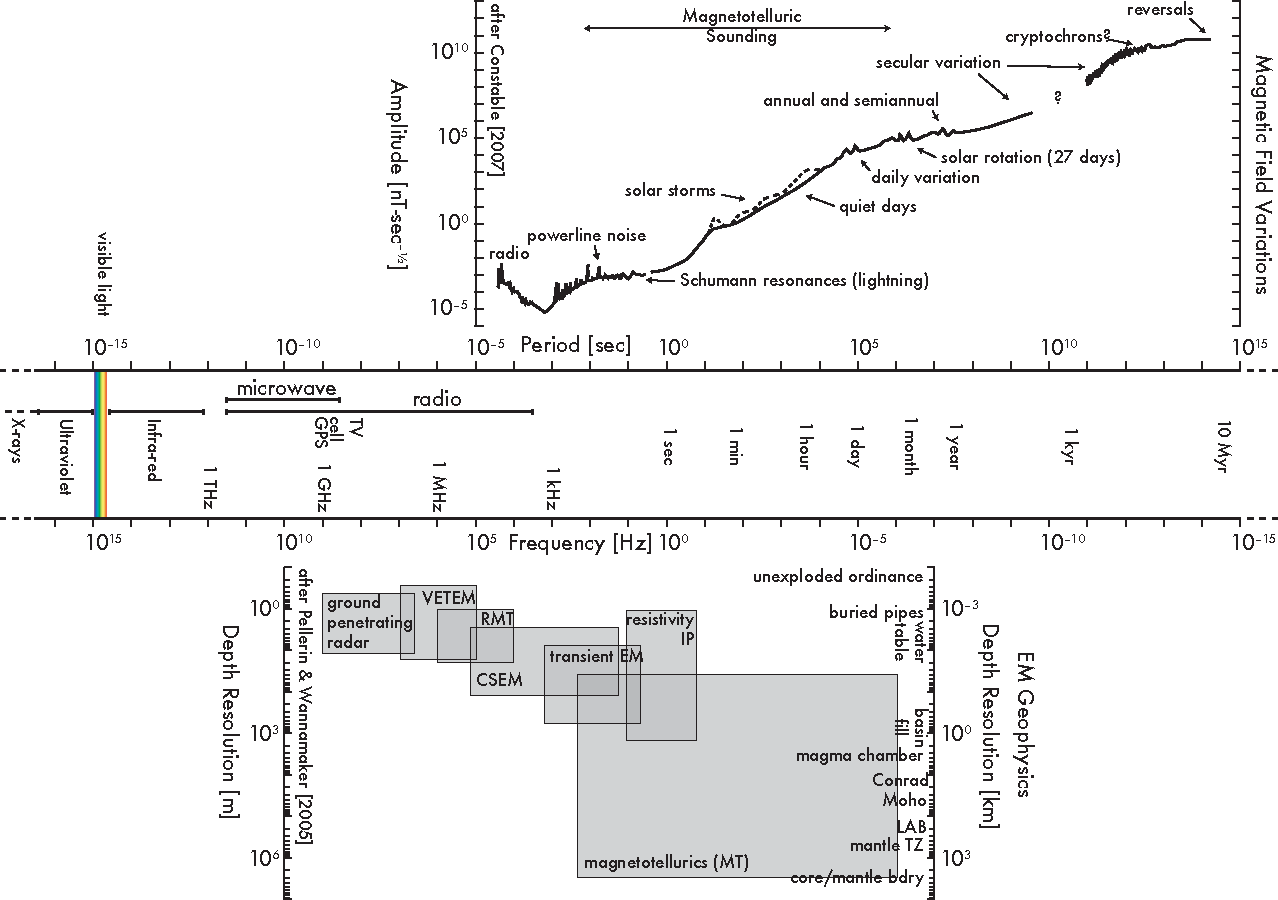
\includegraphics[angle=90]{electromagnetics/figures/EM_spectrum.pdf}
  }
  \caption{Electromagnetic spectrum utilized in geophysics.  Also shown is the
  source field for magnetotellurics (MT) and the depth resolution of each
  technique.  Abbreviations: VETEM, very-early time electromagnetics; CSEM,
  controlled-source electromagnetics; and IP, induced polarization.}
  \label{fig:spectrum}
\end{figure}

The electrical methods that you learned about in the previous few lectures are
also governed by Maxwell's equations utilizing Gauss's law of electricity which
only depends upon the electric field variations.  Now we'll be focusing on
techniques which include both the electric and magnetic field variations.  These
techniques fall into three categories:
\begin{description}
    \item[time domain,] techniques in which an applied electric field (by us)
    creates a time varying magnetic field;
    \item[frequency domain,] techniques in which time varying electric and
    magnetic fields, either natural or applied, result in time varying electric
    and magnetic fields.  Processing for these techniques are done in the
    frequency domain to simplify the mathematics;
    \item[ground-penetrating radar,] high frequency EM radiation is applied to
    the subsurface.
\end{description}

\section{Ground Penetrating Radar, GPR}
We won't spend much time on ground penetrating radar because the physics is
governed by the wave equation and as a result the techniques are in many ways
the same as seismic methods.

\section{Time-Domain Electromagnetics, TEM or TDEM}
\subsection{Magnetic induction}
The magnetic flux, $\Phi_{B}$, through a loop of wire (or body of rock) is
related to the magnetic field, $B$, by
\begin{equation*}
    \dv{\Phi_{B}}{t} = \dv{}{t} \fint{S}{} \vb{B}(t) \cdot \dd{\vb{A}}.
\end{equation*}
Hence, the $\Phi_{B}$ is the temporal change in the magnetic field through a
given area.  Assuming our loop is stationary, the magnetic flux is
\begin{equation*}
    \dv{\Phi_{B}}{t} = \fint{S}{} \dv{\vb{B}}{t} \cdot \dd{\vb{A}}.
\end{equation*}
Faraday's law tells us that a changing magnetic field within a conductive media
results in an electric field,
\begin{equation}
    \dv{\Phi_{B}}{t} = 
    \dv{}{t} \fint{S}{} \vb{B} \cdot \dd{\vb{A}} =
    -\cint{C} \vb{E} \cdot \dd{\vb{\ell}}.
    \label{eq-flux}
\end{equation}

The electromotive force (EMF), $\mathcal{E}$, is an induced voltage defined as
the energy per unit charge that travels around a loop, which we get from the
Lorentz force,
\begin{equation}
    \mathcal{E} = \cint{C} (\vb{E} + \vb{v} \times \vb{B}) \cdot
        \dd{\vb{\ell}}.
    \label{eq-emf}
\end{equation}
Again the second term on the right-hand side drops out since our loop is not
moving (i.e.\ $\vb{v} = 0$).  Therefore, from Equations \ref{eq-flux} and
\ref{eq-emf} we see that the a change in the magnetic flux (field) induces in a
EMF,
\begin{equation}
    \mathcal{E} = - \dv{\Phi_{B}}{t}.
\end{equation}

In time-domain electromagnetic, we measure this induced voltage to tell us about
the properties of the subsurface of the Earth.

\subsection{Conceptual model}
We make TEM measurements by using two loops, one which initiates the change in
magnetic flux (transmitter) and one which records the Earth's response
(receiver).  The current flowing through a transmitter is rapidly shut off,
resulting in change in the magnetic flux in the subsurface.  This change if flux
generates eddy currents which oppose the change in flux and create a
secondary magnetic field (Figure~\ref{fig:induction}).  This secondary magnetic
field decays away with time with characteristics related to the physical
properties of the body.  The decay in the secondary magnetic field generates a
change in magnetic flux in the receiver loop which generates a current that is
then measured.
\begin{figure}[hbt]
  \centerline{
    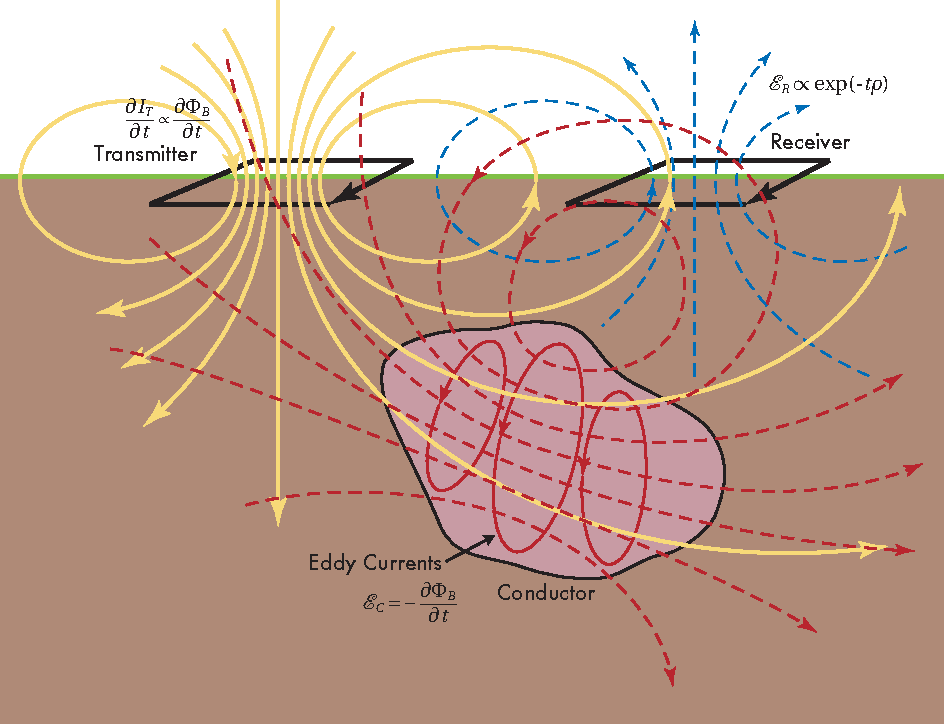
\includegraphics[]{electromagnetics/figures/induced_field.pdf}
  }
  \caption{The magnetic field of the transmitter (yellow) dissipates when it is
  switched off, inducing a current in the subsurface (solid red) generating a
  secondary magnetic field (red).  This secondary magnetic field decays
  generating a current in the receiver wire.}
  \label{fig:induction}
\end{figure}

The transmitter signal is generated by a set of alternating trapezoidal shaped
variations in current (Figure~\ref{fig:response}).  Ideally the shape would be a
square wave so that the change in flux do the transmitter is instantaneous but,
in reality, self-inductance within the loop prevents such a rapid turn-off.
Measurements are not taken during the turn-off, but are recorded during the off
time after a brief delay ($\sim\mu$s).  The response in the receiver due to the
changing Earth fields are recorded in the receiver in time gates which average
the induced voltage over a short time interval to reduce the influence of noise.
The time gates are typically recorded in a logarithmic separation in time.
\begin{figure}[hbt]
  \centerline{
    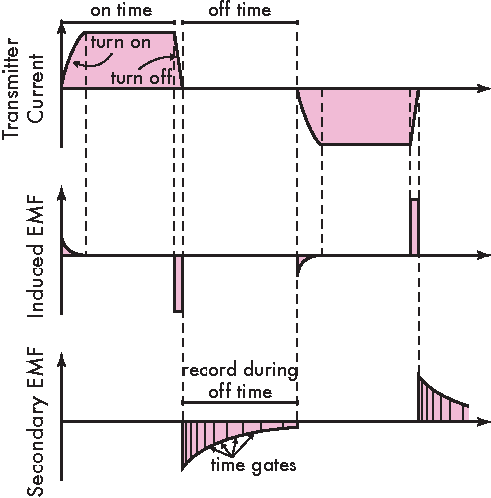
\includegraphics[]{electromagnetics/figures/induced_response.pdf}
  }
  \caption{Transient electromagnetic transmitter and receiver signals.}
  \label{fig:response}
\end{figure}

The instant the transmitter is turned off, an image current is created within
the Earth that opposes the change in the magnetic field ($t \sim 0$).  As the
induced magnetic field changes, it induces additional currents which travel
further into the Earth.  This spreading with time continues outward and
downwards with time ($t_{1}, t_{2} > 0$).  For an ideal half-space this
spreading occurs at 30$^\circ$ (Figure~\ref{fig:smoke}).  Therefore, the time
after the transmitter is turned off can be related to depth (and/or distance to
the receiver if not an in-loop configuration see below).  The field also
attenuates with time until it can no longer be resolved over ambient
(environmental and instrument) noise levels.
\begin{figure}[hbtp]
  \centerline{
    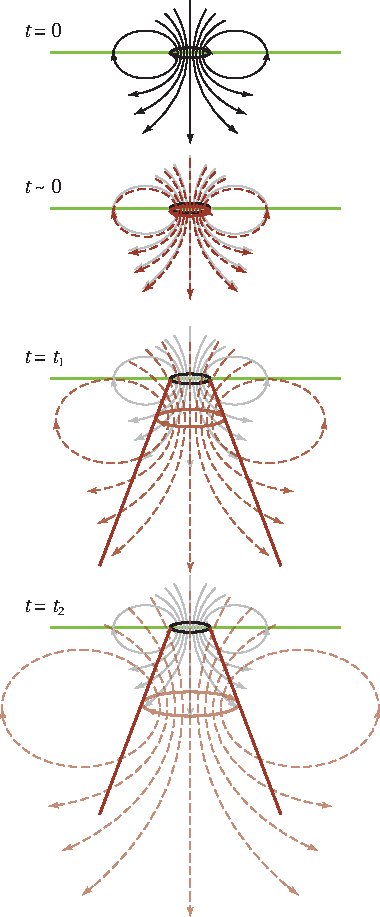
\includegraphics[]{electromagnetics/figures/smoke_rings.pdf}
  }
  \caption{Induction, spreading, and attenuation of electrical currents within
  the Earth following a change in the transmitter current.}
  \label{fig:smoke}
\end{figure}


\subsection{Circuit analogy}
The math behind electromagnetic induction in the Earth can be quite complicated
so we'll look at a simplified analogy \citep{Grant&West1965}.  The currents
induced in a conductive body can be thought of in terms of a circuit.  The
simplified circuit has an induced voltage due to the transmitter, a resistance
to the flow of current, and an inductance that resists the change in magnetic
flux through the body (Figure~\ref{fig:analogy}).  While this greatly simplifies
the actual physics, it is instructive understanding for understanding some of
the general characteristics of the true TEM method and the response to differing
properties of the subsurface.
\begin{figure}[hbtp]
  \centerline{
    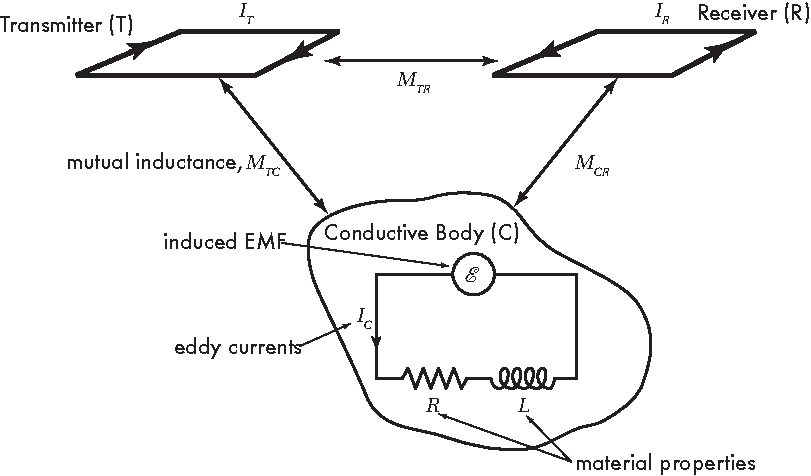
\includegraphics[]{electromagnetics/figures/circuit_analogy_bw.pdf}
  }
  \caption{A simplified view of electromagnetic induction in the Earth.}
  \label{fig:analogy}
\end{figure}

The voltage around a closed loop is zero according to Kirchoff's second law,
\begin{equation*}
    \mathcal{E} - V_{L} - V_{R} = 0.
\end{equation*}
The voltage of a resistor is given by $V_{R} = I_{\mathrm{C}}(t) R$, for an
inductor the voltage drop is $V_{L} = L \dd{I_{\mathrm{C}}(t)}\dd{t}$, where
$I_{\mathrm{C}}$ is the current flowing through the body.  The EMF coupling between
the transmitter and anomalous body is an inductive effect related to the change
in current of the transmitter.  We can write the induced voltage term as
$\mathcal{E} = - M_{\mathrm{TC}} \dv{}{t} I_{\mathrm{T}}$, where $I_{\mathrm{T}}$ is the
transmitter current. The coupling between the transmitter and conductive body
within the Earth is given by $M_{\mathrm{TC}}$ and has units of inductance.  It is
effectively a mutual inductance that depends upon the shape and size and
orientations of the transmitter loop and the conductive body as well as the
distance between the two and the conductivity of the conductive body.  Thus, we
can complete our loop,
\begin{equation}
    -M_{\mathrm{TC}} \dv{}{t}I_{\mathrm{T}}(t) - \left( L \dv{}{t}
    I_{\mathrm{C}}(t) + R I_{\mathrm{C}}(t) \right) = 0.
\end{equation}
The transmitter current is represented by a ramp function occurring over a short
time interval $\Delta t$, such that $I_{\mathrm{T}} = I_0 u(t)$ where
\begin{equation*}
    u(t) = 
    \begin{cases}
        0 & \text{if $t < 0$}, \\
        t\, \Delta t^{-1} & \text{if $0 \leq t \leq \Delta t$}, \\
        1 & \text{if $t > \Delta t$}.
    \end{cases}
\end{equation*}
\begin{figure}[hbt]
  \centerline{
    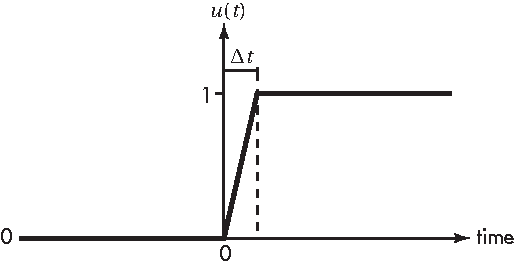
\includegraphics[]{electromagnetics/figures/u.pdf}
  }
  \caption{Normalized transmitter current, u(t). Ideally we try to make turn-on
  (-off) time, $\Delta t$, as small as possible.}
  \label{fig:u}
\end{figure}

We can rewrite the circuit voltages as
\begin{equation}
    \left( L \dv{}{t} + R \right) I_{\mathrm{C}} = 
        - M_{\mathrm{TC}} I_{0} \dv{u(t)}{t}.
    \label{eq-Ic}
\end{equation}
So lets now explore the three cases of $u(t)$.
\begin{enumerate}
    \item {\bf Before switching on the current, $t < 0$ and $u(t) = 0$.}

    This results in the trivial steady-state solution, $I_{\mathrm{C}} = 0$.

    \item {\bf As the transmitter current is turned off, $0 \leq t \leq \Delta
    t$ and $u(t) = t\, \Delta t^{-1}$.}

    The transmitter current,
    \begin{equation*}
        I_{\mathrm{T}} = I_{0} \dv{}{t} \left[ t\, \Delta t^{-1} \right] =
            I_{0}\, \Delta t^{-1},
    \end{equation*}
    when combined with Equation \ref{eq-Ic} gives
    \begin{equation*}
        \left(L \dv{}{t} + R \right) I_{\mathrm{C}}(t) 
            = - \frac{M_{\mathrm{TC}} I_0}{\Delta t}.
    \end{equation*}
    This is simply the differential equation $a_{0} \dd{y(x)}/\dd{x} + a_{1} y(x)
    = c$, with the initial condition $y(0) = y_{0}$, which has the solution $y =
    y_{0} \exp(-x a_{1}/a_{0}) + c/a_{0}$.  Using the coefficients from our ODE
    and knowing that $I_{\mathrm{C}} = 0$ at $t = 0$, we find
    \begin{equation*}
        I_{\mathrm{C}}(t) = - \frac{M_{\mathrm{TC}} I_0}{R\, \Delta t}
            \left[ 1 - \exp \left( -t \frac{R}{L} \right) \right].
    \end{equation*}
    We can simplify this expression further by using a Taylor series
    approximation for $\exp(-x) = 1 - x + \frac{1}{2}x^2 - \ldots$, which we will
    truncate after the first term.  This approximation introduces a small error
    only when $x \ll 1$, or in our case when $t \ll L/R$.  Therefore, the
    current induced in the Earth as the transmitter is turned off is
    \begin{equation}
        I_{\mathrm{C}}(t) \approx - \frac{M_{\mathrm{TC}} I_0}{L\, \Delta t} t.
    \end{equation}
    Since we will also need the initial current condition in for the third case,
    we can show that as long as our transmitter current is turned off
    sufficiently fast, $\Delta t \ll L/R$, the induced current at $t = \Delta t$
    is $I_{\mathrm{C}} = - M_{\mathrm{TC}} I_0 L^{-1}$.

    \item {\bf When the transmitter off, $t > \Delta t$ and $u(t) = 1$.}
    
    Since $\dd{u}/\dd{t} = 0$ in this case, from Equation~\ref{eq-Ic} we find
    \begin{equation*}
        \left( L \dv{}{t} + R \right) I_{\mathrm{C}} = 0.
    \end{equation*}
    This ODE is very similar to the previous one we encountered.  The solution
    of which is similar.  The solution to $a_{0} \dd{y}/\dd{x} + a_{1} y = 0$ is
    $y = k \exp (-t a_{1}/a_{0})$.  Again we input our coefficients from the
    above ODE and our final condition to the previous time interval (now our
    initial condition) to give us our estimated current in the conductive body,
    \begin{equation}
        I_{\mathrm{C}} \approx - \frac{M_{\mathrm{TC}} I_0}{L}
            \exp \left( -t \frac{R}{L} \right) .
    \end{equation}
\end{enumerate}

A similar circuit analogy may be drawn to examine the response in the receiver
loop, but I will leave that derivation as an exercise in class as well.

\begin{framed}
    {\bf Aside:} Consider the second and third cases above.  What is the induced
    current most sensitive to?  What changes as you transition from the
    early-time (case 2) to the late-time (case 3)?

    How does the value of R/L affect the rate of decay of the
    current?
\end{framed}


\subsection{TEM survey}
Transient electromagnetic measurements are conducted using two loops.  The loops
may be any shape, but typically square and nearly circular are chosen because
they simplify the math.  One loop inducing a current within the Earth
(transmitter, T) and a second which receives the Earth's response (receiver, R).
If the Earth were homogeneous or layered vertically, we would only need to
measure the vertical component.  Surveys can measure only one component of the
subsurface (usually depth), but it is not uncommon for horizontal components to
be measured as well because of their sensitivity to vertical structures.
Possible transmitter receiver pairs are shown in Figure~\ref{fig:pairs}.
\begin{figure}[hbt]
  \centerline{
    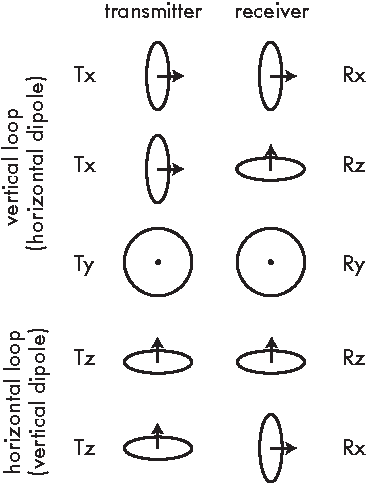
\includegraphics[]{electromagnetics/figures/tr_pairs.pdf}
  }
  \caption{Transmitter (T) and receiver (R) pair orientations.}
  \label{fig:pairs}
\end{figure}

The layout geometry may also vary again each with their own advantages and
disadvantages.  Three common variations are shown in Figure~\ref{fig:geometry}.
\begin{figure}[hbt]
  \centerline{
    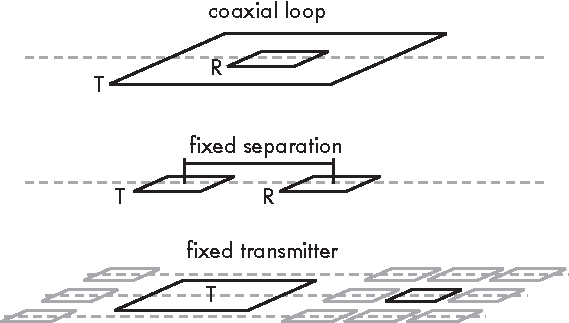
\includegraphics[]{electromagnetics/figures/tr_geometry.pdf}
  }
  \caption{Field layout geometries.}
  \label{fig:geometry}
\end{figure}
\begin{description}
    \item[Coaxial] - the receiver loop has a coincident center with the
    transmitter loop.\\
        \begin{itemize}
            \item Pros: convenient; strong signal; no blind zones 
            \item Cons: complex anomaly shape
        \end{itemize}
    \item[Fixed separation] - the transmitter and receiver loops are always the
    same distance apart.  This is the preferred method for many portable
    systems (e.g.\ aircraft, cart, hand-carry). \\
        \begin{itemize}
            \item Pros: less confusing anomaly shape
            \item Cons: weaker signals; less convenient (unless the loops are
            mounted to a movable platform)
        \end{itemize}
    \item[Fixed transmitter] - the transmitter remains in a static location
    while the receiver is placed in multiple positions. This method is often
    employed with greater depth of penetration so that a large transmitter
    moment can be employed.\\
        \begin{itemize}
            \item Pros: reduced rate of fall-off; constant source field
            \item Cons: blind zones; dependent on location of transmitter
        \end{itemize}
\end{description}

The strength of the induced voltage and receiver sensitivity are dependent upon
their magnetic moment.  If you will recall from magnetics, the magnetic moment
has units of A~m$^{2}$, which is simply a current times an area.  Therefore, for
a loop of wire with current, $I$, and area, $A$, the moment is $m = I A$.  We
can actually increase the moment by making multiple loops (or turns).  For $N$
turns of wire, the magnetic moment is $m = N I A$.

For a receiver, we typically want many turns to increase the sensitivity, but
for a transmitter, we often use only one turn and increase the current instead.
The inductance is proportional to the area and number of turns by, $L
\propto N^{2} A$.  Since the definition of inductance is related to the
magnetic flux by $\Phi_{B} = L I N^{-1}$, the greater the number of turns
the larger the flux.  The reason for a single loop transmitter is because we
want the magnetic field it generates to decay as rapidly as possible once
we switch it off.

\subsection{Sensitivity and skin depth}

The depth at which the induced magnetic field reaches a maximum is related to
the time after the current is shut off by
\begin{equation*}
    z = \left( \frac{2 t}{\sigma \mu} \right)^{1/2}.
\end{equation*}
However in reality, the depth of sensitivity is smaller by a factor of $\sim$2.

\section{Frequency-domain}
Loop-loop systems can also be used to record time data that is processed in the
frequency domain.  But I will not discuss these here.  Instead, I am going to
focus on a deeper technique.  One that is used for the study of basin structure
and hydrology, geothermal systems, and imaging the lithosphere and upper mantle. 

These solutions are for $E$ and $H$ in time and space, where $\vb{E} =
\vb{E}(x,y,z,t)$ and $\vb{H} = \vb{H}(x,y,z,t)$.

\subsection{Magnetotellurics}

\subsubsection{Helmholtz equation}
The diffusion equations in $E$ and $H$ (Equation~\ref{eq-diffusion}) are
\begin{align*}
    \nabla^2 \vb{E} = \mu \sigma \pdv{\vb{E}}{t} \\
    \nabla^2 \vb{H} = \mu \sigma \pdv{\vb{H}}{t}.
\end{align*}
The Fourier transform $\vb{E}(x,y,z,t)
\overset{\mathcal{F}}{\longleftrightarrow} \vb{E}(x,y,z,\omega)$ with $e^{i
\omega t}$ time dependence results in the Helmholtz equation,
\begin{align*}
    \nabla^2 \vb{E} + k^2 \vb{E} & = 0 \\
    \nabla^2 \vb{H} + k^2 \vb{H} & = 0, \\
\end{align*}
where $k = (1 - i) \left( \frac{\sigma \mu}{\omega} \right)$.  Note $i$ here is
referred to as the complex number, $i = (-1)^{1/2}$ (Appendix~\ref{apx:complex}
discusses complex numbers in greater detail.  The solution to the Helmholtz
equation requires additional Fourier transforms in space ($\vb{E}(x,y,z,\omega)
\overset{\mathcal{F}}{\longleftrightarrow} \vb{E}(k_x,k_y,\omega)$) to arrive at a
solution,
\begin{equation}
    \vb{E} = \underbrace{E^{(+)}(k_x,k_y,\omega) e^{i k_z z}}_{\mathrm{upgoing}}
        + \underbrace{E^{(-)}(k_x,k_y,\omega) e^{-i k_z z}}_{\mathrm{downgoing}}, 
\end{equation}
where $k_z = \left(k^2 - k_x^2 - k_y^2\right)^{1/2}$ and $E^{(+)}$ and $E^{(-)}$
are the coefficients for an upgoing and downgoing propagating fields,
respectively.  Since the $E$ and $H$ fields must vanish as $z \to \infty$ (down
into the Earth), $E^{(+)} = 0$.

\subsubsection{One-dimensional theory}
We make a number of assumptions for the 1-D case:
\begin{enumerate}
    \item the quasi-static approximation is valid; 
    \item the waves incident to the surface are planar and vertical;
    \item variations in $\mu$ and $\epsilon$ are small relative to variations in
    the conductivity and we can therefore assume the free-space values; and
    \item resistivity varies only as a function of depth, $\rho(z)$.
\end{enumerate}
The second assumption implies that $k_{x} = k_{y} = 0$ and $k_{z} = \pm k$,
where
\begin{equation}
    k = (1 - i) \sqrt{\frac{\sigma \mu_0 \omega}{2}}
\end{equation}
(Note that $k$ has real and imaginary parts).
In the 1-D solution the fields are orthogonal (i.e.\ $\vb{E} \cdot \vb{H} =
0$).  Since, $E$ and $H$ are orthogonal, we can assume $\vb{E} = E\hat{x}$ and
$\vb{H} = H\hat{y}$.  Hence we can write the fields
\begin{align}
    E_x & = E_0 e^{-(1 + i) \sqrt{\frac{\sigma \mu_0 \omega}{2}} z} \\
    H_y & = H_0 e^{-(1 + i) \sqrt{\frac{\sigma \mu_0 \omega}{2}} z}.
\end{align}

\subsubsection{Skin-depth}
Much as we have a diffusion length for TEM, we can define a skin depth as the
depth at which the fields reduce to $e^{-1}$ of their initial
magnitude.  However, the expression for our field includes the complex quantity
$k$.  We break $k$ into a real and imaginary part, $k = k_R - i k_I$, where $k_R
= \Re(k)$ and $k_I = |\Im(k)|$, respectively.  Doing so allows us to write the
electric field as
\begin{align*}
    E &= E_0 e^{-i(k_R - i k_I)z} \\
    &= E_0 e^{-k_I z} e^{-i k_R z} .
\end{align*}
Writing the electric field in the above form allows us to see that the electric
field is exponentially decreasing with depth.  Note $k_I$ is real valued with
units, length$^{-1}$.  Therefore, $k_I^{-1}$ is a characteristic depth constant,
which we call the skin depth,
\begin{align}
    \delta &= k_I^{-1} \\
    &= \left( \frac{2}{\sigma \mu_0 \omega} \right)^{1/2}.
\end{align}

\begin{framed}
The wavelength, $\lambda$, of a wave traveling through a medium is related to
the wavenumber, $k$, by
\begin{equation*}
    \lambda = 2 \pi |k|^{-1}.
\end{equation*}
The wavelength is related to the skin depth by 
\begin{equation*}
    \lambda = 2 \pi \delta ,
\end{equation*}
which allows us to write the wavelength in terms of the frequency as
\begin{equation*}
    \lambda = 2 \left( \frac{\pi \rho \tau}{\mu_0} \right)^{1/2},
\end{equation*}
recalling that $\omega = 2\pi f = 2\pi \tau^{-1}$ where $\tau$ is the period of
the wave.

The velocity of a wave can be determined by its frequency and wavelength,
\begin{equation*}
    v = \lambda f .
\end{equation*}
The phase velocity of an electromagnetic wave traveling through a medium are
related by
\begin{align*}
      v &= 2 \pi \delta \frac{\omega}{2 \pi}\\
      &= \delta \omega \\
      &= \left( \frac{2 \omega}{\sigma \mu_0} \right)^{1/2}.
\end{align*}
Note: the velocity of an electromagnetic wave is related to the conductivity of
the material (i.e., the speed of light is not constant outside of a vacuum).
\end{framed}


\subsubsection{Impedance, phase and resistivity}
{\bf Impedance} is a complex resistivity and has a frequency dependence.  We define
the impedance as
\begin{equation}
    Z = \frac{E_x(\omega)}{H_y(\omega)}.
\end{equation}
We can derive the characteristic impedance of a region then by using our
solutions to the Helmholtz equation and Faraday's law,
\begin{equation*}
    -\mu_0 \pdv{}{t} \vb{H} = \curl \vb{E}.
\end{equation*}
In the Fourier domain this equation is just
\begin{align*}
    -\mu_0 (H_y) & = \pdv{}{z} E_x \\
    -\mu_0 (H_y) & = -\frac{1}{i \omega} \pdv{}{z} \left( E_0 e^{-ikz} \right) \\
    H_y & = \frac{k}{\omega \mu_0} E_0 e^{-ikz}.
\end{align*}
Therefore,
\begin{align}
    Z & = \frac{E_{x}}{\frac{k}{\omega \mu_0}E_x} \\
    Z & = \frac{\omega \mu_0}{k}.
\end{align}

\begin{framed}
    {\bf Aside:} Free space (vacuum) also has an impedance, although $\sigma =
    0$ for free-space so we do not take the quasi-static approximation.  The
    impedance of free space is therefore defined in terms of the fundamental
    constants
    \begin{equation*}
        Z_{0} = \sqrt{\frac{\mu_0}{\epsilon_0}} \approx 376.7\; \Omega. 
    \end{equation*}
    However, do not confuse this with the resistivity of air which is on the
    order of 10$^{16}$~$\Omega$~m$^{-1}$.
\end{framed}

{\bf Resistivity} of a body is related to the conductivity by $\rho =
\sigma^{-1}$.  The goal of our magnetotelluric survey is to determine the
resistivity structure of the Earth.  We can can relate the resistivity to the
impedance above by using the definition of $k$
\begin{align*}
    Z & = \omega \mu_0 (1 + i) \left(\frac{\rho}{ 2 \omega \mu_0} \right)^{1/2} \\
      & = (1 + i) \left( \frac{\omega \mu_0 \rho}{2} \right)^{1/2}.
\end{align*}
Solving the above result for $\rho$,
\begin{equation*}
    \rho = -\frac{i}{\omega \mu_0} Z^2.
\end{equation*}
Note that this result for $\rho$ is a complex quantity.  We can choose to have a
real valued resistivity which we define as
\begin{equation*}
    \rho = \frac{1}{\omega \mu_0} | Z |^2.
\end{equation*}
For an impedance measured at the surface of the Earth, we call this the apparent
resistivity, designated by $\rho_a$, and relate it to the fields we measure at
the surface by
\begin{align*}
    \rho_a & = \frac{1}{\omega \mu_0} | Z_S |^2 \\
           & = \frac{1}{\omega \mu_0} \left| \frac{E_x}{H_y} \right|^2.
\end{align*}

{\bf Phase} is related to the imaginary part of the impedance by
\begin{equation*}
    Z = |Z| e^{i \phi}
\end{equation*}
(see Appendix~\ref{apx:complex} for a discussion of complex numbers).  We can
determine the phase by
\begin{equation*}
    \phi = \tan^{-1} \left( \frac{\Im (Z)}{\Re (Z)} \right).
\end{equation*}
While we perform our calculations in radians, we often discuss or plot the phase
in degrees.  The phase is related to the apparent resistivity by
\begin{equation*}
    \phi(\Log \omega) = \frac{\pi}{4}
        \left( 1 + \dv{(\Log \rho_a)}{(\Log \omega)} \right),
\end{equation*}
where $\Log$ is $\log_{10}$.  Therefore when the resistivity is not changing,
$\dv{(\Log \rho_a)}{(\Log \omega)} = 0$, $\phi = \pi/4$ or 45$^\circ$.


\subsubsection{Half-space model}
Now that we have defined the impedance, we would like to estimate the impedance
at the surface of the Earth, $Z_s$.  We will start with the solution for a
half-space and then build upon that to derive the solution for an arbitrary
number of horizontal layers.

The initial waves coming from above strike the Earth's surface.  Most of the
energy is reflected back into space, while a small amount is transmitted into
the Earth.  Consider three fields at the surface, the incident field, the
reflected field and the transmitted field,
\begin{align}
    \text{incident wave:} &
    \begin{cases}
        E^i_x = E^i_0 e^{-i k_0 z}, \\
        H^i_y = H^i_0 e^{-i k_0 z};
    \end{cases} \\
    \text{reflected wave:} &
    \begin{cases}
        E^r_x = E^r_0 e^{i k_0 z}, \\
        H^r_y = H^r_0 e^{i k_0 z};
    \end{cases} \\
    \text{transmitted wave:} &
    \begin{cases}
        E^t_x = E^t_1 e^{-i k_1 z}, \\
        H^t_y = H^t_1 e^{-i k_1 z}.
    \end{cases}
    \label{eq-sfield}
\end{align}
Note the sign difference for the reflected wave which denotes the field is
traveling away from the center of the Earth while the other travel towards.
Continuity of $E$ and $H$ at $z = 0$ requires
\begin{align*}
    E^i_x + E^r_x & = E^t_x, \\
    H^i_y + H^r_y & = H^t_y.
\end{align*}
Recall that impedance is given by $Z = E/H$, which allows us to write
the above equations in terms of $E$'s,
\begin{align*}
    E^i_x + E^r_x & = E^t_x, \\
    \frac{E^i_x}{Z_0} - \frac{E^r_x}{Z_0} & = \frac{E^t_x}{Z_1},
\end{align*}
where $Z_0$ and $Z_1$ are the characteristic impedances of the air and
half-space respectively.  We can solve each of these in terms of $E^i_0$,
\begin{align*}
    E^t_x = \frac{2 Z_1}{Z_0 + Z_1} E^i_x, \\
    E^r_x = \frac{Z_1 - Z_0}{Z_0 + Z_1} E^i_x.
\end{align*}
The impedance ratios above are called the transmission and reflection
coefficients, respectively.

The surface impedance is defined in terms of the total $E$ and $H$ fields at $z
= 0$, which we get from either side of Equation~\ref{eq-sfield}.  Taking then 
\begin{align*}
    Z_s & = \lim_{z \to 0} \frac{E^t_x}{H^t_y}, \\
        & = \lim_{z \to 0}
        \left[ \frac{2 Z_1}{Z_0 + Z_1} E^i_0 e^{-i k_0 z} \right]
        \left[ \left( \frac{2 Z_1}{Z_0 + Z_1} \right)
        \left( \frac{E^i_0 e^{-i k_0 z}}{Z_1} \right) \right]^{-1} \\
        & = \left[ \frac{2 Z_1}{Z_0 + Z_1} \right]
        \left[ \frac{2 Z_1}{Z_0 + Z_1} \frac{1}{Z_1} \right]^{-1} \\
        & = Z_1.
\end{align*}
Had we taken the other side of Equation~\ref{eq-sfield} we would obtain the same
result.

\subsubsection{Layered model}
For a layered model we can solve for the impedance at each layer interface very
similar to the half-space model solution by writing equations for the incident,
reflected, and transmitted waves at each interface.  The system of equations for
$N$ layers becomes $2N$.  There is another way, which allows us to circumvent
the additional equations and the method we will apply here.

The ultimate goal of this derivation is to derive a relationship for the surface
impedance as a function of frequency (angular frequency to be exact).  Why do we
just care about the surface impedance and not the impedance of each layer?  It
is because we cannot measure the impedance of each layer directly, only the
impedance at the surface.  We'll also use this relationship to develop a few
generalities that are incredibly insightful into the efficacy of the method to
provide insight about the physical properties of the Earth (specifically
conductivity/resistivity) and their dimension.

Consider a simplified model of the Earth with $N$ flat layers with differing
conductivities and thicknesses overlying a half-space with constant
conductivity.
\begin{figure}[hbt]
  \centerline{
    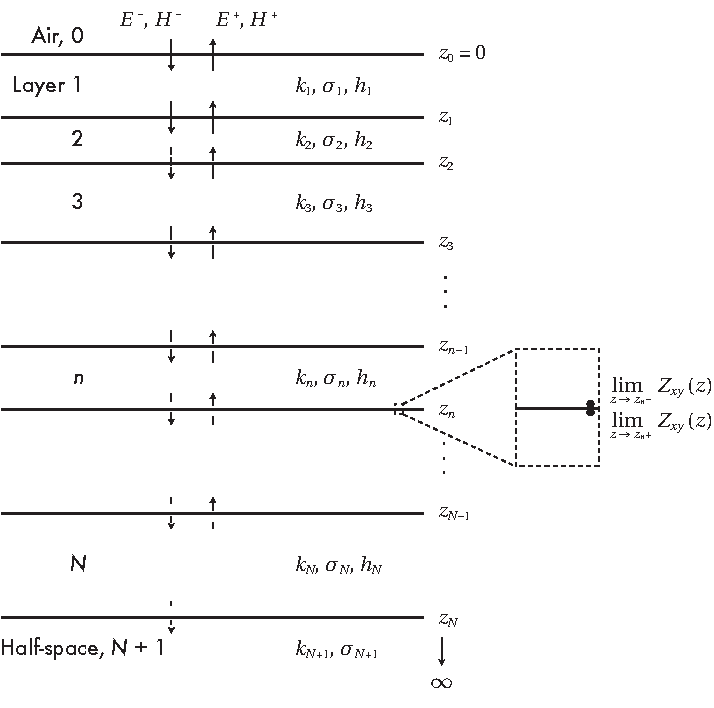
\includegraphics[]{electromagnetics/figures/EM_layers.pdf}
  }
  \caption{$N$-layered Earth over a half-space.}
  \label{fig:nlayers}
\end{figure}
For any layer, $n = [0,1,2,\cdots,N,N+1]$, there is a horizontal magnetic field
downgoing component (transmitted from above) and an upgoing component (reflected
from below),
\begin{align}
    E_{x}(z,\omega) & = E^{+}_{x,n} e^{+i k_{n} z} + E^{-}_{x,n} e^{-i k_{n} z} \\
    E_{y}(z,\omega) & = \underbrace{E^{+}_{y,n} e^{+i k_{n} z}}_{\mathrm{reflected}} +
    \underbrace{E^{-}_{y,n} e^{-i k_{n} z}}_{\mathrm{transmitted}}
    \label{eq:elayer}
\end{align}
(Figure \ref{fig:nlayers}).  For the half-space solution we also assumed that
there was only one component of the electric field.  However, for a more general
plane wave we have to consider $E$ and $H$ fields in both the $x$ and $y$
directions.  Recall in the frequency domain $\curl \vb{E} = i \omega \mu_0
\vb{H}.$  If we write this in the determinant notation (see
Appendix~\ref{apx:vcalc})
\begin{equation*}
    \curl \vb{E} (z,\omega) =
    \begin{vmatrix}
        \hat{x} & \hat{y} & \hat{z} \\
        0 & 0 & \pdv{}{z} \\
        E_{x} & E_{y} & 0
    \end{vmatrix}
    = i \omega \mu_0 (H_x \hat{x} + H_y \hat{y}),
\end{equation*}
note only derivatives in the $z$ direction are necessary because our field is
vertically incident and therefore the derivatives in the $x$ and $y$ dimensions
cancel.  Now performing the curl we find
\begin{align*}
    H_x & = -\frac{1}{i \omega \mu_0} \dv{E_y}{x} \\
    H_y & = \frac{1}{i \omega \mu_0} \dv{E_x}{y}.
\end{align*}
Now we take the derivative of the electric field within each layer,
\begin{align}
    H_x(z,\omega) & = - \frac{k_n}{\omega \mu_0} (E^{+}_{y,n} e^{+i k_{n} z} -
        E^{-}_{y,n} e^{-i k_{n} z}) \\
    H_y(z,\omega) & = \frac{k_n}{\omega \mu_0} (E^{+}_{x,n} e^{+i k_{n} z} -
        E^{-}_{x,n} e^{-i k_{n} z}).
    \label{eq:hlayer}
\end{align}
Previously, we defined the characteristic impedance of a layer as the ratio of
the electric to the magnetic fields (i.e.\ $Z = E/H$).  Because we have field
components in two orthogonal directions we can define two components of the
impedance,
\begin{align*}
    Z_{xy}(z,\omega) & = \frac{E_{x}(z,\omega)}{H_{y}(z,\omega)} \\
    Z_{yx}(z,\omega) & = -\frac{E_{y}(z,\omega)}{H_{x}(z,\omega)}.
\end{align*}
Inputting our results for the fields (Equations \ref{eq:elayer} and
\ref{eq:hlayer}) we find
\begin{equation*}
    Z_{xy}(z,\omega) = \frac{\omega \mu_0}{k_n}
        \frac{E^{+}_{x,n} e^{+i k_{n} z} + E^{-}_{x,n} e^{-i k_{n} z}}
        {E^{+}_{x,n} e^{+i k_{n} z} - E^{-}_{x,n} e^{-i k_{n} z}}.
\end{equation*}

In order to simplify our problem somewhat we are going to make two substitutions
that allow us to reduce our system of equations to a single unknown per layer
related to the ratio of the upgoing and downgoing electric fields rather each
individually.   The first will be to multiply by $(E_x^+ E_x^-)^{-1/2}/(E_x^+
E_x^-)^{-1/2}$, which is the equivalent to multiplying by 1.  This allows us to
write our impedances as the ratio of the magnitudes of the upgoing and downgoing
waves,
\begin{equation*}
    Z_{xy}(z,\omega) = \frac{\omega \mu_0}{k_n}
        \frac{(E^{+}_{x,n}/E^{-}_{x,n})^{1/2} e^{+i k_{n} z} 
            + (E^{-}_{x,n}/E^{+}_{x,n})^{1/2} e^{-i k_{n} z}}
        {(E^{+}_{x,n}/E^{-}_{x,n})^{1/2} e^{+i k_{n} z} 
            - (E^{-}_{x,n}/E^{+}_{x,n})^{1/2} e^{-i k_{n} z}}.
\end{equation*}
The next substitution allows us to put the field ratios into the exponent using
the equivalent of $e^{\log(x)} = x$,
\begin{equation*}
    (E^{+}_{x,n}/E^{-}_{x,n})^{1/2} = e^{-r_n} =
    e^{-\log[(E^{+}_{x,n}/E^{-}_{x,n})^{1/2}]}
\end{equation*}
(I am using `$\log$' to denote the natural logarithm, which is also frequently
denoted as `$\ln$').  Applying this substitution, we have
\begin{equation*}
    Z_{xy}(z,\omega) = \frac{\omega \mu_0}{k_{n}}
        \frac{e^{i k_n z - r_n} + e^{-(i k_n z - r_n)}}
        {e^{i k_n z - r_n} - e^{-(i k_n z - r_n)}},
\end{equation*}
which is simply
\begin{equation}
    Z_{xy}(z,\omega) = \frac{\omega \mu_0}{k_{n}} \coth (i k_n z - r_n),
    \label{eq:Zn}
\end{equation}
for $z_{n} < z < z_n+1$ where $\coth$ is the hyperbolic cotangent (see
Appendix~\ref{apx:hyper}).  Now we have our layer impedance in terms of single
unknown, $r_{n}$.

The horizontal components of the electric and magnetic field are continuous
across a layer interface.  Therefore, the impedance on both sides of a boundary
($z = z_n$) must also be continuous.  Since there is a discontinuity at the
boundary, we cannot simply compute the impedance at the boundary, but can
compute the result as we approach very very very closely from either side, hence
\begin{equation*}
    \lim_{z \to z_n-} Z_{xy}(z,\omega) = \lim_{z \to z_n+} Z_{xy}(z,\omega),
\end{equation*}
where $z \to z_n-$ approaches from the layer above and $z \to z_n+$ approaches
from the layer below.  Inputting the Equation~\ref{eq:Zn} from above the
interface, we have
\begin{equation*}
    \frac{\omega \mu_0}{k_{n}} \coth (i k_n z_n - r_n)
        = \lim_{z \to z_n+} Z_{xy}(z,\omega).
\end{equation*}
Solving for $r_n$, we find
\begin{equation}
    r_n = i k_n z_n - \coth^{-1} 
        \left[ \frac{k_n}{\omega \mu_0} \lim_{z \to z_n+} Z_{xy}(z) \right].
\end{equation}
Next, to find the impedance at the previous interface, $n - 1$, we will stay
within layer $n$, and approach from below and use our result for $r_n$, which
gives
\begin{equation*}
    \lim_{z \to z_{n-1}+} Z_{xy}(z,\omega) = \frac{\omega \mu_0}{k_n} 
    \coth \left\{
        i k_n z_{n-1} - 
        \left[i k_n z_{n} - 
            \coth^{-1} \left(
                \frac{k_{n}}{\omega \mu_0} \lim_{z \to z_{n}+} Z_{xy}(z,\omega)
            \right)
        \right]
    \right\}
\end{equation*}
Rearranging somewhat we find a term $i k_n (z_{n-1} - z_n)$ which is the same as
$-i k_n h_n$, where $h_n$ is the thickness of the $n$-th layer.  This allows us
to write the impedance at the top of layer $n-1$ as
\begin{equation}
    \lim_{z \to z_{n-1}+} Z_{xy}(z,\omega) = 
        \frac{\omega \mu_0}{k_n}
        \coth \left[ -i k_n h_n + \coth^{-1} \left( \frac{k_n}{\omega \mu_0}
        \lim_{z \to z_{n}+} Z_{xy} (z,\omega) \right) \right].
    \label{eq:layersoln}
\end{equation}
We can use the identity, $\coth(a + \coth^{-1} b) \equiv \tanh(a + \tanh^{-1} b)$, to
write this result in the more common form.

However, below the last layer sits a half-space (i.e.\ no lower interface) and
as a result cannot include a reflected wave traveling up through the half-space.
Hence for the half-space,
\begin{align*}
    E_x(z,\omega) & = E_{x,N+1}^- e^{-i k_{N+1} z} \\
    H_y(z,\omega) & = \frac{k_{N+1}}{\omega \mu_0} E_{x,N+1}^- e^{-i k_{N+1} z} \\
    Z_{xy}(z,\omega) = \frac{E_{x,N+1}(z,\omega)}{H_{y,N+1}(z,\omega)} & 
        = \frac{\omega \mu_0}{k_{N+1}}, \\
\end{align*}
for $z_N < z \leq \infty$.  Just as we found for the non-layered half-space case
above, the impedance at the interface with a half-space is equal to the
characteristic impedance of the half-space.

Using the above solution for impedance at the top of a layer interface
(Equation~\ref{eq:layersoln} and the impedance of the half-space, we can write a
recursive relationship to determine the impedance at the surface (our original
goal) due to all layers below,
\begin{multline}
    \lim_{z \to 0+} Z_{xy}(z,\omega) =
        \frac{\omega \mu_0}{k_1} \tanh \Biggl\{ -i k_1 h_1 
        + \tanh^{-1} \Biggl[ \frac{k_1}{k_2} \tanh \Biggl\{ -i k_2 h_2
        + \tanh^{-1} \Biggl[ \frac{k_2}{k_3} \cdots \\
        + \tanh^{-1} \Biggl[ \frac{k_{N-1}}{k_N} \tanh \Biggl\{ -i k_N h_N 
        + \tanh^{-1} \Biggl[ \frac{k_N}{k_{N+1}} \Biggr] \Biggr\} \Biggr] 
        \cdots  \Biggr] \Biggr\} \Biggr] \Biggr\}
\end{multline}

Recalling that $k_n = (1 - i)\left( \frac{\sigma_n \mu_0 \omega}{2}
\right)^{1/2}$, we can compute the surface impedance dependent only upon the
layer conductivities and thicknesses as well as the frequency, but is
independent of the magnitude of the fields.

We only derived the result for $Z_{xy}$, but if we were to derive the result for
$Z_{yx}$ as well we would find that the result is identical.  Hence for 1-D
magnetotellurics, the surface impedance is independent of our choice of
recording direction.  In general, this does not hold for the 2-D and 3-D cases.

\subsubsection{1-D generalizations}
Now that you have suffered through the derivation for the layered resistivity
case we can explore the implications of this result.  We will explore a few
simple cases that will illuminate some important aspects of magnetotelluric
sounding.

Lets consider the one-layer case, with a layer conductivity $\sigma_1$ and
thickness $h_1$ over a half-space with conductivity $\sigma_2$,
\begin{equation*}
    Z(0) = \frac{\omega \mu_0}{k_1} \tanh \Biggl[ -i k_1 h_1 
        + \tanh^{-1} \Biggl( \frac{k_1}{k_2} \Biggr) \Biggr].
\end{equation*}
Before we proceed with some special cases, lets simplify the above expression a
bit by using the identity
\begin{equation*}
    \tanh ( x + y ) = \frac{\tanh x + \tanh y}{1 + \tanh x \tanh y}.
\end{equation*}
We also know that $\tanh$ is an odd function (i.e.\ $f(-x) \equiv -f(x)$, as opposed to
an even function in which $f(-x) \equiv f(x)$).  Therefore, we can rewrite the
two layered case as
\begin{equation}
    Z(0) = \frac{\omega \mu_0}{k_1} \left( \frac{k_1 + k_2\tanh (i k_1 h_1)}
        {k_2 + k_1 \tanh (i k_1 h_1)} \right).
\end{equation}

\begin{enumerate}
    \item {\bf Thick surface layer, $h_1 \to \infty$ or $\omega \to \infty$
    ($\tau \to 0$).}

    We can show that $\tanh (i k_1 h_1) \to 1$.  This reduces the two-layered
    case to
    \begin{align*}
        Z(0) & \approx \frac{\omega \mu_0}{k_1}
            \left( \frac{k_1 + k_2} {k_2 + k_1} \right) \\
             & \approx \frac{\omega \mu_0}{k_1} = Z_1.
    \end{align*}
    Hence when the top layer is thick or the frequencies are very high such that
    the waves attenuate before reaching the half-space, the surface impedance is
    equal to the impedance of the first layer which further implies
    \begin{equation*}
        \rho_a \to \rho_1.
    \end{equation*}


    \item {\bf Thin surface layer, $h_1 \to 0$ or $\omega \to 0$ ($\tau \to
    \infty$).}

    In this case, we can show $\tan (i k_1 h_1) \to 0$ which gives for the
    two-layered solution
    \begin{align*}
        Z(0) & \approx \frac{\omega \mu_0}{k_1}
            \left( \frac{k_1} {k_2} \right) \\
             & \approx \frac{\omega \mu_0}{k_2} = Z_2
    \end{align*}
    and hence
    \begin{equation*}
        \rho_a \to \rho_2.
    \end{equation*}


    \item {\bf Thin layer approximation, $h_1$ is small relative to the
    wavelength (i.e.\ $\lambda \gg h_1$).}

    In this case $|i k_1 h_1| \lesssim 1$ which allows us to approximate $\tan
    (i k_1 h_1) \approx i k_1 h_1$.  Inputting this approximation into the two
    layer case, we can find
    \begin{equation}
        Z(0) \approx \omega \mu_0
            \left( \frac{1 + i k_2 h_1} {i k_1^2 h_1 + k_2} \right)
    \end{equation}


    \item {\bf Highly conductive basement, $\sigma_2 \to \infty$ and $\omega \to
    \infty$.}

    Recall $k = (1 - i)\left( \frac{\sigma_n \mu_0 \omega}{2} \right)^{1/2}$,
    therefore when $\sigma_1 \ll \sigma_2$, $|k_1| \ll |k_2|$ and $|k_1^2 h_1|
    \ll |k_2|$.  Employing the thin layer approximation above we find
    \begin{align*}
        Z(0) & \approx \omega \mu_0
            \left( \frac{1 + i k_2 h_1} {k_2} \right) \\
             & \approx i \omega \mu_0 h_1.
    \end{align*}
    The apparent resistivity can then be approximated by
    \begin{equation}
        \rho_a \approx \omega \mu_0 h_1^2.
    \end{equation}
    Hence when $\rho_1 \gg \rho_2$, $\rho_a$ only depends upon the thickness of
    the resistive layer above a conductive basement.  This is a somewhat
    surprising but interesting result, which implies that we are insensitive to
    the resistance of resistors.


    \item {\bf Highly resistive basement, $\rho_2 \to \infty$ and $\omega
    \to \infty$.}

    From $k$ above, $|k_1| \gg |k_2|$.  Therefore when we apply this to the thin
    layer approximation above,
    \begin{align*}
        Z(0) & \approx \frac{\omega \mu_0}{i k_1^2 h_1} \\
             & \approx \frac{1}{\sigma_1 h_1}
    \end{align*}
    and
    \begin{equation}
        \rho_a \approx \frac{1}{\omega \mu_0 (\sigma_1 h_1)^2}.
    \end{equation}
    We call the product of conductivity and thickness the conductance.  Hence
    for the case where $\rho_1 \ll \rho_2$, the $\rho_a$ only depends upon the
    conductance of the overriding layer.
\end{enumerate}


\subsubsection{Two-dimensional theory}
For the multi-dimensional case, $E$ and $H$ are no longer orthogonal and $\rho =
\rho(x,y,z)$, giving a more complex expression for the impedance.
\begin{align*}
    E_x = Z_{xx} H_x + Z_{xy} H_{y}, \\
    E_y = Z_{yx} H_x + Z_{yy} H_{y}.
\end{align*}
Now we have a bit of a problem because we only have two equations and four
unknowns.  So in order to solve for the impedance values we must record
independent sets of $E$ and $H$ fields.  We do this by dividing up our
time-series recording into independent windows.  The more windows we have, the
better statistics we have on uncertainties estimates of $Z$.

We record the $E$ and $H$ fields in two orthogonal directions which can
initially be in any orientation.  For a 2-D structure 

\section{Conductivity of Earth Materials}
You may be familiar with the resistance of a wire, which quantifies a retarding
effect on the flow of electrical charge (current).  Charges flow more readily
when resistance is low.  While resistance is useful in an electronic setting, it
is not an intrinsic physical property.  For a wire, resistance is determined by
\begin{equation}
    R = \rho \frac{L}{A},
\end{equation}
where $A$ and $L$ are the area and length of the wire, respectively, and both
geometric terms.  The physical property of which leads to the effective
resistance is the resistivity, $\rho$, and a property that we can ascribe to 
physical materials.

Electrical resistivities of Earth materials range from $<10^{-3}$ to
$>10^7$~$\Omega$~m (Figure~\ref{fig:rockrho}).  However, field observations
rarely model values $<10^{-1}$ or $>10^4$.  Why might this be the case?  Also
notice the range of these values, they vary by orders of magnitude.
\begin{figure}[hbt]
    \centering
    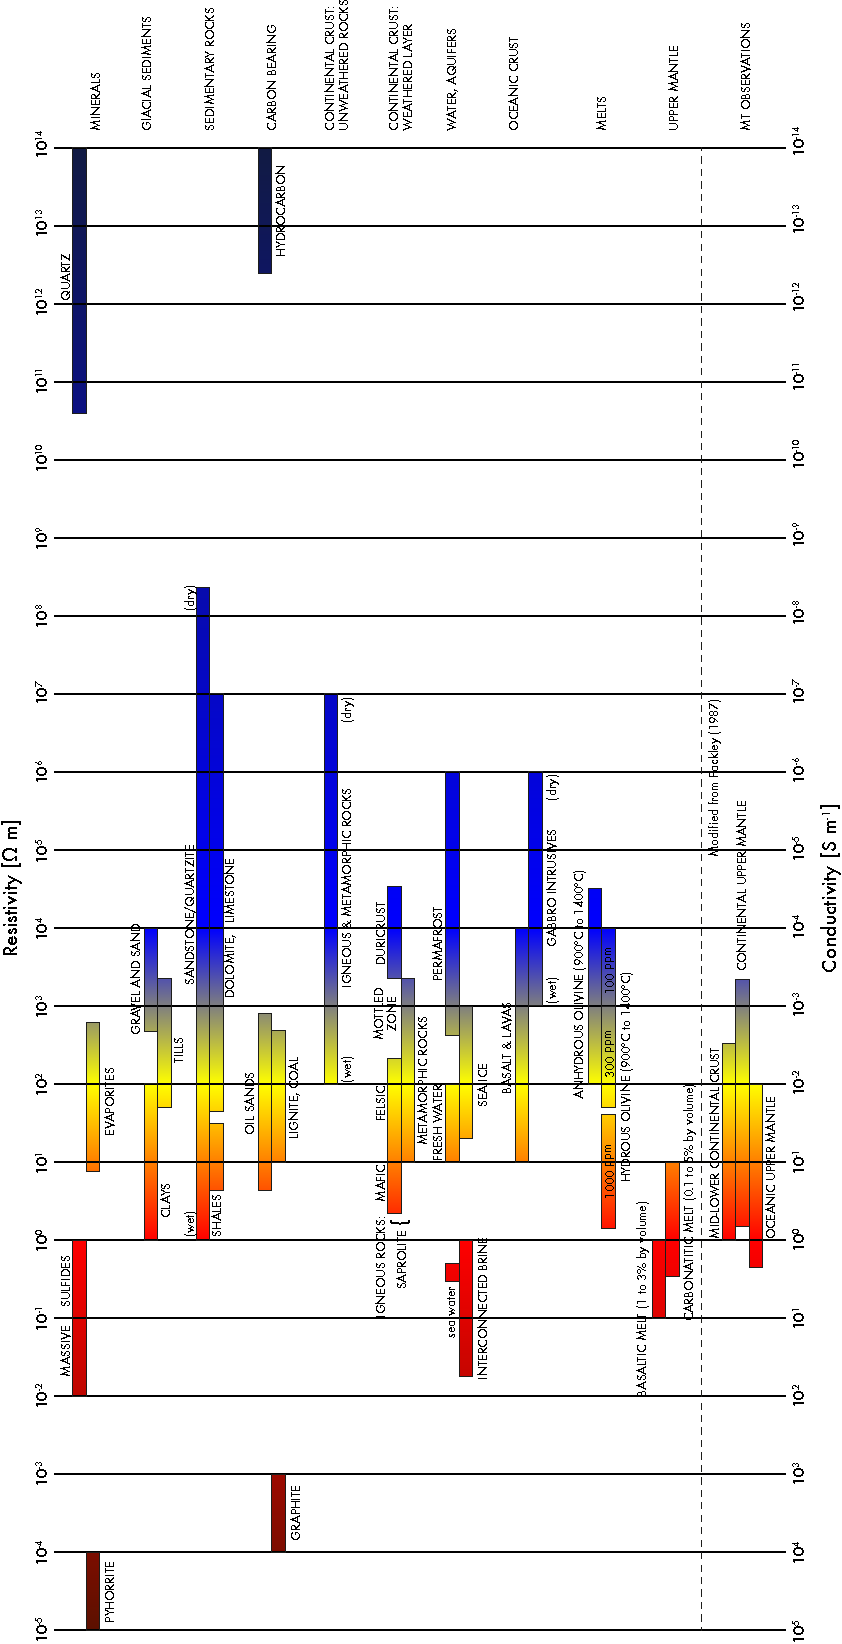
\includegraphics[height=0.95\textheight]{electromagnetics/figures/rock_resistivity.pdf}
    \caption{Resistivity of Earth materials.  Modified from \citet{Palacky1988,
    Telford_etal1990}.}
    \label{fig:rockrho}
\end{figure}

You may notice that the ranges of MT observations do not reach resistivity
values as high as those for most resistive materials or as low as most for
conductive materials.  There are few reasons for this discrepancy, (1) rocks
represent mixtures of both resistive and conductive components---conductive
minerals tend to be found in low concentrations and therefore often not well
interconnected---(2) some EM methods such as MT are insensitive to resistance
and hence never fully appreciate the high resistivities obtainable, and (3)
since many EM methods are diffusive, we model the effective conductivity over
very large volumes meaning extreme values are often smoothed.
\FloatBarrier

\subsection{Mixing Laws}
Mixing laws for conductivity are quite a bit more complex than they are for
other physical properties we have discussed.  The conductive component of
electrical conductivity can dominate conductivity at very low volume fractions,
sometimes at levels barely detectable except by chemical analysis.  There are
several mixing relations that are or have been used to estimate effective
electrical conductivity of mixtures.  We will focus on a small subset.

\subsubsection{Archie's Law}
Archie's law is technically a mixing relationship and widely used, but it has
very little sound physical basis and is instead an empirical relationship that
happens to capture some of the complexities related to the bulk resistivities of
mixtures.  Archie's law is given by
\begin{equation}
    \rho_{\mathrm{eff}} = \rho_f \phi^{-m},
\end{equation}
where $m$ is a constant, $\phi$ is the porosity, and $\rho_f$ is the
resistivity of the fluid filling the void.  For spherical particles, $m$ is
approximately 1.2; for sands, typically between 1.4 and 1.6; and for clays,
approximately 1.85, igneous rocks can have values closer to 2.6.  While Archie's
law can be a very useful relationship, it is empirical without a strong physical
basis.

Often within the petrophysical realm, the porosity term $\phi^{-m}$ is referred
to as the formation factor and used to help identify clay versus sand or other
content in borehole resistivity logs.

\subsubsection{Hashin-Shtrikman}
The Hashin-Shtrikman bounds are commonly quoted as a mixing relation for
electrical conductivity; however, the bounds often over- or under-predict the
conductivity, but that is what they are designed to do.  The bounds are
\begin{equation}
    \sigma_{\mathrm{HS}}^- = \mathcal{S}(\sigma_{\mathrm{min}}) \leq \sigma \leq
    \mathcal{S}(\sigma_{\mathrm{max}}) = \sigma_{\mathrm{HS}}^+,
\end{equation}
where $\mathcal{S}$ is defined as
\begin{equation}
    \mathcal{S}(x) =
    \Biggl( \sum_{i=1}^N \frac{\phi_i}{\sigma_i + 2x} \Biggr)^{-1} - 2x ,
\end{equation}
and $\phi_i$ is the volume fraction of the $i$-th component.

\begin{figure}[hbt]
    \centering
    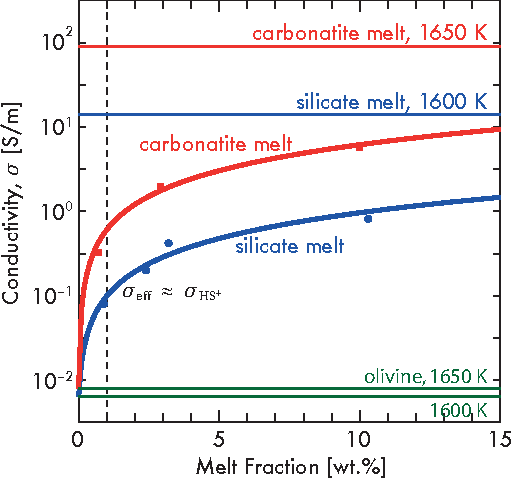
\includegraphics[]{electromagnetics/figures/melt_mixing.pdf}
    \caption{Electrical conductivity of basalt and carbonatite partial melts in
    an olivine matrix.  The results are predicted by the Hashin-Shtrikman upper
    bound.  Data from \citet{Yoshino_etal2010}.}
    \label{fig:sigmelt}
\end{figure}

\subsection{Solid Phase Conduction}
Electrical conduction occurs as charges are moved.  Generally, charges move in
response to a an applied electric or a changing magnetic field.  In solids,
moving charges requires energy, but in order for the charges to move an
activation energy (or minimum amount of energy) must be applied before the
charge will move.  The larger the activation energy, the lower the conductivity
(high resistivity).  Most charges in solid phase conduction result from the
movement of charge defects through a crystal.  Figure~\ref{fig:solidcond}
illustrates several important defects in the crystal olivine.
\begin{figure}[hbt]
    \centering
    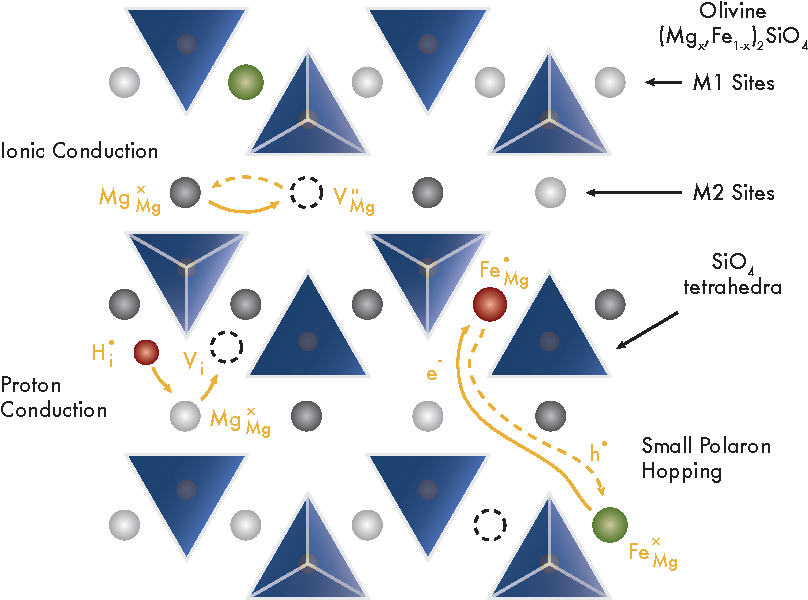
\includegraphics[]{electromagnetics/figures/conductivity_mechanism.pdf}
    \caption{Conduction mechanisms in olivine.  Conduction occurs by moving
    crystal defects through a crystal.}
    \label{fig:solidcond}
\end{figure}

The concentration of defects, $n_i$ with a crystal are temperature dependent,
\begin{equation}
    n = N \exp \left( - \frac{\Delta H_n}{k_B T} \right),
\end{equation}
where $N$ is the maximum number of defects, $\Delta H_n$ is the activation
enthalpy, $k_B$ is Boltzmann's constant, and $T$ is temperature in Kelvin.  We
describe the ability for charges to move by a parameter called mobility,
$\mu$, defined by
\begin{equation}
    \mu = m \exp \left( - \frac{\Delta H_\mu}{k_B T} \right) .
\end{equation}
where $m$ is the maximum mobility and $\Delta H_\mu$ is the activation
enthalpy.  Both the mobility and concentration can be used to determine the
electrical conductivity by
\begin{equation}
    \sigma_i = \sum_i n_i q_i \mu_i,
\end{equation}
where $i$ represents each charge defect.  For each conductivity mechanism, we
can write the electrical conductivity by a single relation,
\begin{equation}
    \sigma_i = \sigma_{0,i} \exp \left( - \frac{\Delta H_i}{k_B T} \right).
\end{equation}
The electrical conductivity due to any given defect can be expressed as a line
in $\log-\frac{1}{T}$ space,
\begin{equation}
    \log \sigma_i = \log \sigma_{0,i} - \frac{\Delta H_i}{k_B T} .
\end{equation}
This transform is convenient for plotting data as it makes it easy to observe
changes in dominant conduction mechanisms with increasing temperature
(Figure~\ref{fig:arrhenius}).  We call a $\log-\frac{1}{T}$ transform a
Arrhenius relation.
\begin{figure}[hbt]
    \centering
    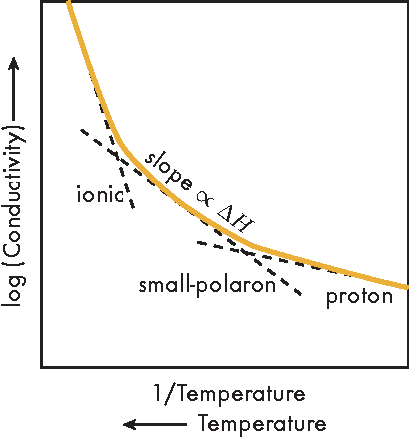
\includegraphics[]{electromagnetics/figures/arrhenius.pdf}
    \caption{Arrhenius diagram illustrating the addition the linear relationship
    between $\log$ conductivity and $1/T$.}
    \label{fig:arrhenius}
\end{figure}
The Arrhenius relationship for several mantle components is shown in
Figure~\ref{fig:sigmantle}.
\begin{figure}[hbt]
    \centering
    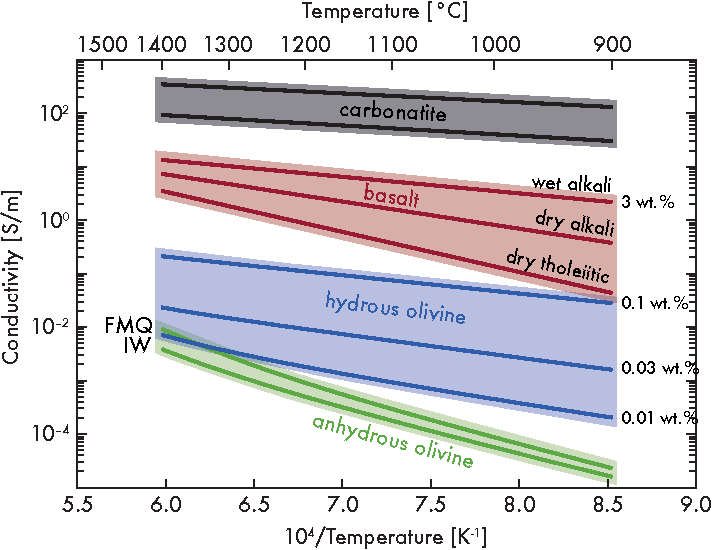
\includegraphics[]{electromagnetics/figures/mantle_conductivity.pdf}
    \caption{Arrhenius plot for conductivity of selected mantle materials.}
    \label{fig:sigmantle}
\end{figure}

\nocite{Jackson1999}
\nocite{Grant&West1965}
\nocite{Nabighian1991}

\FloatBarrier
\bibliographystyle{elsarticle-harv}
\bibliography{ref}


% Wave Equation (definitely)
% Seismology
\chapter{Seismology}\label{ch:seismology}
\section{Introduction}
\subsection{Key concepts}
\begin{itemize}
    \item What are the four types of seismic waves?  What particle motion do
    they induce?  What is the difference between a body and surface wave?

    \item What is stress? strain?  What are the differences between normal and
    shear stress/strain?  How does stress and strain relate to Hooke's law
    (material constants, e.g.\ $\sigma_{ii} = E \epsilon_{ii}$)?

    \item What is the seismic cycle?  How does it relate the magnitude to the
        frequency of earthquakes?

    \item How do the material constants relate to velocities of seismic waves?
    Why do we like Poisson's ratio so much (see first seismic practical key)?

    \item What are the three types of focal mechanisms for idealized
    earthquakes?  How do focal mechanisms relate to motion during an earthquake?
    to the stresses acting on a fault (pre-quake)?  How does it relate to
    regional tectonics?

    \item What other types of focal mechanisms are possible?  How can we use the
    focal mechanism to tell us about the source?

\end{itemize}

\subsection{Mathematical symbols and units}
\begin{table}[hbtp]
    \centering
    \caption{Definitions of symbols.}
    \label{tab:seismosym}
    \begin{tabular}{@{}cll@{}}
        \toprule
        \textbf{Symbol} &
        \textbf{Quantity} &
        \textbf{SI Unit} \\
        \midrule
        $t$             & time                          & second, \si{s} \\
        $x$, $y$, $z$   & distance                      & meter, \si{m} \\
        $\tau$          & period                        & \si{s} \\
        $f$             & frequency                     & hertz, \si{s^{-1}} \\
        $\omega$        & angular frequency ($\omega = 2 \pi f$) & \si{rad.s^{-1}} \\
        $\lambda$       & wavelength                    & \si{m} \\
        $k$             & wavenumber ($k = 2\pi \lambda^{-1}$) & \si{rad.m^{-1}} \\
        $\vb{u}$      & displacement field            & --- \\
        $F$             & force                         & newton, \si{N} \\
        $A$             & area                          & $m^2$ \\
        $\sigma$        & stress                        & pascal, $\si{Pa} = \si{N.m^{-2}}$ \\
        $\epsilon$      & strain                        & --- \\
        $\rho$          & density                       & \si{kg.m^{-3}} \\
        $\nu$           & Poisson's ratio               & --- \\
        $E$             & Young's modulus (tensile strength) & \si{Pa} \\
        $K$             & bulk modulus                  & \si{Pa} \\
        $\mu$           & shear modulus                 & \si{Pa} \\
        $V_P$, $\alpha$ & $P$-wave velocity             & \si{km.s^{-1}} \\
        $V_S$, $\beta$  & $S$-wave velocity             & \si{km.s^{-1}} \\
        \bottomrule
    \end{tabular}
\end{table}

\section{Seismology introduction}
{\it Seismology} is the study of elastic waves propagating through the Earth and
the most utilized method to study the internal structure of the planet. 

There will be two units discussed in these notes, passive source and active
source seismology.  While the underlying physical principles are the same, there
are some differences in processing and the unknowns.  {\it Passive source}
seismology is often called {\it earthquake seismology} or just seismology and
utilizes waves generated from a source with unknown location (space and time)
and characteristics (frequency range and radiation pattern).  Active source
seismology is often called {\it seismics} and utilizes a controlled source with
known location and characteristics.

The notes will start by covering the types of waves we expect to find within the
Earth and follow with the theory describing their formation and propagation.
Then we will cover a few topics of active and passive seismology.

\section{Seismic waves}
There are several types of seismic waves which propagate within the Earth, each
related to a specific type of particle motion and with differing velocities.
\begin{figure}[hbtp]
  \centerline{
    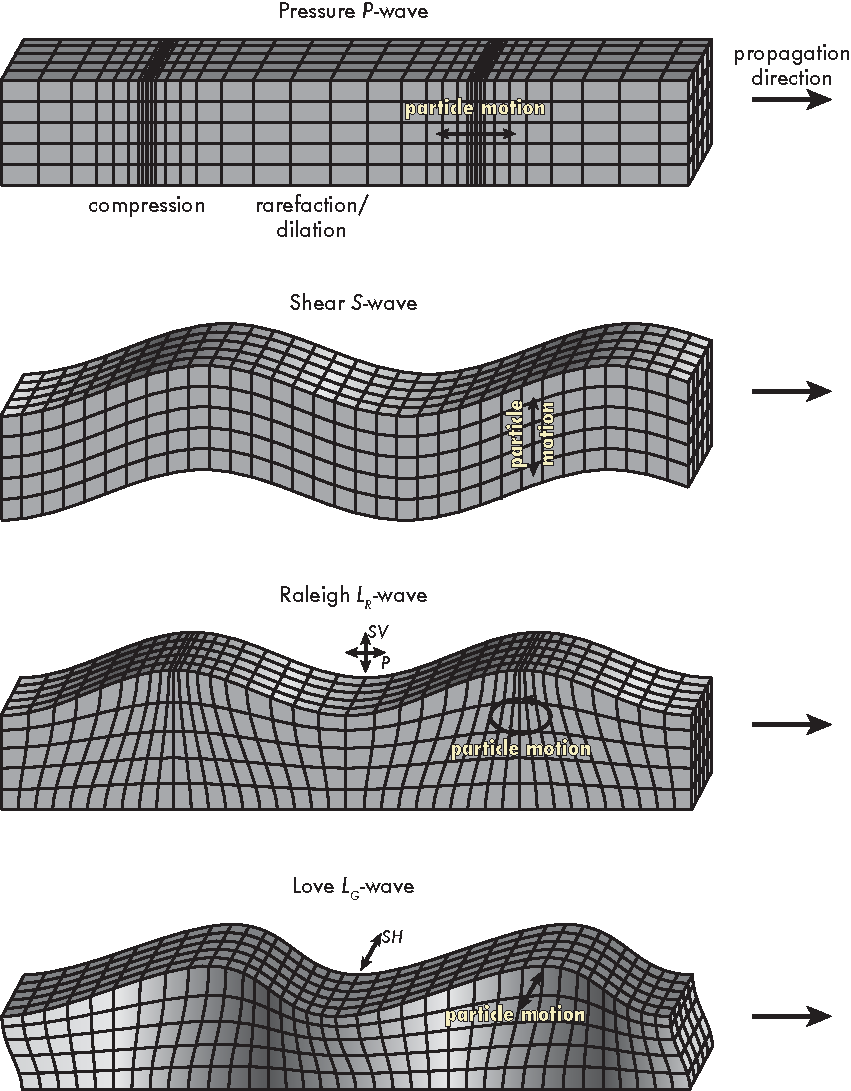
\includegraphics[]{seismology/figures/seismic_waves.pdf}
  }
  \caption{Types of seismic waves.  After Phillips (1968) and Bolt (1976).}
  \label{fig:waves}
\end{figure}


\subsection{Body waves}

\subsubsection{$P$-waves}
Also called compressional or pressure waves, $P$-waves are created by particle
motions in the direction parallel to the wave propagation.  $P$-waves can travel
through fluids such as the melts and air.  In fact the sound we hear is due to
this type of particle motion.


\subsubsection{$S$-waves}
Shear waves, $S$-waves, are created by particle motions that are orthogonal to
the direction of wave propagation.  We define two types of shear waves, $SH$ and
$SV$, to describe the $S$-waves propagating in the vertical and horizontal
direction.  $S$-waves cannot travel through fluids as fluids cannot support
shear motions, $\mu = 0$.

\subsection{Surface waves}
Surface waves are $P$- and $S$-waves that are captured at the free surface of the
Earth.  In a way, these waves are trapped.  The two types of surface waves are:
Raleigh waves, which includes both $P$- and $SV$-wave components where particle
travel in a circular motion; and Love waves, which include $SH$-wave components
where the particles move horizontally at the surface perpendicular to the
direction of propagation.

Most of the damage done due to Earthquakes is a result of surface waves.
Surface waves also travel at lower velocities than $P$-, and $S$-waves.  For
earthquakes at great distances away, it can be minutes between the arrival time
the first $P$-wave and subsequent surface waves.  Although the long delay surface
wave arrival is also related to the greater path length along the surface rather
than through the Earth.


\section{Stress and strain}
Before we can discuss wave propagation, we need to know why and how waves
propagate in the first place.  To do this, we need to understand how a material
behaves under stress.

{\it Stress} is the force applied per unit area and has the dimensions of
pressure, SI: Pa = N~m$^{2}$ (Figure~\ref{fig:ss}).

{\it Strain} represents the deformation of a body under an applied stress and
can be simply written as the change in distance between adjacent points in a
body as a function of their initial separation.  Strain is a unitless quantity
(Figure~\ref{fig:ss}).
\begin{figure}[hbtp]
  \centerline{
    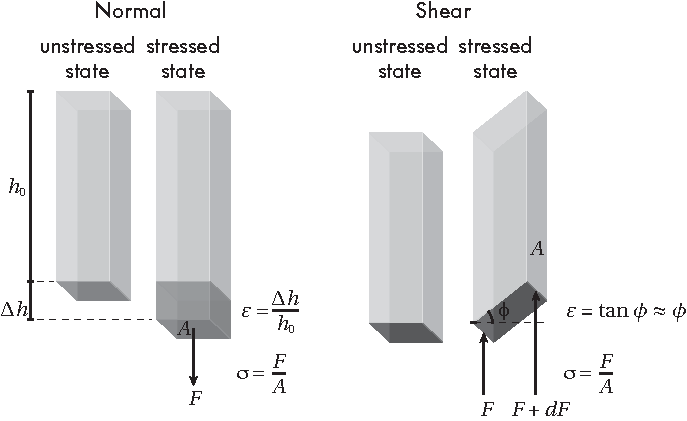
\includegraphics[]{seismology/figures/stress&strain.pdf}
  }
  \caption{Stress and strain under an applied normal and shear stress.}
  \label{fig:ss}
\end{figure}

The strain occurs as a result of applied stress.  The strain (deformation) may
be temporary, occurring under stress and restoring to the initial dimensions when
the stress is relieved, or semi-permanent to permanent, with partial or no
restoration of dimensions when stress is relieved.  When the former occurs, the
material is said to behave elastically.  When the latter occurs, the material is
said to behave plastically.  In general seismic waves propagate elastically
through the medium.

Figure~\ref{fig:hooke} shows the relationship between stress and
strain.  When the applied stress is low, the stress and strain can be related
linearly such that
\begin{equation*}
    \sigma = \frac{F}{A} \propto \frac{\Delta h}{h_0} = \epsilon.
\end{equation*}
This linear relationship is called Hooke's law and was originally used to
describe the behavior springs.  The linear proportionality breaks down as
greater stress is applied.  The deformation may still be fully restorable in
this case up to the elastic limit.  This region is called anelastic deformation.
Deformation at stresses beyond the elastic limit are said to plastically deform
and may be partially restorable.
\begin{figure}[hbtp]
  \centerline{
    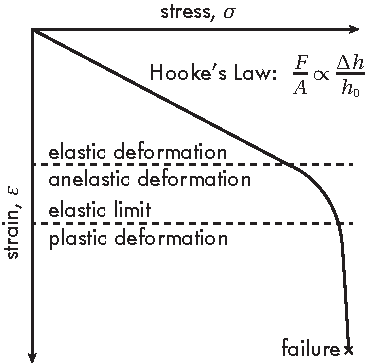
\includegraphics[]{seismology/figures/hookes_law.pdf}
  }
  \caption{The relationship between stress and strain.  Hooke's law is only
  valid in the range where strain linearly responds to stress.  After
  \citet{Lowrie1997}.}
  \label{fig:hooke}
\end{figure}


\subsection{Stress, $\sigma$}
In simplest terms, the stress is defined as
\begin{equation}
    \sigma_{ij} = \lim_{A_j \to 0} \frac{F_i}{A_j}
\end{equation}
where the subscript $i$ refers to the axis parallel to the applied force and the
subscript $j$ refers to the axis normal to the area upon which the force is
applied.

There are two types of stress: normal stress, applied force perpendicular to a
planar area (i.e.\ $i = j$); and shear stress, applied force parallel to a
planar area (i.e. $i \neq j$).  Hence for forces applied to $A_x$, we have the
three possible stress combinations
\begin{align*}
    \sigma_{xx} = & \lim_{A_x \to 0} \frac{F_x}{A_x} &\quad \text{normal stress} \\
    \sigma_{yx} = & \lim_{A_x \to 0} \frac{F_y}{A_x} &\quad \text{shear stress} \\
    \sigma_{zx} = & \lim_{A_x \to 0} \frac{F_z}{A_x} &\quad \text{shear stress}
\end{align*}
Consider some cubic volume element of some solid (infinitesimally small), there
are three axes upon which forces may be applied to each face of the cube
(Figure~\ref{fig:stress}).  Accounting for each normal and shear stress, there
are 9 possible combinations of forces applied to the faces which we can write in
matrix form as
\begin{equation*}
    \vb{\sigma} =
    \begin{bmatrix}
        \sigma_{xx} & \sigma_{xy} & \sigma_{xz} \\
        \sigma_{yx} & \sigma_{yy} & \sigma_{yz} \\
        \sigma_{zx} & \sigma_{zy} & \sigma_{zz}
    \end{bmatrix}.
\end{equation*}
This matrix is called the stress tensor.  If there is no net rotation of the
body then $\sigma_{ij} = \sigma_{ji}$ for $i \neq j$, which allows us to
simplify the matrix to six independent quantities.
\begin{figure}[hbtp]
  \centerline{
    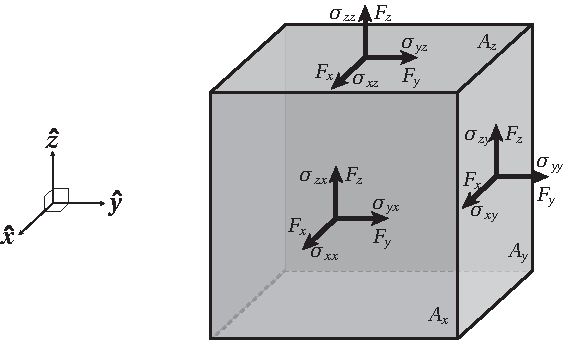
\includegraphics[]{seismology/figures/stress_element.pdf}
  }
  \caption{Stress on faces of a cube.}
  \label{fig:stress}
\end{figure}


\subsection{Strain, $\epsilon$}
Just as there are two types of stress (normal and shear), there are two types of
strain (dilation and shear).  Unlike stress which is simply the force times the
area, the strain between the dilation and shear must be treated separately.

{\bf Normal or longitudinal strain} is strain that occurs normal to the faces of
a discrete element,
\begin{align}
    \epsilon_{xx} & = \pdv{u_x}{x} \\
    \epsilon_{yy} & = \pdv{u_y}{y} \\
    \epsilon_{zz} & = \pdv{u_z}{z},
\end{align}
where $u$ is the displacement vector field describing how much each point moves
from its original position.  The normal strain forms the diagonal of a $3 \times
3$ tensor.  The total dilation represents the volume change due to the normal
strain in three dimensions,
\begin{equation}
    \phi = \epsilon_{xx} + \epsilon_{yy} + \epsilon_{zz}.
    \label{eq:dilation}
\end{equation}
We can also write this in vector notation as
\begin{equation}
    \phi = \div \vb{u}.
\end{equation}


{\bf Shear strain} is strain that occurs parallel to the faces of a discrete
element.  Under shear, the sides perpendicular to the original stress rotate by a
small angle.  Shearing along the $x$- and $y$-axis both a cause rotation of points
in the $xy$-plane.  The rotation of the points in the $xy$-plane due to a
rotation of $\delta_x$ about the $x$-axis and a rotation $\delta_y$ about the
$y$-axis (Figure~\ref{fig:shear}), can be expressed as
\begin{equation*}
    \epsilon_{xy} + \epsilon_{yx} = \delta_x + \delta_y.
\end{equation*}
The displacement due to the rotation $\delta_x$ and $\delta_y$ are
\begin{align*}
    \pdv{u_y}{x} & = \tan \delta_x \\
    \pdv{u_x}{y} & = \tan \delta_y.
\end{align*}
If $\delta_x$ and $\delta_y$ are small, we can use the small angle
approximation, $\tan \theta \approx \theta$.  Thus, we can write
\begin{equation*}
    \epsilon_{xy} + \epsilon_{yx} = \pdv{u_y}{x} + \pdv{u_x}{y} .
\end{equation*}
The shear strain is defined as half the rotation, hence
\begin{align}
    \epsilon_{xy} & = \epsilon_{yx} \\
    \epsilon_{xy} & = \frac{1}{2} \left( \pdv{u_y}{x} + \pdv{u_x}{y} \right) \\
    \epsilon_{yx} & = \frac{1}{2} \left( \pdv{u_x}{y} + \pdv{u_y}{x} \right) .
\end{align}
We can write a similar expressions for $\epsilon_{yz} = \epsilon_{zy}$ and
$\epsilon_{xz} = \epsilon_{zx}$.
\begin{figure}[hbtp]
    \centering
    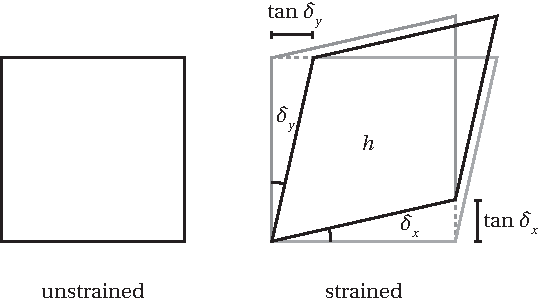
\includegraphics[]{seismology/figures/shear_strain.pdf}
    \caption{Shear strain.  As shear strain occurs in the $xy$-plane, points are rotated by and angle $\delta_x$ in the $y$ direction due to shear along the $y$-axis and rotated by an angle $\delta_y$ in the $x$ direction due to shear along the $x$-axis.  The total shear rotation is $\delta_x + \delta_y$.}
    \label{fig:shear}
\end{figure}

Now we can write the full strain tensor with all 9 components
\begin{align*}
    \vb{\epsilon} & =
    \begin{bmatrix}
        \epsilon_{xx} & \epsilon_{xy} & \epsilon_{xz} \\
        \epsilon_{yx} & \epsilon_{yy} & \epsilon_{yz} \\
        \epsilon_{zx} & \epsilon_{zy} & \epsilon_{zz}
    \end{bmatrix} \\
    & =
    \begin{bmatrix}
        \pdv{u_x}{x} &
        \frac{1}{2}\left( \pdv{u_y}{x} + \pdv{u_x}{y} \right) &
        \frac{1}{2}\left( \pdv{u_z}{x} + \pdv{u_x}{z} \right) \\
        \frac{1}{2}\left( \pdv{u_y}{x} + \pdv{u_x}{y} \right) &
        \pdv{u_y}{y} &
        \frac{1}{2}\left( \pdv{u_z}{y} + \pdv{u_y}{z} \right) \\
        \frac{1}{2}\left( \pdv{u_x}{z} + \pdv{u_z}{x} \right) &
        \frac{1}{2}\left( \pdv{u_y}{z} + \pdv{u_z}{y} \right) &
        \pdv{u_z}{z}
    \end{bmatrix}
\end{align*}

Just one additional note regarding shear.  Shear also causes a rotation of the body orthogonal to the sheared plane.  This angle is given by
\begin{align}
    \theta_{z} & = \delta_x - \delta_y \\
    & = \pdv{u_y}{x} - \pdv{u_x}{y} \\
    \theta_{y} & = \pdv{u_x}{z} - \pdv{u_z}{x} \\
    \theta_{x} & = \pdv{u_z}{y} - \pdv{u_y}{z}.
\end{align}
Note the similarity of the above equation to the curl.  We will return to this soon. 


\section{Elastic constants}

As strain occurs in one direction, a strain occurs in the two axes orthogonal to the original strained axis.  Think of this process like pulling taffy.  When you stretch the taffy in one direction, there is also a change in dimension in the other two axes.  The relationship between the strain in the original axis and the other two is a result of the material properties of the medium (Figure~\ref{fig:poisson}),
\begin{align}
    \nu & = -\frac{\epsilon_{yy}}{\epsilon_{xx}} \\
    \nu & = -\frac{\epsilon_{zz}}{\epsilon_{xx}}.
    \label{eq:poisson}
\end{align}
We call this relationship Poisson's ratio, $\nu$, and as we shall see it also relates the pressure and shear wave velocities through a medium.
\begin{figure}[hbtp]
    \centering
    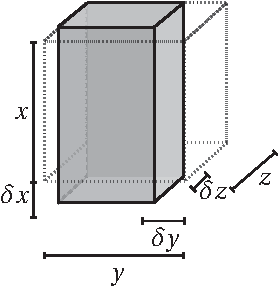
\includegraphics[]{seismology/figures/poisson.pdf}
    \caption{Dilation strain.  As strain occurs in the $x$-direction, $\epsilon_{xx} = \frac{\delta x}{x}$, a strain also occurs in the $y$- and $z$-directions, $\epsilon_{yy} = \frac{\delta y}{y}$ and $\epsilon_{zz} = \frac{\delta z}{z}$.  The strains are related by the Poisson ratio, $\epsilon_{xx} = -\nu \epsilon_{yy}$ and $\epsilon_{xx} = -\nu \epsilon_{zz}$.}
    \label{fig:poisson}
\end{figure}

As mentioned earlier, through Hooke's law, the stress and strain can be linearly related,
\begin{align}
    \sigma_{xx} & = E \epsilon_{xx} \\
    \sigma_{yy} & = E \epsilon_{yy} \\
    \sigma_{zz} & = E \epsilon_{zz}
    \label{eq:young}
\end{align}
where $E$ is a material constant called {\it Young's modulus} which is a measure of the tensile strength of a material (similar to a spring constant).  Combining Equations~\ref{eq:poisson} and \ref{eq:young}, we find that the strain in one dimension is related to stresses in all three by
\begin{align*}
    E \epsilon_{xx} & = \sigma_{xx} - \nu \sigma_{yy} - \nu \sigma_{zz} \\
    E \epsilon_{yy} & = \sigma_{yy} - \nu \sigma_{zz} - \nu \sigma_{xx} \\
    E \epsilon_{zz} & = \sigma_{zz} - \nu \sigma_{xx} - \nu \sigma_{yy}.
\end{align*}
Summing these three equations and dividing by three we have
\begin{equation*}
    E (\epsilon_{xx} + \epsilon_{yy} + \epsilon_{zz}) = 
    (1 - 2 \nu)(\sigma_{xx} + \sigma_{yy} + \sigma_{zz}) .
\end{equation*}

If the pressure is hydrostatic then $\sigma_{xx} = \sigma_{yy} = \sigma_{zz} = -P$.  Recall from Equation~\ref{eq:dilation}, $\phi = \epsilon_{xx} + \epsilon_{yy} + \epsilon_{zz}$.  Inputting these two relations into the above result, we see
\begin{equation*}
    E \phi = -3 p (1 - 2 \nu) .
\end{equation*}

We will introduce a material constant called the bulk modulus, $K$, that relates the hydrostatic pressure to the dilation,
\begin{equation}
    p = -K \phi,
\end{equation}
which we input into the previous result,
\begin{equation}
    E = 3 K (1 - 2 \nu) .
\end{equation}
The bulk modulus may also be defined in terms the Lam{\'e} constants,
$\lambda$ and $\mu$ by
\begin{equation}
    K = \lambda + \frac{2}{3} \mu ,
\end{equation}
where $\mu$ is also known as the shear modulus.

Just as we defined a proportionality constant for the dilation, we can define a {\it shear modulus} such that
\begin{align}
    \sigma_{xx} & = \mu \epsilon_{xx} \\
    \sigma_{yy} & = \mu \epsilon_{yy} \\
    \sigma_{zz} & = \mu \epsilon_{zz} .
    \label{eq:shear}
\end{align}
It can be shown that the shear modulus is related to Young's modulus and the
Poisson's ratio by
\begin{equation}
    E = 2 \mu (1 + \nu) .
\end{equation}


\section{Wave Equation}

We can write the displacement field as a combination of a scalar potential, $\phi$, related to the dilation and a vector potential, $\vb{\psi}$, related to the shear,
\begin{equation}
    \vb{u} = \grad \phi + \curl \vb{\psi} .
\end{equation}
The wave equation is defined as
\begin{equation}
    \pdv[2]{u}{t} = V^2 \nabla^2 \vb{u},
\end{equation}
where $V$ is the velocity of the wave
\begin{equation}
    V = \sqrt{\frac{E}{\rho}}.
\end{equation}

Treating each separately, we can write the wave equations for $P$-waves as
\begin{equation}
    \pdv[2]{\phi}{t} = V_P^2 \nabla^2 \phi,
\end{equation}
and for $S$-waves,
\begin{equation}
    \pdv[2]{\vb{\psi}}{t} = V_S^2 \nabla^2 \vb{\psi},
\end{equation}
where $V_P$ and $V_S$ are the $P$- and $S$-wave velocities, respectively.
The wave velocities are related to the material properties by
\begin{align}
    V_P & = \sqrt{\frac{K + \frac{4}{3} \mu}{\rho}} \\
    V_S & = \sqrt{\frac{\mu}{\rho}}.
\end{align}

We come to a peculiar solution that the wave velocities are related to the inverse of the density.  This may seem counter-intuitive and it is; however, the bulk modulus is related to the density by
\begin{equation}
    K = -V \dv{P}{V} = \rho \pdv{P}{\rho}.
\end{equation}

All of the material constants and the wave equations above have been introduced assuming a isotropic medium.  If the medium is anisotropic, then the material constants have different values in different directions.  Anisotropy is generally occurs in minerals because crystal structures are not uniform but have different shape systems.  While some minerals are isotropic (e.g.\ garnet, halite), most are not.  Major rock forming minerals such as quartz, olivine, and particularly micas have substantially different physical properties that correspond to their crystallographic axes.  As such, seismic waves may propagate at different velocities in different directions.  However, many rocks are a random aggregate of crystal orientations of various minerals which allows for isotropic approximations despite individual anisotropic components.

\section{Earthquake Seismology}
The subject of earthquake seismology is incredibly vast and one of the most useful methods by which we can study the structure and processes occurring within the Earth.  There is no way we can even cover a representative fraction of the subject in a few lectures.  Therefore, I have decided to focus on only a few aspects in some detail.  

\subsection{Seismic Cycle}
Earthquakes triggering is a complex mechanism. However, it is the same mechanisms that generate millimeter or multi-kilometer ruptures. 

During the \emph{interseismic stage}, which makes up most of the cycle, a loading (e.g. a force accumulation) occurs on asperities locating on the shallow part of the fault. This part is "locked", although some deformations affect the deeper part of the fault via a aseismic creep (figure \ref{figure_seismic_cycle}b). 

After a long period of time, the rock failure threshold $\sigma_c$ on an asperity is reached, the rock break and a slip begin at this point. This phase, the \emph{coseismic stage}, lasts few second to minutes and meters of slip on the fault "catch up" with the few mm/yr of motion that occurred during the interseismic stage (figure \ref{figure_seismic_cycle}c). This quick emission of energy generates seismic waves and unloads the asperities on a quantity called "stress drop" ($\Delta \sigma$).  When the energy released become too low to propagate the rupture, the slip stops and the asperity begin again to accumulate stresses.

Finally, a \emph{postseismic stage} occurs after the earthquake, and aftershock and transient afterslip occur for a period of years before the fault settles into its steady interseismic behavior again.
\begin{figure}[h]
    \centering
    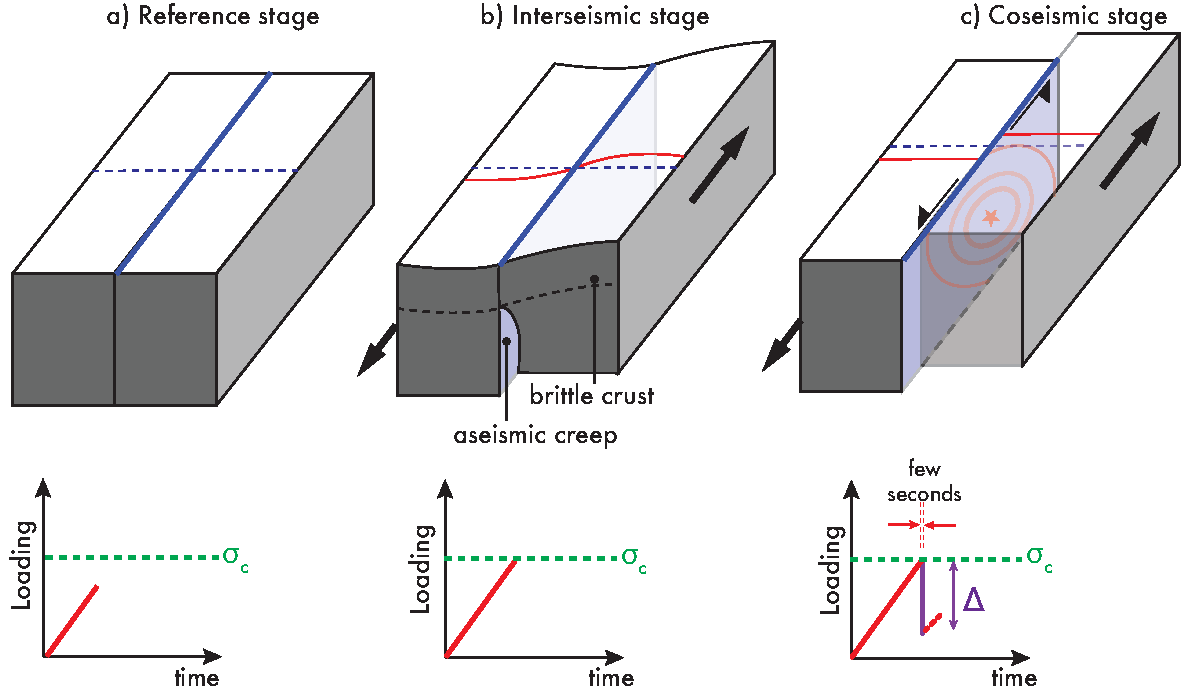
\includegraphics[trim = 5mm 180mm 0mm 0mm, clip,scale=0.6]{seismology/figures/seismic_cycle.pdf}
    \caption{From a initial stage (a), a fault accumulates loading on the locked part during the interseismic stage (b), and a slowly deformation appears on the surface. When the rock failure on the fault is reached, the coseismic stage (c) begin and the fault breaks---it's an earthquake birth.}
    \label{figure_seismic_cycle}
\end{figure}

These types of deformations can be observed by geodesy. For example, GPS stations can recorded deformation for some years for specific points on the surface, and radar interferometry (measuring precisely the displacement between two pictures of the same areas) can showed the co-seismic effect after an earthquake (Figure~\ref{figure_seismic_cycle_subduction}). 

\begin{figure}[h]
    \centering
    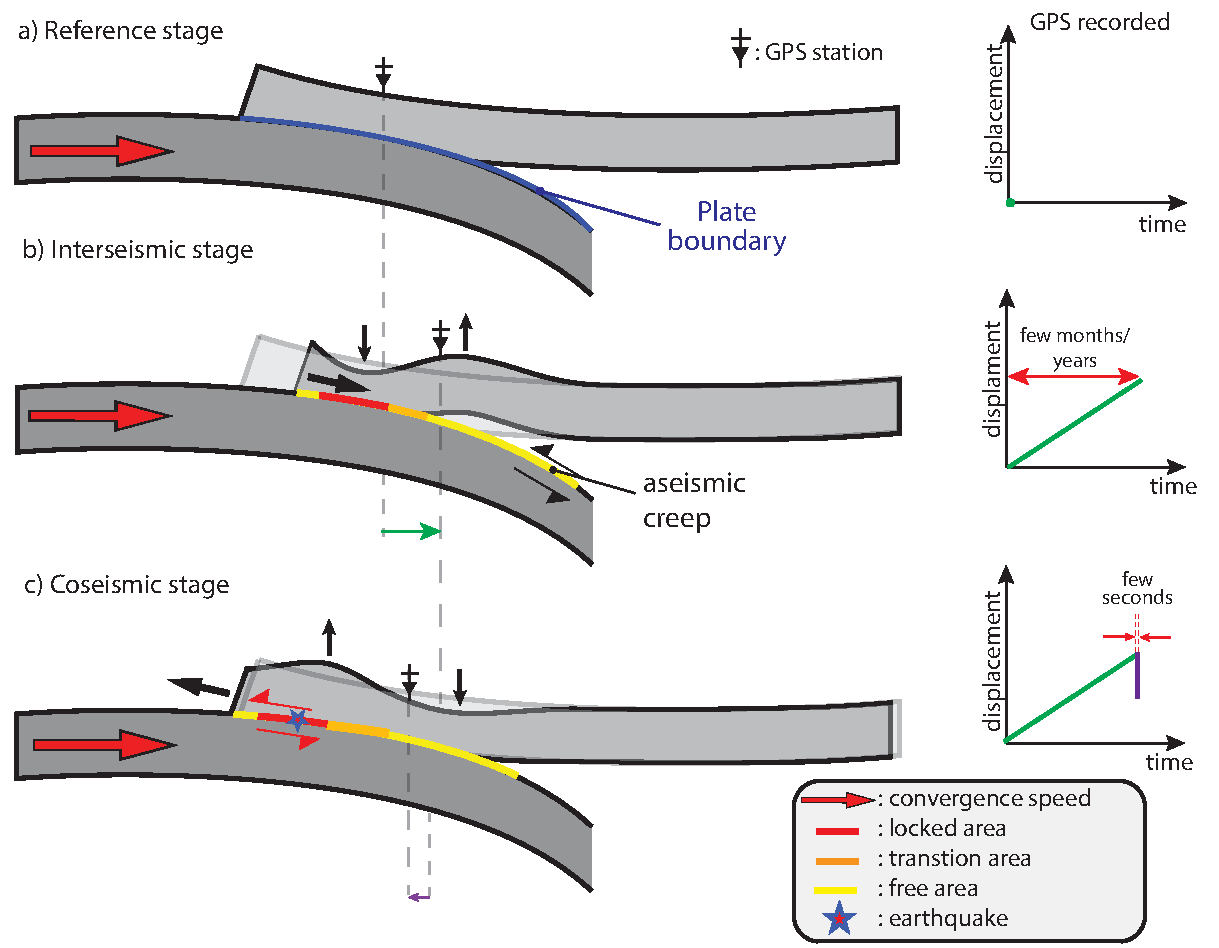
\includegraphics[trim = 5mm 120mm 0mm 0mm, clip,scale=0.5]{seismology/figures/seismic_cycle_subduction.pdf}
    \caption{Seismic cycle representation in the subduction context.  Displacements can be observed by geodetic method as GPS station. }
    \label{figure_seismic_cycle_subduction}
\end{figure}

\subsection{Magnitude}
More the energy released by earthquake is important, more earthquake will be strong. Indeed, this energy is used to break the rock and spread the rupture. A common equation to quantify this energy is the \textit{seismic moment} $M_0$:
\begin{equation}
    M_0= \mu \times  \bar{d} \times S
\end{equation}
where $\mu$ is the shear modulus (or modulus of rigidity), $\bar{d}$ is the average fault displacement on the fault with area $S$. The unit of the seismic moment is N.m (but older references express $M_0$ in \si{dyne.cm}).

For historical reasons, the most well-known measure of earthquake size is the earthquake magnitude. There are now several different types of magnitude scales but all are related to the largest amplitude that is recorded on a seismogram.  This is one of the easiest things to measure and is one reason for the continued popularity of magnitude scales.

The earliest magnitude scale and introduced by Charles Richter in 1935, is the \textit{local magnitude} $M_L$, based on the maximum amplitude $A$ (often S-waves) in micrometers recorded on standard short period (1 sec) seismometer and corrected with a standard value $A_0$ depending of the distance between source and the receiver as :
\begin{equation}
    M_L= \log_{10} (A/A_0)
\end{equation}
This magnitude is correct for earthquakes less than 1000 kilometers from the instrument measuring the earthquake.

But with time, other magnitudes types appeared. The first one is the
\textit{body-wave magnitude} $m_b$, based on the measure of the amplitude of the
P body waves generated by the earthquake, using :
\begin{equation}
    m_b= \log_{10}(A/T) + Q(D,h)
\end{equation}
where T (in second) is the period of the wave being measured, $A$ is its amplitude and $Q(D,h)$ is a correction factor that is a function of distance, $D$ (in degrees), between epicenter and station and focal depth, $h$ (in kilometers), of the earthquake

The \textit{surface wave magnitude} $M_S$ is measured using the largest
amplitude of the surface waves and its general formula is : 
\begin{equation}
    M_S= \log_{10} (A/T) + 1.66 \log_{10} (D) +3.3
\end{equation}

When initially developed, these magnitude scales were considered to be equivalent; in other words, earthquakes of all sizes were thought to radiate fixed proportions of energy at different periods. But it turns out that larger earthquakes, which have larger rupture surfaces, systematically radiate more long-period energy. Thus, for very large earthquakes, body-wave magnitudes badly underestimate true earthquake size; the maximum body-wave magnitudes are about 6.5--6.8. In fact, the surface-wave magnitudes underestimate the size of very large earthquakes; the maximum observed values are about 8.3--8.7.

To avoid these saturation problems, Kanamori in 1977 proposed the \textit{moment
magnitude} $M_w$ using the seismic moment $M_0$:
\begin{equation}
    M_w= \frac{2}{3} \log_{10} (M_0) - 6.1
\end{equation}
Now, this final formula is the most commonly magnitude used and it allows to estimate that the energy increase of factor $\times 32$  between a magnitude $M_w$ and $M_w+1$  (see table \ref{table_Seismic_Energy}).

\begin{table}[hbpt]
    \centering
    \caption{Examples of values for different historical eathquakes. (from Stein
    and Wysession 2003)}
    \label{table_Seismic_Energy}
    \begin{tabular}{ccccc}
        \toprule 
        \textbf{Earthquake} &
        \textbf{Fault Area} (km$^2$) &
        \textbf{Average} &
        \textbf{Seismic moment} &
        \textbf{Moment} \\ 
        & (length $\times$ width) & dislocation (m) & (\si{dyne.cm}), $M_0$ & magnitude,
        $M_w$ \\ 
        \midrule 
        Truckee, 1966 & 10 $\times$ 10 & 0.3  & $8.3 \times 10^{24}$ & 5.9 \\ 
        San Fernando, 1971 & 20 $\times$ 14 & 1.4  & $1.2 \times 10^{26}$ & 6.7 \\ 
        Loma Prieta, 1989 & 40 $\times$ 15 & 1.7 & $3.0 \times 10^{26}$ & 6.9 \\ 
        San Francisco, 1906 & 450 $\times$ 10& 4 & $5.4 \times 10^{27}$  & 7.8 \\ 
        Alaska, 1964 & 500 $\times$ 300 & 7 & $5.2 \times 10^{29}$ & 9.1 \\ 
        Chile, 1960 & 800 $\times$ 200 & 21 & $2.4 \times 10^{30}$ & 9.5 \\ 
        \bottomrule 
    \end{tabular} 
\end{table}

\subsection{Earthquake statistics}
\subsubsection{Relation between magnitude and frequency}
If you look at the number of earthquake per magnitude for a specific region and for a period of time,  you can observe that the number of events of low magnitudes is more important than for high magnitude. This observation was quantified by Gutenberg and Richter in the 1940s via the following relation known as the \textit{Gutenberg and Richter law} : \begin{equation} \log_{10} N=  a - b \times M \end{equation} where $N$ is the number of earthquakes with magnitude greater than $M$ occurring in a given time, $a$ depends on the number of earthquakes in the time and region sampled and the slope $b$ is generally about 1 (figure \ref{figure_GR_law}).

\begin{figure}[hbpt]
    \centering
    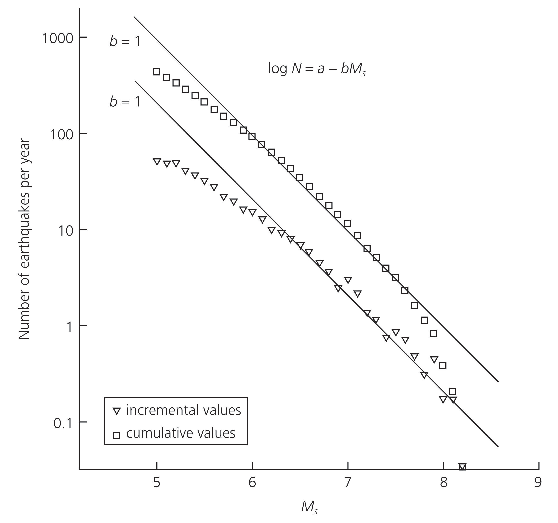
\includegraphics[trim = 0mm 0mm 0mm 4mm, clip,scale=0.9]{seismology/figures/4_7_01.pdf}
    \caption{Frequency-magnitude plot for all earthquakes with $M_S \geqslant 5.0$ during 1968-97 listed in the catalog of the National Earthquake Information Center (from Stein and Wysession 2003).}
    \label{figure_GR_law}
\end{figure}

\subsubsection{Aftershocks distribution}
After an earthquake occurrence (called mainshock), following events triggered by this earthquake, (called aftershocks) have a characteristic distribution in size and time. The largest aftershocks are usually more than a magnitude unit smaller than the mainshock, and the size distribution is agreed with the Gutenberg-Richter law, although the energy released by the aftershock is usually less than 10 $\%$ of that the mainshock.

Most of the aftershocks occur after the mainshock, and the number of events $n(t)$ is described by the relation : \begin{equation} n(t)=  \frac{K}{(t+c)^p} \end{equation} where $p$ is typically about 1, $K$ is the productivity parameter and $c$ is a constant. This law is called the Omori-Utsu law and can be observed after any earthquake (figure \ref{figure_aftershock_distribution}).
\begin{figure}[hbpt]
    \centering
    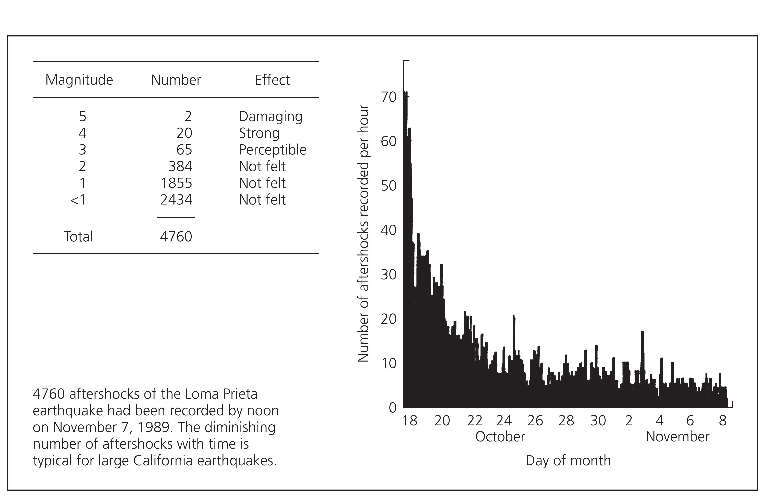
\includegraphics[trim = 2mm 2mm 2mm 8mm, clip,scale=1]{seismology/figures/4_7_08.pdf}
    \caption{Graphic showing the number and distribution aftershock in 22 days after the 1989 Loma Prieta earthquake as functions of magnitude and time (from Stein and Wysession 2003).}
    \label{figure_aftershock_distribution}
\end{figure}

It is important to know that the Earth is perpetually close to the rupture and small stress variations can trigger earthquakes.  A mainshock occurrence perturbs the stress for a specific region, and more the mainshock is important, more the perturbed region will be spread. A first perturbation mechanism is due to the dynamic stress variations produced by the seismic waves of the mainshock.  This phenomenon allows to explain aftershock occurrences in far field.  The other mechanism is called the static stress variations and corresponds to the variations due to the coseismic displacement. The coseismic displacements change the shear and normal stresses for faults present in the perturbed region by mainshock.  These variations of shear stress ($\Delta \tau_s$) and normal stress ($\Delta \sigma_n$) allows to estimate a parameter called the Coulomb stress changes ($\Delta  CFF$) with the equation:
\begin{equation}
    \Delta CFF = \Delta \tau_s + \mu' \Delta \sigma_n
\end{equation}
where $\mu'$ is the effective coefficient of friction. This value of $\Delta  CFF$ can be positive or negative and not really high (usually less than 1 bar only) but consistent observations between the region where the $\Delta  CFF$ is positive and the aftershocks locations were observed is some cases (as in 1992 Landers earthquake, in California, see figure \ref{figure_Coulomb_map}).
\begin{figure}[hbpt]
    \centering
    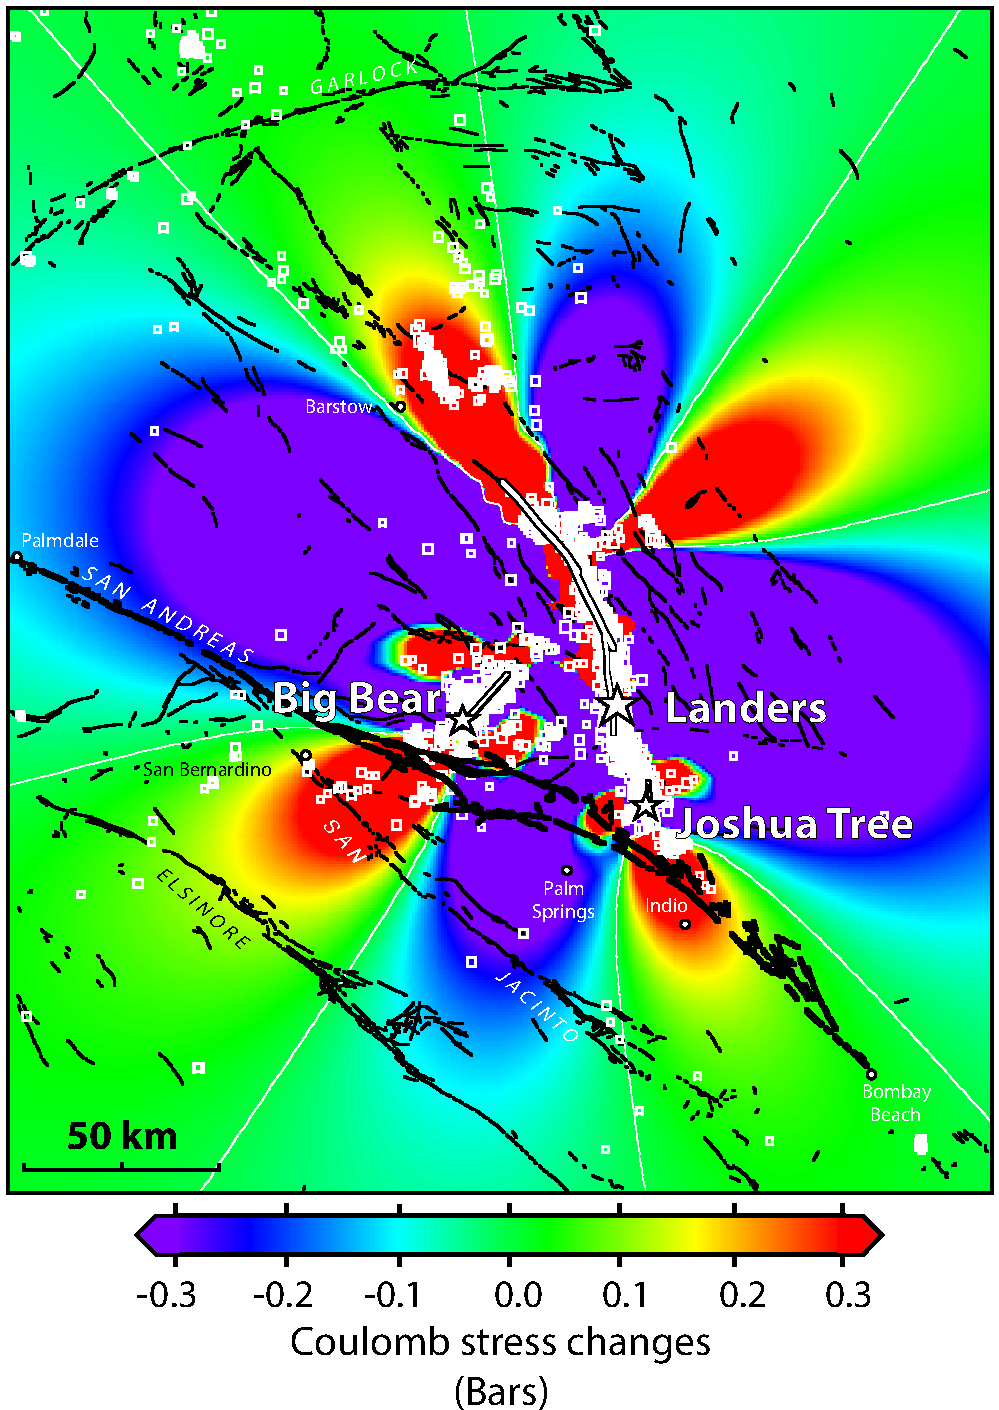
\includegraphics[trim = 25mm 10mm 23mm 20mm, clip,scale=0.5]{seismology/figures/Coulomb_Landers.pdf}
    \caption{Map of Coulomb stress changes after the occurrence of Joshua Tree,
    Landers and Big Bear earthquake. White squares indicate locations of
    aftershocks (from King et al, 1994).}
    \label{figure_Coulomb_map}
\end{figure}


\subsection{Seismograms}
The release of energy during an earthquake creates both $P$- and $S$-waves.  As
these waves travel through the earth, they reflect and refract as they interact
with changes in seismic velocities and/or acoustic impedance altering their
path, and possibly the type of wave itself.  As these waves travel through the
various layers within the Earth, they speed up and slow down in response to
these changes in velocity.  In addition to the changes in velocity the distance
the wave travels alters the time it takes for a mantle phase to reach a
seismometer.  Because rays traveling in different paths can arrive at very
similar times, we give the individual rays names based on the specific layers of
the Earth with which they interact.  An example of several phases are shown in
Figure~\ref{fig:phases}.  The naming scheme for ray paths are given in
Table~\ref{tab:phases}.
\subsection{Phases}
\begin{figure}[hbt]
    \centering
    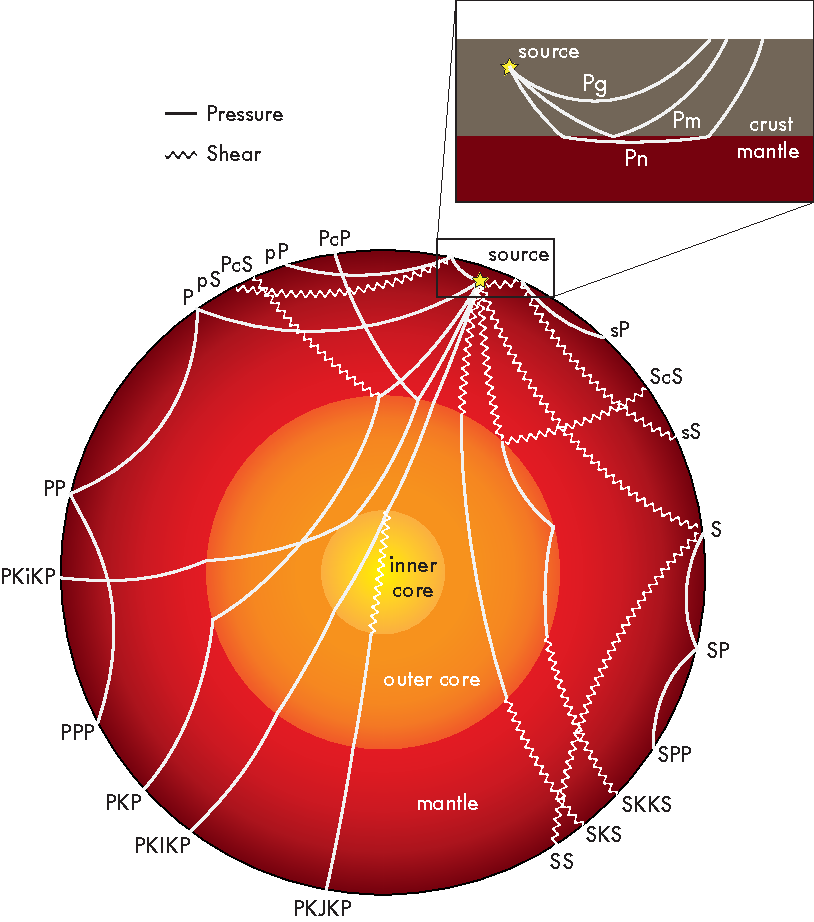
\includegraphics[]{seismology/figures/phases.pdf}
    \caption{Naming of seismic phases.  Inset shows naming scheme for selected
    crustal phases: $Pg$, internal crustal refraction; $Pm$, reflection off
    Moho; and $Pn$, critical refraction at Moho.}
    \label{fig:phases}
\end{figure}
\begin{table}[hbt]
    \centering
    \caption{Convention for seismic phases.}
    \label{tab:phases}
    \begin{tabular}{ll}
        \toprule
        \textbf{Key} & \textbf{Path} \\ 
        \midrule
        p   & short upgoing $P$-wave reflection at surface \\
        P   & $P$-wave in the mantle \\
        K   & $P$-wave in the outer core \\
        I   & $P$-wave in the inner core \\
        s   & short upgoing $S$-wave reflection at surface \\
        S   & $S$-wave in the mantle \\
        J   & $S$-wave in the inner core \\
        c   & reflection off mantle-outer core boundary \\
        i   & reflection off outer-inner core boundary \\
        \bottomrule
    \end{tabular}
\end{table}
\begin{figure}[hbt]
    \centering
    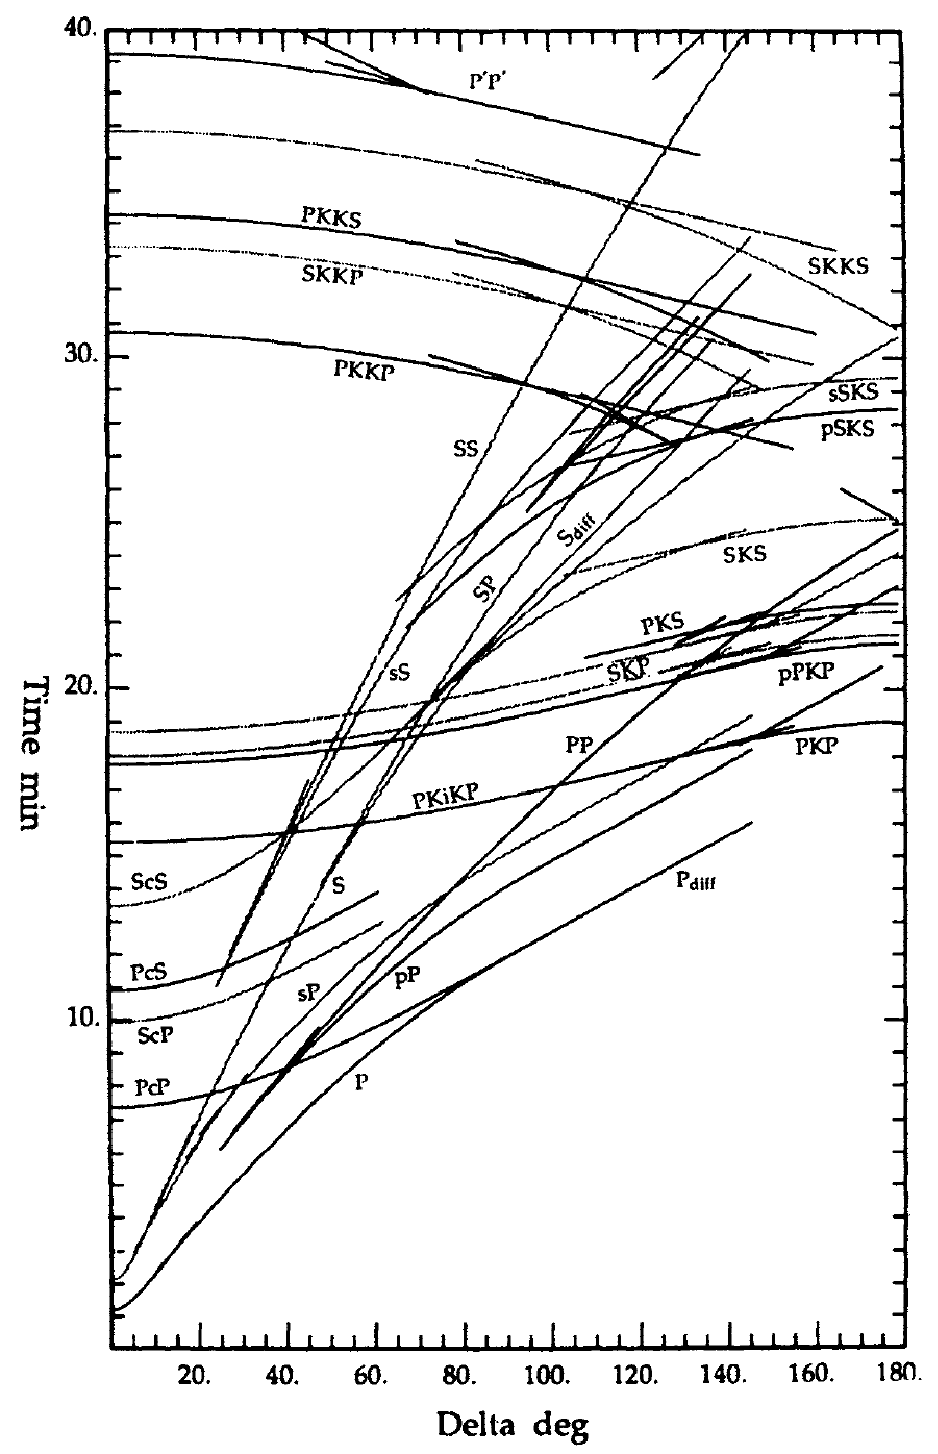
\includegraphics[]{seismology/figures/phase_travel_times.pdf}
    \caption{Estimated travel times for various phases as a function of
    epicentral difference. From \citet{Kennett&Engdahl1991}.}
    \label{fig:phasett}
\end{figure}

The combination of all these phases arriving at a single station are what build
a seismogram.  As you can imagine, the result can be quite complex
(Figure~\ref{fig:seismogram}).
\begin{figure}[hbt]
    \centering
    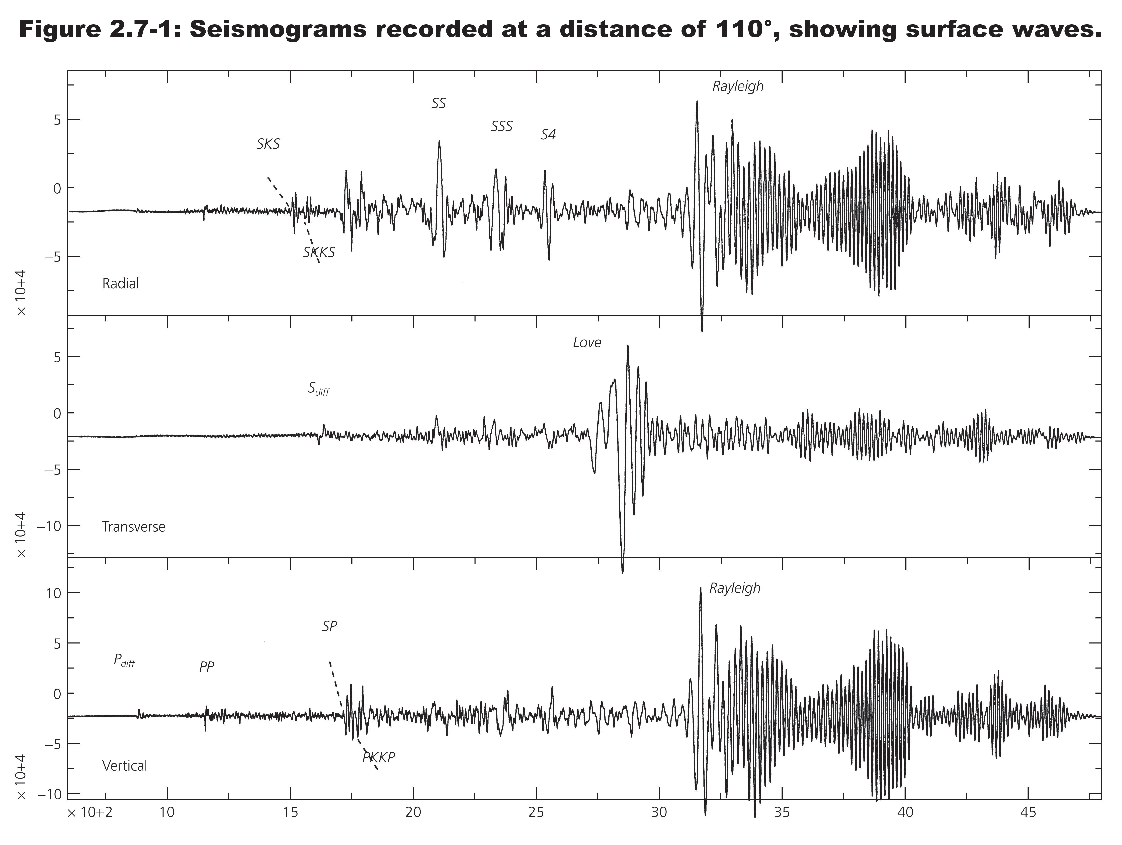
\includegraphics[width=\textwidth]{seismology/figures/seismograms.pdf}
    \caption{A seismogram with several key phases identified. From
    \citet{Stein&Wysession2003}.}
    \label{fig:seismogram}
\end{figure}


\subsection{Locating Earthquakes}
When an earthquake occurs, waves spread spherically (sort of) from the source.
The time that it takes a wave to reach an observation point (seismometer) is
proportional to the distance from the source,
\begin{equation}
    d = v t,
\end{equation}
where $d$ is the distance from the source, $t$ is the travel time of the wave
and $v$ is the velocity of the wave.  However, we typically do not know the time
of origin of the earthquake {\it a priori}.  Hence, we need some other way to
estimate distance.  Luckily, we have two types of waves with the same origin
time, which allows us to use the difference between time travels of the two
waves to estimate distance.  To do so we can write the travel time for each wave
from the source as
\begin{align}
    t_P &= \frac{d}{V_P} \\
    t_S &= \frac{d}{V_S}.
\end{align}
We can then use the above relationship to solve for the distance.
Using a relatively standard assumption for the ratio in velocities, it
can be shown that the distance from a station to the epicenter is
\begin{equation}
    d = \frac{t_S - t_P}{\sqrt{3} - 1} \bar{V}_P ,
\end{equation}
where $\bar{V}_P$ is the average $P$-wave velocity.  Note: this equation only
works for stations relatively near the source ($<$20$^\circ$) because as the
distance to the source increases the curvature of the Earth comes into play.
\FloatBarrier


\subsection{Focal Mechanisms}
A seismogram (seismic response) is a complicated observed response due to an
earthquake or from an exploration source.  Mathematically, a seismogram is
represented as
\begin{equation}
    \coreeq
    \mlbox[labelstyle={xshift=-2cm},
        linestyle={out=270,in=90, latex-}]{u(t)}{displacement (seismogram)} =
    \mlbox[labelstyle={xshift=-2cm, yshift=-1ex, below of=m\themathLableNode, below of=m\themathLableNode},
        linestyle={out=90,in=270, latex-}]
        {s(t)}{seismic source} \ast
    \mlbox[labelstyle={yshift=-2ex, below of=m\themathLableNode, below of=m\themathLableNode}]
        {G(t)}{Earth's properties} \ast
    \mlbox[
        labelstyle={xshift=2cm, yshift=-1ex, below of=m\themathLableNode, below of=m\themathLableNode},
        linestyle={out=90,in=270, latex-}]
        {Q(t)}{attenuation} \ast 
    \mlbox[]{r(t)}{seismometer/geophone response} ,
\end{equation}
where $G$ is a Green's function related to the Earth's structure including the
velocity and impedence distribution.  Note `$\ast$' here is not a multiplication
but a convolution. Obviously, this will be quite challenging to solve since we
can control $r$ and $s$ for exploration seismic studies but only $r$ for
earthquake seismology.  The attenuation $Q$ is the decrease in the amplitude of
the seismic wave as a result of viscous dissipation.

\ntextbox{Convolution}{
    A convolution describes the way in which a source wave is transformed as it
    passes through some medium, resulting in the response we measure.  The
    convolution of two time-series, $u$ and $v$, is defined by
    \[
        u(t) \ast v(t) = \int_{-\infty}^{\infty} u(\tau) v(t - \tau) \dd{\tau} .
    \]
    Since we typically use digital recordings, we can write a discrete convolution
    as
    \[
        u_i \ast v_i = \sum_{j=-\infty}^{\infty} u_{i-j} v_j ,
    \]
    where $u_i = u(t_i)$ and $v_i = v(t_i)$, respectively.  The sampling interval in
    time $\Delta t = t_{i+1} - t_i$ is constant.  The subscript $j$ represents a
    shift in integral values of $\Delta t$.  Although the definition goes from $\pm
    \infty$, we do not really perform the integration to infinity since our time
    series are finite and we assume zero magnitude on either end.  An example is
    given below in~\ref{fig:conv}.
    \vspace{4ex}

    \begin{center}
        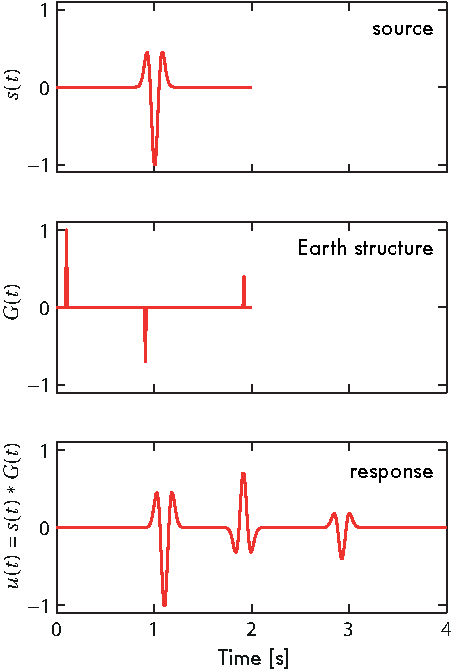
\includegraphics[]{seismology/figures/convolution.pdf}

        \textbf{Figure~\thefigure:} Convolution of two functions to produce a third.
        \label{fig:conv}
    \end{center}

    Convolutions have the following properties, $u \ast v = v \ast u$ and $u \ast (v
    \ast w) = (u \ast v) \ast w$.

    Convolutions are often made simpler by applying a Fourier transform from the
    time to frequency domain.  This has the advantage of turning our integral into a
    simple multiplication,
    \[
        u(\omega) = r(\omega) a(\omega) G(\omega) s(\omega) .
    \]
}{core}

Consider the seismic source and Earth's structure in Figure~\ref{fig:conv}. For
the moment, we will ignore the response of our seismic recorder and the
attenuation. The convolution of the source with the Earth's structure result in
a seismogram.  The sign of the Earth's structure and source affect the sign of
the convolved signal in the seismogram.  This example is quite simple resulting
in a separation of time between the arrival of each wave.  However, in reality,
the response can be significantly more complicated as the convolved response
from each interface in the Earth begins to overlap slightly for shorter period
waves or dramatically for longer period waves as shown in
Figure~\ref{fig:convw}.
\begin{figure}[htbp]
    \centering
    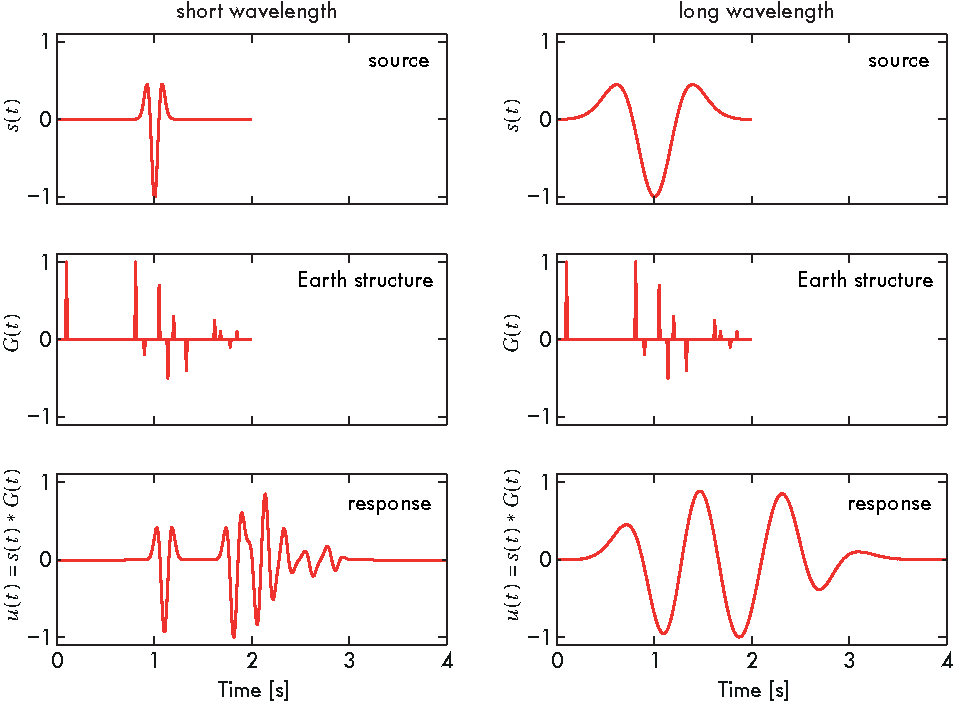
\includegraphics[]{seismology/figures/convolution_wavelength.pdf}
    \caption{Convolution of a seismic source (top row) with a Earth's structure
    (middle row) to produce a synthetic seismogram.  Note this seismogram
    ignores the effect of attenuation and reciever response for simplicity.
    Left column is a high frequency, short period wave; right column is a low
    frequency, long period wave.}
    \label{fig:convw}
\end{figure}

For an earthquake, $s(t) = M(t)$ is the moment tensor.  In earthquake
seismology, we know neither $G$ nor $M$ but wish to know both.  Focal mechanisms
are a way to graphically illustrate particular properties of $M$.

When rupture occurs along a fault, the first motion of pressure wave
(compression or rarefaction) depends upon its location relative to the fault
plane and the source location.  Imagine a point rupture on a fault plane.  In
the direction of motion of the fault slip, the first motion is a compression.
In the direction opposite of the fault slip, the first motion is a rarefaction.
Hence seismograph stations that lie within certain orientations of relative to
the earthquake's source and fault plane experience different first motions (or
polarity).
\FloatBarrier
\begin{figure}[hbtp]
    \centering
    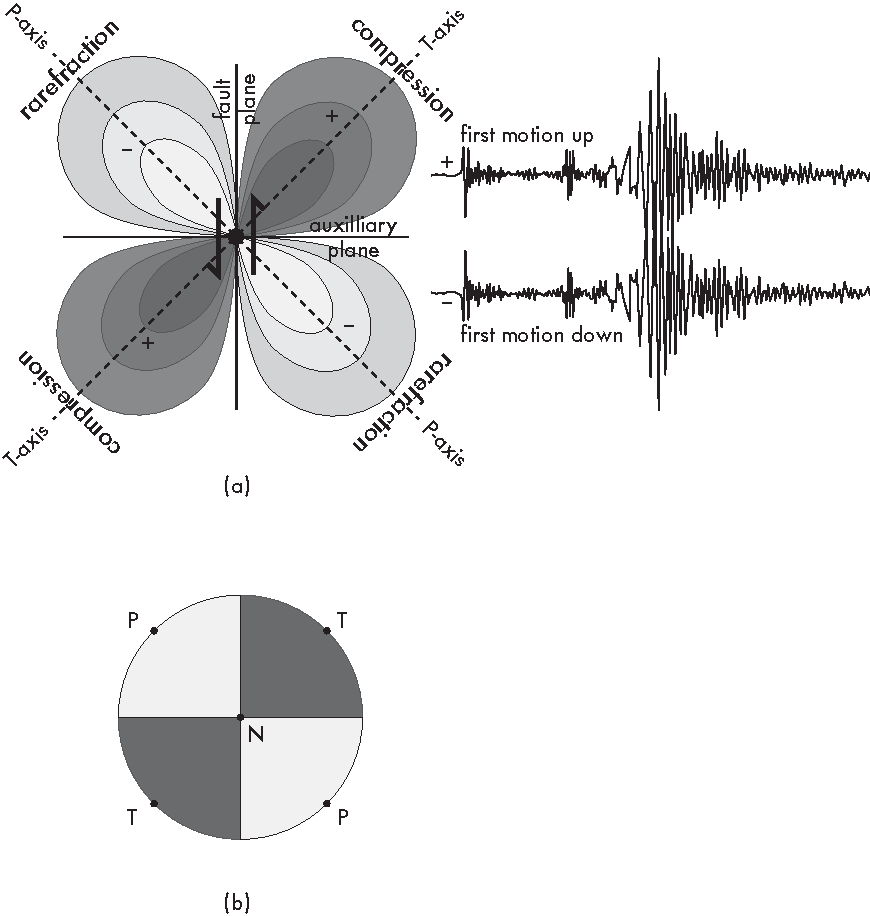
\includegraphics[]{seismology/figures/polarity.pdf}
    \caption{The $P$-wave radiation pattern from double couple mechanism (typical
    of most earthquakes) and its relation to the focal mechanism solution.
    Compression and rarefaction refer to the first motion of the elastic wave.
    The P- and T-axes are the maximum compressional and tensional axes,
    respectively, and refer to the press stress state.}
    \label{fig:polarity}
\end{figure}

Using the collective polarity observations from a global seismic network, we can
estimate the type of rupture and the orientation of the fault plane.  Graphically
we represent this with a focal mechanism (lovingly referred to as beach balls).
Mathematically, the focal mechanisms are related to the moment tensor solution
which relates to the type and orientation of the fault.  As a result the focal
mechanisms can look quite different from each other (Figure~\ref{fig:fm}). 
\begin{figure}[hbtp]
    \centering
    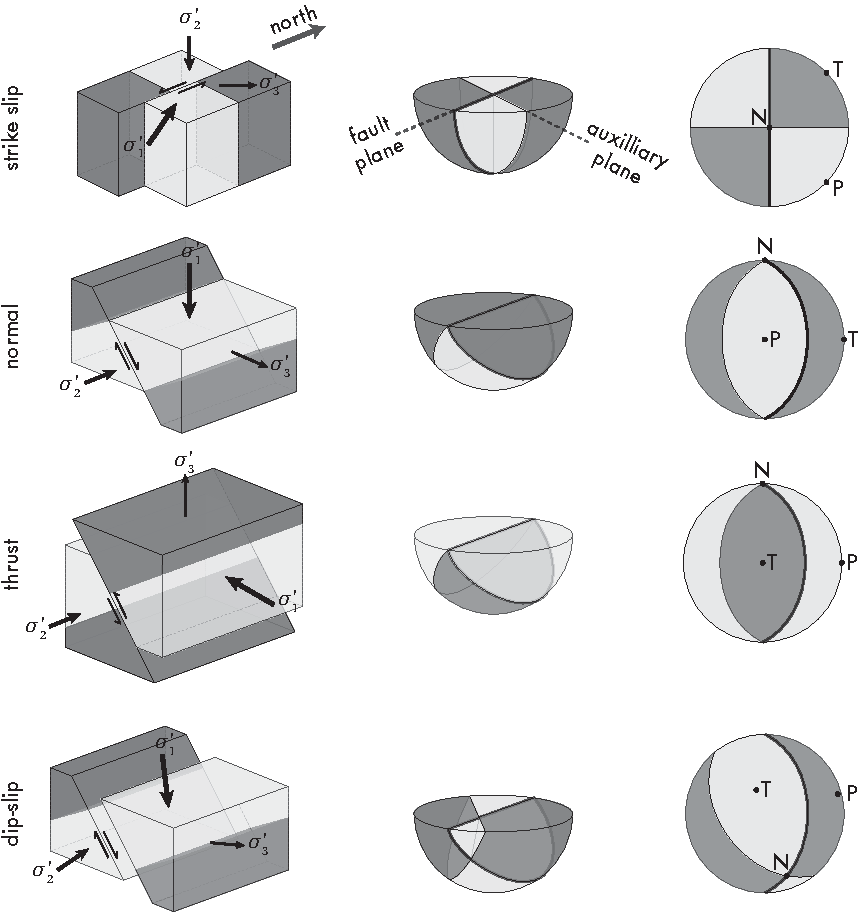
\includegraphics[]{seismology/figures/beach_balls1.pdf}
    \caption{Focal mechanisms solutions for different types of faulting and their
    relationship to maximum ($\sigma_1$) and minimum ($\sigma_3$) stresses.}
    \label{fig:fm}
\end{figure}

The center of each quadrant of the focal mechanism represents the locations of
the P- (compressional) and T- (tensional) axes of the pre-stressed state which
generated the earthquake.  Because the P- and T-axes relate to the pre-stressed
state rather than the stress during the earthquake rather than the quadrants of
first motions indicated by the color of the quadrant.  The intersection of all
four quadrants represents the neutral axis and is sometimes labeled N (not to be
confused with north).  The focal mechanisms can be used to estimate the strike
and dip of the fault as well.  Since there are four quadrants, there is a
90$^\circ$ ambiguity of the fault plane, one of which is the true fault plane
and the other we call the auxiliary plane.

Consider the case where we can decompose (rotate) our stress tensor into the
principle stresses
\begin{equation*}
    \vb{\sigma} =
    \begin{bmatrix}
        \sigma_1 & 0 & 0 \\
        0 & \sigma_2 & 0 \\
        0 & 0 & \sigma_3
    \end{bmatrix},
\end{equation*}
such that $\sigma_1 > \sigma_2 > \sigma_3$.  If we subtract the mean of the three stresses then we have the deviatoric stress that we typically care about in geoscience
\begin{equation}
    \text{maximum tension }
    \sigma_1' > \sigma_2' > \sigma_3'
    \text{maximum compression }.
\end{equation}
In the ideal case, the $\sigma_1'$ and $\sigma_3'$ stress directions would directly relate to the P- and T-axes; however, in rocks the failure planes are not oriented 45$^\circ$ to the rupture, but at an angle typically between 20$^\circ$ and 30$^\circ$.

There are a number of other sources types some of which are shown in Figure~\ref{fig:fm2}.  Not all of these source types have three stress axes as many of these solutions result from cylindrical or spherically symmetric stress patterns.
\begin{itemize}
    \item Technically the majority of an earthquake source is a double couple mechanism which has four quadrants (quadrupole).  However, because fault surfaces are not purely planar and compressible fluids often exist along fault zones the source mechanisms can be a bit more complicated.  Since we assume very little volume change, most earthquakes can by modeled by some component of a CLVD (compensated linear vector dipole) solution in addition to the double couple.

    \item Purely expansive mechanisms to identify nuclear blasts by ``rogue'' nations.  The purely contractional (implosion) mechanism may more closely represent a mine collapse (although they often appear more like crack closures).

    \item Crack opening mechanisms may be important in induced seismicity due to fracking or other fluid injection sites.  Additionally, magma injection may also appear as a crack opening mechanism.  Crack closing mechanisms may result from extraction of fluids.
\end{itemize}
\begin{figure}[hbtp]
    \centering
    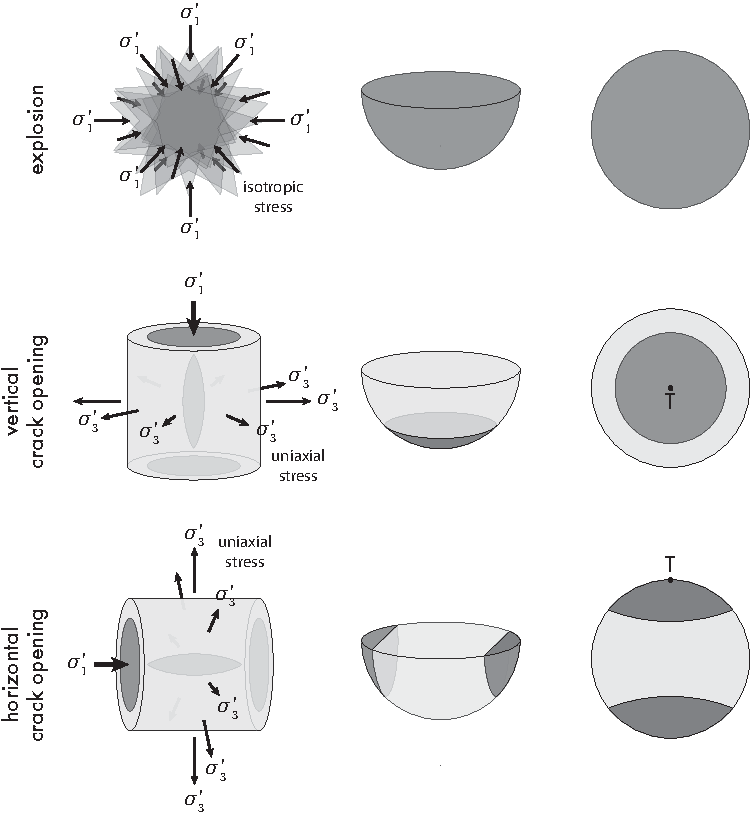
\includegraphics[]{seismology/figures/beach_balls2.pdf}
    \caption{Focal mechanisms solutions for sources other than pure end-member
    fault types.}
    \label{fig:fm2}
\end{figure}

\subsection{Focal Mechanisms construction}
An earthquake is a quick displacement on the fault plan. The focal mechanism is
a usefull tool to characterize the fault type (i.e. if the fault movement due to
the earthquake is normal, reverse or right/left lateral, or again a combination
of these movements). Also, the focal mechanism inform us on the direction of the
fault plan, the fault dip and finally the principal stresses operating on the
fault.  This tool is often used to plot the earthquakes on a map to have an idea
of the tectonic regime of a specified region. (see Figure~\ref{figure_map_FM}).
\begin{figure}[h!]
    \centering
    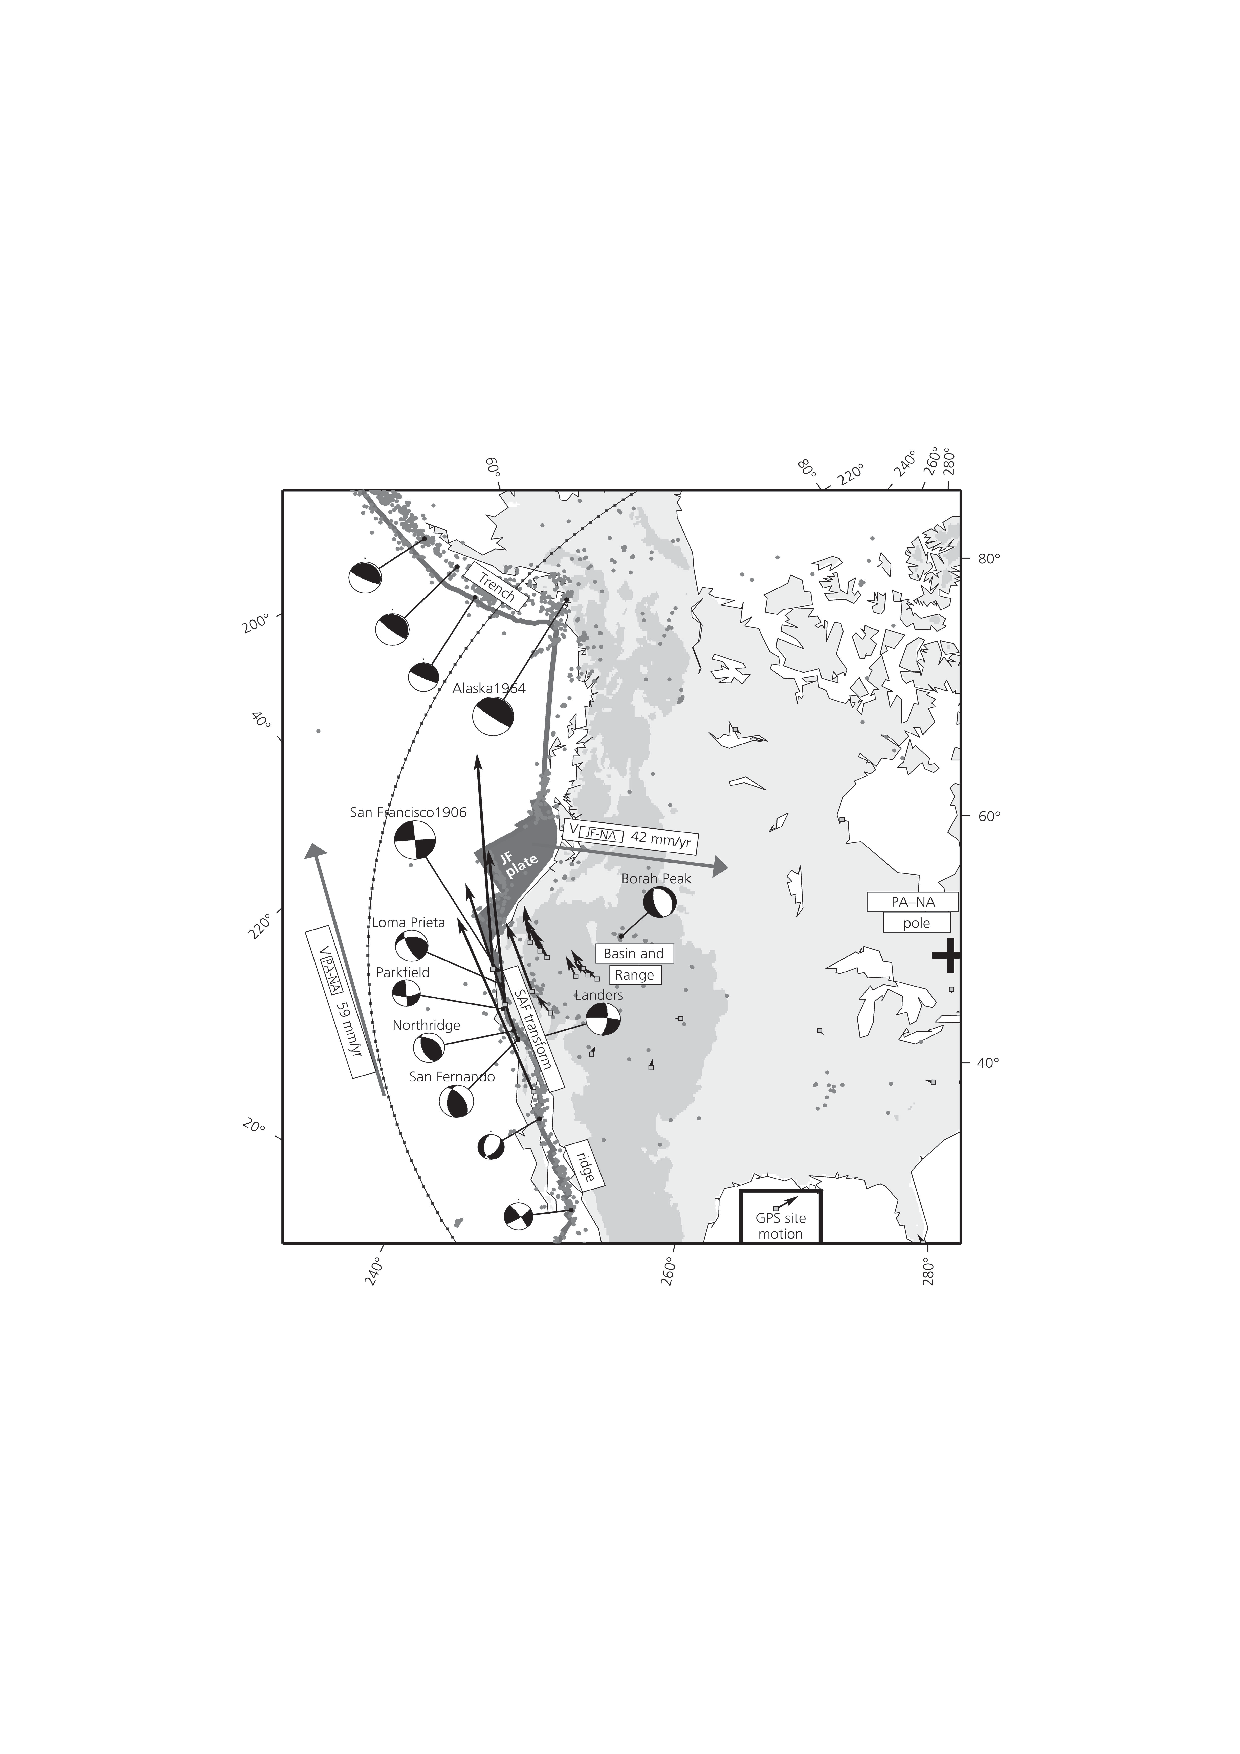
\includegraphics[trim = 0mm 70mm 0mm 70mm, clip,scale=0.6]{seismology/figures/map_with_FM.pdf}
    \caption{Map of North America with GPS movement (arrows) and earthquake
    (grey circles). Focal mechanisms indicate strike slip movements in
    California region, normal faults in Basin and Range area, and thrust
    movements in Alaska.  }
    \label{figure_map_FM}
\end{figure}

To construct a focal mechanism, only three parameters are required: the strike angle and dip angle of the fault, and the slip angle due to the earthquake displacement on the fault (see Figure~\ref{figure_fault_plan}). The strike angle $\Phi$ is defined as the angle in the plane of the earth's surface  measured clockwise from north to the fault direction ($0 \leqslant \Phi \leqslant 360$).  The dip angle $\delta$ gives the orientation of the fault plane with respect to the surface  ($0 \leqslant \delta \leqslant 90$). The final parameter is the slip angle $\lambda$ and give information about the movement : a slip angle of $\lambda$=0$^{\circ}$ indicates a \emph{left-lateral motion}; a slip angle of $\lambda$=180$^{\circ}$ shows a \emph{right-lateral motion}; a slip angle of $\lambda$=270$^{\circ}$ describes a \emph{normal faulting} ; finally a slip angle of $\lambda$=90$^{\circ}$ reveals a \emph{thrust faulting}. Sometimes, the dip angle is included between -180$^{\circ}$ to 180$^{\circ}$.
\begin{figure}[h!]
    \centering
    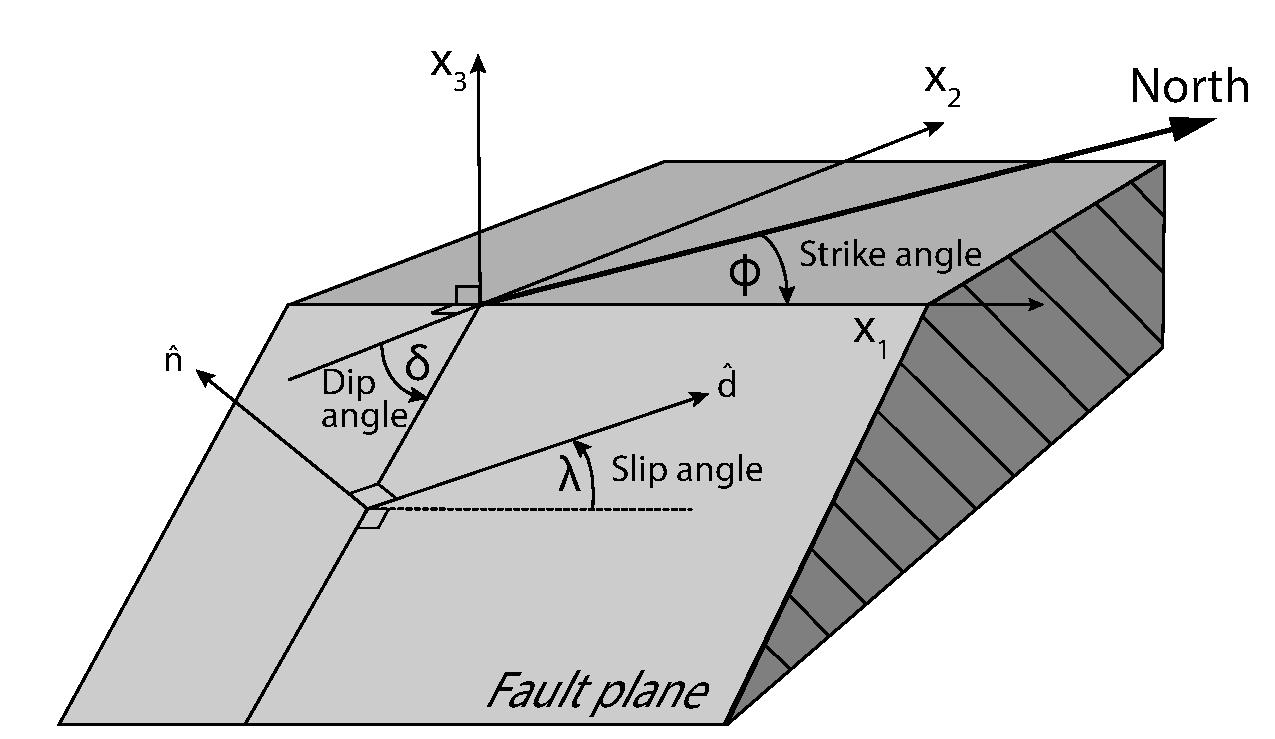
\includegraphics[trim = 0mm 140mm 0mm 0mm, clip,scale=0.5]{seismology/figures/figure_plan.pdf}
    \caption{Fault geometry used in earthquake studies.}
    \label{figure_fault_plan}
\end{figure}

Finally, we can construct the focal mechanism using stereonets and the procedure is shown for two examples in Figures~\ref{figure_FM_1} and \ref{figure_FM_2}.
\begin{figure}[h]
    \centering
    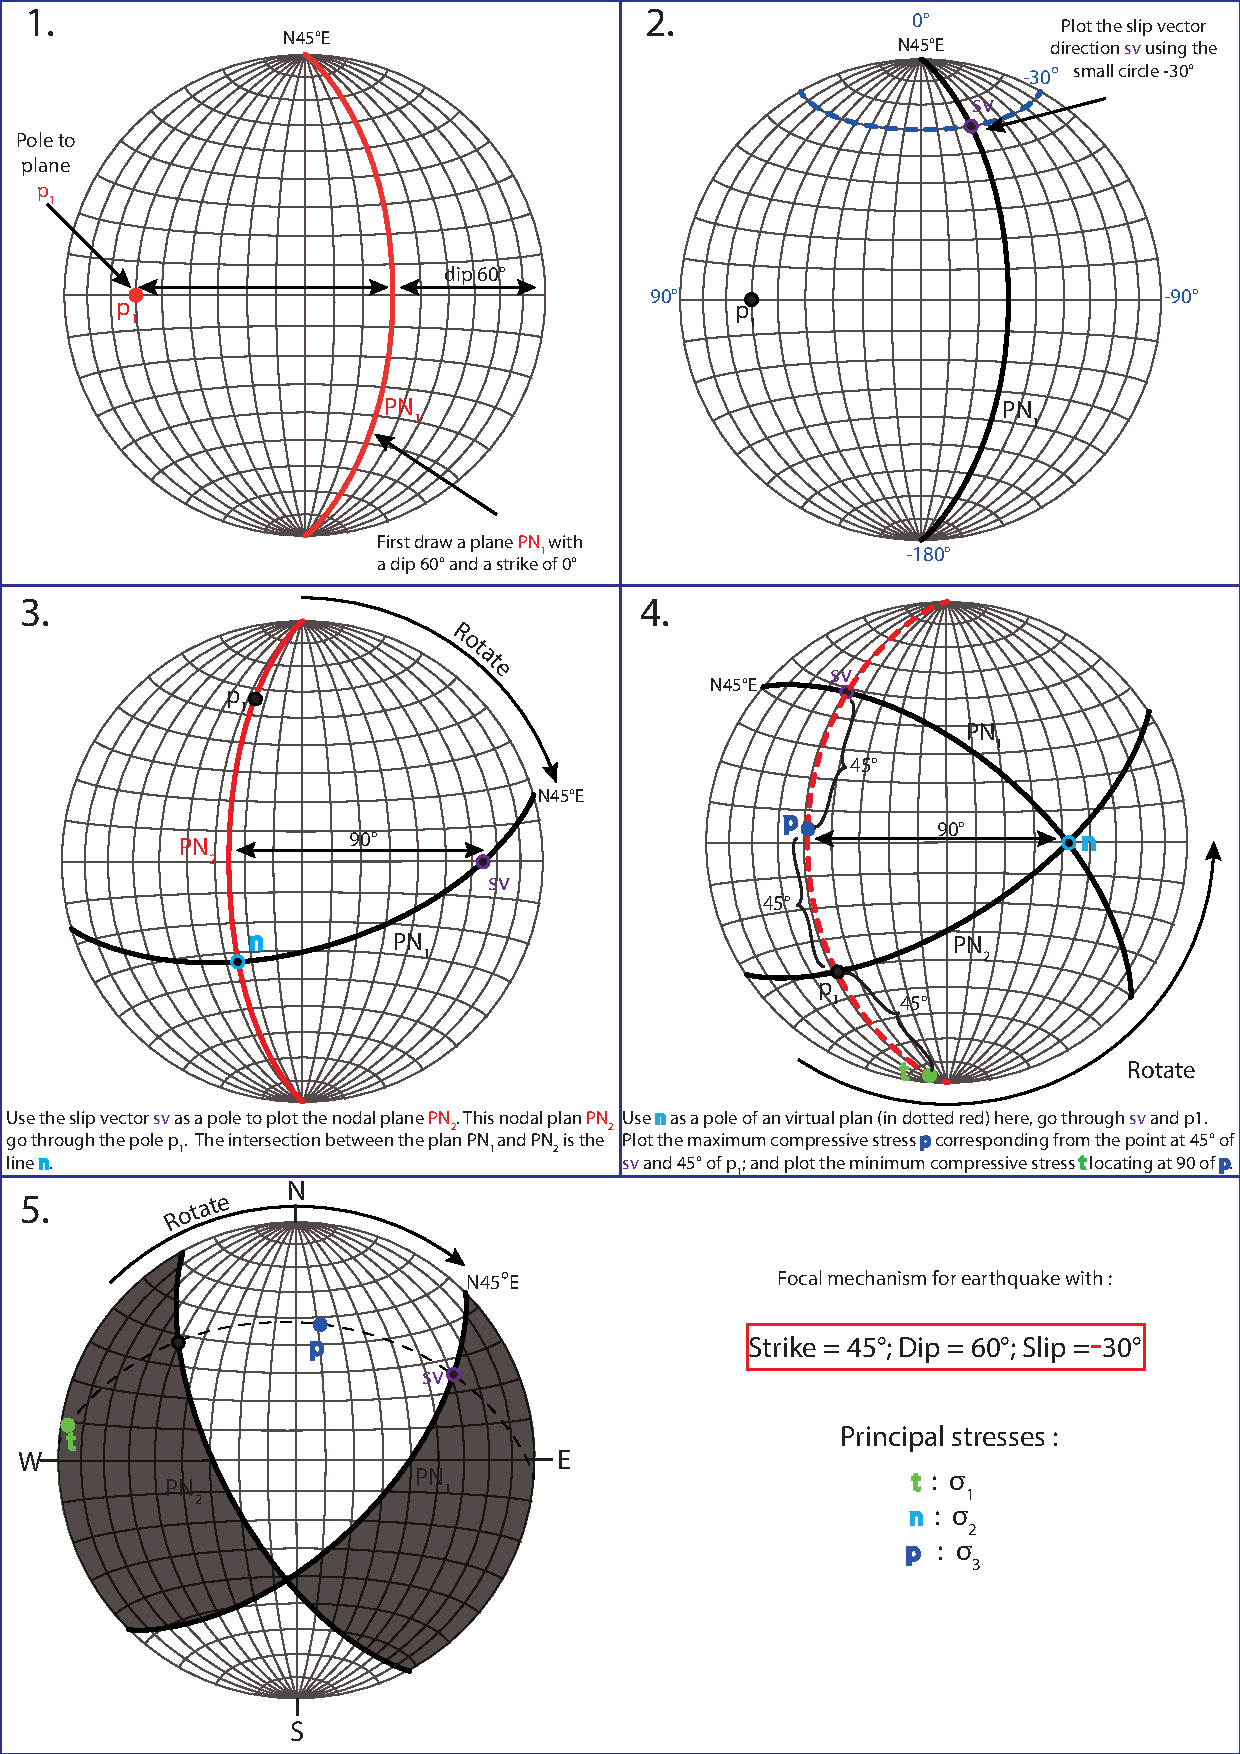
\includegraphics[trim = 0mm 0mm 0mm 0mm, clip,scale=0.6]{seismology/figures/stereonet_method_final_vertical.pdf}
    \caption{Focal mechanisms : example 1. This focal mechanism is constructed from the following parameters : $\Phi$=45$^{\circ}$; $\delta$=60$^{\circ}$; $\lambda$=-30$^{\circ}$. The 3 points $t$, $n$, and $p$ show the direction and dip of principal stresses $\sigma_1$, $\sigma_2$, and $\sigma_3$, respectively.}
    \label{figure_FM_1}
\end{figure}


\begin{figure}[h]
    \centering
    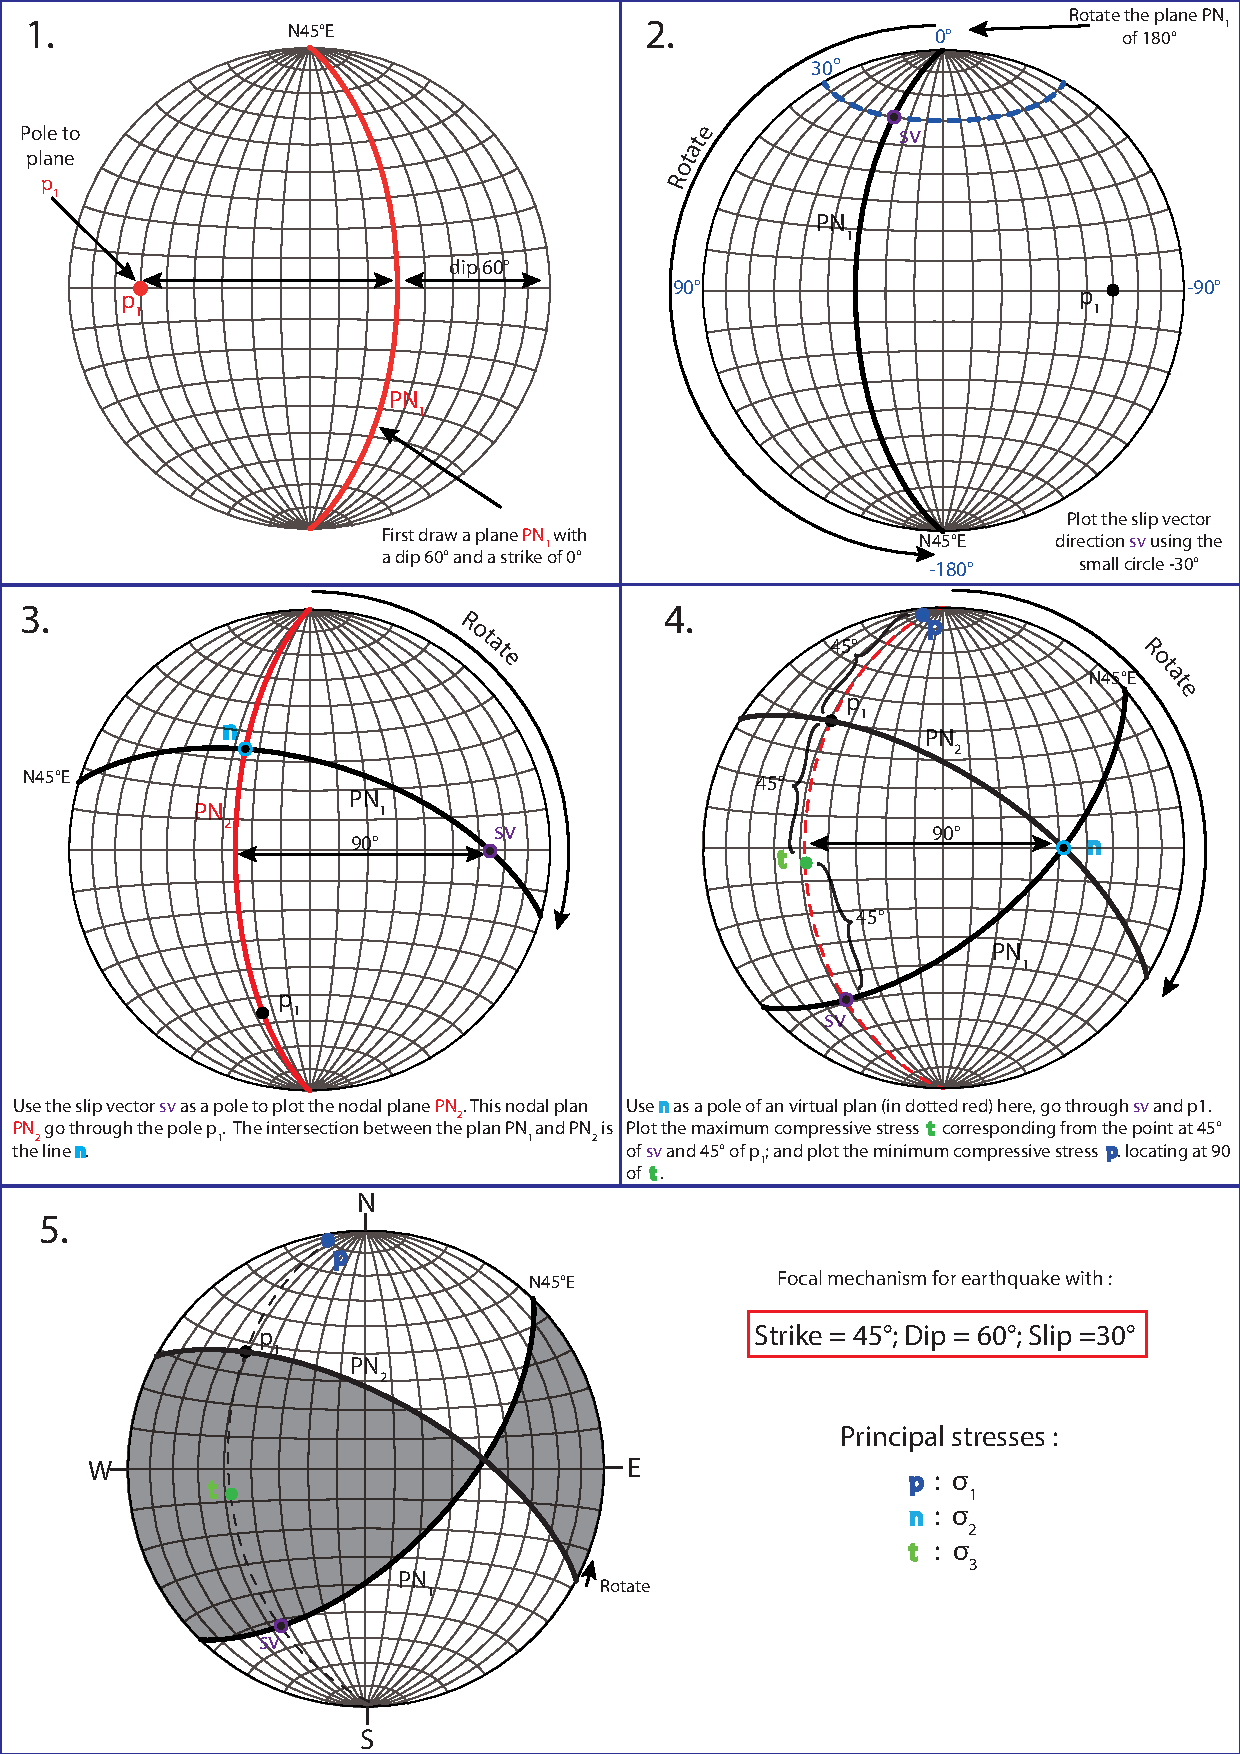
\includegraphics[trim = 0mm 0mm 0mm 0mm, clip,scale=0.6]{seismology/figures/stereonet_method_final_2_vertical.pdf}
    \caption{Focal mechanisms :  example 2. This focal mechanism is constructed from the following parameters : $\Phi$=45$^{\circ}$; $\delta$=60$^{\circ}$; $\lambda$=30$^{\circ}$.The 3 points $p$, $n$, and $t$ show the direction and dip of principal stresses $\sigma_1$, $\sigma_2$, $\sigma_3$ respectively.}
    \label{figure_FM_2}
\end{figure}


\subsection{Hudson diagram}
The Hudson diagram (a.k.a.\ source type plot, after Hudson, 1989) is useful for comparing the source types.  The center of the plot is a pure double couple (DC) solution.  Note this could be any double couple solution whether from a strike-slip, normal, reverse, or dip-slip fault.  The axis that falls between the $+$CLVD and $-$CLVD solutions represents no net volume change.  Above and below these zones, some volumetric change occurs during the rupture.
\begin{figure}[hbtp]
    \centering
    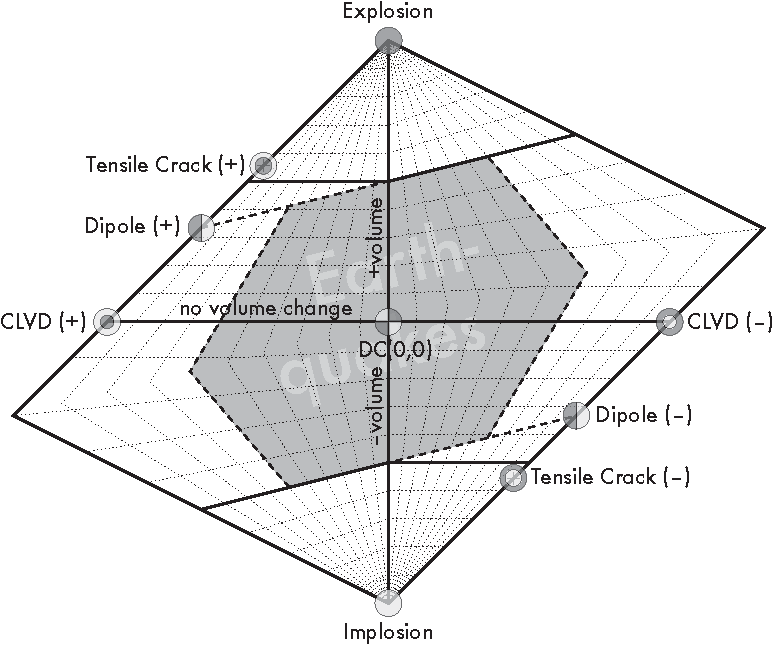
\includegraphics[]{seismology/figures/hudson_diagram2.pdf}
    \caption{Hudson diagram (source type plot) showing the distribution of possible source types.  DC is double couple (quadrupole) and CLVD is compensated linear vector dipole.  Focal mechanisms are plotted over ideal solutions to different pure source types.  Grey region is approximate region of most earthquakes.}
    \label{fig:hudson}
\end{figure}

Why might we find this useful?  For a collection of earthquakes and can help discriminate events based on multiple independent processes (Figure~\ref{fig:hudson}).  For example during volcanic eruptions, there may be several distinct episodes of magma injection and explosive volcanism.  These different source types may occur in spatially distinct regions or operate at different times.  Most earthquakes, but not all, fall within a defined region of the Hudson diagram centered about a pure double couple mechanism (grey region in Figure~\ref{fig:hudson}).

An example of a Hudson diagram for different source types is shown in Figure~\ref{fig:ford}.  Note the distinct differences in the locations of the source types.
\begin{figure}[hbtp]
    \centering
    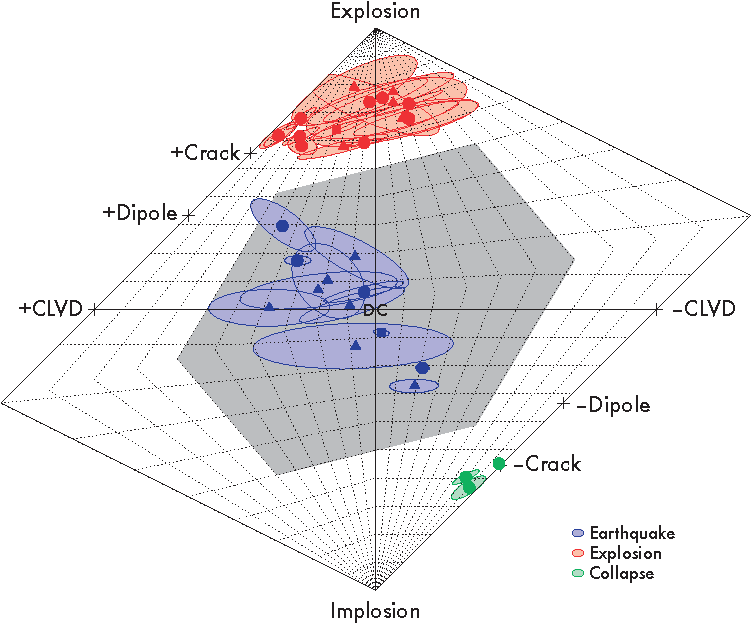
\includegraphics[]{seismology/figures/ford_etal2009_fig5.pdf}
    \caption{Source type plots for several earthquakes, nuclear explosions and
    mine collapses.  The shaded ovals represent 95\% confidence intervals.  After
    Ford et al. (2009).}
    \label{fig:ford}
\end{figure}


\section{Seismic Velocity}
The estimation of seismic velocity for minerals and rocks is discussed in Chapter~\ref{chap:physprop}.  Here we look at the effect of pressure and temperature on the seismic velocity for rocks instead of their consituent minerals.  Because models of seismic velocity estimates of the interior are more reliable than some other geophysical parameters made from surface observations, you will often find seismic velocity being used as a proxy used to estimate other physical properties.  Density is perhaps the most common of these so I include a little about the estimation of density from velocity in this section as well.

% P-T dependence
\subsection{$V_{P}$~Pressure~and~Temperature~Dependence}
Figure~\ref{fig:vpfit} illustrates the changes in seismic velocity as a function
of changes in temperature and pressure.
\begin{figure}[bthp]
    \centering
    \includegraphics[width=5.0in]{seismology/figures/gabbro.eps}
    \caption[Illustration of mathematical models used to predict seismic velocity.]{Mathematical preditions of the seismic velocity of gabbro.  P-wave velocity data of gabbro from \citet{Christensen&Mooney1995} (x's) are approximated using a pressure--temperature dependent model with (solid) and without (dashed) a crack closure term.  Each set of curves corresponds to data collected along at 20\degC\ or along a geothermal gradient of 8.9, 15.2, and 26.9\degC~km$^{-1}$.}
    \label{fig:vpfit}
\end{figure}
Each set of $V_{P}$ data corresponds to a different thermal gradient (curves labeled A (lowest) to D (highest)).  The constant temperature curve (A) shows an increase in velocity with pressure.  The other three (B--D) show a decrease in velocity with pressure because of the strong dependence of $V_{P}$ on temperature.

The effects of pressure and temperature are well known for a variety of rock types and tend to behave in a fairly predictable fashion.  Seismic P-wave velocity for a given rock can be expressed in terms of linear derivatives of pressure and temperature of the form
\begin{equation}
    V_{P}(P,T) = V^{\prime}_0
    + (T - T_{0})\left(\frac{\partial V_{P}}{\partial T}\right)_{P}
    + (P - P_{0})\left(\frac{\partial V_{P}}{\partial P}\right)_{T},
    \label{eq:pt}
\end{equation}
where $P_0$ and $T_0$ are the standard temperature and pressure conditions (STP) and $V^{\prime}_0$ is the p-wave velocity potential at STP.  The pressure and temperature deriviatives are measured in the labratory.  The pressure derivative for shallow crustal rocks is typically constant and independent of temperature at pressures up to 3 GPa \citep{Christensen&Mooney1995}.

The red curves in Figure~\ref{fig:vpfit} are computed using this model and generally fit the data well above 0.6~MPa or about 20~km depth.  So either this model is a poor approximation to the pressure affect or there are other influences on seismic velocity.  Since we know the seismic velocity of a rock is affected by several competing physical variables, including pressure, temperature, crack closure and mineral phase changes.  Since the data are most affected near the surface, it seems reasonable to assume fractures/cracks may have something to do with it.

% Crack closure
\subsection{Crack~Closure}
In the upper \SI{600}{MPa}, seismic velocities increase rapidly as a result of crack closure.  This increase is not described by Equation \ref{eq:pt}.  The effect of crack closure on seismic velocity can be generally expressed as
\begin{equation}
    V(P,T) = V^{\prime}(P,T) - f(P),
\end{equation}
where $V$ is the observed P-wave velocity and $V^{\prime}$ is the potential p-wave velocity absent the effects of cracks.  The function $f(P)$ represents the effect of crack closure on p-wave velocity.  To determine the nature of $f$, the contribution of the linear pressure derivative is removed (analagous to reduced temperature), leaving only the effects due to crack closure.  Three functional forms of $f$ were used to fit the crack effect: an inverse function, $f = a_{c}/P$; an exponential, $f = a_{c} \mbox{exp}(-P/P_{c})$; and an error function, $f = a_{c} \mbox{erfc}(P/P_{c})$.  The constant $a_{c}$ is a scaling factor and $P_{c}$ is the decay length.

An error function with a decay length $\sim$\SI{95}{MPa} best approximates the effect of crack closure on all rock samples.  At \SI{95}{MPa}, 84\% of the velocity increase due to crack closure has occurred.  Figure \ref{fig:crack}$a$ shows the a fit of the error function to a rock sample used in the analysis.  The error function describes the effect of crack closure quite well.  Unlike the decay depth, the scaling factor is much harder to determine.  Correlations between the scale factor (Figure \ref{fig:crack}$b$) and the velocity potential and density (Figure \ref{fig:crack}$c$) are very low ($r^2$ values 0.36 and 0.16).  Therefore, it appears that the scale factor is rock sample dependent and possibly the result of degree of fracturing and fracture orientations within a sample.  Once the scale factor for a particular rock has been determined, the revised function used to estimate seismic velocity becomes
\begin{equation}
    V_{P}(P,T) = V^{\prime}_{0} - a_{c} \mbox{erfc}(P/P_{c})
    + (T - T_{0})\left(\frac{\partial V_{P}}{\partial T}\right)_{P}
    + (P - P_{0})\left(\frac{\partial V_{P}}{\partial P}\right)_{T}.
    \label{eq:vp}
\end{equation}
\begin{figure}[tbhp]
    \centering
    \includegraphics{seismology/figures/crack.eps}
    \caption{Crack closure model.  $(a)$ Illustrates the best fitting crack closure model using an error function with $P_c = \SI{95}{MPa}$ (solid line).  Seismic velocity data from \citet{Kern_etal1999} are plotted as x's.  $(b)$ and $(c)$ displays the scaling factor as a function of potential seismic velocity and density.}
    \label{fig:crack}
\end{figure}
The velocity potential is determined by extrapolating the high pressure velocites unaffected by cracks to the surface.  A major difference between the data used to determine the $V_{P}$ relationship and model the the crack closure depth is the crack closure depth.

The fit of Equations~\ref{eq:pt} (dashed) and \ref{eq:vp} (solid) to the velocity data in Figure~\ref{fig:vpfit} shows the importance of a crack closure term below 600~MPa.  The fit of modeled crack effect on $V_{P}$ to the labratory data of gabbro shows a significant improvement over the purely $P$--$T$ model.

% Estimating Density
\subsection{Estimating~Densities}
The density increase with pressure can be described using a simple linear
relationship,
\begin{equation}
    \rho{_P} = \rho_{0} + (P - P_0)\left(\pdv{\rho}{P}\right)_T,
\end{equation}
where $\rho_{0}$ is surface density and $\left(\partial \rho/\partial P\right)$ is the pressure derivative of density at constant temperature.  The pressure derivative must be determined for each rock type based on experimental data.  A linear fit to the density data in \citet{Christensen&Mooney1995} yields a factor of 3 range of pressure derivatives from 15.6 to \SI{42}{kg.m^{-3}.MPa^{-1}} with a median of \SI{29.7}{kg.m^{-3}.MPa^{-1}}.  Temperature effects on density are not accounted for in the analysis by \citet{Christensen&Mooney1995} and are potentially larger than the effects of pressure.

An example of the fit to density is shown in Figure~\ref{fig:vprho}
\begin{figure}[tbhp]
    \centering
    \includegraphics{seismology/figures/velocity_to_density.eps}
    \caption{Velocity to density models fit to a number of rocks types.  Two models are shown for igneous and metamrophic rocks (red) by {\citet{Christensen&Mooney1995}}. The \citet{Barton1986} model was developed for sedimentary rocks (grey).  The yellow points are monomineralic rocks not included in fit.}
    \label{fig:vprho}
\end{figure}

The prefered model used to estimate the density from seismic velocity is given by the linear seismic velocity to density relationship \citep{Christensen&Mooney1995} given by
\begin{equation}
  \label{eq:cmlinear}
  \rho = a + b V_{P},
\end{equation}
where $a$ and $b$ are empirically derived coefficients.  \textit{Christensen and Mooney} published coefficients to the linear $V_{P}$--$\rho$ equation for a temperature of \si{309}{\degC}\ and pressures equivalent to 5 to 50~km in increments of 5~km.  Therefore, it is necessary to determine the coefficients to all other crustal $P$--$T$ conditions for this study.  Having developed a method to extend density and seismic velocity to a greater range of $P$--$T$ conditions, the empirical coefficients are determined using a linear least-squares inversion to polymineralic rock types at the range of crustal pressures ranging from 0 to 2.6~GPa and temperatures from 20 to \si{1300}{\degC}.  Monominearlic rock types are excluded from determining the coefficients in the linear relationship as they tend to have high velocities with low density or vice versa. Figure~\ref{fig:empconst}
$a$ and $b$ contour the linear coefficients ($a$ and $b$ from Equation~\ref{eq:cmlinear}) for an extended range of pressure and temperature conditions
for the depth and temperature.
\begin{figure}[tbhp]
    \centering
    \includegraphics{seismology/figures/CM95linear.eps}
    \caption[Empirical coefficients for the linear $V_{P}$--$\rho$ conversion by \citet{Christensen&Mooney1995}.]{Empirical coefficients for the linear $V_{P}$--$\rho$ conversion by \citet{Christensen&Mooney1995} are gridded for range of possible $P$--$T$ conditions.}
    \label{fig:empconst}
\end{figure}
%\FloatBarrier

\ntextbox{Stress Fields Across Regimes: Static, Diffusive, and Wave Behavior}{
    With so many geophysical fields bridging the various PDE realms, you may be asking yourself whether elastic fields---seismic fields are elastic waves---admit similar steady-state and diffusive behaviors.  The short answer is no, not directly; but the longer answer is that elastic stress fields do exhibit elliptic, parabolic and hyperbolic regimes, but these operate on different spatial and temporal scales and are not observed in the same way as classical geophysical fields, as summarized below.

    Stress and strain in the solid Earth are governed by the same underlying mechanical framework, but admit distinct mathematical regimes depending on the relative importance of inertia and dissipation. These regimes operate on different spatial and temporal scales and are sampled by different observational approaches.

    \begin{enumerate}
        \item \textbf{Static (Elastic Equilibrium)}

        In the absence of inertia, long-term tectonic stresses satisfy the equations of static elasticity:
        \[
            \div{\bm{\sigma}} + \vb{f} = 0, \quad \bm{\sigma} = \vb{C} \colon \bm{\varepsilon}, \quad \bm{\varepsilon} = \tfrac{1}{2}(\grad{\vb{u}} + \grad{\vb{u}^\mathsf{T}}),
        \]
        where $\vb{f}$ is the body force per unit volume, and $\vb{C}$ is the fourth-order elastic stiffness tensor.

        This system is elliptic and defines a boundary-value problem for displacement and stress. Static stress fields reflect present-day plate boundary forces and loads, modified by elastic structure and heterogeneity. Although well-posed mathematically, stress is not directly observable at depth; surface measurements are sparse, load-contaminated, and path-dependent.

        \item \textbf{Diffusive (Stress Relaxation)}

        When dissipation is introduced through viscoelastic or poroelastic behavior, stress evolves diffusively at long times:
        \[
            \pdv{\bm{\sigma}}{t} = D_\sigma \,\laplacian{\bm{\sigma}}, \quad D_\sigma \sim \frac{\mu}{\eta},
        \]
        where $D_{\sigma}$ is the effective stress diffusivity.

        This parabolic regime governs postseismic deformation and long-term tectonic relaxation, primarily within the ductile lower crust and upper mantle. The characteristic timescale is the Maxwell relaxation time, $\tau_M = \eta/\mu$, where $\eta$ is the effective viscosity and $\mu$ is the shear modulus.

        which typically ranges from decades to thousands of years depending on rheology. In the continental crust, effective relaxation times are commonly $10^1--10^3$ years, while in the upper mantle they may be shorter where viscosities are lower. This diffusive regime underlies postseismic deformation, where stress perturbations introduced by earthquakes relax through viscoelastic flow and poroelastic pressure diffusion. Observational access to this regime is indirect, relying on geodetic measurements (e.g., GPS, InSAR) rather than traditional geophysical field observations.

        \item \textbf{Wave Propagation (Seismology)}

        Including inertia yields the elastic wave equation:
        \[
            \rho \, \pdv[2]{\vb{u}}{t} = \div{(\vb{C} \colon \grad \vb{u})},
        \]
        which is hyperbolic and supports propagating seismic waves. This regime samples transient stress disturbances rather than the background stress field. Wave propagation does not relax to a steady-state or diffusive limit; once energy propagates away, the field vanishes.
    \end{enumerate}

    \noindent\textbf{Interpretation and Observability}\\
    Although static and diffusive stress fields are physically real and mathematically well defined, they do not constitute classical geophysical field methods because stress is not directly observable at depth. Consequently, these regimes are treated primarily within geodesy and tectonics, while seismology focuses on the hyperbolic, wave-propagation regime where signals are directly measurable.  This distinction mirrors that between elliptic, parabolic, and hyperbolic governing equations encountered elsewhere in geophysics, but highlights that the existence of a governing PDE does not guarantee a usable geophysical observable.
}{aside}


\nocite{Fowler1990}
\nocite{Lowrie1997}
\nocite{Schey1997}

\bibliographystyle{elsarticle-harv}
\bibliography{ref}

\chapter{Seismics}\label{ch:seismics}
\section{Introduction}
\subsection{Key concepts}
\begin{itemize}

    \item What is a wavefront? a ray-path?  What is travel-time and how does it
    relate to a ray-path?

    \item Know Snell's law.  What is the critical angle?

    \item What is reflection?  Be able to set up a reflection problem
    (travel-times related to lengths of ray-path segments).  When does a
    reflection occur (related to acoustic impedance)?  What is the shape of the
    travel-time function for a reflection?

    \item What is refraction?  Be able to set up a refraction problem
    (travel-times related to lengths of ray-path segments).  When does a
    refraction occur (related to velocities)?  What is the shape of the
    travel-time function for a refraction?

    \item What is the relationship between reflections and refractions?
\end{itemize}

\subsection{Mathematical symbols and units}

\begin{table}[hbtp]
    \centering
    \caption{Definitions of symbols.}
    \label{tab:seismosym}
    \begin{tabular}{@{}cll@{}}
        \toprule
        \textbf{Symbol} &
        \textbf{Quantity} &
        \textbf{SI Unit} \\
        \midrule
        $t$             & time                          & second, \si{s} \\
        $x$, $y$, $z$   & distance                      & meter, \si{m} \\
        $\theta$        & angule                        & \si{rad} or \si{^\circ} \\
        \bottomrule
    \end{tabular}
\end{table}

The term {\bf seismics} typically implies active source seismology techniques that are used to investigate crustal architecture.  Much of the mathematics used to describe the behavior of seismic waves employ the theories originally developed for explaining phenomena associated with propagation of light rays.

\subsection{Wavefronts and rays}

Consider some point at the surface where an impulse is generated (S).  Waves spherically spread from the source due to the impulse much as ripples from a pebble dropped in a pond.  Alternatively, we can imagine rays that radially emanate from the source.  An important approach for wave propagation was explained by Huygens: each point on a wave front is considered to be a new source that gives rise to another circular wavefront.  These wavefronts interfere constructively to give a circular wave front, and interfere destructively everywhere else. In seismic, this principle produces the refracted and reflected waves (Figure~\ref{figure_huygens_refracted_reflection}).
\begin{figure}[hbpt]
    \centering
    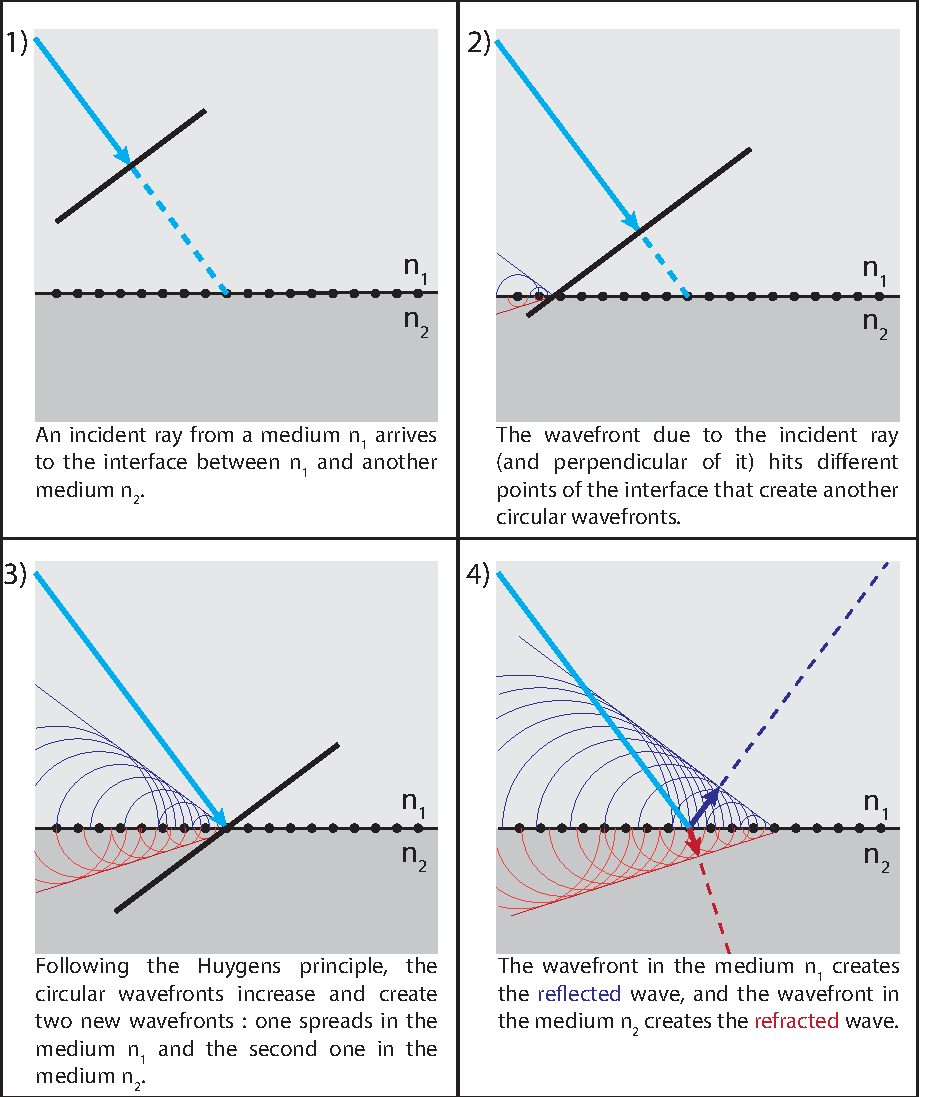
\includegraphics[trim = 0mm 100mm 30mm 0mm, clip,scale=0.7]{seismology/figures/huygens_explanation.pdf}
    \caption{Illustration of Huygens' principle. This phenomenon explains the creation of the reflected and refracted waves.}
    \label{figure_huygens_refracted_reflection}
\end{figure}
In optics, this principle allows to explain another complex phenomenon as the
diffraction .  At all times, the ray paths are normal to the wavefront
(Figure~\ref{fig:wr}).  As the wavefronts interact with boundaries between
differing velocity and/or acoustic impedance the wavefronts can reflect,
refract, and diffract.
\begin{figure}[hbtp]
    \centering
    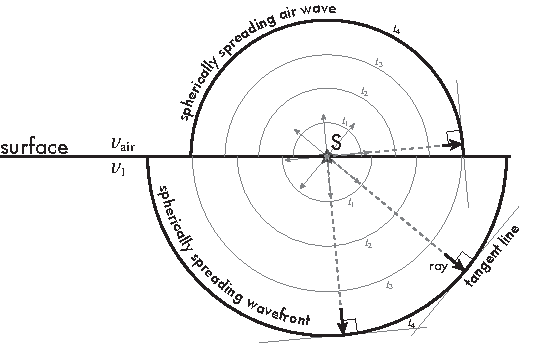
\includegraphics[]{seismology/figures/wavefronts&rays.pdf}
    \caption{Spherically spreading waves.  Rays paths are at right angles to the wavefront at all times.  What must be the relationship between the velocity of the wave in air versus the ground in this example?  Why?}
    \label{fig:wr}
\end{figure}

We will define the travel-time, $t$, as the minimum time that it takes a ray to
travel from a source, S, to any point, R, by
\begin{equation}
    t = \min \int_{\mathrm{S}}^{\mathrm{R}} \frac{\dd{\ell}}{v(x,y,z)},
\end{equation}
where $v$ is the velocity of the medium and $\dd{\ell}$ is the infinitesimal
length along the ray path.  The travel-time relationship is called Fermat's
principle.  In general the points that we care about are the receiver locations,
$\mathrm{R}_{n}$.

\subsection{Direct waves}
At some distance from the source, we place a receiver (R).  There are two waves
that directly travel from the source to the receiver, an {\bf air wave} which
travels just above the ground surface and a {\bf direct wave} which travels just
below the surface (Figure~\ref{fig:exwaves}).  There are also surface waves
(Love and Raleigh) which travel directly from the source to the receiver
(a.k.a.\ {\bf ground roll}), but they are not properly described by the ray
theory.  In general surface waves are a noise source for the types of
experiments that we are discussing.
\begin{figure}[hbtp]
    \centering
    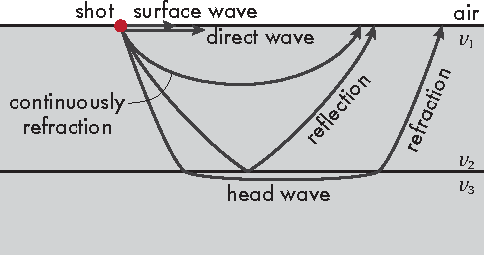
\includegraphics[]{seismology/figures/exploration_waves.pdf}
    \caption{Terminology of wave types emanating from an active source.}
    \label{fig:exwaves}
\end{figure}

For a direct wave, the travel-time between the source, S, and receiver, R,
separated by a distance, $d$, is
\begin{equation}
    t = \frac{\ell_{\mathrm{SR}}}{v_1} = \frac{d}{v_{1}},
\end{equation}
where $v_1$ is the constant velocity of the surface layer.


\subsection{Acoustic Impedance}
There are several types of indirect waves that are possible.  A ray travels
until it reaches an interface.  At the interface, some of the energy is
reflected and the remainder is transmitted.  The amount of energy that is
transmitted or reflected at a boundary is dependent upon the relative acoustic
impedance of the two layers.  We define the acoustic impedance of layer $j$ as,
$Z_j = \rho_j V_j$, where $\rho_j$ is the layer density and $V_j$ is the layer
velocity.  We can estimate the reflection coefficient, $R$, and transmission
coefficient, $T$, of a normally incident wave as
\begin{equation}
    R = \frac{Z_2 - Z_1}{Z_2 + Z_1} \mbox{ and }
    T = \frac{2 Z_1}{Z_2 + Z_1},
\end{equation}
respectively, where $R + T = 1$.  Note the similarity between these coefficients
and the complementary results from electromagnetic waves.  Since the reflection
coefficient depends upon the density as well as the velocity, a change in
velocity does not necessarily imply a reflection is guaranteed to occur.  Why
might the velocity decrease, but density increase? Or conversely, why density
decrease but velocity increase?


\subsection{Reflection}
Let us consider the constant velocity case where the ray strikes a horizontal
interface at an incident angle $\theta_i$ w.r.t.\ the vertical.  The wave is
reflected toward the surface at a reflection angle $\theta_i'$ w.r.t.\ the
vertical.  The ray travels from the source (S), bounces off an layer interface
at a point (B) a disstance $x$ from S, and is reflected to the surface and
measured at a receiver (R) a distance $d$ from S (Figure~\ref{fig:reflect}).
\begin{figure}[hbtp]
  \centerline{
    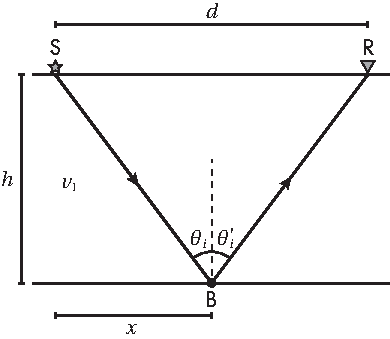
\includegraphics[]{seismology/figures/reflection.pdf}
  }
  \caption{Reflection of seismic waves.}
  \label{fig:reflect}
\end{figure}

We wish to find the minimum travel-time necessary for this path, which can be simply written as the sum of the travel-times from the source to the bounce point (SB) and the bounce point to the receiver (BR),
\begin{equation}
    t = \frac{\ell_{\mathrm{SB}}}{v_1} + \frac{\ell_{\mathrm{BR}}}{v_1} =
        v_1^{-1} \left[ (h^2 + x^2)^{1/2} + (h^2 + (d - x)^2)^{1/2} \right].
\end{equation}
To find the minimum, we take the derivative w.r.t.\ $x$ and set equal to zero,
\begin{equation}
    \dv{t}{x} = 0 = v_1^{-1}
        \left[ \frac{x}{(h^2 + x^2)^{1/2}} 
        - \frac{d - x}{(h^2 + (d - x)^2)^{1/2}} \right].
\end{equation}
Solving for $d$, we find
\begin{equation}
    d = 2 x,
\end{equation}
which implies that $\theta_i = \theta_i'$.

Hence we can write the travel-time for a reflected wave as
\begin{align}
    t(x) & = \frac{2}{v_1}
        \left[ h^2 + \left( \frac{x}{2} \right)^2 \right]^{1/2},\\
        & = \frac{2 h}{v_1}
        \left[ 1 + \left( \frac{x}{2 h} \right)^2 \right]^{1/2},
\end{align}
where $x$ is now the distance between the source and receiver.  The shape of this reflection travel-time function is a hyperbola with asymptotes at $t = \pm x v_1^{-1}$.

When the source and receiver are co-located ($x = 0$), the travel-time for a reflection is
\begin{equation}
    t_0 = \frac{2 h}{v_1}.
\end{equation}
This result allows us to write $t(x)$ in terms of $t_0$,
\begin{align}
    t(x) &= t_0 \left[ 1 + \left( \frac{x}{2 h} \right)^2 \right]^{1/2} \\
    &= t_0 \left[ 1 + \left( \frac{x}{t_0 v_1} \right)^2 \right]^{1/2},
\end{align}

\subsubsection{Normal Moveout}
Typically when we collect geophysical data, the data we collect can be modeled by physical principles.  However, we often do not know all or most of the physical parameters that result in the response that we observe.  For example, in the case above, we have derived a physical expression for the travel-time.  But our result is dependent upon the unknown parameters for the thickness of the layer and its velocity.  For the case of reflections, a method called {\bf normal moveout} is employed and whos description is given below.

Let us define a parameter called the normal moveout $t_{\mathrm{NMO}}(x) = t(x) - t_0$,
\begin{equation}
    t_{\mathrm{NMO}} = t_0 \left[ 1 + \left( \frac{x}{2 h} \right)^2 \right]^{1/2} - t_0.
\end{equation}
If we collect our data such that our geophones are close to the source w.r.t.  the depth of the layer ($x \ll h$), we can use a Taylor series expansion to write
\begin{equation*}
    t_{\mathrm{NMO}} = t_0 \left[ 1 + \frac{1}{2}\left( \frac{x}{2 h} \right)^2
    + \cdots \right] - t_0,
\end{equation*}
Ignoring terms higher than $x^2$, we find
\begin{align}
    t_{\mathrm{NMO}} & = \frac{1}{2}\left( \frac{x}{2 h} \right)^2, \\
        & = \frac{x^2}{2 v_1^2 t_0}. \\
\end{align}

We have now derived an expression for the normal moveout with respect to only one unknown, the velocity.  Once we solve for the velocity, we can then solve for the layer thickness using the expression for $t_0$.


\subsection{Refraction}
Refraction refers to the bending of a wave at a boundary due to a contrast in physical properties.  In our case, the physical property that results in bending the waves is the velocity of the medium.

Let us consider, as before, the constant velocity case where the ray strikes a horizontal interface at an incident angle $\theta_i$ w.r.t.\ the vertical (Figure~\ref{fig:refract}).  The wave is transmitted through the lower medium, but is refracted by an angle $\theta_r$ w.r.t.\ the vertical.  The ray travels from the source (S), bends at the layer interface at a point (B), and is measured at a point (R) a horizontal distance $d$ from the source.
\begin{figure}[hbtp]
  \centerline{
    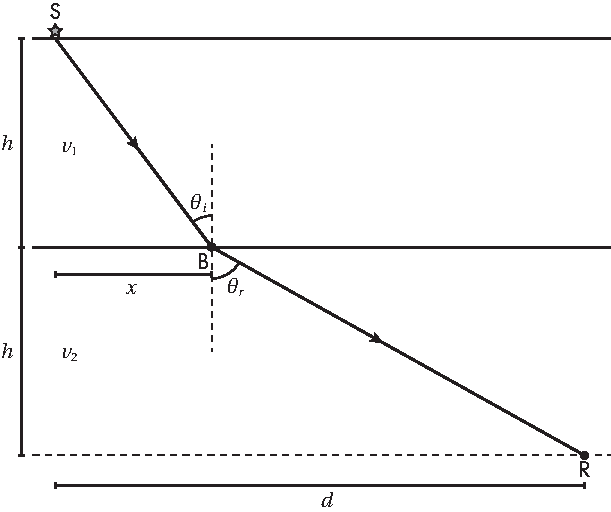
\includegraphics[]{seismology/figures/refraction.pdf}
  }
  \caption{Refraction of seismic waves.}
  \label{fig:refract}
\end{figure}

The travel-time from S to R may be written as the sum of the travel-times from
SB and BR,
\begin{equation}
    t = \frac{\ell_{\mathrm{SB}}}{v_1} + \frac{\ell_{\mathrm{BR}}}{v_2} =
        \frac{(h^2 + x^2)^{1/2}}{v_1} + \frac{(h^2 + (d - x)^2)^{1/2}}{v_2} .
\end{equation}
To find the minimum, we take the derivative w.r.t.\ $x$ and set equal to zero,
\begin{equation}
    \dv{t}{x} = 0 = 
        v_1^{-1}\frac{x}{(h^2 + x^2)^{1/2}} 
        - v_2^{-1}\frac{d - x}{(h^2 + (d - x)^2)^{1/2}} .
\end{equation}
We can use the trigonometric relations to rewrite the above result as
\begin{equation}
    \frac{\sin \theta_i}{v_1} = \frac{\sin \theta_r}{v_2}.
\end{equation}
This relation is known as Snell's Law.  Unlike reflection where reflections only occur at interfaces with differing impedance, not simply differing velocity, refractions occur when the velocities differ at an interface.

If the velocities are such that $v_2 > v_1$, then the ray is bent toward the interface, $\theta_r > \theta_i$.  There exists a critical incidence angle, $\theta_c$, such that the wave is refracted parallel to the layer interface, i.e.\ critically refracted (Figure~\ref{fig:cr}).  The critical angle occurs when $\theta_r = \frac{\pi}{2} = 90^\circ$.  This allows us to solve for the critical angle in terms of the velocity ratio
\begin{equation}
    \sin \theta_c = \frac{v_{1}}{v_2}.
\end{equation}
\begin{figure}[hbtp]
    \centering
    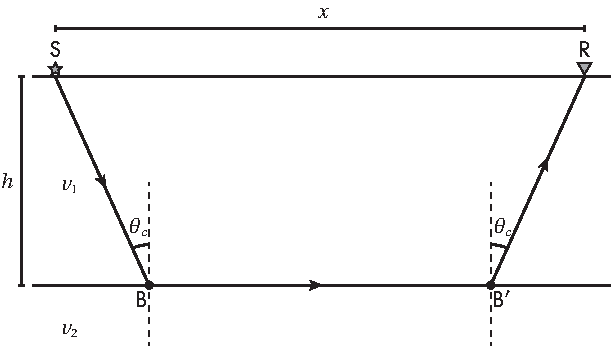
\includegraphics[]{seismology/figures/critical_refraction.pdf}
    \caption{Critical angle and double refraction of seismic waves.}
    \label{fig:cr}
\end{figure}

Critically refracted waves are important as they continuously refract back up into the layer above and return to the surface.  The travel-time for a refracted wave between the source, S, and a receiver, R, can be found by tracing a ray from the source at an angle critical to the interface, along the interface, and from the interface to the receiver at the critical angle,
\begin{equation}
    t = \frac{\ell_\mathrm{SB}}{v_1} + \frac{\ell_\mathrm{BB'}}{v_2} +
    \frac{\ell_\mathrm{B'R}}{v_1}.
\end{equation}
For a horizontal layer, the lengths SB and B'R are equal.  The resulting
travel-time is
\begin{equation}
    t = 2 \frac{h}{v_1 \cos \theta_c} + \frac{x - 2 h \tan \theta_c}{v_2}.
\end{equation}
We can simplify the above result somewhat by rearranging terms
\begin{align*}
    t & = \frac{x}{v_2} + 2 h
        \left( \frac{1}{v_1 \cos \theta_c}
        - \frac{\sin \theta_c}{v_2 \cos \theta_c} \right), \\
    & = \frac{x}{v_2} + 2 h
        \left( \frac{v_2 - v_1 \sin \theta_c}{v_1 v_2 \cos \theta_c} 
         \right),
\end{align*}
at this point we can use Snell's Law ($\sin \theta_c = \frac{v_1}{v_2}$),
\begin{align*}
    t & = \frac{x}{v_2} + 2 h
        \left( \frac{v_2 - v_2 \sin^2 \theta_c}{v_1 v_2 \cos \theta_c} \right), \\
    & = \frac{x}{v_2} + 2 h
        \left( \frac{1 - \sin^2 \theta_c}{v_1 \cos \theta_c} \right),
\end{align*}
recalling $\cos^2 \theta + \sin^2 \theta \equiv 1$, we arrive at
\begin{equation}
    t = \frac{x}{v_2} +
        \frac{2 h \cos \theta_c}{v_1} .
\end{equation}
If we wish, we may remove the dependence upon $\theta_c$ and write the result in terms of the velocities as
\begin{align}
    t & = \frac{x}{v_2} +
        \frac{2 h (v_2^2 - v_1^2)^{1/2}}{v_1 v_2} , \\
      & = \frac{x}{v_2} +
      2 h \left( \frac{1}{v_1^2} - \frac{1}{v_2^2} \right)^{1/2}.
\end{align}

The resulting travel-time for a doubly refracted wave is the equation of a line (i.e.\ $t = m x + t_i$) with the slope $m = \frac{1}{v_1}$, and intercept time
\begin{align}
    t_i = \frac{2 h (v_2^2 - v_1^2)^{1/2}}{v_1 v_2} .
\end{align}

While reflections occur whenever there is an acoustic impedance, a refracted wave only occurs when $\theta = \theta_c$.  Hence, at receiver locations within a given proximity of source, a refracted wave cannot physically appear.  If $v_1 > v_2$ then the ray is bent away from the interface, $\theta_i > \theta_r$.  As a result, the waves cannot be critically refracted and will not return to the surface.  While refractions can still occur from deeper layers, the effect of a low velocity layer beneath a higher velocity is hidden and results in a larger predicted thickness of the layer below the low velocity zone.

%\subsection{Tomography}
%So far, we have only described seismic waves traveling through layered media, 

\nocite{Grant&West1965}

\bibliographystyle{elsarticle-harv}
\bibliography{ref}


\part{Computational and Inverse Methods}
% Numerical methods
\chapter{Fourier Series}\label{ch:fourier_series}
\section{Introduction}

Fourier series arise naturally in geoscience when we seek analytical solutions to physical problems defined on finite domains and subject to boundary conditions. Many governing equations in geophysics—most notably Laplace's equation and the diffusion (heat) equation—can be solved using separation of variables, leading to solutions expressed as sums of orthogonal sine and cosine functions. In this context, the functions themselves are unknown, and the role of the Fourier series is to construct a field that simultaneously satisfies the governing differential equation and the imposed boundary conditions.

Fourier series are therefore especially important in problems involving thermal conduction, electrostatics, and gravitation, where the objective is to determine temperature, potential, or field distributions within a bounded region of space. Examples include steady-state and time-dependent heat flow in the lithosphere, electric potential distributions in the Earth, and idealized gravity or magnetic potentials near interfaces. In these applications, the discrete eigenfunctions arising from the boundary conditions have direct physical meaning, and the Fourier coefficients describe how strongly each mode contributes to the total solution.

Although Fourier series are less commonly applied directly to geophysical data analysis, they provide essential conceptual foundations for understanding how boundary conditions, scale, and orthogonality shape physical solutions. As such, Fourier series should be viewed not as a signal-processing tool, but as an eigenfunction method for solving partial differential equations that describe geophysical processes.

Fourier series and transforms are used to
\begin{itemize}
    \item identify dominant wave frequencies within a signal, perhaps due to some physical process;
    \item filter data to emphasize aspects of a signal and/or eliminate outliers;
    \item reduce the quantity of information needed to store a signal and transmit a signal (basically how your mobile phone works);
    \item solve certain partial differential equations;
    \item and \ldots .
\end{itemize}


\section{Periodic Functions and Modes}

Many physical problems in geoscience involve quantities that vary in a repeating or quasi-repeating way, either in time or in space. Such behavior is referred to as \textbf{periodic} and is central to the development of Fourier series. Before introducing the formal mathematics, it is helpful to understand what periodicity means physically and why it leads naturally to discrete modes in bounded domains.

\subsection{Periodicity in Space and Time}

A function is said to be periodic if it repeats after a fixed interval. In the temporal case, a function $f(t)$ is periodic with period $\tau$ if
\[
    f(t + \tau) = f(t),
\]
while in the spatial case a function $f(x)$ is periodic with wavelength $\lambda$ if
\[
    f(x + \lambda) = f(x).
\]

Periodic behavior arises in many geophysical contexts. Temporal periodicity is associated with repeating processes such as seismic wave motion, tidal forcing, and climatic cycles. Spatial periodicity appears in layered media, interference patterns, and idealized models of geological structure. Even when natural systems are not perfectly periodic, treating them as such over a limited domain often leads to useful approximate solutions.

\subsection{Sine and Cosine as Repeating Building Blocks}

Among all periodic functions, sine and cosine play a special role. They are smooth, continuous, and naturally repeating, and many physical systems governed by linear differential equations admit solutions that can be expressed as combinations of these functions. Because of this, sine and cosine functions are convenient building blocks for constructing more complicated shapes.

Importantly, sine and cosine functions repeat exactly and do so without introducing sharp corners or discontinuities. This makes them well suited for representing physical fields such as temperature, potential, or displacement, which are typically smooth in space and time. By combining sine and cosine functions of different spatial scales, it is possible to approximate a wide range of physically reasonable functions.

Sine and cosine functions are smooth and infinitely differentiable, which makes them well suited for representing smooth physical fields. However, when a function contains sharp discontinuities or non-differentiable interfaces, many modes are required to represent those features accurately, and oscillatory behavior may appear near the discontinuities.

\subsection{Wavelength and Scale in Geological Terms}

In spatial problems, the scale of variation is commonly described by the \textbf{wavelength}, which is the distance over which a function completes one full cycle. Long wavelengths correspond to slowly varying features, while short wavelengths represent rapid spatial changes.

In geophysics, wavelength often has a direct physical interpretation. For example, long-wavelength variations in gravity or magnetic fields are typically associated with deeper sources, whereas short-wavelength variations tend to reflect shallow structure. Similarly, in thermal problems, long spatial scales may correspond to broad regional trends, while short scales reflect near-surface effects.

Thinking in terms of wavelength therefore provides an intuitive way to connect mathematical representations to geological structure.

\subsection{Allowed Wavelengths in a Bounded Domain}

A crucial distinction between Fourier series and other Fourier methods is that Fourier series are used for functions defined on \emph{finite} domains. When a domain has finite extent, the possible spatial patterns that can exist within it are constrained.

Consider a function defined on the interval $0 \le x \le L$. For the function to behave consistently within this domain, it must satisfy specific conditions at the boundaries. These requirements restrict which wavelengths can fit into the interval in a self-consistent way. Only wavelengths that allow an integer number of half-cycles or full cycles within the domain are permitted.

As a result, the function can be represented only by a \emph{discrete set} of spatial patterns, often referred to as modes. Each mode corresponds to a particular allowed wavelength determined by the size of the domain and the boundary conditions. This discreteness is a direct physical consequence of the finite domain and does not arise from sampling or numerical approximation.

Fourier series provide the mathematical framework for expressing a function as a sum of these allowed modes, forming the foundation for solving boundary-value problems in geophysics.

\ntextbox{Properties of Sine and Cosine Functions}{
    Sine and cosine functions are often treated as distinct, but they are closely related and differ only by a phase shift,
    \begin{align*}
        \cos \theta &= \sin\left(\theta - \frac{\pi}{2}\right), \\
        \sin \theta &= \cos\left(\theta + \frac{\pi}{2}\right).
    \end{align*}
    As a result, the choice between sine and cosine is often determined by convenience or by the boundary conditions of the problem, rather than by any fundamental difference between the functions.

    Cosine functions are symmetric about the origin and are therefore \textbf{even},
    \[
        \cos(-\theta) = \cos \theta,
    \]
    whereas sine functions are antisymmetric and are therefore \textbf{odd},
    \[
        \sin(-\theta) = -\sin \theta.
    \]
    These symmetry properties become important when constructing solutions that satisfy specific boundary conditions or exhibit particular spatial symmetries.

    Another reason sine and cosine functions appear naturally in geophysical problems is that they retain their form under differentiation,
    \begin{align*}
        \dv{}{\theta} \cos \theta &= -\sin \theta, \\
        \dv{}{\theta} \sin \theta &= \cos \theta.
    \end{align*}
    This property makes them especially convenient for solving differential equations governing physical processes such as heat conduction, wave propagation, and potential fields.

    Sine and cosine functions are smooth and infinitely differentiable. This makes them well suited for representing smooth physical fields, but it also implies limitations. When a function contains sharp discontinuities or non-differentiable interfaces, many sine and cosine terms are required to represent the behavior accurately, and oscillatory features may appear near those interfaces. This behavior is a consequence of the smoothness of the basis functions rather than a failure of the physical model.

    Additional properties of trigonometric functions are summarized in Appendix~\ref{apx:trig}.
}{mathtool}

\section{Orthogonality and Function Decomposition}

\subsection{Independent Building Blocks}

To represent an arbitrary function as a combination of simpler functions, we require building blocks that are both complete and independent. Independence is essential: if two basis functions are not independent, then it becomes ambiguous how much each contributes to the overall representation.

\emph{Why independence?} When decomposing a function into components, we want each component to capture a distinct part of the structure of the function. If the building blocks overlap in what they represent, changes to one coefficient will affect multiple components, making interpretation difficult. For physical problems, this lack of independence obscures the meaning of individual terms and complicates both analysis and computation.

Orthogonal functions provide a natural solution to this problem by ensuring that each component contributes uniquely.

\subsection{Orthogonality}
Physically, orthogonality means that the contribution of one function does not project onto another when averaged over the domain. Geometrically, it means that each function points in a distinct direction in function space. This property allows each coefficient in a series expansion to be determined independently of all others.

Orthogonality is very similar for functions as it is for vectors.  For two vectors, orthogonality occurs when their dot product is zero, (i.e., $vb{x} \cdot \vb{y} = 0$).  For functions, orthogonality requires a continuous version of the dot product:
Two functions, $f(x)$ and $g(x)$ are said to be orthogonal on the interval [a,b] if
\[
    \langle f, g \rangle = \int_a^{b} f(x) g(x) w(x) \dd{x} = 0,
\]
where $w(x)$ is a weighting function.

A \emph{basis} is a set of functions when linearly combined, can represent all functions of interest in a given space.  The sines and cosines used for Fourier series are an orthogonal basis.

\subsection{Why Orthogonality Determines the Coefficients}

Because sine and cosine functions are orthogonal, the coefficient associated with each term in a Fourier series depends only on the overlap between the function and that specific basis function. This decoupling is what makes Fourier series practical: extracting one coefficient does not affect any others.

The orthogonality of sine and cosine functions is illustrated by the following integral identities:
\begin{align*}
    \int_0^{2\pi} \sin n\xi \,\dd{\xi} &= 0, \\
    \int_0^{2\pi} \cos n\xi \,\dd{\xi} &= 0, \\
    \int_0^{2\pi} \sin m\xi \cos n\xi \,\dd{\xi} &= 0, \\
    \int_0^{2\pi} \sin m\xi \sin n\xi \,\dd{\xi} &= \pi\, \delta_{m,n}, \\
    \int_0^{2\pi} \cos m\xi \cos n\xi \,\dd{\xi} &= \pi\, \delta_{m,n},
\end{align*}
where $\delta_{m,n}$ is the Kronecker delta,
\[
    \delta_{m,n} =
    \begin{cases}
        1 & \text{if } m = n, \\
        0 & \text{if } m \neq n.
    \end{cases}
\]

These relationships guarantee that each Fourier coefficient measures the contribution of exactly one mode.

\subsection{Energy and Variance Partitioning}

An important consequence of orthogonality is that the total energy (or variance) of a function can be expressed as the sum of the energies of its individual modes. In physical terms, each mode carries an independent share of the total signal strength.

This property allows us to assess which modes dominate a solution, which can often be interpreted in terms of physical scale. In geophysical applications, this idea underpins spectral methods for identifying characteristic length scales, distinguishing signal from noise, and understanding how physical processes distribute energy across scales.

\section{Constructing a Fourier Series}

Having established that sine and cosine functions form an orthogonal set on a finite domain, we can now use them to represent an arbitrary periodic function. The central idea of a Fourier series is that a complicated function can be built as a weighted sum of simple, repeating waves, each corresponding to an allowed mode on the domain.

\subsection{Representing a Function as a Sum of Waves}

Suppose we have some arbitrary function $f(\xi)$ defined on the interval $0 \le \xi \le 2\pi$. We can write this function as an infinite sum of sine and cosine functions,
\begin{equation}
    f(\xi) = \frac{1}{2} a_0 + \sum_{k = 1}^\infty 
    \left( a_k \cos k \xi + b_k \sin k \xi \right),
\end{equation}
where $k = 1, 2, 3, \ldots$ labels the modes, each corresponding to a specific allowed wavelength on the domain.

The coefficients $a_k$ and $b_k$ determine how strongly each cosine or sine mode contributes to the overall function. Because the basis functions are orthogonal, each coefficient can be determined independently by projecting $f(\xi)$ onto the corresponding basis function,
\begin{align}
    a_0 &= \frac{1}{\pi} \int_{0}^{2\pi} f(\xi)\, \dd{\xi}, \\
    a_k &= \frac{1}{\pi} \int_{0}^{2\pi} f(\xi)\, \cos(k \xi)\, \dd{\xi}, \\
    b_k &= \frac{1}{\pi} \int_{0}^{2\pi} f(\xi)\, \sin(k \xi)\, \dd{\xi}.
\end{align}

Each coefficient measures the contribution of a single mode to the total function, with no interference from the others.

\subsection{Even and Odd Functions}

The structure of the Fourier series simplifies considerably when the function being represented has symmetry. If $f(\xi)$ is an even function, such that
\begin{equation}
    f(-\xi) = f(\xi),
\end{equation}
then all sine terms vanish and the series contains only cosine terms. Conversely, if $f(\xi)$ is an odd function,
\begin{equation}
    f(-\xi) = -f(\xi),
\end{equation}
then all cosine terms vanish and the series contains only sine terms.

These symmetry properties are often dictated by the physical problem, particularly by boundary conditions. Recognizing them early can significantly simplify both analytical work and interpretation of the resulting series.

\subsection{Interpretation of the Fourier Coefficients}

Each Fourier coefficient represents the strength of a particular mode. Modes with small $k$ correspond to long wavelengths and describe large-scale features of the function, while modes with large $k$ correspond to short wavelengths and capture finer structure. In geophysical problems, this distinction often has direct physical meaning.

In many applications, wavelength is closely linked to the depth of the underlying sources. This relationship is particularly evident in potential field methods such as gravity and magnetics. Shallow sources produce anomalies with sharp spatial variations that require short wavelengths to represent, whereas deeper sources generate broader, smoother anomalies dominated by longer wavelengths.

From the perspective of a Fourier series, this means that deep structures are primarily described by low-order modes, while the contributions of higher-order modes diminish rapidly with depth. Short-wavelength components decay more quickly with distance from the source, so the corresponding Fourier coefficients become small as depth increases. As a result, signals associated with deep structure are often well represented by a relatively small number of long-wavelength terms.

This depth--wavelength relationship provides a physical basis for interpreting Fourier coefficients in geophysical data. Long-wavelength coefficients tend to reflect deeper structure, whereas short-wavelength coefficients are more sensitive to shallow features. This concept underpins many practical interpretation techniques, including regional--residual separation and spectral methods for depth estimation, and it forms the basis for upward and downward continuation methods in Chapter~\ref{ch:fourier}.

An analogous interpretation applies to temporal problems, where scale is expressed in time rather than space. Low-order modes describe slowly varying, long-time behavior, while higher-order modes capture more rapid temporal variations. In diffusion-dominated processes, such as heat conduction or chemical transport, these short-time variations decay more rapidly than long-time variations. Diffusion therefore acts as a natural smoothing filter, suppressing higher-order modes and leaving only the lowest-order modes at late times.

This behavior explains why many geophysical systems evolve toward smooth, slowly varying states regardless of their initial complexity. Early-time behavior may require many modes for accurate representation, whereas late-time behavior is often dominated by only a few low-order modes. Fourier series thus provide a natural framework for understanding how information at different spatial or temporal scales is retained or lost as physical processes evolve.

\subsection{Truncation and Approximation}

The Fourier series formally contains an infinite number of terms and, in principle, can represent the function exactly. In practice, however, only a finite number of modes can be computed or are required. A truncated Fourier series,
\begin{equation}
    f_N(\xi) = \frac{1}{2} a_0 + \sum_{k = 1}^{N}
    \left( a_k \cos k \xi + b_k \sin k \xi \right),
\end{equation}
provides an approximation to the true function, with accuracy improving as more modes, $k \to \infty$, are included.

The decision of where to truncate the series depends on the application. In physical problems, higher-order modes often describe increasingly fine-scale structure and may contribute little to the overall behavior of interest. Truncation therefore represents a controlled approximation, where the retained modes describe the dominant features of the system while smaller-scale variations are neglected.

In geophysical applications, this idea underlies many practical modeling choices, where the level of detail retained is balanced against uncertainty, data resolution, and the physical scales relevant to the problem.

\subsection{Complex Form of the Fourier Series (Optional)}

The Fourier series can also be written using complex exponentials. While this formulation is mathematically compact, it does not introduce new physical ideas beyond those already present in the sine and cosine representation. For this reason, we will not use it as the primary form in this text, but it is briefly introduced here for completeness and for later connection to Fourier transforms.

Using Euler's relation,
\begin{equation}
    e^{i\theta} = \cos\theta + i\sin\theta,
\end{equation}
a periodic function can be written as
\begin{equation}
    f(\xi) = \sum_{k=-\infty}^{\infty} c_k\, e^{ik\xi},
\end{equation}
where the coefficients $c_k$ are generally complex. The negative and positive indices correspond to waves traveling in opposite directions, and the effects of sine and cosine functions are combined into a single expression.

The complex coefficients contain the same information as the real Fourier coefficients: their magnitudes reflect the contribution of each mode, while their arguments encode phase information. No physical interpretation is changed by this reformulation; it is simply a different and more compact way to write the same expansion.

The complex form becomes particularly convenient when discussing Fourier transforms, discrete Fourier transforms, and numerical implementations such as the FFT.  In boundary-value problems and physical interpretation of solutions, however, the real sine and cosine representations are often more transparent.

\section{Fourier Series and Boundary Conditions}

Fourier series arise in physical problems not simply because sine and cosine functions are mathematically convenient, but because the geometry of the domain and the imposed boundary conditions restrict which spatial patterns are physically admissible. In boundary-value problems, the form of the solution is controlled as much by the behavior at the boundaries as by the governing differential equation itself.

\subsection{How Domain Geometry Controls the Solution}

When a problem is defined on a finite domain, such as a layer of fixed thickness or a bounded region of space, the solution must be compatible with the geometry of that domain. Only wavelengths that fit within the domain in a self-consistent way are allowed. This requirement leads naturally to a discrete set of spatial modes whose wavelengths are determined by the domain size.

Changing the size or shape of the domain changes the set of admissible modes. In this sense, the domain geometry acts as a filter that selects which spatial scales can exist in the solution.

\subsection{Boundary Conditions and Basis Functions}

The choice of sine and cosine functions in Fourier series is closely tied to the behavior of solutions at the boundaries of a finite domain. Different physical problems impose different requirements at the edges of the domain, and it is often convenient to select basis functions that automatically satisfy these conditions.

For example, sine functions vanish at the boundaries of the interval,
\begin{equation}
    \sin(0) = 0 \quad \text{and} \quad \sin(n\pi) = 0,
\end{equation}
making them well suited to problems where the field itself is required to be zero at the boundaries, such as fixed-temperature conditions in thermal conduction or fixed-potential conditions in electrostatics.

Cosine functions, on the other hand, generally do not vanish at the boundaries,
\begin{equation}
    \cos(0) = 1,
\end{equation}
but instead have zero slope at those points. As a result, they are often convenient for problems where the gradient of the field is constrained at the boundary, such as insulated boundaries in heat flow or zero normal electric field conditions.

In many physical problems, a combination of sine and cosine functions is required to represent the most general solution. The relative contribution of each reflects the physical boundary conditions imposed on the system, rather than any intrinsic preference for one function over the other.

\subsection{Why Boundaries Select Specific Wavelengths}

Boundary conditions do more than determine whether sine or cosine functions are used; they also restrict the wavelengths that may appear in the solution. Only wavelengths that satisfy the boundary conditions at both ends of the domain are permitted. This requirement quantizes the possible spatial scales, producing a discrete set of allowed wavelengths.

From a physical perspective, these discrete wavelengths represent standing spatial patterns that are compatible with the constraints of the system. Patterns that do not match the boundary conditions cannot persist and therefore do not appear in the solution.

\subsection{Physical Interpretation of Discrete Modes}

Each allowed mode in a Fourier series represents a distinct spatial pattern that satisfies both the governing equation and the boundary conditions. Low-order modes correspond to long wavelengths and describe broad, smooth variations across the domain, while higher-order modes correspond to shorter wavelengths and capture finer spatial detail.

Because the modes are orthogonal, each represents an independent contribution to the solution. The overall field is constructed as a superposition of these physically admissible patterns, with the Fourier coefficients determining the relative importance of each.

\subsection{Examples: Thermal Boundary Conditions}

The role of boundary conditions is particularly clear in thermal problems. Consider heat conduction in a layer of finite thickness:
\begin{itemize}
    \item If the temperature is fixed at the boundaries, the solution naturally involves sine functions that vanish at those boundaries.
    \item If the boundaries are insulating, requiring zero heat flux, cosine functions with zero slope at the boundaries provide a natural representation.
\end{itemize}

These choices are not mathematical conveniences but direct reflections of the physics imposed at the boundaries. Once the appropriate basis functions are selected, Fourier series provide a systematic way to construct solutions that satisfy both the differential equation and the boundary conditions.

Together, domain geometry and boundary conditions determine which spatial patterns are allowed, how many modes are required, and how the solution should be interpreted physically. This interplay lies at the heart of why Fourier series are so effective for solving geophysical boundary-value problems.


\section{Fourier Series in Solving PDEs}

One of the primary reasons Fourier series appear so frequently in geophysics is that they arise naturally when solving partial differential equations (PDEs) on finite domains. Many of the governing equations for geophysical processes are linear and involve spatial derivatives, making them well suited to solutions constructed from sine and cosine functions. In this section, we examine conceptually how Fourier series enter these problems and why their structure aligns so closely with the physical behavior of the system.

\subsection{Separation of Variables}

A common approach to solving linear PDEs is the method of separation of variables. The central idea is to assume that the solution can be written as a product of functions, each depending on a single independent variable. For example, a function of space and time may be written as
\begin{equation}
    u(x,t) = X(x)\,T(t).
\end{equation}

Substituting this form into a PDE often allows the problem to be separated into ordinary differential equations, one involving only space and the other involving only time. The spatial part of the solution must satisfy both the differential equation and the boundary conditions of the problem. These requirements restrict the allowable spatial functions to a discrete set of modes, which are naturally expressed as sine and cosine functions.

Each allowed spatial mode is associated with a corresponding temporal behavior. The full solution is then constructed as a sum of all such modes, leading directly to a Fourier series representation.

\subsection{The Heat Equation}

The heat equation is a canonical example where Fourier series arise naturally. In one spatial dimension, it may be written as
\begin{equation}
    \frac{\partial T}{\partial t} = \kappa \frac{\partial^2 T}{\partial x^2},
\end{equation}
where $T(x,t)$ is temperature and $\kappa$ is the thermal diffusivity.

Applying separation of variables leads to a spatial equation whose solutions are sine or cosine functions, with wavelengths determined by the size of the domain and the boundary conditions. The corresponding temporal solutions describe how the amplitude of each spatial mode evolves in time.

The general solution takes the form of a Fourier series, where each term represents a spatial temperature pattern that decays exponentially with time. The decay rate depends on the wavelength of the mode: short-wavelength modes decay rapidly, while long-wavelength modes decay more slowly.

\subsection{Laplace's Equation}

Laplace's equation,
\begin{equation}
    \nabla^2 \phi = 0,
\end{equation}
governs many steady-state geophysical fields, including gravitational potential, electrostatic potential, and magnetic scalar potential in source-free regions.

When solved on a finite domain, separation of variables again leads to discrete spatial modes described by sine and cosine functions. Unlike the heat equation, Laplace's equation contains no time dependence, so the solution represents a steady-state configuration. The Fourier series in this case describes how spatial structure is distributed across different wavelengths rather than how it evolves in time.

The boundary conditions determine which modes are present and how strongly each contributes. As in the heat equation, smooth, large-scale variations are associated with low-order modes, while fine spatial structure requires higher-order modes.

\subsection{Steady and Transient Solutions}

The distinction between steady and transient behavior is central to understanding the physical meaning of Fourier series solutions. For Laplace's equation, the solution is entirely steady-state: all modes persist indefinitely and together describe the spatial structure of the field.

For the heat equation and other diffusion-type problems, the solution is transient. Each Fourier mode evolves independently in time, typically decaying toward zero. The observed field at any time is a superposition of modes, with the relative importance of each changing as the system evolves.

Early in time, many modes may be needed to represent the solution accurately. At later times, the solution becomes dominated by a small number of low-order modes.

\subsection{Decay of Higher Modes and Physical Interpretation}

A key physical consequence of Fourier series solutions is the preferential decay or suppression of higher-order modes. In diffusion problems, short-wavelength modes decay more rapidly because they involve larger spatial gradients. Physically, this reflects the tendency of diffusion to smooth sharp variations.

In spatial problems, higher-order modes correspond to fine-scale structure that is sensitive to boundary conditions and source geometry. These modes often play a limited role in describing large-scale behavior, particularly when observations are made some distance from the sources.

This systematic reduction of high-order modes provides a natural explanation for why many geophysical systems become smoother over time or with increasing distance from the source. It also reinforces the interpretation of Fourier series as a framework that organizes physical behavior by scale, laying the foundation for the spectral and filtering methods introduced in later chapters.


\section{Geophysical Applications}

Fourier series provide a natural framework for solving a wide range of geophysical problems governed by linear partial differential equations on finite domains. Their strength lies not in data analysis, but in constructing physically admissible solutions that respect both governing equations and boundary conditions. Several important geophysical applications illustrate this role.

\subsection{Thermal Evolution of the Lithosphere}

Fourier series are widely used to model conductive heat transport in the lithosphere. When temperature is governed by the heat equation on a finite domain, separation of variables leads directly to solutions expressed as sums of sine and cosine modes. Each mode represents a spatial temperature pattern whose amplitude evolves in time according to the physics of diffusion.

This approach provides clear physical insight into lithospheric cooling. High-order modes, which describe short-wavelength thermal structure, decay rapidly, while low-order modes persist over much longer timescales. As a result, lithospheric temperature profiles become progressively smoother with age, a behavior that can be interpreted directly in terms of mode decay rather than numerical smoothing.

\subsection{Electrostatics and Potential Problems}

Fourier series also play a central role in solving Laplace's equation for electric, gravitational, and magnetic potentials in bounded domains. In electrostatics, fixed-potential or zero-flux boundary conditions naturally select sine or cosine basis functions, allowing analytic solutions to be constructed for idealized geometries.

These solutions provide insight into how boundary geometry controls field structure and how spatial patterns are distributed across scales. Although Earth's geometry is rarely simple enough to permit exact analytic solutions, Fourier series solutions serve as valuable reference models and benchmarks for numerical methods.

\subsection{Simple Gravity and Magnetic Field Models}

In gravity and magnetics, Fourier series solutions arise when modeling idealized source configurations or layered structures. They help clarify how spatial scale relates to depth, how boundary conditions influence field behavior, and why long-wavelength components dominate observations made far from the sources.

Such models reinforce the physical interpretation of wavelength introduced earlier: deep or laterally extensive sources are naturally associated with low-order modes, while shallow sources require higher-order modes to be represented accurately.

\subsection{What Fourier Series Do Well—and What They Do Not}

Fourier series are particularly effective for problems with:
\begin{itemize}
    \item finite domains,
    \item well-defined boundary conditions,
    \item smooth governing physics, and
    \item interest focused on solving for unknown fields.
\end{itemize}

They are less well suited to problems involving irregular geometries, non-linear physics, or direct analysis of observational data. In such cases, numerical methods or Fourier transform–based techniques are typically more appropriate.

Understanding these strengths and limitations helps clarify the role of Fourier series within the broader toolkit of geophysical methods.


\section{Summary and Transition}

Fourier series provide a physics-driven method for constructing solutions to geophysical boundary-value problems. When governing equations are linear and the domain is finite, sine and cosine functions arise naturally as the spatial patterns compatible with both the physics and the boundary conditions.

Throughout this chapter, we have emphasized two central ideas:
\begin{itemize}
    \item the importance of finite domains in selecting a discrete set of allowed modes, and
    \item the role of boundary conditions in determining which basis functions appear in the solution.
\end{itemize}

Viewed through this lens, Fourier series are not merely mathematical expansions, but structured representations of physically admissible behavior. Each mode corresponds to an independent spatial pattern, and the evolution or persistence of these modes reflects underlying physical processes such as diffusion or steady-state equilibrium.

In many geophysical applications, however, the field of interest is already known through observation rather than being solved for analytically. Examples include seismograms, gravity and magnetic maps, electromagnetic time series, and climate records. In these cases, the question is not how to construct a solution that satisfies boundary conditions, but how to reorganize existing information in a way that reveals dominant scales, suppresses noise, or simplifies interpretation.

This shift in perspective motivates the introduction of Fourier transforms in the next chapter. While Fourier series focus on solving for unknown fields on finite domains, Fourier transforms provide a framework for analyzing known functions by expressing them in terms of frequency or wavelength. Understanding the distinction between these two roles is essential for effective use of Fourier methods across geophysics.
\chapter{Fourier Transforms}\label{ch:fourier}



% An excellent 
% \href{http://ocw.mit.edu/courses/physics/8-03-physics-iii-vibrations-and-waves-fall-2004/video-lectures/lecture-7/}{video}
% lecture by Walter Lewin from MIT derivation of the wave equation from first
% principles (start at 44:58 and continue to 63:50, $\sim$19~min).  We'll do
% something later in the section on seismology, but we'll be approaching it from
% stresses in a solid rather than tension in a spring.


%\begin{figure}[h]
%  \centerline{
%    
\includegraphics[width=15pc]{fourier.png}
%  }
%  \caption{Fourier. Source: Randall Munroe, \protect\url{http://www.xkcd.org}.}
%  \label{fig-cat}
%\end{figure}
\epigraph{ ``Fourier's Theorem is not only one of the most beautiful results of modern analysis, but it is said to furnish an indispensable instrument in the treatment of nearly every recondite question in modern physics.''}
{{\normalfont ---\ Lord Kelvin}}

\section*{Introduction}

While Fourier series are used to determine unknown physical fields within bounded domains, Fourier transforms serve a different purpose in geoscience: they are used to analyze, manipulate, and interpret observed data. In geophysics, we frequently work with measurements that are already known—seismograms, gravity and magnetic anomaly maps, magnetotelluric time series, or climate proxy records—but whose structure is more easily understood when expressed in terms of frequency or wavelength rather than time or space.

The Fourier transform provides a systematic way to reorder information by scale, converting a function from the time or spatial domain into the frequency or wavenumber domain. This change of representation simplifies many operations that are mathematically cumbersome in the original domain. Differentiation, integration, filtering, continuation, and convolution become algebraic operations in Fourier space, making the transform an indispensable tool for processing and interpreting geophysical data.

Fourier transforms are foundational to modern geophysical practice. They are used to identify dominant temporal or spatial scales, separate shallow from deep sources in potential field data, design and apply filters, perform upward and downward continuation, and solve certain classes of differential equations numerically. Although Fourier transforms make use of the same trigonometric functions encountered in Fourier series, their role is fundamentally different: the transform does not solve for an unknown field, but instead provides a new coordinate system in which the properties of known data are more transparent.

Because of these differences, it is important to develop a clear distinction between Fourier series and Fourier transforms. Having first examined Fourier series as a method for constructing solutions constrained by boundaries, we now turn to Fourier transforms as a general-purpose mathematical lens for geophysical data analysis.
\begin{table}[htbp]
    \centering
    \begin{threeparttable}
    \caption{The differences between Fourier series and Fourier transforms.}
    \label{tab:fs_v_ft}
    \begin{tabular}{@{}lll@{}}
        \toprule
        \textbf{Fourier Series} & \textbf{Fourier Transform} & \textbf{DFT} \& \textbf{FFT}\tnote{a}\\
        \midrule
        solves PDEs & transforms operators & approximates Fourier transforms \\
        finite domain (physics constrained) & infinite domain & finite domain (measurement-limited) \\
        boundary conditions enforced & no boundaries & boundaries implictly periodic \\
        discrete eigenvalues & continuous spectrum & discrete, resolvable frequencies \\
        \bottomrule
    \end{tabular}
    \begin{tablenotes}
        \item[a] DFT, discrete Fourier transform; FFT, fast Fourier transform.
    \end{tablenotes}
    \end{threeparttable}
\end{table}


\section{Review of Waves}

Before introducing the Fourier transform, it is useful to review the basic properties of waves and the parameters used to describe them. Waves provide a common language for many geophysical observations, including seismic motion, potential field variations, electromagnetic signals, and climate variability. Even when a signal does not appear sinusoidal, Fourier methods allow it to be represented as a combination of simple waves.

\subsection{Temporal Waves}

A simple harmonic wave that varies in time can be written as
\[
    f(t) = \mlbox[
        labelstyle={xshift=-1cm},
        linestyle={out=270,in=90, latex-}]
    {A}{amplitude}
    \cos \bigl(
    \mlbox[
        labelstyle={xshift=-1cm, yshift=-1cm, below of=m\themathLableNode},
        linestyle={out=90,in=270, latex-}]
    {\omega}{angular frequency}
    \mlbox[
        labelstyle={xshift=0.5cm},
        linestyle={out=270,in=90, latex-}]
    {t}{time}
    -
    \mlbox[
        labelstyle={xshift=1cm, yshift=-1cm, below of=m\themathLableNode},
        linestyle={out=90,in=270, latex-}]
    {\phi}{phase}
    \bigr),
\]
where the three parameters that completely describe the wave are its amplitude, frequency, and phase (Figure~\ref{fig:waveparam}$a$).
\begin{figure}[hbt]
    \centering
    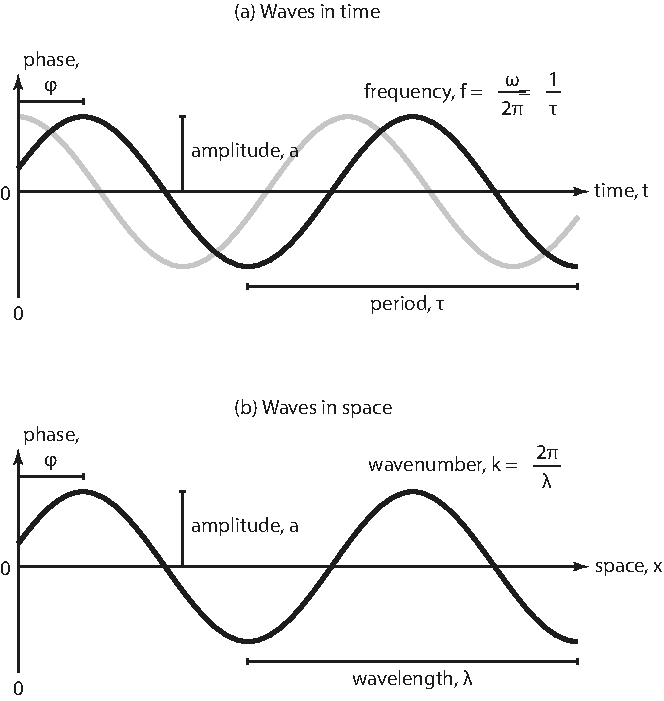
\includegraphics[]{numerical/figures/wave_parameters.pdf}
    \caption{The scale and shifting factors for waves have been given names which differ when describing temporal and spatial signals.  These waves (black) are referenced to a cosine (grey) curve.}
    \label{fig:waveparam}
\end{figure}

The angular frequency $\omega$ is related to the frequency $f$ by
\begin{equation}
    \coreeq
    \omega = 2\pi f,
\end{equation}
where frequency has units of cycles per unit time. The period $\tau$ is the time required for one complete cycle and is given by
\begin{equation}
    \coreeq
    \tau = f^{-1} = \frac{2\pi}{\omega}.
\end{equation}

In geophysics, temporal waves arise naturally in seismology, electromagnetics, and climate records, where periods often correspond to physically meaningful time scales such as wave propagation times, diffusion times, or climatic cycles.

\subsection{Spatial Waves}

An analogous expression describes a wave that varies in space,
\[
    f(t) = \mlbox[
        labelstyle={xshift=-1cm},
        linestyle={out=270,in=90, latex-}]
    {A}{amplitude}
    \cos \bigl(
    \mlbox[
        labelstyle={xshift=-1cm, yshift=-1cm, below of=m\themathLableNode},
        linestyle={out=90,in=270, latex-}]
    {k}{wavenumber}
    \mlbox[
        labelstyle={xshift=0.5cm},
        linestyle={out=270,in=90, latex-}]
    {x}{distance}
    -
    \mlbox[
        labelstyle={xshift=1cm, yshift=-1cm, below of=m\themathLableNode},
        linestyle={out=90,in=270, latex-}]
    {\phi}{phase}
    \bigr),
\]
where the wavenumber $k$ controls the spatial scale of the variation (Figure~\ref{fig:waveparam}). The wavelength $\lambda$ is the distance over which the wave completes a full cycle and is related to wavenumber by
\begin{equation}
    \coreeq
    k = \frac{2\pi}{\lambda}.
\end{equation}

Spatial waves are particularly important in gravity, magnetic, thermal and electromagnetic studies, where wavelength is closely linked to source depth or feature width: long wavelengths are typically associated with deeper sources, while short wavelengths reflect shallow structure.

\subsection{Amplitude, Frequency, and Phase}

Both temporal and spatial waves are fully described by three quantities:
\begin{description}
    \item[Amplitude], which controls the strength of the signal;
    \item[Frequency or wavenumber], which controls the scale of variation;
    \item[Phase], which controls the location of features in time or space.
\end{description}

In temporal problems, frequency is commonly expressed in hertz (cycles per unit time), while in spatial problems the analogous quantity is the wavenumber, which describes cycles per unit distance. The inverse of frequency or wavenumber defines the period or wavelength, quantities that are often more intuitive in a geological context because they correspond directly to time scales or spatial scales of structure.

The phase parameter determines where peaks, troughs, or zero crossings occur. Two waves may have identical amplitude and frequency but differ entirely in appearance due to differences in phase. In geophysics, phase often carries geometric information, such as the location of a source or the alignment of a signal relative to a reference point.

A key observation is that an individual wave, regardless of how finely it is sampled, can be represented exactly using only these three parameters. A time or spatial series containing thousands of sampled values can therefore be compressed into just three numbers if it consists of a single wave. This idea underlies the utility of Fourier methods. Hence, wave descriptions, and Fourier Tranforms, provide a highly compact representation of information.

Most geophysical signals are not composed of a single wave, but rather a superposition of many waves with different frequencies or wavenumbers and phases. The Fourier transform determines these parameters for all constituent waves simultaneously, producing spectra that describe how amplitude and phase vary with scale. For signals dominated by a limited range of scales, this representation can dramatically reduce the complexity of the problem while preserving the essential physical information. Fourier transforms aid identifying dominant frequencies or wavelengths, assessing where noise becomes important, and applying scale-dependent operations (filters) in a controlled and physically interpretable way.


% \section{Introduction}

% In many applications of geophysics we deal with problems where we may know what a function looks like, but not have a mathematical expression to deal with it.
% Examples include
% \begin{enumerate}
%     \item a seismogram, the ground motion (displacement as a function of time) associated with an earthquake;

%     \item a map of the gravity field (or magnetic field, or heat flow, etc.);

%     \item variations in the electric and magnetic field observed at the surface of Earth (magnetotellurics); and

%     \item air temperature changes at the surface of Earth.
% \end{enumerate}
% The first three of the examples relate to temporal variations and one to spatial variations of complex functions that may not be possible to write down as a simple mathematical function.  These problems are not limited to geophysics as they find many applications in other geologic fields as well (particularly, paleoclimate and paleoenvironmental studies).  For example, isotope records in sediment or ice cores can be looked at as a discrete function of that record in time.

% We need to be able to analyze these sorts of data.  Paleoclimate data may be the easiest to consider as an example.  Some major climatic drivers are cyclic including solar energy input (think day/night, yearly variations, and 22 year sunspot cycle), orbital (Milankovitch) cycles (precession, obliquity, and eccentricity of orbit).  For gravity as well as climate, lunar and solar tides are also cyclic.  So for many systems, we may wish to try and find cyclical variations that may otherwise be obscured by additional geological/geophysical processes.

% For spatial variations in potential fields, we are often interested in finding the depth to sources/targets or are interested in isolating near surface versus deep causes.  A problem that also arises with potential fields includes leveling airborne data (gravity, magnetics, radiometrics) flown at different altitudes.

% The analysis required for each of these processes (and many more) require expressing our data as a function.  However, since there is no simple mathematical way to describe our data so we need to develop one.  Fortunately, methods to describe an arbitrary function as a set of simple functions has already been devised.  The most common method utilizes a set of sine and/or cosine functions.  We call this method of constructing arbitrary functions in this way Fourier series.  An extension of the Fourier series is the Fourier transform, which allows us to remove time (or spatial) variables in favor of frequency (or wavenumber) variables, which can make the math far simpler.

% \section{Waves}

% It is possible to write a function as a combination of two or more functions, e.g., $f(x) = g(x) + h(x)$.  What we want to do is write an arbitrary function as a combination of a set of well defined functions.  Ideally, they will share some similar characteristics that will make certain mathematical operations simpler.  A minimal set of parameters is also advantageous, we want our functions to be relatively simple.  Smooth functions are desirable (we can even produce discontinuous functions so long as we use an infinite number of functions).  It is also preferred if our functions are orthogonal and form a basis (see box below).

% The trigonometric functions sine and cosine are ideal candidate functions to build other functions.  First, each function looks relatively similar in form.  Second, one only needs a minimal set of parameters to describe them (amplitude and frequency).  And as will soon see, they form an orthogonal basis.

% Fourier series and Fourier transforms rely on the periodic properties of trigonometric functions and the ease with which they can be scaled and stretched.  A description of the wave parameters are described in 

% We can use these sine and cosine waves to build any function we desire.  An example of a slightly more complex function can be seen in Figure~\ref{fig:cossum}.  The constructed function is a set of 32 cosine functions,
% \begin{equation*}
%     f(x) = \sum_k = 1^32 \cos (k x) .
% \end{equation*}
% While some of the periodicity of the cosines is still evident, it is clear that the function is becoming more and more peaked as terms are added and the amplitude of the ``side lobes'' (the little squiggles about the main peak)
% become smaller.
% \begin{figure}[hbt]
%     \centering
%     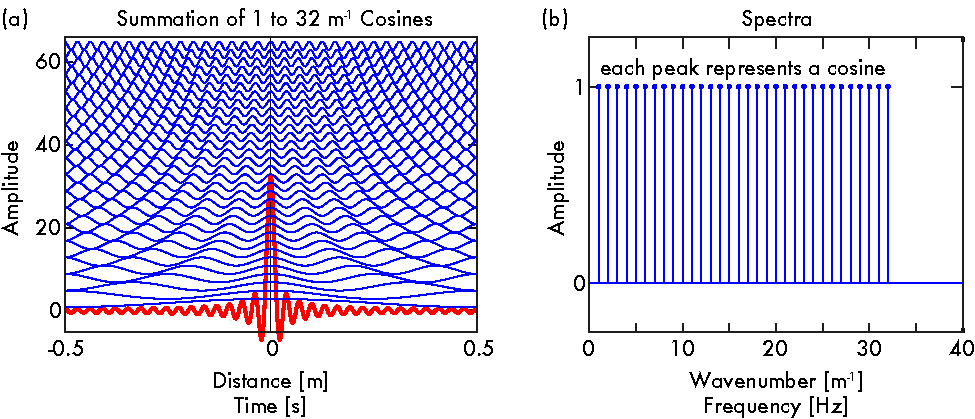
\includegraphics[]{numerical/figures/cosine_sum.pdf}
%     \caption{Demonstrating the construction of a new function using 32 cosine functions. (a) The individual functions in blue are used to construct the function in red. (b) The amplitude spectrum associated with the cosines in (a) showing the frequencies/wavenumbers and their amplitudes (all have the same amplitude).}
%     \label{fig:cossum}
% \end{figure}

\section{Continuous Fourier Transform}

The {\bf continuous Fourier transform} (FT) was first published by Joseph Fourier in 1822 and is used to decompose a function into periodic functions.  FT's find a wide array of uses from identifying the composition of stars (spectroscopy) to cell phone transmissions to image processing to solving differential equations.

Sometimes shorthand notation for a FT is given by 
\[
    h(\xi) \overset{\mcal{F}}{\longleftrightarrow} H(\nu),
\]
where $h(\xi)$ is a function with the FT $H(\nu)$.  Generally, $\xi$ is either time or a spatial coordinate(s) and $\nu$ is the frequency or wavenumber(s) (spatial analog to frequency).  {\bf The forward transform} goes from left to right and {\bf inverse transform} from right to left.

Forward transform
\begin{equation}
    \workeq
    \mcal{F} [h(\xi)] = H(\nu) = 
    \int_{-\infty}^{\infty} h(\xi)
    \exp [ -i 2 \pi (\nu \cdot \xi) ]\, d\xi,
\end{equation}
Inverse transform
\begin{equation}
    \workeq
    \mcal{F}^{-1} [H(\nu)] = h(\xi) = 
    \int_{-\infty}^{\infty} H(\nu)
    \exp [ i 2 \pi (\nu \cdot \xi) ]\, d\nu.
\end{equation}

The complex number $i = \sqrt{-1}$ (Figure!\ref{fig-eipi}).  Note that $j$ is occasionally used as the complex number, particularly in electrical engineering texts.  Recall that $\exp( i \theta ) = \cos(\theta) + i \sin(\theta)$, hence, a FT and its inverse can be represented by a series of trigonometric functions with varying amplitudes and frequencies.
\begin{eqnarray*}
    \exp( i 2 \pi f t ) & = &\cos(2 \pi f t) + i \sin(2 \pi f t) \mbox{ and} \\
    \exp( - i 2 \pi f t ) & = &\cos(2 \pi f t) - i \sin(2 \pi f t).
\end{eqnarray*}

FT's can be performed on temporal (i.e.  {\bf time-domain}) or spatial (i.e.  {\bf spatial-domain}) processes converting a function into the {\bf frequency-domain}.

For example, in two spatial dimensions the Fourier transform is written as
\[
    H(k_x,k_y) = \int_{-\infty}^{\infty}\int_{-\infty}^{\infty}
    h(x,y) \exp [ -i 2 \pi (k_{x}x + k_{y} y) ]\,
    dx\, dy,
\]

\subsection{Interpretation of Variables}

The mathematical form of the Fourier transform does not depend on the physical meaning of the independent variable. The same transform applies whether $\xi$ represents time, space, or another coordinate.

When $\xi = t$, the Fourier transform converts a time-domain signal into a frequency-domain representation, where frequency describes the rate of temporal variation. The inverse of frequency corresponds to a characteristic timescale or period.

When $\xi = x$ (or more generally $\vb{x}$), the Fourier transform converts a spatial signal into a wavenumber-domain representation, where wavenumber describes the rate of spatial variation. The inverse of wavenumber corresponds to wavelength, a directly interpretable measure of spatial scale.

From a geophysical perspective, this distinction is interpretive rather than mathematical. Short periods or wavelengths describe rapid or fine-scale variations, while long periods or wavelengths describe slow or broad-scale structure. In many applications, wavelength is closely related to depth sensitivity, while frequency is linked to timescales of physical processes.

Because the underlying mathematics is identical, Fourier methods provide a unified language for analyzing both temporal and spatial data.

\section{Amplitude and Phase}

A Fourier transform expresses a function as a sum of complex exponentials, each characterized by an amplitude and a phase at a particular frequency or wavenumber. These two quantities describe fundamentally different aspects of a geophysical signal, and it is essential to understand their physical meaning before applying Fourier-domain operations.

A forward Fourier transformed function is complex and therefore can be written as,
\begin{equation}
    H(\nu) = A(\nu) + iB(\nu) = \abs{H(\nu)} \exp [ i \phi(\nu) ],
\end{equation}
where $A(\nu)$ and $B(\nu)$ are the real and imaginary parts of $H(\nu)$, respectively.  We often refer to the {\bf amplitude spectrum}, $\abs{H(\nu)}$, and the {\bf phase spectrum}, $\phi(\nu)$  of a signal.  We can write these two spectra in terms of the real and imaginary parts of $H(\nu)$,
\begin{eqnarray}
    \workeq
    \abs{H(\nu)} & = & [A^{2}(\nu) + B^{2}(\nu)]^{1/2}, \mbox{ and}\\
    \phi(\nu) & = & \tan^{-1}\left[\frac{B(\nu)}{A(\nu)} \right].
\end{eqnarray}is on derivation—focus on interpretation)

In geophysics, Fourier transforms are most often applied to signals or fields that are already known through observation, such as seismograms, gravity and magnetic anomaly maps, or electromagnetic time series. The Fourier domain does not introduce new information; rather, it reorganizes existing information in a way that makes scale-dependent behavior explicit.

In this representation, the \textbf{amplitude} describes how much of a particular frequency or wavelength is present in the signal, while the \textbf{phase} describes where that component is located in time or space. Both are required for a complete description of the original signal.

\subsection{What Amplitude Tells Us}

The amplitude spectrum measures the strength of oscillations at different frequencies or wavenumbers. In spatial problems, it indicates how much variability exists at different length scales; in temporal problems, it shows how energy or variance is distributed across time scales.

Amplitude is often closely tied to physical processes. For example, in potential field data, large amplitudes at long wavelengths are commonly associated with deep or laterally extensive sources, while strong short-wavelength amplitudes suggest shallow structure. In seismic or electromagnetic time series, amplitude spectra can be used to identify dominant frequencies, attenuation effects, or the frequency range over which noise begins to dominate the signal.

Because amplitude reflects the relative importance of different scales, amplitude spectra are widely used for filtering, smoothing, and scale separation.

\subsection{What Phase Tells Us}

Whereas amplitude describes \emph{how much} of each component is present, phase describes \emph{where} it occurs. Phase controls the alignment of peaks, troughs, and zero crossings in time or space and therefore carries information about geometry, location, and waveform shape.

Two signals can have identical amplitude spectra but look entirely different in the time or spatial domain if their phase spectra differ. In geophysical applications, phase often encodes critical information such as the position of sources, the timing of arrivals, or the sharpness of boundaries.

Phase behavior is particularly important in applications such as migration, deconvolution, and reduction-to-the-pole transformations, where the goal is often to relocate or re-center physical features rather than simply emphasize or suppress particular scales.

\subsection{Why Both Amplitude and Phase Matter}

Amplitude and phase together provide a complete description of a Fourier-transformed signal. Amplitude alone describes the distribution of energy or variance across scales, but without phase information it cannot reconstruct the original signal. Phase, in turn, determines the geometric arrangement of those components but does not indicate their relative strength.

This distinction has important practical consequences. Operations that modify only the amplitude spectrum tend to change the smoothness or scale content of a signal while preserving its geometry. Operations that modify phase, by contrast, can shift, distort, or relocate features in time or space, often with significant implications for interpretation.

Understanding the distinct roles of amplitude and phase is therefore crucial for interpreting Fourier-domain results and for anticipating the effects of filtering, continuation, and other spectral operations introduced later in this chapter.


\section{Discrete and Fast Fourier Transforms}

\subsection{Discrete Fourier Transform (DFT)}

Geophysical data are almost always discrete. Measurements are made at specific locations in space or at specific times, with a finite sampling interval and a finite record length. Seismograms are sampled at fixed time steps, gravity and magnetic data are collected at discrete stations or along flight lines, and electromagnetic measurements are recorded at discrete times. As a result, the continuous Fourier transform must be replaced by a discrete formulation when working with real data.

The discrete Fourier transform (DFT) was first developed, although never published, by Heinrich Gauss in 1805 to describe the orbits of asteroids using discrete observations. It was later rediscovered by Cooley and Tukey in 1965 in a form suitable for efficient computation. In most scientific applications, including geophysics, the DFT is far more practical than the continuous Fourier transform because it operates directly on discretely sampled, finite-length data.

\subsubsection*{Finite Sampling and Record Length}

The DFT addresses two fundamental constraints of observed data:
\begin{itemize}
    \item the data are sampled at discrete intervals, and
    \item the data record has finite length.
\end{itemize}

Rather than requiring integration over an infinite domain, the DFT replaces integrals with finite sums and continuous functions with sequences of sampled values.

For a discrete dataset
\[
    \vb{d} = \{d_0, d_1, \ldots, d_{N-1}\},
\]
the DFT produces an equally sized set of complex coefficients,
\[
    \vb{D} = \{D_0, D_1, \ldots, D_{N-1}\},
\]
which describe the contribution of discrete frequencies or wavenumbers to the signal.

\subsubsection*{Definition of the DFT}

The forward discrete Fourier transform is defined as
\begin{equation}
    \workeq
    D_k = \sum_{n=0}^{N-1} d_n 
    \exp \left[-\frac{i 2 \pi}{N} k n\right],
    \quad k = 0, \ldots, N-1,
    \label{eq-dft}
\end{equation}
and the inverse transform as
\begin{equation}
    \workeq
    d_n = \frac{1}{N}\sum_{k=0}^{N-1} D_k 
    \exp \left[\frac{i 2 \pi}{N} k n\right],
    \quad n = 0, \ldots, N-1.
    \label{eq-idft}
\end{equation}

Together, these equations provide a one-to-one mapping between the data sequence and its discrete frequency-domain representation.

Note that within \textsc{Matlab} and many other programming languages, array indices start at 1 rather than 0. In such cases, the sums are written from $1$ to $N$, with the substitutions $n \rightarrow n-1$ and $k \rightarrow k-1$.

\subsubsection*{Discrete Frequencies}

Equations \ref{eq-dft} and \ref{eq-idft} implicitly assume unit sample spacing. To relate the discrete index $k$ to a physical frequency or wavenumber, the sampling interval $\Delta \xi$ must be introduced.

For a record of length $N\Delta \xi$, the discrete frequencies are given by
\begin{equation}
    \workeq
    \nu_k = \frac{k}{N\,\Delta \xi},
    \quad k = 0, \ldots, N-1.
\end{equation}

The sampling rate controls the highest frequency that can be unambiguously represented, which we call the \textbf{Nyquist frequency},
\begin{equation}
    \coreeq
    \nu_{\mathrm{Ny}} = \frac{1}{2\,\Delta \xi}.
\end{equation}
Frequency components higher than the Nyquist frequency cannot be represented correctly and instead are folded back into lower frequencies. This folding is the origin of aliasing and is an unavoidable consequence of undersampling (Section~\ref{sec:aliasing}).

\subsubsection*{Implicit Periodicity}

An important assumption of the DFT is that the discrete data record is treated as one period of a periodic function. In other words, the data sequence is assumed to repeat indefinitely outside the observed interval.

This implicit periodicity can lead to artificial discontinuities at the boundaries of the record, particularly if the first and last samples do not match smoothly. The consequences of this assumption, including spectral leakage and the need for windowing, will be discussed later in the chapter.

\subsubsection*{FFT as a Computational Algorithm}

The fast Fourier transform (FFT) is not a different transform, but an efficient algorithm for computing the DFT. While the direct evaluation of the DFT requires $\mathcal{O}(N^2)$ operations, FFT algorithms reduce the computational cost to $\mathcal{O}(N \log N)$.

Because of this dramatic improvement in efficiency, FFTs make Fourier analysis practical for large geophysical datasets and are the standard method used in modern data processing. Conceptually, however, the FFT produces exactly the same result as the DFT defined in Equations~\ref{eq-dft} and~\ref{eq-idft}.

\subsection{Positive and Negative Frequencies}

Fourier transforms of real-valued data contain both positive and negative frequencies. This feature often causes confusion, but it arises naturally from the mathematical form of the transform rather than from any additional physical signal.

Fourier representation is based on complex exponentials of the form $e^{\pm i2\pi\nu\xi}$. A real sinusoidal function requires both the positive- and negative-frequency exponentials to be represented exactly. As a result, negative frequencies are not independent physical components but are the mathematical counterparts required to construct real-valued signals.

For any real-valued function $f(\xi)$, the Fourier transform satisfies Hermitian symmetry,
\[
F(-\nu) = F^*(\nu),
\]
where $^*$ denotes complex conjugation. Consequently, the amplitude spectrum is symmetric about zero frequency, while the phase spectrum is antisymmetric. All independent spectral information is therefore contained in the positive frequencies.

In geophysical applications, it is common to interpret only the non‑negative frequencies or wavelengths, since negative frequencies do not correspond to additional physical scales. Their presence ensures that inverse transforms return real-valued fields.

Negative frequencies become explicitly important when working with complex-valued signals or phase-sensitive operations, such as analytic signal construction, polarization analysis, or directional wavefield decomposition. Otherwise, they serve primarily as a mathematical requirement of the Fourier representation.

\section{Sampling and Aliasing}\label{sec:aliasing}

\subsection{Consequences of Undersampling}

Geophysical signals are often continuous in time or space, but they must be recorded digitally as a sequence of discrete samples. The sampling interval therefore plays a fundamental role in determining what information can be represented faithfully.

When a signal is undersampled, high-frequency content is misrepresented as lower-frequency content. This distortion is often not obvious and can be difficult to detect because the aliased signal appears internally consistent.

The term \emph{aliasing} comes from the Latin word \emph{alias}, meaning ``otherwise'' or ``at another time,'' and in modern usage often refers to a false or assumed name. In much the same way, aliased frequencies--frequencies \emph{higher} than the Nyquist frequency---masquerade as lower-frequency (longer wavelength) components that were not present in the original signal.

The effects of aliasing are severe and irreversible. Four key consequences are worth emphasizing:
\begin{enumerate}
  \item \textit{``You can't always get what you want.''} Frequency components above the Nyquist frequency are not contained correctly in the sampled data.
  \item \textit{``You get something else instead.''} High-frequency energy appears artificially at lower frequencies, creating spurious signals.
  \item \textit{``You don't know you've made a mistake.''} Aliased data often appear smooth and reasonable, masking the error.
  \item \textit{``It's too late to fix it.''} Once data have been sampled inadequately, the lost information cannot be recovered.
\end{enumerate}

These properties make aliasing particularly dangerous in geophysics, where interpretations often rely on subtle variations in amplitude, frequency content, or spatial scale.  Inadequate sampling leads to aliasing, a serious and often subtle source of error in geophysical analysis.

\subsection{Aliasing Example}

A familiar everyday example is the apparent backward rotation of wheels on a rapidly moving vehicle. As the rotation rate increases, the wheels may appear to slow, stop, or reverse direction. This visual illusion arises because the image is sampled by the human visual system at discrete time intervals, resulting in aliasing. Similar effects can be observed in rotating fan blades or helicopter rotors.

An illustration of aliasing in a sampled time series is shown in Figure~\ref{fig:aliasing}. As the sampling interval becomes too large, the reconstructed signal no longer reflects the true frequency content of the original waveform.

\begin{figure}[hbt]
    \centering
    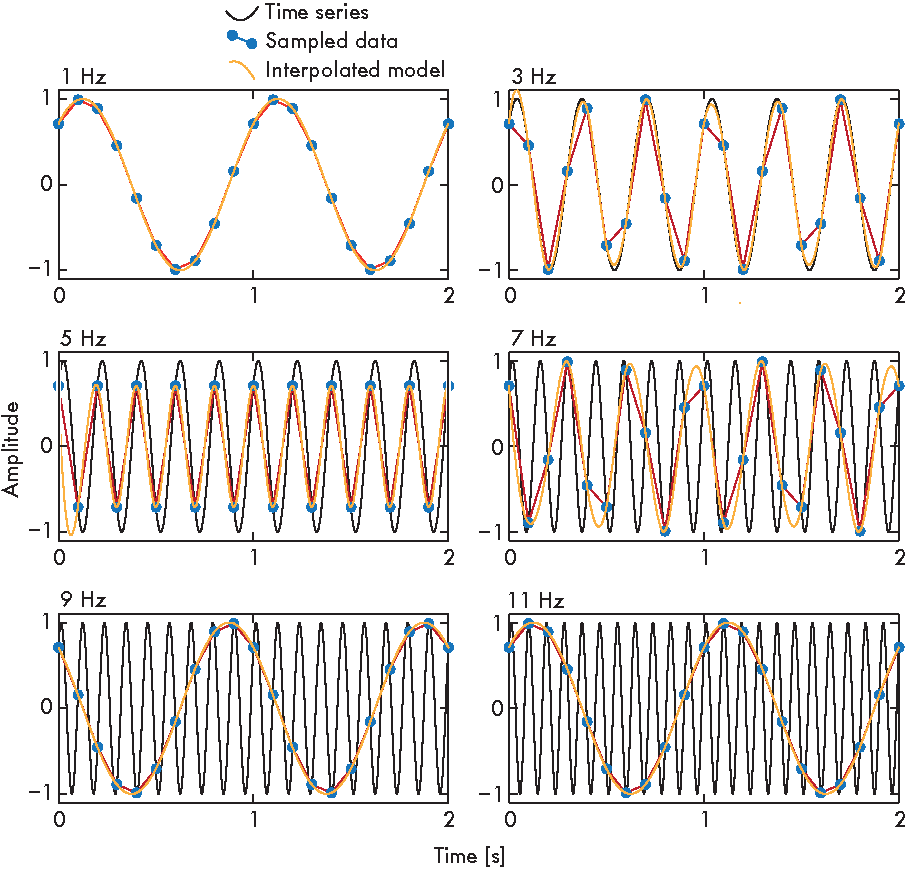
\includegraphics[]{numerical/figures/aliasing.pdf}
    \caption{Demonstration of aliasing. As the frequency of the time series increases and exceeds the Nyquist frequency (5~Hz), the interpolated signal no longer reproduces the original frequency but instead appears as a lower-frequency wave.}
    \label{fig:aliasing}
\end{figure}

\subsection{Nyquist is not enough}

The Nyquist frequency represents a \emph{theoretical} limit, not a guarantee of reliable recovery.  Its derivation assumes exactly periodic sampling, adequate phase coverage, and signal amplitudes that are large compared to noise. In practice, these assumptions are rarely met. Sampling near the nodal points of a waveform can make even sub-Nyquist signals difficult to identify, and phase rapidly becomes under-constrained as one approaches the Nyquist frequency, $\nu_{\mathrm{Ny}}$ (Figure~\ref{fig:nyquist}).

Nyquist therefore defines the maximum frequency that is theoretically representable, not the maximum frequency that can be robustly recovered from data. Near $\nu_{\mathrm{Ny}}$, each cycle is sampled by very few points, such that any pair of samples is nearly equally likely to fall anywhere on the waveform. As a result, small sampling or timing errors can produce large phase errors and a systematic underestimation of amplitude (Figure~\ref{fig:nyquist}b). While amplitude may still be detectable close to the Nyquist frequency, phase information rapidly degrades and becomes effectively meaningless (Figure~\ref{fig:nyquist}c).

In the worst case, sampling occurs exactly at the nodal points of the wave, yielding zero measured amplitude and an apparent phase offset of $180^\circ$ relative to the true signal.  This behaviour is particularly important for traveltime analysis, phase-sensitive inversions, and spectral interpretations in noisy data.

For practical purposes, a more conservative upper limit on usable frequency is often required.  A common rule of thumb is that reliable phase and amplitude recovery typically require at least four samples per cycle (Figure~\ref{fig:nyquist}b, blue line), corresponding to a frequency of approximately
\[
    \nu_{\mathrm{practical}} \approx \frac{1}{4\Delta\xi}.
\]
At this sampling density, a waveform is sufficiently over-resolved that phase estimates are stable against noise, timing errors, and unfavourable sample placement relative to nodal points.  Frequencies between $1/(4\Delta\xi)$ and the Nyquist frequency may be representable in principle, but their interpretation should be treated with caution.
\begin{figure}[htbp]
    \centering
    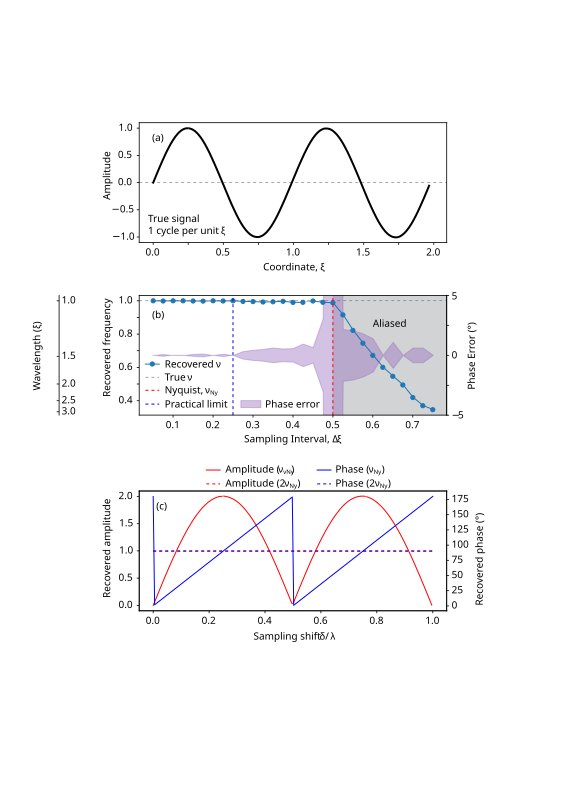
\includegraphics{numerical/figures/nyquist.eps}
    \caption{An exploration of sampling and Fourier transform results around the Nyquist frequency, $\nu_{Ny}$. (a) The true wave, a sinusoid with one cycle per unit coordinate length. Over- and under-sampled waves are shown in blue and red respectively. (b) Recovered frequency relative to sampling frequency.  Sampling intervals larger than the Nyquist alias the signal resulting in incorrect frequency estimates.  Hence under sampled wave in (a) is aliased. Also shown on (b) is the phase error envelope represents the maximum and minimum error possible for a given sampling interval.  The amplitude error is similarly shaped with an amplitude error generally less than 2\%. (c) Sampling at the Nyquist frequency with a shift, $\delta$, of the first sampling point relative to the wavelength, $\lambda$. At the $\nu_{Ny}$, the sinusoidal basis becomes degenerate; amplitude estimates are biased because all energy collapses into a single basis function causing a large error.  Phase estimates are also poor at $\nu_{Ny}$ with potential errors of $\pm90^\circ$.}  
    \label{fig:nyquist}
\end{figure}

\subsection{Preventing Aliasing}

Because aliasing cannot be corrected after sampling, it must be addressed during data acquisition. Two approaches are commonly used:
\begin{enumerate}
  \item \textbf{Survey design.} Anticipate the range of frequencies or wavelengths expected in the signal and choose a sampling interval small enough to exceed the Nyquist requirement.
  \item \textbf{Prefiltering.} If sufficiently high sampling rates are impractical, analog or digital low-pass filters can be applied before digitization to remove frequency components above the Nyquist frequency.
\end{enumerate}

Careful attention to sampling is essential in the design of geophysical surveys and monitoring systems. Many common processing problems, including spurious trends and misleading spectral features, can often be traced back to inadequate sampling at the acquisition stage.


\section{Convolution}

Convolution is a central concept in signal processing and underlies many common operations in geophysics, including filtering, smoothing, instrument response correction, and wavelet modeling. Understanding convolution is essential before introducing Fourier-domain filtering and deconvolution.

\subsection{Definition of Convolution}

Convolution is a mathematical operation that describes how one function modifies another. Given two functions $f(\xi)$ and $g(\xi)$, their convolution is defined as
\begin{equation}
    \coreeq
    (f * g)(\xi) = \int_{-\infty}^{\infty} f(\eta)\, g(\xi - \eta)\, d\eta .
\end{equation}

The value of the convolution at position $\xi$ is obtained by reversing one function, shifting it by $\xi$, multiplying it pointwise with the other function, and integrating the product over the entire domain. The result is a new function that combines the properties of both $f$ and $g$.

\subsection{Physical Meaning of Convolution}

Convolution appears whenever the value of a quantity at a given location or time depends on a weighted combination of nearby values. In geophysics, this situation arises frequently.

Conceptually, $f(\xi)$ represents an input or ideal signal, $g(\xi)$ represents a response function or kernel, and the convolution $f * g$ represents the observed or modified signal. The kernel $g$ determines how information from neighboring points contributes to the value at $\xi$. If $g$ is sharply peaked, the convolution closely resembles the original function. If $g$ is broad, the resulting signal is smoothed over a wider region.

An intuitive interpretation of convolution is as a weighted average. If the kernel $g(\xi)$ is non-negative and normalized such that
\[
    \int_{-\infty}^{\infty} g(\xi)\, d\xi = 1,
\]
then the convolution computes a local average of $f$, weighted according to the shape of $g$.

Different kernels produce different averaging behavior. A Gaussian kernel results in smooth, localized averaging; a boxcar kernel produces a simple running mean; and long-tailed kernels mix information over larger distances or longer times. This interpretation is directly relevant to smoothing, diffusion, and upward continuation in geophysics.

Convolution can also be interpreted as the response of a system to an input. If a system has a characteristic response $g(\xi)$, then convolving that response with an input signal produces the system's output. 

In geophysics, convolution naturally appears in many contexts, including seismic source wavelets modifying reflectivity, instrument responses shaping recorded data, spatial averaging introduced by finite sensor footprints, and diffusion processes spreading localized anomalies. A seismogram (Chapter~\ref{ch:seismology}) is a convolution between the source, its path through Earth, the attenuation and the receiver response function. In each case, convolution describes how structure is transferred across scales. 

\subsection{Convolution in the Fourier Domain}

Direct evaluation of the convolution integral is computationally expensive. For discretely sampled data with $N$ points, a numerical convolution requires $\mathcal{O}(N^2)$ operations, since each output sample depends on contributions from many input samples. This computational burden motivates the use of Fourier transforms, which provide a far more efficient way to evaluate convolutions, $\mathcal{O}(N \log N)$.

A key result of Fourier analysis is the convolution theorem, which states that convolution in the original domain corresponds to multiplication in the Fourier domain. Let
\[
    F(\nu) = \mathcal{F}\{f(\xi)\}, \qquad
    G(\nu) = \mathcal{F}\{g(\xi)\}.
\]
Then,
\[
    \mathcal{F}\{f * g\} = F(\nu)\,G(\nu),
\]
or equivalently,
\[
    f * g = \mathcal{F}^{-1}\!\left\{F(\nu)\,G(\nu)\right\}.
\]

This result is profound: a complicated integral operation in space or time becomes a simple pointwise multiplication in the Fourier domain.

Fourier-domain filtering is simply convolution expressed efficiently. When a filter $H(\nu)$ is applied in the Fourier domain,
\[
    \tilde{F}(\nu) = H(\nu)\,F(\nu),
\]
the corresponding operation in the original domain is convolution,
\[
    \tilde{f}(\xi) = f(\xi) * h(\xi),
\]
where $h(\xi) = \mathcal{F}^{-1}\{H(\nu)\}$ is the filter kernel.

Thus, the shape of the filter in frequency or wavenumber space determines the shape of the convolution kernel in time or space. This dual interpretation is critical for understanding the consequences of filtering.

A central lesson is that sharp spectral filters produce broad, oscillatory kernels, while smooth spectral filters produce compact, localized kernels. For example, an ideal low-pass filter with an abrupt cutoff yields a kernel that oscillates indefinitely in the original domain, whereas a Gaussian low-pass filter produces a smoothly decaying kernel.

This relationship explains why abrupt spectral truncation leads to ringing and overshoot near discontinuities. Such effects are not numerical artifacts, but a direct and predictable consequence of convolution with a long-range oscillatory kernel.

Fourier transforms do not alter the physical meaning of convolution; they simplify its execution and interpretation. By working in the Fourier domain, convolution becomes multiplication, scale dependence becomes explicit, filtering operations become computationally efficient, and issues of stability and noise amplification can be assessed algebraically.

For these reasons, Fourier transforms are indispensable tools for understanding and applying convolution-based operations throughout geophysics.


\section{Filtering}

Fourier transforms allow many common operations on geophysical data to be performed efficiently by modifying the amplitude and/or phase spectra. Working in the Fourier domain often simplifies these operations, turning convolution, differentiation, and filtering into algebraic manipulations. However, not all Fourier-domain operations affect data in the same way.

It is essential to distinguish between \textbf{amplitude filters}, which modify the relative importance of different scales, and \textbf{phase filters}, which alter the spatial or temporal alignment of features. These two classes of operations have very different physical consequences and must be interpreted with care.

\subsection{Amplitude Filters (Scale-Selective Operations)}

Amplitude filters modify how much of each frequency or wavelength contributes to the signal, while leaving the phase unchanged. Because phase controls geometry, amplitude-only filtering preserves the spatial or temporal arrangement of features but changes the smoothness or resolution of the data.
\[
    H(\nu) = A(\nu),
\]

Amplitude filters operate by altering the magnitude spectrum of a Fourier-transformed signal. Long-wavelength components can be emphasized or suppressed independently of short-wavelength components, making these filters relatively straightforward to interpret physically.

An ideal low-pass filter can be defined as
\[
    H(\nu) =
    \begin{cases}
        1, & |\nu| \le \nu_c, \\
        0, & |\nu| > \nu_c,
    \end{cases}
\]
but such filters are rarely used in practice.

The discontinuity in $H(\nu)$ introduces oscillatory behavior in the filtered signal near sharp transitions. These oscillations are a manifestation of the Gibbs phenomenon, which arises whenever sharp spectral cutoffs are applied to signals with discontinuities or strong gradients.

Common amplitude filters include low-pass filters, which emphasize long wavelengths and suppress short wavelengths; high-pass filters, which do the opposite; and band-pass or band-stop filters, which isolate or remove specific ranges of scale. Spectral smoothing and tapering in frequency or wavenumber space are also amplitude-filtering operations.  Figure~\ref{fig:filtering} illustrates the basic idea. 
\begin{figure}[hbt]
    \centering
    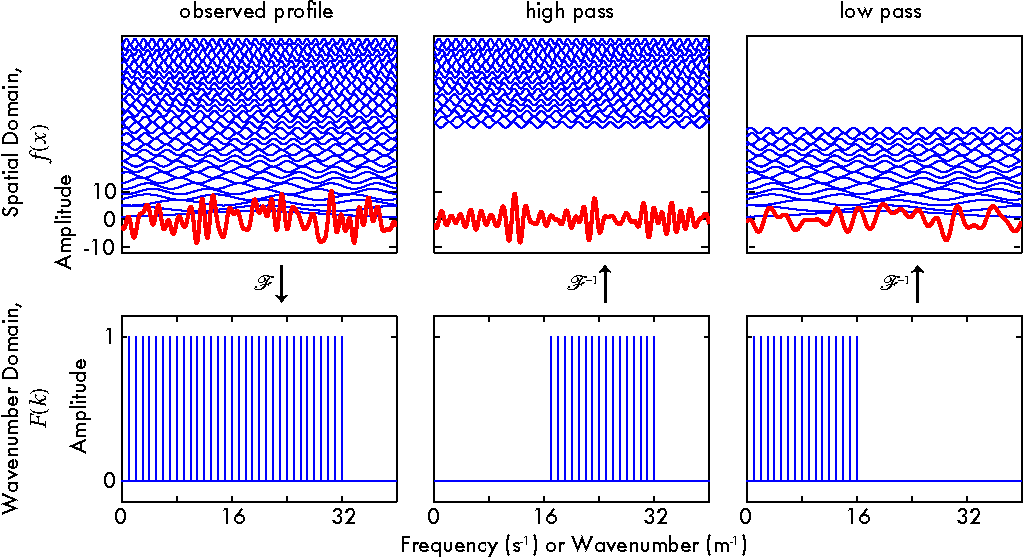
\includegraphics[]{numerical/figures/filtering.pdf}
    \caption{Use of Fourier transforms to filter a time series. The original signal can be separated by frequency or wavenumber to examine short- and long-period components individually.}
    \label{fig:filtering}
\end{figure}

In geophysical applications, amplitude filters are often used to separate regional and residual gravity fields, distinguish shallow from deep magnetic sources, reduce noise in seismic or magnetotelluric data, or emphasize characteristic length scales associated with geological structure.

Despite their apparent simplicity, amplitude filters must be applied cautiously. Filtering irreversibly removes information, and overly aggressive filtering may eliminate physically meaningful signals. The shape of the filter response is also important: sharp cutoffs can introduce artifacts, while smoother roll-offs generally produce more stable results.
\[
    A(\nu) = \exp\!\left(-\frac{\nu^2}{\nu_c^2}\right)
\]

\[
    A(\nu) =
    \exp\!\left[-\frac{(\nu-\nu_0)^2}{\sigma^2}\right]
\]
\[
    \arg\bigl(\tilde{F}(\nu)\bigr)=\arg\bigl(F(\nu)\bigr),
\]

\subsection{Phase and Mixed Filters (Geometry-Altering Operations)}

Phase filters modify where features appear in time or space and therefore directly affect geological interpretation. Unlike amplitude filters, phase-altering operations do not merely change the relative contribution of scales, but can shift, distort, or relocate physical features.
\[
    H(\nu) = e^{i\phi(\nu)}.
\]

Operations that modify phase may act on the phase spectrum alone or may affect both phase and amplitude simultaneously. Because phase carries information about geometry and position, these filters are often more sensitive to noise and to assumptions built into the processing method.
\[
    H(\nu) = e^{-i2\pi\nu\xi_0}
\]

Examples of phase-altering or mixed filters include time or space shifts, the Hilbert transform, construction of the analytic signal, reduction to the pole in magnetic interpretation, deconvolution in seismology, and migration-type operations. In each case, the goal is not simply to emphasize certain scales, but to change how features are positioned or expressed in the data.
\[
    \tilde{f}(\xi) = f(\xi-\xi_0).
\]

Phase filters are powerful but potentially hazardous. Small phase errors can produce misleading structures, particularly at short wavelengths where noise often dominates. The stability of phase-based operations is therefore strongly dependent on data quality and on the validity of the underlying physical assumptions.

\subsection{Operations Combining Amplitude and Phase}

Many practical Fourier-domain methods unavoidably modify both amplitude and phase. Examples include upward and downward continuation, derivative operators such as gradients and Laplacians, inverse filtering, and some spectral methods for estimating source depth.

\subsubsection{Upward and downward continuation}\label{sec:continuation}

Continuation is a fundamental operation in potential field geophysics that allows the field to be evaluated at a different elevation than where it was measured. Physically, this corresponds to predicting how the field would change if the observation surface were moved upward or downward.

For potential fields such as gravity and magnetics, the field satisfies Laplace's equation in source-free regions. This property allows continuation to be expressed conveniently in the Fourier domain.

If a field is known on a horizontal surface, its upward continuation by a height $h$ is given in the Fourier domain by
\[
    H(\mathbf{k}) = e^{-|\mathbf{k}|h},
\]
\[
    \tilde{F}(\mathbf{k}) = F(\mathbf{k})\, e^{-|\mathbf{k}|h},
\]
where $\mathbf{k}$ is the wavenumber vector and $|\mathbf{k}|$ represents spatial frequency.

This expression shows that upward continuation acts as a low-pass filter:
\begin{itemize}
    \item high-wavenumber (short-wavelength) components decay rapidly,
    \item low-wavenumber (long-wavelength) components are preserved.
\end{itemize}

Geophysically, this reflects the fact that short-wavelength anomalies are produced by shallow sources, which decay rapidly with distance. Upward continuation therefore smooths the field and emphasizes deeper, regional structure.

In contrast, downward continuation is given by
\[
    H(\mathbf{k}) = e^{+|\mathbf{k}|h},
\]
which amplifies high-wavenumber components.

This has the opposite effect:
\begin{itemize}
    \item enhances short-wavelength anomalies,
    \item increases apparent resolution of shallow features.
\end{itemize}

However, downward continuation is inherently unstable because it amplifies not only signal but also noise. Even small amounts of high-frequency noise can grow rapidly, limiting the practical depth to which data can be continued downward.

\subsubsection{Relationship to derivatives}

Derivative operators are closely related to continuation. For example,
\[
    \mathcal{F}\left\{\frac{df}{dx}\right\}
    = i 2 \pi k\,F(k),
\]
showing that differentiation increases the contribution of high-wavenumber components.

This means that:
\begin{itemize}
    \item derivatives enhance sharp features,
    \item but also amplify noise.
\end{itemize}

Like downward continuation, derivative operators trade stability for resolution.

\subsubsection{Practical considerations}

Continuation and derivative operations are widely used in both gravity and magnetic data processing and can be found in geothermics. However, their usefulness is controlled by the balance between signal enhancement and noise amplification.

In practice:
\begin{itemize}
    \item upward continuation is stable and commonly used to isolate regional fields,
    \item downward continuation is limited by noise and requires regularization,
    \item derivative-based filters must be applied with care.
\end{itemize}

These operations are used extensively in the separation of regional and residual fields and in spectral interpretation methods.

\emph{Key idea:} Continuation exploits the physics of potential fields to redistribute energy between spatial scales. Upward continuation suppresses shallow sources and stabilizes the field, while downward continuation enhances resolution but amplifies noise.

\subsection{Physical Interpretation and Best Practices}

Amplitude filters primarily control scale and are often interpretable in terms of depth sensitivity or smoothing. Phase filters, by contrast, control geometry and require stronger physical assumptions about the data and the sources that produced them.

When applying any Fourier-domain operation, it is good practice to ask:
\begin{itemize}
    \item What information am I suppressing or amplifying?
    \item What physical or mathematical assumptions am I imposing?
    \item Is the operation reversible, or does it permanently alter the data?
\end{itemize}

Clear answers to these questions are essential for responsible interpretation.

\subsection{Preview of Field-Specific Applications}

The concepts introduced here appear throughout geophysics. In gravity and magnetics, Fourier-domain operations underpin continuation and reduction-to-the-pole methods. In seismology, amplitude and phase manipulation form the basis of deconvolution and wavelet correction. In magnetotellurics, frequency-dependent response functions and coherence analysis rely directly on Fourier-domain representations.

Understanding how amplitude and phase are modified in these operations provides a unifying perspective that are developed further in previous chapters.

\section{Deconvolution}

If convolution describes how a signal is modified by a system or filter, deconvolution attempts to undo that modification by estimating the original signal from the observed one. If an observed signal $d(\xi)$ is related to a true signal $f(\xi)$ through convolution with a kernel $g(\xi)$,
\[
    d(\xi) = f(\xi) * g(\xi),
\]
then deconvolution seeks an estimate $\hat{f}(\xi)$ such that
\[
    \hat{f}(\xi) * g(\xi) \approx d(\xi).
\]
Unlike convolution, which is always well defined, deconvolution is an inverse problem and may not have a unique or stable solution.

Like convolution, deconvolution is most naturally performed in the Fourier domain. Using the convolution theorem,
\[
    D(\nu) = F(\nu)\,G(\nu),
\]
where $D$, $F$, and $G$ are the Fourier transform of $d$, $f$, and $g$, respectively. A formal deconvolution would take the form
\[
    \hat{F}(\nu) = \frac{D(\nu)}{G(\nu)}.
\]
The appearance of division marks a fundamental difference between convolution and deconvolution. It is this division that introduces both power and danger.

Deconvolution differs from convolution because it is sensitive to small values of $G(\nu)$ and strongly amplifies noise. If $G(\nu)$ is small or zero at some frequencies, then
\[
    \frac{D(\nu)}{G(\nu)}
\]
becomes very large or undefined. In practice, many physical systems strongly suppress certain frequencies, making exact inversion impossible. Frequencies that are weak or absent after convolution therefore cannot be reliably recovered by deconvolution.

Observed data always contain noise,
\[
    D(\nu) = F(\nu)\,G(\nu) + N(\nu).
\]
Deconvolution then produces
\[
    \hat{F}(\nu) = \frac{F(\nu)\,G(\nu)}{G(\nu)} + \frac{N(\nu)}{G(\nu)}
                = F(\nu) + \frac{N(\nu)}{G(\nu)}.
\]
Where $G(\nu)$ is small, noise is strongly amplified and may dominate the result. This is why deconvolution is typically unstable at high frequencies or short wavelengths.

Loss of information during convolution is irreversible. Convolution often removes information through smoothing or attenuation, and deconvolution cannot restore information that is no longer present in the data. This limitation contrasts sharply with convolution, which always produces a valid output from a valid input.

\subsection{Regularized Deconvolution}

Because of these issues, practical deconvolution is never implemented as simple division. Instead, regularization is introduced to stabilize the solution. A commonly used form is
\[
    \hat{F}(\nu) = \frac{G^*(\nu)}{|G(\nu)|^2 + \epsilon}\,D(\nu),
\]
where $G^*(\nu)$ is the complex conjugate of $G(\nu)$ and $\epsilon$ is a stabilizing parameter.

Regularization prevents uncontrolled growth where $G(\nu)$ is small, at the cost of incomplete inversion. The trade-off is unavoidable: increased stability reduces resolution, while increased resolution amplifies noise.

\subsection{Physical Interpretation}

Physically, convolution describes how energy or information spreads, smooths, or is redistributed. Deconvolution attempts to reverse that spreading under imperfect conditions. Examples in geophysics include removing seismic source wavelets, correcting instrument response, sharpening blurred reflectors, and compensating for attenuation.

In all cases, the effectiveness of deconvolution depends on how accurately the kernel $g(\xi)$ is known, how much information survived convolution, and how noise is distributed across frequency.

\begin{table}[hbt]
    \centering
    \caption{Contrasting convolution and deconvolution.}
    \label{tab:convolution}
    \begin{tabular}{@{}lll@{}}
        \toprule
        Aspect & Convolution & Deconvolution \\
        \midrule
        Mathematical operation & Multiplication in Fourier domain & Division in Fourier domain \\
        Stability & Always stable & Potentially unstable \\
        Noise behavior & Often suppresses noise & Often amplifies noise \\
        Information flow & Loses or redistributes information & Cannot recover lost information \\
        Physical role & Forward modeling / filtering & Inverse estimation \\
        \bottomrule
    \end{tabular}
\end{table}

\subsection{Why Fourier Transforms Are Critical for Deconvolution}

Without Fourier transforms, deconvolution is impractical. Division in the Fourier domain replaces integral equations in the original domain, making frequency-dependent stability explicit. Regularization strategies can be designed directly by scale. Fourier transforms do not make deconvolution easy, but they make its limitations explicit, which is essential for responsible interpretation.

\section{Interpretation and Pitfalls}

Fourier methods provide a powerful framework for analyzing and manipulating geophysical data, but they must be used with care. The Fourier domain makes certain properties of a signal explicit—particularly scale and frequency content—but it also obscures others, such as localization in space or time. As a result, Fourier-based analysis introduces important limitations and potential pitfalls that must be understood to avoid misinterpretation.

\subsection{Resolution Limits}

A fundamental limitation of Fourier methods is that resolution is constrained by the length and spacing of the data record. Finite sampling intervals limit the highest frequency or shortest wavelength that can be resolved, while finite record length limits the resolution at low frequencies or long wavelengths.

In practice, this means that closely spaced features may not be distinguishable if they correspond to frequencies above the Nyquist limit, and long-wavelength phenomena may be poorly resolved if the data window is too short. These limitations are not shortcomings of the Fourier transform itself, but reflect the finite information content of the data.

In geophysical terms, resolution limits often translate into depth limitations. Short-wavelength features associated with shallow structure may be unresolved in coarse surveys, while long-wavelength signals associated with deep structure may be poorly constrained by limited survey extent.

\subsection{Noise Amplification}

Fourier-domain operations inevitably interact with noise. While some operations, such as low-pass filtering, tend to suppress high-frequency noise, others—particularly inverse operations—can dramatically amplify it.

Noise amplification is most pronounced when filters increase the relative weight of frequencies where the signal-to-noise ratio is low. This is especially evident in deconvolution and downward continuation, where division by small spectral values amplifies noise and numerical errors. In such cases, high-frequency components may become dominated by noise, leading to unstable or misleading results.

Recognizing when an apparent feature is noise-driven rather than physically meaningful is a critical component of responsible interpretation. Noise amplification is not a numerical artifact but a predictable mathematical consequence of the operation being applied.

\subsection{Edge Effects and Windowing}

Fourier transforms implicitly assume that a finite data record represents one period of a periodic function. When this assumption is violated—as it almost always is in real geophysical data—discontinuities arise at the edges of the record. These discontinuities introduce artificial high-frequency components that can contaminate the spectrum.

Edge effects are particularly problematic when applying sharp spectral filters or computing derivatives in the Fourier domain. One common mitigation strategy is windowing, in which the data are smoothly tapered to zero at the boundaries before transformation. Windowing reduces artificial discontinuities but also modifies the spectral content of the data, introducing a trade-off between edge suppression and spectral resolution.

Because windowing itself is a form of convolution, it must be interpreted as an intentional modification of the data rather than a benign preprocessing step.

\subsection{Physical and Non-Physical Spectral Features}

Not all features observed in the Fourier domain correspond to real physical processes. Some spectral peaks arise from periodic sampling, survey geometry, or processing choices rather than from geology or geophysics. Others may reflect mathematical consequences of filtering, truncation, or windowing.

Distinguishing physical from non-physical spectral features requires careful consideration of acquisition geometry, sampling rates, and processing history. In particular, sharp cutoffs, periodic gaps in data coverage, and aggressive filtering can all introduce spectral artifacts that resemble genuine signals.

A useful interpretive question to ask is whether a feature persists under reasonable changes in processing parameters. Physically meaningful features are generally robust, while artifacts often change or disappear when filters, windows, or sampling assumptions are modified.

\subsection{Summary of Best Practices}

Fourier-domain methods are powerful precisely because they reorganize data in a way that highlights scale-dependent behavior. At the same time, they impose assumptions and limitations that must be acknowledged explicitly. When working in the Fourier domain, it is good practice to:
\begin{itemize}
    \item relate spectral features back to physically plausible length or time scales,
    \item assess sensitivity to noise and sampling limitations,
    \item examine the effects of edges and windowing,
    \item and interpret spectral structure in the context of acquisition and processing choices.
\end{itemize}

A clear understanding of these issues allows Fourier methods to be used as effective interpretive tools rather than black-box procedures.

% \section{Geophysical Applications}

% \begin{itemize}
%     \item Gravity and magnetic field analysis
%     \item Seismic signal processing
%     \item MT time-series analysis
%     \item Climate and paleo records
% \end{itemize}

\section{Summary and Forward Links}

Fourier transforms provide a powerful framework for analyzing geophysical data by reorganizing information according to frequency or wavelength. Rather than solving for unknown fields, as in the case of Fourier series, Fourier transforms operate on known data and make scale-dependent behavior explicit.

Throughout this chapter, we have emphasized that Fourier transforms are best understood as tools for interpreting and manipulating data rather than as physical models. In the Fourier domain, operations such as filtering, continuation, differentiation, and deconvolution become algebraically simple, and their effects on scale, geometry, and stability can be assessed directly.

A central theme has been the distinction between forward and inverse operations. Filtering and upward continuation represent stable, forward applications of convolution, while deconvolution and downward continuation are inverse problems that are inherently sensitive to noise and require regularization. Understanding this distinction is essential for responsible interpretation of Fourier-domain results.

The concepts developed here recur throughout geophysics. In potential field methods, Fourier transforms underpin continuation and spectral techniques for depth estimation. In seismology, they form the foundation of signal processing and wavefield manipulation. In electromagnetic methods, Fourier analysis links time-domain observations to frequency-dependent Earth response.

It is worth contrasting these ideas with those introduced in the previous chapter on Fourier series. Fourier series arise naturally when solving boundary-value problems on finite domains and are driven by the physics and boundary conditions of the system. Fourier transforms, by contrast, are analysis tools applied to observed data, where the domain is effectively unbounded and the goal is interpretation rather than construction of a solution.

Recognizing this distinction—and how the two approaches complement one another—provides a coherent framework for understanding why Fourier methods appear so widely across geophysics and how they should be applied in different contexts.
\chapter{Finite Differences} \label{ch:finitediff}

\epigraph{``Our goal should be to understand our differences.''}
{{\normalfont ---\ James D. Watson}}

\section{Introduction}
Most geophysical fields are governed by partial differential equations that express conservation of mass, energy, or momentum. In earlier chapters, we developed these equations analytically and explored their physical meaning through idealized geometries and closed-form solutions. Those analytic solutions are indispensable for building intuition, but they are also limited. Real geologic systems rarely conform to simple geometries, constant material properties, or uniform boundary conditions. At some point, the Earth becomes too complicated to solve with pencil and paper.

\textbf{Finite difference methods} provide a bridge between the governing equations of geophysics and the complexity of real Earth systems. Rather than attempting to solve a partial differential equation everywhere at once, we approximate it by enforcing its local balance on a discrete grid in space and time. In doing so, we \emph{replace continuous derivatives with differences between neighboring points}, turning differential equations into algebraic ones that can be solved on a computer.

Although finite difference methods are often introduced as numerical tools, their deeper significance is physical rather than computational. Each finite difference approximation represents a local statement of conservation. For example, the second spatial derivative in a diffusion equation measures local curvature of a field; in discrete form, it compares the value at one point to the average of its neighbors. Diffusion, whether of heat, chemical species, or electric current, becomes a process of local balancing repeated across the domain.

Throughout this chapter we use temperature as a unifying example, drawing on geothermics to illustrate both steady-state and time-dependent behavior. This choice is not restrictive. The same finite difference formulations apply to gravitational and electric potentials, chemical concentration, groundwater head, and displacement fields. Temperature provides a familiar and physically intuitive context in which gradients, curvature, boundary conditions, and time dependence can be understood concretely.

A central theme of this chapter is that the behavior of finite difference solutions depends fundamentally on the type of partial differential equation being solved. Elliptic equations, such as Poisson's and Laplace's equations for steady-state heat conduction or gravity, lead to systems of algebraic equations that enforce instantaneous balance throughout the domain. Parabolic equations, such as the heat diffusion equation, introduce storage and time dependence, requiring solutions to be advanced incrementally in time and giving rise to stability constraints and characteristic diffusion timescales. Hyperbolic equations, which govern wave propagation, impose entirely different numerical constraints related to causality and finite propagation speed.

Understanding these distinctions is essential. Finite difference methods do not merely approximate derivatives; they encode the physics of how information, energy, or mass moves through the Earth. Choices about grid spacing, time step, and boundary conditions are therefore not purely numerical decisions. They reflect assumptions about scales, processes, and the physical regime in which a model is valid.

This chapter introduces finite difference methods with three goals. First, to show how spatial and temporal derivatives are approximated in a way that respects the underlying conservation laws. Second, to connect numerical behavior directly to the elliptic, parabolic, and hyperbolic nature of geophysical equations. Third, to provide a foundation for forward modeling and inversion in later chapters, where numerical solutions become unavoidable.

By the end of this chapter, finite differences should no longer appear as a black-box numerical technique, but as a natural and physically transparent extension of the governing equations that underlie all of geophysics. Whether or not you pursue a career in geophysics, finite difference methods are widely used across science and engineering wherever spatial and temporal processes are governed by partial differential equations.

\subsection{Lithospheric Temperatures: A Unifying Example}

Before introducing the mechanics of finite difference approximations, it is useful to anchor the discussion in equations that are already familiar.  Throughout earlier chapters, we encountered a small number of governing equations that recur across geophysics, differing not in form but in physical fields and properties.

Here we return to those equations using temperature as a unifying example.  Our goal is not to derive them again, but to show how the same mathematical structure leads to very different numerical behavior once the equations are discretized in space and time.

Let the temperature field be
\[
T = T(\vb{x},t),
\]
governed by one of the following PDEs:

\begin{itemize}
  \item \textbf{Elliptic (steady state heat conduction):}
  \[
  \nabla^2 T = -\frac{A}{k},
  \]
  where $A$ is internal heat production and $k$ is thermal conductivity.

  \item \textbf{Parabolic (heat diffusion):}
  \[
  \frac{\partial T}{\partial t} = \kappa \nabla^2 T,
  \]
  where $\kappa = k/(\rho c_p)$ is thermal diffusivity.

  \item \textbf{Hyperbolic (waves, later chapters):}
  \[
  \frac{\partial^2 T}{\partial t^2} = c^2 \nabla^2 T.
  \]
\end{itemize}

The finite difference methods developed here are identical in spirit for all three cases; what differs is how information propagates through the domain.

Before discretizing these equations, it is useful to visualize the physical system they describe Figure~\ref{fig:xseciton}.

\begin{figure}
    \centering
    %\includegraphics[]{numerical/figures/.eps}
    \caption{A geologic cross-section of ???.  The model suggests smoothly varying layer interfaces with the occasional step from a fault. Each rock unit is assumed homogenous with a unique set of physical properties that describes it. This model will form the basis for developing the discrete grid for finite difference modelling.}
    \label{ref:xsection}
\end{figure}


\section{From Continuous Derivatives to Discrete Differences}

\subsection{Taylor Series Expansion: Local Approximation}

Finite difference methods rely on a simple but powerful mathematical idea: a smooth function can be represented locally by a polynomial whose coefficients are determined by its derivatives at a point.  Finite difference approximations are built on Taylor series expansions.  Although Taylor series are often introduced in mathematics courses, many students may not have seen them recently, so we briefly summarize their role here.

A Taylor series provides a local representation of a function in the neighborhood of a point. It expresses the value of a function at nearby locations in terms of its value and derivatives evaluated at a single point.  In essence, a Taylor series answers the question: if we know how a function behaves at one location, how well can we predict its behavior a short distance away?

Taylor series are especially useful in numerical methods because they provide a systematic way to relate derivatives to differences between values at nearby points. Truncating a Taylor series after a finite number of terms produces an approximation whose accuracy depends on the spacing between points. This truncation is the origin of discretization error in finite difference methods.

Let $f(x)$ be a sufficiently smooth scalar field. The Taylor series expansion
of $f$ about the point $x_i$ expresses the value of the function nearby as
\[
f(x_i + \Delta x)
=
f(x_i)
+ \Delta x \eval{\dv{f}{x}}_{x=x_i}
+ \frac{\Delta x^2}{2!} \eval{\dv[2]{f}{x}}_{x=x_i}
+ \frac{\Delta x^3}{3!} \eval{\dv[3]{f}{x}}_{x=x_i}
+ \cdots ,
\]
where $!$ indicates a factorial ($n! = \prod_{i=1}^n i$) and the ellipsis indicates higher-order derivative terms.

This expansion is not an approximation; it is an exact representation of the function provided all terms are retained. In practice, however, we truncate the series after a finite number of terms. Doing so converts the series into an approximation whose accuracy depends on both the spacing $\Delta x$ and the order at which the series is truncated.

Taylor series are useful because they allow derivatives to be related to differences between function values at nearby points. This makes them the natural mathematical foundation for finite difference methods, which replace continuous derivatives with discrete approximations on a grid.

In the discussion that follows, the function $f(x)$ represents a generic scalar field. For most of this chapter, we will use $T$ rather than $f$, but the same approximations apply equally to other geophysical fields such as gravitational potential, electric potential, chemical concentration, or displacement.

\subsection{Approximating derivatives}
\subsubsection{First-Order derivatives}

Finite difference approximations arise naturally from Taylor series
expansions. This connection is important because it makes explicit that
numerical derivatives are not exact, but controlled approximations with
well-defined error.

Consider a smooth function $f(x)$ expanded about the point $x_i$.  We can approximate the first derivative ($\eval{\dv{f}{x}}_{x=x_i}$) using the Taylor Series expansion as either a forward difference,
\begin{equation}
    f(x_i + \Delta x) \approx
    f(x_i)
    + \Delta x \eval{\dv{f}{x}}_{x_i}
    + \frac{\Delta x^2}{2!} \eval{\dv[2]{f}{x}}_{x_i}
    + \frac{\Delta x^3}{3!} \eval{\dv[3]{f}{x}}_{x_i}
    + \cdots,
    \label{eq:ftaylor}
\end{equation}
or a backward difference,
\begin{equation}
    f(x_i - \Delta x) \approx
    f(x_i)
    - \Delta x \eval{\dv{T}{x}}_{x_i}
    + \frac{\Delta x^2}{2!} \eval{\dv[2]{f}{x}}_{x_i}
    - \frac{\Delta x^3}{3!} \eval{\dv[3]{f}{x}}_{x_i}
    + \cdots.
    \label{eq:btaylor}
\end{equation}
Note the difference in signs between the two cases.

Truncation converts an exact representation into an approximation, and the omitted terms define the error introduced by the approximation. Retaining fewer terms leads to larger errors, while retaining more terms improves accuracy at the cost of additional complexity.  If we retain only the first derivative term in the forward expansion and neglect all higher-order terms, after rearranging to isolate for the derivative we obtain 
\begin{equation}
    \coreeq
    \text{Forward difference:}\quad
    \eval{\dv{f}{x}}_{x_i} \approx \frac{f(x_i + \Delta x) - f(x_i)}{\Delta x}.
    \label{eq:ffd}
\end{equation}
This forward difference approximation estimates the derivative at $x_i$ using information from the point ahead of it (Figure~\ref{fig:fddiscrete}). Because it is based on a one-sided expansion, the neglected higher-order terms introduce a systematic error.  Similarly, truncating the backward expansion after the first derivative term yields
\begin{equation}
    \coreeq
    \text{Backward difference:}\quad
    \eval{\dv{f}{x}}_{x_i} \approx \frac{f(x_i) - f(x_i - \Delta x)}{\Delta x}.
    \label{eq:bfd}
\end{equation}
This backward difference approximation uses information from the point behind $x_i$ (Figure~\ref{fig:fddiscrete}) and introduces a different truncation error of comparable magnitude.  Both forward and backward differences are first-order accurate, meaning that their leading error term scales linearly with the grid spacing $\Delta x$.
\begin{figure}[bth]
    \centering
    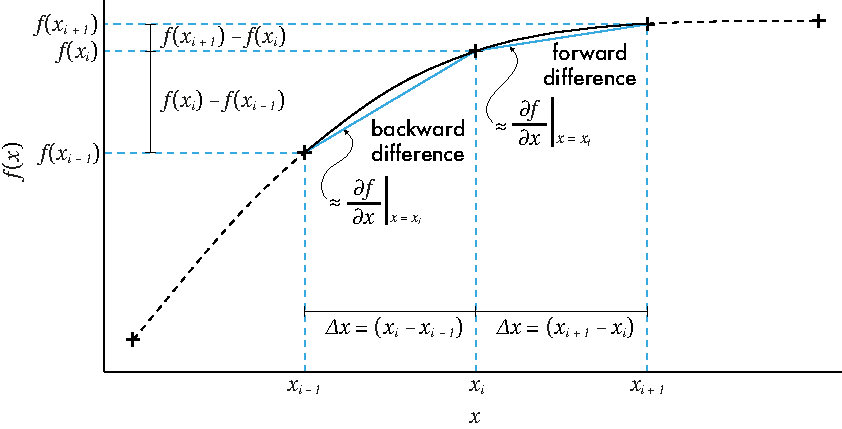
\includegraphics[]{numerical/figures/fddiscrete.pdf}
    \caption{Formulation of finite differences by discretizing a function.  The backward and forward differences are identified by the line segments between the nodes preceding and succeeding $z_i$, respectively.}
    \label{fig:fddiscrete}
\end{figure}

A more accurate approximation can be obtained by taking the arithmetic mean of the forward and backward differences. If we add the forward and backward Taylor expansions (Equations:~\ref{eq:ftaylor} and~\ref{eq:btaylor}) and divide by $2\Delta x$, the odd-order derivative terms cancel, yielding a symmetric approximation.  After solving for the derivative,
\begin{equation}
    \coreeq
    \text{Central difference}\quad
    \eval{\dv{f}{x}}_{x_i} \approx \frac{f(x_i + \Delta x) - f(x_i - \Delta x)}{2\Delta x}.
    \label{eq:cfd}
\end{equation}
This is known as the \emph{central difference} approximation. Because the leading-order asymmetric error terms cancel, the central difference is second-order accurate: its leading truncation error scales with $\Delta x^2$.  This cancellation illustrates two important principles in numerical methods:
\begin{itemize}
    \item symmetry improves accuracy---central differences use information from both sides of a point and therefore provide a better local approximation to the derivative than one-sided schemes; and
    \item finite difference methods do not eliminate error, they control it---the choice of grid spacing determines the magnitude of truncation error, while the choice of time step and scheme determines how that error propagates through a solution.
\end{itemize}

Central differences are preferred throughout most of a numerical domain. However, near boundaries, where information from one side of a node is unavailable, we are often forced to use forward or backward differences. The treatment of such boundary regions is discussed later when we consider discretized domains and boundary conditions.

\subsubsection{Second-Order Derivatives}

Many of the governing equations encountered in geophysics involve second-order spatial derivatives. To construct a finite difference approximation to the second derivative, we again begin with Taylor series expansions about the point $x_i$.

Add Equations~\ref{eq:ftaylor} and \ref{eq:btaylor} to combine the two expressions. As before, the odd-order derivative terms cancel, yielding
\[
    f(x_i + \Delta x) + f(x_i - \Delta x) =
    2 f(x_i) + \Delta x^2 \eval{\dv[2]{f}{x}}_{x_i} + \mathcal{O}(\Delta x^4).
\]

Rearranging to isolate the second derivative gives the central difference approximation
\[
    \coreeq
    \eval{\dv[2]{f}{x}}_{x_i} \approx
    \frac{f(x_i + \Delta x) - 2 f(x_i) + f(x_i - \Delta x)}{\Delta x^2}.
\]

This expression is second-order accurate: the leading truncation error scales with $\Delta x^2$. As with the first derivative, the improved accuracy arises from symmetry. By using information on both sides of the point $x_i$, the central difference eliminates the leading asymmetric error terms that would appear in one-sided approximations.

Second-order finite difference approximations of this form are fundamental to geophysical modeling. They appear directly in Poisson's equation, the diffusion equation, and the wave equation, and therefore play a central role in modeling potential fields, heat transport, and wave propagation.


\section{Discretizing Space}
In the previous section we focused on the mathematical theory to derive finite difference approximations to first- and second-order spatial derivatives using Taylor series.  Finite difference methods replace this continuous description with a discrete representation that samples the field at a finite number of locations. This step completes the transition from continuous governing equations to a numerical representation suitable for computation.

Using the cross section in Figure~\ref{fig:xsection} as a basis to construct a discrete grid (Figure~\ref{fig:xsection2}), the modeller must make some choices about row/column spacing.  The more nodes in the final mesh, the longer it will take to solve needs to balance the desired accuracy of the finite difference approximations, which improves as the number of nodes increase.  More nodes also makes the model more faithful to the smooth model geometry.

\begin{figure}
    \centering
    %\includegraphics[]{numerical/figures/.eps}
    \caption{A discritized geologic cross-section of ???.  Each rock unit is assumed homogenous with a unique set of physical properties that describes it. This model will be used for producing numerical models.}
    \label{ref:xsection2}
\end{figure}

Throughout this section we specialize to temperature, $T$, and adopt $z$ as the spatial coordinate, reflecting the vertical structure of the Earth that dominates many geothermic problems. This choice is one of physical convenience rather than mathematical necessity; the same discretization principles apply in any spatial direction and will later be extended to two-dimensional domains.

\subsection{Discretizing a one-dimensional domain}

Consider a one-dimensional vertical domain extending from the Earth's surface to some depth. We divide this domain into a finite set of discrete nodes located at depths $z_i$, where the spacing between adjacent nodes is $\Delta z$ (Figure~\ref{fig:znodes}). The temperature field is represented by its value at each node,
\[
T_j \equiv T(z_j).
\]
Between nodes, the temperature field is not explicitly represented. Instead, its behavior is inferred through finite difference operators that relate the temperature at each node to its neighbors. For one-dimensional problems, each node represents a depth at which temperature is evaluated.
\begin{figure}[bth]
    \centering
    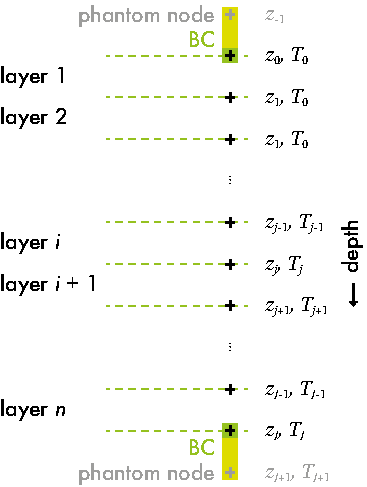
\includegraphics[]{numerical/figures/znodes.pdf}
    \caption{A one-dimensional discretization in space. Physical properties may
    be ascribed to the layers between each node (for one-dimension).  Phantom
    nodes may be placed outside the domain when flux boundary conditions are
    used.}
    \label{fig:znodes}
\end{figure}

Material properties may be associated either with the nodes themselves or with the intervals between nodes, depending on the formulation. For example, temperature is naturally defined at nodes, whereas properties such as thermal conductivity and heat production may be defined either at nodes or at the interfaces between them.

The choice of grid spacing $\Delta z$ is a modeling decision with direct physical consequences. Smaller values of $\Delta z$ reduce truncation error in finite difference approximations and allow sharper thermal gradients to be resolved. However, decreasing $\Delta z$ increases the number of nodes and therefore the computational cost of a solution.

In practice, grid spacing must balance accuracy against efficiency. A common approach is to repeat a calculation with progressively finer grids and verify that the solution converges within an acceptable tolerance. If halving $\Delta z$ produces negligible changes in the solution, the grid is sufficiently fine for the problem at hand.

Once the spatial domain has been discretized, the finite difference operators derived earlier are applied directly to the nodal values of temperature. For example, the second-order central difference approximation to the second derivative with respect to depth is written in discrete form as
\[
    \eval{\pdv[2]{T}{z}}_{z=z_j} \;\longrightarrow\;
    \frac{T_{j+1} - 2T_j + T_{j-1}}{\Delta z^2}.
\]

This operator measures the local curvature of the temperature field. If $T_j$ is larger than the average of its neighboring values, the curvature is negative and diffusion acts to reduce $T_j$. In this way, finite difference methods implement diffusion as a local balancing process repeated throughout the domain.

The pattern of nodes used to evaluate a finite difference operator is called a \emph{stencil}. For the second derivative in one dimension, the stencil consists of a central node and its immediate neighbors above and below (Figure~\ref{fig:fdstencils}). The stencil makes explicit that finite difference methods rely only on local information to approximate spatial derivatives.
\begin{figure}[htb]
    \centering
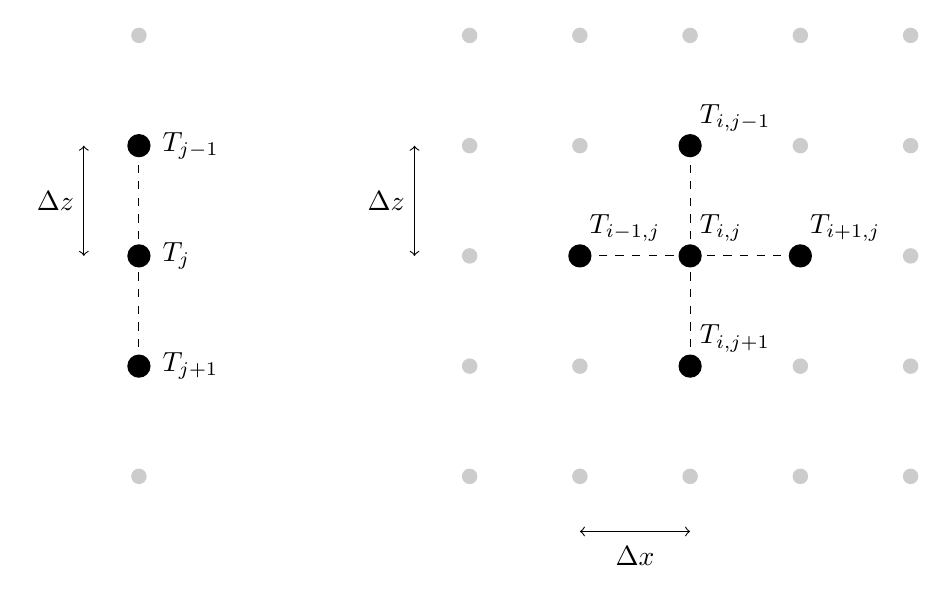
\begin{tikzpicture}[scale=1.4]
    \begin{scope}
        % Background grid nodes (faded)
        \foreach \k in {-2,2} {
            \fill[gray!40] (0,-\k) circle (2pt);
        }

        % Stencil nodes
        \fill (0,0) circle (3pt) node[right,xshift=5] {$T_{j}$};
        \fill (0,1) circle (3pt) node[right,xshift=5] {$T_{j-1}$};
        \fill (0,-1) circle (3pt) node[right,xshift=5] {$T_{j+1}$};

        % Dashed connections
        \draw[dashed] (0,0) -- (0,1);
        \draw[dashed] (0,0) -- (0,-1);

        % Delta z annotation
        \draw[<->] (-0.5,0) -- (-0.5,1) node[midway,left] {$\Delta z$};
    \end{scope}

    \begin{scope}[xshift=5cm]
        % Background grid (faded)
        \foreach \x in {-2,-1,0,1,2} {
            \foreach \z in {-2,-1,0,1,2} {
                \fill[gray!40] (\x,\z) circle (2pt);
            }
        }

        % Stencil nodes
        \fill (0,0) circle (3pt) node[right,yshift=10] {$T_{i,j}$};
        \fill (1,0) circle (3pt) node[right,yshift=10] {$T_{i+1,j}$};
        \fill (-1,0) circle (3pt) node[right,yshift=10] {$T_{i-1,j}$};
        \fill (0,1) circle (3pt) node[right,yshift=10] {$T_{i,j-1}$};
        \fill (0,-1) circle (3pt) node[right,yshift=10] {$T_{i,j+1}$};

        % Dashed stencil connections
        \draw[dashed] (0,0) -- (1,0);
        \draw[dashed] (0,0) -- (-1,0);
        \draw[dashed] (0,0) -- (0,1);
        \draw[dashed] (0,0) -- (0,-1);

        % Delta z annotation
        \draw[<->] (-2.5,0) -- (-2.5,1) node[midway,left] {$\Delta z$};
        \draw[<->] (-1,-2.5) -- (0,-2.5) node[midway,below,yshift=-2pt] {$\Delta x$};
    \end{scope}
\end{tikzpicture}
\caption{Stencils are the constructed connections between nodes used in finite difference approximations.  (a) One-dimensional finite difference stencil for the first and second derivative.  (b) Five-point stencil for the two-dimensional, first-derivative (gradient and divergence) or second-derivative (Laplacian).}
\label{fig:fdstencils}
\end{figure}

\subsection{Extension to two dimensions}

For problems involving lateral as well as vertical variations, the temperature field is written as $T(x,z,t)$. Discretizing both spatial directions leads to a two-dimensional grid with nodes indexed by $(i,j)$, where $i$ refers to the horizontal coordinate $x$ and $j$ to depth $z$.

Applying the same finite difference operators in each direction yields the standard five-point approximation to the Laplacian,
\[
    \eval{\pdv{T}{x}}_{x=x_i} + \eval{\pdv{T}{z}}_{z=zj} =  \;\longrightarrow\;
    \frac{T_{i+1,j} + T_{i-1,j} + T_{i,j+1} + T_{i,j-1} - 4T_{i,j}}{\Delta x^2},
\]
where $\Delta x = \Delta z$ is assumed for simplicity. This operator is the direct two-dimensional analogue of the one-dimensional second difference and follows from the same Taylor series arguments developed earlier.  The second difference measures the local \emph{curvature} of the temperature field. If $T_{i,j}$ is greater than the average of its neighbors, diffusion removes heat from that location. Finite differences therefore implement diffusion as a local balancing process.
The 2-D stencil in Figure~\ref{fig:fdstencils} can be used for either first- or second-order central differences.  

The discretization of space completes the transition from a continuous physical description of the Earth to a numerical representation suitable for computation. In the following sections we examine how boundary conditions are applied on this discrete grid and how time dependence is incorporated for transient problems.

\subsection{Steady-state problems: Poisson's equation}

The spatial discretization developed above can be used directly to solve
steady-state problems governed by elliptic equations. A common example in
geophysics is steady-state heat conduction with internal heat production,
described by Poisson's equation,
\[
    \pdv{}{z}\!\left(k \pdv{T}{z}\right) = -A,
\]
where $k$ is thermal conductivity and $A$ is volumetric heat production.

For constant thermal conductivity, this reduces to
\[
    \pdv[2]{T}{z} = -\frac{A}{k}.
\]
Using the second-order central difference derived earlier, the finite
difference approximation at node $z_j$ is
\[
    \frac{T_{j+1} - 2T_j + T_{j-1}}{\Delta z^2} = -\frac{A_j}{k}.
\]

Applying this equation at every interior node produces a system of linear
equations that can be written in matrix form,
\[
    \begin{bmatrix}
        1 & 0 & 0 & 0 & \cdots & 0 & 0 \\
        1 & -2 & 1 & 0 & \cdots & 0 & 0 \\
        0 & 1 & -2 & 1 & \cdots & 0 & 0 \\
        \vdots & \ddots & \ddots & \ddots & & \vdots & \vdots \\
        0 & \cdots & 0 & 1 & -2 & 1 & 0 \\
        0 & \cdots & 0 & 0 & 1 & -2 & 1 \\
        0 & 0 & 0 & 0 & 0 & 0 & 1
    \end{bmatrix}
    \begin{bmatrix}
        T_0 \\
        T_1 \\
        T_2 \\
        \vdots \\
        T_{J-2} \\
        T_{J-1} \\
        T_J
    \end{bmatrix}
    =
    \begin{bmatrix}
        T_0^{\text{bc}} \\
        -\dfrac{A_1 \Delta z^2}{k} \\
        -\dfrac{A_2 \Delta z^2}{k} \\
        \vdots \\
        -\dfrac{A_{J-2} \Delta z^2}{k} \\
        -\dfrac{A_{J-1} \Delta z^2}{k} \\
        T_J^{\text{bc}}
    \end{bmatrix}.
\]
Boundary conditions supply the additional equations needed to close the system. Solving this system yields the steady-state temperature profile directly, without time stepping.  This system is tridiagonal, reflecting the local nature of the finite difference stencil. If thermal conductivity varies with depth, the coefficients in the matrix change, but the tridiagonal structure of the system is preserved.

\subsection{Boundary Conditions}

Just as boundary conditions are required to obtain analytic solutions to partial differential equations, they are also essential for numerical solutions. In finite difference methods, boundary conditions provide the additional information needed to evaluate derivatives at the edges of a discretized domain and therefore play a central role in determining the
behavior of the solution.

Unlike interior points, where symmetric finite difference operators can be applied, boundary nodes lack information on one side. As a result, the choice and implementation of boundary conditions directly affect numerical accuracy and stability. In many practical problems, numerical errors are dominated not by the discretization of the interior, but by the treatment of boundaries.

\subsubsection{Boundary Condition Types}

Boundary conditions encountered in geophysical modeling are commonly grouped into three main types (Table~\ref{tab:bc}). A fourth category, sometimes referred to as a Cauchy condition, arises when different boundary types are applied on different parts of the domain.
\begin{table}[htbp]
    \centering
    \caption{Types of boundary conditions for discrete PDE methods.}
    \label{tab:bc}
    \begin{tabularx}{0.75\textwidth}{llX}
    \toprule
    Type & Mathematical form & Geophysical meaning \\
    \midrule
    Dirichlet (fixed) & $T = T_0$ & Fixed temperature (e.g., surface or magma temperature) \\
    Neumann (fixed flux) & $\displaystyle \pdv{T}{z} = \frac{q}{k}$ & Prescribed heat flux (e.g., basal heat flow) \\
    Neumann (zero flux) & $\displaystyle \pdv{T}{z} = 0$ & No heat flow across boundary (reflecting) \\
    Robin (mixed) & $aT + b\pdv{T}{z} = c$ & Coupled boundary (e.g., atmosphere--ground exchange) \\
    \bottomrule
    \end{tabularx}
\end{table}

A \emph{Dirichlet}, or fixed, boundary condition specifies the value of the field at the boundary and is straightforward to implement numerically.

A \emph{Neumann}, or fixed-flux, boundary condition specifies the gradient of the field at the boundary and therefore constrains the flow of heat rather than the temperature itself. A special case of the Neumann condition is the zero-flux boundary, which enforces no heat transfer across the boundary.

\emph{Robin} boundary conditions represent a linear combination of value and flux at the same boundary and commonly arise when the boundary interacts with an external reservoir, such as heat exchange between the ground and the atmosphere.

\emph{Cauchy} boundary conditions, in the strict mathematical sense, refer to situations where different boundary types are applied on different parts of the domain. In practice, most geophysical applications can be described using Dirichlet, Neumann, or Robin conditions.

In a finite difference model, boundary conditions must be enforced at specific
nodes. For Dirichlet conditions, this is accomplished by directly assigning
the boundary value to the appropriate node.

\subsection{Flux Conditions at Boundaries}

Neumann and Robin conditions require additional care because they involve derivatives at the boundary. Evaluating a derivative at a boundary node requires information beyond the edge of the computational domain. To handle this, it is common to introduce a \emph{phantom node} outside the domain.

For example, consider a Neumann boundary condition imposed at the surface,
\[
    \left.\pdv{T}{z}\right|_{z=z_0} = g.
\]
Using a finite difference approximation, this derivative can be written as
\[
    \frac{T(z_1) - T(z_{-1})}{2\Delta z} = g,
\]
where $T(z_{-1})$ is a phantom node located outside the domain. This relation allows the phantom-node value to be expressed in terms of interior nodes and the prescribed flux, ensuring that the boundary condition is satisfied while maintaining second-order accuracy.

Boundary conditions do more than close a mathematical system; they encode physical assumptions about how the modeled region interacts with its surroundings. This is especially important in geophysical problems dominated by vertical heat flow.

A fixed-flux boundary condition allows heat to enter or leave the domain at a specified rate. For example, prescribing basal heat flow permits heat to continuously enter the lithosphere from below. In contrast, a zero-flux boundary condition is reflecting: it prevents heat from crossing the boundary entirely. Any heat that would otherwise leave the system is instead reflected back into the domain.

When applied to vertical boundaries in models dominated by vertical heat transport, zero-flux conditions can strongly influence the solution. They effectively assume that no lateral heat exchange occurs across the boundary, which may or may not be physically appropriate depending on the scale of the model and the geological setting. As a result, zero-flux boundaries should be used deliberately and interpreted carefully.

\subsection{Why boundary conditions dominate solutions}

Because elliptic and parabolic equations communicate information throughout the domain, boundary conditions exert a global influence on the solution. An incorrect or poorly implemented boundary condition can overwhelm the effects of interior discretization, leading to solutions that are numerically stable but physically misleading.

For this reason, boundary conditions should be viewed not as technical details, but as integral components of the physical model. In geophysical applications, they encode assumptions about surface processes, basal heat input, and the degree to which the modeled system is isolated or interacting with its surroundings.

\subsection{Sharp property gradients}

Many geologic systems contain sharp spatial variations in material properties.  Examples include layered sediments, faults, lithologic contacts, and the transition from crust to mantle. In such cases, thermal conductivity, heat capacity, or diffusivity may change abruptly over distances comparable to or smaller than the grid spacing.

Sharp property gradients present a challenge for finite difference methods because standard central difference operators implicitly assume that coefficients vary smoothly across a stencil. When this assumption is violated, naïve discretizations can produce unphysical temperature profiles or incorrect heat fluxes.

For heat conduction, the physically relevant quantity is not temperature itself, but heat flux. At a material interface, temperature may have a kink (change in gradient), but heat flux must remain continuous. In one dimension, this requires
\[
    k_1 \eval{\pdv{T}{z}}_{\text{above}} = k_2 \eval{\pdv{T}{z}}_{\text{below}} .
\]

Finite difference schemes must therefore be constructed to preserve flux continuity across interfaces. Harmonic averaging and grid refinement are two methods that can be employed at abrupt boundaries.

A common and effective approach is to define thermal conductivity at the interfaces between nodes rather than at the nodes themselves. For two adjacent nodes with conductivities $k_i$ and $k_{i+1}$, the interface conductivity is often taken as the harmonic mean,
\[
    k_{i+1/2} = \left( \frac{1}{2}\left[\frac{1}{k_i} + \frac{1}{k_{i+1}}\right] \right)^{-1}.
\]
Using interface conductivities ensures that heat flux is treated consistently across sharp contrasts and avoids artificial thermal barriers or sinks.

Another strategy is to increase spatial resolution (grid refinement) near sharp property contrasts. Refining the grid allows abrupt changes to be better resolved and reduces truncation error. However, refinement increases computational cost and may impose stricter timestep constraints for explicit schemes.

When sharp gradients coincide with material boundaries, it is often preferable to align grid nodes with those interfaces. In this case, properties are piecewise constant within layers, and interfaces fall exactly between nodes.  This approach simplifies implementation and improves physical interpretation, especially in layered media.

Strongly heterogeneous materials, thin layers, or irregular interfaces can push finite difference methods beyond their natural strengths. In such cases, finite volume methods (which enforce flux conservation explicitly) or finite element methods (which accommodate complex geometries) may be better suited.

Nevertheless, with careful treatment of fluxes, grid design, and averaging, finite difference methods can successfully model many problems involving sharp property gradients.


\section{Discretizing Time}

Now that we've covered the spatial differences, we need to develop a formulation for those fields which vary in time as well as space (i.e., transient, not steady-state).  As with space, time is treated as a continuous variable that is replaced by a discrete representation. The solution is evaluated at a sequence of time levels separated by a timestep $\Delta t$, and finite difference approximations are used to estimate time derivatives. The combined discretization of space and time converts time-dependent partial differential equations into iterative rules that advance the solution from one time level to the next.

Mirroring the spatial discritization methods that we developed earlier, there are three primary ways that we can formulate temporal differences:
\begin{itemize}
    \item A forward difference, \emph{explicit method}, is the cheapest to compute numerically, but can suffer from stability issues if the discretization is not designed properly.  An explicit formulation is relatively straightforward because it seeks to predict the future based on the present. 
    \item  A backwards difference, \emph{implicit method}, is a bit awkward because you are attempting to determine the past based on the future (although we really are solving for the future).  While more costly to solve, the advantage of an implicit formulation is numerical stability.
    \item A central difference, \emph{Crank-Nicholson method}, averages the implicit and explicit methods for numerical stability and improved accuracy.
\end{itemize}

\subsection{Discretization in space and time}

To examine discritization in space and time, we'll examine the diffusion equation in one dimensions,
\[
    \pdv{T}{t} = kappa  \pdv[2]{T}{z} .
\]
Consider a one-dimensional vertical domain discretized in space with nodes at depths $z_j$, as before. Time is discretized into levels $t^n$, where $n$ indexes the timestep (Figure~\ref{fig:ztnodes}). The temperature at depth $z_j$ and time $t^n$ is denoted $T_j^n$.
\begin{figure}[bthp]
    \centering
    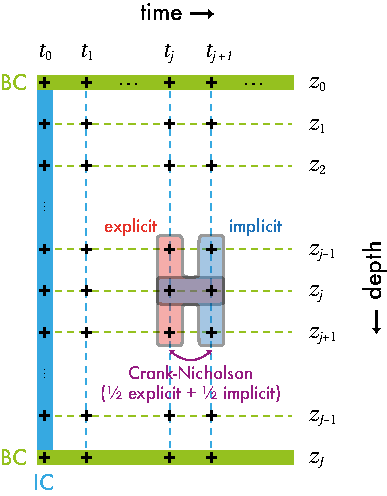
\includegraphics[]{numerical/figures/ztnodes.pdf}
    \caption{A discretization in space and time. Solving a PDE dependent on time and can be done either solving for the future (explicit), 'solving' for the past (implicit), or a mix of both (Crank-Nicholson).}
    \label{fig:ztnodes}
\end{figure}

Finite difference approximations in time mirror those used in space. A forward difference in time estimates the time derivative using information from the present state, while a backward difference estimates it using information from the future state. As in space, the choice of approximation has important implications for accuracy and stability.

\subsection{Physical meaning of time stepping}

Time stepping controls the rate at which information can propagate through the numerical model. For diffusive processes such as heat transport, information propagates through local interactions between neighboring nodes. In a single timestep, changes at a node can influence only adjacent nodes.

If the timestep is chosen too large, the numerical scheme attempts to transmit information faster than the underlying physics allows. In effect, the model is asked to move heat farther in one timestep than diffusion permits---it's like exceeding the speed of light...it can't be done. When this happens, the solution becomes unstable and nonphysical.

This limitation is not merely numerical; it reflects the physics of diffusion.  Numerical schemes must respect the finite rate at which diffusive processes redistribute heat.

\subsection{Explicit (forward-in-time) method}

Consider the one-dimensional heat diffusion equation with constant properties,
\[
    \pdv{T}{t} = \kappa \pdv[2]{T}{z}.
\]
Since many geologists and geochemists encounter diffusion outside of geophysics, it is worth noting that chemical diffusion follows an identical mathematical form. Replacing temperature $T$ with concentration $C$ and thermal diffusivity $\kappa$ with chemical diffusivity $D$ yields the corresponding equation for chemical transport.

Using a forward difference in time and a second-order central difference in space, the finite difference approximation at depth $z_j$ and time $t^{n+1}$ is
\[
    \workeq
    \frac{T_j^{n+1} - T_j^n}{\Delta t} =
    \kappa \frac{T_{j+1}^n - 2T_j^n + T_{j-1}^n}{\Delta z^2}.
\]
Solving for the future temperature gives
\[
    \workeq
    T_j^{n+1} = T_j^n +
    \kappa \frac{\Delta t}{\Delta z^2} \left(T_{j+1}^n - 2T_j^n + T_{j-1}^n\right).
\]

This explicit scheme predicts the future state entirely from the present. It is computationally efficient and straightforward to implement, but it is only stable if the timestep is sufficiently small. Because information propagates only between neighboring nodes in a single timestep, the timestep must satisfy the stability condition
\[
    \coreeq
    \kappa \frac{\Delta t}{\Delta z^2} \le \frac{1}{2}.
\]
If this inequality is violated, numerical errors grow rapidly and the solution becomes unstable. Higher-order spatial discretizations alter the stability criterion but do not remove the fundamental restriction on timestep size.

\subsection{Implicit (backward-in-time) method}

An alternative approach is to evaluate spatial derivatives at the future time level. Using a backward difference in time gives
\[
    \workeq
    \frac{T_j^{n+1} - T_j^n}{\Delta t} =
    \kappa \frac{T_{j+1}^{n+1} - 2T_j^{n+1} + T_{j-1}^{n+1}}{\Delta z^2}.
\]

Rearranging terms places all unknown future temperatures on one side,
\[
    \workeq
    -\kappa \frac{\Delta t}{\Delta z^2} T_{j-1}^{n+1} +
    \left(1 + 2\kappa \frac{\Delta t}{\Delta z^2}\right) T_j^{n+1} -
    \kappa \frac{\Delta t}{\Delta z^2} T_{j+1}^{n+1} =
    T_j^n .
\]

For a domain with fixed temperatures at its boundaries (Dirichlet boundary conditions), the full system of equations can be written explicitly as
\begin{align*}
    T_0^{n+1} &= T_0^{n}, \\
    -\alpha T_{0}^{n+1} + (1 + 2\alpha) T_1^{n+1} - \alpha T_{2}^{n+1} &= T_1^n, \\
    -\alpha T_{1}^{n+1} + (1 + 2\alpha) T_2^{n+1} - \alpha T_{3}^{n+1} &= T_2^n, \\
    &\vdots \\
    -\alpha T_{J-2}^{n+1} + (1 + 2\alpha) T_{J-1}^{n+1} - \alpha T_{J}^{n+1} &= T_{J-1}^n, \\
    T_J^{n+1} &= T_J^{n},
\end{align*}
where $\alpha = \kappa \Delta t / \Delta z^2$.  While this looks like we are using the future to solve for the past, we really don't know the future temperatures and need to solve for it by solving this system of equations.  Because this is a system of linear equations it is easy to write the above result in matrix form:
\begin{align*}
    \begin{bmatrix}
        1 & 0 & 0 & 0 & \cdots & 0 & 0 & 0 & 0 \\
        -\alpha & (1 + 2\alpha) & -\alpha & 0 & \cdots & 0 & 0 & 0 & 0 \\
        0 & -\alpha & (1 + 2\alpha) & -\alpha & \cdots & 0 & 0 & 0 & 0 \\
        \vdots & \ddots & \ddots & \ddots & & & & \vdots \\
        0 & 0 & 0 & 0 & \cdots & -\alpha & (1 + 2\alpha) & -\alpha & 0 \\
        0 & 0 & 0 & 0 & \cdots & 0 & -\alpha & (1 + 2\alpha) & -\alpha \\
        0 & 0 & 0 & 0 & \cdots & 0 & 0 & 0 & 1
    \end{bmatrix}
    \begin{bmatrix}
        T_{0}^{n+1} \\
        T_{1}^{n+1} \\
        T_{2}^{n+1} \\
        \vdots \\
        T_{J-2}^{n+1} \\
        T_{J-1}^{n+1} \\
        T_{J}^{n+1}
    \end{bmatrix}
    = \begin{bmatrix}
        T_{0}^n \\
        T_{1}^n \\
        T_{2}^n \\
        \vdots \\
        T_{J-2}^n \\
        T_{J-1}^n \\
        T_{J}^n
    \end{bmatrix}.
\end{align*}
Note that the matrix is sparse except for values along the diagonal and just above and below.  This is called a tridiagonal matrix.  This system can be written compactly in matrix form as
\[
    \mathbf{A}\,\mathbf{T}^{n+1} = \mathbf{T}^n,
\]
where $\mathbf{A}$ is a tridiagonal matrix. Although it is possible to invert $\mathbf{A}$ directly, this is computationally inefficient. Instead, numerical methods exploit the tridiagonal structure to solve the system rapidly and with minimal memory usage.

The implicit method is unconditionally stable: it remains stable for any choice of $\Delta t$. The cost of this stability is the need to solve a system of equations at each timestep.

\subsection{Crank--Nicolson method}

The Crank--Nicolson method combines the explicit and implicit approaches by averaging the spatial derivative between the current and future time levels,
\[
    \workeq
    \frac{T_j^{n+1} - T_j^n}{\Delta t} = \frac{\kappa}{2}
    \left[
    \frac{T_{j+1}^{n+1} - 2T_j^{n+1} + T_{j-1}^{n+1}}{\Delta z^2} +
    \frac{T_{j+1}^{n} - 2T_j^{n} + T_{j-1}^{n}}{\Delta z^2}
    \right].
\]
As with the implicit scheme, this formulation leads to a tridiagonal system of equations that can be solved efficiently.
Separating the future timestep from the current timestep,
\begin{equation*}
    \workeq
    -\beta T_{j+1}^{n+1} + (1 + 2\beta) T_j^{n+1} - \beta T_{j-1}^{n+1} =
    \beta T_{j+1}^{n} + (1 - 2\beta) T_j^{n} + \beta T_{j-1}^{n} ,
\end{equation*}
where $\beta = \frac{1}{2} \kappa \Delta t \Delta z^{-2}$.  Again we can write this in matrix form producing a tridiagonal matrix,
\begin{align*}
    \resizebox{\textwidth}{!}{$
    \begin{bmatrix}
        1 & 0 & 0 & 0 & \cdots & 0 & 0 & 0 & 0 \\
        -\beta & (1 + 2\beta) & -\beta & 0 & \cdots & 0 & 0 & 0 & 0 \\
        0 & -\beta & (1 + 2\beta) & -\beta & \cdots & 0 & 0 & 0 & 0 \\
        \vdots & \ddots & \ddots & \ddots & & & & \vdots \\
        0 & 0 & 0 & 0 & \cdots & -\beta & (1 + 2\beta) & -\beta & 0 \\
        0 & 0 & 0 & 0 & \cdots & 0 & -\beta & (1 + 2\beta) & -\beta \\
        0 & 0 & 0 & 0 & \cdots & 0 & 0 & 0 & 1
    \end{bmatrix}
    \begin{bmatrix}
        T_{0}^{n+1} \\
        T_{1}^{n+1} \\
        T_{2}^{n+1} \\
        \vdots \\
        T_{J-2}^{n+1} \\
        T_{J-1}^{n+1} \\
        T_{J}^{n+1}
    \end{bmatrix}
    = 
    \begin{bmatrix}
        T_0^n \\
        \beta T_0 + (1 + 2\beta) T_1^n + \beta T_2^n \\
        \beta T_1^n + (1 + 2\beta) T_2^n + \beta T_3^n \\
        \vdots \\
        \beta T_{J-3}^n + (1 + 2\beta) T_{J-2}^n + \beta T_{J-1}^n \\
        \beta T_{J-2}^n + (1 + 2\beta) T_{J-1}^n + \beta T_{J}^n \\
        T_{J}^n
    \end{bmatrix} .
    $}
\end{align*}

The Crank--Nicolson method is second-order accurate in time and stable for linear diffusion problems, providing a balance between numerical accuracy and stability.

\subsection{Depth-dependent sources}

Many geophysical systems include internal sources that vary with depth, such as
radiogenic heat production concentrated in the crust. These sources can be
incorporated naturally into transient diffusion problems.

Including a depth-dependent heat production term $A(z)$, the heat diffusion
equation becomes
\[
    \pdv{T}{t} = \kappa \pdv[2]{T}{z} + \frac{A(z)}{\rho C_P}.
\]
Using a Crank--Nicolson formulation, the finite difference approximation at node $z_j$ is
\[
    \frac{T_j^{n+1} - T_j^n}{\Delta t} =
    \frac{\kappa}{2} \left[
    \frac{T_{j+1}^{n+1} - 2T_j^{n+1} + T_{j-1}^{n+1}}{\Delta z^2} +
    \frac{T_{j+1}^{n} - 2T_j^{n} + T_{j-1}^{n}}{\Delta z^2}
    \right] + \frac{A_j}{\rho C_P} .
\]

The source term appears as an additional contribution to the right-hand side of the system. Importantly, it does not change the coupling between nodes. The resulting system of equations remains tridiagonal and can be solved using the same numerical techniques as in the source-free case.  Depth-dependent sources therefore increase physical realism without altering
the fundamental numerical structure of the problem.

\subsection{Initial conditions}

Time-dependent problems require not only boundary conditions in space, but also an initial condition in time. While boundary conditions constrain how the system interacts with its surroundings, the initial condition specifies the
state of the system at the starting time.  For thermal diffusion problems, the initial condition prescribes the temperature field at time $t = 0$,
\[
    T(z,0) = T_0(z),
\]
or, in discretized form,
\[
    T_j^{0} = T_0(z_j).
\]

The initial condition provides the starting values from which the solution is advanced forward in time. In explicit schemes, these values are used directly to compute the temperature at the next timestep. In implicit and Crank--Nicolson schemes, the initial condition forms the right-hand side of the first system of equations to be solved.  

Initial conditions are not merely mathematical conveniences; they encode physical assumptions about the prior thermal state of the system. Examples include a steady-state geotherm, a uniform initial temperature, or a temperature profile inherited from an earlier tectonic or thermal event.  As with boundary conditions, inappropriate or inconsistent initial conditions can dominate the solution, especially at early times. Careful choice of initial conditions is therefore essential for meaningful transient modeling.

\subsection{Summary of temporal schemes}

Explicit, implicit, and Crank--Nicolson methods differ primarily in how they handle directionality in time. Explicit schemes are forward-looking and computationally inexpensive, but limited by stability constraints. Implicit schemes are backward-looking and stable for any timestep, but require the solution of a linear system. Crank--Nicolson schemes are symmetric in time and offer improved accuracy at the cost of increased computational effort.

As with spatial discretization and boundary conditions, the choice of time stepping scheme reflects a balance between physical realism, numerical stability, and computational efficiency.

\section{PDE Classes}

The numerical behavior of a finite difference model depends strongly on the class of partial differential equation being solved. Although the same basic difference operators appear in many problems, elliptic, parabolic, and hyperbolic equations differ fundamentally in how information propagates through the domain and how solutions must be computed.

The table below summarizes these distinctions using temperature as a unifying example.
\begin{table}
    \centering
    \caption{Common geophysical field equations and their numerical methods.}
    \label{tab:fdpde}
    \begin{tabular}{lcll}
        \toprule
        PDE type & Equation & Information behavior & Numerical consequence \\
        \midrule
        elliptic & $\nabla^2 T = s$ & instantaneous & global solve \\
        parabolic & $\pdv{T}{t} = \kappa\nabla^2T$ & spreads gradually & timestep tied to diffusioin \\
        hyperbolic & $\pdv{T}{t} = c^2\nabla^2T$ & travels at fixed speed & timestep tied to wave speed \\
        \bottomrule
    \end{tabular}
\end{table}

Elliptic equations describe systems in steady state, where changes at one location influence the entire domain instantaneously. Finite difference solutions therefore require solving a global system of equations.

Parabolic equations describe diffusive processes, where information propagates gradually and the system evolves in time. Finite difference solutions advance incrementally, and numerical stability depends on the timestep.

Hyperbolic equations describe wave-like behavior, where information propagates along characteristic paths at finite speed.
The timestep for these problems is limited by how fast information can move through the grid. If the numerical scheme allows a wave to travel farther than one grid cell in a single timestep, the model becomes unstable. In effect, the code is trying to move information faster than the physics allows, and it fails spectacularly.

Finite difference schemes for such equations are constrained by causality and require careful treatment of time stepping and boundary conditions.

\section{Verification}

Numerical solutions should not be accepted on faith. Whenever possible, finite difference models should be tested against analytic solutions or well-known limiting cases. This process, known as verification, ensures that the numerical implementation correctly solves the governing equations.

Common analytic benchmarks for thermal problems include:
\begin{itemize}
  \item steady-state geotherms in homogeneous slabs with prescribed boundary
  temperatures or heat fluxes;
  \item plate cooling or heating of a half-space following a step change
  in boundary temperature.
\end{itemize}

Agreement with analytic solutions builds confidence in the numerical method.  Disagreement usually indicates problems with boundary conditions, grid resolution, timestep choice, or indexing rather than with the physics itself.

Verification should be viewed as an essential part of model development rather than an optional check.

\section{Beyond Linearity}

Most examples in this chapter have assumed constant material properties, planar boundaries, and linear governing equations. These assumptions are useful for developing intuition, but real geologic systems are rarely so simple.  Finite difference methods are flexible enough to accommodate many departures from linearity, provided they are introduced carefully.

Many geophysical problems include sources or sinks that add or remove heat within the domain. Examples include radiogenic heat production, latent heat associated with phase changes, or chemical reactions.  For transient heat diffusion, an internal source term $A(z)$ can be included directly in the governing equation,
\[
    \pdv{T}{t} = \kappa \pdv[2]{T}{z} + \frac{A}{\rho c_p}.
\]
In a finite difference formulation, source terms enter as additional terms in the update equation at each node. Conceptually, they act as local forcing that raises or lowers temperature independent of diffusion.

In many geologic settings, thermal conductivity is directionally dependent.  Layered sediments, foliated metamorphic rocks, and fractured media may conduct heat more efficiently in one direction than another.  Anisotropy is handled naturally in finite difference methods by allowing different conductivities (or diffusivities) in different coordinate directions. In two dimensions, this leads to diffusion terms of the form
\[
\pdv{}{x}\!\left(k_x \pdv{T}{x}\right)
+
\pdv{}{z}\!\left(k_z \pdv{T}{z}\right),
\]
which can be discretized using the same stencil ideas developed earlier, with direction-dependent coefficients.

Thermal conductivity, heat capacity, and diffusivity often vary with temperature. Pressure dependence is commonly incorporated by prescribing depth- dependent properties at the outset of a model, but temperature dependence introduces true nonlinearity.  In finite difference models, temperature-dependent properties are typically handled iteratively. At each timestep, material properties are updated using the current temperature field, and the governing equations are solved again using the updated values. Convergence is assessed by monitoring changes in the solution between iterations.

\subsection{Topography and nonplanar boundaries}

The Earth's surface and many internal boundaries are not flat. Surface topography and basal relief can strongly influence heat flow, especially near the surface.

In finite difference methods, nonplanar boundaries are often handled by:
\begin{itemize}
  \item mapping the physical domain onto a rectangular computational grid;
  \item approximating topography using stair-step boundaries aligned with the grid;
  \item or modifying boundary conditions locally to account for variable surface elevation.
\end{itemize}

While such approaches can be effective, strongly irregular geometries often motivate the use of finite element or finite volume methods, which handle complex boundaries more naturally.

\section{Other Methods}

Finite difference methods are among the simplest and most transparent ways to solve partial differential equations, but they also have important limitations:
\begin{itemize}
    \item Finite difference methods are most naturally formulated on structured (logically rectangular) grids, which can make complex geometries and highly irregular boundaries difficult to represent accurately.
    \item Grid refinement around regions of interest is possible, but often leads to large aspect ratios or strongly varying cell sizes elsewhere in the domain, which can degrade numerical accuracy or impose restrictive timestep constraints.
    \item When material advects through the domain, finite difference models must either track properties moving through a fixed grid or deform the grid itself. Grid deformation can introduce very small cell sizes that require correspondingly small timesteps to maintain stability.
\end{itemize}

Finite differences are therefore not the only option. Two other approaches are widely used in geophysics and engineering: finite element methods and finite volume methods.

Finite element methods (FEM) approximate the solution using basis functions defined over elements that tile the domain. They are particularly well suited to complex geometries, irregular boundaries, and strongly heterogeneous materials.  Finite element meshes can be refined locally around regions of interest and can be deformed more naturally to accommodate material motion and advection.  Compared to finite difference methods, FEM formulations are mathematically and computationally more complex, but offer greater geometric flexibility.

Finite volume methods (FVM) enforce conservation laws by integrating governing equations over control volumes. Fluxes are computed explicitly across volume boundaries, making these methods especially effective for problems where strict conservation is critical, such as fluid flow, mass transport, and reactive systems. In some formulations, control volumes can move with the material, providing a natural framework for advection while preserving conservation.

Compared to finite differences:
\begin{itemize}
  \item finite difference methods are conceptually simpler and easier to implement;
  \item finite element methods handle complex geometries and boundary conditions more naturally;
  \item finite volume methods emphasize conservation and robustness, particularly in advective systems.
\end{itemize}

\section{Looking Ahead}

In this course, we have focused on finite difference methods because they provide a direct and transparent connection between physical laws and their numerical implementation. This clarity makes finite differences especially well suited for developing intuition about how geophysical systems behave and how numerical models encode physical assumptions. Finite element and finite volume methods are typically introduced in more advanced numerical modeling courses, where their additional mathematical and computational complexity can be addressed in greater depth.

The techniques developed in this chapter form the foundation for modeling many realistic geophysical systems. Incorporating nonlinearity, anisotropy, sharp property contrasts, and complex boundaries increases physical realism, but also demands greater care in assessing stability, convergence, and physical interpretation. These challenges motivate more sophisticated discretization strategies and solution methods, some of which were briefly introduced here and are treated more fully in advanced courses.

Numerical forward models such as those developed in this chapter are also a central component of inversion theory. Inverse problems seek to infer subsurface properties or boundary conditions from observations by repeatedly evaluating forward models and comparing their predictions to data. The accuracy, stability, and efficiency of finite difference solutions therefore play a key role in determining what information can be reliably extracted from geophysical measurements. The next chapter builds on the numerical foundations developed here to introduce the principles of inversion and data interpretation.

\chapter[Inversion Theory: Foundations]{Inversion Theory\\ {\LARGE Foundations}}\label{ch:inversion}

\epigraph{``Reports that say that something hasn't happened are always interesting to me, because as we know, there are known knowns; there are things we know we know. We also know there are known unknowns; that is to say we know there are some things we do not know. But there are also unknown unknowns---the ones we don't know we don't know. And if one looks throughout the history of our country and other free countries, it is the latter category that tend to be the difficult ones.''}
{{\normalfont ---\ Donald Rumsfeld}}

\section{Introduction}
This quote is often treated humorously, but it captures a fundamental relationship between knowledge and information that lies at the heart of scientific inference. In geophysics, and particularly in inversion theory, we are constantly navigating between what we believe we understand about the Earth and what remains uncertain, hidden, or even unsuspected. Figure~\ref{fig:rumsfeld} provides a conceptual framework for organizing these ideas.

\begin{figure}[hbtp]
    \centering
    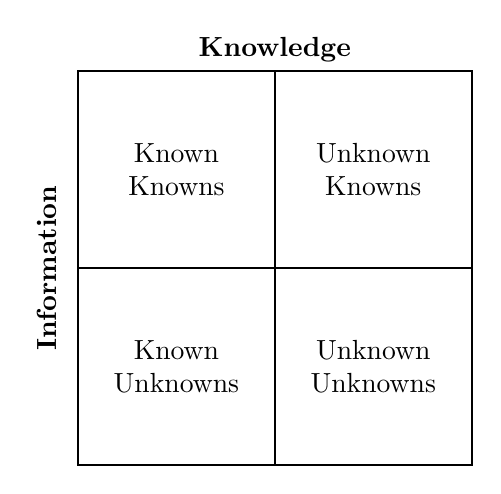
\begin{tikzpicture}[scale=1, every node/.style={align=center}]
        % Axes
        \draw[-, thick] (-2.5,0) -- (2.5,0);
        \node[rotate=90] at (-2.9, 0) {\textbf{Information}};
        \draw[-, thick] (0,-2.5) -- (0,2.5);
        \node[above] at (0, 2.5) {\textbf{Knowledge}};

        % Quadrants
        \draw[thick] (-2.5,-2.5) rectangle (2.5,2.5);

        % Labels
        \node at (-1.25,1.25) {Known\\ Knowns};
        \node at (-1.25,-1.25) {Known\\ Unknowns};
        \node at (1.25,1.25){Unknown\\ Knowns};
        \node at (1.25,-1.25){Unknown\\ Unknowns};

    \end{tikzpicture}
    \caption{Conceptual diagram, now called the Rumsfeld Matrix, can be used to describing the relationship between knowledge of a system and its properties.}
    \label{fig:rumsfeld}
\end{figure}


In its simplest form, \emph{inversion} is the process of using observations to infer properties of a system. More precisely, inversion seeks to estimate unknown properties of a system using measurements and a set of assumed physical laws**. Because observations are always incomplete and noisy, inversion is not merely a process of calculation, but one of reasoning: validating what is known, quantifying what is uncertain, and recognizing the limits of inference.

The four quadrants of Figure~\ref{fig:rumsfeld} highlight different relationships between information and knowledge:
\begin{description}
    \item[Known Knowns:]
    Characteristics of a system that we are aware of and explicitly represent. These include established physical laws, known geological processes, mapped structures, and assumptions that are consciously incorporated into models and forward operators.

    \item[Known Unknowns:]
    Aspects of the system that we recognize as uncertain. These are quantities we know exist but do not know their values, such as subsurface property distributions or interface geometries. Inversion methods are designed primarily to estimate these quantities.

    \item[Unknown Knowns:]
    Information about the system that we possess but do not yet recognize as knowledge. This information may be encoded implicitly in data structure, correlations, contextual understanding, or prior experience, but is not explicitly incorporated into the model. Much scientific progress involves recognizing and formalizing such information.

    \item[Unknown Unknowns:]
    Aspects of the system that lie outside our awareness and violate our assumptions. These include missing or incorrect physics, unrecognized processes, or fundamentally invalid model hypotheses. Persistent or systematic misfit between observations and predictions may signal the presence of unknown unknowns.
\end{description}

In this sense, inversion is not solely about estimating parameters. Progress often comes from recognizing structure in residuals, realizing constraints we already had, and promoting information from unknown knowns to known knowns or unknown unknowns to known unknowns.

Inversion theory has deep roots in geophysics. Unlike many laboratory sciences, where experiments are designed to isolate unknown physical processes, geophysics more often applies well-established physics to systems whose source distributions or material properties are unknown. We measure fields at or near the Earth's surface and seek to infer the properties and structures that produced them. This reversal---known physics applied to unknown causes---is precisely the setting in which inverse problems arise.

To illustrate the distinction between forward and inverse problems, consider the simple linear relationship
\[
    y = mx .
\]
If the values of $m$ and $x$ are known, this equation can be used to predict $y$; this is a forward problem. In reality, $y$ is measured at the conditions of $x$, but the property of the system, $m$, is unknown.  The equation can be rearranged, inverted, to solve for $m$,
\[
    m = \frac{y}{x} .
\]
This is a trivial example of an inverse problem: determining an unknown quantity from observations using a known relationship.

Most geophysical inverse problems are far more complicated. The relationships between observations and properties are often nonlinear, the number of unknowns may exceed the number of measurements, and observations are contaminated by noise. In such cases, inversion is no longer a matter of algebraic rearrangement, but requires systematic approaches to estimation, uncertainty, and interpretation. The remainder of this chapter develops the framework needed to address these challenges.

\section{Notation}

\begin{table}[h!]
    \centering
    \begin{threeparttable}
    \caption{Notation used for inverse theory in this text.}
    \label{tab:inverse_notation}
    \begin{tabularx}{0.65\textwidth}{@{}cX@{}}
        \toprule
        \textbf{Symbol} & \textbf{Quantity} \\
        \midrule
        $\vb{d}, (\vb{\tilde{d}})$    & data (pseudodata) vector \\
        $\vb{m}$    & model vector \\
        $\Fop$      & forward model/operator \\
        $\vb{J}$    & linearized sensitivity/Jacobian \\
        $\vb{A}$    & linear forward matrix\tnote{a} \\
        $\vb{C}$    & covariance \\
        $\phi$      & objective/misfit function \\
        $\vb{L}$    & regularization operator \\
        $\vb{r}$    & residual \\
        $\vb{W}$    & weighting matrix \\
        $\epsilon$  & noise/error \\
        $\lambda$   & Lagrangian multiplier/regularization hyperparmeter\tnote{b} \\
        $\Delta$    & small perturbation (step) \\
        \bottomrule
    \end{tabularx}
    \begin{tablenotes}
    \item[a] While we use $\vb{A}$ in this text, $\vb{G}$ is probably more common in geophysics.  We use $\vb{A}$ so it is not confused with the gravitational constant.
    \item[b] Hyperparameters are external (non-physical) variables that are used to tune a the behavior/performance of the inversion.  These are either set manually by the user or optimized by a grid search or some other process. They affect the complexity and accuracy of an inversion.
    \end{tablenotes}
    \end{threeparttable}
\end{table}


\section{Inversion and Curve-Fitting}

At its core, inversion is a problem of estimation. Observations are related to a set of parameters through a mathematical model, and the objective of inversion is to determine the parameter values that best explain the data. In this sense, geophysical inversion is not fundamentally different from curve fitting or regression: both seek to infer unknown quantities from measurements using an assumed functional relationship.

This perspective is useful because it emphasizes that inversion methods are not uniquely tied to geophysics. The same mathematical framework can be applied to a wide variety of problems, including fitting experimental data in the laboratory, calibrating analytic models, analyzing synthetic data, or interpreting field observations. What distinguishes geophysical inversion is not the mathematics itself, but the physical meaning ascribed to the parameters and the interpretation of the resulting models.

Historically, inversion techniques have emerged independently in multiple disciplines, often under different names and with different terminology (Box~\ref{box:inverse_terms}). In statistics, similar problems are referred to as estimation or regression; in data science and machine learning, they are described in terms of training models or fitting predictors. Despite these differences in language, the underlying ideas are closely related. Recognizing these connections can help demystify inversion methods and place them within a broader scientific context.

From the curve-fitting viewpoint, inversion can be seen as the task of finding the model that minimizes the discrepancy between observed data and predictions generated by a forward relationship. The forward relationship encodes prior knowledge in the form of physical laws or empirical models, while the observed data provide constraints. In practice, this discrepancy cannot usually be reduced to zero, because measurements are noisy, models are imperfect, and the parameterization is necessarily incomplete. As a result, inversion becomes a problem of compromise: determining which models are consistent with the data to an acceptable degree.

This framing also highlights an important conceptual shift. Rather than asking whether a single model is correct, inversion asks which models are compatible with both the observations and the assumptions imposed by the forward model. The goal is not simply to compute parameter values, but to understand how information contained in the data constrains the model, what remains uncertain, and how sensitive the conclusions are to the underlying assumptions.

The sections that follow develop this idea in progressively more detail, beginning with linear inverse problems and least-squares estimation, and later addressing uncertainty, nonuniqueness, regularization, and nonlinear inversion. Throughout, it is useful to keep in mind that these techniques are general tools for estimation, adapted to the specific challenges posed by geophysical data.

\ntextbox{Comparative Terminology}{
    The concepts of inversion theory have been used in many scientific and mathematics fields, sometimes independently.  This independence has resulted in differences in terminology.  So if these concepts feel familiar but you don't understand the jargon, it may be because you have seen/used these before in a different context.  While the terms below aren't fully developed until later in this chapter, a rough translation is given in the table below (Table~\ref{tab:inverse_terms}).
    \begin{center}
        \textbf{Table~\thetable:} Inversion theory terminology varies between fields.
        \label{tab:inverse_terms}
        \begin{tabularx}{\textwidth}{cXXXX}
        \toprule
        & Geophysics & Physics & Statistics & Machine Learning \\
        \midrule

        {} 
        & inversion theory 
        & parameter estimation 
        & regression / inference 
        & training \\

        {} 
        & inverse problem 
        & fitting / inverse problem 
        & statistical inference 
        & optimization \\

        {} 
        & least-squares inversion 
        & least-squares estimation 
        & linear regression 
        & least-squares training \\

        $\Fop$ 
        & forward operator 
        & forward model 
        & model (linear case: design matrix) 
        & model \\

        $\lambda \phi_m$ 
        & regularization 
        & prior constraint 
        & penalty term 
        & regularization \\

        {} 
        & damping 
        & stabilizer 
        & ridge penalty 
        & $L_2$ regularization \\

        $\vb{m}$ 
        & model parameters 
        & fitted parameters 
        & regression coefficients 
        & weights \\

        $\vb{r}$ 
        & residual / misfit 
        & residual 
        & error (residual) 
        & prediction error \\

        $\Phi,\ \phi$ 
        & objective (misfit) function
        & misfit function
        & negative log-likelihood / cost function 
        & loss function \\

        $\vb{C}$ 
        & model covariance 
        & parameter covariance 
        & posterior covariance 
        & uncertainty estimate \\

        {} 
        & sensitivity kernel 
        & response function 
        & explanatory variables (features) 
        & features \\

        $\vb{A}$ 
        & forward operator (linear) 
        & response matrix (linear) 
        & design matrix 
        & model matrix \\

        $\vb{J}$ 
        & Jacobian / sensitivity matrix 
        & response function (nonlinear) 
        & gradient of model prediction 
        & Jacobian / gradient \\
        \bottomrule
        \end{tabularx}
    \end{center}
}{aside}\label{box:inverse_terms}

\section{Forward Operators}

The relationship between observations and models in inversion is defined through the \emph{forward problem}. A forward problem uses an assumed set of physical laws to predict observable quantities from a specified description of the system. In the context of inversion theory, this relationship is written abstractly as
\begin{equation}
    \coreeq
    \mlbox[
        labelstyle={xshift=-1cm},
        linestyle={out=270,in=90, latex-}]
        {\Fop}{physics}
    \mlbox[
        labelstyle={below of=m\themathLableNode,below of=m\themathLableNode}]
        {(\vb{m})}{physical properties}
    = \mlbox[]{\tilde{\vb{d}}}{fields} ,
    \label{eq:foward}
\end{equation}
where $\vb{m}$ represents the model parameters, $\tilde{\vb{d}}$ represents the predicted data, and $\Fop$ is the \emph{forward operator}.  While the equation above hides much of the complexities involved in the forward solution, it captures the similarity of the process that we can follow for nearly all of our geophysical inverse problems.  The forward operator encapsulates the governing physics, geometry, boundary conditions, and measurement configuration relevant to the problem.

This notation emphasizes that inversion does not invent new physics. Instead, it relies entirely on the forward operator to connect models to data. Every inverse problem is therefore constrained, limited, and shaped by the assumptions embedded in $\Fop$. This operator contains the `rules' of the system under investigation, telling us how changes in Earth's physical properties and source geometry affect the strength of the fields that we measure.  The physical properties of Earth (the model parameters) are contained within $m$ and the observed fields (data) are denoted by $d$.  A list of the $d$ and $m$ are given for several geophysical processes in Table~\ref{tab:invar}.
\begin{table}[hbt]
    \centering
    \caption{Examples of geophysical inverse problems showing the relationship between observed data and model parameters.}
    \label{tab:invar}
    \begin{tabular}{@{}lll@{}}
        \toprule
        Physical process & Data (observed) & Model (inferred) \\
        \midrule
        gravitation & gravity field & density \\
        magnetics & magnetic field & magnetic susceptibility \\
        steady-state heat flow & temperature or heat flux & thermal conductivity, heat production \\
        thermal diffusion & temperature (time dependent) & thermal diffusivity \\
        chemical diffusion & concentration & diffusion coefficient \\
        time-domain EM & voltage or EM response & resistivity (or conductivity) \\
        frequency-domain EM & impedance & resistivity (or conductivity) \\
        seismic travel-time & travel times & seismic velocity (or slowness) \\
        seismic waveform & ground motion & velocity structure, source parameters \\
        \bottomrule
    \end{tabular}
\end{table}

It is useful to distinguish between \emph{model space} and \emph{data space}. Model space consists of all possible parameter values used to describe the Earth or system of interest, such as density, velocity, conductivity, or layer thicknesses. Data space consists of observable quantities, such as gravity anomalies, travel times, electric fields, or magnetic intensities. The forward operator defines a mapping from model space to data space, projecting abstract physical properties into measurable signals.

In principle, Earth properties vary continuously in space and time, leading to continuous models and continuous fields. In practice, both models and data must be discretized. The model is represented by a finite set of parameters, and the data by a finite collection of measurements. Discretization is not merely a computational convenience; it is a modeling choice that determines what structures can be represented and what information can be resolved. The number, meaning, and spatial distribution of model parameters are therefore central components of any inversion.

An important consequence of this formulation is that inversion inherits all limitations of the forward problem. If the forward operator is insensitive to certain aspects of the model, those aspects cannot be recovered through inversion. If important physics is omitted, the inversion may produce models that fit the data but are physically misleading. Inversion cannot compensate for incorrect assumptions or missing information; it can only work within the space of models that the forward operator allows.

Before an inverse problem is formulated, several fundamental choices must be made.  These choices define the space of admissible models and determine what information can and cannot be recovered from the data.
\begin{itemize}
    \item \textbf{Governing physics:}
    The physical laws and approximations used to relate material properties to observations (e.g., Newtonian gravity, ray theory, quasi-static electromagnetics).  This choice determines which processes are represented and which are excluded.

    \item \textbf{Parameterization:}
    determines what can vary (e.g., blocks, layers, interfaces, basis functions, contrasts) and how these unknown properties are represented mathematically. Parameterization controls linearity, resolution, and trade-offs between parameters. We'll come back to this later, but the number of parameters directly affects whether the problem is over- or under-determined.

    \item \textbf{Geometry and dimensionality:}
    determines where those parameter variations influence the data.
    The spatial domain, coordinate system, and effective dimensionality of the model (e.g., 1-, 2-, or 3-D; bounded or infinite domains; known or unknown interfaces).  These choices constrain the forms of structure that can be resolved.
\end{itemize}

These decisions define the structure of model space and determine how models are mapped into data space. Different choices can lead to very different inverse problems, even when applied to the same set of observations.

\ntextbox{Geometry influences sensitivity: Gravity of a Buried Mass}{
Consider a gravity measurement made at the Earth's surface. The vertical component of gravitational acceleration produced by a point mass mmm at depth $z$ directly beneath the measurement point can be written schematically as
\[
    g(z) \propto \frac{m}{z^2}.
\]
The exact form is not important here; what matters is the dependence on depth.  Now ask a simple sensitivity question:

\emph{How does a small change in mass at depth affect the observed gravity?}

The sensitivity of the data to the mass is proportional to
\[
    \pdv{g}{m} \propto \frac{1}{z^2}
\]
This expression shows that sensitivity decreases rapidly with depth. A change in mass at shallow depth produces a much larger change in observed gravity than the same change in mass at greater depth.  This geometric effect occurs even though the governing physics—Newton's law of gravitation—is linear in mass. This uneven sensitivity is inherent to the problem. No inversion method can amplify information that is not present in the data.
}{core}

\section{Linearity}\label{sec:linearity}

The distinction between linear and nonlinear problems plays a central role in inversion theory, just as it does in forward modelling and superposition (Section~\ref{sec:superposition}). Because many inversion methodologies rely on linear structure, it is important to be precise about what is meant by linearity and where it applies.

A mapping is said to be \emph{linear} if it satisfies two conditions: additivity and homogeneity.  Formally, if $\Fop$ denotes a forward operator and $\mathbf{m}_1$ and $\mathbf{m}_2$ are models, then linearity requires
\begin{align}
    \Fop(\mathbf{m}_1 + \mathbf{m}_2) &= \Fop(\mathbf{m}_1) + \Fop(\mathbf{m}_2), \\
    \Fop(a\,\mathbf{m}) &= a\,\Fop(\mathbf{m}),
\end{align}
for any scalar $a$. If either condition fails, the operator is nonlinear. An example of the principles is given in Box~\ref{box:linearity}.

\ntextbox{Linearity example}{
    Linearity can be illustrated using the simple straight-line relationship
    \[
        y = m x + b .
    \]
    Consider this equation as a forward model in which the independent variable $x$ is known and the parameters are $m$ and $b$. Written in operator form, the mapping from model parameters to data values can be expressed as
    \[
        y = \Fop(m,b) = m x + b .
    \]

    To test additivity, let $(m_1,b_1)$ and $(m_2,b_2)$ be two parameter sets. Then
    \begin{align*}
        \Fop(m_1+m_2,\, b_1+b_2) &= (m_1+m_2)x + (b_1+b_2) \\
        &= (m_1 x + b_1) + (m_2 x + b_2) \\
        & = \Fop(m_1,b_1) + \Fop(m_2,b_2),
    \end{align*}
    so the additivity condition is satisfied. Similarly, for any scalar $a$,
    \begin{align*}
        \Fop(a m,\, a b) &= a m x + a b \\
        &= a (m x + b) \\
        &= a\,\Fop(m,b),
    \end{align*}
    demonstrating homogeneity. The forward problem is therefore linear with respect to the parameters $m$ and $b$.
}{mathtool}\label{box:linearity}

It is essential to emphasize that linearity is not solely a property of the physics describing a system. Rather, it depends critically on how the problem is parameterized.  For example, a quadratic function, $y = a x^2 + bx + c$ is non-linear with respect to $x$, but is linear with respect to the constants $a$, $b$, and $c$, even though the function itself is not linear in appearance.  This example highlights an important point: in inverse problems, linearity refers to how the unknown parameters enter the forward model, not to the geometric appearance of the graph.

For inversion, this distinction has practical consequences. Linear inverse problems admit powerful and well-understood solution methods, and their behavior can often be analyzed directly. Nonlinear inverse problems, by contrast, typically require linearization about a reference model and iterative solution strategies. Recognizing whether a problem is linear in the chosen parameters is therefore a key step in formulating an effective inversion strategy.

\section{Linear Inverse Problems and Discretization}

Many inverse problems can be expressed, at least approximately, as linear relationships between model parameters and observations. Linear inverse problems occupy a central position in inversion theory because they are mathematically tractable and provide the foundation for more general nonlinear methods.

To see how linear inverse problems arise, recall the forward relationship introduced earlier,
\[
    \Fop(\vb{m}) \approx \vb{d},
\]
where $\vb{m}$ represents a continuous description of physical properties and $\vb{d}$ represents the corresponding observations.  \emph{Note} before the expression was written as an equality because we were computing the field from a physical model.  In this instance, we are using the physical model to approximate observed data.

In practice, neither the model nor the data can be treated as continuous.  The Earth is parameterized using a finite number of unknowns, and observations are made at discrete locations.  Discretization replaces the continuous model by a finite set of parameters,
\[
    \vb{m} = (m_1, m_2, \ldots, m_M),
\]
and the data by a finite set of measurements,
\[
    \vb{d} = (d_1, d_2, \ldots, d_N).
\]
If the forward problem is linear with respect to the chosen parameters, the mapping from model parameters to data can be written as
\begin{equation}
    \coreeq
    \vb{A}\,\vb{m} \approx \vb{d},
\end{equation}
where $\vb{A}$ is a matrix representation of the forward operator.  This matrix is often referred to as the \emph{sensitivity matrix} or \emph{design matrix}.  In nonlinear problems, this role is played by the Jacobian of the forward operator evaluated about a reference model.

If $\mathbf{A}$ were square and invertible, we could formally write
\[
\mathbf{m} = \mathbf{A}^{-1} \mathbf{d}.
\]
However, this is rarely possible in practice.  In order to invert $\vb{A}$, $\vb{A}$ must be a square matrix (same number of rows and columns) and non-singular.\footnote{A singular matrix occurs when the determinant is 0.} Generally, we have more data than model parameters, resulting in more equations than unknowns.  Since $\vb{A}$ is not square, we need ways to approach the problem.

The elements of $\vb{A}$ have a direct physical interpretation. Each element $A_{ij}$ describes the contribution of the $j$th model parameter to the $i$th observation. In other words, $A_{ij}$ quantifies how sensitive a specific measurement is to a specific part of the model, i.e., $\pdv{d_i}{m_j}$. For problems formulated in terms of continuous properties, these elements can often be interpreted as discretized sensitivity kernels.
\begin{table}[h]
    \centering
    \caption{Physical interpretation of the sensitivity (design) matrix $\mathbf{G}$}
    \begin{tabularx}{\textwidth}{@{}lX@{}}
        \toprule
        \textbf{Matrix element} & \textbf{Physical interpretation} \\
        \midrule
        Row $i$ of $\mathbf{A}$ &
        Sensitivity of the $i$th observation to all model parameters; describes how a single data point samples the model space. \\[0.5em]

        Column $j$ of $\mathbf{A}$ &
        Influence of the $j$th model parameter on all observations; describes how strongly that part of the model is constrained by the data. \\[0.5em]

        Element $A_{ij}$ &
        Change in the $i$th observation due to a unit change in the $j$th model parameter; a discretized sensitivity kernel. \\
        \bottomrule
    \end{tabularx}
\end{table}

This structure highlights the relationship between observations and model parameters. Each row of $\vb{A}$ describes how a single observation samples the model space, while each column describes how a single model parameter influences all observations. The distribution of sensitivities within $\vb{A}$ reflects the physics and geometry of the problem and determines which aspects of the model are well constrained and which are not.

Discretization is therefore not a purely numerical step. The choice of parameterization, model spacing, and dimensionality determines the structure of $\vb{A}$ and, ultimately, the character of the inverse problem. Even when the governing physics is linear, discretization can lead to inverse problems that are underdetermined, non-unique, or sensitive to noise.

These issues motivate a careful examination of the fundamental challenges associated with inverse problems before considering specific solution methods.

\section{Challenges with Inverting}
Inverse problems in geophysics---and in science more generally---are fundamentally different from forward problems. The goal is not simply to compute a quantity, but to infer the properties of a system from incomplete and imperfect observations. As a result, many inverse problems possess structural characteristics that complicate interpretation.

Most geophysical inverse problems are, to varying degrees,
\begin{description}
    \item[underdetermined:] the number of unknown parameters exceeds the amount of independent information contained in the data, so multiple models are consistent with the observations;
    \item[non-unique:] more than one, and often an infinite number of models can fit the available data equally well; and
    \item[unstable:] small changes in the data, or in modeling choices, can lead to large changes in the inferred model.
\end{description}

These properties are not failures of inversion methods or numerical algorithms. They arise from the physics of the problem, the geometry of the measurements, and the way the system is parameterized. Understanding these challenges is essential, because they govern what information can be extracted from the data and what conclusions are justified.

Despite these difficulties, meaningful and useful models can still be obtained provided that the effects of underdetermination, non-uniqueness, and instability are recognized and carefully managed. The sections that follow examine each of these challenges in turn and discuss how inversion methods are designed to address them.

\ntextbox{Caution}{
    Modern inversion methods offer many choices---regularization strategies, weighting schemes, parameterizations, and tuning parameters---that strongly influence the resulting model. These choices can significantly improve stability and interpretability, but they can also introduce bias if used without careful understanding.

    It is possible to produce models that fit the data well yet are misleading or incorrect, particularly if they reinforce preconceived notions of Earth structure or processes. For this reason, inversion results must be interpreted cautiously and tested for sensitivity and reliability. In practice, it is common to explore many alternative models before arriving at one suitable for interpretation or publication. A good data fit is necessary, but it is never sufficient on its own.
}{alert}

\subsection{Under- vs. Over-determined}
The first course of action is to turn our under-determined problem into an over-determined problem so that we have more data than model parameters that we are trying to find.  We can do so by limiting the number of model parameters.

For example, suppose we wanted to model the density variations giving rise to an observed gravity field across a mountain range to locate an ore body.  Now imagine the rocks below the surface down to the grain scale.  Each individual grain has its own density and the rock itself has some degree of void space either unfilled or filled with some fluid and associated density.  Modeling this scale of density variations from surface gravity measurements is guaranteed to be under-determined.  However, the density of a handheld specimen of rock represents the effective density of the collection of minerals and fluid and/or void space that make up the rock.  This is still too small a scale, but as we increase the scale to outcrop and up to rock unit, we begin to see that we can perhaps represent the density of a much larger volume by a single value---assuming relative homogeneity on a large scale.  Hence by limiting ourselves to sufficiently large volumes represented by a single value we dramatically reduce the number of free model parameters turning an under-determined problem into an over determined one.

\subsection{Uniqueness}
A unique model occurs when there is only one solution that fits the data.  However, there are many situations in which multiple different source distributions result fit the data.  Also, when the data are uncertain, there may be an infinite number of models which fit the data to the same level of misfit.  The mathematical definition of misfit is a whole can of worms and we'll discuss a few common definitions later.
\begin{figure}[bth]
    \centering
    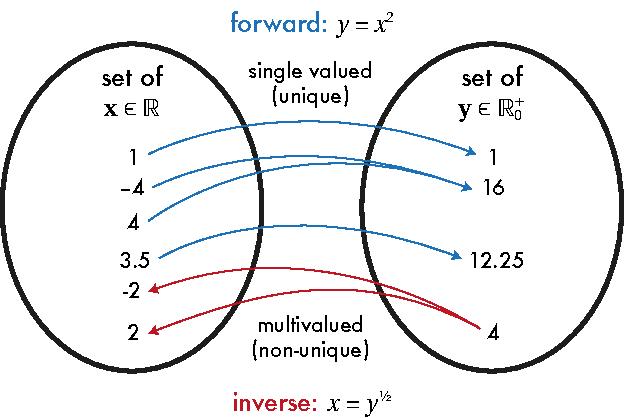
\includegraphics[]{numerical/figures/nonunique.eps}
    \caption{An example of non-uniqueness from the simple inverse of $y = x^2$.
    Solutions of $x = y^{1/2}$ are multivalued unless contrained.}
    \label{fig:nonunique}
\end{figure}

As an example of non-uniqueness, think back to our MT practical as an example where models of a conductive layer over a resistive layer shows no change in misfit (lack of sensitivity) over an extremely large range of resistivities, making them all equally likely.  In this case, the cause of non-uniqueness is a lack of sensitivity to certain model parameters due to the physics of the problem.  We can't change physics, so how can we address the ambiguity?

The shape of a misfit functional is generally smooth, but can have complexities as the model parameters change resulting in surfaces or curves that have multiple local minima (Figure~\ref{fig:misfit}).  Inversions which are iterative can get ``stuck'' within a local minima, unable to access regions with lower misfit.  Using multiple initial conditions for an inversion can occasionally help move the solution from one minima to another, but how do we tell which one is correct, certainly both cannot?  Simply choosing the lowest misfit may not be appropriate as we may be constrained by data uncertainties or the global minima may result in ``over-fitting'' the observed data.
\begin{figure}[bth]
    \centering
    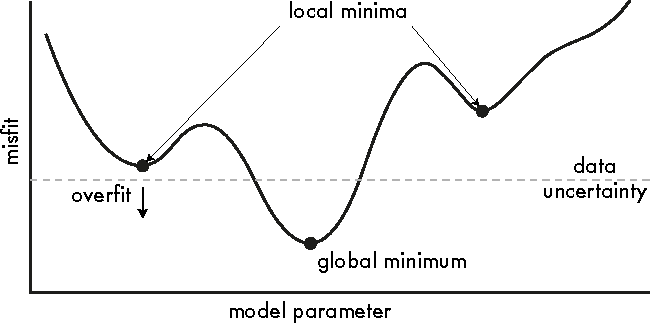
\includegraphics[]{numerical/figures/misfit_functional.pdf}
    \caption{Hypothetical misfit function.  Each point on the misfit curve
    represents a unique set of model parameters.  A misfit function may have
    multiple local minima in addition to a global minimum.  Models which sit
    below the data uncertainty overfit the data.}
    \label{fig:misfit}
\end{figure}

In some cases, it may be possible to improve sensitivity by adding data at the correct sites.  Adding additional constraints can reduce non-uniqueness, either adding another type of data with different sensitivities or geological constraints.

\subsection{Stability}
Inversion problems are notoriously unstable.  Given the wrong initial condition ``far'' from a solution may result in each successive iterative step moving increasingly further from a viable solution.  Basically the model spins out of control and the inversion will not converge.  Hence, the initial condition can affect not only the solution, but also the stability.  Another problem that can arise are models in which the values of adjacent cells increasing grow in opposite directions such that their average response at the surface may be approximately the same but the two values are increasingly divergent.  For example, imagine a resistivity cross-section that looks more like a checkerboard pattern of conductive and resistive squares rather than a geologically plausible image.  I've classified this problem as a stability issue, but it could as easily be classified as non-uniqueness as the misfit may reduce as this occurs suggesting the model fits the data but is clearly geologically implausible.

We can attempt to stabilize these problems by penalizing the misfit functional in various ways.  That is, the misfit will grow if the model strays too far from our imposed constraint in an attempt to force the inversion to take steps towards a reasonable solution rather than running away.  An analogy that sort of works is to imagine a goat tethered to a tree.
\footnote{This analogy comes from a very Russian professor, Mikhail Zhdanov, I had as a graduate student at the University of Utah.  Most of us would probably think of a tethered dog, but a goat somehow makes it so much more memorable.}
The goat can wander (misfit) anywhere between the tree and the maximum length of the rope (penalty); assuming of course that the goat doesn't eat the rope or the tree (we can only take analogies so far).  Adding these penalties doesn't always work, but it does tend to significantly improve the stability.

There are a number of misfit penalties that we can apply and we will discuss a few in greater detail in Section~\ref{sec:misfit}.  A penalty for straying too far from a prescribed model is perhaps the most closely aligned with our goat on a rope analogy.  This type of penalty best prevents the instabilities that allow models which cause misfit to grow uncontrollably.  To limit the ``checkerboard'' problem above, we can penalize the model roughness, forcing models to be smoothly varying.  The price we pay for smoothing is a difficulty in resolving boundaries that represent a step change in a model property (e.g., seismic velocity contrast between two layers).  However, there are additional method to still allow for discontinuities under certain conditions.

In addition to the stability concerns addressed above, inversions can be made unstable by the presence of a data outlier or even perhaps the smaller noisy variations in the data resulting from measurement uncertainties.  This effect can be mitigated by weighting the data by its certainty (inverse of the uncertainty) as we estimate the misfit.


\section{Misfit Functionals} \label{sec:misfit}

When developing a physical model, we require a way to quantify how well it reproduces the observed data relative to alternative models. In general, we seek a single scalar value that characterizes the mismatch between the data and a model. The mathematical expression of this mismatch is called the \emph{misfit}, a broad term for any metric used to discriminate between the performance of competing models. The choice of this metric can have a significant influence on the inversion results. A good inversion does not minimize misfit arbitrarily, but instead seeks a balance between fitting the data and producing a physically meaningful model. In selecting a metric, we implicitly introduce assumptions about noise, uncertainty, and the relative importance of different parts of the data.

To quantify misfit, we require a way to measure the size of differences between observed and predicted data. This quantification is typically accomplished using norms, which provide a measure of vector magnitude and, by extension, distance.

\ntextbox{Norms and Metrics in Inversion Theory}{
    To compare models and data, we need a way to measure how different two vectors are, such as the observed data and the predicted data. This idea is formalized using the concepts of distance, metrics, and norms, which are used to compute the misfit.

    \medskip
    \noindent\textbf{Metric (distance)} \\
    A metric is simply a measure of distance between two points or vectors. A valid distance function $d(\vb{x_1}, \vb{x_2})$ must satisfy four conditions:
    \begin{description}
        \item [Non-negativity:] distance must always be positive or zero, $d(\vb{x_1}, \vb{x_2}) \geq 0$
        \item [Identity:] the distance is zero only if the two points are identical, $d(\vb{x_1}, \vb{x_2}) = 0 \iff \vb{x_1} = \vb{x_2}$
        \item [Symmetry:] distance does not depend on order, $d(\vb{x_1}, \vb{x_2}) = d(\vb{x_2}, \vb{x_1})$
        \item [Triangle inequality:] the distance between two points is always shorter than or equal to going through a third point, $d(\vb{x_1}, \vb{x_3}) \leq d(\vb{x_1}, \vb{x_2}) + d(\vb{x_2}, \vb{x_3})$
    \end{description}

    \medskip
    \noindent\textbf{Norm (magnitude)} \\
    A norm measures the size or length of a vector, $\norm{\vb{x}} \geq 0$. Norms define a metric through
    \[
        d(\vb{x}, \vb{y}) = \norm{\vb{x} - \vb{y}},
    \]
    so that measuring misfit is equivalent to measuring distance between observed and predicted data.  For an expression to be a norm, it must satisfy properties analogous to those of a metric, including positivity, the triangle inequality, and an additional scaling property called homogeneity (defined previously in Section~\ref{sec:linearity}).

    \medskip
    \noindent\textbf{Common norms in inversion} \\
    Two norms are commonly used in inversion problems:
    \begin{description}
        \item [$L^2$-norm,] is simply the Euclidean distance, which you may remember as the Pythagorean distance for a 2-dimensional space,
        \[
            \norm{\vb{x}}_2 = \left( \sum_{i=1}^N x_i^2 \right)^{1/2}
            = (\vb{x}\T \vb{x})^{1/2}
        \]
        Note the subscript denotes the order of the norm.  This norm is the familiar straight-line distance and emphasizes larger differences more strongly. The $L^2$ norm is closely related to the arithmetic mean through the root-mean-square (RMS) value. This quantity is susceptible to outliers.

        \item [$L^1$-norm,] is the absolute distance
        \[
            \norm{\vb{x}}_1 = \sum_{i=1}^N \abs{x_i}
        \]
        This norm measures total deviation and is less sensitive to large outliers. It is closely related to the median in that minimizing an $L^1$ misfit yields a robust estimate of central tendency.
    \end{description}

    \medskip
    \noindent\textbf{Connection to inversion} \\
    In inverse problems, the misfit is simply the distance between observed and predicted data. 
    
    Because the $L^1$-norm penalizes deviations linearly, it is less sensitive to large outliers than the $L^2$-norm, which penalizes deviations quadratically. This property makes the $L^1$-norm useful when the data may contain outliers or non-Gaussian noise.
    
    Different choices of norm correspond to different ways of measuring the distance between the observed data $\vb{d}$ and the predicted data $\tilde{\vb{d}}$, and hence different definitions of what it means for a model to ``fit'' the data.
}{mathtool}\label{box:norm}

\subsection{Basic Misfit Functionals}

A common misfit functional\footnote{A functional is a function that takes a vector as an argument and returns a scalar value.}
based on the $L^2$-norm is the root-mean-square (RMS) misfit,
\begin{equation}
    \coreeq
    \phi_2 = \left( \frac{1}{N_d} 
        \sum_{i=1}^{N_d} (d_i - \tilde{d}_i)^2 \right)^{1/2},
    \label{eq:rms2}
\end{equation}
where $N_d$ is the number of data points. The RMS misfit represents the average magnitude of the residuals and corresponds to the root-mean-square value of the differences between observed and predicted data. The units of RMS are the same as the units of $\vb{d}$.

While the summation form makes the contribution of each data point explicit, it is often more convenient to express the misfit in vector form. Defining the \emph{residual} vector,
\begin{equation}
    \coreeq
    \vb{r} = \vb{d} - \tilde{\vb{d}},
\end{equation}
the $L^2$ misfit can be written as
\[
    \workeq
    \phi_2 = N_d^{-1/2} \left( \vb{r}\T \vb{r} \right)^{1/2}.
\]
or simply,
\[
    \phi_2 = N_d^{-1/2} \norm{\vb{r}}_2 .
\]

An $L^1$-norm misfit is given by
\begin{equation}
    \workeq
    \phi_1 = \frac{1}{N_d} \sum_{i=1}^{N_d} \abs{d_i - \tilde{d}_i}.
    \label{eq:rms1}
\end{equation}

The $L^1$ misfit is less influenced by large residuals and is therefore commonly used in problems such as earthquake location, where robustness to outliers is important. Note that this misfit corresponds to the mean absolute deviation, not the median.

\subsection{Weighted and Normalized Misfit}

The basic misfit functionals do not account for uncertainty in the data. In practice, it is often desirable to weight the contributions of individual data points according to their uncertainties. Data with low uncertainty are given greater influence, while noisier data contribute less.

A weighted $L^2$ misfit can be written as
\begin{equation}
    \coreeq
    \phi_2 = \left( \frac{1}{N_d} 
        \sum_{i=1}^{N_d} \frac{(d_i - \tilde{d}_i)^2}{\sigma_i^2} \right)^{1/2},
\end{equation}
where $\sigma_i$ represents the standard deviation (uncertainty) of the $i$th datum.  This expression shows explicitly that each data point is weighted according to its uncertainty, with more precise measurements contributing more strongly to the misfit. In this sense, the misfit reflects both data fit and confidence in each measurement. The weighted RMS is unitless since the elements of $\vb{d}$ are normalized by their uncertainty that has the same units.

In vector form, the weighted misfit can be written as
\begin{equation}
    \workeq
    \phi_2 = N_d^{-1/2} \norm{\vb{W}_d \vb{r}}_2 ,
\end{equation}
where $\vb{W}_d$ is a diagonal weighting matrix with elements $w_{d,ii} = 1/\sigma_i$.

\subsection{$\chi^2$ Misfit}

A commonly used related measure is the chi-squared ($\chi^2$) misfit,
\begin{equation}
    \workeq
    \chi^2 = \norm{\vb{W}_d \vb{r}}_2^2
\end{equation}
Unlike the RMS misfit, the $\chi^2$ misfit is not normalized by the number of data and therefore provides an absolute measure of misfit relative to the assumed uncertainties.

Normalizing by the number of degrees of freedom yields the reduced chi-squared,
\begin{equation}
    \chi^2_\nu = {N_{d-m}}^{-1} \norm{\vb{W}_d \vb{r}}_2^2
\end{equation}
where $N_{d-m}$ is the number of degrees of freedom (number of data minus the number of model parameters, $N_d - N_m$).

In an ideal case, we expect $\chi^2_\nu \approx 1$. Values significantly less than 1 may indicate overfitting relative to the assumed uncertainties, while values greater than 1 suggest the model does not adequately explain the data within the expected noise level.  In this sense, the chi-squared misfit provides a useful criterion for assessing whether a model fits the data at an appropriate level, rather than simply minimizing the misfit.

It is important to note that not all changes to the misfit definition affect the inversion result. The weighted RMS, $\chi^2$, and reduced $\chi^2$ misfits are related by constant scaling factors and therefore yield the same model when minimized. These forms differ only in how the misfit is normalized and interpreted.

In contrast, changing from an unweighted to a weighted misfit alters the relative importance of individual data points and generally leads to a different inversion result. More broadly, different choices of norm (e.g., $L^1$ versus $L^2$) and regularization (as we'll soon see) can lead to fundamentally different models. Only changes that alter the relative weighting of residuals will change the location of the minimum; changes in overall scaling will not.

The misfit functions introduced above provide a quantitative measure of how well a model explains the observed data. In practice, inversion methods seek to minimize this misfit by adjusting the model parameters. For linear inverse problems, this leads naturally to least-squares formulations, which will be developed in the next section. However, minimizing misfit alone is generally insufficient to define a unique or stable solution. Additional constraints on the model are typically required, and these will be introduced later.


\section{Least-Squares Inversions}

\subsection{Linear Linear Least Squares (LLSQ)}\label{sec:llsq}

Fitting lines and polynomials to data is one of the most common practices for interpreting data in many fields of science.  Most of you may be familiar with the functions that are used within a spreadsheet or other program, but may not know what it is doing behind the scenes.  Fitting a line to data is an inverse problem where we use data $y$, collected at discrete values of $x$ to determine the unknown fitting paramters, slope and $y$-intercept.

Imagine we have collected number of data (N points in all) at known locations, $x = x_1,x_2,\ldots,x_N$, resulting in observations with values, $y = y_1,y_2,\ldots,y_N$.  Assuming the data appear sufficiently linear we wish to fit a single line to all the data.  We will need to determine a slope, $m_1$, and intercept, $m_0$, which are our model, i.e., $y = m_0 + m_1 x$.  Simply fitting the data by eye is not appropriate, as it does not provide a reliable way to determine the best-fitting model or quantify uncertainty in the parameters.

We could try a range of slopes and intercepts and pick the pairs systematically or randomly and determine the one which provides the minimum misfit to the data.  Testing sets of parameters in this way is called a grid search and is essentially repeated application of the forward problem.  A grid search can be useful for mapping out the misfit surface and illustrating the sensitivities to different model parameters.  However, a grid search can be very time consuming.  As the number of of parameters grows, a grid search quickly becomes intractable.  Instead, we would rather have a way to identify the best possible model in one step.  Rather than exploring the parameter space exhaustively, we seek a method that directly identifies the model that minimizes the misfit.

One approach is to directly compute the model parameters that minimize the misfit.  The method below is called the linear least squares (LLSQ) because it minimizes the misfit of the squared difference between the data and predicted data.  Suppose we collect observations at known locations $x = x_1,x_2,\ldots,x_N$.  We choose a slope, $m_1$, and intercept, $m_0$, which yield the modeled data, $\tilde{y_i}$,
\begin{align*}
    \tilde{y}_1 &= m_0 + m_1 x_1 \\
    \tilde{y}_2 &= m_0 + m_1 x_2 \\
    \vdots \\      
    \tilde{y}_N &= m_0 + m_1 x_N ,
\end{align*}
which we can generalize as $\tilde{y}_i = m_0 + m_1 x_i$, where $x_i$ and $\tilde{y}$ are the location and estimate of the $i$-th data point.  The squared misfit of the $i$-th data point is given by,
\begin{equation*}
    r_i = y_i - \tilde{y}_i .
\end{equation*}
This individual misfit can be positive or negative indicating whether the model point is below or above the measured point.  However, we care about the total misfit (unsigned distance) from each point which is given by
\begin{equation*}
    \phi^2 = \sum_{i=1}^N r_i^2 .
\end{equation*}
Note this is an $L^2$-norm.

The minimum misfit for the $i$-th data point is a model that passes through the point $(x_i, y_i)$; though the best-fitting model for all of the data may not have a zero misfit at any given observation.  Therefore, we need to identify the set of model parameters ($m_0$ and $m_1$ in this case) which collectively provides the minimum misfit to the observations.

\ntextbox{Minimizing misfit for a line}{
    Starting from the misfit for a line, writing the model prediction as
    $\tilde{y}_i = m_0 + m_1 x_i$,
    \[
        \phi^2 = \sum_{i=1}^N (y_i - \tilde{y}_i)^2 .
    \]
    A minimum requires $\phi^2$ to be stationary with respect to \emph{each}
    parameter, so both partial derivatives vanish. Differentiating once, generically,
    with the chain rule,
    \[
        \pdv{\phi^2}{m_j} = -2 \sum_{i=1}^N (y_i - \tilde{y}_i)\,\pdv{\tilde{y}_i}{m_j}
        = 0 ,
    \]
    and for a line the basis-function derivatives are just
    $\pdv{\tilde{y}_i}{m_0} = 1$ and $\pdv{\tilde{y}_i}{m_1} = x_i$.
    The two conditions therefore say the residuals are orthogonal to each basis
    function:
    \[
        \sum (y_i - \tilde{y}_i) = 0 , \qquad
        \sum (y_i - \tilde{y}_i)\, x_i = 0 .
    \]
    Expanding $\tilde{y}_i$ gives the two \emph{normal equations} (sum limits
    $1\ldots N$ dropped on intermediate steps to reduce clutter):
    \begin{equation}
        0 = \sum_{i=1}^N y_i - m_0 N - m_1 \sum_{i=1}^N x_i ,
        \label{eq:llsq-intercept}
    \end{equation}
    \begin{equation}
        0 = \sum_{i=1}^N y_i x_i - m_0 \sum_{i=1}^N x_i - m_1 \sum_{i=1}^N x_i^2 .
        \label{eq:llsq-slope}
    \end{equation}
    To determine the optimal choices of $m_0$ and $m_1$, rearrange Equation~\ref{eq:llsq-intercept} to isolate $m_0$,
    \begin{equation}
        m_0 = \frac{1}{N} \left(\sum_{i = 1}^N y_i - m_1 \sum_{i = 1}^N x_i \right) ,
        \label{eq:llsq-b2}
    \end{equation}
    and substituting into Equation~\ref{eq:llsq-slope} and we find the optimal slope, $m$,
    \begin{align*}
        0 &= \sum y_i x_i - m \sum x_i^2 
        - \frac{1}{N} \left(\sum y_i - m_1 \sum x_i \right) \sum x_i \\
        0 &= N \sum y_i x_i - m_1 N \sum x_i^2 
        - \sum y_i \sum x_i + m_1 \left(\sum x_i \right)^2 \\
        m_1 N \sum x_i^2 - m_1 \left(\sum x_i \right)^2 &=
        N \sum y_i x_i - \sum y_i \sum x_i  ,
    \end{align*}
    and finally,
    \[
        m_1 = \frac{\displaystyle N \sum_{i = 1}^N y_i x_i - \sum_{i = 1}^N y_i \sum_{i = 1}^N x_i}
        {\displaystyle N \sum_{i = 1}^N x_i^2 - \left(\sum_{i = 1}^N x_i \right)^2} . \\
    \]
    Now that we have the optimal slope, we can input the result into Equation~\ref{eq:llsq-b2},
    \begin{align*}
        m_0 &= \frac{1}{N} \left(\sum_{i=1}^N y_i - 
        \frac{\displaystyle N \sum y_i x_i 
        - \sum y_i \sum x_i}
        {\displaystyle N \sum x_i^2 - \left(\sum x_i \right)^2}
        \sum x_i \right) \\
        m_0 &= \frac{1}{N} 
        \frac{\displaystyle N \sum y_i \sum x_i^2 
        - \sum y_i \left(\sum x_i \right)^2 
        - N \sum y_i x_i \sum x_i
        + \sum y_i \left(\sum x_i\right)^2}
        {\displaystyle N \sum x_i^2 - \left(\sum x_i \right)^2} ,
    \end{align*}
    and finally,
    \[
        m_0 = \frac{\displaystyle \sum_{i=1}^N y_i \sum_{i=1}^N x_i^2 
        - \sum_{i=1}^N y_i x_i \sum_{i=1}^N x_i}
        {\displaystyle N \sum_{i=1}^N x_i^2 - \left(\sum_{i=1}^N x_i \right)^2} .
    \]
    The variance for each model parameters is estimated by
    \begin{align*}
        \sigma_{m_0}^2 &= \frac{\displaystyle \sum_{i=1}^N x_i^2 \sum_{i=1}^N \phi_i^2}
        {\displaystyle (N - 2) 
        \left[ N \sum_{i=1}^N x_i^2 - \left(\sum_{i=1}^N x_i \right)^2 \right]} , \\
        \sigma_{m_1}^2 &= \frac{\displaystyle N \sum_{i=1}^N \phi_i^2}
        {\displaystyle (N - 2) 
        \left[ N \sum_{i=1}^N x_i^2 - \left(\sum_{i=1}^N x_i \right)^2 \right]} ,
    \end{align*}

    These equations show that the optimal parameters are determined by enforcing that the residuals are uncorrelated with the model basis functions.
}{aside}\label{box:llsq}

The minimization method in Box~\ref{box:llsq} is tedious. Additionally, it is a bit difficult, though possible, to extend to polynomials as well as lines. However, all the sums and terms make it fairly cluttered.  While this scalar derivation is instructive, it quickly becomes cumbersome for more complex models. A more compact and general formulation can be obtained using linear algebra.  Consider the equations of a line now written in matrix form,
\[
    \underbrace{
        \begin{bmatrix}
            1 & x_1 \\
            1 & x_2 \\
            \vdots & \vdots \\
            1 & x_N
        \end{bmatrix}
    }_{\vb{A}}
    \underbrace{
        \begin{bmatrix}
            m_0 \\
            m_1 \\
        \end{bmatrix}
    }_{\vb{m}} =
    \underbrace{
        \begin{bmatrix}
            y_1 \\
            y_2 \\
            \vdots \\
            y_N
        \end{bmatrix}
    }_{\vb{d}} ,
\]
which we can write as simply
\[
    \vb{A} \vb{m} = \vb{d} .
\]
Solving $\vb{A}\vb{m} = \vb{d}$ directly would require inverting $\vb{A}$, i.e., $\vb{A}^{-1}$. But computing the inverse of $\vb{A}$ directly is generally not possible because $\vb{A}$ is not square. Instead, we seek a generalized inverse that provides the best-fitting solution. This generalization requires approximating the inverse of $\vb{A}$,
\[
    \vb{m} = \vb{A}^+ \vb{d} ,
\]
where $\vb{A}^+$ is the pseudo-inverse.  The end result will be the same
solution for LLSQ as above, but in matrix form.  By multiplying
both sides by the transpose of $\vb{A}$,
\[
    \vb{A}\T \vb{A} \vb{m} = \vb{A}\T \vb{d},
\]
we create a square matrix, $\vb{A}\T \vb{A}$. Assuming this matrix is nonsingular, it can be inverted, resulting in the LLSq solution
\begin{equation}
    \coreeq
    \vb{m} = (\vb{A}\T \vb{A})^{-1} \vb{A}\T \vb{d} .
    \label{eq:llsq_solution}
\end{equation}
Hence, the pseudo-inverse, $\vb{A}^+$, given by
\begin{equation}
    \coreeq
    \vb{A}^+ = (\vb{A}\T \vb{A})^{-1} \vb{A}\T ,
    \label{eq:llsq_pseudoinverse}
\end{equation}
performs the inverse that we otherwise would have done if possible.  This matrix solution is the LLSQ inversion and, as I'm sure you will agree, more compact than the purely algebraic form.

Once we have $\vb{m}$, we can then compute the pseudodata,
\[
    \vb{A} \vb{m} = \tilde{\vb{d}},
\]
and the misfit from the residuals ($\vb{r} = \vb{d} - \tilde{\vb{d}}$),
\[
    \phi = \norm{\vb{r}} .
\]

Equation~\ref{eq:llsq_solution} provides a solution, not necessarily the unique or most appropriate solution.  Different definitions of misfit and additional constraints can lead to alternative solutions that may be more meaningful or physically realistic.  For instance, the solution above does not take into account uncertainties in the data and all data are given equal weight.  It is rarely the case with real data that our uncertainties and errors are all the same.  Therefore, we need a way to incorporate these uncertainties by giving greater weight to the more certain data and less weight to the more uncertain data.

\subsection{Weighted Linear Least Squares (WLLSQ)}

In the previous section, we assumed that all data were equally reliable. In practice, measurements often have different levels of uncertainty, which must be accounted for in the inversion.

To weight the data based on their uncertainty, we redefine our misfit to include estimates of the data uncertainties,
\begin{equation}
    \phi = \norm{\vb{W}_d \vb{r}} ,
\end{equation}
where $\vb{W}_d$ with diagonals defined by $1/\sigma_i$.  To incorporate these uncertainties into the matrix formulation, we scale both sides of the forward equation, i.e.,
\begin{equation}
    \vb{W_d} \vb{A} \vb{m} = \vb{W_d} \vb{d} ,
\end{equation}
where $\vb{W_d}$ is the weighting matrix, defined by
\begin{equation}
    \vb{W_d} =
    \begin{bmatrix}
        \sigma_1^{-1} & 0 & 0 & \dots & 0 \\
        0 & \sigma_2^{-1} & 0 & \dots & 0 \\
        0 & 0 & \sigma_3^{-1} & \dots & 0 \\
        \vdots & & & \ddots & \vdots \\
        0 & 0 & 0 & \dots & \sigma_N^{-1} \\
    \end{bmatrix} .
\end{equation}
The weighting matrix is diagonal---zero everywhere except the diagonal elements---so each data point is scaled independently according to its uncertainty.  Following a similar procedure now as we did before we can show that the solution to the weighted LLSQ problem is given by
\begin{equation}
    \vb{m} = (\vb{A}\T \vb{W_d}^2 \vb{A})^{-1} \vb{A}\T \vb{W_d}^2 \vb{d} .
\end{equation}

Alternatively, if we redefine the operator matrix and data vector as
\[
    \vb{A}_w = \vb{W}_d \vb{A}, \quad \vb{d}_w = \vb{W}_d \vb{d} ,
\]
we can write the WLLSQ solution as
\[
    \vb{m} = (\vb{A}_w\T \vb{A}_w)^{-1} \vb{A}_w\T \vb{d}_w .
\]
We have implicitly rewritten the weighted misfit in terms of a scaled residual $\vb{W}_d \vb{r}$. In this formulation, the weighting can be interpreted as rescaling the data so that all measurements have comparable uncertainty, allowing the least-squares problem to retain the same algebraic form as the unweighted case (Equation~\ref{eq:llsq_solution}).

This formulation is both mathematically compact and computationally efficient. Since many modern programming languages support linear algebra operations directly (e.g., MATLAB, Python, Julia), implementing inversion methods in this form is straightforward.

\subsubsection{Model Parameter Uncertainty}

The weighted formulation allows us to estimate uncertainty in the model parameters. The covariance matrix of the model is given by
\begin{equation}
    \vb{C}_m = (\vb{A}\T \vb{W_d}^2 \vb{A})^{-1},
\end{equation}
which describes how uncertainties in the data propagate into uncertainties in the model.

The diagonal elements of $\vb{C}_m$ represent the variances of the individual model parameters,
\[
    \sigma_{m_i}^2 = (\vb{C}_m)_{ii},
\]
while the off-diagonal elements describe correlations between model parameters.  This expression generalizes the scalar uncertainty formulas derived in the previous section and provides a more complete description of model uncertainty when data have varying levels of reliability.

Once the model covariance matrix is determined, we can estimate uncertainty in each model parameter. The vector of model variances can be written compactly as
\[
    \vb{\sigma}_m^2 = \diag (\vb{C}_m),
\]
with standard deviations given by
\[
    \vb{\sigma}_m = \sqrt{\diag(\vb{C}_m)},
\]
where the square root is taken element-wise.

Assuming the parameter estimates are approximately normally distributed, a 95\% confidence interval for the $i$th model parameter can be written as
\[
    \vb{m} \pm 1.96\,\bm{\sigma}_m.
\]
This expression is interpreted component-wise, so that the confidence interval is applied independently to each model parameter.  More generally, for finite data sets, the confidence interval can be expressed using the Student's $t$-distribution,
\[
    \vb{m} \pm t_{\alpha/2,\nu} \,\bm{\sigma}_m,
\]
where $\nu = N_d - N_m$ is the number of degrees of freedom. For large $\nu$, $t_{\alpha/2,\nu} \approx 1.96$, and the normal approximation is appropriate.

These confidence intervals provide a quantitative measure of how uncertainty in the data propagates into uncertainty in the estimated model parameters.  It is important to note that these uncertainties depend on the assumed data uncertainties and the model parameterization.

It is worth noting that these expressions also reduce naturally to the unweighted case. If all data are assumed to have equal uncertainty, the weighting matrix $\vb{W}_d$ becomes the identity matrix, and the weighted formulation simplifies to the standard linear least squares result. In this case, the model covariance reduces to $\vb{C}_m = \sigma^2 (\vb{A}\T \vb{A})^{-1}$, consistent with the expressions derived previously.

\section{Constrained Inversions}

\subsection{Motivation and Types of Constraints}
Inverse models do not always return geologically realistic solutions. These unrealistic models can arise for several reasons: the mathematics may admit solutions that are not physically meaningful, the problem may be poorly determined, or the data may be contaminated by noise.  A classic example is the $\text{D}^{+}$ magnetotelluric model, which produces layers of infinite resistivity separated by infinitesimally thin layers with finite conductance. While these models satisfy the governing equations, they are not physically plausible given the properties of geologic materials.

To obtain more geologically realistic results, we must restrict the set of allowable models. Regularization provides a framework for imposing such constraints on the inversion.  Regularization modifies the inverse problem by adding a penalty term that discourages undesirable model characteristics. In practice, this means prioritizing certain features in the model, such as smoothness, small amplitude, or structural simplicity. These constraints are introduced by modifying the misfit functional to penalize specific behaviors.  The table below lists a few of the ways such constraints are added.
\begin{table}
    \centering
    \caption{Methods for adding constraints to inversions.}
    \label{tab:regularization}
    \begin{tabularx}{\textwidth}{@{}lcXX@{}}
        \toprule
        \textbf{Constraint} &
        \textbf{Functional}, $\phi_m$ &
        \textbf{Effect} &
        \textbf{Typical use} \\
        \midrule
        damping (Tikhonov) &
        $\norm{\vb{m}}^2$ &
        small amplitude, minimum-energy models &
        stabilizes ill-conditioned problems, suppresses unrealistically large values \\

        smoothing &
        $\norm{\vb{L}\vb{m}}^2$ &
        smooth structure, spatial continuity, suppresses oscillations &
        suppresses noise amplification and promotes geologically continuous structure \\

        Occam &
        Section~\ref{sec:occam} &
        simplest (smoothest) model consistent with the data &
        minimizes unnecessary structure and avoids overfitting \\

        total variation &
        $\norm{\grad{\vb{m}}}_1$ &
        blocky structure, sharp boundaries, piecewise-constant models &
        imaging, fault recognition, sharp geologic boundaries \\

        focusing &
        $\norm{\vb{m}}_1$ &
        prioritizes zero values (sparsity), compact anomalies &
        localized targets, compact sources, parsimonious models \\

        minimum structure &
        $\sum_i \frac{m_i^2}{m_i^2 + \epsilon^2}$ &
        discrete bodies, sharp anomalies &
        ore deposits, potential fields, localized conductivity or density anomalies \\

        bounded &
        $m_{\min} \le m \le m_{\max}$ &
        constrained inversion within allowable ranges &
        positive- or negative-only values, physical property ranges, monotonicity, thermodynamic constraints \\

        coupled &
        $\grad{\vb{m}_1} \times \grad{\vb{m}_2} \approx 0$ &
        structurally similar coupled models &
        structurally correlated models, petrophysical covariance, joint inversion \\

        temporal &
        $\norm{\vb{m}_t - \vb{m}_{t-1}}^2$ &
        temporal smoothing, stable evolution &
        suppresses unrealistic temporal variability in time-lapse inversions \\
        \bottomrule
    \end{tabularx}
\end{table}

For a weighted least-squares problem, the data misfit can be written as
\[
    \phi_d(\vb{m}) = \norm{\vb{W}_d (\vb{d} - \vb{A}\vb{m})}_2^2.
\]

Previously we have focused on the misfit provided by the data $\phi_d$.  Regularization introduces an additional penalty term, $\phi_m$, leading to an objective function of the form
\begin{equation}
    \coreeq
    \Phi(\vb{m}) = \phi_d(\vb{m}) + \lambda \phi_m(\vb{m}) , 
\end{equation}
where $\lambda$ is the regularization hyperparameterthat controls the trade-off between fitting the data and satisfying the model constraints. The choice of $\phi_m$ depends on the desired characteristics of the model.


\subsection{Damping (Tikhonov regularization)}

Least-squares solutions, even when weighted by data uncertainty, do not always produce geologically reasonable models. In particular, poorly constrained parameters may take on unrealistically large values while still fitting the data adequately. Damping provides a simple and effective way to stabilize the inversion by penalizing the overall magnitude of the model parameters.

In its simplest form, damping (also known as zero-order Tikhonov regularization) penalizes deviations of the model from zero,
\[
    \phi_m(\vb{m}) = \norm{\vb{m}}_2^2.
\]
This favors minimum-energy solutions and suppresses large-amplitude features that are not required by the data.

More generally, it is often preferable to damp the model relative to an \textit{a priori}\footnote{The Latin \textit{a priori} means ``from what is earlier'' and is frequently used in statistics and sciences to mean prior knowledge.  In this case the \textit{a priori} model may be based on prior assumptions or genuine knowledge about a system (reference model), or it could simply be a simple model like a uniform half-space.}
or reference model, $\vb{m}_\text{ref}$, rather than zero. In this case, the model penalty is written as
\[
    \phi_m(\vb{m}) = \norm{\vb{m} - \vb{m}_\text{ref}}_2^2,
\]
which encourages solutions that remain close to the reference model unless the data demand otherwise. The Russian professor who taught me inverse theory used the analogy of a goat tethered to a stake to describe this form of regularization. The goat may wander freely, but the farther it moves from the stake, the stronger the restoring force becomes. In this sense, damping penalizes deviation from the reference model rather than imposing a hard constraint.

Using the weighted least-squares formulation introduced earlier, the regularized objective function becomes
\begin{equation}
    \workeq
    \Phi(\vb{m}) = \underbrace{\norm{\vb{r}_w}_2^2}_{\phi_d} + \lambda \underbrace{\norm{\vb{m} - \vb{m}_\text{ref}}_2^2}_{\phi_m},
\end{equation}
where $\lambda$ controls the strength of the damping relative to the data misfit.

Minimizing this objective function yields the normal equations
\[
    (\vb{A}_w\T \vb{A}_w + \lambda \vb{I}) \vb{m} =
    \vb{A}_w\T \vb{d}_w + \lambda \vb{m}_\text{ref}.
\]
The additional term $\lambda \vb{I}$ stabilizes the inversion and suppresses large model amplitudes, particularly in poorly constrained problems.

Solving for the model parameters gives
\begin{equation}
    \workeq
    \vb{m} = (\vb{A}_w\T \vb{A}_w + \lambda \vb{I})^{-1}
    \left(
        \vb{A}_w\T \vb{d}_w + \lambda \vb{m}_\text{ref}
    \right).
\end{equation}

\subsection{Smoothing}

Least-squares solutions, even when stabilized by damping, can still exhibit unrealistic spatial variability. In many inverse problems, especially those involving distributed Earth properties, the data do not contain sufficient information to resolve sharp variations between neighboring model parameters. As a result, small-scale oscillations may appear in the solution that fit the data but have no geological significance.

Smoothing constraints address this problem by penalizing spatial variability in the model rather than its overall magnitude. In effect, smoothing expresses the assumption that subsurface properties vary gradually unless the data provide strong evidence otherwise. This reflects both geological expectation and the limited resolving power of most geophysical measurements.

Smoothing is introduced by defining a model penalty that measures roughness rather than amplitude. In operator form, the model penalty is written as
\[
    \phi_m(\vb{m}) = \norm{\vb{L}\vb{m}}_2^2,
\]
where $\vb{L}$ is a discrete derivative operator that measures spatial variation in the model.

Using the weighted least-squares formulation introduced earlier, the regularized objective function becomes
\begin{equation}
    \Phi(\vb{m}) = \norm{\vb{r}_w}_2^2 + \lambda \norm{\vb{L}\vb{m}}_2^2.
\end{equation}

Minimizing this objective function yields the normal equations
\[
    (\vb{A}_w\T \vb{A}_w + \lambda \vb{L}\T \vb{L}) \vb{m}
    = \vb{A}_w\T \vb{d}_w,
\]
with solution
\begin{equation}
    \vb{m} = (\vb{A}_w\T \vb{A}_w + \lambda \vb{L}\T \vb{L})^{-1}
    \vb{A}_w\T \vb{d}_w.
\end{equation}

Compared with damping, smoothing replaces the identity matrix with $\vb{L}\T\vb{L}$, so that the penalty acts on spatial derivatives of the model rather than on the model itself.

Conceptually, smoothing corresponds to penalizing derivatives of a continuous model. A first-derivative (gradient) penalty can be written as
\begin{equation}
    \phi_m(m) = \int \norm{\grad m(\vb{x})}^2 \, \dd{\vb{x}},
\end{equation}
which discourages rapid spatial changes and promotes smoothly varying structure.

A second-derivative (curvature) penalty takes the form
\begin{equation}
    \phi_m(m) = \int \norm{\laplacian m(\vb{x})}^2 \, \dd{\vb{x}},
\end{equation}
which suppresses variations in gradient and produces even smoother models.

These expressions are useful for understanding the intent of smoothing constraints, but they are not evaluated directly in numerical inversions.

In practice, the model is discretized into a finite set of parameters,
\[
    \vb{m} = \begin{bmatrix} m_1 & m_2 & \cdots & m_N \end{bmatrix}\T,
\]
and spatial derivatives are approximated using finite differences (Chapter~\ref{ch:finitediff}).

A first-derivative (gradient) operator can be written as
\begin{equation}
    \vb{L}_1 =
    \begin{bmatrix}
        -1 & 1 & 0 & \cdots & 0 \\
        0 & -1 & 1 & \cdots & 0 \\
        \vdots & & \ddots & \ddots & \vdots \\
        0 & \cdots & 0 & -1 & 1
    \end{bmatrix},
\end{equation}
with corresponding penalty
\[
    \phi_m = \norm{\vb{L}_1 \vb{m}}_2^2,
\]
which penalizes differences between adjacent model parameters and promotes piecewise smooth structure.

A second-derivative (curvature) operator can be written as
\begin{equation}
    \vb{L}_2 =
    \begin{bmatrix}
        1 & -2 & 1 & 0 & \cdots & 0 \\
        0 & 1 & -2 & 1 & \cdots & 0 \\
        \vdots & & \ddots & \ddots & \ddots & \vdots \\
        0 & \cdots & 0 & 1 & -2 & 1
    \end{bmatrix},
\end{equation}
with penalty
\[
    \phi_m = \norm{\vb{L}_2 \vb{m}}_2^2.
\]
Second-derivative smoothing suppresses curvature and typically produces smoother models than first-derivative constraints.

In higher dimensions, analogous finite-difference operators are constructed for each spatial direction, and the total smoothing constraint is formed by combining the corresponding operators.

The choice between first- and second-derivative smoothing has important consequences for the resulting model. First-derivative smoothing allows linear trends and gradual changes, whereas second-derivative smoothing strongly suppresses curvature and produces very smooth models.

In both cases, smoothing reflects the limited resolving power of geophysical data. Sharp boundaries may exist in the Earth, but the data often cannot locate them precisely. Smoothing therefore represents a statement about what the data can reliably resolve, rather than a claim about the true structure of the subsurface.

This perspective provides a natural bridge to Occam inversion, which formalizes the idea of selecting the simplest model—often the smoothest—that is consistent with the data.

\subsection{Choosing the Regularization Parameter, $\lambda$}

Regularization introduces an additional degree of freedom into the inverse problem through the parameter $\lambda$, which controls the trade-off between fitting the data and enforcing model constraints. Small values of $\lambda$ prioritize data fit and may produce rough or unstable models, while large values emphasize model smoothness at the expense of fitting the observations.

There is no single universally optimal choice of $\lambda$, but several strategies exist to guide its selection.

A common diagnostic tool is the \emph{L-curve}, which plots the model penalty $\phi_m(\vb{m})$ against the data misfit $\phi_d(\vb{m})$ for a range of $\lambda$ values. Such plots often form an L-shaped curve, reflecting a trade-off between data fit and model complexity. The corner of the L-curve corresponds to a solution that balances these competing objectives and is often taken as a reasonable choice for $\lambda$.

The L-curve does not provide an automatic solution, but it offers valuable insight into how sensitive the inversion is to the choice of regularization and clarifies the consequences of prioritizing either data fit or model simplicity.

Although L-curves are often used to visualize the trade-off between data misfit and model roughness, Occam inversion does not explicitly identify the corner of an L-curve as we'll see below.

\subsection{Bounded Constraints}

In many inverse problems, model parameters are subject to physical bounds, such as positivity or known limits,
\[
    \vb{m}_{\min} \le \vb{m} \le \vb{m}_{\max}.
\]
Incorporating these constraints ensures that inversion results remain physically meaningful.

Several approaches are commonly used to enforce bounded constraints.

1.\; One approach is to reparameterize the model so that the bounds are satisfied automatically. For example,
\[
    m = \exp(u)
\]
enforces positivity, while more general transformations can map unconstrained variables to bounded intervals. These transformations allow standard inversion methods to be applied but may introduce additional nonlinearity.

2.\; Alternatively, constraints can be enforced by projecting the model back into the feasible region after each update. Given a trial model,
\[
    \vb{m}_{\text{trial}} = \vb{m}_i + \Delta \vb{m},
\]
each parameter is adjusted to satisfy the bounds,
\[
    m_j =
    \begin{cases}
        m_{\min}, & m_j < m_{\min} \\
        m_{\max}, & m_j > m_{\max} \\
        m_j, & \text{otherwise}.
    \end{cases}
\]
This approach is simple and compatible with Gauss--Newton and Levenberg--Marquardt methods, although it may affect convergence near the boundaries.

3.\; More rigorous approaches treat the bounds as part of the optimization problem and solve
\[
    \min \Phi(\vb{m}) \quad \text{subject to constraints}.
\]
Methods such as active-set or interior-point algorithms modify the update step to ensure that constraints are satisfied throughout the inversion. With their rigor comes greater difficulty to implement.

Bounded constraints restrict the admissible model space and help prevent nonphysical solutions. They are particularly important in nonlinear inversion, where large updates may otherwise produce unrealistic parameter values. In practice, a balance is required between enforcing constraints and maintaining smooth convergence of the inversion.

\subsection{Occam Inversion}\label{sec:occam}

William of Occam was a 14th-century English philosopher best known for the principle known as Occam's razor: among competing explanations that are consistent with the observations, the simplest should be preferred.

Occam inversion, developed by \citet{Constable_etal1987}, formalizes this idea in the context of inverse problems. Rather than attempting to determine a single ``true'' model, the method seeks the simplest model—typically the smoothest—that is consistent with the observed data within an acceptable level of misfit.

In this sense, Occam inversion can be viewed as a systematic approach to selecting the regularization parameter. Instead of fixing $\lambda$ directly, the method specifies an acceptable data misfit, usually consistent with the expected noise level (e.g., $\chi_\nu^2 \approx 1$), and then identifies the smoothest model that satisfies this criterion.

Although L-curves are often used to visualize the trade-off between data misfit and model roughness, Occam inversion does not explicitly identify the geometric corner of an L-curve. Instead, the solution typically lies near the L-curve corner as a consequence of enforcing the misfit criterion, rather than as the result of a curvature optimization.

Although Occam inversion is often introduced as a constrained optimization problem,
\begin{equation}
    \min_{\vb{m}} \; \norm{\vb{L}\vb{m}}_2^2
    \quad \text{subject to} \quad
    \phi_d(\vb{m}) = \phi_d^*,
\end{equation}
it is typically implemented by solving a sequence of regularized least-squares problems with different values of the regularization parameter $\lambda$.

Specifically, for a given value of $\lambda$, the model is obtained by minimizing the penalized objective function
\begin{equation}
    \Phi(\vb{m}) =
    \norm{\vb{W}_d(\vb{d} - \vb{A}\vb{m})}_2^2
    + \lambda \norm{\vb{L}\vb{m}}_2^2,
\end{equation}
which leads to the linear system
\begin{equation}
    (\vb{A}_w\T \vb{A}_w + \lambda \vb{L}\T \vb{L}) \vb{m}
    = \vb{A}_w\T \vb{d}_w.
\end{equation}
The Occam method was originally formulated with $\phi{m}$ determined using roughness, but in theory a wide variety of formulations are possible.

The resulting model $\vb{m}(\lambda)$ has an associated data misfit $\phi_d(\vb{m}(\lambda))$ and model roughness $\phi_m(\vb{m}(\lambda))$. Occam inversion proceeds by adjusting $\lambda$ until the data misfit satisfies the target criterion
\begin{equation}
    \phi_d(\vb{m}) \approx \phi_d^*,
\end{equation}
where $\phi_d^*$ is typically chosen so that the reduced chi-squared statistic satisfies $\chi_\nu^2 \approx 1$.

From this perspective, Occam inversion can be viewed as an automated procedure for selecting $\lambda$ based on a statistically meaningful misfit criterion.

In practice, this is achieved using an iterative search over $\lambda$, for example:
\begin{enumerate}
    \item Choose an initial value of $\lambda$.
    \item Solve the regularized least-squares system for $\vb{m}(\lambda)$.
    \item Evaluate the resulting data misfit $\phi_d(\vb{m}(\lambda))$.
    \item If $\phi_d > \phi_d^*$, decrease $\lambda$; if $\phi_d < \phi_d^*$, increase $\lambda$.
    \item Repeat until the misfit criterion is satisfied within a specified tolerance.
\end{enumerate}

This procedure yields the smoothest model that fits the data to the prescribed level and avoids the ambiguity associated with selecting the corner of an L-curve explicitly. The Occam solution typically lies near the L-curve corner, but this location is a consequence of the misfit constraint rather than a geometric optimization of the curve itself.

The resulting model is not unique, but it avoids unnecessary structure and provides a stable and interpretable solution. This formulation highlights a key principle of inversion: the goal is not to determine a unique model, but to identify a class of models that balance data fit and model simplicity.

The Occam inversion method is widely used in geophysical applications, particularly in electromagnetic and seismic inversion, where smooth models often provide the most reliable representation of subsurface structure.


\section{Non-linear Inverse Problems}

A forward problem is nonlinear when it does not satisfy the conditions of linearity.   In geophysics, many inverse problems are nonlinear, not necessarily because the governing physics is complex, but because model parameters influence the observations in a nonlinear manner.   Common sources of nonlinearity include:
\begin{description}
    \item [Geometry:]
    When observations depend on the spatial location, shape, or extent of structures, such as depths to interfaces or source positions. Geometry is often the dominant source of nonlinearity in geophysical problems.

    \item [Boundary conditions:]
    When the behavior of a field depends on unknown or changing boundaries, such as topography, layer interfaces, or free surfaces.

    \item [Parameter coupling:]
    When two or more parameters influence the data in a multiplicative or otherwise inseparable way, making it impossible to isolate their individual effects directly.

    \item [Nonlinear physical laws:]
    When the governing equations themselves are nonlinear in the parameters of interest, such as velocity-dependent ray paths or temperature-dependent material properties.

    \item [Implicit parameter dependence:]
    When model parameters affect the data indirectly through intermediate quantities, such as paths, sensitivities, or state variables that themselves depend on the model.
\end{description}

Unlike linear problems, nonlinear inverse problems cannot be solved in a single step. Instead, they are addressed through iterative methods that progressively refine a model estimate.

\subsection{Linearization}

In some cases, nonlinear relationships can be transformed into linear ones.  These transforms allow us to then solve for the transformed model parameters using linear least squares and solved in a single step.  Then to find the model parameters one simply needs to perform the inverse transform.

For example, if we wish to model electrical conductivity measurements on a rock at several temperature conditions, we typically us the following non-linear equation:
\begin{equation*}
    \sigma = \sigma_0 \exp \left( -\frac{H} {kT} \right) ,
\end{equation*}
where $\sigma_0$ and $H$ are unknown model parameters, $T$ is controlled, and $\sigma$ is the data.  We can transform the non-linear equation above into a linear equation by simply taking the natural logarithm of both sides,
\begin{align*}
    \log \sigma &= \log \left[ \sigma_0\exp \left( -\frac{H} {kT} \right) \right] \\
    \underbrace{\log \sigma}_{y} &= \underbrace{\log \sigma_0}_{m_0} - \underbrace{\frac{H}{k}}_{m_2} \underbrace{T^{-1}}_{x} .
\end{align*}
By redefining one of our model parameters as above, we achieve a
linear equation that can be solved using an LLSQ approach. Note that in this example, we find that the values for $H$ and $k$ are not independent.\footnote{While $H$ and $k$ are not independent, $k$ is the Boltzmann constant so we can actually determine $H$ in this case.}

However, most nonlinear problems cannot be linearized analytically.  More generally, nonlinear forward problems are linearized locally about a reference model using a first-order Taylor expansion,
\[
    \Fop(\vb{m}) \approx \Fop(\vb{m}_i)
    + \vb{J}(\vb{m}_i)(\vb{m} - \vb{m}_i),
\]
where $\vb{J}$ is the Jacobian matrix. This linear approximation is valid only in the neighborhood of $\vb{m}_i$, motivating the use of iterative solution methods.

\subsection{Gauss--Newton Method}\label{sec:newton}

Newton's method provides a general framework for minimizing nonlinear objective functions by locally approximating them with a quadratic. The Gauss--Newton method is a practical approximation of Newton's method that avoids explicit evaluation of second derivatives while retaining much of its efficiency.

The Gauss--Newton step can be interpreted in two equivalent ways. 
In the first, the objective function is approximated locally by a quadratic and the minimum of this approximation defines the update.  In the second, the method seeks the root of the gradient, $\grad \Phi = 0$, by applying Newton--Raphson to the gradient itself. 
These two perspectives lead to identical update equations but offer different geometric interpretations (Figure~\ref{fig:gauss_newton}).

For a weighted least-squares objective function,
\[
    \Phi(\vb{m}) = \norm{\vb{W}_d (\vb{d} - \Fop(\vb{m}))}_2^2,
\]
the Gauss--Newton method proceeds by linearizing the forward problem about the current model $\vb{m}_i$.

Letting
\[
    \tilde{\vb{d}} = \Fop(\vb{m}_i), \quad
    \vb{r} = \vb{d} - \tilde{\vb{d}},
\]
and defining the Jacobian
\[
    J_{ij} = \pdv{d_i}{m_j},
\]
the forward problem can be approximated as
\[
    \vb{d} \approx \tilde{\vb{d}} + \vb{J} \, \Delta \vb{m}.
\]

Minimizing the objective with respect to $\Delta \vb{m}$ leads to the linear system
\begin{equation}
    (\vb{J}\T \vb{W}_d^2 \vb{J}) \, \Delta \vb{m}
    = \vb{J}\T \vb{W}_d^2 \vb{r}.
    \label{eq:gn_basic}
\end{equation}

The model is then updated according to
\[
    \vb{m}_{i+1} = \vb{m}_i + \Delta \vb{m}.
\]

\medskip
\noindent\textbf{Role of the Jacobian} \\

The Jacobian matrix plays a central role in nonlinear inversion. Its elements,
\[
    J_{ij} = \pdv{d_i}{m_j},
\]
measure how each datum responds to a change in each model parameter.

\begin{itemize}
    \item Each \emph{row} of $\vb{J}$ describes how a single observation depends on all model parameters.
    \item Each \emph{column} describes how a single parameter influences all data.
\end{itemize}

In this sense, the Jacobian generalizes the forward operator $\vb{A}$ from linear inversion, but is evaluated at the current model and therefore changes during the inversion.

Because $\vb{J}$ depends on $\vb{m}_i$, the Gauss--Newton method solves a sequence of linearized inverse problems, updating the sensitivities at each iteration.

\medskip
\noindent\textbf{Weighted formulation} \\

In practice, data are weighted by their uncertainties. Defining
\[
    \vb{J}_w = \vb{W}_d \vb{J}, \qquad
    \vb{r}_w = \vb{W}_d \vb{r},
\]
Equation~\ref{eq:gn_basic} becomes
\[
    (\vb{J}_w\T \vb{J}_w) \, \Delta \vb{m}
    = \vb{J}_w\T \vb{r}_w,
\]
which has the same form as the weighted least-squares solution derived earlier, but now applies to a locally linearized problem.

\medskip
\noindent\textbf{Interpretation} \\

The Gauss--Newton method can be interpreted as solving a sequence of linear least-squares problems, each constructed from a local approximation to the nonlinear forward model. When the objective function is well approximated by a quadratic near the current model, the method converges rapidly. However, when the approximation is poor, the update may overshoot or converge to an unintended minimum, motivating the use of damping, regularization, or step-size control in practice.

\ntextbox{Extended derivation of the Gauss--Newton method}{
    Newton's method approximates the objective function locally by a quadratic in model space and computes a model update that aims to reach the local minimum in a single step. This large-step behavior can be efficient when the approximation is accurate, but it can also be unstable and may cause the solution to overshoot or converge to a different minimum.  In contrast, steepest descent (Section~\ref{sec:steepest})methods use only gradient information and take smaller steps, making them more stable but often slower to converge.  The Gauss--Newton method is an approximation of Newton's method, which we'll get to towards the end of the derivation.

    \medskip
    \noindent\textbf{Newton's Method} \\
    We start by expanding the objective function, $\Phi(\vb{m} + \Delta \vb{m})$, using a Taylor series about the current model $\vb{m}$:
    \[
        \Phi(\vb{m}+\Delta \vb{m}) =
        \Phi(\vb{m})
        + \pdv{\Phi}{\vb{m}}\T \Delta\vb{m}
        + \frac{1}{2} \Delta\vb{m}\T \pdv[2]{\Phi}{\vb{m}} \Delta\vb{m}
        + \varepsilon.
    \]

    Here, the first derivative corresponds to the gradient of the objective function,
    \[
        \pdv{\Phi}{\vb{m}} = \grad_{\vb{m}} \Phi(\vb{m}) =
        \begin{bmatrix}
            \pdv{\Phi}{m_1} \\
            \vdots \\
            \pdv{\Phi}{m_M}
        \end{bmatrix} .
    \]
    where $\grad_{\vb{m}}$ denotes the gradient with respect to the model parameters.  For the remaining derivation, we'll revert to $\grad$ as it is standard notation.  The second derivative defines the Hessian matrix,
    \[
        \pdv[2]{\Phi}{\vb{m}} = \vb{H} =
        \begin{bmatrix}
            \pdv{\Phi}{m_1}{m_1} & \cdots & \pdv{\Phi}{m_1}{m_M} \\
            \vdots & \ddots & \vdots \\
            \pdv{\Phi}{m_M}{m_1} & \cdots & \pdv{\Phi}{m_M}{m_M}
        \end{bmatrix}.
    \]

    Neglecting higher-order terms, the Taylor expansion becomes
    \[
        \Phi(\vb{m} + \Delta\vb{m})
        \approx
        \Phi(\vb{m})
        + \grad\Phi\T \Delta\vb{m}
        + \frac{1}{2} \Delta\vb{m}\T \vb{H} \Delta\vb{m}.
    \]

    Newton's method chooses $\Delta\vb{m}$ to minimize this quadratic approximation. Taking the derivative with respect to $\Delta\vb{m}$ gives
    \[
        \grad \Phi + \vb{H} \Delta\vb{m} = 0,
    \]
    so that
    \[
        \Delta\vb{m} = - \vb{H}^{-1} \grad \Phi.
    \]
    The update is therefore
    \begin{equation}
        \vb{m}_{i+1} = \vb{m}_i + \Delta\vb{m}
        = \vb{m}_i - \vb{H}^{-1} \grad \Phi.
        \label{eq:newton_update}
    \end{equation}

    \medskip
    \noindent\textbf{Gradient and Hessian for least-squares objectives} \\
    Let the objective function be
    \[
        \Phi(\vb{m}) = \norm{\vb{r}}_2^2 = \vb{r}\T \vb{r},
    \]
    where $\vb{r} = \vb{d} - \vb{f}(\vb{m})$.  While we typically express the forward problem as
    \[
        \tilde{\vb{d}} = \Fop(\vb{m}),
    \]
    where $\Fop$ is a (generally nonlinear) operator. For the purpose of differentiation, it is convenient to express this operator in component form,
    \[
        \vb{f}(\vb{m}) =
        \begin{bmatrix}
            f_1(\vb{m}) \\
            \vdots \\
            f_N(\vb{m})
        \end{bmatrix}
        \equiv \Fop(\vb{m}).
    \]

    Taking the gradient,
    \[
        \grad \Phi = -2 \pdv{\vb{f}}{\vb{m}}\T \vb{r}.
    \]

    The Jacobian is defined as
    \[
        \vb{J} = \pdv{\vb{f}}{\vb{m}} = 
        \begin{bmatrix}
            \pdv{f_1}{m_1} & \cdots & \pdv{f_1}{m_M} \\
            \vdots & \ddots & \vdots \\
            \pdv{f_N}{m_1} & \cdots & \pdv{f_N}{m_M}
        \end{bmatrix},
    \]
    so that
    \[
        \pdv{\vb{r}}{\vb{m}} = -\vb{J}.
    \]
    Now using the Jacobian,
    \begin{equation}
        \grad \Phi = -2 \vb{J}\T \vb{r}.
        \label{eq:grad_obj}
    \end{equation}
    Differentiating again gives the Hessian,
    \[
        \vb{H}
        = 2 \vb{J}\T \vb{J}
        + 2 \sum_{i=1}^N r_i \vb{H}_i,
    \]
    where $(\vb{H}_i)_{jk} = \pdv{r_i}{m_j}{m_k}$ is the second derivative of the residuals.  The first term ($\vb{J}\T \vb{J}$) represents curvature arising from data sensitivities, while the second term reflects nonlinear curvature of the forward model itself.

    \medskip
    \noindent\textbf{Gauss--Newton approximation} \\
    The Gauss--Newton method adds an approximation to the Hessian.  The Hessian is expensive to compute and includes second derivatives of the forward model, which are often difficult to evaluate accurately and can amplify noise.  For these reasons, it is common to approximate the Hessian using only first-derivative information.

    Near a solution, the residuals are small, $r_i \approx 0$, and the second term becomes negligible.  This assumption results in the Gauss--Newton approximation for the Hessian, i.e.,
    \begin{equation}
        \vb{H} \approx 2 \vb{J}\T \vb{J}.
        \label{eq:hessian}
    \end{equation}
    If the residuals are exactly linear in the parameters, then
    \[
        \pdv{r_i}{m_j}{m_k} = 0,
    \]
    and the approximation becomes exact.

    Substituting Equations~\ref{eq:grad_obj} and \ref{eq:hessian} into the Newton update (Equation~\ref{eq:newton_update}) yields
    \[
        \Delta \vb{m} = (\vb{J}\T \vb{J})^{-1} \vb{J}\T \vb{r}.
    \]
    This result shows that each iteration of a nonlinear inversion reduces to solving a linear least-squares problem using the current model as a reference.  Finally,
    \[
        \vb{m}_{i+1} = \vb{m}_i + \Delta \vb{m}.
    \]

    \medskip
    \noindent\textbf{Adding Weights}\\
    As before, we can add weights to the formulation.  Since the weighting matrix does not depend on the model parameters, it enters the derivation as a constant scaling, allowing us to define
    \[
        \vb{J}_w = \vb{W}_d \vb{J}, \quad
        \vb{r}_w = \vb{W}_d \vb{r}.
    \]
    This transform results in the weighted Gauss--Newton model update,
    \[
        \Delta \vb{m} = (\vb{J}_w\T \vb{J}_w)^{-1} \vb{J}_w\T \vb{r}_w.
    \]
}{core}\label{box:newton}

\subsubsection{Regularized Gauss--Newton Method}

Including regularization, the Gauss--Newton update is obtained by minimizing
\[
    \Phi(\vb{m}) = \norm{\vb{W}_d(\vb{d} - \Fop(\vb{m}))}_2^2
    + \lambda \norm{\vb{L}(\vb{m} - \vb{m}_\text{ref})}_2^2.
\]

Linearizing about $\vb{m}_i$ leads to the system
\[
    (\vb{J}\T \vb{W}_d^2 \vb{J} + \lambda \vb{L}\T \vb{L}) \Delta \vb{m}
    = \vb{J}\T \vb{W}_d^2 (\vb{d} - \vb{d}_m)
    - \lambda \vb{L}\T \vb{L}(\vb{m}_i - \vb{m}_\text{ref}),
\]
with update $\vb{m}_{i+1} = \vb{m}_i + \Delta \vb{m}$.

This formulation provides a unified framework for many inversion methods. By appropriate choices of the regularization parameter $\lambda$ and operator $\vb{L}$, a wide range of inversion strategies can be recovered. For example, setting $\lambda = 0$ yields the standard Gauss--Newton method, while choosing $\vb{L} = \vb{I}$ gives a damped (Tikhonov) formulation. More complex operators enforce smoothness or other structural constraints.

Methods such as Occam inversion operate within this same framework but determine $\lambda$ by enforcing a target data misfit rather than prescribing its value directly. In contrast, algorithms such as the Levenberg--Marquardt method introduce a damping parameter for numerical stability and step control, while steepest-descent methods use only gradient information and omit the approximate Hessian entirely. Thus, the regularized Gauss--Newton formulation serves as a central unifying structure from which many inversion strategies can be understood.

\subsubsection{Computing the Jacobian in Practice}

The Jacobian matrix plays a central role in nonlinear inversion, as it describes how small changes in model parameters affect the predicted data. For complex geophysical forward problems, however, computing the Jacobian can be one of the most expensive and technically challenging parts of an inversion. Several strategies are commonly used in practice:

\begin{description}
    \item [Analytic Jacobians:] When the governing equations are sufficiently simple, partial derivatives of the forward model with respect to the model parameters can be derived analytically. Analytic Jacobians are exact and often computationally efficient once implemented. However, deriving and maintaining analytic expressions can be difficult for complex physics, irregular geometries, or large numerical solvers.

    \item [Finite-difference Jacobians:] A widely used alternative is to approximate derivatives numerically using finite differences. The $j$th column of the Jacobian can be approximated as
    \[
        J_{ij} \approx \frac{f_i(\vb{m} + \epsilon \vb{e}_j) - f_i(\vb{m})}{\epsilon},
    \]
    where $\vb{e}_j$ is a unit vector perturbing the $j$th model parameter and $\epsilon$ is a small step size.

    Finite-difference Jacobians are straightforward to implement and require no analytic derivatives. However, they are computationally expensive, requiring one additional forward-model evaluation per model parameter, and can be sensitive to the choice of $\epsilon$.

    \item [Adjoint methods:] For large-scale problems with many model parameters, adjoint-state methods are often used to compute Jacobian-vector products efficiently. Rather than forming the full Jacobian explicitly, adjoint methods compute sensitivities with respect to all model parameters using a small number of forward and adjoint solves. While powerful, adjoint methods require careful formulation and are beyond the scope of this chapter.

    \item [Lagged or approximate Jacobians:] In many nonlinear inversions, the Jacobian does not change dramatically between successive iterations, particularly once the solution is close to convergence. In such cases, it is common to reuse the Jacobian for several iterations rather than recomputing it each time. This approach, sometimes referred to as a lagged Jacobian strategy, can significantly reduce computational cost with little impact on convergence when update steps are small.
\end{description}

The choice of Jacobian computation strategy represents a trade-off between accuracy and computational cost. Exact Jacobians improve convergence but may be prohibitively expensive, while approximate or reused Jacobians reduce cost but may slow convergence or require additional damping or regularization. In practice, the optimal strategy depends on problem size, nonlinearity, and the cost of the forward model.

Regardless of how it is computed, the Jacobian is always evaluated with respect to the current reference model, reinforcing that Gauss--Newton methods are locally valid approximations that rely on incremental updates rather than global linearity.

\subsubsection{Convergence Considerations}

Newton-type methods are locally convergent algorithms. Their success depends critically on how well the linearized approximation represents the true nonlinear relationship between model parameters and data in the neighborhood of the current estimate.

The Gauss--Newton update is derived from a first-order Taylor expansion of the forward problem about the current model estimate. As a result, the update is only reliable when the current model is sufficiently close to a solution. If the initial model is far from the true solution, the linear approximation may be poor and convergence may be slow or fail entirely.

This local nature explains why the choice of starting model is particularly important in nonlinear inversion and why multiple acceptable solutions may exist.

In its simplest form, Gauss--Newton applies the full model update
\[
    \vb{m}_{i+1} = \vb{m}_i + \Delta \vb{m},
\]
where $\Delta \vb{m}$ is obtained by solving the linearized system. In practice, however, the full update may be too aggressive and can increase the misfit rather than reduce it.

To improve stability, it is common to introduce a step-length parameter $\alpha \in (0,1]$ and apply
\[
    \vb{m}_{i+1} = \vb{m}_i + \alpha \, \Delta \vb{m}.
\]
Reducing the step length effectively increases the region over which the linear approximation is valid and can significantly improve convergence.

Regularization plays a dual role in Gauss--Newton inversion. In addition to enforcing prior model assumptions, it improves numerical stability by conditioning the system of equations that determines the model update. Increasing the regularization parameter $\lambda$ reduces the update magnitude and can prevent unstable behavior early in the inversion.

In practice, it is common to use stronger regularization in early iterations and gradually relax it as the solution approaches convergence.

Iteration is typically terminated based on one or more of the following criteria:
\begin{itemize}
    \item the data misfit falls below a prescribed threshold (e.g., $\chi_\nu^2 \approx 1$),
    \item successive model updates become small,
    \item the decrease in misfit becomes negligible,
    \item a maximum number of iterations is reached.
\end{itemize}

Because Gauss--Newton methods converge to a local minimum, satisfying a convergence criterion does not guarantee that the solution is unique or globally optimal. Instead, convergence indicates consistency between the model, the data, and the assumptions embedded in the inversion.

In geophysical applications, convergence behavior often reflects both data quality and problem geometry. Poor convergence may indicate inadequate parameterization, strong nonlinearity, insufficient data sensitivity, or an inappropriate starting model. Monitoring convergence diagnostics throughout the inversion provides valuable insight into the reliability and limitations of the resulting model.

In practice, many implementations further modify the Gauss--Newton method by introducing additional damping to control step size, leading to hybrid schemes such as the Levenberg--Marquardt method.

\subsection{Resolving Capability}
\subsubsection{Sensitivity}

Sensitivity describes how changes in model parameters influence the predicted data and therefore how strongly the data constrain different parts of the model. In nonlinear problems, sensitivity is quantified by the Jacobian matrix,
\[
    J_{ij} = \eval{\pdv{d_i}{m_j}}{\vb{m}_0},
\]
which represents the partial derivative of the $i$th datum with respect to the $j$th model parameter, evaluated at a reference model $\vb{m}_0$.

Because the Jacobian is evaluated at the current model, sensitivity in nonlinear inversion is inherently model-dependent and evolves throughout the inversion process.

The structure of the Jacobian provides direct insight into how the data constrain the model:
\begin{itemize}
    \item Each \emph{row} of $\vb{J}$ describes how a single datum depends on all model parameters.
    \item Each \emph{column} describes how a single model parameter influences all data.
\end{itemize}

Model parameters associated with small or nearly linearly dependent columns of $\vb{J}$ are weakly constrained and are particularly sensitive to noise and regularization assumptions. In contrast, parameters associated with strong, independent sensitivities are better constrained by the data.

In practice, an inversion does not recover the true model directly, but a filtered version of it. This filtering is described by the resolution matrix, which determines how structure in the true model is mapped into the estimated model.

Well-resolved parameters correspond to localized sensitivity, while poorly resolved parameters represent averages over broader regions of the model. In regions of weak sensitivity, regularization plays a dominant role in shaping the solution, meaning that different regularization choices can produce equally acceptable but structurally different models.

\subsubsection{Uncertainty}

Sensitivity controls how uncertainty in the data propagates into uncertainty in the estimated model. In the Gauss--Newton framework, the model covariance matrix is given by
\[
    \vb{C}_m = (\vb{J}_w\T \vb{J}_w + \lambda \vb{L}\T \vb{L})^{-1},
\]
showing that model uncertainty is governed by the combined effects of data sensitivity and regularization.

The diagonal elements of $\vb{C}_m$ represent the variances of individual model parameters,
\[
    \sigma_{m_i}^2 = (\vb{C}_m)_{ii},
\]
while the off-diagonal elements describe correlations and trade-offs between parameters. Poorly sensitive parameters typically exhibit large variances and strong correlations, reflecting limited constraint by the data.

\subsubsection{Resolution}

While the covariance matrix describes the uncertainty in model parameters, the resolution matrix describes how well the inversion recovers the true structure of the model. In linear inverse problems, the estimated model can be written as
\[
    \vb{m}_{\text{est}} = \vb{R} \, \vb{m}_{\text{true}},
\]
where $\vb{R}$ is the model resolution matrix. This matrix characterizes how the inversion maps the true model into the recovered model.

For a weighted and regularized problem, the resolution matrix takes the form
\[
    \vb{R} = \vb{C}_m \vb{J}_w\T \vb{J}_w.
\]

The resolution matrix provides a quantitative measure of how well individual model parameters are recovered:
\begin{itemize}
    \item If $\vb{R}$ were equal to the identity matrix, the model would be perfectly resolved.
    \item In practice, $\vb{R}$ is never the identity due to limited data, noise, and regularization.
\end{itemize}

Each \emph{row} of $\vb{R}$ describes how the estimated value of a single model parameter is influenced by the true model. A sharply peaked row indicates good resolution, while a broad row indicates that the parameter represents an average over a region of the model.

Each \emph{column} describes how a true model parameter influences multiple estimated parameters. Broad columns indicate that information is spread across the model, reflecting parameter trade-offs and limited resolving power.

Resolution is directly controlled by sensitivity and reduced by regularization. Poor sensitivity leads to a poorly conditioned system, which in turn produces a resolution matrix with broad, smeared structure.  While regularization determines how unresolved structure is distributed in the model.  Regularization improves stability but reduces resolution. Increasing $\lambda$ makes the model smoother or closer to the reference model, but also spreads information across neighboring parameters. As a result, resolved features become broader and less sharply defined.
This trade-off between stability and resolution is fundamental to inversion and reflects the limited information content of the data.

The resolution matrix provides a framework for interpreting inversion results. Well-resolved features correspond to localized structure in $\vb{R}$, while poorly resolved regions reflect averaging and parameter trade-offs. Careful interpretation requires recognizing that the recovered model is a filtered version of the true Earth, shaped by both data sensitivity and regularization.

Together, sensitivity, resolution, and uncertainty describe how the inversion extracts information from the data (Table~\ref{tab:resolve}).
\begin{table}[hbt]
    \centering
    \caption{Relationship between sensitivity, resolution, and uncertainty in inverse problems.}
    \label{tab:resolve}
    \begin{tabularx}{\textwidth}{@{}lcX@{}}
        \toprule
        Concept & Mathematical basis & Interpretation \\
        \midrule
        Sensitivity 
        & $\vb{J} = \pdv{\tilde{\vb{f}}}{\vb{m}}$ 
        & Describes how strongly predicted data respond to changes in model parameters \\

        Uncertainty 
        & $\vb{C}_m = (\vb{J}_w\T \vb{J}_w + \lambda \vb{L}\T \vb{L})^{-1}$ 
        & Quantifies confidence in model parameters and parameter correlations \\

        Resolution 
        & $\vb{R} = \vb{C}_m \vb{J}_w\T \vb{J}_w$ 
        & Describes how the true model is filtered or smeared in the recovered model \\
        \bottomrule
    \end{tabularx}
\end{table}

\subsection{Non-linear Inversion Recipes}

\subsubsection{Levenberg--Marquardt Method}

The Levenberg--Marquardt (LM) method provides a continuous transition between Gauss--Newton and steepest descent, allowing the inversion to adapt between fast convergence and stable behavior depending on the local structure of the objective function. The LM method combines the advantages of Gauss--Newton and steepest descent by introducing a damping parameter to control the magnitude and stability of the update,
\[
    (\vb{J}_w\T \vb{J}_w + \lambda \vb{I}) \, \Delta \vb{m}
    = \vb{J}_w\T \vb{r}_w.
\]

For small values of $\lambda$, the method behaves like Gauss--Newton, taking large curvature-based steps. For large $\lambda$, the system becomes dominated by $\vb{I}$, and the update approaches a scaled steepest descent step,
\[
    \Delta \vb{m} \approx \frac{1}{\lambda} \vb{J}_w\T \vb{r}_w.
\]

Thus, LM can be interpreted as a mechanism for balancing convergence speed and stability:
\begin{itemize}
    \item Small $\lambda$: fast convergence when the model is close to the solution
    \item Large $\lambda$: more stable behavior when far from the solution
\end{itemize}

In practice, $\lambda$ is adjusted adaptively during the inversion. A trial update is computed
\[
    \vb{m}_{\text{trial}} = \vb{m}_i + \Delta \vb{m},
\]
and the misfit is evaluated,
\[
    \Phi_{\text{trial}} = \Phi(\vb{m}_{\text{trial}}).
\]

If the misfit decreases, $\Phi_{\text{trial}} < \Phi_i$, the step is accepted and $\lambda$ is decreased,
\[
    \lambda \leftarrow \frac{\lambda}{\nu}.
\]
If the misfit increases, $\Phi_{\text{trial}} > \Phi_i$, the step is rejected and $\lambda$ is increased,
\[
    \lambda \leftarrow \nu \lambda,
\]
and the update is recomputed. The parameter $\nu$ is typically chosen between $2$ and $10$.

Some implementations use a gain ratio,
\[
    \rho = \frac{\text{actual decrease in }\Phi}{\text{predicted decrease}},
\]
to adjust $\lambda$ more precisely.

Compared with Gauss--Newton, the LM method is more robust for strongly nonlinear problems. Compared with steepest descent, it converges more rapidly once the solution is approached, making it one of the most widely used nonlinear inversion algorithms.

\subsubsection{Steepest Descent}

A simpler alternative to the Gauss--Newton method is steepest descent, which uses only first-derivative information. Rather than solving a linear system involving $\vb{J}\T \vb{J}$, steepest descent updates the model along the negative gradient direction,
\[
    \Delta \vb{m} = -\alpha \grad \Phi = \alpha \vb{J}_w\T \vb{r}_w,
\]
where $\alpha$ is a step-length parameter.

Thus, steepest descent avoids forming or inverting $\vb{J}\T \vb{J}$, making each iteration computationally inexpensive. However, because it does not account for curvature, convergence is typically much slower than Gauss--Newton.

Steepest descent can be interpreted as a first-order approximation to Gauss--Newton. It is often more stable, particularly when the quadratic approximation is poor, but this stability comes at the cost of slow convergence. The method is also highly sensitive to the choice of step size: if $\alpha$ is too small, convergence is slow; if too large, the inversion can become unstable.

In practice, $\alpha$ is not fixed but is adjusted adaptively to ensure that each update reduces the objective function. This is typically done using a line search, in which trial steps are evaluated and $\alpha$ is reduced until a decrease in misfit is achieved.

Two common approaches are used to select $\alpha$. In an exact line search,
\[
    \alpha = \arg\min_\alpha \Phi(\vb{m}_i + \alpha \vb{J}_w\T \vb{r}_w),
\]
which, for least-squares problems, yields
\[
    \alpha =
    \frac{\vb{r}_w\T \vb{J}_w \vb{J}_w\T \vb{r}_w}
         {\vb{r}_w\T \vb{J}_w \vb{J}_w\T \vb{J}_w \vb{J}_w\T \vb{r}_w}.
\]
Although exact, this approach is computationally expensive.

A more practical alternative is a backtracking strategy similar to the LM adjustment of $\lambda$. Starting from an initial $\alpha$, a trial model
\[
    \vb{m}_{\text{trial}} = \vb{m}_i + \alpha \vb{J}_w\T \vb{r}_w
\]
is evaluated. If $\Phi_{\text{trial}} > \Phi_i$, the step is rejected and $\alpha$ is reduced,
\[
    \alpha \leftarrow \beta \alpha,
\quad 0 < \beta < 1,
\]
and the process is repeated until a decrease is achieved. If $\Phi_{\text{trial}} < \Phi_i$, the step is accepted. Typical values are $\beta \sim 0.5$.

\begin{table}{htbp}
    \centering
    \caption{Comparision of Levenberg--Marquardt and steepest descent parameters.}
    \label{tab:inv_hyperparameters}
    \begin{tabular}{@{}lcl@{}}
        \toprule
        \textbf{Method} & \textbf{Hyperparameter} & \textbf{Interpretation} \\
        Steepest descent & $\alpha$ (step length) & step length along gradient \\
        Levenberg--Marquardt & $\lambda$ (step direction) & trust in curvature vs gradient \\
        \bottomrule
    \end{tabular}
\end{table}

\section{Bayesian Inversion}

The inversion methods developed thus far are primarily deterministic: they seek a single model that optimizes a specified objective function subject to assumptions about data uncertainty and model structure. In contrast, Bayesian inversion adopts a probabilistic framework in which all quantities are treated as random variables and the goal is to characterize the full range of models consistent with the data and prior information.

In Bayesian inversion, the solution is described by the posterior probability distribution,
\begin{equation}
    p(\vb{m} \mid \vb{d}) \propto p(\vb{d} \mid \vb{m}) \, p(\vb{m}),
\end{equation}
where $p(\vb{d} \mid \vb{m})$ is the likelihood, describing how well a model explains the data, and $p(\vb{m})$ is the prior distribution, encoding assumptions about the model before observing the data.

Assuming Gaussian data errors with covariance $\vb{C}_d$ and a Gaussian prior on the model with covariance $\vb{C}_m$, maximizing the posterior probability is equivalent to minimizing the objective function
\begin{equation}
    \Phi(\vb{m}) =
    \norm{\vb{C}_d^{-1/2}(\vb{d} - \vb{A}\vb{m})}_2^2
    + \norm{\vb{C}_m^{-1/2}(\vb{m} - \vb{m}_\text{ref})}_2^2.
\end{equation}
This expression has the same mathematical form as a weighted, regularized least-squares problem, with the data and model covariance matrices playing roles analogous to weighting and regularization operators.

From this perspective, many deterministic inversion methods—such as weighted least squares, damping, smoothing, and Occam inversion—can be interpreted as special cases of Bayesian inversion under specific assumptions about noise statistics and prior information.

Despite its conceptual appeal, fully Bayesian inversion is computationally demanding, particularly for large-scale geophysical problems, as it requires sampling or approximating high-dimensional probability distributions. Moreover, the specification of prior distributions often introduces subjective choices that may be difficult to justify or constrain.

For these reasons, Bayesian inversion methods are acknowledged here but not developed further. The deterministic approaches presented in this chapter provide practical, interpretable, and computationally efficient solutions that capture many of the essential features of Bayesian inference while remaining accessible for large geophysical inverse problems.

\section{Summary and Synthesis}

Inverse theory provides a unifying framework for relating geophysical observations to the underlying physical properties of the Earth. Throughout this chapter, we have shown how forward models describe the physics of a system, while inversion seeks to extract information about that system from incomplete and noisy data. Linear and nonlinear methods, along with regularization strategies, reveal that inversion is not simply a mathematical procedure but a structured process of balancing data, physics, and assumptions. In this way, inversion forms the conceptual backbone of geophysical interpretation, linking theory, observation, and model building.

A central theme of inversion is that solutions are neither unique nor exact. Instead, they depend on uncertainties in the data, the choice of parameterization, and the assumptions imposed through regularization. Sensitivity, uncertainty, and resolution together determine what aspects of the model are constrained by the data and which are controlled by prior assumptions. Ultimately, successful inversion requires not only solving equations but critically evaluating the reliability and meaning of the resulting models. In this sense, interpretation is inseparable from inversion, and understanding its limitations is as important as understanding its methods.

\nocite{Aster_etal2013}

\FloatBarrier
\bibliographystyle{elsarticle-harv}
\bibliography{ref}

\chapter[Inversion Theory: Advanced]{Inversion Theory\\ {\LARGE Advanced}}\label{ch:inversion2}

\section{Introduction}
In the previous chapter, we developed methods for formulating and solving inverse problems conceptually. Many of these methods reduce to solving linear systems of the form
\[
    (\vb{J}\T \vb{J} + \lambda \vb{L}\T \vb{L}) \Delta \vb{m}
    = \vb{J}\T \vb{r}.
\]
In this chapter, we focus on how to solve these systems efficiently, particularly for large-scale problems where direct methods become impractical.

\begin{table}[htbp]
    \centering
    \caption{Classification of matrix decomposition methods applied to inverse problems.}
    \label{tab:decomp}
    \begin{tabular}{@{}lcl@{}}
        \toprule
        \textbf{Category} & \textbf{Examples} & \textbf{Idea} \\
        \midrule
        Factorizations (not reduced) & LU, QR & Solve systems \\
        Low-rank decompositions & SVD, eigen & truncate spectrum \\
        Iterative subspace methods & CG, LSQR & build solution in Krylov space \\
        Explicit reduced basis & REBOCC, subspace inversion & restrict model \\
        Model reduction & POD, RBM & reduce forward model \\
        \bottomrule
    \end{tabular}
\end{table}

\section{Linear Systems in Inversion}

Inverse problems frequently reduce to solving linear systems,
\[
    \vb{A}\T \vb{A} \vb{m} = \vb{A}\T \vb{d},
\]
or, in the nonlinear case,
\[
    \vb{J}\T \vb{J} \Delta \vb{m} = \vb{J}\T \vb{r}.
\]
The properties of these systems, including conditioning and rank, strongly influence the accuracy and stability of the inversion.

\section{Direct Methods}

\subsection{LU Decomposition}

A general linear system can be solved using LU decomposition,
\[
    \vb{A} = \vb{L}\vb{U},
\]
where $\vb{L}$ is lower triangular and $\vb{U}$ is upper triangular. This allows the solution to be computed efficiently using forward and backward substitution.

\subsection{QR Decomposition}

For least-squares problems, QR decomposition is often preferred,
\[
    \vb{A} = \vb{Q}\vb{R},
\]
where $\vb{Q}$ is orthogonal and $\vb{R}$ is upper triangular. The solution is obtained from
\[
    \vb{R} \vb{m} = \vb{Q}\T \vb{d}.
\]
This approach avoids forming $\vb{A}\T \vb{A}$ and improves numerical stability.

\section{Singular Value Decomposition}

The singular value decomposition (SVD) provides a powerful framework for analyzing inverse problems,
\[
    \vb{J} = \vb{U} \boldsymbol{\Sigma} \vb{V}\T,
\]
where $\boldsymbol{\Sigma}$ contains the singular values.

\subsection{Truncated SVD}

Small singular values amplify noise and lead to unstable solutions. Truncated SVD (TSVD) mitigates this by retaining only the largest singular values,
\[
    \vb{m}_{\text{TSVD}} = \sum_{k=1}^{p} \frac{\tilde{d}_k}{\sigma_k} \vb{v}_k,
\]
providing a natural form of regularization.

\section{Iterative Methods}

\subsection{Steepest Descent Revisited}

Steepest descent provides a simple iterative solution method based on gradient information alone. While computationally efficient per iteration, convergence is often slow.

\subsection{Conjugate Gradient Method}

The conjugate gradient (CG) method provides a more efficient iterative approach for solving systems of the form
\[
    \vb{A} \vb{x} = \vb{b},
\]
particularly when $\vb{A}$ is symmetric and positive definite (e.g., $\vb{J}\T \vb{J}$).

CG constructs a sequence of conjugate search directions, allowing the solution to be found efficiently within a low-dimensional subspace. In practice, CG often converges much more rapidly than steepest descent.

\section{Reduced-Basis Methods}

For large-scale problems, reduced-basis methods limit the inversion to a lower-dimensional subspace.


\section{LU factorization}

LU factorization
\[
    \vb{A} = \vb{L}\vb{U}
\]
used to solve linear systems efficiently


\section{QR factorization}

QR factorization
\[
    \vb{A} = \vb{Q}\vb{R}
\]
used for least-squares stability

\section{Singular Value Decomposition (SVD)}

For large-scale inverse problems, forming and solving systems involving $\vb{J}$ or $\vb{J}\T \vb{J}$ can be computationally expensive. In such cases, it is often advantageous to approximate the forward operator or Jacobian using a reduced basis.

Methods such as truncated singular value decomposition (SVD) or subspace inversion represent the model or data in a smaller set of basis functions, reducing the dimensionality of the problem. These approaches effectively filter out components of the model that are poorly constrained by the data, improving computational efficiency and stability.

To use SVD of the forward operator to solve for linear or linearized inverse problems,
\[
    \vb{J} = \vb{U} \boldsymbol{\Sigma} \vb{V}\T,
\]
where $\vb{U}$ and $\vb{V}$ are orthogonal matrices and $\boldsymbol{\Sigma}$ contains the singular values.

Transforming the data into the singular vector basis,
\[
    \tilde{\vb{d}} = \vb{U}\T \vb{d},
\]
the solution can be written as
\[
    \vb{m} = \sum_{k} \frac{\tilde{d}_k}{\sigma_k} \vb{v}_k,
\]
where $\sigma_k$ are the singular values and $\vb{v}_k$ are the columns of $\vb{V}$.

In practice, small singular values amplify noise and lead to unstable solutions. A common approach is truncated SVD (TSVD), in which only the largest singular values are retained:
\[
    \vb{m}_{\text{TSVD}} = \sum_{k=1}^{p} \frac{\tilde{d}_k}{\sigma_k} \vb{v}_k,
\]
where $p$ is chosen to balance resolution and stability.

Truncated eigen-decomposition (very closely related to SVD)
If:
\[
    \vb{J}\T \vb{J} = \vb{V} \boldsymbol{\Lambda} \vb{V}\T
\]
Then keep only largest eigenvalues:
\[
    \vb{m} \approx \sum_{k=1}^{p} c_k \vb{v}_k
\]

SVD methods thus provide an alternative form of regularization by filtering poorly resolved components of the model, effectively reducing the dimensionality of the problem.

In electromagnetic applications, for example, reduced-basis techniques such as REBOCC exploit the structure of the forward operator to accelerate inversion.  While powerful, these reduced basis methods require additional mathematical development and are not treated in detail here.

\section{Congugate Gradient (CG)}

“We can't invert $\vb{J}\T \vb{J}$ explicitly anymore”
“We need iterative solvers”
“We work in subspaces”

Krylov subspace method

CG is a more efficient way to solve the same system Gauss–Newton produces.
\[
    (\vb{J}\T \vb{J}) \Delta \vb{m} = \vb{J}\T \vb{r}
\]
instead of:

forming and inverting matrices
you solve iteratively

\subsection{Subspace Inversion}

In subspace methods, the model update is represented as
\[
    \Delta \vb{m} = \vb{V}_p \boldsymbol{\alpha},
\]
where $\vb{V}_p$ contains a reduced set of basis vectors. This approach reduces computational cost and filters poorly resolved components.

\subsection{Applications}

Examples include truncated SVD and domain-specific methods such as REBOCC in electromagnetic inversion.

\section{Choosing a Computational Approach}

The choice of method depends on problem size, conditioning, and computational resources:

\begin{itemize}
    \item Small problems: direct methods (LU, QR)
    \item Moderately sized problems: QR or SVD
    \item Large-scale problems: CG or other iterative methods
    \item Ill-conditioned problems: SVD or regularized methods
\end{itemize}

\section{Summary}

Inverse problem formulations define the equations to be solved, while numerical linear algebra determines how these equations are solved in practice. For large-scale geophysical problems, the choice of computational method often determines whether an inversion is feasible at all.

\part{Math Appendices}
\appendix
\chapter{Mathematics Primer}

\begin{quote}The power of equations lies in the philosophically difficult
correspondence between mathematics, a collective creation of human minds, and an
external physical reality.  Equations model deep patterns in the outside world.
By learning to value equations, and to read the stories they tell we can uncover
vital features of the world around us.  In principle, there might be other ways
to achieve the same result.  Many people prefer words to symbols; language, too,
gives us power over our surroundings.  But the verdict of science and technology
is that words are too imprecise, and too limited, to provide an effective route
to deeper aspects of reality.  They are too coloured by human-level assumptions.
Words alone can't provide the essential insights.

Equations can.

-Ian Stewart, {\it In Pursuit of the Unknown, 2012}
\end{quote}


\section{Introduction}

Mathematics is a language not expressed in words but in symbols.  You might
start to wonder if mathematicians are an alien race with their own language or
at the very least an international cabal trying to promote a Greek as a global
language.  We use math because it is the most efficient and effective way to
portray quantitative information and ideas.  One of the beauties of mathematics
is that it is universal, by this I mean that it doesn't matter what language you
natively speak and what words you attribute to the symbols it holds the same
intrinsic meaning.  Because of its power, geophysics is awash with mathematics
and you will need a reasonable level of competence to fully grasp the concepts
in this course.

The purpose of this maths primer is to cover a great deal of the background
mathmematics that you will need to understand this course to the fullest extent
possible.  Read over them once early in the course and then refer back to
specific sections as they arise throughout the course. 

If you suffer from math-phobia---as a great number of people do---the largest
obstacles to learning math are mental blocks that are self-created.  Many
spectacular scientists are math-phobic, but have learned to resist the self
imposed limits of understanding when the need arises.  If there are math
concepts that you do not understand ask for help from myself, the demonstrators,
your peers.  There is also the Maths Learning Centre, a campus resource that
anyone can utilize.


\subsection{HELP!!! Maths Learning Centre}

Level 3 East, Hub Central, North Terrace Campus

The Maths Learning Centre (MLC) helps all students learn and use the maths they
need at uni (including statistics). They specialise in helping people improve
their confidence and skills for learning maths. The MLC offers seminars,
workshops, online and print resources and also a drop-in service.

{\bf MLC Drop-In room -- Level 3 Hub Central} \\
Staffed 10am to 4pm, Monday to Friday during teaching weeks, SWOT and exams. 
No appointment needed, come as often as you want, stay as long as you need.
Talk to a staff member about anything mathematical relating to your course.

{\bf MLC Resources for this course}
Resources to help you succeed with the maths relating to this course may be
found on the MLC website at
\url{adelaide.edu.au/mathslearning/resources/}.

For further information: \\
phone: \href{tel:+61-8-8313-5862}{8313 5862} \\
e-mail: \url{mailto:mathslearning@adelaide.edu.au} \\
web: \url{adelaide.edu.au/mathslearning/}.

\subsection{Common Symbols}

\begin{table}[hbt]
    \centering
    \caption{Greek alphabet.\vspace{2pt}}
    \label{tab:mathsym}
    \begin{tabular}{@{}clclcl@{}}
        \toprule
        Letter &
        Name &
        Letter &
        Name &
        Letter &
        Name \\
        \midrule
        $\mathrm{A}$, $\alpha$     & alpha &
        $\mathrm{I}$, $\iota$      & iota  &
        $\mathrm{P}$, $\rho$ or $\varrho$ & rho \\

        $\mathrm{B}$, $\beta$      & beta  &
        $\mathrm{K}$, $\kappa$     & kappa &
        $\Sigma$, $\sigma$     & sigma \\

        $\Gamma$, $\gamma$      & gamma &
        $\Lambda$, $\lambda$    & lambda &
        $\mathrm{T}$, $\tau$       & tau \\

        $\Delta$, $\delta$      & delta &
        $\mathrm{M}$, $\mu$        & mu &
        $\Upsilon$, $\upsilon$  & upsilon \\

        $\mathrm{E}$, $\epsilon$ or $\varepsilon$ & epsilon &
        $\mathrm{N}$, $\nu$        & nu &
        $\Phi$, $\phi$ or $\varphi$ & phi \\

        $\mathrm{Z}$, $\zeta$      & zeta  &
        $\Xi$, $\xi$            & xi &
        $\mathrm{X}$, $\chi$       & chi \\

        $\mathrm{H}$, $\eta$       & eta   &
        $\mathrm{O}$, $\mathrm{o}$    & omicron &
        $\Psi$, $\psi$          & psi \\

        $\Theta$, $\theta$ or $\vartheta$ & theta &
        $\Pi$, $\pi$            & pi &
        $\Omega$, $\omega$      & omega \\
        \bottomrule
    \end{tabular}
\end{table}

\begin{table}[hbt]
    \centering
    \caption{Other symbols.\vspace{2pt}}
    \label{tab:symbols}
    \begin{tabular}{@{}ccl@{}}
        \toprule
        \textbf{Symbol} & \textbf{Name} & \textbf{Use} \\
        \midrule
        $x$ & {} & scalar \\
        $\vb{x}$ & {} & vector\\
        $\mat{x}$ & {} & matrix \\
        $\sim$ & {} & approximately \\
        $\approx$ & {} & approximately equal to \\
        $\sum$ & sum operator & summation \\
        $\prod$ & product operator & product analogy to summation \\
        $\infty$ & {} & infinity \\
        $\to$ & goes to & used for limits \\
        $\partial$ & partial & partial derivative \\
        $d$ & infintesimal & derivatives/integration \\
        $\nabla$ & nabla or del & vector differential operator \\
        $\int$ & anti-derivative/integral & integration \\
        $\hat{}$ & hat & denotes unit vector \\
        $\dagger$ & dagger & denotes complex conjugate \\
        \bottomrule
    \end{tabular}
\end{table}

\section{Big and Small Numbers}

Sometimes the numbers we discuss get very big or very small.  As you can see
from the table below, writing out the full number can get very cumbersome---not
to mention hard to read.  Imagine haveing to count the number of zeros every
time just to see how big a number is.  Never fear, there is a shorthand.  Either
we can divide the number by a conveniently large or small number and use the SI
shorthand, or we can write the number as a power of ten (Table~\ref{tab:pot}).
\begin{table}[hbt]
    \centering
    \caption{Powers of ten.}
    \label{tab:pot}
    \begin{tabular}{@{}lcclc@{}}
        \toprule
        \textbf{name} & \textbf{SI prefix} & \textbf{SI symbol} & $10^x$ & \textbf{number} \\
        \midrule
        septillion & yotta & Y & $10^{24}$ & 1 000 000 000 000 000 000 000 000 \\
        sextillion & zetta & Z & $10^{21}$ & 1 000 000 000 000 000 000 000 \\
        quintillion & exa & E & $10^{18}$ & 1 000 000 000 000 000 000 \\
        quadrillion & peta & P & $10^{15}$ & 1 000 000 000 000 000 \\
        trillion & tera & T & $10^{12}$ & 1 000 000 000 000 \\
        billion & giga & G & $10^9$ & 1 000 000 000 \\
        million & mega & M & $10^6$ & 1 000 000 \\
        thousand & kilo & k & $10^3$ & 1 000 \\
        hundred & hecto & h & $10^2$ & 100 \\
        ten & deca & da & $10^1$ & 10 \\
        one & {} & {} & $10^0$ & 1 \\
        tenth & deci & d & $10^{-1}$ & 0.1 \\
        hundreth & centi & c & $10^{-2}$ & 0.01 \\
        thousandth & milli & m & $10^{-3}$ & 0.001 \\
        millionth & micro & $\mu$ & $10^{-6}$ & 0.000 001 \\
        billionth & nano & n & $10^{-9}$ & 0.000 000 001 \\
        trillionth & pico & p & $10^{-12}$ & 0.000 000 000 001 \\
        quadrillionth & femto & f & $10^{-15}$ & 0.000 000 000 000 001 \\
        quintillionth & atto & a & $10^{-18}$ & 0.000 000 000 000 000 001 \\
        sextillionth & zepto & z & $10^{-21}$ & 0.000 000 000 000 000 000 001 \\
        septillionth & yocto & y & $10^{-24}$ & 0.000 000 000 000 000 000 000 001 \\
        \bottomrule
    \end{tabular}
\end{table}

To write a number, $x$, as a power of ten we simply count the digits to the left
(if $x > 1$) or right (if $x < 1$) of the decimal to the most significant digit.
If $n$ is our number of digits and $x > 1$, the order is $n-1$ and $x < 1$ than
one, the order is $n$.  Examples:
\begin{align}
    12300 &= 1.23 \times 10^4 , \\
    0.0321 &= 3.21 \times 10^{-2} . \\
\end{align}

Numbers written in this manner, $a \times 10^b$, are often said to be in {\it
scientific notation}.  Beyond making large and small numbers eaiser to read, we
can use this scientific notation to simplify multiplication and division.  In
fact, you'll be encouraged to do this a number of times throughout the course as
you perform back-of-the-envelope calculations.  To multiply two numbers
expressed in scientific notation, we multiply each mantissa ($a$) and add the
exponents ($b$).  Example:
\begin{align*}
    6 \times 10^3 * 2 \times 10^{-4} = (6 \cdot 2) \times 10^{(3 + (-4))} \\
    &= 12 \times 10^{-1} \\
    &= 1.2 \times 10^{0}.
\end{align*}
As above, sometimes we need to adjust power of 10 following the operation.

Your calculator and computers often write numbers this way both because
calculations are faster and it saves memory.  However, when a calculator or
computer write scientific notation, they also tend to shorten it by $a \times
10^b$ to $a\,\mathrm{e}\,b$ or $a\,\mathrm{E}\,b$, where $\mathrm{e}$ and $\mathrm{E}$
substitute for $\times 10$. 


\section{Accuracy versus Precision}

The goal of observation is to be {\it precise} and {\it accurate}.  However, we
must be careful because they do not mean the same thing.  Precision
results from the sensistivity of an instrument or other measurement and
represents how repeatable an observation may be made.  Accuracy is being close
to the truth, although, this may be closeness in an average sense rather than as
the result of any singe observation.

It is possible to be precise and not accurate (Fig.~\ref{fig:avp}) when an
instrument is miscalibrated, your location is incorrect, or there is some other
systematic bias to the data.  In general, it is better to sacrifice precision
for accuracy if the choice must be made.
\begin{figure}
    \centering
    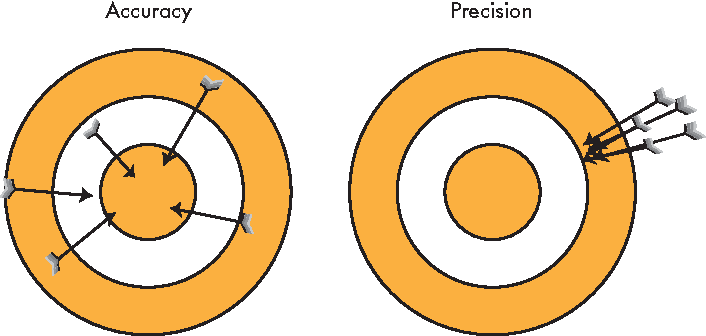
\includegraphics[]{math_primer/figures/accuracy_vs_precision.eps}
    \caption{The difference between accuracy and precision.  On the left, the
    arrows are accurate, but not precise.  Those on the right are precise, but
    not accurate.}
    \label{fig:avp}
\end{figure}


\section{Significant Digits}

Even though your computation yields a long list of digits doesn't mean we need
all of them.  For example, $5/6 = 0.8333333...$; however, we only have one
significant digit in 5 and 6, hence our answer should be written as one
significant digit as 0.8.  To determine the number of significant digits count
the number of digits between preceeding and trailing zeros.

Why do we care about significant digits?  Every instrument we use perform a
measurement has a scale.  The smallest change in a quantity the instrument can
report is the precision (e.g. the shortest distance between ticks on a ruler).
Any numbers that are reported below that number are an estimate or purely
ficticious.  We can reasonably keep one estimated digit, but all others should
be dropped.  Note: trailing zeros can be significant if our measuring device
reports a trailing zero.

As we perform mathematical operations, we should keep in mind the number of
significant digits for each of our quantities and report our answer with the
same number of significant digits as our least precise quantity.  The
significant digits of our physical constants should also be taken into an
account (although most have greater precision than our measurements).  Although,
a constant such as $2$ in our equation (e.g., kinetic energy $= \frac{1}{2} m
v^2$) can be assumed to have infinite precision (so don't round to one digit
based on it alone).

There are a couple rules for rounding (we'll use the simplist one).  Take the
last significant digit.  If it is $\geq$5, round the preceeding digit up,
otherwise truncate after the most significant digit.  An example is provided
below (Table~\ref{tab:sigdig}).
\begin{table}[hbt]
    \centering
    \caption{Significant digits for 7288.1345 to varying precision.}
    \label{tab:sigdig}
    \begin{tabular}{cl}
        \toprule
        \textbf{Significant digits} & \textbf{Rounded result} \\
        \midrule
        8 & 7288.1345 \\
        7 & 7288.135 \\
        6 & 7288.13 \\
        5 & 7277.1 \\
        4 & 7277 \\
        3 & 7280 \\
        2 & 7300 \\
        1 & 7000 \\
        \bottomrule
    \end{tabular}
\end{table}

\section{Basic Math Concepts}

\subsection{What is a function?}

In the previous section, we described a field as a function.  But what exactly is it and how do we use it in geophysics?  A function performs and operation or set of operations on an input.  Hence, for the specified domain (set of points), $x$, the function, $f$, transforms $x$ into a new domain, $y$,
\[
    x \mapsto f(x) = y.
\]

To specify the domain of $x$, we will use $[\,]$ to specify a closed domain, which includes the end-points, and $(\,)$ to specify a open domain, which excludes the end-points.  For example, suppose we use the function $f(x) = r^{-2}$ to describe some physical relationship where the domain over which it is valid lies from $0$ to $R$ but not including $R$.  In this case, we would say that $r \in [0,R)$, where $\in$ means ``is an element of.''  You might be wondering why we make a distinction between a domain that includes an end-point or not.  Some physical processes change their functional form (shape) at a boundary, yield a value different than the function would predict, or the result is undefined at a boundary.  For instance this occurs for an electric field perpendicular to a geologic boundary where the resistivity changes.

Most physical processes result in only one solution and are said to be single-valued, for each input their is exactly one output.  However, there are times the mathematical functions we use to describe a process are multi-valued, multiple possible output to a single input.  For example, the function $f(x) = x^{1/2}$ is a multi-valued function.  Because both positive and negative numbers yield a positive value when squared, the square-root is ambiguous and could yield either a positive or negative value.  Generally when we need a multi-valued function to describe a process we will add a restriction that makes it single valued.  For instance, for $f(x) = x^{1/2}$ we limit the solution to a positive result.

The above example also brings forth an important point.  The inverse to a function performs an operation, such that the identity set is returned.  As a simple example,
\[
    f[f^{-1}(x)] = x.
\]
In geophysics, we wish to understand the distribution of a particular property (or set of properties) given the response of physical effect. For gravity, it is rather simple to write down a function for gravity with a known distribution of masses.  We call this the \emph{forward problem} and is rather simple to write down as a single-valued mathematical function.  However, we measure the gravitational force or acceleration due to an unknown distribution of masses.  This formulation is the \emph{inverse problem}.  For many inverse problems, it is far more difficult to write down a single-valued function because there are often multiple valid solutions, e.g., mass distributions that can lead to the same measured data.  This nonuniqueness is especially true when the data have some level of uncertainty, which is always the case.  In this text, we begin by focusing on forward problems. In later parts of the sequence we return to inverse problems and develop more sophisticated tools to handle their non-uniqueness and instability.

\subsection{Continuity and Differentiability Definitions}

For a function to be continuous, it must not have any steps, holes (a single undefined point in an otherwise smooth function), or divergent limits.  If you were asked to draw a function and were forced to pick up the pencil, the function would be discontinuous.  A function can also be continuous but not differentiable if it has sharp corners (cusps), which commonly occur at physical boundaries leading to phenomena like refraction. We will forgo a more rigorous definition since this explanation is sufficient for our needs.

In physics, many functions become discontinuous at boundaries, but are continuous in the regions in between.  In this case, we call our functions piece-wise continuous.
\begin{center}
    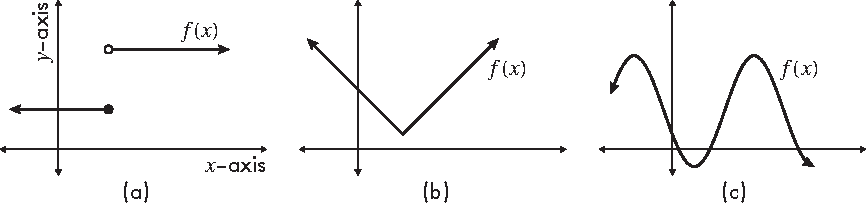
\includegraphics[]{introduction/figures/contdiff.pdf}
    \captionof{figure}{Examples of different types of functions. (a) Discontinuous or
    piecewise continuous. (b) Continuous but not differentiable. (c) Continuous
    and differentiable.}
\end{center}

A function is said to be differentiable if the derivative exists everywhere throughout its defined domain.  But again, there are locations, typically boundaries, where the derivative does not exist or only as a limit from one side.  For a function to be differentiable, it must be continuous and smoothly varying (i.e., no radical changes in slope).  A function can be continuous but not differentiable.  For example $f(x) = \abs{x}$ is continuous everywhere, but not at $x = 0$.

\clearpage
\nocite{Schey1997}

\chapter{Algebra \& Trigonometery}\label{apx:algebra}

We'll start simple and build up the complexity to give you an introduction to
some of the basic physical and mathematical concepts that we will need as part
of this course.

\section{Algebra}

While much of this particular tutorial may be review for many of you, it is
important to define the set of rules for our common language.  We will use them
as we rearrange equations on the way to identifying key geophysical
relationships.  If you aren't a math fanatic you are more than likely to find
much of this dreadfully boring (I'm actually falling asleep writing this...but
that could be because it is after midnight).  However, it is important to define
these properties as they will not be true for all operators as we move beyond
simple scalar algebra.  (Remember: a scalar is a single number value
representing a quantity at a single point in space and time).

\subsection{Order of Operations}

Take the following example:
\begin{equation*}
    2 + 3 * 5 = ?
\end{equation*}
Do we work right-to-left or left-to-right?  If we perform the sum first and the
multiplication second, we find
\begin{equation*}
    (2 + 3) * 5 = 5 * 5 = 25 .
\end{equation*}
Note I have used parentheses to specify group the sum so that it is performed
first in this case.  Let us try again, but multiply first and sum second,
\begin{equation*}
    2 + (3 * 5) = 2 + 15 = 17 .
\end{equation*}
These answers are not the same! Hence the order of operations matters.  How do
we choose the order of operations?  The rules are set by convention and the
specific ordering is given in the table below with the highest order operations
to be performed first.  Anything at the same order $+$ and $-$ for example can
be performed interchangably.  If we then follow the order of operations
appropriately, it does not matter if we work right-to-left or left-to-right in
more complex situations.

\begin{table}[hbt]
    \centering
    \caption{Operation hierarchy.\vspace{2pt}}
    \label{tab-symbols}
    \begin{tabular}{ccl}
        \toprule
        order & symbol & operation \\
        \midrule
        1 & $($ $)$, $[$ $]$, $\{$ $\}$ & grouping (inside first) \\
        2 & $a^x$, $\sqrt[x]{a}$, $\dagger$ & powers, roots, conjugation \\
        3 & *, / & multiplication and division \\
        4 & +, - & addition and subtraction \\
        \bottomrule
    \end{tabular}
\end{table}


\subsection{Operators} \label{algebra:ops}

An operation is a task or procedure that results in a new result from one or
more input parameters.  An operator is the symbol/name you instill with a
special functionality.  You are no doubt familiar with the most common
operators, $+$, $-$, $*$, $/$, representing addition, subtraction,
multiplication, and division, respectively.  But there are many others,
logarithms ($\log$) and sine ($\sin$), for example.

At the moment, we will define the properties of certain operations for scalars
and we shall see how they hold up for various systems later.  
\begin{description}
    \item[Identity element:] An operation with the identity element leaves the
    second parameter unchanged by the operation.
    \item[Inverse element:] An operation involving a parameter and its inverse
    element yield the identity element.  Basically it undoes an algebraic
    operation; a principle that is commonly employed to rearrange and/or
    simplify relations.
    \item[Commutative property:] A single operation is commutative if swapping the
    order of the parameters does not change the result.
    \item[Associative property:] When the same operator is used in succession,
    the process is associative if the result is unchanged by the order of
    operations.
    \item[Distributive property] One operator is distributive over another if 
\end{description}

\ntextbox{Real Numbers}{
    \noindent At the moment we will just concern ourselves with the set of
    real numbers, denoted $\mathbb{R}$.  Real numbers are defined as a set
    of all numbers along a continuous number line, both positive and
    negative numbers and including decimal values.  It may seem strange that
    I am defining something so seemingly simple, but as you will see later
    in the course some numbers are not part of the real set.

    \begin{center}
        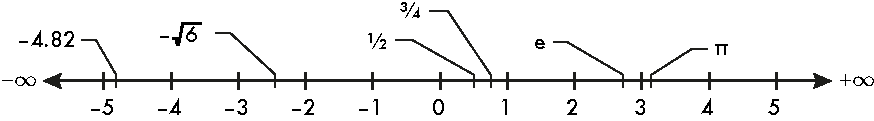
\includegraphics[]{math_primer/figures/real_number_line.pdf}

        \textbf{Figure~\thefigure:} The real number line includes the set of all integers (positive, negative, and zero), fractions, irrationals (e.g.  $\sqrt{2}$), and transcendental numbers (e.g., $\pi$ and $e$).
        \label{fig:realnum}
    \end{center}
}{mathtool}

It would be laborious and unnecessary to prove all of these properties for each
of the the various algebraic operators.  For our purposes, it is sufficient
enough to know that they work...we will leave the proving to the
mathematicians.  So without further ado, rules for addition and multiplication:
\begin{align}
    a + 0 &= a          && \quad \text{identity} \\
    a + b &= b + a      && \quad \text{commutative} \\
    a + (b + c) &= (a + b) + c && \quad \text{associative} \\
    a \cdot 1 &= a      && \quad \text{identity} \\
    ab &= ba            && \quad \text{commutative} \\
    (ab)c &= a(bc)      && \quad \text{associative} \\
    a(b + c) &= ab + ac && \quad \text{distributive}
\end{align}
It is also worthwhile to define multiple self-multiplicative operations, $aa =
a^2$ for instance.  We call these powers---or exponentials for more generally
including non-integer values---which have the properties:
\begin{align}
    a^0 &= 1            && \quad \text{by definition} \\
    a^1 &= a            && \quad \text{identity} \\
    (ab)^c &= a^c b^c   && \quad \text{distributive} \\
    a^b a^c &= a^{(b + c)} && \quad \text{distributive} \\
    (a^b)^c &= a^{(bc)} .
\end{align}
Note the last relation above must be defined, but all others can be derived from
the first set of rules of multiplication.  Many algebraic functions have an
inverse
\begin{align}
    a + b &= c, & b &= c - a; \\
    ab &= c, & b &= c/a; \\
    b^a &= c, & b &= c^{1/a}; \\
    a^b &= c, & b &= \log_a (c) .
\end{align}
Note that are two inverse functions for exponentials, one that allows us to find
the base (former) and one to find the exponent (latter).  There are a few
additional useful properties of logarithms worth mentioning:
\begin{align*}
    \log_a (bc) &= \log_a b + \log_a c , \\
    \log_a (b/c) &= \log_a b - \log_a c , \\
    \log_a (b^c) &= c \log_a b .
\end{align*}

We must also be careful as some operations do not commute, associate, or
distribute over others.  For example: division not distributive over addition,
\begin{equation}
    a/(b + c) \neq a/b + a/c;
\end{equation}
subtraction not commutative,
\begin{equation}
    a - b \neq b - a ;
\end{equation}
and powers not distribute over addition,
\begin{equation}
    (a + b)^c \neq a^c + b^c .
\end{equation}


\section{Trigonometric Functions}\label{apx:trig}

\subsection{Right triangles}

Trigonometric functions are used to relate ratios of the sides to angles.  There
are three primary functions,  
\begin{align*}
    \cos \theta & = \frac{x}{r} , \\
    \sin \theta & = \frac{y}{r} , \\
    \tan \theta = \frac{\sin \theta}{\cos \theta} & = \frac{y}{x}, \\
\end{align*}
where $r$ is the length of the vector, $r = (x^2 + y^2)^{1/2}$ (better known as
they Pythagorean theorem).  The names of these function are the cosine ($\cos$),
sine ($\sin$) and tangent ($\tan$).  The geometrical relationships of the
symbols are defined in Fig.~\ref{fig:triangle}.
\begin{figure}[hbt]
    \centering
    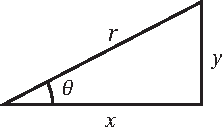
\includegraphics[]{math_primer/figures/trig.pdf}
    \caption{A right triangle.}
    \label{fig:triangle}
\end{figure}
The reciprocal of these relationships also have named functions (secant, $\sec$,
cosecant, $\csc$, and cotangent $\cot$), but are less often used,
\begin{align*}
    \sec \theta = \frac{1}{\cos \theta} & = \frac{r}{x} , \\
    \csc \theta = \frac{1}{\sin \theta} & = \frac{r}{y} , \\
    \cot \theta = \frac{1}{\tan \theta} & = \frac{x}{y} . \\
\end{align*}

We can define the inverse operation of these functions (e.g.\ $\cos^{-1} (\cos
\theta) = \theta$) as
\begin{align*}
    \theta & = \cos^{-1} \frac{x}{r} \\
    \theta & = \sin^{-1} \frac{y}{r} \\
    \theta & = \tan^{-1} \frac{y}{x}. \\
\end{align*}

\subsection{Law of Sines and Cosines}

A couple additional relationships that are useful from time to time are the law
of sines and law of cosines which define the relationships between the length of
the sides and the angles.
\begin{figure}[hbt]
    \centering
    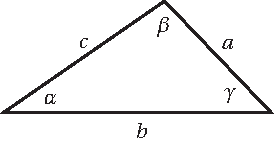
\includegraphics[]{math_primer/figures/trig2.pdf}
    \caption{Any triangle.}
    \label{fig:triangle}
\end{figure}

Law of Sines
\begin{equation*}
    \frac{\sin \alpha}{a} = \frac{\sin \beta}{b} = \frac{\sin \gamma}{c} .
\end{equation*}

Law of Cosines
\begin{equation}
    c^2 = a^2 + b^2 - 2ab \cos \gamma .
\end{equation}

\subsection{Trigonometry and the Unit Circle}

The trigonometric functions can be related to the equation of a circle by
\begin{equation}
    r^2 = \cos^{2} \theta + \sin^{2} \theta,
\end{equation}
where $\cos^{2} \theta = (\cos \theta)^2$ and the angle, $\theta$, measured
counterclockwise from the positive $x$-axis (Fig.~\ref{fig:unitcircle}).  A word
of caution should be given here about notation with respect to powers applied to
trigonometric functions because $\cos^{-1} z \neq (\cos z)^{-1}$ as you will see
below.
\begin{figure}[hbt]
    \centering
    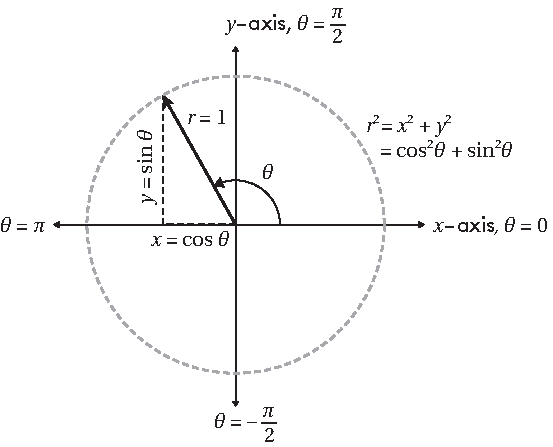
\includegraphics[]{math_primer/figures/unit_circle.pdf}
    \caption{The unit circle and its relationship to trigonometric functions.}
    \label{fig:unitcircle}
\end{figure}

Note: in geophysics, we typically define our angles in radians.  So unless
otherwise specified, assume radians.  There are $2\pi$ radians in a full circle.
Hence 0 is the same direction as $2\pi$, just as 0\deg\ is the same direction as
360\deg.  To convert from one to the other,
\begin{align*}
    \theta(\deg) &= \frac{180}{\pi} \theta(\mathrm{rad}), \\
    \theta(\mathrm{rad}) &= \frac{\pi}{180} \theta(\deg).
\end{align*}

\subsection{Trigonometric Identities}

There are a number of useful trigonometric identites than can be used
to simplify equations.  A selected set from \citet{Zwillinger1996} are included
below.

Pythagorean theorem
\begin{equation*}
    \sin^2 \theta + \cos^2 \theta = 1
\end{equation*}

Angle sum and difference relationships
\begin{align*}
    \sin(\alpha \pm \beta) &= \sin \alpha \cos \beta \pm \cos \alpha \sin \beta \\
    \cos(\alpha \pm \beta) &= \cos \alpha \cos \beta \mp \sin \alpha \sin \beta \\
    \tan(\alpha \pm \beta) &= \frac{\tan \alpha \pm \tan \beta}
        {1 \mp \tan \alpha \tan \beta} \\
    \sin \alpha \sin \beta &= \frac{1}{2} \cos (\alpha - \beta) 
        - \frac{1}{2} \cos (\alpha + \beta) \\
    \cos \alpha \cos \beta &= \frac{1}{2} \cos (\alpha - \beta) 
        + \frac{1}{2} \cos (\alpha + \beta) \\
    \sin \alpha \cos \beta &= \frac{1}{2} \sin (\alpha - \beta) 
        + \frac{1}{2} \sin (\alpha + \beta)
\end{align*}

Double and half angles
\begin{align*}
    \sin 2\theta &= 2\sin \theta \cos \theta 
        = \frac{2\tan \theta}{1 + 2 \tan^2 \theta} \\
    \cos 2\theta &= \cos^2 \theta - \sin^2 \theta 
        = 2\cos^2 \theta - 1 
        = 1 - 2 \sin^2 \theta
        = \frac{1 - \tan^2 \theta}{1 + \tan^2 \theta} \\
    \tan 2\theta &= \frac{2 \tan \theta}{1 - tan^2 \theta} \\
    \sin \frac{\theta}{2} &= \pm \left(\frac{1 - \cos \alpha}{2} \right)^{1/2} \\
    \cos \frac{\theta}{2} &= \pm \left(\frac{1 + \cos \alpha}{2} \right)^{1/2} \\
    \tan \frac{\theta}{2} &= \frac{1 + cos \theta}{\sin \theta}
        = \frac{\sin \theta}{1 - \cos \theta}
        = \pm \left( \frac{1 + \cos \theta}{1 - \cos \theta} \right)^{1/2}
\end{align*}
For half-angles the sign, $\pm$, depends upon quadrant.

Forward--inverse combinations
\begin{align*}
    \sin (\cos^{-1} x) &= (1 - x^2)^{1/2} \\
    \sin (\tan^{-1} x) &= x (1 + x^2)^{-1/2} \\
    \cos (\sin^{-1} x) &= (1 - x^2)^{1/2} \\
    \cos (\tan^{-1} x) &= (1 + x^2)^{-1/2} \\
    \tan (\sin^{-1} x) &= x (1 - x^2)^{-1/2} \\
    \tan (\cos^{-1} x) &= x^{-1} (1 - x^2)^{1/2} \\
\end{align*}

\bibliographystyle{elsarticle-harv}
\bibliography{ref}

\chapter{Complex Numbers: $i^2$ Keep it Real}

\section{The complex number: $i$} \label{apx:complex}
Electromagnetics makes heavy use of complex numbers, which we employ to tell us
about waves.  The representation of the complex quantity $i$ is defined as
\begin{equation}
    i \equiv \sqrt{-1}.
\end{equation}
This leads to the obvious result $i \cdot i = i^2 = -1$.

Perhaps you were taught in a previous math course that roots of negative numbers
was not allowed.  This is only true in that the root of a negative number cannot
produce a value along the real number line.  However, imagine a second number
line orthogonal (independent) of the real number line that does allow for roots
of complex values.  We call the set of numbers that fall along this line
imaginary numbers (Figure~\ref{fig:complex}).
\begin{figure}[hbt]
  \centerline{
    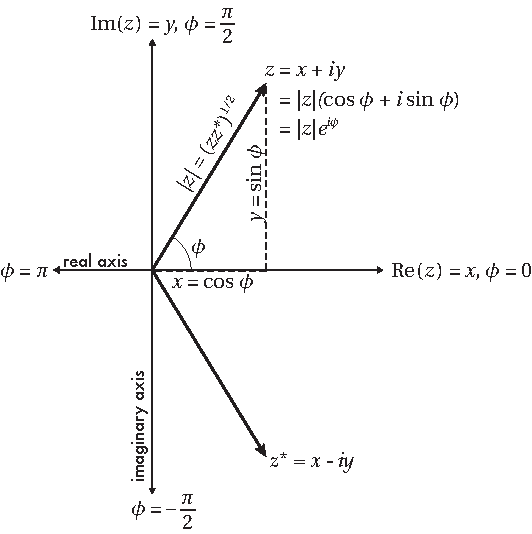
\includegraphics[]{math_primer/figures/complex_plane.eps}
  }
  \caption{Complex plane and relationships between orthogonal coordinates, 
  a circle, and the natural number.}
  \label{fig:complex}
\end{figure}

We can write a complex number $z$ as the combination of a {\it real},
$\Re$, and {\it imaginary}, $\Im$, parts,
\begin{equation*}
    z = a + i b, \\
\end{equation*}
where $a$ and $b$ are from the set of $\mathbb{R}$.  We can designate the real
part by $\Re (z)$ and the imaginary part by $\Im (z)$.  We will
define the complex conjugate ($*$) of a complex number as
\begin{equation}
    z^* = (a + i b)^* = a - i b.
\end{equation}
The norm (magnitude) of a complex number is a real number,
\begin{equation}
    \abs{z} \equiv (z z^*)^{1/2} \equiv (z^* z)^{1/2}
\end{equation}
Hence $\abs{z} = \left[(a + ib)(a - ib)\right]^{1/2} = \left[ a^2 + b^2
\right]^{1/2}$.  Note that the norm is also frequently written as $\norm{z}$ to
differentiate it somewhat from the absolute value; although, the absolute value
is the norm of a real number.  For a pure real number, $b = 0$, the norm is $a$;
for an pure imaginary number, $a = 0$, the norm is $b$.  Hence the real and
imaginary parts are orthogonal.

We can also write $z$ as
\begin{equation}
    z = \abs{z} \left( \frac{a}{\abs{z}} + i \frac{b}{\abs{z}} \right),
\end{equation}
where $-1 < a \abs{z}^{-1} < 1$ and $-1 < b \abs{z}^{-1} < 1$.  It can be shown
that in this form, we can relate the complex number to a circle allowing us to
write
\begin{equation}
    z = \abs{z} \left( \cos \theta + i \sin \theta \right), 
\end{equation}
where $\theta$ is an angle in radians. The angle $\theta$ represents the vector
angle associated with the magnitude and is defined by $\tan^{-1} \frac{b}{a}$.
We can also use the relation to show
\begin{equation}
    z = \abs{z} e^{i \theta},
\end{equation}
where $e$ is the natural number.  The above expression is a very useful one as
it allows us to write complex numbers in a very compact form.  It also yields
one of the most interesting relationships in mathematics, $e^{i \pi} = -1$.
\begin{figure}[hbt]
  \centerline{
    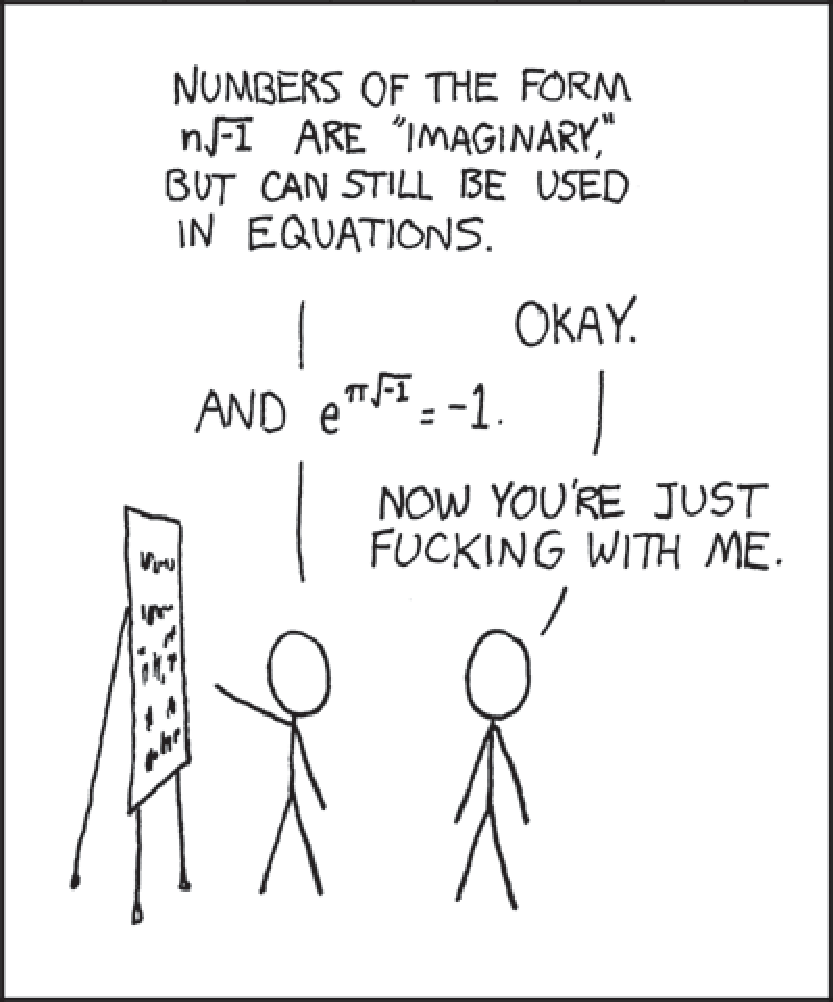
\includegraphics[width=15pc]{math_primer/figures/e_to_the_pi_times_i.eps}
  }
  \caption{$e$ to the $\pi$ times $i$.  Source: Randall Munroe,
  \protect\url{http://www.xkcd.org}.}
  \label{fig-eipi}
\end{figure}


\subsection{Algebra of Complex Numbers}

Complex numbers follow the usual algebraic rules, with the additional property
that $i^2 = -1$. For two complex numbers $z_1 = a + ib$ and $z_2 = c + id$,

\begin{align*}
    z_1 + z_2 &= (a+c) + i(b+d), \\
    z_1 z_2 &= (ac - bd) + i(ad + bc).
\end{align*}

Division is most easily performed by multiplying numerator and denominator by
the complex conjugate:
\begin{equation}
    \frac{z_1}{z_2} = \frac{z_1 z_2^*}{z_2 z_2^*}.
\end{equation}

In polar (exponential) form, multiplication and division become particularly
simple:
\begin{align}
    z_1 z_2 &= |z_1||z_2| e^{i(\theta_1 + \theta_2)}, \\
    \frac{z_1}{z_2} &= \frac{|z_1|}{|z_2|} e^{i(\theta_1 - \theta_2)}.
\end{align}


\subsection{Complex Representation of Oscillations}

Complex numbers provide a compact way to represent oscillatory behaviour. Using
Euler's identity,
\begin{equation}
    e^{i \omega t} = \cos(\omega t) + i \sin(\omega t),
\end{equation}
we can represent sinusoidal functions using complex exponentials.

In practice, we often work with expressions of the form
\begin{equation}
    z(t) = A e^{i(\omega t + \phi)},
\end{equation}
where $A$ is the amplitude, $\omega$ is angular frequency, and $\phi$ is the phase.

The physically observable quantity is typically the real part,
\begin{equation}
    \Re\left[ A e^{i(\omega t + \phi)} \right] = A \cos(\omega t + \phi).
\end{equation}

This representation greatly simplifies differentiation and integration:
\begin{align}
    \frac{d}{dt} e^{i \omega t} &= i \omega e^{i \omega t}, \\
    \int e^{i \omega t} \, dt &= \frac{1}{i\omega} e^{i \omega t}.
\end{align}


\section{Hyperbolic Functions}\label{apx:hyper}

Hyperbolic functions are closely related to trigonometric functions through
complex arguments:
\begin{align}
    \cosh z &= \cos(i z), \\
    \sinh z &= -i \sin(i z).
\end{align}

Hyperbolic functions commonly arise in problems involving exponential decay or
growth, such as diffusion and electromagnetic attenuation in conductive media.

For example, solutions of the form
\begin{equation}
    e^{-k z}
\end{equation}
can be written in terms of hyperbolic functions when boundary conditions are
applied.

As you have just seen, we have been able to relate trigonometric functions to
complex numbers.  It follows from the previous section then that we can write
the $\cos$, $\sin$, and $\tan$ as
\begin{align*}
    \cos z & = \frac{e^{i z} + e^{-i z}}{2} \\
    \sin z & = \frac{e^{i z} - e^{-i z}}{2i} \\
    \tan z & = \frac{e^{i z} - e^{-i z}}{e^{i z} + e^{-i z}}.
\end{align*}

We will now define a hyperbolic function in a very similar way as
\begin{align*}
    \cosh z & = \frac{e^{z} + e^{-z}}{2} \\
    \sinh z & = \frac{e^{z} - e^{-z}}{2} \\
    \tanh z = \frac{\sinh z}{\cosh z} & = \frac{e^{z} - e^{-z}}{e^{z} + e^{-z}},
\end{align*}
and their inverse functions as,
\begin{align*}
    \cosh^{-1} \left(\frac{e^{z} + e^{-z}}{2}\right) & = z \\
    \sinh^{-1} \left(\frac{e^{z} - e^{-z}}{2}\right) & = z \\
    \tanh^{-1} \left(\frac{e^{z} - e^{-z}}{e^{z} + e^{-z}}\right) & = z. \\
\end{align*}

\chapter{Linear Algebra: Stuck in the Matrix}

Up to this point we have written equations independent of each other.

Earlier we described our vectors by
\begin{equation}
    \vb{r} = (r_x,r_y,r_z) = r_x \vu{x} + r_y \vu{y} + r_z \vu{z} .
\end{equation}
However, there is another way.  We can express a vector as a either a single row
or single column matrix, e.g.
\begin{align}
    \mat{r} & = \begin{bmatrix}
            r_x & r_y & r_z
        \end{bmatrix} && \text{row vector} , \\
    & = \begin{bmatrix}
            r_x \\ r_y \\ r_z
        \end{bmatrix} && \text{column vector} . \\
\end{align}
Note: we change the notation for a vector from $\vb{r}$ to $\mat{r}$ when
we express it as a matrix.  While this change in notation is not really
necessary it is a commonly used convention.


\section{Matrix Math}

Matrix notation allows us to compactly represent systems of linear equations.
For example, a system of three equations in three unknowns can be written as
\begin{align}
    a_{11} x + a_{12} y + a_{13} z &= b_1 ,\\
    a_{21} x + a_{22} y + a_{23} z &= b_2 ,\\
    a_{31} x + a_{32} y + a_{33} z &= b_3 .
\end{align}
This can be expressed in matrix form as
\begin{equation}
    \mathbf{A} \vb{x} = \vb{b},
\end{equation}
where
\begin{equation}
    \mathbf{A} =
    \begin{bmatrix}
        a_{11} & a_{12} & a_{13} \\
        a_{21} & a_{22} & a_{23} \\
        a_{31} & a_{32} & a_{33}
    \end{bmatrix}, \quad
    \vb{x} =
    \begin{bmatrix}
        x \\ y \\ z
    \end{bmatrix}, \quad
    \vb{b} =
    \begin{bmatrix}
        b_1 \\ b_2 \\ b_3
    \end{bmatrix}.
\end{equation}

Matrix multiplication follows a row-by-column rule. The $(i,j)$ element of the
product $\mathbf{C} = \mathbf{A}\mathbf{B}$ is given by
\begin{equation}
    c_{ij} = \sum_{k} a_{ik} b_{kj}.
\end{equation}
This operation is only defined when the number of columns in $\mathbf{A}$ equals
the number of rows in $\mathbf{B}$.

Note that matrix multiplication is generally \emph{not commutative}, i.e.
\begin{equation}
    \mathbf{A}\mathbf{B} \neq \mathbf{B}\mathbf{A}.
\end{equation}


\section{Matrix Operators}

\subsection{Determinant}

The determinant is a scalar quantity associated with a square matrix. For a
$2\times2$ matrix,
\begin{equation}
    \mathbf{A} =
    \begin{bmatrix}
        a & b \\
        c & d
    \end{bmatrix},
\end{equation}
the determinant is
\begin{equation}
    \det(\mathbf{A}) = ad - bc.
\end{equation}

For a $3\times3$ matrix,
\begin{equation}
    \det(\mathbf{A}) =
    \begin{vmatrix}
        a_{11} & a_{12} & a_{13} \\
        a_{21} & a_{22} & a_{23} \\
        a_{31} & a_{32} & a_{33}
    \end{vmatrix},
\end{equation}
which can be expanded along the first row as
\begin{equation}
    \det(\mathbf{A}) =
    a_{11}
    \begin{vmatrix}
        a_{22} & a_{23} \\
        a_{32} & a_{33}
    \end{vmatrix}
    - a_{12}
    \begin{vmatrix}
        a_{21} & a_{23} \\
        a_{31} & a_{33}
    \end{vmatrix}
    + a_{13}
    \begin{vmatrix}
        a_{21} & a_{22} \\
        a_{31} & a_{32}
    \end{vmatrix}.
\end{equation}

The determinant has several important interpretations:
\begin{itemize}
    \item It measures the scaling of volume under the linear transformation.
    \item If $\det(\mathbf{A}) = 0$, the matrix is singular (non-invertible).
    \item The sign indicates orientation (e.g.\ right-handed vs left-handed).
\end{itemize}

\subsection{Transpose}

The transpose of a matrix, denoted $\mathbf{A}^T$, is obtained by swapping rows
and columns:
\begin{equation}
    (\mathbf{A}^T)_{ij} = a_{ji}.
\end{equation}

For example,
\begin{equation}
    \mathbf{A} =
    \begin{bmatrix}
        a_{11} & a_{12} \\
        a_{21} & a_{22}
    \end{bmatrix}
    \quad \Rightarrow \quad
    \mathbf{A}^T =
    \begin{bmatrix}
        a_{11} & a_{21} \\
        a_{12} & a_{22}
    \end{bmatrix}.
\end{equation}

Important properties include
\begin{align}
    (\mathbf{A}^T)^T &= \mathbf{A}, \\
    (\mathbf{A}\mathbf{B})^T &= \mathbf{B}^T \mathbf{A}^T.
\end{align}

A matrix is called \emph{symmetric} if $\mathbf{A}^T = \mathbf{A}$.

\subsection{Inverse}

The inverse of a matrix $\mathbf{A}$, denoted $\mathbf{A}^{-1}$, satisfies
\begin{equation}
    \mathbf{A}^{-1} \mathbf{A} = \mathbf{A} \mathbf{A}^{-1} = \mathbf{I},
\end{equation}
where $\mathbf{I}$ is the identity matrix.

For a $2\times2$ matrix,
\begin{equation}
    \mathbf{A} =
    \begin{bmatrix}
        a & b \\
        c & d
    \end{bmatrix},
\end{equation}
the inverse is
\begin{equation}
    \mathbf{A}^{-1}
    =
    \frac{1}{ad - bc}
    \begin{bmatrix}
        d & -b \\
        -c & a
    \end{bmatrix},
\end{equation}
provided that $\det(\mathbf{A}) \neq 0$.

For larger matrices, the inverse is typically computed using row reduction or
numerical methods.

In practice (especially in geophysics), it is often preferable to solve
\begin{equation}
    \mathbf{A}\vb{x} = \vb{b}
\end{equation}
without explicitly computing $\mathbf{A}^{-1}$, as direct inversion can be
numerically unstable and computationally expensive.

\section{Eigenvalues and Eigenvectors}

Eigenvalues and eigenvectors describe how a matrix transforms a vector. In
particular, they identify directions that are stretched or compressed without
being rotated.

An eigenvector $\vb{v}$ of a matrix $\mathbf{A}$ satisfies
\begin{equation}
    \mathbf{A} \vb{v} = \lambda \vb{v},
\end{equation}
where $\lambda$ is the corresponding eigenvalue.

This equation says that applying $\mathbf{A}$ to $\vb{v}$ simply scales the
vector by a factor $\lambda$, without changing its direction.

To compute eigenvalues, we rewrite the equation as
\begin{equation}
    (\mathbf{A} - \lambda \mathbf{I}) \vb{v} = \vb{0}.
\end{equation}
For non-trivial solutions ($\vb{v} \neq \vb{0}$), we require
\begin{equation}
    \det(\mathbf{A} - \lambda \mathbf{I}) = 0.
\end{equation}
This is called the \emph{characteristic equation}, and its solutions give the
eigenvalues $\lambda$.

Once the eigenvalues are known, the corresponding eigenvectors are found by
solving
\begin{equation}
    (\mathbf{A} - \lambda \mathbf{I}) \vb{v} = \vb{0}.
\end{equation}

Eigenvalues and eigenvectors have important physical interpretations. In
geophysics, for example:
\begin{itemize}
    \item Eigenvectors often represent principal directions (e.g.\ principal
    stress or strain axes).
    \item Eigenvalues represent magnitudes along those directions.
\end{itemize}

For symmetric matrices, which commonly arise in physical problems, eigenvectors
are orthogonal and eigenvalues are real. This greatly simplifies their
interpretation.

\section{Singular Value Decomposition (SVD)}

The singular value decomposition (SVD) is one of the most powerful and widely
used tools in linear algebra, particularly for solving inverse problems and
analyzing ill-conditioned systems.

Any $m \times n$ matrix $\mathbf{A}$ can be written as
\begin{equation}
    \mathbf{A} = \mathbf{U} \boldsymbol{\Sigma} \mathbf{V}^T,
\end{equation}
where
\begin{itemize}
    \item $\mathbf{U}$ is an $m \times m$ orthogonal matrix,
    \item $\mathbf{V}$ is an $n \times n$ orthogonal matrix,
    \item $\boldsymbol{\Sigma}$ is an $m \times n$ diagonal matrix containing
    non-negative values.
\end{itemize}

The diagonal entries of $\boldsymbol{\Sigma}$,
\begin{equation}
    \sigma_1 \geq \sigma_2 \geq \cdots \geq 0,
\end{equation}
are called the \emph{singular values} of $\mathbf{A}$.

\subsection*{Interpretation}

The SVD provides a geometric interpretation of a matrix as a sequence of three
operations:
\begin{enumerate}
    \item $\mathbf{V}^T$: rotates the input vector into a new coordinate system,
    \item $\boldsymbol{\Sigma}$: stretches (or compresses) along orthogonal
    directions,
    \item $\mathbf{U}$: rotates the result into the final coordinate system.
\end{enumerate}

Thus, $\mathbf{A}$ maps a unit sphere into an ellipsoid, whose principal axes
are given by the columns of $\mathbf{U}$ and whose lengths are the singular
values $\sigma_i$.

\subsection*{Connection to Eigenvalues}

The singular values are related to the eigenvalues of $\mathbf{A}^T \mathbf{A}$:
\begin{equation}
    \mathbf{A}^T \mathbf{A} \vb{v}_i = \sigma_i^2 \vb{v}_i,
\end{equation}
where $\vb{v}_i$ are the columns of $\mathbf{V}$. Similarly,
\begin{equation}
    \mathbf{A} \mathbf{A}^T \vb{u}_i = \sigma_i^2 \vb{u}_i,
\end{equation}
where $\vb{u}_i$ are the columns of $\mathbf{U}$.

\subsection*{Rank and Singular Values}

The rank of $\mathbf{A}$ is equal to the number of non-zero singular values:
\begin{equation}
    \mathrm{rank}(\mathbf{A}) = \# \{ \sigma_i > 0 \}.
\end{equation}

Small singular values indicate directions in which the matrix has little
sensitivity. In practice, very small $\sigma_i$ are often treated as zero,
revealing effective rank deficiency.

\subsection*{Solving Linear Systems}

The SVD provides a stable way to solve
\begin{equation}
    \mathbf{A} \vb{x} = \vb{b},
\end{equation}
especially when $\mathbf{A}$ is ill-conditioned or not square.

The solution can be written as
\begin{equation}
    \vb{x} = \mathbf{V} \boldsymbol{\Sigma}^{-1} \mathbf{U}^T \vb{b},
\end{equation}
where $\boldsymbol{\Sigma}^{-1}$ is formed by inverting the non-zero singular
values.

If some singular values are zero (or very small), the inverse does not exist in
the usual sense. In this case, we use the \emph{pseudo-inverse},
\begin{equation}
    \mathbf{A}^{+} = \mathbf{V} \boldsymbol{\Sigma}^{+} \mathbf{U}^T,
\end{equation}
which provides the least-squares solution.

\subsection*{Importance in Geophysics}

SVD is particularly useful in geophysical applications:
\begin{itemize}
    \item It reveals rank deficiency and non-uniqueness in inverse problems.
    \item It identifies poorly constrained model parameters (small $\sigma_i$).
    \item It provides a natural framework for regularization by damping small
    singular values.
\end{itemize}

For these reasons, SVD is a central tool in modern inversion theory.

\section{Matrix Rank}

The \emph{rank} of a matrix is the number of linearly independent rows or
columns in the matrix. It provides a measure of how much independent
information the matrix contains.

For a matrix $\mathbf{A}$,
\begin{equation}
    \mathrm{rank}(\mathbf{A}) = \text{number of linearly independent rows}
    = \text{number of linearly independent columns}.
\end{equation}

Some important consequences:
\begin{itemize}
    \item If $\mathbf{A}$ is an $n \times n$ matrix and
    $\mathrm{rank}(\mathbf{A}) = n$, then $\mathbf{A}$ is full rank and
    invertible.
    \item If $\mathrm{rank}(\mathbf{A}) < n$, then $\mathbf{A}$ is singular and
    does not have an inverse.
    \item The rank determines the number of independent equations in a system
    $\mathbf{A}\vb{x} = \vb{b}$.
\end{itemize}

Geometrically, the rank tells us the dimension of the space spanned by the
matrix columns:
\begin{itemize}
    \item Rank 1: all columns lie along a line.
    \item Rank 2: columns span a plane.
    \item Rank 3: columns span a volume (in $\mathbb{R}^3$).
\end{itemize}

In practice, rank is determined by performing row reduction to bring the matrix
into row echelon form. The number of non-zero rows (or pivots) is the rank.

Rank is particularly important in geophysical inversion problems:
\begin{itemize}
    \item A rank-deficient system indicates redundancy or insufficient data.
    \item It may lead to non-unique solutions.
    \item Regularization methods are often used to handle such cases.
\end{itemize}
\chapter{Vectors: How far and which direction to the nearest pub?}
\epigraph{ ``[The vector] has never been of the slightest use to any creature.''}
{{\normalfont ---\ Lord Kelvin}}

\label{apx:vectors}

\section{Magnitude and Direction}
If I were to ask you, ``How hot is it today?'' You would respond with a single
number for the temperature.  If I were to ask, ``Where is the nearest pub?'' You
would likely tell me both how far and what direction to walk.

Why would you respond to the former question with one value while giving two
values for the latter?

Some physical quantities such as temperature, mass, charge, and energy require
one value in space and time to completely describe them.  Others such as
velocity, gravitational acceleration, electric field strength, and heat flow are
directional and require both a magnitude and direction to fully describe them.
So lets explore the world of vectors as we will encounter many in the course of
study.

Returning to the question of the nearest pub, you might tell me that there is
one three blocks south and four blocks west.  You gave me both a direction to
walk and a distance to travel.  But you did more than that.  Since the streets
of Adelaide proper are laid out on a north--south and east-west grid you
provided be with directions I would have to walk to get there (the
components).  So we can write down my position vector relative to the
pub mathematically as
\begin{equation}
    \vb{r} = (r_x,r_y) ,
\end{equation}
where $\vb{r}$ is the position vector and $r_x$ and $r_y$ are my distances north
and east of the pub.  The For the sake of simplicity we need to make a couple
assumptions:
\begin{itemize}
    \item the distance of a north-south block is the same as the distance of an
    east-west block (i.e. unit distances in the $x$, and $y$ directions are
    equivalent length); and
    \item north-south and east-west blocks are at right angles (i.e. the axes
    are {\it orthogonal} to each other).
\end{itemize}
These assumptions will simplify the math and are standard for any Cartesian
reference frame.  However, axes need not be orthogonal as we see for hexagonal
and triclinic mineral systems but we won't use these in the course.
\begin{figure}[hbt]
    \centering
    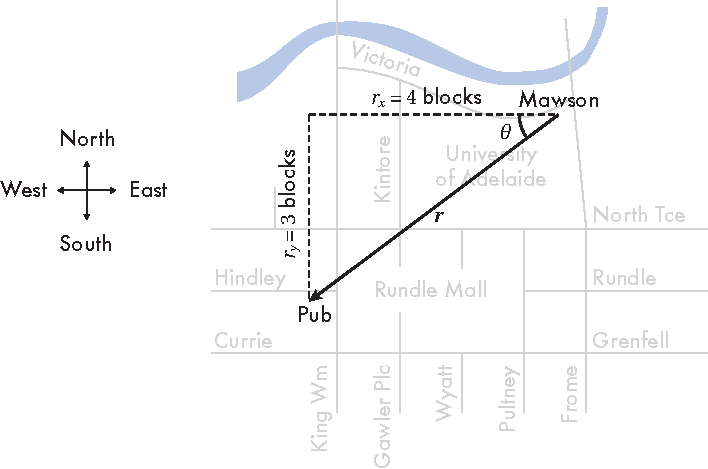
\includegraphics[]{math_primer/figures/position_vector.pdf}
    \caption{Position vector from Mawson Labs to a nearby pub.}
    \label{fig:posvec}
\end{figure}

\ntextbox{Notation}{
    When discussing vectors we use a bold letter, e.g, $\vb{r}$.  Since it is difficult to bold characters on a chalkboard or paper there are some common notations for vectors: $\vec{r}$ or $\utilde{r}$.  Likewise, there are multiple ways to write the components of a vector.  The components are frequently written with a subscript indicating the direction to which they refer, e.g. $r_x$.  As above, we can represent a vector as $\vb{r} = (r_x,r_y)$.  We can also write a vector in terms of it's components as
    \[
        \vb{r} = r_x \vu{x} + r_y \vu{y} ,
    \]
    where $\vu{x}$ and $\vu{y}$ are unit vectors, vectors of unit length in the direction of the labeled axis.  Because the direction of the unit vectors are orthogonal they cannot be added to produce a single quantity.
}{alert}

The directions to the pub are the vector components, but what I am interested in are the distance and direction from Mawson Labs.  We need a way to compute the distance from the components.  But we cannot simply add the length of $r_x$ and the length of $r_y$ because they are in mutually exclusive directions.  As you can see in Figure~\ref{fig:posvec} the individual components form the legs of a right triangle with the hypotenuse defined as the position vector.  So all we have to do is remember the Pythagorean theorem.  We can then write the magnitude/length/norm of the position vector as
\begin{equation}
    \norm{\vb{r}} = r = (r_x^2 + r_y^2)^{1/2} ,
\end{equation}
where $\norm{r}$ is called the norm.  Since we are lazy, we typically just write the magnitude as a roman, rather than bold, $r$.  Note: the norm is always positive.

The direction is determined by the signed ratio of the components
\begin{equation}
    \theta = \tan^{-1} \left( \frac{r_y}{r_x} \right),
\end{equation}
where $\tan^{-1}$ is the inverse of the tangent function.  Since the tangent
function has a $90\deg$ ambiguity, defined from $[-\pi/2,\pi/2]$ radians, we
must keep track of the sign on the $x$-component and add an additional $\pi$
radians if $r_x$ is negative.

We can extend our definitions to 3-dimensional space (suppose I had to go down
some stairs to get to the pub) by
\begin{equation}
    \norm{\vb{r}} = (r_x^2 + r_y^2 + r_z^2)^{1/2} .
\end{equation}
The direction is a bit trickier in this case since I now need two angles to
describe the orientation of my position vector.  We can define one angle as
before, but the second is defined as
\begin{equation}
    \phi = \cos^{-1} \left( \frac{r_z}{r} \right).
\end{equation}


\section{Changing of coordinate systems}
We will now consider several properties of a vector before turning to the rules .

\section{Addition and subtraction}

Adding vectors is very simple.  Graphically, we can add vectors by placing the
tail of one on the head of another (Figure~\ref{fig:sumdiff}.  The resultant
vector is determined simply by separately summing the individual components,
\begin{equation}
    \vb{a} + \vb{b} = (a_x + b_x)\vu{x} 
    + (a_y + b_y)\vu{y} + (a_z + b_z)\vu{z} .
\end{equation}
\begin{figure}[hbt]
    \centering
    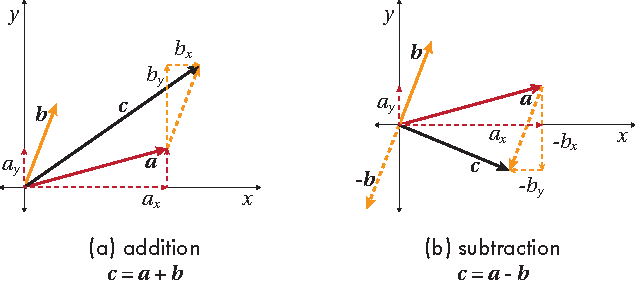
\includegraphics[]{math_primer/figures/vectors_sumdiff.pdf}
    \caption{Vector addition (a) and subtraction (b) in two dimensions.}
    \label{fig:sumdiff}
\end{figure}

Subtraction of vectors is very similar to the addition, again minding the
individual components,
\begin{equation}
    \vb{a} - \vb{b} = (a_x - b_x)\vu{x} 
    + (a_y - b_y)\vu{y} + (a_z - b_z)\vu{z} .
\end{equation}

Rules for addition and subtraction of vectors are very similar to the rules for
scalars,
\begin{align}
    \vb{a} + \vb{b} &= \vb{b} + \vb{c} && \text{commutative} \\
    \vb{a} + (\vb{b} + \vb{c}) &= (\vb{a} + \vb{b}) + \vb{c} && \text{associative} \\
    \vb{a} - (\vb{b} - \vb{c}) &= (\vb{a} - \vb{b}) - \vb{c} && \text{associative} \\
\end{align}

\section{Multiplication of vectors}
Multiplication of vectors is not difficult but there are some differences from
traditional scalar multiplication.  For starters, there are two types of vector
multiplication: the scalar (or inner, or dot) product and the cross (or outer)
product.

\subsection{Scalar (inner) product}

In scalar multiplication the length of the original number $a$ is extended $b$
times.  Scalar multiplication is very similar in this respect as the length of
the individual vector components of $\vb{a}$ are extended by the length of the
individual components of $\vb{b}$ times.  We use $\cdot$ (dot) to represent
operator scalar product operator.  The scalar product of two vectors is given by
\begin{equation}
    \vb{a}\cdot\vb{b} = a_x b_x + a_y b_y + a_z b_z .
\end{equation}
Note: the scalar product of two vectors results in a scalar.  This property is
very useful since we generally much prefer to work with scalars over the
multiple components of a vector.

\begin{equation}
    \vb{a} \cdot \vb{b} = ab \cos \theta .
\end{equation}
Recall that $a$ and $b$ are the shortened representation for the lengths (norms)
of the vectors $\vb{a}$ and $\vb{b}$, respectively.


The norm that we discussed earlier is related to the dot product by
\begin{equation}
    \norm{\vb{r}} = (\vb{r}\cdot\vb{r})^{1/2} = (r_x^2 + r_y^2 + r_z^2)^{1/2} .
\end{equation}

\subsection{Cross (outer) product}
The cross product of a vector is
\begin{equation}
    \vb{a} \times \vb{b} = (a_y b_z - a_z b_y) \vu{x} 
    + (a_z b_x - a_x b_z) \vu{y} + (a_x b_y - a_y b_x) \vu{z}
\end{equation}


\section{Derivative of a vector}
Up to this point we have discussed the derivative of a scalar function
(speed).  The meaning of speed is familiar and you may have heard the term
velocity used to mean much the same thing.  But in physics there is a 
difference between speed and velocity.  Speed refers to a rate of travel, but
velocity refers to direction as well as speed.  We make this distinction because
many things in nature depend on the direction of two things relative to each
other.

Let's return to the example of my bike ride into work.  We previously discussed
my path as if it was straight (one-dimensional) but my position in space wasn't
really constrained to one dimension (linear park is not a straight path).  On my
ride, I take numerous gentle turns to the right and left and even up and down.
Hence my path was three-dimensional, but we'll assume it was just two
dimensional to illustrate what makes the vector velocity different than speed.

\chapter{Coordinate Systems}
What is a coordinate system?  We use a coordinate system to specify positions
relative to each other.  We live in a four-dimensional space, three which are
true spatial dimensions and the fourth is time.  Time is simple, as we will call
it $t$. For the other three dimensions, we will describe each discrete point in
space as a combination of coordinates relative to a defined point (origin).

Why do we need more than one coordinate system?  Our choice of coordinate system
can be used to simplify the math and explore symmetries of bodies with ideal
geometries.  We will only use the three listed below (Figure~\ref{fig:coords}),
although there are many others (think of the plethora of map projections
available).
\begin{figure}[hbt]
  \centerline{
    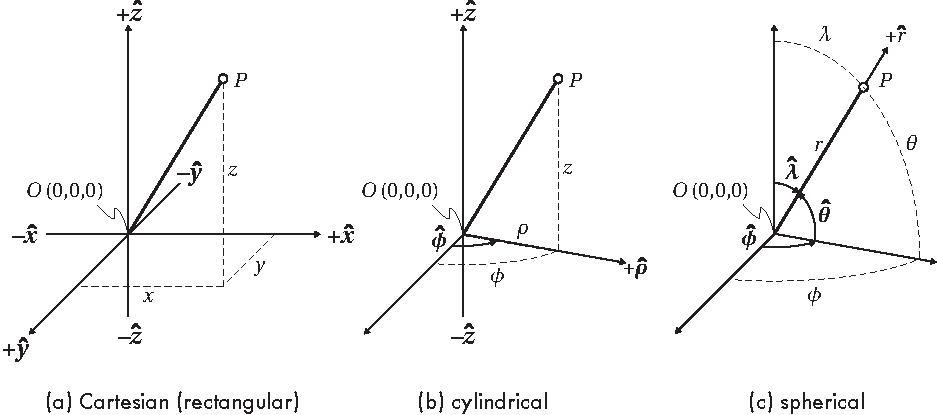
\includegraphics[]{math_primer/figures/coordinate_systems.pdf}
  }
  \caption{Commonly used coordinate systems. Axes labels with a $\hat{\ }$
  indicate a unit vector (vector of unit length).}
  \label{fig:coords}
\end{figure}

\section{Cartesian}
The first coordinate system to consider (and most familiar) is a {\it Cartesian
(rectangular) coordinate system} (Figure~\ref{fig:coords}a).  To describe our
space we will typically use the variables $x$, $y$, and $z$ and as a result each
point in space is defined by the coordinate triplet $(x,y,z)$.  In a Cartesian
system the principle axes (directions) are each orthogonal (at right angles) to
each other.

We will define our coordinate system such that it is right-handed.  To get an
intuitive feeling for what this means, take your right hand open with fingers
extended.  The direction your fingers point is the positive $x$-direction.  Now
keeping your fingers straight, bend your knuckles that join the fingers to the
palm.  Your palm and fingers should now form a right angle.  This is the
positive $y$-axis.  To determine the positive $z$-direction point your thumb out
away from your hand.  In geophysics we frequently choose the most convenient
coordinate system for our direction of interest.  If we are looking down into
the Earth for instance, we typically define the positive $z$-axis as down,
implying the cardinal directions $north$ and $east$ are the positive $x$- and
positive $y$-axes, respectively.  This definition of $+z$ down occasionally
reverses the sign of equations derived in physics, which has the amusing
side-effect of occasionally confuses physicists.  For short, we can identify
this coordinate system as NED, (north, east, down) = $(+x, +y, +z)$.

\section{Polar}
The polar coordinate system is a two-dimensional coordinate system that is
special case of cylindrical and spherical coordinates when $z = 0$ or $\theta =
0$, respectively.

Conversion from Cartesian $\leftrightarrow$\ polar:
\begin{align*}
    r &= (x^2 + y^2)^{1/2} & x &= r \cos \phi \\
    \phi &= \tan^{-1} \frac{y}{x} & y &= r \sin \phi \\
    \vu{r} &= \cos \phi \,\vu{x} + \sin \phi \,\vu{y} &
    \,\vu{x} &= \cos \phi \,\vu{r} - \sin \phi \,\vu{\phi} \\
    \vu{\phi} &= -\sin \phi \,\vu{x} + \cos \phi \,\vu{y} &
    \,\vu{y} &= \sin \phi \,\vu{r} + \cos \phi \,\vu{\phi} \\
\end{align*}

\section{Cylindrical}
We may also define a {\it cylindrical coordinate system} which we define as $\rho$, $\phi$, and $z$ (Figure~\ref{fig:coords}b).  Imagine a circular cylinder with the $z$-direction forming the axis of the cylinder.  The cross-section of the cylinder defines a circle with radius $\rho$.  The third coordinate is an angle $\phi$ defined clockwise in the plane of the cylinder's cross section.  Systems which are cylindrically symmetric are called axially symmetric and variations are typically described in terms of the axial ($z$) direction and radial direction (cross-section of the cylinder).  Note: because the radius is defined differently for the cylindrical and spherical coordinate systems, we use $\rho$ for the radius in cylindrical coordinates to differentiate it from $r$ used in spherical coordinates.

Conversion from Cartesian $\leftrightarrow$\ cylindrical:
\begin{align*}
    \rho &= (x^2 + y^2)^{1/2} & x &= \rho \cos \phi \\
    \phi &= \tan^{-1} \frac{y}{x} & y &= \rho \sin \phi \\
    z &= z & z &= z \\
    \vu{r} &= \cos \phi \,\vu{x} + \sin \phi \,\vu{y} &
    \vu{x} &= \cos \phi \,\vu{r} - \sin \phi \,\vu{\phi} \\
    \vu{\phi} &= -\sin \phi \,\vu{x} + \cos \phi \,\vu{y} &
    \vu{y} &= \sin \phi \,\vu{r} + \cos \phi \,\vu{\phi} \\
    \vu{z} &= \,\vu{z} & \,\vu{z} &= \,\vu{z}
\end{align*}

\section{Spherical}
A third coordinate system commonly used in geophysics is a {\it spherical
coordinate system} (Figure~\ref{fig:coords}c). Points within this system are
defined by the radius of a sphere $r$ and two angles that describe where $r$
points.  One angle about the equator (longitude), $\phi$, defined counter
clockwise and the second is defined from the north pole to south pole
(co-latitude), $\theta$.  For many Earth applications, we use the latitude as an
angle defined from the equator to the pole, $\lambda$, where the latitude is
related to the co-latitude by $\lambda = 90 - \theta$ in degrees.  Systems which
are spherically symmetric are described in terms of a radial direction only.

Conversion from Cartesian $\leftrightarrow$ spherical:
\begin{align*}
    r &= (x^2 + y^2 + z^2)^{1/2} & x &= r \sin \theta \cos \phi \\
    \theta &= \cos^{-1} \frac{z}{r} & y &= r \sin \theta \sin \phi \\
    \phi &= \tan^{-1} \frac{y}{x} & z &= r \cos \theta \\
    \vu{r} &= \sin \theta \cos \phi \,\vu{x} + \sin \theta \sin \phi
        \,\vu{y} + \cos \theta \,\vu{z} &
    \vu{x} &= \sin \theta \cos \phi \,\vu{r} + \cos \theta \cos \phi
        \,\vu{\theta} - \sin \phi \,\vu{\phi} \\
    \vu{\theta} &= \cos \theta \cos \phi \,\vu{x} + \cos \theta \sin \phi
        \,\vu{y} - \sin \theta \,\vu{z} &
    \vu{y} &= \sin \theta \sin \phi \,\vu{r} + \cos \theta \sin \phi
        \,\vu{\theta} + \cos \phi \,\vu{\phi} \\
    \vu{\phi} &= \sin \phi \,\vu{x} + \cos \phi \,\vu{y} &
    \vu{z} &= \cos \theta \,\vu{r} - \sin \theta \,\vu{\theta}
\end{align*}

Conversion from cylindrical $\leftrightarrow$ spherical:
\begin{align*}
    r &= (\rho^2 + z^2)^{1/2} & x &= r \cos \phi \\
    \theta &= \tan^{-1} \frac{\rho}{z} = \cos^{-1} \frac{z}{r} &
        y &= r \sin \phi \\
    \phi &= \phi & z &= z \\
    \vu{r} &= \sin \theta \,\vu{\rho} + \cos \theta \,\vu{z} &
    \vu{\rho} &= \sin \theta \,\vu{r} + \cos \theta \,\vu{\theta} \\
    \vu{\theta} &= \cos \theta \,\vu{\rho} - \sin \theta \,\vu{z} &
    \vu{z} &= \cos \theta \,\vu{r} - \sin \theta \,\vu{\theta} \\
    \vu{\phi} & = \,\vu{\phi} & \,\vu{\phi} &= \,\vu{\phi}
\end{align*}

\section{Derivatives}

\section{Integrals}
Suppose we wanted to take an integral along a path or about an area or volume but we wish to change coordinate systems to simplify the math.  In this case we have to change the infintesimal.  In the case of a line integral,
\begin{equation*}
    \dd{\ell} = 
    \begin{cases}
        \vu{x} \dd{x} + \vu{y} \dd{y} + \vu{z} \dd{z} & \text{Cartesian} \\
        \vu{\rho} \dd{\rho} + \vu{\phi} \rho \dd{\phi} + \vu{z} \dd{z} &
            \text{cylindrical} \\
        \vu{r} \dd{r} + \vu{\theta} r \dd{\theta} + \vu{\phi} r \sin
            \theta \dd{\phi} & \text{spherical}\\
    \end{cases}
\end{equation*}
Integrals over area do not have a simple conversion in the same way because it
depends on the direction of the point to the origin.

For a volume integral,
\begin{equation*}
    \dd{v} =
    \begin{cases}
        \dd{x} \dd{y} \dd{z} & \text{Cartesian} \\
        \rho \dd{\rho} \dd{\phi} \dd{z} & \text{cylindrical} \\
        r^2 \sin \theta \dd{r} \dd{\theta} \dd{\phi} & \text{spherical} \\
    \end{cases}
\end{equation*}

\chapter{Calculus: There's Sum Difference}\label{apx:calculus}

Calculus is one of the most useful set of mathematical techniques that a
geophysicist employs in their toolkit.  While some physics derivations can be
done with algebra, they are often far simpler to express and perform in terms of
calculus.  While many students place a mental barrier at the mere mention of
calculus, many of the concepts are really quite simple.

\section{Derivatives: How fast am I going?} \label{apx:derivatives}

\subsection{Rates of change}
Something you are undoubtably familiar with is traveling.  Traveling from home
to school in a car, on a bus, by foot?  In my case I biked to uni this morning.
I started at home (let's call it point $H$) at $t_0$ and arrived at the uni
(point $U$) some time later, $t_1$, for a total travel time $\Delta t = t_1 -
t_0$.  The distance traveled as the crow flies---there are no crows here... as
the magpie(?) flies---going from $H$ to $U$ is $\Delta x = x_1 - x_0$.

\vspace{8pt}
\noindent {\it How fast was I travelling?}

We can write my speed as
\begin{align*}
    \mathrm{speed} = & \frac{\mathrm{distance travelled}}{\mathrm{time elapsed}} \\
    v = & \frac{\Delta x}{\Delta t} .
\end{align*}
Graphically this represents the {\it slope} of a line on our graph
(Figure~\ref{fig:vavg1}).
\begin{figure}[hbt]
    \centering
    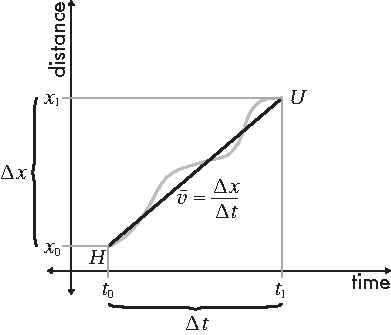
\includegraphics[]{math_primer/figures/average_velocity.pdf}
    \caption{Average velocity on the bike ride beween home and work.}
    \label{fig:vavg1}
\end{figure}

But of course I didn't travel at a constant rate.  The speed we just expressed
was the average speed,
\begin{equation*}
    \bar{v} = \frac{\Delta x}{\Delta t} .
\end{equation*}
So lets redraw the time-distance curve to something more realistic
(Figure~\ref{fig:vavg2}).
\begin{figure}[hbt]
    \centering
    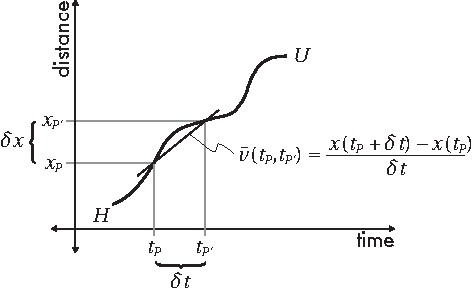
\includegraphics[]{math_primer/figures/average_velocity2.pdf}
    \caption{Average velocity during a short interval of time.}
    \label{fig:vavg2}
\end{figure}

\vspace{8pt}
\noindent {\it What was my speed as a function of time, i.e. v(t)?}

To derive this let's look first at how fast was I traveling at a single point,
$P$.  As we shown above, the speed is the slope of a line.  But we have a curve.
So lets take another point, $P'$, some time after $P$.  I passed $x_P$ at $t_P$
and $x_{P'}$ at $t_{P'}$.  We can compute the {\it average} speed between these
two points in time as
\begin{equation*}
    \bar{v}(t_P,t_{P'}) = \frac{x_{P'} - x_P}{t_{P'} - t_P} 
        = \frac{\delta x}{\delta t}.
\end{equation*}
But as before let's call the interval in time $\delta t$, which is $\delta t =
t_P - t_{P'}$.  And since $x$ is a function of time, $x = x(t)$.  So lets
rewrite the previous equation
\begin{equation*}
    \bar{v}(t_P,t_{P'}) = \frac{x(t_P + \delta t) - x(t_P)}{\delta t} .
\end{equation*}
``Ah,'' you say, ``but this is still an average velocity, we still don't know
the velocity at P.''  So what if we move the point $P'$ closer to $P$ and closer
still and then even closer until the two points $P$ and $P'$ are almost
coincident, i.e. $\delta t$ approaches 0 (Figure~\ref{fig:vinst}).
\begin{figure}[hbt]
    \centering
    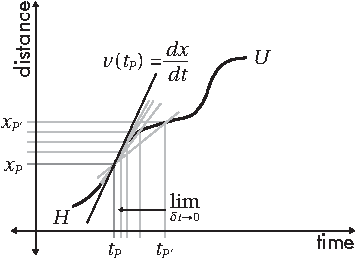
\includegraphics[]{math_primer/figures/instantaneous_velocity.pdf}
    \caption{Approximation of the instantaneous velocity by computing the
    average over smaller and smaller time intervals.}
    \label{fig:vinst}
\end{figure}
It is still an average, but the average will---assuming the function is {\it
continuous} and well-behaved---become a more accurate estimate of the {\it
instantaneous} speed at $t_P$.  We call the process of moving $P'$ towards $P$
as a {\it limit}, which we write as
\begin{equation*}
    \lim_{\delta t \to 0} \frac{x(t_P + \delta t_P) - x(t_P)}{\delta t} ,
\end{equation*}
In words we would say the ``in the limit $\delta t$ approaches 0...''  If our
assumptions hold true, then we are computing the average speed on a time
interval so small that it is effectively equal to the instantaneous speed at
$t_P$.  So we will now write this result not as the average but as the
instantaneous speed,
\begin{equation*}
    v(t_P) = \lim_{\delta t \to 0} \frac{x(t_P + \delta t_P) - x(t_P)}{\delta t} .
\end{equation*}
The above statement is the definition of the derivative which we write as
\begin{equation*}
    v(t_P) = \left. \dv{x}{t} \right|_{t = t_P} .
\end{equation*}
To indicate that the derivative represents the instantaneous change, we change
the $\delta$ to a $d$.  We cannot cancel the $d$'s as they are symbols denoting
the operation of a derivative in this case, not The vertical bar tells us that
we are evaluating our derivative at the point in time $t_P$.  But we didn't just
write a way to find my instantaneous speed at $P$, we now have a way to
determine my instantaneous speed at any point in time on my trip from home to
uni---assuming my journey was continuous and {\it differentiable} everywhere
along the path.  We can write the instantaneous speed as the derivative of
position with respect to time:
\begin{equation*}
    v(t) = \dv{}{t} x(t) = \dv{x}{t}.
\end{equation*}

What this tells us is that if we want to know my instantaneous speed at any
point in time, we simply take the derivative of position with respect to time
and evaluate at our point of interest.  It also means that the derivative of a
function is equal to the slope of---and is tangent to---the function at every
point along its path.

I used the word differentiable earlier as an assumption to write down the
more general mathematical statement.  So what determines if something is
differentiable.  For something to be differentiable, the limit must simply
exist.  But in our case we also want the function to be continuous which means
that there are no breaks (jumps), holes in the graph (a point that cannot
exist), or kinks (radical changes in slope at a point).  So in this case, the
limit must exist whether we approach our point from one side or the other (e.g.,
$\lim_{t \to t_P^-} = \lim_{t \to t_P^+}$).

Thus far, we have assumed by trip beween home and work is in 1-dimension.
Obviously this assumption over-simplifies the problem since my cycle trip to
work took numerous turns left and right, and up- and downhill.  For the time
being we will leave the one-dimensional case and we will return to the
multi-dimensional case after discussing vectors (Tutorial~\ref{apx:vectors}).


\subsection{Derivative definition}
The derivative represents the slope of a function.  So consider a function
$F(x)$ that is smooth and continuous (i.e.\ there are no jumps or changes in
slope at a point).  Recall that the slope between two points on a line is the
difference in magnitude evaluated at each point divided by the distance between
the points (Figure~\ref{fig:dx}).  For our two points on an arbitrary function,
we will choose our points at $x_{0}$ and $x_{0} + \delta\! x$ where $\delta\! x$
is a small positive value.  Assuming the slope is linear between these points,
we can write the slope
\begin{align*}
    m & \approx \frac{F(x_{0} + \delta\! x) - F(x_{0})}{(x_{0} + \delta\! x) - x_{0}} \\
      & \approx \frac{F(x_{0} + \delta\! x) - F(x_{0})}{\delta\! x}.
\end{align*}
A derivative is defined in the case where $\delta\! x$ approaches zero,
\begin{equation}
    \dv{F(x)}{x} \equiv 
        \lim_{\delta\! x \to 0} \frac{F(x_{0} + \delta\! x) - F(x_{0})}{\delta\!  x},
    \label{eq:derivative}
\end{equation}
where $\dd{F(x)}/\dd{x}$ is the standard notation for a derivative and
$\lim_{\delta\! x \to 0}$ means the limit as $\delta\! x$ goes to (or tends to) 0.
\begin{figure}[hbt]
  \centerline{
    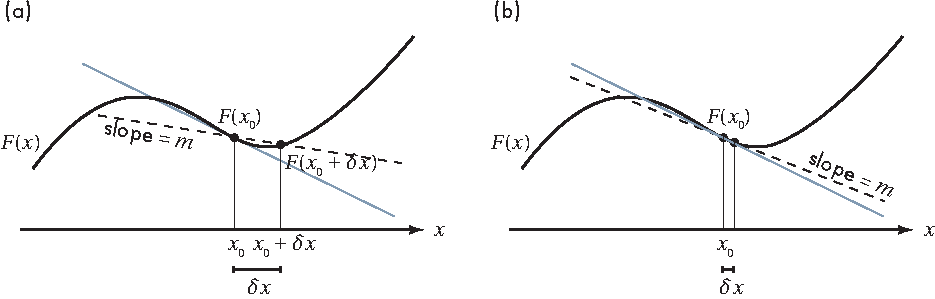
\includegraphics[]{math_primer/figures/dx.pdf}
  }
  \caption{Derivatives of functions.  The {\it slope} of a function at a point,
  $x_{0}$, can be approximated by taking the difference of the function
  evaluated at the point, $F(x_{0})$, and a nearby point, $F(x_0 + \delta\! x)$,
  divided by the distance, $\delta\! x$ between them.  The {\it derivative}
  represents the slope in the limit where $\delta\! x$ goes to 0.}
  \label{fig:dx}
\end{figure}

\subsubsection{Example}
Let us choose a simple function $F(x) = x^2$ as an example.  If we evaluate the
slope between $x_{0}$ and $x_{0} + \delta\! x$ we obtain
\begin{align*}
    m & \approx \frac{(x_0 + \delta\! x)^{2} - x_0^2}{\delta\! x} \\
      & \approx \frac{x_0^{2} + 2 x_0 \delta\! x + \delta\! x^{2} - x_0^2}{\delta\! x} \\
      & \approx \frac{2 x_0 \delta\! x + \delta\! x^2}{\delta\! x} \\
      & \approx 2 x_0 + \delta\! x.
\end{align*}
Applying the definition of the derivative (Equation~\ref{eq:derivative}),
\begin{equation*}
    \lim_{\delta\! x \to 0} (2 x_0 + \delta\! x) = 2 x_0.
\end{equation*}
Hence the slope (derivative), $m$, at the point of interest, $x_{0}$, is
\begin{equation*}
    m = \left. \dv{x^2}{x} \right|_{x = x_0} = 2 x_0.
\end{equation*}
For this function we can write the derivative at any point as
\begin{equation*}
    \dv{x^2}{x} = 2 x.
\end{equation*}

Derivatives can be a bit more difficult when the functions are not continuous or
smooth (a.k.a.\ not differentiable).  However, we often do wish to know the
derivative at these points in geophysics because they represent the boundaries
and interfaces---or discrete changes in behaviour with time---between
formations/rock types and their properties or their response to a physical
process.  In these cases, we often play games like taking the derivative from
each side of the boundary separately.  You have already seen this done as it was
performed on our circuit analogy with $\dd{u}\dd{t}$.  The function for the
changing transmitter current, $u(t)$, is continuous but not smooth.  For each
smooth segment of $u(t)$ the derivative is treated independent of the others
which resulted in three distinct behaviors within the conductive body.

\subsection{Chain Rule} \label{calc:chain}
There are few properties of derivatives more useful than the chain rule.  The
chain rule allows us to rewrite a complex function as a composite of simpler
functions.  Suppose we have a function $F(x)$ that we can write as a composite
of two or more functions, that is suppose we have another function $G(x)$ such
that $F(x) = F[G(x)]$.  Some examples of composite functions include,
\begin{align*}
    G(x) &= \sin x & F[G(x)] &= e^{G(x)} \\
    && &= e^{\sin x} ,
\end{align*}
\begin{align*}
    H(x) &= x^2 + z^2 & G[H(x)] &= H(x)^{1/2} & F\{G[H(x)]\} &= \frac{1}{G[H(x)]} \\
    && && &= \frac{1}{H(x)^{1/2}} \\
    && && &= \frac{1}{(x^2 + z^2)^{1/2}} .
\end{align*}

To find the derivative of such a function, we apply the chain rule,
\begin{equation*}
    \dv{}{x}F[G(x)] = \dv{F}{G}\dv{G}{x},
\end{equation*}
or more generally for a multiply compound function,
$f_0(f_1(f_2(\ldots f_{n-1}(f_n(x))\ldots))$,
\begin{equation}
    \dv{}{f_0(x)} = \dv{}{x}[f_0(f_1(f_2(\ldots f_{n-1}(f_n(x))\ldots))] =
    \dv{f_0}{f_1}\dv{f_1}{f_2}\cdots\dv{f_{n-1}}{f_n}\dv{f_n}{x} .
\end{equation}
What this allows us to do is take a complex function and break it into simpler
elements that can be easily differentiated (or at least make the derivatives
look like the forms given in a table of derivatives like the one located at the
end of this tutorial).

\subsubsection{Example}
Let's apply the chain rule to the second function above.  In order to find
$\dv{F}{x}$, we need the derivatives of $\dv{F}{G}$, $\dv{G}{H}$, and
$\dv{H}{x}$, all of which are general forms that we can find the table of
derivatives,
\begin{align*}
    1: && \dv{F}{G} &= \dv{}{G} \frac{1}{G} \\
    && &= -\frac{1}{G^2} \\
    2: && \dv{G}{H} &= \dv{}{H} H^{1/2} \\
    && &= \frac{1}{2 H^{1/2}} \\
    3: && \dv{H}{x} &= \dv{}{x} (x^2 + z^2) \\
    && &= 2 x.
\end{align*}
Now, we multiply each together and substitude each composite function to obtain
the derivative,
\begin{align*}
    \dv{F}{x} &= \dv{F}{G} \dv{G}{H} \dv{H}{x} \\
    &= \left(-\frac{1}{G^2}\right) \left(\frac{1}{2 H^{1/2}}\right) (2 x) \\
    &= \left(-\frac{1}{H^{\frac{1}{2} \cdot 2}}\right)
    \left(\frac{1}{2 (x^2 + z^2)^{1/2}}\right) 2 x \\
    &= \left(-\frac{1}{(x^2 + z^2)}\right)
    \left(\frac{1}{2 (x^2 + z^2)^{1/2}}\right) 2x,
\end{align*}
and finally simplifying,
\begin{equation*}
    \dv{F}{x} = - \frac{x}{(x^2 + z^2)^{3/2}} .
\end{equation*}

\subsection{Higher-order and partial derivatives}
There are also times when we wish to take higher order derivatives (e.g.\
acceleration is the second derivative of a distance function dependent upon
time).  In these cases the derivative operation is performed multiple times and
is mathematically represented by
\begin{equation}
    \dv[n]{}{x} F(x).
\end{equation}

A function may be dependent on multiple independent variables.  For example,
$F(x,y) = x^3y + y^2$ is a function of both $x$ and $y$.  We may take the
derivative of one or the other variables while treating the second constant.  We
call this operation the partial derivative where we use the symbol $\partial$ in
place of $d$.  For the above equation, the partial derivatives are
\begin{align*}
    \pdv{}{x}F(x,y) & = 3x^2y \\
    \pdv{}{y}F(x,y) & = x^3 + 2y.
\end{align*}
We can also take multiple derivatives in only one variable or both,
\begin{align*}
    \pdv[2]{}{x} F(x,y) & = 6xy \\
    \pdv[2]{}{y} F(x,y) & = 2 \\
    \frac{\partial^2}{\partial x \partial y} F(x,y) = 
    \frac{\partial^2}{\partial y \partial x} F(x,y) & = 3x^2. \\
\end{align*}
Note that when taking mixed derivatives, the result is independent of the order
in which the partials are taken.

\subsection{Table of Common Derivatives}
\begin{framed}
\noindent Derivatives of a few common functions (note $u = u(x)$, $v = v(x)$,
$a$ and $n$ are constants):
\begin{flalign*}
    &\dv{}{x}(a) = 0 &
    &\dv{}{x}(x) = 1 \\
    &\dv{}{x}(au) = a \dv{u}{x} &
    &\dv{}{x}(u + v) = \dv{u}{x} + \dv{v}{x} \\
    &\dv{}{x}(uv) = v\dv{u}{x} + u\dv{v}{x} &
    &\dv{}{x}\left(\frac{u}{v}\right) = v^{-2}\left(v\dv{u}{x} - u\dv{v}{x}\right) \\
    &\dv{}{x}u(v) = \dv{u}{v}\dv{v}{x} &
    &\dv{y}{x} = \left( \dv{x}{y} \right)^{-1} \\
    &\dv{}{x}(u^n) = n u^{n-1} \dv{u}{x} &
    &\dv{}{x}\left(\frac{1}{u^n}\right) = -\frac{n}{u^{n + 1}} \dv{u}{x} \\
    &\dv{}{x}(e^u) = e^u \dv{u}{x} & 
    &\dv{}{x}(\log u) = \frac{1}{u} \dv{u}{x},\; u > 0 \\
    &\dv{}{x}(\sin u) = \cos u \dv{u}{x} &
    &\dv{}{x}(\cos u) = -\sin u \dv{u}{x}
\end{flalign*}
\end{framed}



% ---------------------------------------
\section{Integrals} \label{apx:integral}
\subsection{Definition}
Integrals (anti-derivatives) perform the inverse operation of a derivative.  Its
technical definition is
\begin{equation*}
    \dv{}{x} \int_{0}^{x} f(t) \dd{t} \equiv f(x),
\end{equation*}
and while this is accurate and establishes that integration is in fact the
anti-derivative, it is basically useless for understanding how it works.  So
lets approach the integral from another way.

If a derivative represents the differences of small steps, integrals represent
the sum of small steps.  Since we divided before by $\delta x$, this time we
will do the opposite and multiply, suggesting that the integral represents an
area under a curve (Figure~\ref{fig:ix}).
\begin{figure}[hbt]
  \centerline{
    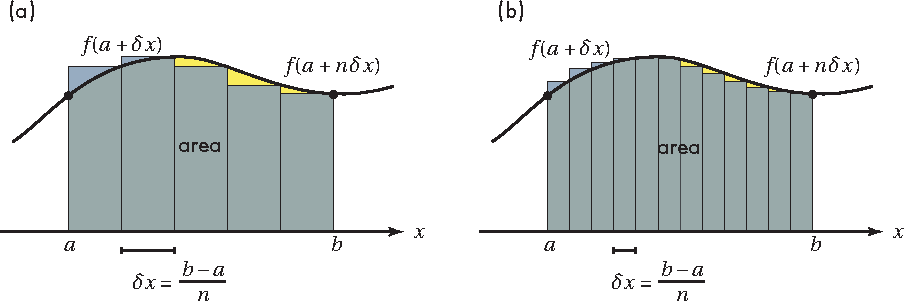
\includegraphics[]{math_primer/figures/ix.pdf}
  }
  \caption{Integrals of functions.  The {\it area} under a function between two
  points, $a$ and $b$, can be approximated by the sum of $n$ small columns with
  height $f(a + i \delta\!  x)$ and width $\delta\! x = (b - a)/n$.  The {\it
  integral} represents the area in the limit where $n$ goes to infinity.}
  \label{fig:ix}
\end{figure}

Consider a function $f(x)$ finite on the interval $[a, b]$ ($a \leq x \leq b$).
A simple method for approximating the area is performed by dividing the curve
into several rectangular elements and summing the individual area of each.  For
$n$ steps in $x$, the width of the step is $\delta\! x = (b - a)/n$.  To find
the area of each element, we multiply the step size, $\delta\! x$ by the value
of the function within the $i$-th step, $f(\bar{x}_i)$.  It does not matter
where we choose the value of the function so long as it is between the interval
bounds, $x_i$ to $x_{i+1}$, because as the interval width appoaches zero the
value of the fuction on each side of the interval approach the same value.
Summing each element gives an estimate of the total area, 
\begin{equation*}
    A \approx \sum_{i = 1}^{n} f(\bar{x}_{i}) \delta x.
\end{equation*}
A more useful definition for the purposes of determining an integral employs the
limit as $n$ goes to infinity ($\infty$),
\begin{equation*}
    \int_{a}^{b} f(x) \dd{x} \equiv \lim_{n \to \infty} \sum_{i = 1}^{n}
        f(\bar{x_{i}}) \frac{b - a}{n}.
\end{equation*}

There are a few integrals that are quite common and tend to show up frequently
in derivations.  The solutions to these integrals are commonly listed in `{Tables
of Integrals}' which you can easily find using a web search under the same name.
You will find thousands all of which are 95\% the same.  Mathworld has a pretty
good one, as does Wikipedia.  I use a copy of the Standard Mathematical Tables
and Formula from the CRC Press.

\subsection{Example}
Consider the result from our derivative example, $f(x) = 2 x$, we will integrate
this result to (1) illustrate how an integral is determined by a sum of
infinitely man small areas
and (2) show that the integral of a derivative has the same form of our original
function.

As we discussed above, the area of a column is given by the height,
found by evaluating our function some point within the bounds of th column,
multiplied by the width of the column, i.e.,
\begin{align*}
    A_i &\approx f(\bar{x}_i) \delta\! x \\
    &\approx 2 \bar{x}_i \delta\! x .
\end{align*}
The total area of all the columns is then
\begin{align*}
    A &\approx A_1 + A_2 + A_3 \ldots A_n \\
    &\approx \sum_{i=1}^n A_i .
\end{align*}
Therefore, including the individual areas in terms of our function as above, the
sum becomes
\begin{equation*}
    A \approx \sum_{i = 1}^{n} 2 \bar{x}_i \delta\! x .
\end{equation*}
If we choose $\bar{x}_i$ at a convenient location, say at the lower bound to the
column width.  The $x$ coordintes that the function is evaluated at are $a$, $a
+ \delta\! x$, $a + 2\delta\! x$ and so on.  This allows us to write the area
as,
\begin{align*}
      A &\approx \left[ 2 (a + \delta\! x) + 2 (a + 2 \delta\! x) 
        + \ldots + 2 (a + n \delta\! x) \right] \delta\! x \\
      &\approx \sum_{i = 1}^{n} (2 a \delta\! x + 2 i \delta\! x^2).
\end{align*}
The first sum is trivial, the second requires knowing that $\sum_{i=1}^{n} i = n
(n + 1)/2$.  Thus the summation becomes
\begin{equation*}
    A \approx 2 a n \delta\! x + n (n + 1) \delta\! x^2.
\end{equation*}
Now inputting the definition of $\delta\! x$, we have
\begin{align*}
    A & \approx 2 a n \frac{b - a}{n} + n (n + 1) \frac{(b - a)^2}{n^2} \\
      & \approx 2 a (b - a) + \left( 1 + \frac{1}{n} \right) (b - a)^2 \\
      & \approx 2 a b - 2 a^2 + (b - a)^2 + \frac{(b - a)^2}{n} \\
      & \approx 2 a b - 2 a^2 + b^2 - 2 a b + a^2 + \frac{(b - a)^2}{n} \\
      & \approx b^2 - a^2 + \frac{1}{n}(b - a)^2 \\
\end{align*}
Now we can introduce the limit again only it as the number of intervals goes to
infinity,
\begin{equation*}
    \lim_{n \to \infty} b^2 - a^2 + \frac{1}{n}(b - a)^2 = b^2 - a^2.
\end{equation*}
Therefore, the integral from $a$ to $b$ of $2 x$ is
\begin{equation*}
    \int_{a}^{b} 2 x \dd{x} = \left. x^2 \right|_{a}^{b} = b^2 - a^2.
\end{equation*}

We have now shown that the integral in this case is indeed the anti-derivative.
Another important implication is that the integral depends only upon the bounds
of integration, $a$ and $b$, which is true in general and not just for this
example.

\subsection{Indefinite integrals}
The above result is called the definite integral because it has defined limits
of integration, but there are many times we wish to have arbitrary integration
limits.  When the limits are arbitrary we call this the indefinite integral, and
it is written as
\begin{equation}
    \int f(x) = F(x) + C.
\end{equation}
For our previously worked example, the indefinite integral is
\begin{equation*}
    \int 2 x \dd{x} = x^2 + C,
\end{equation*}
where $C$ is an arbitrary constant.  The constant arises from the fact that a
derivative of a constant is 0, so the general anti-derivative must allow for
the possibility of a constant that vanished under the derivative operation.

\subsubsection{Example}
Let us take the function,
\begin{equation*}
    f(x) = x e^{-x^2} .
\end{equation*}
To take the integral,
\begin{equation*}
    \int f(x) \dd{x} = \int x e^{-x^2} \dd{x} ,
\end{equation*}
we need to put the integral into a form that we can find in an integral table.
Looking at the table of integrals, the closest integral we can find is
\begin{equation*}
    \int e^u \dd{u} = e^u \dd{u} .
\end{equation*}
We will also need the integral property,
\begin{equation}
    \int u(v) \dd{x} = \int u \left(\dv{v}{x}\right)^{-1} \dd{v} ,
\end{equation}
to rewrite our function into the simplified form we desire.  So let us define a
function
\begin{align*}
    v(x) &= -x^2 \\
    \dv{v}{x} &= -2x \\
    - \frac{1}{2x} \dd{v} &= \dd{x} .
\end{align*}
Substituting in the $v(x)$ and the expression for $\dd{x}$, we find 
\begin{equation*}
    \int x e^{-x^2} \dd{x} = \int x e^{v} \left( - \frac{1}{2x} \dd{v} \right) .
\end{equation*}
Simplifying and bringing the constants outside the integral,
\begin{equation*}
    \int x e^{-x^2} \dd{x} = - \frac{1}{2} \int e^{v} \dd{v} \\
\end{equation*}
Since this now looks like our elementary form, all we need to do is complete the
integration and back subsitute the $v(x)$.
\begin{align*}
    \int x e^{-x^2} \dd{x} &= - \frac{1}{2} e^{v} \\
    &= - \frac{1}{2} e^{-x^2} .
\end{align*}


\subsection{Multiple integrals}
Again there are times where we wish to integrate multiply say for area
(2-dimensional) or volume (3-dimensional) calculations.  The area can be written
\begin{equation}
    \iint f(x,y) \dd{x} \dd{y} = \int_{A} f(x,y) \cdot \dd{\vb{a}},
\end{equation}
where $\dd{\vb{a}}$ implies area infintesimals and for volume,
\begin{equation}
    \iiint f(x,y,z) \dd{x} \dd{y} \dd{z} = \int_{V} f(x,y,z) \cdot \dd{\vb{v}},
\end{equation}
where $\dd{\vb{v}}$ implies volume infintesimals.  Note that the order in which
we perform the integrations is irrelevant to the solution (although in reality,
our choice of order may make it easier to derive).

\begin{framed}
    {\bf Aside:} In reality, the derivative or integral of a function may be
    very complex, or we do not know {\it a priori} (beforehand) the exact nature
    of the originating function.  In these cases, we use numerical techniques
    not terribly dissimilar from the original algebraic starting points, i.e.\
    with differences and sums of small intervals.
\end{framed}

A table of integrals is often far handier than a table of derivatives since the
chain rule can be successively applied to make each step closer to an elementary
form.  To give you an indication how much more challenging integrals can be, the
table of derivatives in the {\it Standard Mathematical Tables and Formulae}
covers common derivatives in two pages and provides 44 pages of integrals.  But
never fear, we will only use a few and if use one not in the table, I will
provide you with the relevant general forms if you need them to complete
problems.

\subsection{Table of Common Integrals}
\begin{framed}
\noindent Integrals of a few common functions (note $u = u(x)$, $v = v(x)$,
$a$ and $n$ are constants and $C$ is an arbitrary constant due to integration):
\begin{flalign*}
    &\int a \dd{x} = a x + C &
    &\int x \dd{x} = \frac{1}{2}x^2 + C \\
    &\int au \dd{x} = a \int u \dd{x} &
    &\int (u + v) \dd{x}  = \int u \dd{x} + \int v \dd{x} \\
    &\int u \dd{v} = uv - \int v \dd{u} &
    &\int u(v) \dd{x} = \int u(v) \left( \dv{v}{x} \right)^{-1} \dd{v} \\
    &\int u^n \dd{u} = \frac{1}{n+1} u^{n+1} + C, \; n \neq -1 &
    &\int \frac{1}{u} \dd{u} = \log u + C \\
    &\int e^{u} \dd{u} = e^{u} + C &
    &\int \log u \dd{u} = u \log u - u \\
    &\int \sin u \dd{u} = -\cos u + C &
    &\int \cos u \dd{u} = \sin u + C 
\end{flalign*}
\end{framed}


\nocite{Zwillinger1996}
\bibliographystyle{elsarticle-harv}
\bibliography{ref}

\chapter{Vector Calculus: What is the fastest way downhill?} \label{apx:vcalc}

\section{The $\grad$ (del) operator}

The differential operator, del ($\nabla$), is a convenient way to represent
multiple partial derivatives in a compact form.  Several operations are common
using $\nabla$: the gradient ($\mbox{grad}$) of a scalar function, $f$, is given
by
\begin{equation}
    \mbox{grad}\; f(x,y,z) = \grad f = \pdv{f}{x}\vu{x} + \pdv{f}{y}\vu{y} +
        \pdv{f}{z}\vu{z},
\end{equation}
which yields a vector with direction of the indicated by the unit vectors
$(\vu{x}, \vu{y}, \vu{z})$; the divergence ($\mbox{div}$) of a vector
function, $\vb{A}$, is given by
\begin{equation}
    \mbox{div}\; \vb{A}(x,y,z) = \div \vb{A} =
        \pdv{A_x}{x} + \pdv{A_y}{y} + \pdv{A_z}{z},
\end{equation}
which yields a scalar; and the curl of a vector function is given by
\begin{equation}
    \mbox{curl}\; \vb{A}(x,y,z) = \curl \vb{A} = 
        \left( \pdv{A_z}{y} - \pdv{A_y}{z} \right) \vu{x} +
        \left( \pdv{A_x}{z} - \pdv{A_z}{x} \right) \vu{y} +
        \left( \pdv{A_y}{x} - \pdv{A_x}{y} \right) \vu{z},
\end{equation}
which yields a vector.  Because the definition of the curl can be difficult to
remember, it can also be represented as the determinant,
\begin{equation*}
    \curl \vb{A} =
    \begin{vmatrix}
        \vu{x} & \vu{y} & \vu{z} \\
        \pdv{}{x} & \pdv{}{y} & \pdv{}{z} \\
        A_{x} & A_{y} & A_{z}
    \end{vmatrix}
    = \left( \pdv{A_z}{y} - \pdv{A_y}{z} \right) \vu{x} +
    \left( \pdv{A_x}{z} - \pdv{A_z}{x} \right) \vu{y} +
    \left( \pdv{A_y}{x} - \pdv{A_x}{y} \right) \vu{z},
\end{equation*}

A graphical description of the divergence and curl of a
vector field in relation to a point are illustrated in Figure~\ref{fig:divcurl}.
\begin{figure}[hbt]
  \centering
  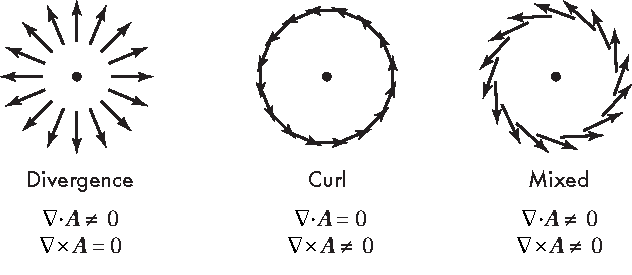
\includegraphics[]{math_primer/figures/div_grad_curl.pdf}

  \caption{The divergence and curl of a vector field.  The terms convergence
  (now divergence) and curl were actually suggested by Maxwell for vector
  operations.  The vector field on the left exhibits pure divergence; all the
  vectors point normal to the point.  The vector field in the center illustrates
  pure curl; all the vectors are parallel the point inducing a circulation about
  the point.  The vector field on the right is mixed with both non-zero
  divergence and curl.}
  \label{fig:divcurl}
\end{figure}

Another important relation is the Laplacian operator and is particularly useful
in potential fields,
\begin{equation}
    \div \grad f = \nabla^{2} f = \pdv[2]{f}{x} + \pdv[2]{f}{y} + \pdv[2]{f}{z}.
\end{equation}
For a thorough (but quite readable) treatment of the $\nabla$ operator, I refer
you to \citet{Schey1997}.

These terms (other than Laplacian) were devised because they attempt to convey a
physical meaning to the mathematics.  Consider the topography of a mountain.
Every point on the mountain can be thought of in terms of the elevation of that
point.  The collection of the elevation points is a scalar function or scalar
`field' that we of course call the topography.  The gradient of the topography
is simply the slope at a given point.

Taking our topography example, lets place a marble at every point on the
surface.  The marbles are instantaneously moving down the direction of the
maximum slope.  At a local high point, a peak, all the marbles nearest the peak
are moving away from each other or diverging.  At a local low, a valley, all the
marbles are moving towards each other (converging).  The divergence tells us how
much the velocity fields concentrate or disseminate the marbles.

It is a bit more difficult to come up with an example of the curl using our
topography example.  Instead think of a pinwheel in the wind.  As the wind
blows, the point on the pinwheel tries to move in the direction of the wind is
blowing but cannot because it is attached to the surface.  The force of the wind
against this point then imparts a torque about the point causing a net rotation
(or curl).

There are some vector identities that can be derived from various combinations of
the $\nabla$ operator.  One that we use in EM geophysics is
\begin{equation}
    \curl \curl \vb{A} = \grad(\div \vb{A}) - \nabla^{2} \vb{A}.
    \label{eq-curlcurl}
\end{equation}

\section{Contour Integrals} \label{apx:cintegral}
The integral form of Maxwell's equations uses notation $\fint{C}{}$\ or
$\fint{S}{}$, in several places which denote a line integral and surface
integral, respectively.  When the line (contour) or surface are enclosed
$\cint{}$\ is used, and is only valid when the entire path or surface are
included in the integration.

\bibliographystyle{elsarticle-harv}
\bibliography{ref}


%\singlespace
%\bibliographystyle{elsarticle-harv}
%\bibliography{ref}
%\endsinglespace

\end{document}
